% --------------------------------------------------------------------
%
% This is a book. It isn't style with the swiss army knife equivalent of a document
% class (memoir), because it was clashing with the glossaries package
%
% --------------------------------------------------------------------

\documentclass[11pt, b5paper, twoside, openright, onecolumn]{book}

% we will generate slightly different PDF files based on whether this is a draft or not
\usepackage{ifthen}
\newcommand{\true}{true}
\newcommand{\false}{false}
\newcommand{\draft}{\true}
\newcommand{\ifdraft}[1]{\ifthenelse{\equal{\draft}{\true}}{#1}{}}
\newcommand{\notdraft}[1]{\ifthenelse{\equal{\draft}{\false}}{#1}{}}

%	set up page dimensions. normally, inner margin < outer margin.
%	This makes no sense, since the binding is on inner. As such, reverse these two.
%
%	For draft copies, [inner:outer] ratio is kept [1:1], for publication this is set to [2:1]
%	to compensate for the lost space due to binding
%

\ifdraft{\usepackage[b5paper, bindingoffset=0mm, inner=17mm, outer=17mm, top=21mm, bottom=24mm,driver=xetex]{geometry}}
\notdraft{\usepackage[b5paper, bindingoffset=0mm, inner=23mm, outer=11mm, top=21mm, bottom=24mm,driver=xetex]{geometry}}

%	half inch paragraph indentation

\setlength{\parindent}{0.5in}

%	using "draft" mode as document class option seriously interferes with images,
%	so instead we just do a switch so we get a visual clue when overfull hboxes occur

\ifdraft{\overfullrule=5pt}

%	for publication, because my POD printer requires it, the content is centered on letter size pages

\notdraft{
	\usepackage[letter,center]{crop}
	%	some quick hackery: intercharclasses should NOT interfere with the "crop" package,
	%	so whenever we use a picture, we turn off intercharclass behaviour
	\let\latexpicture=\picture
	\def\picture{\XeTeXinterchartokenstate=0 \latexpicture}
}


\usepackage{tocloft}			% what book doesn't have a ToC?

\usepackage{appendix}			% clearly we need appendices
\noappendicestocpagenum		% no page number for the general ToC heading "Appendices"

\usepackage{longtable}			% used for tables that run past a page
\usepackage{needspace}		% required to make sure longtable doesn't generate
						% an orphaned footer/header pair across two pages.

\usepackage{fontspec}			% using system fonts is far better than using plain tex fonting~!
\usepackage{relsize}			% this really should already be part of standard LaTeX, rather than requiring a package
\renewcommand\RSsmallest{5pt}	% relzise goes to 6pt as minimum by default, but that won't cover \tiny, so we set it 5

\usepackage{color}			% colors are used for debugging purposes
\usepackage{float}			% figures
\usepackage{graphicx}			% figures

\setlength\fboxsep{5pt}
\setlength\fboxrule{0.3mm}		% mainly the border around images

% ----------------------------------------------------------------
% which fonts to use, and when
% ----------------------------------------------------------------

\input{includes/xelatex/interchar.preamble}
\setmainfont{Palatino Linotype}

% ----------------------------------------------------------------
% ruby markup stuff
% ----------------------------------------------------------------

\usepackage{accsupp}
\usepackage[xetex, pdfborder=0 0 0]{hyperref}% has to be loaded as late as possible...

% ----------------------------------------------------------------
% ruby and rubystack for for use in tables.
% This needs extra spacing to ensure visually appealing alignment,
% but rather than using an extra argument, it figured it'd be more
% readable, and overall less space-taking to just copy the plain
% macro and rename it
% ----------------------------------------------------------------

\newcommand*{\rtrubystack}[2]{{\relscale{0.5}%
  \begin{tabular}[b]{@{}c@{}}%
    {#1}\\%
    {\textscale{2}{#2}}%
  \end{tabular}}%
}

\DeclareRobustCommand*{\rtruby}[2]{%
  \mbox{%
    \setlength{\parskip}{0ex}%
    \BeginAccSupp{method=pdfstringdef,ActualText={#1}}%
      \rtrubystack{\phantom{#2}}{#1}%
      \llap{%
        \rtrubystack{#2}{\phantom{#1}}%
      }%
    \EndAccSupp{}%
  }%
}

% --------------------------------------------------------------
% ruby and rubystack macro, effecting ghost furigana in the PDF
% --------------------------------------------------------------

\newcommand*{\rubystack}[2]{{\relscale{0.5}%
  \begin{tabular}[b]{@{}c@{}}%
    {#1}\\%
   {\textscale{2}{#2}}%
  \end{tabular}}%
}

\DeclareRobustCommand*{\ruby}[2]{%
  \mbox{%
    \setlength{\parskip}{0ex}%
    \BeginAccSupp{method=pdfstringdef,ActualText={#1}}%
      \rubystack{\phantom{#2}}{#1}%
      \llap{%
        \rubystack{#2}{\phantom{#1}}%
      }%
    \EndAccSupp{}%
  }%
}

% --------------------------------------------------------------------------
% helper macro: adds space between the text and the [T]op \hline in a table
% --------------------------------------------------------------------------

\newcommand\T{\rule{0pt}{2.5ex}}% zero width, 2.5ex vertical spacing, ensures a visually appealing vertical alignment

% ------------------------
% disable commands for PDF
% ------------------------

\pdfstringdefDisableCommands{%
  \renewcommand*{\rtruby}[2]{#2 (#1)}% #1 for base, #2 for just furi, #2 (#1) for the logical choice =)
  \renewcommand*{\ruby}[2]{#2 (#1)}%
}

% ----------------------------------------------------------------
% set up lists to, by default, have no bullet symbol... as it should be!
% ----------------------------------------------------------------

\renewcommand{\labelitemi}{}

% ----------------------------------------------------------------
% example blocks may not be broken up. so they're in a minipage,
% and their lines will end in \\*
% ----------------------------------------------------------------

\newenvironment{exampleblock}{
\setlength{\parindent}{0.6in}
\begin{minipage}[t]{\dimexpr\textwidth-\parindent}}
{\end{minipage}}

% ----------------------------------------------------------------
% always indented table
% (indented regardless of paragraphing in sections)
% ----------------------------------------------------------------

\newenvironment{mytabular}[1]{\noindent\hspace{0.4in}
\begin{tabular}[h]{#1}}{\end{tabular}}

% ----------------------------------------------------------------
% always centered table
% (not indented, regardless of paragraphing in sections)
% ----------------------------------------------------------------

\newenvironment{mytabularcentered}[1]{\noindent
\begin{center}\begin{tabular}[h]{#1}}{\end{tabular}\end{center}}

% ----------------------------------------------------------------
% vertical writing (disable intercharclasses here)
% ----------------------------------------------------------------

\usepackage{includes/xelatex/vertical}

% ----------------------------------------------------------------
% set up glossary
% ----------------------------------------------------------------

% use glossary

\usepackage{glossaries}% glossaries has to be loaded after hyperref, or things go wrong
\renewcommand*{\glossaryentrynumbers}[1]{}
\makeglossaries

% glossary terms placeholder (filled by texate.php script)
\newglossaryentry{glossary}{ name={Glossary}, description={}}
\newglossaryentry{abstraction}{ name={Abstraction}, description={A generalisation‚ either through simplification(s) or by omission(s) of some (or more) part(s). For instance‚ the concept of “friendship” is an abstraction from all the individual instances of people being friends (an abstraction by generalisation). Similarly‚ the concept of “walking” is an abstraction of the concerted effort of all the muscles moving in the human body to effect that body walking on two legs (an abstraction by omission‚ because for “walking”‚ all the unrelated information of muscles working‚ the brain balancing the body‚ the eyes determining the direction of travel‚ etc. is irrelevant)‚ and the Japanese kana are abstractions of Chinese characters (either by simplification in the case of hiragana‚ or omission in the case of katakana).}}
\newglossaryentry{accent}{ name={Accent}, description={Accent in speech is that part of a word that seems to jump out at the listener‚ placing more focus on one or more syllables than on the rest of the word. For instance‚ the word “attention” has its accent on “ten” in English‚ while the accent lies on “on” in French. Accents are typically in the form of a noticeably different pitch level or gradient for the syllable(s) in question than for the rest of the word.}}
\newglossaryentry{accusative}{ name={Accusative}, description={In this book‚ ‘accusative’ is used in the natural language meaning‚ not the grammatical meaning‚ representing a construction that accuses someone of something. The grammatical “accusative” form refers to the role of a direct object to a word that can take such direct objects (which typically means verbs).}}
\newglossaryentry{active}{ name={Active}, description={The verb form that describes actions taking place in the world‚ as performed by someone or something. For instance “I throw the ball” describes an activity performed by me. Contrast to “passive”.}}
\newglossaryentry{adverb}{ name={Adverb}, description={Words that are used to describe the way in which a verb action or state is in effect. For instance‚ “To walk quickly” has the adverb “quickly” describing the way in which “walking” is performed.}}
\newglossaryentry{affirmative}{ name={Affirmative}, description={A word or part of phrase that states (“asserts”) something is the case. Contrast to “negative”.}}
\newglossaryentry{animate}{ name={Animate}, description={The quality of things that allows us to say they are alive‚ or seem lifelike. This covers not just things like people or animals‚ but also things that seem to move on their own‚ or even things which possess a “lively” quality‚ such as an animate conversation. Contrast to “inanimate”.}}
\newglossaryentry{article}{ name={Article}, description={A particular kind of word that references particular objects. In English‚ these are the indefinite articles “a” and “an” and the definite article “the”.}}
\newglossaryentry{assertive}{ name={Assertive}, description={Bold‚ confident‚ or even aggressively self-assured.}}
\newglossaryentry{attributive}{ name={Attributive}, description={Attributing a particular quality to something. For instance‚ used attributively‚ the word “blue” in the phrase “The blue book” attributes the quality “blue” to the object “book”. Common attributive word classes include the adjectives (attributing quality to nouns) and adverbs (attributing qualities to verbs).}}
\newglossaryentry{auxiliary verb}{ name={Auxiliary verb}, description={A verb that is used to give additional meaning to another verb. For instance‚ in the English phrase “I can do this”‚ the verb “can” is an auxiliary verb‚ combining with “do” to form a potential form‚ rather than a plain predicative form. These may also be referred to as ‘helper verbs’.}}
\newglossaryentry{binary}{ name={Binary}, description={Anything in which only two choices can be made‚ such as binary signals (high and low)‚ binary numbers (zero or one) or any arbitrary choice (“one or the other”). Notice that no choice is ever truly binary‚ since there is always the choice to not pick either‚ and sometimes even allowing both to be picked‚ thus making binary choices secretly ternary choices‚ and  sometimes even quaternary choices.}}
\newglossaryentry{cardinal}{ name={Cardinal}, description={A cardinal number differs from a normal number in that it refers to a number belonging to a particular set. Contrast this to ordinal numbers‚ which indicate a number is part of some sequence. For example‚ if we have a collection of 10 marbles marked 1 through 10‚ then the marble with number 6 written on it has cardinal number 6. However‚ if we look at in which order we can take the marbles out of some container and the marble marked with the number 6 is the first marble we pull out‚ then its ordinal number is 1 (because it’s the first in the series of “drawn marbles”)‚ but its cardinal number is still 6 (because it’s still marble 6 in the collection of marbles).}}
\newglossaryentry{clause}{ name={Clause}, description={A group of words that contain a subject and a predicate‚ but do not form a full sentence.}}
\newglossaryentry{cohortative}{ name={Cohortative}, description={A word form or construction that suggests performing some action. In English‚ cohortatives are typically statements such as “shall we ...?” or “let’s ...”.}}
\newglossaryentry{colloquial}{ name={Colloquial}, description={Spoken conversation‚ usually used to mean the informal spoken version of a language‚ as contrasted to formal language.}}
\newglossaryentry{commanding}{ name={Commanding}, description={A word form or construction that commands the listener or reader to perform some action. Contrast to “prohibiting”.}}
\newglossaryentry{comparative}{ name={Comparative}, description={A word form or form of phrase that compares one or more things to each other in some way.}}
\newglossaryentry{compound}{ name={Compound}, description={A word that has been formed by combining two or more words.}}
\newglossaryentry{conditional}{ name={Conditional}, description={A word form or construction that indicates something is dependent on something else happening‚ or being a particular way. The general description is in the form “If A‚ then B”‚ with A representing a condition‚ and B representing the consequence should the condition be met.}}
\newglossaryentry{conjugation}{ name={Conjugation}, description={A derived form of a verb‚ adjective or noun through inflection‚ either by modification‚ additions‚ or both.}}
\newglossaryentry{conjugational bases}{ name={Conjugational bases}, description={A conjugational base is the most basic verbal “building block” in Japanese grammar‚ upon which all verbal inflections are built. These are: 1) the 未然形(みぜんけい)‚ imperfect base‚ 2) the 連用形(れんよけい)‚ continuative base‚ 3) the 終止形(しゅうしけい)‚ finalising base‚ 4) the 連体形(れんたいけい)‚ attributive base‚ 5) the 已然形(いぜんけい)‚ perfective base‚ and 6) the 命令形(めいれいけい)‚ commanding base. \\ Of these‚ the 終止形 is no longer used‚ and the 已然形 is also referred to as the 仮定形(かていけい) (potential base) in modern Japanese‚ as it is only used for hypothetical constructions.}}
\newglossaryentry{connotation}{ name={Connotation}, description={The commonly understood meaning of a word or phrase‚ rather than its literal meaning. For instance‚ “take a chair” connotes sitting down‚ rather than the literal taking of a chair. Contrast to “denotation”.}}
\newglossaryentry{context}{ name={Context}, description={All information‚ both explicit and implied‚ that indicates how to interpret pronouns and referential information in one or more sentences.}}
\newglossaryentry{continuative}{ name={Continuative}, description={An inflection indicating that the action represented by the inflected word is still in effect‚ either ‘as is’‚ or as part of a more complex inflection.}}
\newglossaryentry{contraction}{ name={Contraction}, description={The phenomenon in which certain parts of speech get shortened by either dropping (series of) syllables or replacing series of syllables with shorter‚ different syllables. An example of this in English is the word “cannot” being turned into “can’t” through omission. An example in Japanese is なければ being turned into なきゃ through a combination of omission and replacement.}}
\newglossaryentry{contrasting}{ name={Contrasting}, description={Showing two things as being different in one or more respects. The biggest possible contrast is called polar contrast‚ where two things are presented as opposites (‘lying on opposite poles’)‚ rather than merely differing.}}
\newglossaryentry{copula}{ name={Copula}, description={A word or part of phrase used to define‚ or couple‚ things. In English‚ this is the verb “to be”‚ which is used in definitions‚ such as “the sky is blue”. In Japanese‚ these are a large number of copulae‚ with the two words だ and です being the most used‚ for informal and formal coupling respectively.}}
\newglossaryentry{counter}{ name={Counter}, description={A word used to indicate that a numerical statement should be considered as representing a count of some thing(s)‚ rather than a plain number.}}
\newglossaryentry{decomposition}{ name={Decomposition}, description={Reducing compound constructions to their individual parts.}}
\newglossaryentry{deferred}{ name={Deferred}, description={Indirect.}}
\newglossaryentry{denotation}{ name={Denotation}, description={The literal meaning of a word or phrase. For instance‚ “take a chair” denotes actually physically taking a chair‚ and nothing else. Contrast to “connotation”.}}
\newglossaryentry{derogative}{ name={Derogative}, description={A word or phrase that suggests someone or something is worth less than they really are. Belittling‚ detracting‚ expressing low opinion of.}}
\newglossaryentry{desirative}{ name={Desirative}, description={A word or phrase that expresses desires.}}
\newglossaryentry{diacritic}{ name={Diacritic}, description={A mark or symbol added or attached to a letter or character to distinguish it from another of similar form.}}
\newglossaryentry{direct}{ name={Direct}, description={Not hiding one’s true intentions behind suggestive phrasing or formality patterns‚ “speaking one’s mind”.}}
\newglossaryentry{direct object}{ name={Direct object}, description={That part of phrase that receives the action of a transitive verb. For instance‚ in “I throw a ball” the word “ball” as direct object receives its action from the verb “throw”. Contrast to “indirect object”‚ compare to “subject”.}}
\newglossaryentry{discourse}{ name={Discourse}, description={The flow of a text or conversation‚  of such length that it deals with at least one context.}}
\newglossaryentry{distal}{ name={Distal}, description={Impersonal.}}
\newglossaryentry{dominant}{ name={Dominant}, description={That which is most important. Contrast to “subordinate”.}}
\newglossaryentry{dubitative}{ name={Dubitative}, description={A word or part of phrase that expresses doubt about some matter.}}
\newglossaryentry{effeminate}{ name={Effeminate}, description={A word or part of phrase that is associated with being used predominantly by women. Contrast to “masculine”.}}
\newglossaryentry{emphatic}{ name={Emphatic}, description={A word or part of phrase that places emphasis on a matter.}}
\newglossaryentry{existential}{ name={Existential}, description={Referring to “being”‚ either as a concrete or abstract thing.}}
\newglossaryentry{familiar speech}{ name={Familiar speech}, description={A speech pattern used when talking to people whom you are intimately acquainted with.}}
\newglossaryentry{formal speech}{ name={Formal speech}, description={A speech pattern used when talking to people who you are not intimately acquainted with. Contrast to “informal speech”.}}
\newglossaryentry{formality}{ name={Formality}, description={A particular behavioural pattern used for the sake of procedure or decorum.}}
\newglossaryentry{future tense}{ name={Future tense}, description={A verb tense that indicates that something will occur in the future. In English‚ this uses the auxiliary verb “will”. In Japanese‚ this tense does not explicitly exist.}}
\newglossaryentry{genitive}{ name={Genitive}, description={Expressing a word or part of phrase belongs to‚ or is specified by‚ another word or part of phrase. From the Latin “genitus”‚ meaning “begotten”.}}
\newglossaryentry{gerund}{ name={Gerund}, description={Using a verb in a way that acts as a noun. For instance‚ in the sentence “I like whistling”‚ the verb “whistling” acts as gerund‚ as it can be replaced with any other noun‚ while remaining a valid sentence.}}
\newglossaryentry{gerundive}{ name={Gerundive}, description={A verb or verb phrase that that is being used as noun or noun phrase.}}
\newglossaryentry{glottal stop}{ name={Glottal stop}, description={A stop consonant‚ formed by briefly closing the glottis while attempting to speak anyway‚ followed by opening the vocal cords to release the built up pressure.}}
\newglossaryentry{grapheme}{ name={Grapheme}, description={A collection of strokes that form an identifiable part of a kanji. All kanji are implicitly graphemes.}}
\newglossaryentry{habitual}{ name={Habitual}, description={An act that is performed regularly‚ or some state that is regularly the case.}}
\newglossaryentry{hepburn}{ name={Hepburn}, description={A phonetic romanisation scheme devised by the Reverend James Curtis Hepburn for his 1867 Japanese/English dictionary. This is a phonetic transcription system that approximates Japanese pronunciation in English.}}
\newglossaryentry{hiragana}{ name={Hiragana}, description={The cursive Japanese sound script.}}
\newglossaryentry{honorific}{ name={Honorific}, description={A form of language in which one raises the perceived status of subjects.}}
\newglossaryentry{humble}{ name={Humble}, description={A form of language in which one lowers one’s own projected status.}}
\newglossaryentry{imperative}{ name={Imperative}, description={A word‚ part of phrase or full phrase that expresses a command or plea. Contrast to “prohibiting”.}}
\newglossaryentry{imperfect}{ name={Imperfect}, description={A verb form expressing that some action has not (yet) been performed‚ or some state is not (yet) the case.}}
\newglossaryentry{implication}{ name={Implication}, description={A statement that suggests that something is the case without explicitly saying this.}}
\newglossaryentry{in-group}{ name={In-group}, description={The group of people that in a particular setting are considered part of the same group that you are part of. The in-group is a dynamic concept‚ and people who are part of one’s in-group in one setting need not automatically be part of one’s in-group in another setting. Contrast to “out-group”.}}
\newglossaryentry{inanimate}{ name={Inanimate}, description={Anything that is not animate.}}
\newglossaryentry{indirect}{ name={Indirect}, description={Hiding one’s true intentions by using suggestive phrasing and formality patterns. Contrast to “direct”.}}
\newglossaryentry{indirect object}{ name={Indirect object}, description={Those parts of phrase that indirectly receive the action of a transitive verb or are described as state by an intransitive verb. For instance‚ in “Throw the ball to me”‚ “me” is an indirect object to the verb “throw”. There can be more than one indirect object. Contrast to “direct object”‚ compare to “subject”.}}
\newglossaryentry{inflection}{ name={Inflection}, description={Modifying a verbal word to indicate its grammatical role.}}
\newglossaryentry{informal speech}{ name={Informal speech}, description={A speech pattern used when talking to people whom you are either familiar or intimately acquainted with. Contrast to “formal speech”.}}
\newglossaryentry{instrumentalis}{ name={Instrumentalis}, description={A part of phrase that is used to indicate actions are performed by some indicated means. For instance‚ “We went to school by car” has the word “by” acting as instrumentalis.}}
\newglossaryentry{intangible}{ name={Intangible}, description={Not being perceivable by any of the physical senses. Contrast to “tangible”.}}
\newglossaryentry{intelligible}{ name={Intelligible}, description={Something that can be understood.}}
\newglossaryentry{interpunction}{ name={Interpunction}, description={The use of punctuation marks in written language to indicate its structure.}}
\newglossaryentry{interrogative}{ name={Interrogative}, description={A word used to question something. In English these are words such as “who”‚ “what”‚ “where”‚ “why”‚ “when”‚ “how”‚ etc.}}
\newglossaryentry{intimate}{ name={Intimate}, description={Close or personal association or acquaintanceship.}}
\newglossaryentry{intonation}{ name={Intonation}, description={The way something is pronounced in terms of tonal progression.}}
\newglossaryentry{intransitive}{ name={Intransitive}, description={A verb category that indicates that a verb is used to describe states of (part of) the world‚ rather than actions that take place in it. Contrast to “transitive”.}}
\newglossaryentry{intuit}{ name={Intuit}, description={Using one’s intuition to determine what is going on.}}
\newglossaryentry{irregular verb}{ name={Irregular verb}, description={A verb that conjugates in a manner that does not follow the usual rules of conjugation.}}
\newglossaryentry{kana}{ name={Kana}, description={The collective term for the hiragana and katakana scripts. Also used to refer to syllables from these scripts.}}
\newglossaryentry{kanji}{ name={Kanji}, description={The Japanese version of Chinese characters. Note that not all kanji exist in the Chinese character set‚ and not all Chinese characters exist in the Japanese character set.}}
\newglossaryentry{katakana}{ name={Katakana}, description={The angular Japanese sound script.}}
\newglossaryentry{kunrei}{ name={Kunrei}, description={Short for “kunrei shiki” (訓令式)‚ this is a syntactic romanisation scheme developed by the Japanese cabinet and officially in use in its current form since 1954. However‚ both in and outside of Japan‚ it is not as popular as the phonetic Hepburn romanisation.}}
\newglossaryentry{masculine}{ name={Masculine}, description={A word or part of phrase that is associated with being used predominantly by men. Contrast to “effeminate”.}}
\newglossaryentry{mimesis}{ name={Mimesis}, description={Words that illustrate an aspect of the world. An example is the Japanese “kira kira” which represents a sparkling or intermittently shining state. Compare to “onomatopoeia”.}}
\newglossaryentry{modifier}{ name={Modifier}, description={A word or part of phrase that modifies or narrows down the definition of another word or part of phrase.}}
\newglossaryentry{mood}{ name={Mood}, description={For verbs‚ mood is that aspect of a verb that indicates how the verb’s subphrase relates to the rest of the sentence. In English‚ common moods are “imperative”‚ “subjective”‚ and “indicative”.}}
\newglossaryentry{negation}{ name={Negation}, description={Indicating the absence or opposite of what something would otherwise mean.}}
\newglossaryentry{negative}{ name={Negative}, description={A word or part of phrase that states (“asserts”) that something is “not”.}}
\newglossaryentry{nominaliser}{ name={Nominaliser}, description={A word or part of phrase that changes the grammatical role of other words or parts of phrase into the one played by nominals (nouns).}}
\newglossaryentry{nominalising}{ name={Nominalising}, description={Turning a word or part of phrase into a nominal.}}
\newglossaryentry{nominals}{ name={Nominals}, description={The class of words that act as nouns.}}
\newglossaryentry{noun}{ name={Noun}, description={A word class that is used to name a person‚ place‚ thing‚ quality‚ or action.}}
\newglossaryentry{noun adjective}{ name={Noun adjective}, description={A word that can be used both as a noun on its own‚ or as an adjective‚ attributing some quality to other nouns.}}
\newglossaryentry{onomatopoeia}{ name={Onomatopoeia}, description={A word that illustrates a sound made by something‚ such as the word “thunk” in the phrase “The rock went ‘thunk’ as it hit the floor”. Compare to “mimesis”.}}
\newglossaryentry{operative}{ name={Operative}, description={A word that is the focus of some effect‚ state or action.}}
\newglossaryentry{ordinal}{ name={Ordinal}, description={A number representing some place in an ordered sequence or list.}}
\newglossaryentry{out-group}{ name={Out-group}, description={Everyone who is not part of your in-group.}}
\newglossaryentry{particles}{ name={Particles}, description={A class of words that are used to characterise words or parts of phrase as having a particular grammatical role.}}
\newglossaryentry{part of phrase}{ name={Part of phrase}, description={See “part of speech”.}}
\newglossaryentry{part of speech}{ name={Part of speech}, description={A word or collection of words that act as a single grammatical entity inside a phrase.}}
\newglossaryentry{passive}{ name={Passive}, description={The verb form that describes some state of (part of) the world‚ rather than some action taking place in it. For instance‚ the sentence “the cake was eaten by the children” is in passive voice‚ as it describes the state of the cake (eaten) rather than the action taken to effect this state. Contrast to “active”.}}
\newglossaryentry{past tense}{ name={Past tense}, description={The verb tense that indicates some state was the case‚ or some action took place‚ in the past.}}
\newglossaryentry{perfect}{ name={Perfect}, description={A verb tense that indicates the action described by the verb has been completed.}}
\newglossaryentry{personal zone}{ name={Personal zone}, description={Refers to the conceptual locations available for referencing to. In English‚ there are two personal zones‚ namely “near me” and “not near me”‚ leading to the pronouns “here” and “there” or “this” and “that” respectively. In Japanese‚ there are three personal zones‚ namely “near me”‚ “near my conversational partner(s)” and “not near either of these two”‚ leading to the kosoado words “koko”‚ “soko” and “asoko” or “kore”‚ “sore” and “are” respectively.}}
\newglossaryentry{phonetic}{ name={Phonetic}, description={Having to do with the way in which language is pronounced.}}
\newglossaryentry{pitch}{ name={Pitch}, description={The perceived frequency (for speech usually described in terms of ‘height’ rather than physical waveform period length) of sounds.}}
\newglossaryentry{plural}{ name={Plural}, description={The word form used to indicate multiple instances.}}
\newglossaryentry{polarity}{ name={Polarity}, description={It indicates what a verb asserts. In English‚ as in Japanese‚ “affirmative” and “negative”.}}
\newglossaryentry{postposition}{ name={Postposition}, description={A word that is added after another word or part of phrase to indicate its relation to the rest of the phrase.}}
\newglossaryentry{potential}{ name={Potential}, description={Indicating that some state or action is possible.}}
\newglossaryentry{predicative}{ name={Predicative}, description={Attributing a particular quality to objects or concepts.}}
\newglossaryentry{prefix}{ name={Prefix}, description={Something that is added to the front of a word to change its meaning in some way. Contrast to “suffix”.}}
\newglossaryentry{preposition}{ name={Preposition}, description={A word that is added before another word or part of phrase to indicate its relation to the rest of the phrase.}}
\newglossaryentry{present tense}{ name={Present tense}, description={The verb tense that indicates some state is the case‚ or some action is taking place‚ at this moment.}}
\newglossaryentry{presumptive}{ name={Presumptive}, description={Expressing a belief about some matter without evidence to support the belief.}}
\newglossaryentry{progressive}{ name={Progressive}, description={Some action that is taking place‚ or “progressing”‚ in the world‚ leading up to some resultant state. For instance‚ “the window is opening” is a progressive action‚ which will result in the window being in an opened state.}}
\newglossaryentry{prohibiting}{ name={Prohibiting}, description={Forbidding something. Contrast to “imperative” and “commanding”.}}
\newglossaryentry{pronoun}{ name={Pronoun}, description={A word that takes the place of a noun in a sentence and refers to this replaced noun instead.}}
\newglossaryentry{pronunciation}{ name={Pronunciation}, description={The way language sounds when spoken.}}
\newglossaryentry{pseudo-future}{ name={Pseudo-future}, description={A verb form that is not a true future form‚ but has certain aspects of it. In Japanese‚ the pseudo-future does not indicate a future tense‚ but is only used when some verb may turn out to describe a state in the world or an action taking place in it at a later time‚ such as a cohortative‚ dubitative or presumptive.}}
\newglossaryentry{punctuation}{ name={Punctuation}, description={Symbols added to written text for visual separation‚ such as full stops‚ commas‚ quotation marks‚ etc.}}
\newglossaryentry{quantification}{ name={Quantification}, description={Expressing something as a quantity‚ either in numerical values or conceptual quantities such as “a little” or “a lot”.}}
\newglossaryentry{radical}{ name={Radical}, description={A kanji that can be used to index and look up other kanji with. There are 214 of these radicals‚ called the “classical radicals”‚ but many of these have one or more variations when used as graphemes in larger kanji‚ leading to roughly 400 graphemes being used as radical.}}
\newglossaryentry{reserved speech}{ name={Reserved speech}, description={A form of speech where one exercises self-restraint‚ trying to keep one’s thoughts and ideas to oneself‚ by stating matters as impersonal possibility or as fact.}}
\newglossaryentry{resultant state}{ name={Resultant state}, description={A state describing (part of) the world‚ that comes from a certain action having been performed. For instance‚ the act of opening the window leads to the resultant state of an open window. See “progressive”.}}
\newglossaryentry{sov}{ name={SOV}, description={A linguistic category for languages‚ indicating that in the full formal language model‚ sentences generally follow a “subject‚ then verb object‚ then verb” order‚ such as Japanese. This category does not in any way indicate what valid sentences in such a language look like‚ just that if there is a subject‚ it will generally come before a verb object or verb‚ and similarly that if there is a verb object‚ it will generally follow the subject but precede the verb‚ and if there is a verb‚ it will generally come last.}}
\newglossaryentry{stem}{ name={Stem}, description={The part of a word that does not change when that word is inflected.}}
\newglossaryentry{subphrase}{ name={Subphrase}, description={A section of a phrase that can act as a phrase on its own.}}
\newglossaryentry{subject}{ name={Subject}, description={The principal actor or performer in a verb phrase.}}
\newglossaryentry{subordinate}{ name={Subordinate}, description={That which is less important. Contrast to “dominant”.}}
\newglossaryentry{suffix}{ name={Suffix}, description={Something that is added to the end of a word to change its meaning in some way. Contrast to “prefix”.}}
\newglossaryentry{superlative}{ name={Superlative}, description={The word that expresses the highest level of some quality. English superlatives are “best”‚ “most”‚ “highest”‚ “largest”‚ “quickest”‚ etc.}}
\newglossaryentry{svo}{ name={SVO}, description={A linguistic category for languages‚ indicating that in the full formal language model sentences follow a subject‚ verb‚ object order‚ such as English. This category does not in any way indicate what valid sentences in such a language look like‚ just that if there is a subject‚ it will generally come before a verb or verb object‚ and similarly that if there is a verb‚ it will generally follow the subject‚ and if there is a verb object‚ it will generally follow the verb.}}
\newglossaryentry{syllabaries}{ name={Syllabaries}, description={The set of written characters of a language of which each character stands for a syllable.}}
\newglossaryentry{syllable}{ name={Syllable}, description={A unit of spoken language‚ typically of uniform duration.}}
\newglossaryentry{syntax}{ name={Syntax}, description={The compositional rules of a language‚ typically consisting of the rules for how to write sounds and interpunction‚ and how to combine entities in the language in grammatically sound ways.}}
\newglossaryentry{tangible}{ name={Tangible}, description={Being perceivable by any of the five major physical senses (sight‚ hearing‚ smell‚ taste or touch)‚ especially the sense of touch. Contrast to “intangible”.}}
\newglossaryentry{tense}{ name={Tense}, description={Indicating the time frame in which the verb action takes place. For instance‚ past‚ present or future.}}
\newglossaryentry{tonal progression}{ name={Tonal progression}, description={The way pitch changes during pronunciation.}}
\newglossaryentry{topic}{ name={Topic}, description={At the sentence level‚ topic refers to the word(s) that describe(s) information that the rest of the sentence bears relation to. At the discourse (‘full text’) level‚ the topic describes the concepts that the whole text is about.}}
\newglossaryentry{transitive}{ name={Transitive}, description={A verb category that indicates verbs describing actions that are being performed by some actor‚ taking place in the world. Contrast to “intransitive”.}}
\newglossaryentry{transliteration}{ name={Transliteration}, description={The act of writing out a language in a script different from the one used in that language‚ without translating.}}
\newglossaryentry{verbal}{ name={Verbal}, description={Relating to verbs.}}
\newglossaryentry{verbal adjectives}{ name={Verbal adjectives}, description={Words that act as adjectives‚ attributing some quality to nouns‚ which can be inflected to show tense‚ mood‚ and polarity in the same way verbs can.}}
\newglossaryentry{verbs}{ name={Verbs}, description={Words that describe a particular state of (part of) the world‚ or actions taking place in it.}}
\newglossaryentry{voicing}{ name={Voicing}, description={Vocalising sound‚ while having air pass through the vocal chords. For English this means tuning ‘k’ into ‘g’‚ ‘t’ into ‘d’‚ ‘s’ into ‘z’‚ ‘p’ into ‘b’‚ and ‘ch’ into ‘j’.}}
\newglossaryentry{volitional}{ name={Volitional}, description={Making a conscious choice or decision yourself‚ as opposed to being forced to make one‚ or having it made for you.}}


% make glossary terms in the text stand out, by making them italic
\renewcommand*{\glstextformat}[1]{\emph{#1}}

% removes the superfluous period after glossary entries
\renewcommand{\glspostdescription}{}

% ----------------------------------------------------------------
% set up index
% ----------------------------------------------------------------

\usepackage[splitindex]{imakeidx}

\makeindex[name=english, title=English Index, columns=2]
\makeindex[name=japanese, title=Japanese Index, columns=2]

% index finetuning
\usepackage{includes/xelatex/fixindex}

% ----------------------------------------------------------------
% intended headers:
%
% odd pages:    pgno.                 chapter - section
% even pages:   chapter - section                  pgno.
%
% ----------------------------------------------------------------

\usepackage{fancyhdr}

\setlength{\headheight}{15pt}

\fancyhead{} % clear all header fields
\fancyhead[RO,LE]{\thepage}
\fancyhead[LO,RE]{\nouppercase{\leftmark} — § \nouppercase{\rightmark}}

\fancyfoot{} % clear all footer fields
\fancyfoot[RO,LE]{}
\fancyfoot[LO,RE]{}

% decorative line heights (mmm intuitive. calling a height a width)
\renewcommand{\headrulewidth}{0.2pt}
\renewcommand{\footrulewidth}{0.0pt}

\newcommand{\nameheaders}[1]{
	\fancyhead{} % clear all header fields
	\fancyhead[RO,LE]{\thepage}
	\fancyhead[LO,RE]{\nouppercase{#1}}
	\pagestyle{fancy}}

\newcommand{\glsidxheaders}{
	\fancyhead{} % clear all header fields
	\fancyhead[RO,LE]{\thepage}
	\fancyhead[LO,RE]{\nouppercase{\leftmark}}
	\pagestyle{fancy}}

\pagestyle{plain}

% ----------------------------------------------------------------
% custom look for sections, subsections and subsubsections
% ----------------------------------------------------------------

\usepackage{includes/xelatex/customsections}
\setcounter{secnumdepth}{2}

% ----------------------------------------------------------------
% blank page command
% ----------------------------------------------------------------

\newcommand{\blanco}{
\newpage
\thispagestyle{empty}
\mbox{}}

% ----------------------------------------------------------------
% document start
% ----------------------------------------------------------------

\XeTeXinterchartokenstate = 1

\begin{document}

	\frontmatter

	\title{An Introduction to Japanese\\Syntax, Grammar \& Language}
		\author{© 2009-2010, Michiel Kamermans\ifdraft{, all rights reserved \\
					Draft copy — based on grammar.nihongoresources.com \\
					This draft may not be reproduced in whole or in part. }}
		\ifdraft{\date{\today}}\notdraft{\date{ }}
	\maketitle

	\pagebreak

	\notdraft{
		\smaller
		\begin{center}

			\rule{0ex}{5em}

			"An introduction to Japanese - Syntax, Grammar \& Language"

			Copyright © Michiel Kamermans, 2009-2010.

			The moral right of the author has been asserted.

			\vfill

			First edition, March 2010

			\vspace{2em}

			ISBN 978-90-815071-1-0

			\vspace{2em}

			Published by SJGR Publishing in the Netherlands.\\
			www.sjgrpublishing.com

			All rights reserved
		\end{center}

		\vfill

		\noindent Without limiting the rights under copyright reserved above, no part of this publication may be reproduced, stored in or introduced into a retrieval system (including both online and offline digital libraries) or transmitted, in any form or by any means (electronic, mechanical, photocopying, recording, or otherwise), without the prior written permission of the author.

		\vspace{2em}

		\begin{center}Printed and bound by Lightning Source\\www.lightningsource.com\end{center}

		\rule{0ex}{5em}

		\larger
	}

	\cleardoublepage

	% allow ToC up to and including subsection
	\renewcommand\contentsname{Table of Contents}
	\setcounter{tocdepth}{2}
	\tableofcontents

	
\chapter*{Acknowledgements}

This book‚ like its precursors‚ wasn’t written in one go — many people contributed in some way or other to making sure that this book got turned from just a thought into something real. Foremost my teachers at Leiden University‚ Mr. M. Kunimori and Mr. N. Oya‚ have contributed to me enjoying learning the language greatly‚ much more than I would have had I merely kept on studying the language at home. Their comments while teaching‚ sometimes related to the language‚ and sometimes going off on completely random tangents‚ have enriched my experience of the language in such a way that has made it fun‚ as well as something to play with rather than to formally study. I owe them gratitude.

Secondly‚ many people from the online community helped me in learning how to phrase myself so that explanations were understandable‚ and corrected me when I got things wrong — something that definitely improves anyone’s skill at anything by reinforcing that some things shouldn’t be what you thought them to be. Many of these were from the IRC channel “\#nihongo” on the irchighway network‚ and while some people have since moved on‚ others have stuck around and it remains a nice source of conversation concerning Japanese and other matters to this day.

My thanks go out to those people that have helped proof the book or parts of its content in either the old or new incarnation; Sarah Wiebe‚ Ayako Sasaki‚ Andreas Wallin‚ Raymond Calla‚ Maarten van der Heijden‚ Giulio Agostini‚ Emmanuel Auclair‚ Sergi Esteve and many unnamed others deserve not just my‚ but also your thanks — they helped refine the material from a mass of typos and convoluted phrases into the publication it is now!

Special thanks goes out to Edmund Dickinson‚ who took upon him the task of scrutinising the book’s English. Without his help‚ this book would have been of far lower quality.

Gratitude should also be extended to the people on the XeTeX mailing list‚ without whose help this book would have taken far longer to realise. Their help with (Xe)LaTeX related questions has been greatly appreciated‚ and although singling individual users out would be nearly impossible‚ the principle creater of XeTeX‚ Jonathan Kew‚ and the author of Fontspec‚ Will Robertson‚ do deserve special mention.

\pagebreak

\vspace*{\fill}

Finally‚ as a special dedication‚ I would like to thank Cynthia Ng‚ who has been my support for years now‚ kept me motivated to finish this book‚ helped in editing the content‚ and became my wife during the final stages of finishing this book. Thank you for being in my life — this book is dedicated to you.

\vspace*{\fill}

\vspace*{\fill}


	
\chapter*{Preface}

You are reading the first revision (or if you bought this‚ also the first print version!) of the Japanese grammar book that I started writing while I was still taking classes in Japanese... and consequently failed at (the book‚ not the courses). I have to admit‚ I was a bit overzealous. While I enjoyed learning and through the process of explaining the things I had learnt to others via what became www.nihongoresources.com‚ I was still a first year student with not exactly a lot of weight or experience under my belt. The first version of my book I offered to my teacher to scrutinise‚ and scrutinise he did. In retrospect‚ it’s a good thing he did‚ because it took forever to get from the draft version to an edited final version. Instead‚ in 2005 I decided that the information I was offering the world was somewhat out of date‚ and needed a rewrite. I also knew that I had to do something with the book: I had promised many people by now I would finish it and I didn’t like the idea of letting those people down. As such‚ I began to write what ended up as a permanent draft copy of a grammar book‚ freely available from the nihongoresources.com website‚ in 2005-2006.

Three years later‚ the book has certainly proved its popularity. Well over a hundred thousand downloads later‚ and with over fifteen thousand hits on it per week still‚ the time has finally come to revise it‚ and give everyone what they’ve been asking for for some time now: a proper paper version in addition to the digital copy.

It’s taken close to a year to go from deciding to revise the old grammar book to being able to offer you a restructured‚ reworked‚ and more than half rewritten book on the Japanese language‚ but hopefully the wait was worth it. I’ve spent as much time on it as I could‚ in between my normal job and spending time on vacations in Canada to be with the person who has helped me tremendously in getting this book done and keeping me motivated to do so‚ and I hope the result is something you feel was worth paying money for. Or‚ if you didn’t buy it but are reading this as a digital copy‚ then I hope you might find it good enough to want to have it sitting on your shelf as paper copy as well.

This book was written in several phases‚ using several programs. The first full-content version was based on the original “An Introduction to Japanese Syntax‚ Grammar and Language” written in 2005‚ which was written in plain text using Textpad‚ after which it got turned into DocBook XML using XMLmind XML Editor. This was then converted to WordprocessingML using a custom script‚ and final styling was done in Microsoft Word‚ before converting that to PDF form using Adobe’s Acrobat PDF building tools.

The new process is actually much more fun‚ and allows me to automate the whole book-making process in the future‚ when errata must be processed‚ and new content is added. The data itself now lives on the internet‚ and can be found on http://grammar.nihongoresources.com as a dokuwiki documentation project. Because dokuwiki stores its data as plain text files‚ I wrote a set of conversion scripts to turn the dokuwiki code into LaTeX code‚ which then gets run through the XeLaTeX processing engine‚ which results in a fully indexed‚ cross-referenced‚ ToC-ed and for all intents and purposes publication-ready PDF file. 

In the end‚ I had fun rewriting the book‚ and putting together the technologies to turn the book content into something you can actually read‚ and I hope you will have fun reading this‚ and find it aids you in your studies of Japanese. Thank you for making writing this worth while‚ and good luck!

\vspace{2em}

Mike “Pomax” Kamermans

	\mainmatter

	\pagestyle{fancy}

	\renewcommand{\chaptermark}[1]{\markboth{#1}{}}
	\renewcommand{\sectionmark}[1]{\markright{\thesection\ #1}}


\chapter{The \index[english]{Syntax}syntax}

\glslink{syntax}{Syntax} in the Japanese language comes in several parts. From the lowest to the highest‚ we see the \glslink{kana}{kana} and \glslink{kanji}{kanji}‚ used to compose words‚ which are used to compose sentences‚ which in turn function as the building blocks of the spoken and written language. We will look at each of these “blocks” in order‚ and look at how they all come together to form the Japanese language.

\section{The kana}

\subsection{The basics}

What the alphabet is to western languages‚ the \index[japanese]{ごじゅうおん (五十音)}五十音‚ “gojuuon”‚ is to Japanese. This Japanese \index[english]{Syllabary}syllabary is a collection of 46 \glslink{syllable}{syllables} (roughly half of which have ‘voiced’ counterparts) that act as \index[english]{Phonetic building blocks}phonetic building blocks in the Japanese language. Arranged in the traditional way‚ and read top-down‚ right-to-left‚ these 46 \index[english]{Syllables}syllables can be written in either of two scripts: \index[english]{Kana!hiragana}hiragana and \index[english]{Kana!katakana}katakana:

\vspace{0.5cm}
\smaller
\begin{mytabular}{| l  l  l  l  l  l  l  l  l  l  l |}\hline 
\rule{0pt}{2.4ex}ん & わ & ら & や & ま & は & な & た & さ & か & あ\\ 
\rule{0pt}{2.4ex} & (ゐ) & り &  & み & ひ & に & ち & し & き & い\\ 
\rule{0pt}{2.4ex} &  & る & ゆ & む & ふ & ぬ & つ & す & く & う\\ 
\rule{0pt}{2.4ex} & (ゑ) & れ &  & め & へ & ね & て & せ & け & え\\ 
\rule{0pt}{2.4ex} & を & ろ & よ & も & ほ & の & と & そ & こ & お\\ 
\hline 
\end{mytabular}
\larger
\vspace{0.5cm}

\smaller
\begin{mytabular}{| l  l  l  l  l  l  l  l  l  l  l |}\hline 
\rule{0pt}{2.4ex}ン & ワ & ラ & ヤ & マ & ハ & ナ & タ & サ & カ & ア\\ 
\rule{0pt}{2.4ex} & (ヰ) & リ &  & ミ & ヒ & ニ & チ & シ & キ & イ\\ 
\rule{0pt}{2.4ex} &  & ル & ユ & ム & フ & ヌ & ツ & ス & ク & ウ\\ 
\rule{0pt}{2.4ex} & (ヱ) & レ &  & メ & ヘ & ネ & テ & セ & ケ & エ\\ 
\rule{0pt}{2.4ex} & ヲ & ロ & ヨ & モ & ホ & ノ & ト & ソ & コ & オ\\ 
\hline 
\end{mytabular}
\larger
\vspace{0.5cm}


Transcribing these tables into western‚ and more specifically English‚ sounds‚ the table looks roughly as follows:

\vspace{0.5cm}
\smaller
\begin{mytabular}{| l  l  l  l  l  l  l  l  l  l  l |}\hline 
\rule{0pt}{2.4ex}n & wa & ra & ya & ma & ha & na & ta & sa & ka & a\\ 
\rule{0pt}{2.4ex} & (wi) & ri &  & mi & hi & ni & chi & shi & ki & i\\ 
\rule{0pt}{2.4ex} &  & ru & yu & mu & fu & nu & tsu & su & ku & u\\ 
\rule{0pt}{2.4ex} & (we) & re &  & me & he & ne & te & se & ke & e\\ 
\rule{0pt}{2.4ex} & (w)o & ro & yo & mo & ho & no & to & so & ko & o\\ 
\hline 
\end{mytabular}
\larger
\vspace{0.5cm}


These tables seem to contain 48 syllables instead of 46‚ but the two syllables ‘wi’ and ‘we’‚ (\index[japanese]{Obsolete kana!ゐ}ゐ/\index[japanese]{Obsolete kana!ヰ}ヰ and \index[japanese]{Obsolete kana!ゑ}ゑ/\index[japanese]{Obsolete kana!ヱ}ヱ) have not been in use since the Japanese language was revised following shortly after the second world war. They have been included here only for completeness‚ and in modern Japanese do not appear in the \glslink{syllabaries}{syllabaries} table. The を is still very much in use‚ but only as a grammatical particle that is pronounced as お‚ and so the only accurate transcription is as ‘o’. However‚ in names it may be pronounced as ‘wo’‚ and so we find the consonant in parentheses in the table of transcriptions.

We can look at these tables in two ways. Firstly‚ as arrangements in columns. When doing so‚ the first column (going right to left rather than left to right) is called the あ—column‚ the second column the か—column‚ and so forth. We can also look at them as arrangements of rows‚ in which case the first row is called the あ—row‚ the second one the い—row‚ followed by the う—‚ え— and お—rows. Thus‚ the katakana symbol メ for instance can be found on the え—row of the ま—column.

Some of these columns have ‘voiced’ variants. \index[english]{Voicing}Voicing is a linguistic term used to indicate consonants that are pronounced with air running past the \index[english]{Vocal cords}vocal cords. In Japanese‚ the か-‚ さ-‚ た- and は—columns (ka‚ sa‚ ta and ha) can be given a special \index[english]{Diacritic}\glslink{diacritic}{diacritic} mark‚ called ‘dakuten’ (\index[japanese]{だくてん (濁点)}\ruby{濁点}{だくてん}) to indicate they are voiced rather than plain‚ changing their \glslink{pronunciation}{pronunciation}:

\vspace{0.5cm}
\smaller
\begin{mytabular}{| l  l  l  l |}\hline 
\rule{0pt}{2.4ex}ば/バ & だ/ダ & ざ/ザ & が/ガ\\ 
\rule{0pt}{2.4ex}び/ビ & ぢ/ヂ & じ/ジ & ぎ/ギ\\ 
\rule{0pt}{2.4ex}ぶ/ブ & づ/ヅ & ず/ズ & ぐ/グ\\ 
\rule{0pt}{2.4ex}べ/ベ & で/デ & ぜ/ゼ & げ/ゲ\\ 
\rule{0pt}{2.4ex}ぼ/ボ & ど/ド & ぞ/ゾ & ご/ゴ\\ 
\hline 
\end{mytabular}
\larger
\vspace{0.5cm}


Which is transcribed as:

\vspace{0.5cm}
\smaller
\begin{mytabular}{| l  l  l  l |}\hline 
\rule{0pt}{2.4ex}ba & da & za & ga\\ 
\rule{0pt}{2.4ex}bi & dzi & ji & gi\\ 
\rule{0pt}{2.4ex}bu & dzu & zu & gu\\ 
\rule{0pt}{2.4ex}be & de & ze & ge\\ 
\rule{0pt}{2.4ex}bo & do & zo & go\\ 
\hline 
\end{mytabular}
\larger
\vspace{0.5cm}


A note about ‘dzi’ and ‘dzu’: while these are technically the correct transcriptions for ぢ and づ‚ these syllables have been rendered obsolete in current Japanese‚ with words that used to use ぢ now using じ‚ and words that use づ now using ず. This will be explained in a bit more detail in the section on pronunciation.

In addition to this regular voicing‚ the は—column has a secondary voicing‚ indicated with a small circle \index[english]{Diacritic}diacritic mark‚ called ‘handakuten’ (\index[japanese]{はんだくてん (半濁点)}\ruby{半濁点}{はんだくてん})‚ which rather than producing a ‘b’ sound‚ produces a ‘p’ sound:

\vspace{0.5cm}
\smaller
\begin{mytabular}{| l  l |}\hline 
\rule{0pt}{2.4ex}ぱ/パ & pa\\ 
\rule{0pt}{2.4ex}ぴ/ピ & pi\\ 
\rule{0pt}{2.4ex}ぷ/プ & pu\\ 
\rule{0pt}{2.4ex}ぺ/ペ & pe\\ 
\rule{0pt}{2.4ex}ぽ/ポ & po\\ 
\hline 
\end{mytabular}
\larger
\subsection{Writing the kana}


Both hiragana and katakana may be relatively simple scripts compared to the complex Chinese characters also in use in Japanese‚ but they both have specific ways of writing each syllable. The following tables show how to write both hiragana and katakana the proper way. Note that these written versions look different in places from print form.


\vspace{0.5em}
\begin{center}
\fbox{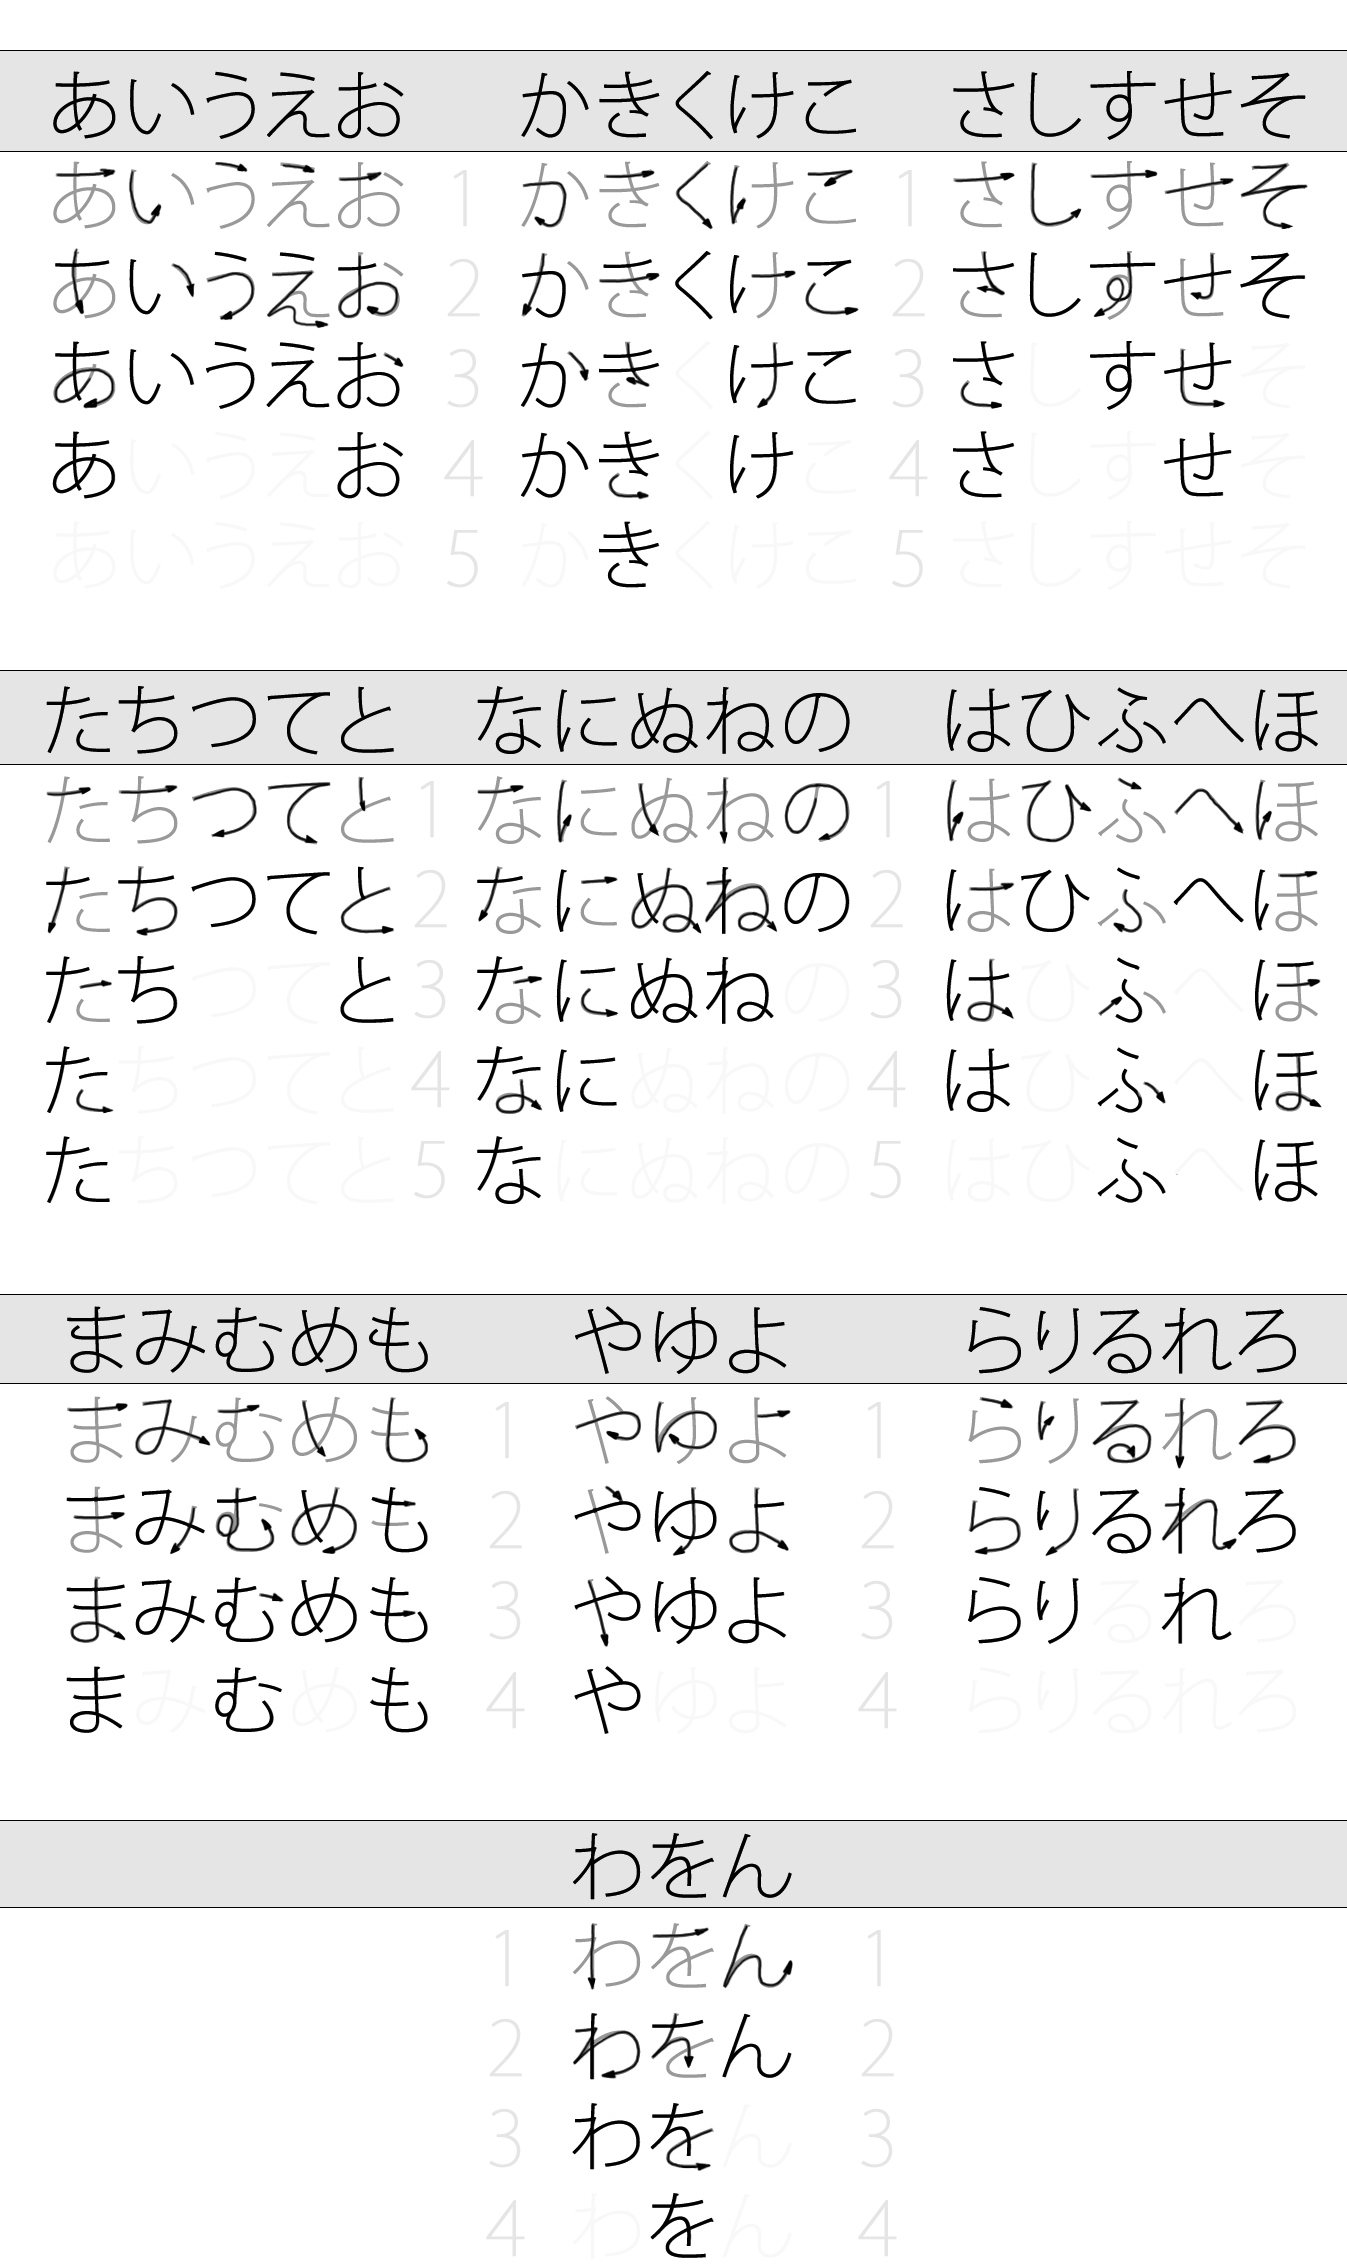
\includegraphics{../data/media/hiraganastrokes.jpg}}\nopagebreak[4]\par {\smaller \smaller Stroke diagrams for hiragana}\end{center}



\vspace{0.5em}
\begin{center}
\fbox{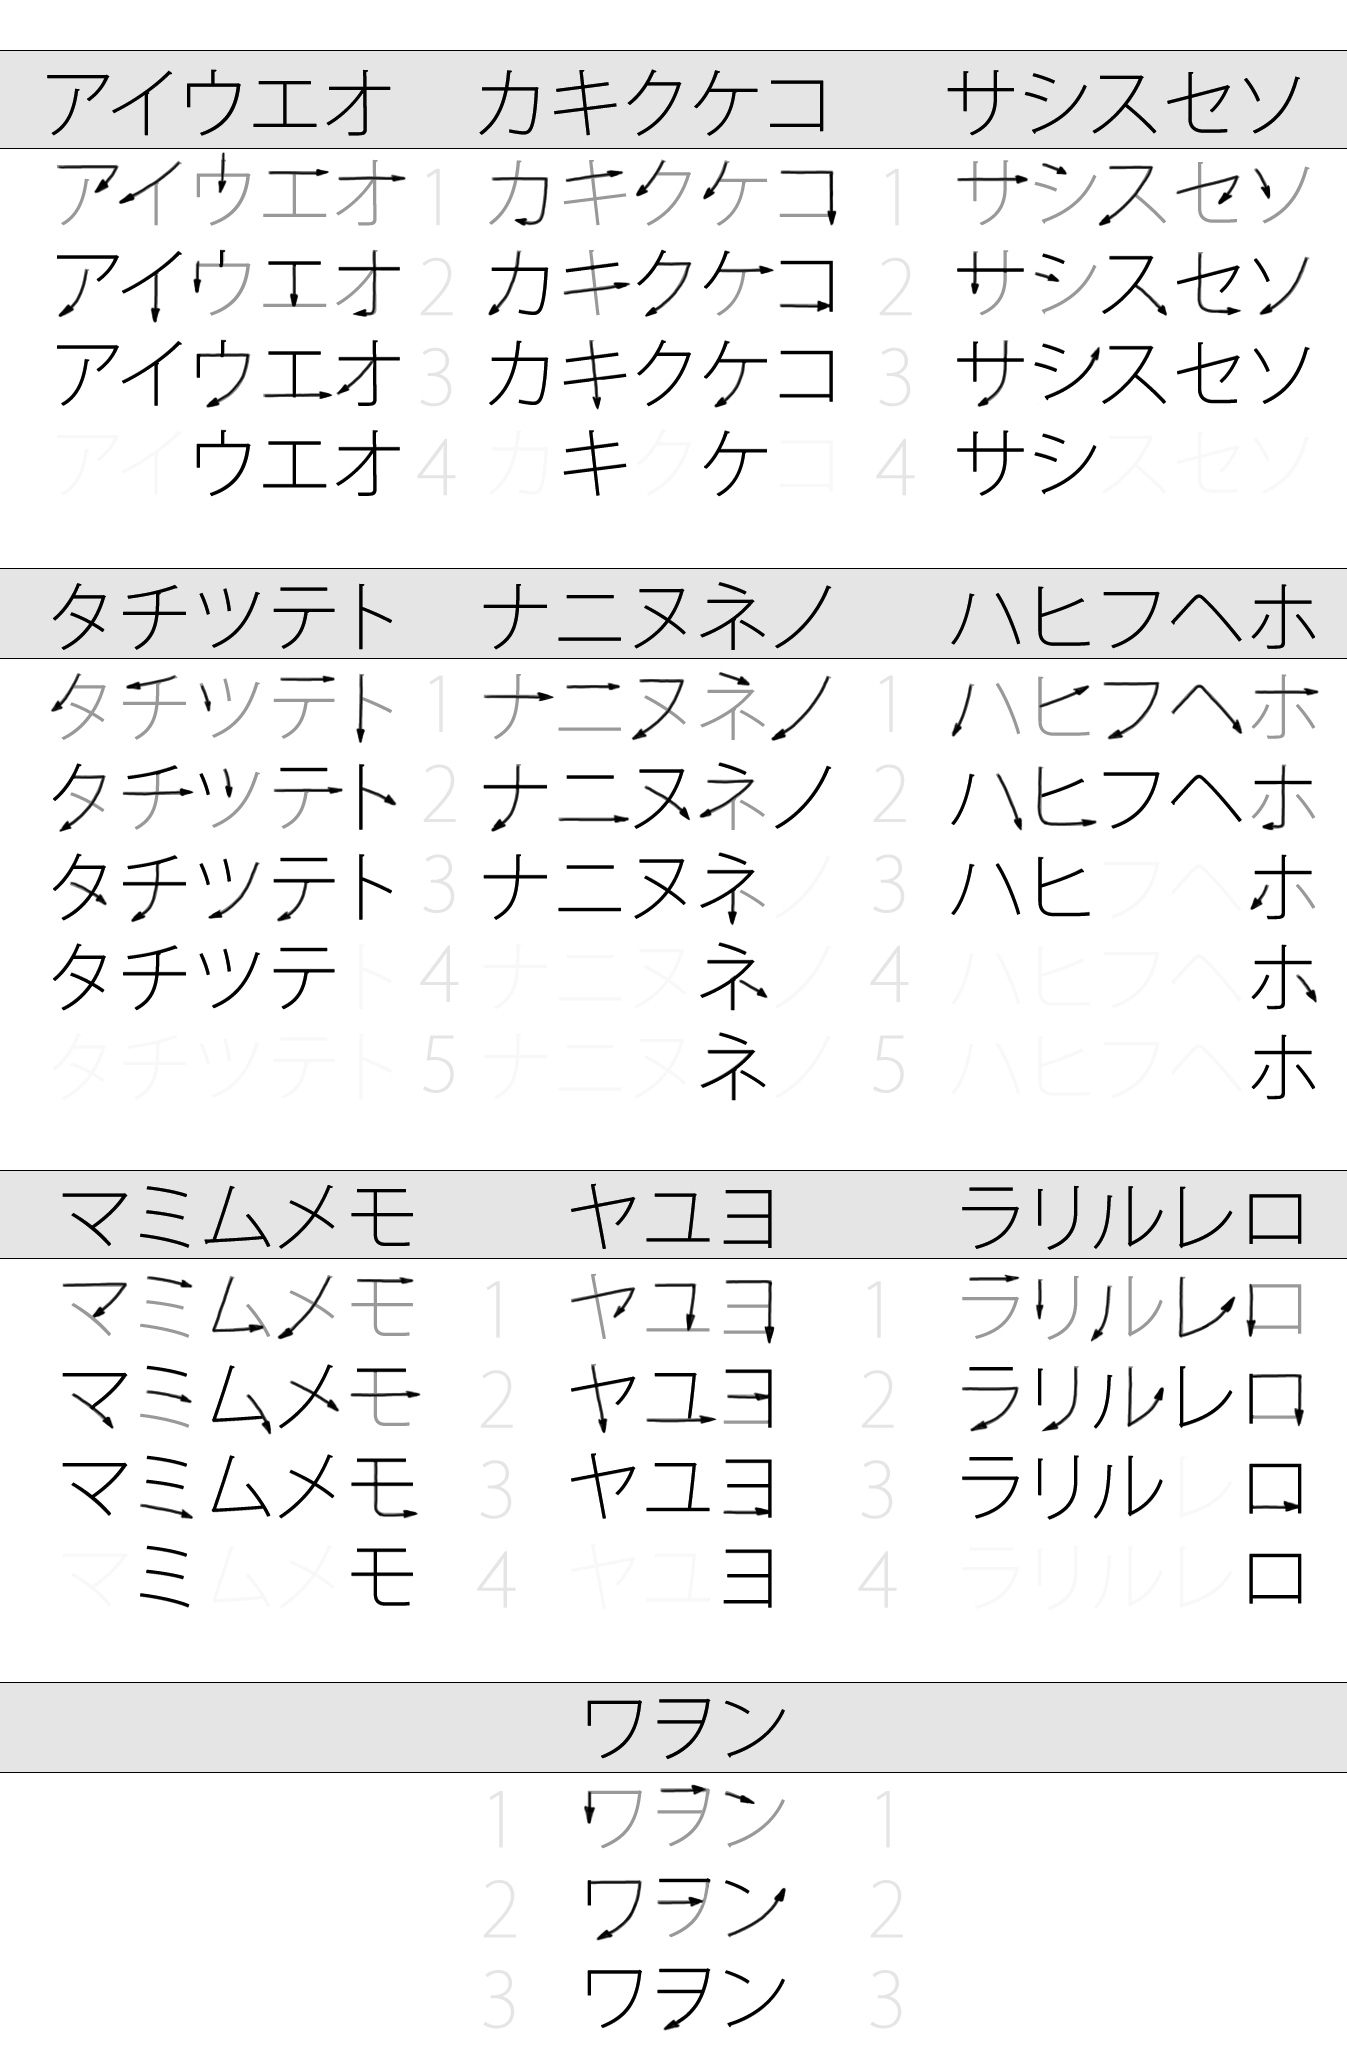
\includegraphics{../data/media/katakanastrokes.jpg}}\nopagebreak[4]\par {\smaller \smaller Stroke diagrams for katakana}\end{center}


\subsection{Pronouncing Japanese}

\index[english]{Pronunciation}Pronunciation wise‚ each of these syllables is equally long. This is traditionally explained by referring to the pronunciation of Japanese as \index[english]{Mora}mora‚ a linguistic term meaning “the time required to pronounce an ordinary or normal short sound or syllable”. In Japan‚ this concept of mora is usually explained with the easier concept of \index[english]{Drum beat}drum beats: each basic syllable is one beat long‚ with certain combinations of kana lasting one and a half or two beats.

The vowel sounds of Japanese‚ あ‚ い‚ う‚ え and お do not all have English equivalents; あ is actually identical to the initial vowel sound in “I” or “eye” — that is‚ the ‘a’ sound without the finalising ‘i’ sound. The い is a little easier‚ sounding like the ‘ee’ in ‘creep’. The う is particularly annoying‚ because there is no English equivalent. It is identical to the vowel sounds of properly Scottish ‘you’ or ‘do’‚ or the Dutch open ‘u’ such as in ‘huren’. え is pronounced like in the English ‘help’‚ and the お‚ finally‚ is pronounced like the ‘o’ in ‘or’.

While for most kana the \index[english]{Consonant}consonant sound is reasonably approximated by the transcribed consonant as listed in the earlier tables‚ there are a few notable exceptions. For instance‚ while romanised as “hi”‚ ひ/ヒ is usually pronounced with a consonant that doesn’t sound like an ‘h’‚ but more like the German or Scottish “ch” as found in German words such as “ich” (meaning “I”) and Scottish words such as “loch” (meaning “lake”).

Also in the は-column‚ the syllable ふ/フ does not have an ‘h’ as consonant sound‚ or even the ‘f’ consonant sound that it is typically transcribed with‚ but rather uses only pure \index[english]{Aspiration}aspiration as initial sound. This is mostly unknown in western languages‚ and will be the hardest to get right for people starting out with Japanese. Rather than being formed in the mouth‚ the syllable ふ starts being formed at the \index[english]{Diaphragm}diaphragm‚ while breathing out. Paired with the lips shaped as if casually blowing out a match or candle (rather than tightened for whistling)‚ this rush of air is then given a vowel sound‚ and the syllable is complete.

In the つ—column we also see an interesting pronunciation ‘quirk’: while ち and つ‚ strictly speaking‚ have voiced versions‚ written ぢ and づ‚ over the years the difference in pronunciation between ぢ and じ‚ and づ and ず‚ has all but disappeared‚ leading to an official move towards replacing these ぢ and づ with じ and ず entirely. However‚ there are (quite a number of) exceptions to this move for replacement: if the two first kana of a word are the same‚ but the second one is voiced‚ the same kana are used (for example‚ つづく and ちぢめる). Also‚ in compound words in which voicing occurs‚ the original kana form is used (for instance‚ \ruby{片}{かた} + \ruby{付}{つ}く → \ruby{片付}{かたづ}く and \ruby{鼻}{はな} + \ruby{血}{ち} → \ruby{鼻血}{はなぢ}). This exception only applies when the compound word can be considered a combination of words. Both 片付く and 鼻血 derive their meaning from their constituent words‚ but in a word like \ruby{稲妻}{いなずま}‚ meaning “lightning”‚ the first kanji refers to rice plants‚ and the second kanji refers to (someone’s) wife. In these words‚ even if the affixed compound would normally have a つ or ち‚ the voicing is written as ず or じ in modern Japanese‚ rather than づ or ぢ.

That said‚ voicing in compound nouns is a bit strange in that there are no rules to tell when something will‚ or will not voice‚ so the best strategy — which applies to learning words in general anyway — is to learn words as word first‚ then learn them as combinations‚ rather than the other way around.

Finally‚ the ら—column can be a problem because for most western listeners‚ different people will seem to pronounce the initial consonant in this column differently. While in many western languages the consonants “d”‚ “l”‚ and “r” are considered quite distinct‚ in Japanese this distinction is far less; any syllable starting with a consonant ranging from a full fledged “l” to a rolling Spanish “r” will be interpreted as a syllable from the ら—column‚ with the “standard” pronunciation being somewhere between a “d” and an “r”.

\subsubsection{Not pronouncing Japanese}

This sounds like an oddly named section‚ but some bits in written Japanese are actually not really pronounced at all. In fact‚ not infrequently you will hear Japanese that does not seem to reflect the written form‚ with the verb “desu” seemingly being pronounced “des”‚ the adjective “hayaku” seemingly being pronounced “hayak”‚ the command “shiro” seemingly being pronounced “sh’ro”‚ and many more of such vocal omissions.

In fact‚ many syllables with an い— or う—sound tend to have these vowel sounds left almost unpronounced. I say almost‚ because the vowel sound is typically preserved by virtue of the consonants used. For instance‚ the word そして‚ transcribed as ‘soshite’ is typically pronounced in such a way that it can be considered transcribable as “sosh’te” instead. However‚ forming “sh” means also forming a pseudo-vowel sound. In fact‚ even in this “omitted vowel” there is room for variation‚ so that a “sh” can sound like it was supposed to become “shi” or “shu”‚ and it is this feature that is exploited quite heavily in Japanese.

This leads to a small problem. Because it sounds like the vowel is entirely missing‚ you might be tempted to mimic this sound‚ but end up genuinely omitting the vowel entirely because that’s what your ears — which are not yet accustomed to Japanese phonetics — think is happening. However‚ this also makes your Japanese highly unnatural‚ because to a Japanese ear the vowel is only mostly omitted‚ not entirely.

The problem then is one of hearing: when learning a new language it is important to “unlearn” how to hear language. Much like how we have learned to see the world in a way that it’s actually not (you will consider a brown table with a light shining on one end‚ brown‚ instead of brown on one end‚ and a completely different colour where the light is hitting it)‚ as infants we learn to disregard any and all sounds that don’t feature in the languages we’re raised with. As such‚ remarkable as this may sound‚ we unlearn how to hear things accurately‚ and instead learn how to map what we hear to what we know the language is supposed to sound like. While highly effective when learning a language‚ or a family of languages with similar pronunciations‚ it’s disastrous when learning a language that has a different phonetic system.

The best advice with regards to this is to simply listen to a lot of Japanese. It takes time and effort to unlearn the unconscious mapping your brain does for you. You’re going to get it wrong‚ but as long as you know you are‚ you’ll be on the right track.

\subsection{Hiragana and katakana differences}

If hiragana and katakana sound exactly the same‚ why then are there two different scripts?

When the Japanese first developed a written system‚ it was based on the characters used in China for the Chinese language‚ in which for the most part the meaning of the characters were subservient to what they sounded like: if a word had an “a” sound in it‚ then any \index[english]{Chinese characters}Chinese character that sounded like “a” could be used for it‚ without any real regard for its meaning. This “using certain characters for their sound only” became more widespread as the number of characters per syllable dropped from quite many to only a handful‚ and as writing became more widespread two \index[english]{Syllabic script}syllabic scripts developed. One‚ which simplified \index[english]{Phonetic kanji}phonetic kanji by omitting parts of them lead to what is today called \index[english]{Kana!katakana}katakana. Another‚ which simplified phonetic kanji by further and further reducing the complexity of the cursive forms for these kanji‚ has become what is known today as \index[english]{Kana!hiragana}hiragana. We can see this illustrated in the next figure‚ which shows the characters the hiragana came from‚ and the highly stylistic cursive form characters had‚ highlighting the degree of simplification that cursive writing brought with it.


\vspace{0.5em}
\begin{center}
\fbox{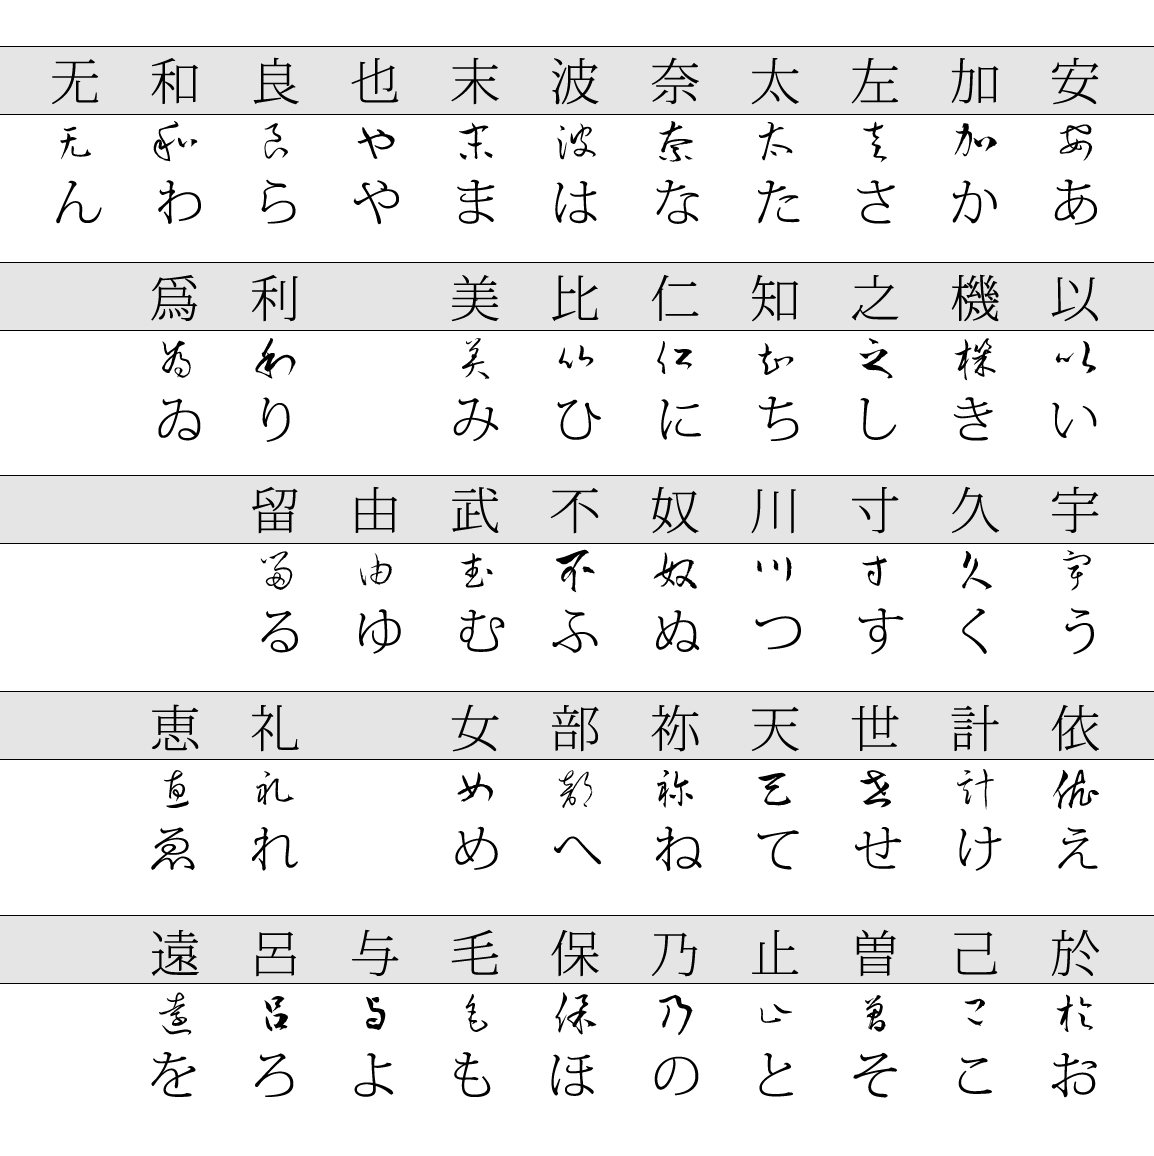
\includegraphics{../data/media/hiraganaderivation.jpg}}\nopagebreak[4]\par {\smaller \smaller The hiragana derivations from cursive script}\end{center}


Katakana got a slightly different treatment‚ in that these are actually fragments of characters‚ rather than stylistic simplifications. The second derivations figure illustrates this‚ with a note that the fragments were lifted from handwritten characters‚ so that the “logic” is mostly found in the cursive line of characters.

These two scripts have differed in roles throughout history‚ and in modern Japanese hiragana is used for anything Japanese that does not use (or need) kanji‚ and katakana is used in the same way that we use italics in western language‚ as well as for words that have been imported into Japanese from other languages over the course of history. The only genuine difference between the two scripts is the way in which long vowel sounds are written‚ as we shall see in the next section.


\vspace{0.5em}
\begin{center}
\fbox{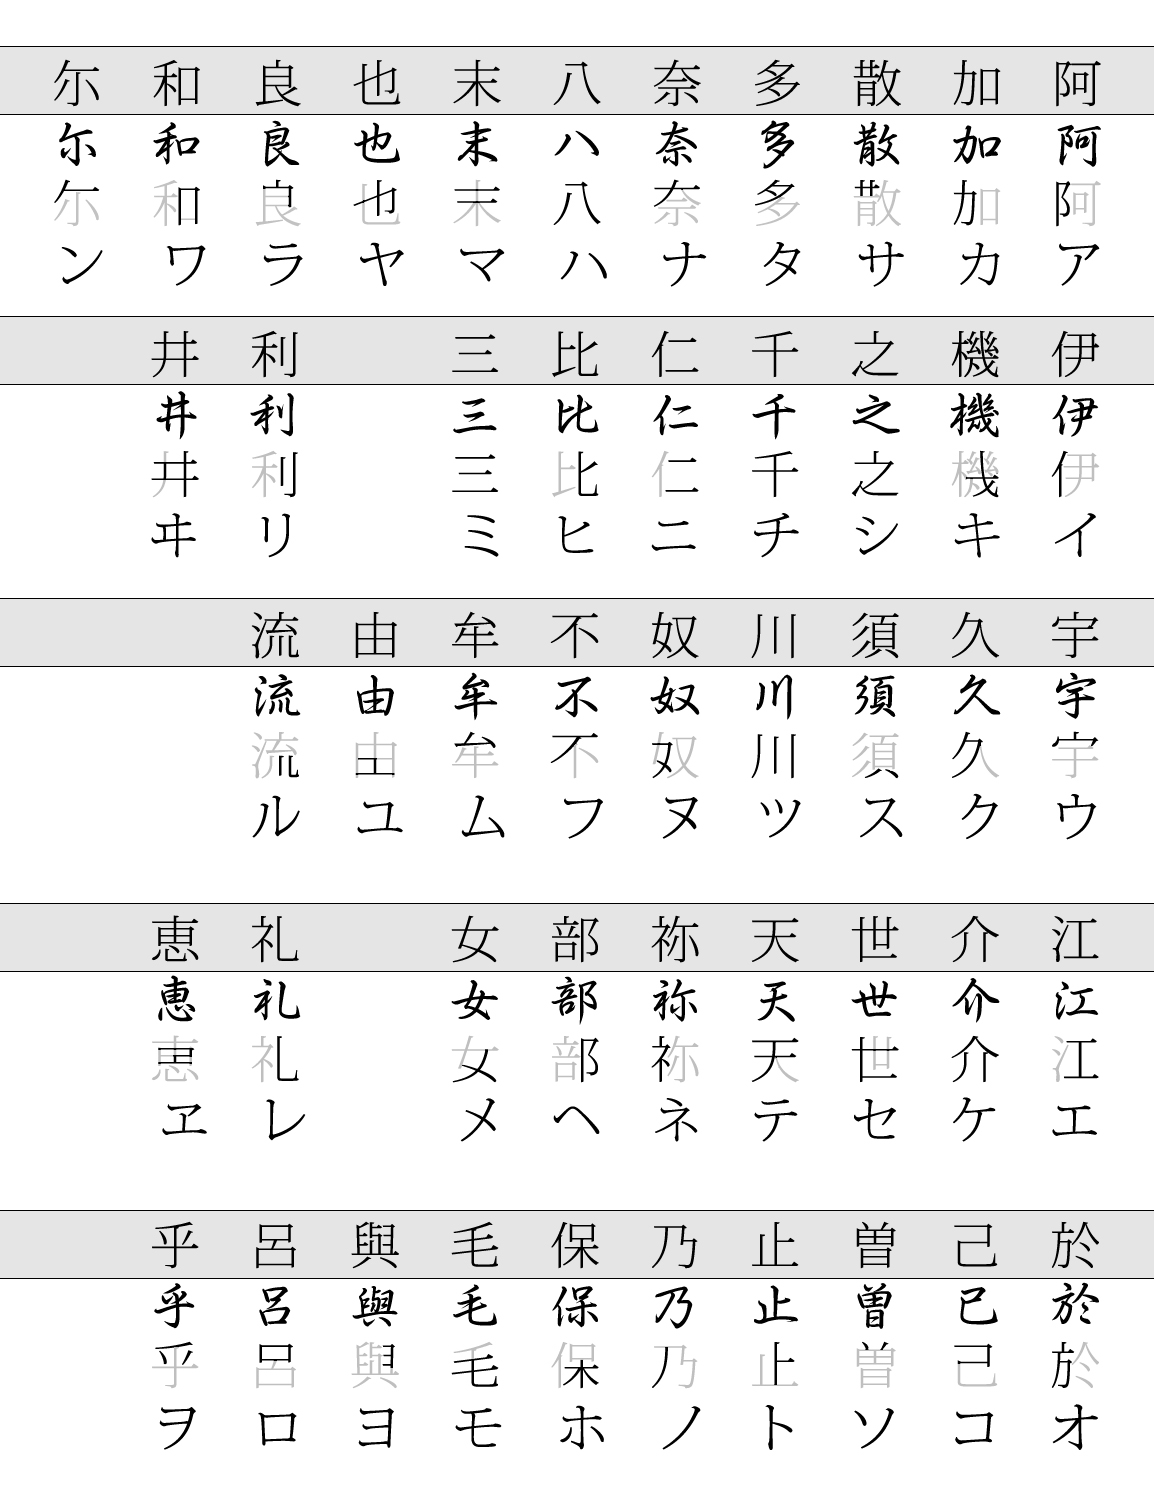
\includegraphics{../data/media/katakanaderivation.jpg}}\nopagebreak[4]\par {\smaller \smaller The katakana derivations}\end{center}



\section{Writing spoken Japanese}

Using the kana as basic building blocks‚ Japanese pronunciation consists of a few more things beyond basic syllables: in addition to “simple” syllable sounds‚ it contains \index[english]{Long vowel}long vowels‚ \index[english]{Glide}glides and \index[english]{Double consonant}double consonants.

\index[english]{Long vowel}Long vowels‚ contrary to the name‚ do not always mean “the same vowel‚ twice as long”. Strictly speaking‚ a long vowel in Japanese is a combination of two vowels‚ pronounced over two “\index[english]{Drum beat}drum beats”. In katakana‚ long vowels are really just that‚ a vowel with a dash to indicate the sound has been doubled in length‚ but in hiragana the doubling is different. Of the five basic Japanese vowel sounds (あ‚ い‚ う‚ え and お) the first three have fairly simple long vowel counterparts in hiragana‚ simply doubling in writing‚ but the latter two are more complicated‚ having two different written forms:

\vspace{0.5cm}
\smaller
\begin{mytabular}{| l  l  l |}\hline 
\rule{0pt}{2.4ex} & hiragana & katakana\\ 
\hline
\rule{0pt}{2.4ex}あ & ああ & アー\\ 
\rule{0pt}{2.4ex}い & いい & イー\\ 
\rule{0pt}{2.4ex}う & うう & ウー\\ 
\rule{0pt}{2.4ex}え & ええ‚ えい & エー\\ 
\rule{0pt}{2.4ex}お & おお‚ おう & オー\\ 
\hline 
\end{mytabular}
\larger
\vspace{0.5cm}


While the pronunciation for ああ‚ いい and うう are intuitive (same sound‚ twice as long)‚ the pronunciations for ええ‚ えい‚ おお and おう and more subtle. The first‚ ええ‚ may be pronounced as a “same sound‚ twice as long” え‚ but may also be pronounced as えい‚ which is similar to the ‘-ay’ in the English ‘hay’. For おお‚ the pronunciation is like “oa” in “oak”‚ with おう often sounding the same‚ but when pronounced slowly‚ having a distinct hint of “u” at the end.

This doubling is the same for syllables with consonant sounds‚ so that for instance vowel doubling for the syllables from the ま—column look as follows:

\vspace{0.5cm}
\smaller
\begin{mytabular}{| l  l  l |}\hline 
\rule{0pt}{2.4ex} & hiragana & katakana\\ 
\hline
\rule{0pt}{2.4ex}あ & まあ & マー\\ 
\rule{0pt}{2.4ex}い & みい & ミー\\ 
\rule{0pt}{2.4ex}う & むう & ムー\\ 
\rule{0pt}{2.4ex}え & めえ‚ めい & メー\\ 
\rule{0pt}{2.4ex}お & もお‚ もう & モー\\ 
\hline 
\end{mytabular}
\larger
\vspace{0.5cm}


In addition to long vowels‚ Japanese words may contain “\index[english]{Glide}glides”. Being considered \glslink{contraction}{contractions} of い—row syllables with any one of the three syllables や‚ ゆ and よ‚ glides are written as the い—row syllable‚ normal sized‚ and then the や‚ ゆ or よ syllable at either half height (for horizontally written Japanese) or half width (for vertically written Japanese). To illustrate:

\vspace{0.5cm}
\smaller
\setlength\LTleft\parindent
\setlength\LTright\fill
\Needspace{6\baselineskip}
\begin{longtable}[h]{| l  l  l  l  l  l |}\hline
\rule{0pt}{2.4ex} & kana & pronunciation &  & as glide & pronunciation\\ 
\hline 
\endfirsthead
\hline
\rule{0pt}{2.4ex} & kana & pronunciation &  & as glide & pronunciation\\ 
\hline 
\endhead
\hline
\endfoot
\hline
\endlastfoot
\rule{0pt}{2.4ex}き + や & きや & kiya &  & きゃ & kya\\ 
\rule{0pt}{2.4ex}し + ゆ & しゆ & shiyu &  & しゅ & shu\\ 
\rule{0pt}{2.4ex}ち + よ & ちよ & chiyo &  & ちょ & cho\\ 
\rule{0pt}{2.4ex}み + や & みや & miya &  & みゃ & mya\\ 
\rule{0pt}{2.4ex}ひ + よ & ひよ & hiyo &  & ひょ & hyo\\ 
\rule{0pt}{2.4ex}に + ゆ & にゆ & niyu &  & にゅ & nyu\\ 
\rule{0pt}{2.4ex}り + よ & りよ & riyo &  & りょ & ryo\\ 
\end{longtable}
\larger
\vspace{0.5cm}


While a written combination of two syllables‚ the glide it represents is only a single “\index[english]{Drum beat}drum beat” long‚ just as the regular syllables. Thus‚ the word キャンプ is three beats long: spelled out‚ it will be pronounced きゃ‚ ん and ぷ.

Finally‚ the last feature of spoken Japanese reflected in writing is what is known as the “\index[english]{Double consonant}double consonant”: a reasonably recent change to the way Japanese is written (in the sense that this change occurred sometime during the medieval period‚ when written Japanese had been around for a little under a millennium) which indicates that a particular consonant has a short pause before it is actually pronounced. This consonant doubling is found in a number of western languages as well‚ such as in Italian‚ where words like ‘tutti’ have a written double consonant while in terms of pronunciation there is simply a pause before the consonant. In Japanese‚ because there are no actual ‘loose’ consonants‚ the doubling is represented by a special character: a つ (or ツ) written either half height (in horizontal writing) or half width (in vertical writing) to indicate the pause. To illustrate the difference between this small つ/ツ and the regular form‚ a few example words:

\vspace{0.5cm}
\smaller
\begin{mytabular}{| l  l  l |}\hline 
\rule{0pt}{2.4ex}small っ & pronunciation & meaning\\ 
\hline
\rule{0pt}{2.4ex}はっか & “hakka” & ignition\\ 
\rule{0pt}{2.4ex}しっけ & “shikke” & humidity\\ 
\rule{0pt}{2.4ex}まっか & “makka” & intensely red\\ 
\hline 
\end{mytabular}
\larger
\vspace{0.5cm}

\smaller
\begin{mytabular}{| l  l  l |}\hline 
\rule{0pt}{2.4ex}normal つ & pronunciation & meaning\\ 
\hline
\rule{0pt}{2.4ex}はつか & “hatsuka” & 20 days/20\textsuperscript{th} day\\ 
\rule{0pt}{2.4ex}しつけ & “shitsuke” & upbringing\\ 
\rule{0pt}{2.4ex}まつか & “matsuka” & the ‘Pine’ family of trees\\ 
\hline 
\end{mytabular}
\larger
\vspace{0.5cm}


This “つ/ツ as a pause” is also applied when a \index[english]{Glottal stop}\glslink{glottal stop}{glottal stop} is needed in for instance an exclamation‚ “あっ!”‚ which is an exclamation with a “cut off” rather than long vowel sound.

\subsection{Katakana specific}

As \index[english]{Kana!katakana}katakana has been used to write out words imported from other languages into Japanese‚ it has a few extra “rules” that do not apply to written hiragana‚ including a number of ways to produce normally \index[english]{“illegal” syllables}“illegal” syllables: syllables that do not fit in the Japanese table of syllables‚ but are found in foreign words nonetheless. Examples of these are for instance the initial syllable “fi” in the English word “fire”‚ or the “swe” in “Sweden”.

The table of approximating writing is as follows‚ observing English pronunciation rules (combinations with normal Japanese orthography are omitted):

\vspace{0.5cm}
\smaller
\setlength\LTleft\parindent
\setlength\LTright\fill
\Needspace{6\baselineskip}
\begin{longtable}[h]{| l  l  l  l  l  l |}\hline
\rule{0pt}{2.4ex} & a & e & i & o & u\\ 
\hline 
\endfirsthead
\hline
\rule{0pt}{2.4ex} & a & e & i & o & u\\ 
\hline 
\endhead
\hline
\endfoot
\hline
\endlastfoot
\rule{0pt}{2.4ex}ch &  & チェ\\ 
\rule{0pt}{2.4ex}d &  &  & ディ &  & ドゥ\\ 
\rule{0pt}{2.4ex}f & ファ & フェ & フィ & フォ\\ 
\rule{0pt}{2.4ex}fj/fy &  &  &  &  & フィウ\\ 
\rule{0pt}{2.4ex}j &  & ジェ\\ 
\rule{0pt}{2.4ex}q & クァ & クェ & クィ & クォ & ク\\ 
\rule{0pt}{2.4ex}s &  &  & セィ\\ 
\rule{0pt}{2.4ex}sh &  & シェ\\ 
\rule{0pt}{2.4ex}sw & スァ & スェ & スィ & スォ & スゥ\\ 
\rule{0pt}{2.4ex}t &  &  & ティ &  & トゥ\\ 
\rule{0pt}{2.4ex}v (1) & ヴァ & ヴェ & ヴィ & ヴォ & ヴ\\ 
\rule{0pt}{2.4ex}w &  & ウェ & ウィ & ウォ & ウ\\ 
\rule{0pt}{2.4ex}x & ックサ & ックセ & ックセィ & ックソ & ックス\\ 
\rule{0pt}{2.4ex}y &  & イェ & イ\\ 
\rule{0pt}{2.4ex}z &  &  & ゼィ\\ 
\end{longtable}
\larger
\vspace{0.5cm}


Note that ‘wo’ is not ヲ (as that is pronounced お)‚ and that for the ‘x’ series‚ the leading ッ is the consonant doubling symbol.

In addition to these‚ there are also a number of consonants which‚ in terms of pronunciation‚ already have Japanese counterparts:

\vspace{0.5cm}
\smaller
\begin{center}
\begin{mytabularcentered}{| l  l |}\hline 
\rule{0pt}{2.4ex}consonant & column\\ 
\hline
\rule{0pt}{2.4ex}c‚ pronounced as ‘s’ & uses the さ—column\\ 
\rule{0pt}{2.4ex}c‚ pronounced as ‘k’ & uses the か—column\\ 
\rule{0pt}{2.4ex}l & uses the ら—column\\ 
\rule{0pt}{2.4ex}v (2) & uses the ば—column. Preferred to ‘v (1)’ in the above table.\\ 
\hline 
\end{mytabularcentered}
\end{center}
\larger
\vspace{0.5cm}


Due to the fact that most \index[english]{Loan words}loan words have come from some specific language‚ many of which are not English‚ Japanese loan words may have a different written form than expected. For instance‚ Brussels is written as ブリュッセル‚ “buryusseru”‚ rather than ブラセルズ‚ “buraseruzu”‚ and English (the people) is written as イギリス‚ “igirisu”‚ rather than イングリッシュ‚ “ingurisshu”.

\subsection{\index[english]{Punctuation}Punctuation and writing}

Of course‚ in addition to a “letter” script‚ there is \index[english]{Interpunction}\glslink{interpunction}{interpunction} — symbols that indicate pauses‚ stops‚ quotes and other such things. In Japanese‚ the following \glslink{punctuation}{punctuation} symbols are common:

\vspace{0.5cm}
\smaller
\setlength\LTleft\fill
\setlength\LTright\fill
\Needspace{6\baselineskip}
\begin{longtable}[h]{| l  l |}\hline
\rule{0pt}{2.4ex} & symbol\\ 
\hline 
\endfirsthead
\hline
\rule{0pt}{2.4ex} & symbol\\ 
\hline 
\endhead
\hline
\endfoot
\hline
\endlastfoot
\rule{0pt}{2.4ex}\index[english]{Interpunction!full stop}full stop & 。\\ 
\rule{0pt}{2.4ex}\index[english]{Interpunction!comma}comma & 、\\ 
\rule{0pt}{2.4ex}\index[english]{Interpunction!single quote}single quotes & 「 and 」\\ 
\rule{0pt}{2.4ex}\index[english]{Interpunction!double quote}double quotes & 『 and 』\\ 
\rule{0pt}{2.4ex}\index[english]{Interpunction!parentheses}parentheses & （ and ）\\ 
\rule{0pt}{2.4ex}\index[english]{Interpunction!kanji repeater}kanji repeater & 々\\ 
\rule{0pt}{2.4ex}\index[english]{Interpunction!separator}separators & ・ and ＝\\ 
\rule{0pt}{2.4ex}\index[english]{Interpunction!drawn sound}drawn sound & ～\\ 
\rule{0pt}{2.4ex}\index[english]{Interpunction!ellipsis}ellipsis & … (usually written twice: ……)\\ 
\end{longtable}
\larger
\vspace{0.5cm}


Less used‚ but always good to have seen are the following:

\vspace{0.5cm}
\smaller
\begin{center}
\begin{mytabularcentered}{| l  l |}\hline 
\rule{0pt}{2.4ex} & symbol\\ 
\hline
\rule{0pt}{2.4ex}\index[english]{Interpunction!idem dito}idem dito & 〃\\ 
\rule{0pt}{2.4ex}\index[english]{Interpunction!hiragana repeater}hiragana repeaters & ゝ‚ ゞ\\ 
\rule{0pt}{2.4ex}\index[english]{Interpunction!katakana repeater}katakana repeaters & ヽ‚ ヾ\\ 
\rule{0pt}{2.4ex}kanji \index[english]{Interpunction!closing mark}closing mark & 〆\\ 
\hline 
\end{mytabularcentered}
\end{center}
\larger
\vspace{0.5cm}


And then there are western \index[english]{Punctuation}punctuations which have Japanese counterparts‚ but tend to be expressed differently instead:

The symbol ? is written the same way as in English‚ but typically the particle か is used instead. This particle か serves both as \index[english]{Interpunction!question mark}question mark‚ as well as a marker for parts of a sentences‚ indicating they are questioning instead of stating. Similarly‚ the symbol ! is written the same way as in English‚ but typically \index[english]{Interpunction!exclamation}exclamations are simply avoided. Instead‚ emphasis particles such as よ or わ may be used for effect‚ but these do not signify real exclamation.

Finally‚ not quite interpunction but important nonetheless are the two ways to emphasise parts of written language in the same way we use \index[english]{Bold}bold or \index[english]{Underlining}underlining in western composition: \index[english]{Interpunction!dotting}dotting and \index[english]{Interpunction!lining}lining. In horizontal writing‚ words will have dots over each syllable or kanji‚ or a line over the entire emphasised section. In vertical writing‚ the dots and lining is placed on the right side of text.

In addition to knowing the basics about which symbols can be used‚ Japanese (as well as some other Asian languages such as Chinese) has the unique problem of deciding in which direction to write. For all its modernising‚ some things such as \index[english]{Writing!direction}writing remain unchanged. As such‚ for the most part printed Japanese (as well as handwritten material) is written top down‚ right to left. In contrast‚ most Japanese material on the internet is typically written in a western fashion‚ with the text running left to right‚ top to bottom.

To make matters more interesting‚ in recent history‚ Japanese could also be written horizontally right-to-left. This practice has pretty much disappeared except in shipping (ship names may still be written in this way) and for ‘older style’ shop signs. You will not encounter full texts written in this way in modern or even just post-Meiji older Japanese.

There are a few differences between horizontal and vertical writing‚ most notably in terms of where to place half size characters and interpunction:

\vspace{0.5cm}
\smaller
\setlength\LTleft\fill
\setlength\LTright\fill
\Needspace{6\baselineskip}
\begin{longtable}[h]{| l  l  l |}\hline
\rule{0pt}{2.4ex} & horizontal & vertical\\ 
\hline 
\endfirsthead
\hline
\rule{0pt}{2.4ex} & horizontal & vertical\\ 
\hline 
\endhead
\hline
\endfoot
\hline
\endlastfoot
\rule{0pt}{2.4ex}half size characters & \index[english]{Writing!half-height}half-height & \index[english]{Writing!half-width}half-width‚ right aligned\\ 
\rule{0pt}{2.4ex}comma‚ full stop & lower left: [、]‚ [。] & upper-right: [︑]‚ [︒]\\ 
\rule{0pt}{2.4ex}opening quotes & corner in the upper left (「) & corner in the upper right (﹁)\\ 
\rule{0pt}{2.4ex}closing quotes & corner in the lower right (」) & corner in the lower left (﹂)\\ 
\rule{0pt}{2.4ex}parentheses & left and right: i.e. ( and ) & above and below: i.e. ⁀ and ‿\\ 
\rule{0pt}{2.4ex}dotting & above characters & to the right of characters\\ 
\rule{0pt}{2.4ex}lining & above characters & to the right of characters\\ 
\rule{0pt}{2.4ex}drawn sound‚ hyphen & horizontal (〰‚ ―) & vertical ( ︴‚︱)\\ 
\rule{0pt}{2.4ex}ellipsis & horizontal (…) & vertical (⁝)\\ 
\end{longtable}
\larger
\section{Kanji}


One of written Japanese’s most well-known features is that it comprises three writing systems: the two kana scripts‚ and a third script called \index[english]{Kanji}kanji‚ translating as “\index[english]{Chinese characters}Chinese characters”‚ which are \index[english]{Ideograph}ideographs that over the course of history made their way from China to Japan. One of the biggest problems with kanji is that there aren’t just many‚ but each one can have a multitude of \index[english]{Pronunciation}pronunciations dependent on which words the kanji is being used for. To look at why this is‚ a brief history of how modern Japanese got the kanji that are used today is in order.

Early Japanese evolved as a purely spoken language. Without a written form‚ indeed seemingly without having discovered writing at all‚ the first instances of writing in Japan were in fact not Japanese at all‚ but Chinese: after having come into contact with the Chinese and their intricate writing system‚ writing in early Japan (circa the late sixth century) was restricted to immigrant scribes‚ who wrote official records in \index[english]{Classical!Chinese}classical Chinese. While initially a rarity‚ the \index[english]{Taika reform}Taika reform of the mid-seventh century changed all that.

Reforming Japan to a more Chinese-inspired state‚ based on centralisation of government and Confucian philosophy‚ the need for a state clergy transformed the largely illiterate Japanese society to one with literacy as an essential part of court and intellectual life. The prestigious rank of scribe became a hereditary rank‚ and so as generations of scribes came and went‚ the Chinese that was used slowly drifted away from proper Chinese‚ and more towards a \index[english]{Hybrid writing style}hybrid style of Chinese and the form of Japanese as it was used at the time. However‚ the readings used for Chinese characters were more or less fixed‚ and the readings that survive from that period are known today as \index[japanese]{Kanji readings!ごおん (呉音)}\ruby{呉音}{ごおん}‚ \index[english]{Kanji readings!go’on}go’on‚ readings.

Then‚ in the seventh and eighth century‚ during the Chinese \index[english]{Tang dynasty}Tang dynasty‚ there was another cultural exchange between Japan and China‚ leading to a second influx of readings for Chinese characters. As China changed rulers‚ so too did the dominant dialect for the Chinese language‚ and the readings that were brought back to Japan from this second exchange were in some cases radically different from the initial readings the Japanese had become familiar with. Readings for kanji from this period are known as \index[japanese]{Kanji readings!かんおん (漢音)}\ruby{漢音}{かんおん}‚ \index[english]{Kanji readings!kan’on}kan’on‚ readings.

Finally‚ in the fourteenth century‚ during the most famous of Chinese dynasties — the \index[english]{Ming Dynasty}Ming Dynasty — there was another influx of Chinese. This influx came from two fronts: firstly‚ the merchants doing business with the Chinese brought back home readings that are referred to as \index[japanese]{Kanji readings!とうおん (唐音)}\ruby{唐音}{とうおん}‚ \index[english]{Kanji readings!tō’on}tō’on‚ and secondly from Zen monks who went to study \index[english]{Zen Buddhism}Zen Buddhism in China and brought back readings that are referred to as \index[japanese]{Kanji readings!そうおん (宋音)}\ruby{宋音}{そうおん}‚ \index[english]{Kanji readings!sō’on}sō’on. Rather than a single exchange‚ this was an ongoing effort‚ and so 唐音 readings tend to span from the late thirteenth century to well into the \index[english]{Edo period}Edo period (\index[japanese]{えどじだい (江戸時代)}\ruby{江戸時代}{えどじだい}‚ \index[english]{Edojidai}edojidai)‚ also known as the \index[english]{Tokugawa period}Tokugawa period (\index[japanese]{とくがわじだい (徳川時代)}\ruby{徳川時代}{とくがわじだい}‚ \index[english]{Tokugawajidai}tokugawajidai)‚ named after the first Edo shogun Tokugawa Ieyasu (\ruby{徳川}{とくがわ}\ruby{家康}{いえやす})‚ which lasted until the late nineteenth century.

The naming for these readings‚ however‚ can be slightly confusing. 呉音 readings are known as \index[english]{Kanji readings!“wu” readings}“wu” readings. However‚ this name does not refer to the Wu dynasty (which spans the first two centuries a.d.) but simply to the region the readings are believed to have come from (呉 being the name of the Wu region in Jiangnan‚ 江南‚ in modern China). The 漢音 readings are called \index[english]{Kanji readings!“han” readings}“han” readings‚ but have essentially nothing to do with the Han Dynasty‚ which spanned the late third century BCE.

The 唐音 readings‚ equally confusing‚ are referred to as Tang readings‚ even though this name would be more appropriate for the 漢音 readings‚ which actually derive from Tang Chinese. Rather‚ 唐音 derive their readings from Chinese as it was used during the Sung dynasty and onward.

In addition to these changes to Chinese readings‚ the written language itself slowly moved away from Chinese proper‚ through a Chinese-Japanese hybrid written language‚ to what is essentially the Japanese we know today: mixed Chinese characters with \index[english]{Syllabic script}syllabic script (itself derived from Chinese characters being used phonetically) with different readings for Chinese characters typically indicating different interpretations of the characters used.

While there had been no written language before the introduction of Chinese‚ there had certainly been a language‚ which survived throughout the ages by virtue of the commoners not needing to bother with writing‚ and thus not incorporating Chinese into their language as much as royals and officials would. This eventually led to native Japanese pronunciation being applied to written Chinese‚ giving us two different reading “systems”: the \index[japanese]{おんよみ (音読み)}\ruby{音読}{おんよ}み‚ “\index[english]{On’yomi}on’yomi”‚ which are the \index[english]{Kanji readings!Chinese derived readings}Chinese derived readings‚ and the \index[japanese]{くんよみ (訓読み)}\ruby{訓読}{くんよ}み‚ “\index[english]{Kun’yomi}kun’yomi”‚ which are the \index[english]{Kanji readings!native Japanese derived readings}native Japanese derived readings.

A major problem with kanji is that without a knowledge of the kanji in question‚ it is not always clear when to use which reading. There are no rules that state that certain kanji are read in a particular way when used on their own‚ or when part of a word‚ and so the only real way to make sure you are using the right reading for a kanji is to look it up and then remember the reading for the \glslink{context}{context} the kanji was used in.

This usually leads to the question of why kanji are still being used‚ when other languages only use \index[english]{Phonetic script}phonetic scripts. The Japanese \glslink{abstraction}{abstracted} syllabic scripts from Chinese for \index[english]{Phonetic writing}phonetic writing‚ so why the continued reliance on kanji? While it seems odd that Chinese characters are still being used in a language that also has a phonetic script‚ the main reason it still uses Chinese characters is because of a key aspect of the Japanese language: it is \index[english]{Homophonic}homophonic.

Words in the English language‚ for instance‚ are essentially distinct. While there are a number of words that sound the same but mean different things‚ the vast majority of words in the English language only mean one thing. In Japanese we see quite the opposite: there are only 71 distinct single syllable sounds‚ but there are close to 300 words which can be written using a single syllable. It is easy to see that this means that for any single syllable word you can think of‚ there will be (on average) at least three other words that you can write in exactly the same way. How do you know which is meant if you don’t use kanji or additional notes?

For two syllable words‚ we see the same thing; there are a bit over 2000 combinations possible when using two syllables (not all combinations of two syllables are actually used in Japanese) but there are over 4000 words with a two syllable pronunciation. That means that on average‚ for every two syllables you write‚ you can be referring to one of two words. Even with three and four syllables‚ the problem persists‚ with a greater number of words available than there are possible readings.

Because of this‚ Japanese is known as a “homophonic” language - a language in which a large number of distinct words will share the same pronunciation. For instance‚ a word pronounced “hare” can refer either to ‘fair weather’‚ or a ‘boil/swelling’. The word “fumi” can mean either ‘a written letter’‚ or ‘distaste’. The word “hai” can mean either ‘yes’‚ ‘actor’‚ ‘ash’‚ ‘lung’ or ‘disposition’‚ and that doesn’t even cover all possible words that are pronounced similarly: without the use of kanji‚ it would be incredibly hard to decipher written Japanese.

Of course‚ one can argue that spoken Japanese doesn’t rely on kanji‚ so it must be possible to do away with them in the written language too‚ but this ignores the fact that just because a simplification can be made‚ it might make things harder in other respects. For instance‚ there are no capital letters‚ spaces‚ full stops‚ or all those other syntactic additions in spoken Western languages either‚ and yet we still keep those in for ease of reading. Similarly‚ the use of kanji has clear benefits to Japanese as a written language: they act as \index[english]{Word boundary}word boundary indicators‚ allow readers to get the gist of a text by quickly glossing over them‚ and solve the problem of needing to apply \index[english]{Contextual disambiguation}contextual disambiguation all the time like one has to in spoken Japanese.

However‚ just because they are useful‚ there have been “improvements” in terms of their use in written Japanese. At the turn of the 20\textsuperscript{th} century‚ written Japanese was as complicated as written Chinese in terms of kanji use‚ and even more complicated as a written language on its own‚ because kana did not reflect pronunciation. In this \index[english]{Classical!Japanese}classical Japanese‚ a word written as ‘sau’ would be pronounced as a long ‘so’‚ and something like ‘kefu’ would instead be pronounced as a long ‘kyo’. When‚ after the second world war‚ the Japanese \index[english]{Ministry of education}ministry of education reformed the written language‚ they didn’t just get rid of this discrepancy between written and spoken Japanese‚ they also got rid of some 7000 kanji‚ restricting the number of kanji to be used in daily life to around 3500‚ and designating a set of less than 2000 kanji as part of general education (initially known as the \index[japanese]{とうよう (当用)}\ruby{当用}{とうよう}‚ ‘\index[english]{Touyou}touyou’‚ kanji‚ and after refinement to the set in 1981‚ became known as the \index[japanese]{じょうよう (常用)}\ruby{常用}{じょうよう}‚ ‘\index[english]{Jouyou}jouyou’‚ kanji). This still sounds like a lot‚ but given that the average English speaker knows around 12‚000 words‚ with academics knowing on average anywhere up to 17‚000 words‚ having to know 2000 kanji in order to understand the vast majority of your written language isn’t actually that much.

\subsection{Types of Kanji}

One of the things that one notices after having looked at kanji for a while is that a great number of kanji use a great number of simpler kanji as their building blocks. Similar to how kana syllables can be combined to form words‚ kanji have throughout history been combined to form more complex kanji‚ and complicated kanji have been reduced to combinations of simple kanji for the sake of remembering them‚ as well as organising them.

Traditionally‚ kanji are organised in four classes‚ and two categories‚ following the convention that was introduced in the very first comprehensive Chinese character dictionary‚ at the beginning of the Western calendar’s second century. The four classes relate to the way in which characters are composed:

\begin{enumerate}
\item \index[english]{Kanji types!pictographs}Pictographs (\index[japanese]{しょうけいもじ (象形文字)}\ruby{象形文字}{しょうけいもじ}‚ \index[english]{Shoukeimoji}shoukeimoji) — Hieroglyphic characters that look like what they mean (numbers 一‚ 二‚ 三‚ or 山 for ‘mountain’)
\item \index[english]{Kanji types!ideographs}Ideographs (\index[japanese]{えもじ (絵文字)}\ruby{絵文字}{えもじ}‚ \index[english]{Emoji}emoji) — Characters that represent things in some visual way‚ divided into two subclasses:
\begin{enumerate}
\item Simple ideographs (\index[japanese]{しじもじ (指事文字)}\ruby{指事文字}{しじもじ}‚ \index[english]{Shijimoji}shijimoji)‚ such as 上 and 下 (for ‘above’ and ‘below’ respectively)‚ and
\item Compound ideographs (\index[japanese]{かいいもじ (会意文字)}\ruby{会意文字}{かいいもじ}‚ \index[english]{Kaiimoji}kaiimoji)‚ such as 休‚ ‘rest’‚ consisting of the compounds 人‚ ‘person’‚ next to 木‚ ‘tree’)
\end{enumerate}
\item \index[english]{Kanji types!form/reading combination}Form/Reading combinations (\index[japanese]{けいせいもじ (形声文字)}\ruby{形声文字}{けいせいもじ}‚ \index[english]{Keiseimoji}keiseimoji) — These characters combine two kanji into a single character‚ with one of the two indicating a root meaning‚ and the other indicating (at least one of) the reading(s) for the character.
\end{enumerate}

The two categories are related to how characters are actually used:

\begin{enumerate}
\item \index[english]{Kanji classes!derivatives}Derivatives (\index[japanese]{てんちゅうもじ (転注文字)}\ruby{転注文字}{てんちゅうもじ}‚ \index[english]{Tenchuumoji}tenchuumoji) — These are characters of which the meanings are derivations‚ or extensions‚ of the character’s original meaning.
\item \index[english]{Kanji classes!phonetic loans}Phonetic loans (\index[japanese]{かしゃもじ (仮借文字)}\ruby{仮借文字}{かしゃもじ}‚ \index[english]{Kashamoji}kashamoji) — These are characters which are used purely phonetically‚ ignoring their original meaning‚ or characters that are consistently used “wrongly”. This class includes those kanji that had to be made up “on the spot” in order to accommodate words and concepts imported into Japanese from foreign languages for which no pre-existing kanji form was available.
\end{enumerate}

To make matters even more interesting‚ there are also characters which fall in either the third or fourth class‚ but for which certain meanings have become tied to certain readings. An example of this is the character 楽‚ which can mean “music” when pronounced as “gaku”‚ but mean “comfort” or “enjoyment” when pronounced as “raku”.

\subsection{Writing Kanji}

Writing kanji follows relatively strict rules. Because kanji are mostly composed of smaller kanji‚ there is a uniform way of writing that allows people to remember kanji as combinations of simpler kanji‚ rather than as combinations of \index[english]{Strokes}strokes that only once finished‚ form a kanji. There are a limited number of strokes that are used for drawing kanji.


\Needspace{6\baselineskip}
\subsubsection{\index[english]{Strokes!straight strokes}straight strokes}

\smaller
\setlength\LTleft\fill
\setlength\LTright\fill
\begin{longtable}[h]{| l  l  l |}\hline
\rule{0pt}{2.4ex}stroke & drawing order & examples\\ 
\hline 
\endfirsthead
\hline
\rule{0pt}{2.4ex}stroke & drawing order & examples\\ 
\hline 
\endhead
\hline
\endfoot
\hline
\endlastfoot
\rule{0pt}{2.4ex}一 & left to right & 二‚ 三\\ 
\rule{0pt}{2.4ex}㇀ & starting at the lower left & 冫\\ 
\rule{0pt}{2.4ex}丶 & called a “tick mark”‚ starting upper left & 冫‚ 丸‚ 犬\\ 
\rule{0pt}{2.4ex}㇏乀 & starting at the top & 乂‚ 又\\ 
\rule{0pt}{2.4ex}丿 & starting at the top & 乂\\ 
\rule{0pt}{2.4ex}丨 & starting at the top & 十\\ 
\rule{0pt}{2.4ex}亅 & starting at the top‚ with a serif to the left at the end & 了‚ 小\\ 
\rule{0pt}{2.4ex}㇁ & starting upper left‚ and then pulling back at the end & 犭\\ 
\rule{0pt}{2.4ex}㇂ & starting at the top‚ with an upward serif at the end & 弌‚ 戈\\ 
\end{longtable}
\larger

\Needspace{6\baselineskip}
\subsubsection{\index[english]{Strokes!angled strokes}angled strokes}

\smaller
\setlength\LTleft\fill
\setlength\LTright\fill
\begin{longtable}[h]{| l  l  l |}\hline
\rule{0pt}{2.4ex}stroke & drawing order & examples\\ 
\hline 
\endfirsthead
\hline
\rule{0pt}{2.4ex}stroke & drawing order & examples\\ 
\hline 
\endhead
\hline
\endfoot
\hline
\endlastfoot
\rule{0pt}{2.4ex}㇄ & top to bottom‚ then left to right‚ as one stroke & 兦‚ 山\\ 
\rule{0pt}{2.4ex}㇅ & left to right‚ then top to bottom‚ then left to right & 凹\\ 
\rule{0pt}{2.4ex}㇇ & left to right‚ then a hook curving down left & 水\\ 
\rule{0pt}{2.4ex}㇆ & left to right‚ then top to bottom with a serif to the upper left & 刀‚ 方\\ 
\rule{0pt}{2.4ex}𠃍 & left to right‚ then top to bottom & 囗\\ 
\rule{0pt}{2.4ex}乚 & top to bottom‚ then left to right with a serif upward at the end & 礼\\ 
\rule{0pt}{2.4ex}乁 & top left to right‚ then down right with an upward serif at the end & 虱‚丮\\ 
\end{longtable}
\larger

\Needspace{6\baselineskip}
\subsubsection{\index[english]{Strokes!multi-angled strokes}multi-angled strokes}

\smaller
\begin{mytabular}{| l  l  l |}\hline 
\rule{0pt}{2.4ex}stroke & drawing order & examples\\ 
\hline
\rule{0pt}{2.4ex}㇉ & top to bottom‚ then the same as ㇆ & 丂\\ 
\rule{0pt}{2.4ex}㇈ & top left to right‚ then the same as 乚 & 九\\ 
\rule{0pt}{2.4ex}㇋ & top left to right‚ top to bottom‚ then the same as ㇇ & 乃‚ 廴\\ 
\rule{0pt}{2.4ex}㇌ & a connected stroke consisting of ㇇ and ㇁ & 阝\\ 
\hline 
\end{mytabular}
\larger
\subsubsection{Composition}


Several compositional rules apply when a kanji consists of more than one stroke:

\begin{enumerate}
\item Strokes that do not intersect each other‚ follow each other in a top to bottom‚ left to right fashion.
\item Kanji used to form more complex kanji also follow this rule. For instance‚ 乴 is written as first 折‚ which in turn is first 扌‚ then 斤‚ and then 乙 is placed underneath.
\item When strokes intersect‚ the following rules apply:
\begin{enumerate}
\item For a vertical/horizontal intersection where the vertical stroke does not protrude at the bottom‚ such as in 王‚ draw the top horizontal first‚ then the vertical (forming 丅)‚ then the rest.
\item For a vertical/horizontal intersection where the vertical stroke does protrude at the bottom‚ such as in 十‚ 牛 or 年‚ draw all horizontals first‚ and finally the vertical.
\item For 乂 crossed strokes such as in 文 or 父‚ the stroke that runs upper-right to lower-left is drawn first.
\item Strokes that intersect complete shapes‚ such as the vertical in 中 or the horizontal in 母‚ are written last.
\end{enumerate}
\item Box \index[english]{Strokes!enclosures}enclosures‚ such as in 国‚ are written left｜first‚ then followed up with ㇆ to form 冂‚ then have their content drawn‚ and are then closed at the bottom with 一.
\item Semi enclosures‚ such as around 入 in 込 or around 聿 in 建‚ are written last‚ after the semi-enclosed component.
\end{enumerate}

There are a few exceptions to these rules (of course)‚ so when learning kanji‚ one should always have some reference on how to draw kanji.

\subsection{Reading kanji: \index[english]{Furigana}furigana}

One problem with kanji is that there is no “built-in” way to tell which pronunciation of a kanji is being used. For instance‚ when a text has the word 行った in it‚ then it’s clear how to pronounce the hiragana part‚ “tta”‚ but whether the kanji 行 should be pronounced as ‘i’ or as ‘okona’ is not clear. The context will help‚ but sometimes for verbs‚ and often for nouns‚ that’s not enough to figure out how to pronounce a kanji. Because of this‚ Japanese has a unique aspect to its written language: furigana.

Furigana‚ \index[japanese]{ふりがな (振り仮名)}\ruby{振}{ふ}り\ruby{仮名}{がな}‚ literally means “sprinkled kana”‚ and refers to \index[english]{Phonetic guide}phonetic guide text written over or alongside kanji to indicate the specific reading a reader should use. You have seen several examples of furigana already in this book‚ where whenever a Japanese term was used involving kanji‚ its pronunciation was written above it in small lettering. This is not something particular to this book‚ but a common occurrence in Japanese written material‚ used most often to help the reader disambiguate or pronounce “hard” words‚ but also for stylistic or even comic effect.

As an illustration of comic effect‚ one might consider the case of long words that are used with some frequency in a text. These words might only be given two phonetic guide texts throughout the writing: a first time with the ‘proper’ pronunciation‚ and a second time with the pronunciation ‘are’ instead — a pronoun with the contextual meaning “whatever I wrote last time”.

While comic effect is perhaps an added bonus to using furigana‚ it is certainly widely used for stylistic effect. For instance‚ while the word 首刀 does not exist in Japanese‚ the kanji mean “neck” and “sword” respectively. A Fantasy novelist could use this “made up” word‚ and add a phonetic text to note that it should be pronounced as エクサキューシオン・ソード‚ “ekusakyuushion soodo”‚ a \glslink{transliteration}{transliteration} of the English words “execution sword” into Japanese. While this doesn’t make 首刀 a real word‚ it does allow a writer to paint with words - using the kanji as “pictures” to instil a sense of meaning‚ and adding an explicit pronunciation so that the sentence can be pronounced as well as written.

Another‚ even wider used application of furigana is the kind employed in sentences such as あの\ruby{奴}{ひと}が\ruby{嫌}{きら}い‚ “I dislike that person”. In this sentence‚ the kanji 奴 is used with the phonetic guide text “hito”‚ meaning “person”. However‚ this is not the real pronunciation of 奴‚ which is normally pronounced “yatsu”‚ and doesn’t just mean “person”‚ but is a derogatory version of the word instead. In essence‚ while the reading reflects what the speaker is saying‚ the kanji form of the word expresses what the speaker is actually thinking. This “being able to express both what is being thought and what is being said at the same time” is something that is impossible without this particular feature of written Japanese.

\subsection{Reading quirks: compound words}

As mentioned in the section on kana pronunciations‚ there’s an odd quirk involving the pronunciation of compounds words. This is best illustrated with an example. If we combine the noun 気‚ “ki”‚ meaning ‘spirit’‚ or ‘attention’‚ with the verb 付く‚ “tsuku”‚ to form the compound verb 気付く‚ then its pronunciation is not “kitsuku”. In fact‚ the second compound voices‚ leading to the pronunciation being “kidzuku” (or according to modern spelling‚ “kizuku”). Why this voicing occurs is‚ sadly‚ completely and entirely unknown. There are no rules that say when compound words are “supposed” to voice‚ nor are there any rules we can abstract from all the words that do — any rule that seems to explain half of all voicings that occur in Japanese‚ seems not to apply to the other half.

The best advice here is simply: “learn compound words as complete words”. Even though they can be analysed as compounds‚ their meaning is typically different from what the compounds individually mean‚ so learning them as combinations of loose‚ smaller words‚ makes very little sense anyway.

\subsection{Looking up kanji}

If we wanted to look up kanji like 枚‚ 梓 and 檥‚ then one very obvious feature we see is that all three seem to share a similar structure: 木 to the left‚ and something else to the right. This is not a coincidence: most kanji can be described as some bit that is used by a number of other kanji‚ plus a unique part that identifies that particular kanji. The bit of kanji that is shared by several (or in some cases lots of) kanji is called a “\index[english]{Radical}\glslink{radical}{radical}”‚ and can be used to look up a kanji if you have no idea what it means or even how to pronounce it.

The very first Chinese character dictionary — the \index[japanese]{Shuōwén Jiězì (說文解字)}Shuōwén Jiězì (說文解字)‚ published in the year 121 — used 214 such characters as indexing shapes‚ calling them bùshǒu. (a name that the Japanese copied to the best of their ability‚ calling them \index[english]{Bushu}bushu‚ \index[japanese]{ぶしゅ (部首)}\ruby{部首}{ぶしゅ}). While this scheme was thought up almost two millennia ago‚ amazingly this method of organising kanji has not been fundamentally altered ever since: while written Chinese‚ and later Japanese‚ changed over the centuries‚ the only thing that has really changed is the number of indexing radicals. Current indices list around 400 shapes as radicals‚ compared to the original 214‚ mostly due to many shapes being considered “variations” of the classic radicals these days. For instance: while originally only 己 was considered a radical (radical number 49‚ in fact)‚ Chinese characters have changed over the course of centuries so that now the shapes 已 and 巳 are also used‚ and are considered variations of the original 己. Kanji that use any of these three shapes may thus be found grouped together.

Some variations on the \index[english]{Radicals!traditional}traditional radicals are simple‚ such as 牛 changing ever so slightly to become 牜‚ the only real difference being that the lower horizontal stroke is slanted a little. However‚ some variations are more drastic‚ such as 手 becoming 扌; the top stroke has disappeared. The most drastic changes we see‚ however‚ are those where a radical is no longer readily recognisable as stemming from a particular kanji. For instance‚ if you didn’t know anything about kanji‚ you would be hard pressed to imagine that 犭 is actually considered the radical form of 犬. Or that ⺾ in kanji such as 草 is actually the radical form of the kanji 艸. Probably the most confusing of all radicals are the radical forms of the kanji pair 邑 and 阜‚ which both turn into 阝‚ but on different sides of kanji: 降 is indexed by 阜‚ while 部 is indexed by 邑!
\subsection{Styles}

There are several writing “styles” for Japanese‚ each associated with different uses. The most commonly used style by far is the \index[english]{Written styles!kaisho}kaisho‚ \index[japanese]{かいしょ (楷書)}\ruby{楷書}{かいしょ}‚ style‚ or “print” style. Textbooks‚ novels‚ newspapers‚ webpages‚ virtually all material intended for mass reading consumption uses this style. There are a few different variants of this form‚ of which the \index[english]{Written styles!minchou}Minchou‚ \index[japanese]{みんちょう (明朝)}\ruby{明朝}{みんちょう}‚ and \index[english]{Written styles!gothic}gothic‚ \index[japanese]{ゴシック}ゴシック‚ variants are the most common. The Minchou variant is characterised by fine lines and serifs (the font that was used for the Japanese in this book is a Minchou variant of the kaisho style‚ for instance)‚ while the gothic variant is characterised by thick‚ clear lining without any serifs. This variant is often used for signs and pamphlets‚ as well as a visually offset style contrasted to Mincho (performing the same role italic scripts do for most Western languages).

To show the difference‚ let us look at two images using minchou and gothic versions of the kaisho typeface. These examples use the いろは poem as text‚ which can be considered a Japanese equivalent of an alphabet song‚ containing each basic syllable only once (although some are voiced). Observing the “proper” writing style and reading top-down‚ right to left‚ this poem is written as follows:

\index[english]{Iroha poem}\index[japanese]{いろは}\vertical{Kozuka Mincho Pro}{21}{The いろは poem‚ with classical kana transcription}{
\vruby{色}{いろ}は\vruby{匂}{にほ}へど \\
\vruby{散}{ち}りぬるを \\
\vruby{我}{わ}が\vruby{世}{よ}\vruby{誰}{たれ}ぞ \\
\vruby{常}{つね}ならむ \\
\vruby{有為}{うゐ}の\vruby{奥山}{おくやま} \\
\vruby{今日}{けふ}\vruby{越}{こ}えて \\
\vruby{浅}{あさ}き\vruby{夢}{ゆめ}\vruby{見}{み}じ \\
\vruby{酔}{ゑ}ひもせず
}

There are many translations possible‚ given the classical nature of the poem. However‚ a translation offered by professor Ryuichi Abe in his 1999 work \textit{“The Weaving of Mantra: Kûkai and the Construction of Esoteric Buddhist Discourse”}‚ published by Columbia University Press‚ is as follows:

\vspace{0.4cm}
\begin{exampleblock}
\textit{Although its scent still lingers on} — \\* 
　　　　\textit{the form of a flower has scattered away.} \\* 
\textit{For whom will the glory} — \\* 
　　　　\textit{of this world remain unchanged?} \\* 
\textit{Arriving today at the yonder side} — \\* 
　　　　\textit{of the deep mountains of evanescent existence‚} \\* 
\textit{we shall never allow ourselves to drift away} — \\* 
　　　　\textit{intoxicated‚ in the world of shallow dreams.} \\* 
\end{exampleblock}
\vspace{0.2cm}

Written in Mincho and gothic styles‚ this poem looks like:


\vspace{0.5em}
\begin{center}
\fbox{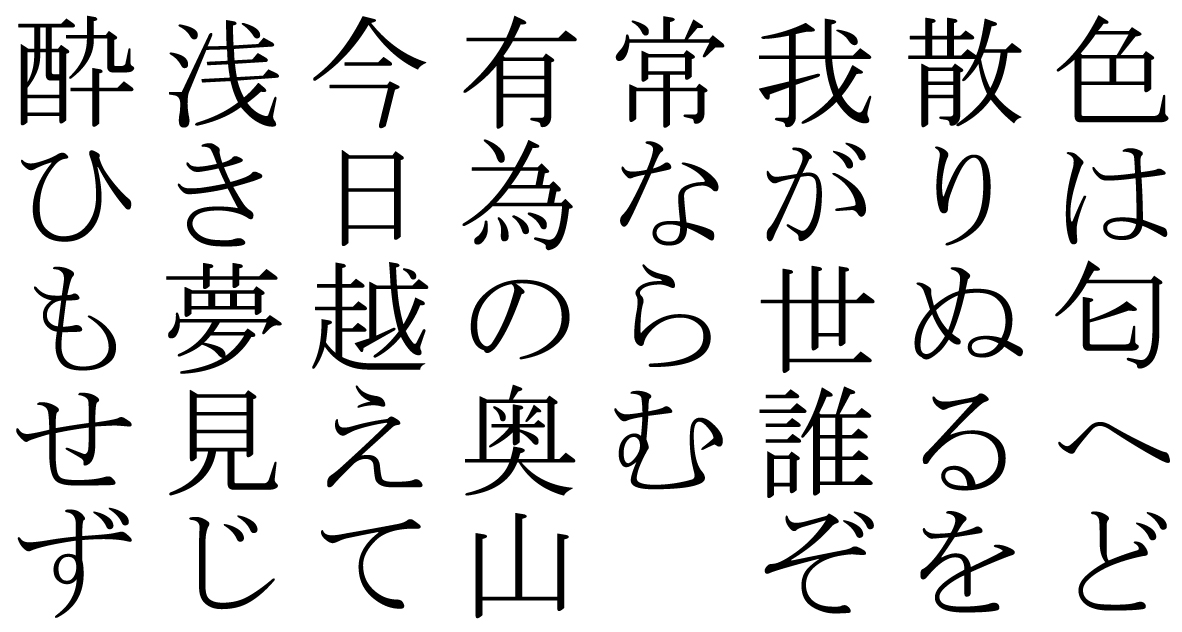
\includegraphics{../data/media/minchou.jpg}}\nopagebreak[4]\par {\smaller \smaller The いろは poem‚ in the 明朝 variant of 楷書 style}\end{center}



\vspace{0.5em}
\begin{center}
\fbox{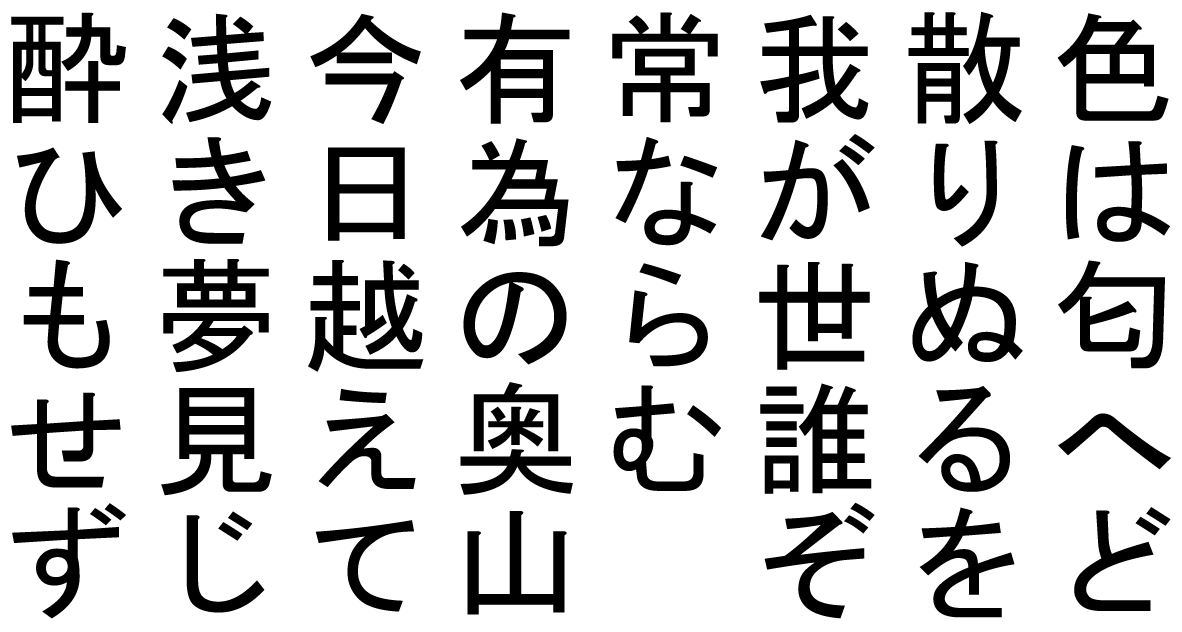
\includegraphics{../data/media/gothic.jpg}}\nopagebreak[4]\par {\smaller \smaller  The いろは poem‚ in the ゴシック  variant of 楷書 style}\end{center}


In addition to the kaisho style‚ there are the two “cursive” styles called \index[english]{Written styles!gyousho}gyousho‚ \index[japanese]{ぎょうしょ (行書)}\ruby{行書}{ぎょうしょ}‚ and \index[english]{Written styles!sousho}sousho‚ \index[japanese]{そうしょ (草書)}\ruby{草書}{そうしょ}‚ which are “simplified” forms of written Japanese. The simplification here refers to the fact that these two styles connect many strokes into single strokes‚ or in extreme cases‚ even simplify entire kanji to single strokes. However‚ this does not make them simpler to read - far from it‚ the simplifications can make it much harder to tell certain kanji apart‚ or look up in a dictionary.

Gyousho is usually associated with handwriting: while we can all write letters the way they come rolling out of a printer‚ we have a special way of writing everything if we do it by hand‚ and in Japanese this is expressed through a slightly more flowing form of kanji and kana‚ connecting strokes but‚ quite often‚ preserving most of the looks of a kanji. Sousho‚ on the other hand‚ is the highly stylised simplifications associated with brush calligraphy — shapes are simplified according to reasonably rigid rules‚ but these simplifications look drastically different from the original shape‚ and certain shapes are simplified in such a way that it is nearly impossible to tell one from another without having received some form of education in reading and writing brush calligraphy. Illustrating this again using the いろは poem:


\vspace{0.5em}
\begin{center}
\fbox{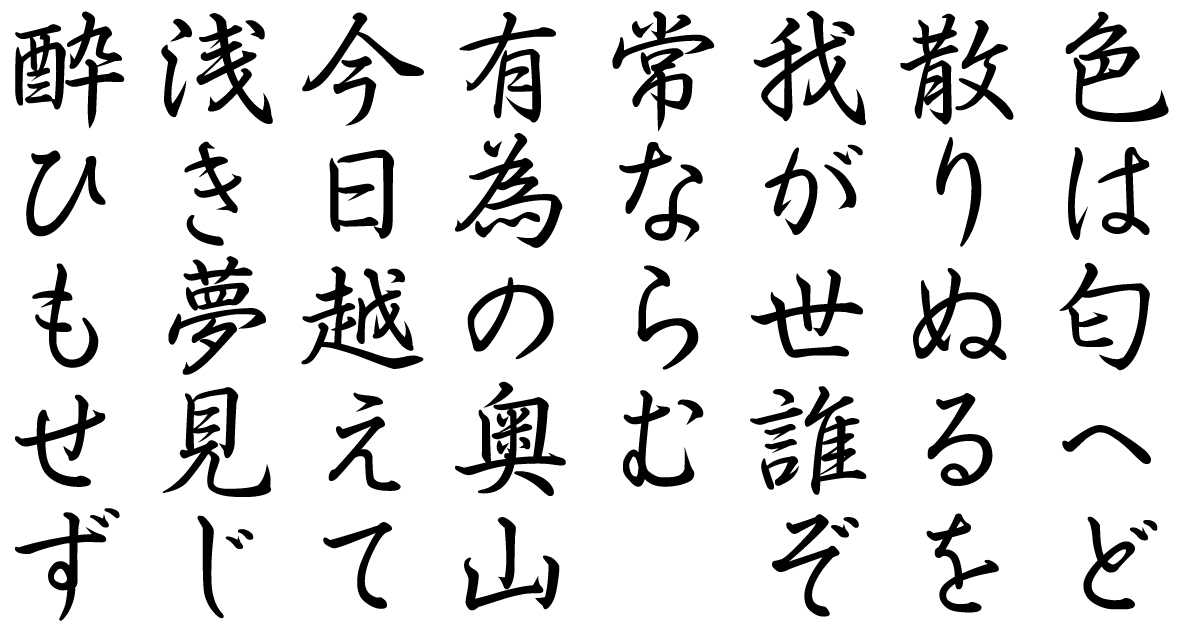
\includegraphics{../data/media/gyousho.jpg}}\nopagebreak[4]\par {\smaller \smaller The いろは poem‚ in 行書 style}\end{center}



\vspace{0.5em}
\begin{center}
\fbox{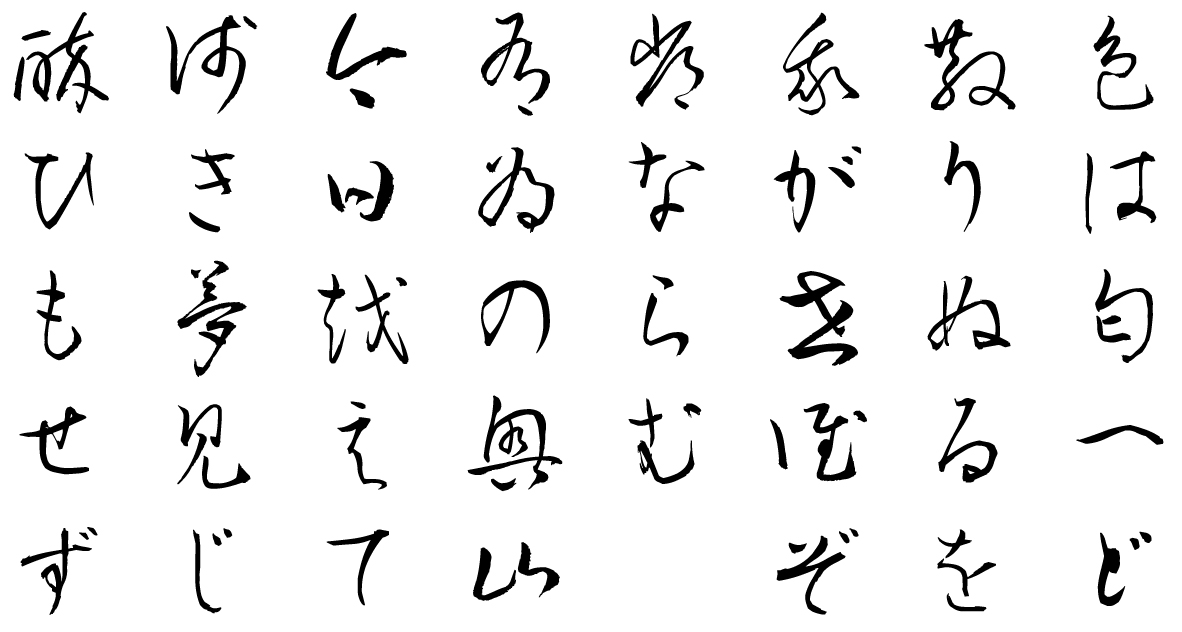
\includegraphics{../data/media/sousho.jpg}}\nopagebreak[4]\par {\smaller \smaller  The いろは poem‚ in 草書 style}\end{center}


Lastly‚ there are two “traditional” styles that you only find used in very specific applications: \index[english]{Written styles!reisho}reisho‚ \index[japanese]{れいしょ (隷書)}\ruby{隷書}{れいしょ}‚ “\index[english]{Square style}square style” or “\index[english]{Block style}block style”‚ and \index[english]{Written styles!tensho}tensho‚ \index[japanese]{てんしょ (篆書)}\ruby{篆書}{てんしょ}‚ “\index[english]{Seal style}seal style”. These two styles are not just traditional but “ancient” styles‚ in that they are styles found used far back in Japanese history on official records and seals (respectively). Reisho is associated with the style of carved kanji on woodblocks (explaining its ‘block style’ name)‚ and is still in use today for things such as traditional signs. Tensho is also still used in modern Japan‚ featuring most prominently in personal stamps — in Japan‚ you do not sign documents with a signature‚ but you put your personal stamp on the document. Everyone who has ever signed something has one of these‚ and you’ll probably know them from the distinctive red-ink kanji-in-a-circle or kanji-in-a-square signs on Chinese and Japanese paintings and brush works. Illustrating these two styles using the いろは again:


\vspace{0.5em}
\begin{center}
\fbox{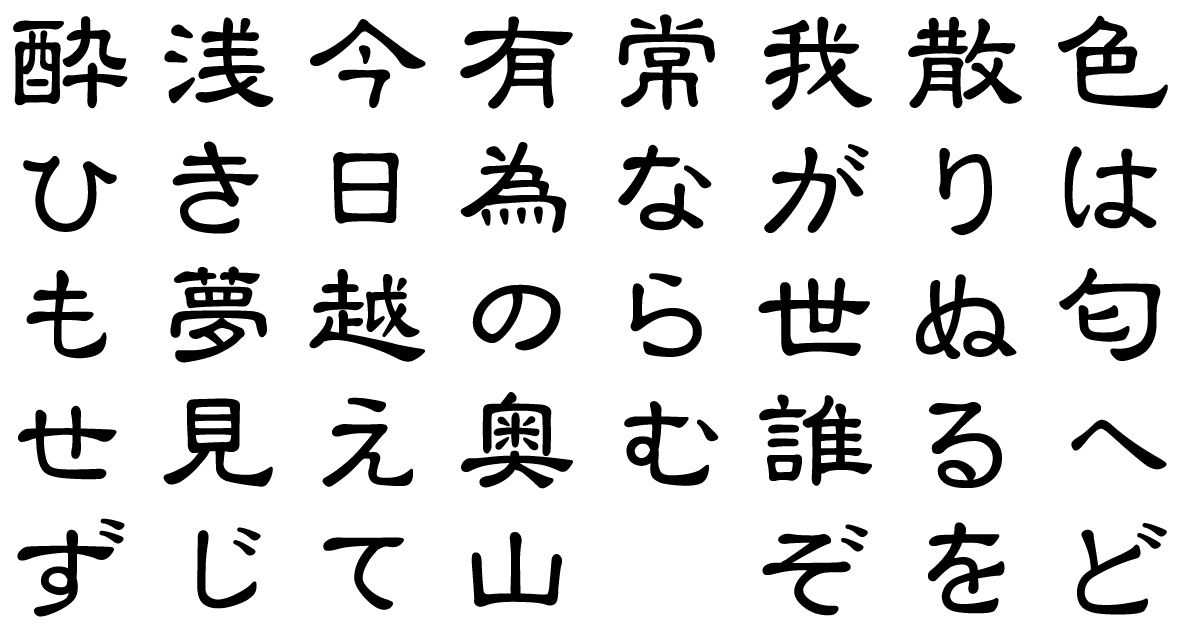
\includegraphics{../data/media/reisho.jpg}}\nopagebreak[4]\par {\smaller \smaller The いろは poem‚ in 隷書 style}\end{center}



\vspace{0.5em}
\begin{center}
\fbox{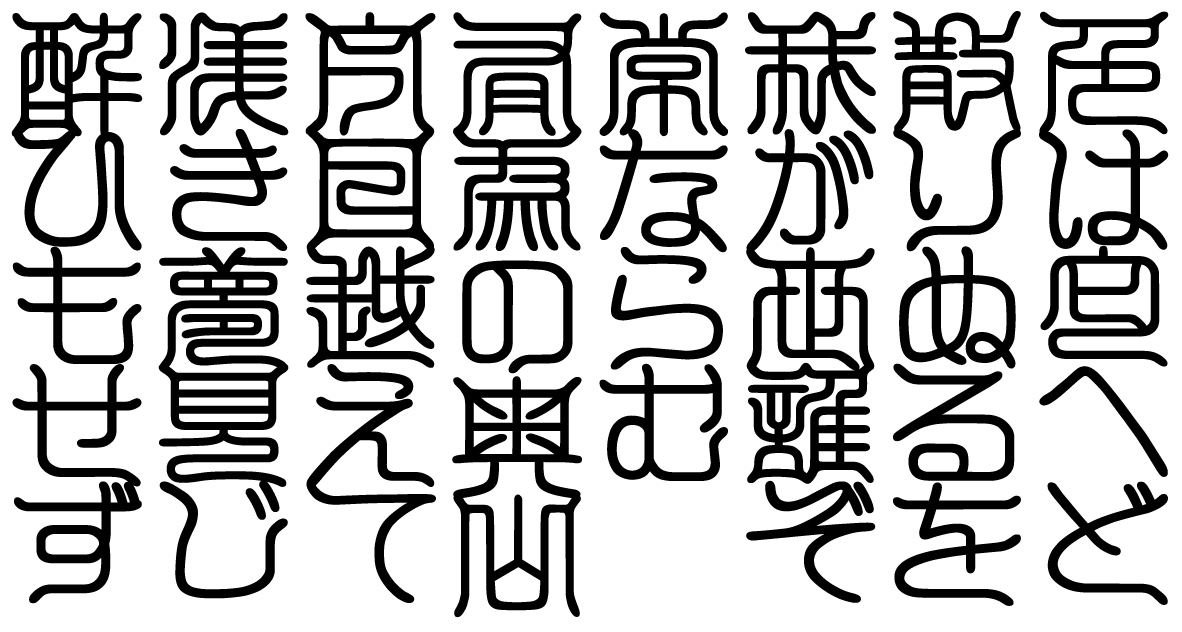
\includegraphics{../data/media/tensho.jpg}}\nopagebreak[4]\par {\smaller \smaller  The いろは poem‚ in 篆書 style}\end{center}


Special dictionaries exist that list kanji in their different forms. These come in the form of \index[english]{Writing dictionary!santaijiten}santaijiten‚ \index[japanese]{さんたいじてん (三体辞典)}\ruby{三体辞典}{さんたいじてん}‚ which list kaisho‚ gyousho and sousho forms (“santai” meaning three forms)‚ and \index[english]{Writing dictionary!gotaijiten}gotaijiten‚ \index[japanese]{ごたいじてん (五体辞典)}\ruby{五体辞典}{ごたいじてん}‚ which list all five forms for a kanji (“gotai” meaning five forms). There are even reference works which don’t so much list the forms in a neatly ordered fashion‚ but show you different interpretation that artists have of the gyousho and sousho forms of kanji‚ which makes them more “artbook” than reference book‚ even when they are invaluable resources to students of Chinese and Japanese calligraphy.

\section{Words and word classes}

With all this talk about lettering‚ one would almost forget that just letters hardly get us anywhere if we don’t know any words to write with them. However‚ Japanese doesn’t have quite the same words as most western languages have. You may have heard the terms “noun” and “verb”‚ and you may even be familiar with terms like “prepositions” and “adverb”‚ but there are quite a number of these word types‚ and we’ll look at all of these in terms of whether or not Japanese uses them‚ and what they look like.

\subsection{\index[english]{Word classes!articles}Articles}

This is a group of words that you rarely think about as real words: in English‚ “the”‚ “a” and “an” are \glslink{article}{articles}\index[english]{Articles}. They precede a word to tell you whether it’s an undetermined ‘something’ (by using “a” or “an”) or a specific ‘something’ (by using “the”). Japanese‚ on the other hand‚ doesn’t have articles at all. It’s not just that it uses a different way to indicate the difference between for instance “a car” and “the car”: there are no simple words you can use to show this difference. This might sound like a rather big stumbling block‚ but there are many languages which do not have articles‚ and the people that use those languages can get the meaning across just fine without them - as we will see when we talk about context later in this chapter.

\subsection{\index[english]{Word classes!verbs}Verbs}

Verbs are words that represent an action either taking place or being performed‚ and can be modified to show things like negatives or past tense. In English‚ words like “fly” and “float” are verbs for actions that are being performed‚ and we can make them negative or past tense: “not fly”‚ “not float”‚ “flew” and “floated” respectively. Similarly‚ words like “walk” and “eat” are verbs for actions that can be performed‚ and we can make them negative or past tense too: “not walk”‚ “not eat”‚ “walked” and “ate” respectively. Verbs also have a regularity: walk and float are regular verbs in that they follow the same rules: past tense is “… + ed”‚ but “fly” and “eat” are \glslink{irregular verb}{irregular}: they do not become “flyed” and “eated”‚ but “flew” and “ate”.

Finally‚ verbs can be \index[english]{Transitive}transitive‚ or \index[english]{Intransitive}intransitive. The verb “walk”‚ for instance‚ is something that you just do. You walk. When you see this kind of construction in a sentence‚ we say that the verb is used “intransitively” - in contrast‚ “eat” is a verb you can either use \glslink{intransitive}{intransitively} (“What are you doing?” - “I’m eating”) or \glslink{transitive}{transitively}: “I eat an apple”. In this use‚ you’re applying the verb’s action to something: “I throw the ball”‚ “I eat an apple”‚ “I fly a plane” are all examples of this. However‚ there is something funny about transitivity: some verbs‚ like “walk”‚ you can only use intransitively (we don’t say that we “walked the street”‚ for instance)‚ but many verbs can be used either intransitively or transitively‚ like “eat”.

There are also a number of verbs that can only be used transitively‚ but these are special verbs‚ typically called \glslink{auxiliary verb}{auxiliary verbs}. In English‚ “have” and “want” are examples of these. Without an additional “something”‚ these verbs do not have any meaning on their own: saying “I have.” or “I want.” is grammatically incorrect. At the very least‚ you’d need to say something like “I have it.” or “I want that.” for the verbs to be used correctly.

Japanese verbs are characterised by a high degree of regularity as‚ except for three verbs‚ all verbs are regular. These regular verbs fall into two categories‚ namely the “five grade” verbs called \index[english]{Verb types!godan}godan‚ \index[japanese]{ごだん (五段)}\ruby{五段}{ごだん}‚ and the “single grade” verbs‚ called \index[english]{Verb types!ichidan}ichidan‚ \index[japanese]{いちだん (一段)}\ruby{一段}{いちだん}. These two categories inflect (take on different \glslink{tense}{tense}‚ \glslink{mood}{mood}‚ etc) in the same way on almost all possible \glslink{inflection}{inflections}‚ but of course differ on some (otherwise there wouldn’t be two categories‚ but just one).

With respect to transitivity‚ Japanese verbs can be a little problematic. Rather than being labelled intransitive or transitive‚ Japanese verbs are labelled as being \index[japanese]{じどうし (自動詞)}\ruby{自動詞}{じどうし} or \index[japanese]{たどうし (他動詞)}\ruby{他動詞}{たどうし}‚ literally “verb that works on its own” and “verb that works paired with something”. Quite often these two verb classifications map to the roles of “intransitive” and “transitive”‚ respectively‚ but sometimes they don’t. For instance‚ traversal verbs (such as ‘walk’‚ ‘run’‚ ‘fly’‚ ‘sail’‚ etc.) are intransitive in English‚ but are 他動詞 in Japanese: they can be used with an object to indicate what is being walked or run over‚ what is being flown through‚ what’s being sailed in‚ etc. As such‚ while in English one does not “fly the sky” or “swim the ocean” (at the very least you’d need a preposition such as “through” or “in” to make those correct English)‚ in Japanese this is exactly what you’re doing.

自動詞 on the other hand do not have a “verb object”; they operate on their own. For instance‚ in English we can say “I understand the text”‚ and if we look at the sentence from a grammatical point of view we can say that ‘the text’ may be considered the verb object for the verb ‘understand’. However‚ in Japan the verb for understanding‚ \ruby{分}{わ}かる‚ is a 自動詞 verb‚ and so even though you’re used to thinking of “understanding” as a transitive verb action‚ you suddenly have to get used to it being an intransitive verb action in Japanese. Particularly at first‚ this can be somewhat confusing‚ but like all foreign languages‚ exposure to frequently used verbs means you’ll quickly develop a sense of how to use them properly (even if you can’t remember the terms ‘intransitive’‚ ‘transitive’‚ 自動詞 and 他動詞!).

\subsection{Nouns}

\glslink{noun}{Nouns} are words that are used to name “somethings”‚ although those somethings don’t need to be things you can actually hold in your hand and look at: “car”‚ “New York”‚ “magnification” and “ambiguity” are all nouns‚ but while you can touch a car‚ or point at New York‚ it’s impossible to point at something and go “that is magnification” or “that is ambiguity”. A good rule of thumb is “if you can say it’s ‘something else’‚ it’s a \index[english]{Word classes!noun}noun”:

\vspace{0.4cm}
\begin{exampleblock}
“This car is old.” \\* 
“New York is hot.” \\* 
“The magnification is high.” \\* 
“This ambiguity is omnipresent.” \\* 
\end{exampleblock}
\vspace{0.2cm}

These are all examples where the noun is said to be something else (and that something else is known as an “adjective”). This even works with things that you might think are verbs‚ but actually aren’t: “walking” for instance looks like it’s a verb‚ because “walk” is a verb‚ but there are instances when “walking” is most definitely a noun. Of the following two sentences‚ the first uses “walking” as a verb‚ while the second uses “walking” as a noun:

\vspace{0.4cm}
\begin{exampleblock}
“I went to work walking.” \\* 
“I like walking.” \\* 
\end{exampleblock}
\vspace{0.2cm}

We can verify that in the first sentence we’re using a verb‚ and in the second a noun‚ by replacing “walking” with a word which we know is a noun‚ like “cheese”:

\vspace{0.4cm}
\begin{exampleblock}
“I went to work cheese.” \\* 
“I like cheese.” \\* 
\end{exampleblock}
\vspace{0.2cm}

The first sentence suddenly makes no sense at all anymore‚ while the second sentence is still perfectly fine. This “words can belong to multiple classes‚ and which it is depends on how it’s used in a sentence” is something quite important to remember when dealing with Japanese‚ as well as learning foreign languages in general.

As a last bit of noun related information‚ in Japanese (as in English‚ in fact) nouns do not inflect. They usually need verbs to indicate negative‚ past tense‚ and other such things: in English we can say “This is not a book” or “This was a book”‚ but the negative and past tense comes from inflections of the verb “be”‚ not the noun itself.

\subsection{\index[english]{Word classes!pronouns}Pronouns}

There is a special class of words called “pronouns” in English‚ which act as if they’re nouns‚ but are used to replace nouns in sentences. The best known pronoun in the English language is the word “\index[english]{Pronouns!it}it”‚ but words like “this”‚ “that” as well as “you” or “we” are all examples of \glslink{pronoun}{pronouns}. Rather than constantly referring directly to what we’re talking about‚ it is far more natural to use pronouns instead:

\vspace{0.4cm}
\begin{exampleblock}
“I bought a really good book. I had already read it‚ having borrowed it from the library last month‚ but I saw it in the book store on discount‚ so I decided to buy it.” \\* 
\end{exampleblock}
\vspace{0.2cm}

In this sentence‚ the pronoun “it” is used quite a number of times‚ replacing “the book” at every instance:

\vspace{0.4cm}
\begin{exampleblock}
“I bought a really good book. I had already read the book‚ having borrowed the book from the library last month‚ but I saw the book in the book store on discount‚ so I decided to buy the book.” \\* 
\end{exampleblock}
\vspace{0.2cm}

This sounds unnatural to English ears‚ even though grammatically speaking there is nothing wrong. In Japanese‚ pronouns are part of a class of words \glslink{colloquial}{colloquially} referred to as “\index[english]{Pronouns!kosoado}kosoado”‚ \index[japanese]{こそあど}こそあど‚ for the fact that they all start with either “ko-”‚ “so-”‚ “a-” or “do-” depending on their level of proximity (for instance‚ ‘this’ vs. ‘that’) and whether they are stative or interrogative (‘that’ vs. ‘what’).

\subsection{Nominalisers}

Japanese has an extra class pertaining to nouns‚ known as the \index[english]{Word classes!nominalisers}nominalisers: words that‚ when used with other words or phrases‚ turn these words or phrases into something that can act as if the whole construction is a noun. In English‚ an example of this is the collection of words “the way in which”:

\vspace{0.4cm}
\begin{exampleblock}
“The way in which the government is handling the issue of criminal law is questionable.” \\* 
\end{exampleblock}
\vspace{0.2cm}

In this sentence‚ “the way in which” is used to turn “the government is handling the issue of criminal law” into a single noun construction. As such we can replace “the way in which the government is handling the issue of criminal law” with a simple pronoun if we wish to talk about it in later sentences:

\vspace{0.4cm}
\begin{exampleblock}
“The way in which the government is handling the issue of criminal law is questionable. It does not seem to be motivated by sound principles‚ but by back-office politics.” \\* 
\end{exampleblock}
\vspace{0.2cm}

Japanese has quite a number of these \glslink{nominaliser}{nominalisers}‚ each with its own meaning and nuance‚ and we shall look at these nominalisers in the chapter on language patterns‚ too.

\subsection{Adjectives}

As we saw in the section on nouns‚ any word that can be used to be “more specific” about a noun is called an adjective. Words like “big”‚ “cold”‚ “square” can all be used as \index[english]{Word classes!adjectives}adjectives to be much more specific about‚ for instance‚ the noun “box”:

\vspace{0.4cm}
\begin{exampleblock}
“This is a box.” \\* 
“This is a square box.” \\* 
“This is a big‚ square box.” \\* 
“This is a big‚ cold‚ square box.” \\* 
\end{exampleblock}
\vspace{0.2cm}

In Japanese‚ there are two types of adjectives‚ namely “\glslink{verbal}{verbal}” adjectives and “nominal” adjectives‚ the difference being that the first type can — unlike in English — be inflected without relying on a \glslink{copula}{copula} verb. In English‚ we have to say “The car was fast”‚ but in Japanese this “was fast” does not use a copula verb such as ‘was’‚ but the adjective itself can convey this meaning. In essence‚ in Japanese we get something akin to “The car is fast-in-past-tense”. The copula stays the way it is‚ but the adjective itself changes‚ something which trips up many beginning students of Japanese.

The \index[english]{Adjective types!na-adjectives}“noun” adjectives behave in the same way English adjectives do‚ needing a copula to change. “It was a square box” is the same in Japanese as it is in English‚ with “is” becoming “was”‚ and the adjective staying the way it is.

While we can use adjectives to be more specific about a noun‚ they cannot be used to be more specific about a verb. As an example‚ in the next two sentences the word “fast” is used as an adjective in the first‚ but is used as a different kind of word in the second sentence:

\vspace{0.4cm}
\begin{exampleblock}
“This is a fast car.” \\* 
“I walked quite fast.” \\* 
\end{exampleblock}
\vspace{0.2cm}

In the first sentence‚ the word “fast” is used to be more specific about the noun “car”‚ but in the second sentence‚ the word “fast” is used to be more specific about the verb action “walk”. While they look like the same word‚ their use falls in different word classes. When used to be specific about a noun‚ a word is called an adjective. When used to be specific about a verb‚ it’s called an \glslink{adverb}{adverb}.

\subsection{\index[english]{Word classes!adverbs}Adverbs}

Using words to be specific about verbs and verb actions is called using them adverbially. In fact‚ in that sentence the word “adverbially” is an adverb‚ letting us be specific about the way in which “using” is used. While in English it can sometimes be confusing as to whether a word is being used as an adjective or as an adverb‚ in Japanese this overlap does not exist: both verbal and nominal adjectives are modified (in different ways) so that they can be used as adverbs instead. Because of this‚ there is no way to mistake whether a word is used as adjective or adverb when you look at a sentence.

In addition to adjectives-turned-adverb‚ Japanese also has words that are only adverbs. The most important of these are the \index[english]{Word classes!quantifiers}quantifiers‚ which include things like “a lot”‚ “not so much” and “often”.

\subsection{\index[english]{Word classes!particles}Particles}

Japanese has an extra word class that isn’t found in most western languages: the \glslink{particles}{particle} class. Words in this class fulfil a wide variety of roles: denoting grammar explicitly‚ adding emphasis‚ disambiguating‚ marking how parts of a sentence bear relation to each other‚ supplying reason‚ contradiction‚ logical arguments‚ you name it — there is probably a particle that can be used for it.

Most particles are \index[english]{Word classes!suffixes}suffixes‚ so that when you use a particle to indicate for instance a contrast between two things‚ it gets added after the first thing‚ rather than adding it in front like in English.

\vspace{0.4cm}
\begin{exampleblock}
English: While (X is the case)‚ (also Y). \\* 
Japanese: (X is the case) while‚ (also Y). \\* 
\end{exampleblock}
\vspace{0.2cm}

Within this word class‚ there is an important subclass known as the \index[english]{Word classes!counters}counters. Like Chinese‚ but very much unlike most western languages‚ counting in Japanese requires not just a knowledge of numbers‚ but also of which particle to use in order to describe the category of things you are counting. In the same way that you can ask for two mugs of beer or two glasses of beer in English‚ you need to use the \glslink{counter}{counter} for “mugs” or “glasses” in Japanese. However‚ while you can ask for “two teas” in an English establishment‚ this kind of request is impossible in Japanese. You have to order “two (units of) tea”‚ where the counter that you chose for your units makes the difference between whether you’re asking for two cups or tea‚ two bags of tea‚ or are accidentally asking for two sheets of tea.

\subsection{\index[english]{Word classes!prefixes}Prefixes}

Some particles‚ as well as some common concept markers‚ are \glslink{prefix}{prefixes} rather than \glslink{suffix}{suffixes} — they are placed in front of words belonging to certain word classes. A handful of special prefixes are used for things like marking words as \index[english]{Honorific}\glslink{honorific}{honorific}‚ performing “inherent” \index[english]{Negation}negation (an English example of which is “the house was windowless” rather than “the house had no windows”)‚ indicating \index[english]{Repetition}repetitions (“rereading a book”) and acting as category marker for categories such as “new”‚ “big” or “most”‚ as well as some more exotic categories such as extents or limits. These will be discussed in detail in the chapter on particles‚ in the section on prefixes.

\subsection{\index[english]{Word classes!onomatopoeia}Onomatopoeia and \index[english]{Word classes!mimesis}mimesis}

Two final word classes which are important to know when dealing with Japanese are the \glslink{onomatopoeia}{onomatopoeia}‚ and the \glslink{mimesis}{mimesis}. Quite a mouthful‚ onomatopoeia (from the Greek onomato-‚ “name”‚ and poi- “to make”) are words that are used to reflect the sounds that things make. For instance‚ “The heavy rock splooshed into the lake” is an example of an onomatopoeic verb. It doesn’t tell us what the rock actually did — namely‚ fall into the water — but implies it by virtue of the sound we know a rock falling in water makes: “sploosh”.

In addition to such \index[english]{“sound” words}“sound” words‚ there are also \index[english]{“state” words}“state” words‚ which do not indicate a particular sound‚ but indicate a particular property. Rare in English‚ an example of this would be the word “gloopy” when describing something. Calling something “gloopy” doesn’t tell you something objective about it‚ but you can surmise it’s probably of a viscous liquid gel-like consistency‚ as well as unpleasant to the touch.

While in English (and in most other western languages) using these words is considered a sign of a poor grasp of the language (after all‚ why use a word like “gloopy” when you can call something a “liquid‚ but viscous‚ unpleasant gel”)‚ and mainly associated with “children’s language”‚ in Japanese using onomatopoeia is essential to natural sounding language: with thousands of these words available to choose from‚ each with its own \glslink{connotation}{connotations} and \glslink{implication}{implications}‚ picking the right onomatopoeia or mimesis at the right time is something that demonstrates a high level of competency in the language.

Onomatopoeia‚ called \index[japanese]{ぎおんご (擬音語)}\ruby{擬音語}{ぎおんご} (‘\index[english]{Giongo}giongo’‚ in which the ‘gi’ part means ‘to mimic’‚ the ‘on’ part means ‘sound’‚ and the ‘go’ part means ‘word’) and mimesis‚ called \index[japanese]{ぎたいご (擬態語)}\ruby{擬態語}{ぎたいご} (‘\index[english]{Gitaigo}gitaigo’‚ in which ‘tai’ means condition or state)‚ are some of the hardest words to learn‚ as they usually carry very specific nuances in meaning. For instance‚ in relation to a leaking tap‚ a Japanese person might say “the water was dripping out”‚ picking one specific word from among a great number of possible onomatopoeia to indicate whether the dripping was intermittent or continuous‚ whether the drips were light or heavy‚ whether their impact in the sink was almost silent or accompanied by backsplash noises‚ each of these qualities being represented by a different onomatopoeic word.

Because of this‚ onomatopoeia and mimesis are an unofficial yardstick when it comes to learning Japanese: if you can use the right onomatopoeic expression at the right time‚ you have mastered a crucial element to speaking natural sounding Japanese.

\subsection{\index[english]{Word classes!compound words}Compound words}

This is technically not a word class‚ but a language feature: in some languages several words can be combined into single words with more meaning that just the individual parts. This practice‚ called compounding‚ is something that some languages have a knack for‚ and some languages simply do not bother with. English‚ for instance‚ is a language in which \glslink{compound}{compound} words are rare — although not unheard of. A common English compound word is the word “teapot”‚ for instance. A combination of the nouns “tea” and “pot”‚ this would have to be a pot for tea. However‚ it’s not really a pot‚ it’s more a decanter. Similarly‚ the “tea” in question is never dry tea leaf‚ even though that’s also called “tea” in English; it has to be boiled water infused with tea leaf. So‚ the single compound noun “teapot” has more meaning than if you looked at the meaning of just the two nouns it was built from.

This “joining up two (or more) words to form new‚ single words” is one of the major dividing lines we can use when trying to classify languages: English is a language sparse in compound words‚ as are French‚ Spanish and Italian‚ but German‚ Danish‚ Dutch‚ Finnish‚ Polish‚ Hungarian‚ Arabic‚ and also Japanese‚ are languages in which compound words are frequently used.

In Japanese‚ nouns are not the only compound words available — compound adjectives as well as compound verbs are also quite common.

\section{\index[english]{Sentence structure}Sentence structure}

In addition to knowing which word classes are used in a language‚ we can also look at languages in terms of how sentences are structured. The most simplistic categorisation of languages in this respect is by looking at the “\glslink{subject}{Subject}‚ \glslink{direct object}{Object} and \glslink{verbs}{Verb}” ordering. This categorisation looks at how languages order these three words classes‚ leading to the conclusions that English‚ for instance‚ is an \index[english]{SVO language}SVO language‚ while Japanese is an \index[english]{SOV language}SOV language: in English‚ most sentences are of the form “we do something”‚ where the subject (“we”) precedes the verb (“do”) which in turn precedes the object (“something”) for that verb. Japanese‚ in contrast‚ follows a different ordering: most sentences are of the form “we‚ something do” (with the comma added purely for ease of reading) where the subject precedes the object for the verb‚ after which the actual verb is used. There are also VSO languages‚ such as formal Arabic or Welsh‚ where the sentence structure is predominantly “do‚ we‚ something” and VOS languages‚ such as Malagasi (used in Madagascar) and Fijian (used in Fiji) where the structure is predominantly “do something‚ we”.

However‚ while this terminology allows us to broadly categorise languages‚ based on what the ‘typically used’ pattern looks like‚ it doesn’t tell us anything about how correct or incorrect sentences are if they do not adhere to these S/V/O “rules”. For instance‚ while “we ate some cake” is a normal English sentence‚ a slightly less conventional but still grammatically perfectly valid English sentence could be “cake; we ate some”. This sentence does not fall in the SVO category that is associated with English‚ but that doesn’t mean it’s an incorrect sentence — it just means the SVO label doesn’t tell the whole story. This becomes particularly apparent when we look at what “minimal sentences” may look like in different languages.

In English‚ a \index[english]{Minimal sentence}minimal sentence (that is‚ one that isn’t considered an expression like “hi!” or “hmm”) consists of a subject and a verb: “I ate” or “she runs” are examples of minimal sentences. Trying to shorten a sentence further — without making the sentence context sensitive — yields broken English‚ which is arguably simply not English. This notion of context is important: if we are asked “How many cookies are left?” and we answer with “four”‚ then this “four” is technically a sentence comprised of a single word‚ and sounds natural. However‚ if we were to use the sentence “four.” on its own‚ it is impossible to tell what we mean by it. This means that while English is an SVO language‚ it’s really an SV(O) language: you need an S‚ you need a V‚ and if you use an O‚ it comes last‚ but you’re not obliged to have one.

When we look at Japanese we see the S/V/O category crumbling even further. Rather than just being an SOV language‚ it’s actually an (S)(O)V language: You need a verb‚ but you don’t need a subject or object at all to form a correct minimal sentence in Japanese. While in English saying “ate” is considered not enough information to make sense of‚ Japanese is a language in which competent listeners or readers fill in these blanks themselves‚ choosing which subject and object make the most sense‚ given what they know about the speaker.  This is what makes Japanese hard: most of the time‚ in every day Japanese‚ subjects and objects will be omitted left and right because‚ as a competent listener‚ you should know what they should have been — Japanese relies heavily on people’s ability to guess what someone else is talking about‚ something which can only come through regular exposure to‚ and use of‚ the language.

\subsection{\index[english]{Word order}Word order}

While it’s all well and good to know that minimal Japanese is an (S)(O)V language‚ it’s also important to know that in Japanese‚ grammar is put directly into the sentence through the use of particles. While in English grammar only becomes apparent through the positioning of words‚ in Japanese words are “tagged”‚ as it were‚ with their grammatical role. To illustrate this‚ an example sentence:

\vspace{0.4cm}
\begin{exampleblock}
\ruby{昨日}{きのう}は\ruby{犬}{いぬ}が\ruby{私}{わたし}のご\ruby{飯}{はん}を\ruby{食}{た}べました。 \\* 
kinou wa inu ga watashi no gohan o tabemashita. \\* 
\end{exampleblock}
\vspace{0.2cm}

This sentence is composed of several “blocks”: 昨日は‚ ‘kinou wa’‚ indicates the noun ‘kinou’ (“yesterday”) as context. In 犬が‚ ‘inu ga’‚ the noun ‘inu’ (“dog”) is marked as verb actor‚ in 私の‚ ‘watashi no’‚ the noun ‘watashi’ (“I”/“me”) is made \glslink{genitive}{genitive} (forming “my”) and linked to ご飯を‚ ‘gohan o’‚ the noun ‘gohan’ (“dinner”) marked as direct verb object‚ with the final word ‘tabemashita’ being the past tense of the verb “eat”:

\vspace{0.4cm}
\begin{exampleblock}
“Yesterday‚ (a/my/our) dog ate my dinner.” \\* 
\end{exampleblock}
\vspace{0.2cm}

In English‚ there is very little position variation possible in this sentence: “A dog ate my dinner‚ yesterday” is still okay‚ but rearranging the sentence to read “Yesterday‚ my dinner ate a dog” completely changes the meaning of the sentence from something unfortunate to something unsettling. In Japanese‚ the explicit presence of grammar markers in a sentence means that rearranging the “blocks” doesn’t change the meaning of the sentence at all:

\vspace{0.4cm}
\begin{exampleblock}
昨日は私のご飯を犬が食べました。 \\* 
kinou wa watashi no gohan o inu ga tabemashita. \\* 
“Yesterday: my dinner‚ (a/my/our) dog ate.” \\* 
\end{exampleblock}
\vspace{0.2cm}

\begin{exampleblock}
私のご飯を、昨日は、犬が食べました。 \\* 
watashi no gohan o‚ kinou wa‚ inu ga tabemashita. \\* 
“My dinner — yesterday — (a/my/our) dog ate.” \\* 
\end{exampleblock}
\vspace{0.2cm}

\begin{exampleblock}
昨日は犬が食べました、私のご飯を。 \\* 
kinou wa inu ga tabemashita‚ watashi no gohan o. \\* 
“Yesterday (a/my/our) dog ate; my dinner.” \\* 
\end{exampleblock}
\vspace{0.2cm}

\begin{exampleblock}
食べました、犬が、私のご飯を、昨日は。 \\* 
tabemashita‚ inu ga‚ watashi no gohan o‚ kinou wa. \\* 
“Ate‚ a dog (did)‚ my dinner‚ yesterday.” \\* 
\end{exampleblock}
\vspace{0.2cm}

All of these are perfectly valid sentences in Japanese‚ because all the words with meaning are explicitly tagged with the role they play in the sentence.  While some of these sentences will sound more usual than others‚ they all mean the same thing. However‚ once we start moving the particles around‚ pairing them with words from different blocks‚ the same problem arises as we saw for English:

\vspace{0.4cm}
\begin{exampleblock}
昨日は(犬が)(私のご飯を)食べました。 \\* 
kinou wa inu ga watashi no gohan o tabemashita \\* 
“Yesterday‚ (a/my/our) dog ate my dinner.” \\* 
\end{exampleblock}
\vspace{0.2cm}

\begin{exampleblock}
昨日は(ご飯が)(私の犬を)食べました。 \\* 
kinou wa gohan ga watashi no inu o tabemashita \\* 
“Yesterday‚ (the) dinner ate my dog.” \\* 
\end{exampleblock}
\vspace{0.2cm}

In summary‚ it is not so much \index[english]{Word order}word order that inherently gives meaning to a sentence in Japanese‚ but the ‘\index[english]{Semantic blocks}semantic blocks’ of words‚ paired with specific particles. Their combination tells you what the block means‚ and what role it plays in a sentence. As long as the pairings are preserved‚ you can order these blocks in any way you like and maintain the same sentence meaning. Which blocks go where‚ finally‚ depends entirely on what you believe is the most important bit of the sentence‚ as is highlighted in the next section.

\subsection{Emphasis}

Another feature of languages is where \index[english]{Emphasis}emphasis lies in a sentence. In English‚ we tend to put the most pressing bit of information early in the sentence‚ and then say whatever is further relevant to this information later in the sentence. The previous sentence is a good example of this: the main point is that “important information comes early”‚ which is found earlier in the sentence than the additional information. In Japanese‚ things are the other way around: the more important the information is‚ the later it will be placed in a sentence.

A rather simple example is the following pair of sentences:

\vspace{0.4cm}
\begin{exampleblock}
“I fell off my bike while riding home today.” \\* 
\end{exampleblock}
\vspace{0.2cm}

\begin{exampleblock}
\ruby{今日}{きょう}は\ruby{自転車}{じてんしゃ}で\ruby{帰}{かえ}り\ruby{中}{ちゅう}で\ruby{転}{ころ}んでしまいました。 \\* 
kyou wa jitensha de kaerichuu de korondeshimaimashita. \\* 
\end{exampleblock}
\vspace{0.2cm}

While the English sentence is up front with the emphasis‚ namely that we fell off our bike‚ the Japanese sentence doesn’t actually tell you what happened until the very last word‚ ‘korondeshimaimashita’ — “(I) (regrettably/unfortunately) fell down”.

Being unfamiliar with this difference in emphasis (point‚ then details in English vs. details‚ then point in Japanese) can lead to confusion when dealing with words in which this ordering is important‚ such as indicating \index[english]{Simultaneous action}simultaneous actions: in English‚ “while”. If someone asks “what are you doing?” and we answer with “eating some dinner while watching TV”‚ then the main activity is eating dinner. The “watching TV” is additional information‚ but not strictly speaking required for the answer to be complete. In Japanese‚ with the same core information and details used‚ the placement is opposite: the Japanese answer “terebi o minagara‚ gohan o tabemasu” lists “watching TV” first (‘terebi o mi-’)‚ then adds the marker for \index[english]{Simultaneous action}simultaneous action (‘nagara’) and then concludes with “eating dinner” (‘gohan o tabemasu’). Both in English and Japanese‚ the concise answer would simply have been “eating dinner”‚ or “gohan o tabemasu”.

Another‚ more common example is the use of “rather”: “I would rather have X than Y” is a well known sentence pattern in English‚ listing the thing with most preference first. This becomes even more obvious in the shortened pattern‚ “I would rather have X”. In Japanese‚ the ‘rather’ construction uses the particle ‘yori’ and‚ like before‚ the order is quite opposite:

\vspace{0.4cm}
\begin{exampleblock}
Y yori X no hou ga ii to omoimasu \\* 
\end{exampleblock}
\vspace{0.2cm}

Trying to project the way ‘rather’ works in English onto what ‘yori’ means can easily lead to confusion: the English word ‘rather’ assumes that the most important bit is on the left‚ so if we think ‘yori’ does the same — because we know it can be translated as ‘rather’ — we might mistakenly believe that this sentence says “I would rather have Y than X”‚ instead of what it really means‚ “I would rather have X than Y”. While potentially confusing at first‚ this reversal of placement for emphasis becomes more intuitive the more one practises Japanese.

However‚ having important information at the end of a sentence leads to a unique problem when interpreting or translating Japanese: how does one deal with trailing sentences? In English‚ when the latter part of a sentence is left off‚ the most important information has already been presented‚ so when the sentence is cut off we might be missing the details‚ but only the details. In Japanese‚ and other languages where more important information comes later in the sentence‚ leaving off the latter part of a sentence leaves a reader or listener with the details‚ but no knowledge of what these details actually apply to!

While‚ of course‚ this doesn’t lead to problems for people who grew up using a language in which emphasis comes later in a sentence‚ this ‘feature’ can be a great pain for people who grew up with “important bits first”. To them‚ it feels very much like the language is based on the concept of “filling in the blanks”‚ without any indication of what can be used to fill them in. Sadly‚ this too can only be remedied through continued exposure to‚ in this case‚ Japanese‚ so that one becomes intuitively familiar with which words might be implied if they’re left off.

\section{\index[english]{Pitch}Pitch and \index[english]{Accent}accents}

Linguistically speaking‚ Japanese - like various other Asian languages such as Thai or Chinese - uses syllable \glslink{pitch}{pitch} to place \glslink{accent}{accents} in words. Quite often you will find this explained as Japanese being a language with two pitch levels‚ high and low‚ which makes it relatively easy to learn compared to a more complicated language (in terms of pitch) such as Chinese‚ which has four pitch levels for \index[english]{Mandarin}Mandarin‚ and at least six for \index[english]{Cantonese}Cantonese. However‚ this creates the false impression that there are only two tones at which you should pronounce Japanese‚ which is simply not true. Instead‚ accent through pitch in Japanese is best described in terms of \index[english]{Tone difference}tone difference:

\begin{enumerate}
\item If a word has its accent on the first syllable‚ then the pitch of the word starts at a high tone and then drops in pitch at the second syllable. After this‚ the pitch may remain either constant‚ or (slowly) go down as the rest of the word is pronounced. Due to this relatively large difference between the first and second syllable‚ the first syllable is considered accented by the Japanese ear.
\item If a word has its accent on a syllable other than the first or the last‚ the pitch may remain constant or rise gradually until the syllable after the one that is accented‚ where the pitch goes down suddenly to create the pitch difference that is considered an accent in Japanese.
\item If a word has its accent on the last syllable‚ the pitch may remain constant or rise gradually until the last syllable‚ which is pronounced at a notably higher pitch‚ marking it as accented to the Japanese ear.
\item If a word has no accent‚ the pitch may remain constant or rise gradually. This covers the majority of Japanese words and while the pitch may change‚ the lack of sudden discontinuous change makes this sound unaccented to the Japanese ear.
\end{enumerate}

The presence and order of pitch change can make the difference between rain (雨) and candy (飴)‚ both pronounced “ame” but with their accents on the first and second syllable respectively‚ or more drastically between an umbrella (傘) and syphilis (瘡)‚ both pronounced “kasa” but again with their accents on the first and second syllable respectively.

For sentences‚ too‚ pitch plays an important role. A sentence ending with a high and then a low syllable‚ compared to the same sentence ending with the last two syllables in neutral pitch‚ will be experienced as a question rather than as a statement‚ for instance. Anger‚ lecturing‚ boredom‚ and a wide variety of emotions can be told from the pitch pattern of a sentence‚ not unlike in most Western languages. However‚ while in western languages pitch only adds emotion‚ in Japanese‚ a misplaced pitch may also change the meaning of the words being used.

\section{\index[english]{Gender roles}Gender roles}

Due to the different \glslink{formality}{formality} levels in Japanese‚ a particular style of speech is often associated with a particular gender — the more polite and \index[english]{Speech patterns!reserved}reserved speech being associated with \index[english]{Speech patterns!female}female speech‚ and the more brash and forward \index[english]{Speech patterns!plain}plain speech being associated with \index[english]{Speech patterns!male}male speech. While this is an understandable association‚ the problem with associating \index[english]{Speech patterns}speech patterns with genders is that people often mistakenly apply backward logic: if the female speech pattern is reserved‚ then reserved speech is female speech.

This isn’t how it works‚ though. Typically‚ speech patterns fall into categories such as polite reserved speech‚ plain \glslink{informal speech}{informal speech} or \index[english]{Speech patterns!honorific}honorific speech‚ which are used by a particular gender more than the other by virtue of statistics. However‚ this does not mean that what is considered “female speech” is never used by men‚ or what is considered “male speech” isn’t used by women‚ as there is no such thing as exclusively male or female speech. A more accurate distinction is to consider speech patterns as \glslink{direct}{direct} versus \glslink{indirect}{indirect} or \glslink{assertive}{assertive} versus \glslink{reserved speech}{reserved}. Women tend to be more reserved and use less direct speech‚ and men tend to be more assertive and use more direct speech. However‚ when the situation warrants it‚ there is nothing to prevent men from using reserved indirect speech‚ or women from using assertive direct speech. It’s all about what the social setting warrants.

This said‚ there are a few words (not speech patterns) that are genuinely \glslink{effeminate}{effeminate} or \index[english]{Speech patterns!masculine}\glslink{masculine}{masculine}‚ such as the \index[english]{Speech patterns!effeminate}effeminate \glslink{dubitative}{dubitative} particle かしら‚ or the masculine personal pronoun \ruby{俺}{おれ}. It is important to notice that the labels used here are “effeminate” and “masculine”‚ and not “female” and “male”. Very effeminate men (such as transvestites or homosexuals) may very well use very effeminate words‚ and hardcore business ball-busting career women may very well use very masculine words to demonstrate their dominance. Again‚ it’s all about the social setting.

\section{Context language}

As mentioned in the section on sentence structure‚ Japanese is a \glslink{context}{context} \index[english]{Context sensitive}sensitive language‚ relying heavily on the reader or listener to be able to keep track of information during a conversation‚ and omitting any information once it has become contextual. Before we look at an example of this‚ we will look at how a “\index[english]{Context}context” differs from a “\index[english]{Subject}subject”‚ as this can cause some confusion: in our day-to-day experience of language‚ the words ‘context’ and ‘subject’ refer to the same thing. If a public speaker at some convention is talking about the physics of Star Trek‚ then we can say that “the subject of his talk is the physics of Star Trek”‚ or that his talk should be interpreted within the context of “the physics of Star Trek”‚ making the two refer to essentially the same idea — a \glslink{topic}{topic}.

Grammatically‚ the terms are much further apart. Rather than both “subject” and “context” being able to refer to some \index[english]{Topic}topic‚ the two mean wildly different things. A “context” is the overall topic of some text or conversation; it doesn’t necessarily have to be mentioned‚ but it is clear what the text or conversation is all about. A “subject”‚ on the other hand‚ refers to specific words in individual sentences within a text or conversation. The best way to indicate the difference when we use the words “context” and “subject” from a grammatical perspective is as follows:

\vspace{0.4cm}
\begin{exampleblock}
“A sentence says something about a subject‚ within a certain context.” \\* 
\end{exampleblock}
\vspace{0.2cm}

For instance‚ given that this section talks about “context”‚ the sentence “It can be a problematic ‘feature’ of Japanese for people who only know English” is readily interpreted as meaning “Context can be a problematic ‘feature’ of Japanese for people who only know English”. You know what “it” refers to because of the context you’re reading it in. Had this sentence been in a section on the sparsity of language‚ then you would have understood “it” to refer to “the sparsity of Japanese”.

In Japanese‚ this concept of “sentences say things about subjects within a certain context” is taken further than in English. The following conversation may illustrate this:

\vspace{0.4cm}
\begin{exampleblock}
A: あたしのコップを\ruby{見}{み}かけませんでしたか？ \\* 
B: ああ、\ruby{見}{み}てません。 \\* 
A: おかしいわ。ついさっきまで\ruby{持}{も}ってたんですけど。 \\* 
B: \ruby{居間}{いま}のテーブルに\ruby{置}{お}いてきてしまったのではないでしょうか。 \\* 
A: あっ……そうかもしれません、ね。 \\* 
\end{exampleblock}
\vspace{0.2cm}

Transcribed‚ this reads:

\vspace{0.4cm}
\begin{exampleblock}
A: atashi no koppu o mikakemasen deshita ka? \\* 
B: aa‚ mitemasen. \\* 
A: okashii wa. tsui sakki made mottetandesukedo. \\* 
B: ima no teeburu ni oitekiteshimatta no dewanai deshou ka. \\* 
A: a… soukamoshiremasen‚ ne. \\* 
\end{exampleblock}
\vspace{0.2cm}

This conversation can be translated to natural sounding English in the following manner:

\vspace{0.4cm}
\begin{exampleblock}
A: “You haven’t seen my cup‚ have you?” \\* 
B: “No‚ I haven’t seen it.” \\* 
A: “That’s odd. I just had it a moment ago.” \\* 
B: “Perhaps you left it on the table in the living room?” \\* 
A: “Ah! That might be.” \\* 
\end{exampleblock}
\vspace{0.2cm}

In this translation there are a number of \index[english]{Contextual simplification}contextual simplifications: “you” has been used to refer to a specific person‚ “it” has been used to contextually refer to the cup in question‚ and “that” has been used by speaker A to refer to what speaker B said. In Japanese‚ rather than using contextual words like this‚ they are simply omitted entirely. If we do a literal translation to English‚ we see a rather different‚ context-heavy kind of conversation:

\vspace{0.4cm}
\begin{exampleblock}
A: “Haven’t seen my cup?” \\* 
B: “Indeed‚ haven’t seen.” \\* 
A: “Odd… had just a moment ago.” \\* 
B: “Could be left on living room table?” \\* 
A: “Ah! Might be so.” \\* 
\end{exampleblock}
\vspace{0.2cm}

It’s not just “it” which has been omitted‚ even personal pronouns are typically left out. This makes for a seemingly very sparse language‚ which can be hard to interpret‚ especially when one is just starting out with the language. For this reason‚ some textbooks and courses will present Japanese sentences with all the contextual information in them — while this does not violate Japanese grammar‚ it does lead to highly artificial sentences‚ existing only in textbooks rather than reflecting the language as it is actually used. Because of this‚ all the examples in this book will try to use “natural” Japanese phrases‚ with contextual words required for the sentence to make sense in translation added in parentheses. For instance:

\vspace{0.4cm}
\begin{exampleblock}
A: okashii wa. tsui sakki made mottetandakedo. \\* 
A: (That’s) odd. (I) just had (it) (a) moment ago. \\* 
\end{exampleblock}
\vspace{0.2cm}

And with that‚ we are finally able to move on from introductory text to the language itself: let’s sink our teeth in some grammar!


\chapter{Verb grammar}

As mentioned in the introductory chapter on syntax‚ there are two classes of verbal words in Japanese: \glslink{verbs}{verbs}‚ and \glslink{verbal adjectives}{verbal adjectives}. Both of these can be considered to consist of two parts: a verbal \glslink{stem}{stem}‚ called the “\index[english]{Gokan}gokan” (\index[japanese]{ごかん (語幹)}\ruby{語幹}{ごかん})‚ which indicates what the core meaning of a verb or verbal adjective is‚ and some additional hiragana called “\index[english]{Okurigana}okurigana” (\index[japanese]{おくりがな (送り仮名)}\ruby{送}{おく}り\ruby{仮名}{がな})‚ which is used to indicate inflection.

Unlike English‚ where verb stems are already usable on their own — the verb stem of “walk” is “walk”‚ for instance — verb stems in Japanese require an inflection indicator in the form of okurigana‚ so before we move on to the actual rules of grammar concerning Japanese verbs and verbal adjectives‚ we must look at how verbs and verbal adjectives are composed in Japanese. We will first be deconstructing the verbs‚ after which we’ll deconstruct the verbal adjectives.

Note that in this chapter‚ as well as all following chapters‚ Japanese will no longer be romanised. So‚ if you haven’t learned the hiragana script yet: now would be a good time to start!

\section{Inflecting}

In English‚ we are used to thinking of verb \index[english]{Inflection}inflections in terms of ‘the verb’ plus some text that indicates the inflection. We consider “walked” to consist of “walk” with “-ed” tacked on the end‚ and “passing” as being “pass” with “-ing” added to it. However‚ many verb forms in English actually use helper verbs‚ so things like “will help”‚ “let’s dance”‚ “be able to dive” are considered verb chains‚ with the helper verb(s) indicating the tense‚ mood and aspect.

In Japanese‚ all verb inflections are in fact chains of helper verbs and verbal adjectives‚ but rather than being a long list of separated verbs like in English‚ they are added to the base verb one by one until all the \index[english]{Inflection!tense}tenses‚ \index[english]{Inflection!mood}moods and \index[english]{Inflection!aspect}aspects have been dealt with. For instance‚ the verb construction \ruby{待}{ま}たされていました means “(I) had been made to wait”. While hard to tell without spaces or a knowledge of verbal grammar at this point‚ this is actually a series of six verbs chained together in a very specific way:

First‚ we see (ま)た‚ the \glslink{imperfect}{imperfect} base form for 待つ‚ “wait”. This base form is used when forming the negative‚ passive‚ causative or ‘pseudo-future’ form of a verb. Then we see され‚ the \glslink{continuative}{continuative} base for the helper verb for causatives‚ される. This base form is a general purpose ‘intermediate form’ for a great number of inflections. Then て‚ the continuative base for the helper verb for conjunction‚ つ. Then い‚ the continuative base for the verb いる‚ “to be” for animate objects. Combined with て it forms the “-ている” form‚ which marks a verb as present progressive. Then まし‚ the continuative base for the helper verb for politeness‚ ます. Then finally た‚ the terminal base for the helper verb for past tense‚ た.

We can see two things in this \glslink{decomposition}{decomposition}. First‚ the ‘core’ verb is all the way at the beginning‚ and the helper verbs follow each other in inflection order: first the causative of “wait” is formed‚ then that is made a present progressive‚ this is then made polite‚ and then finally the whole construction is turned from present to past tense. Second‚ all the verbs are in some “base” form; this is the crucial difference between Japanese verbal grammar and most other languages.

There are five “\index[english]{Inflection!base forms}base forms” which are used in combination with specific inflections‚ and knowing how to identify these base forms makes verbal grammar significantly easier‚ because it lets us view complex verb \glslink{conjugation}{conjugations} in terms of a series of simple “base form” + “helper” rules. For the past tense progressive causative for instance‚ we see a huge inflection that’s really composed of four fairly simple rules‚ applied one after another:

\vspace{0.5cm}
\smaller
\begin{center}
\begin{mytabularcentered}{| l  l  l |}\hline 
\rule{0pt}{2.4ex}inflection & rule & example\\ 
\hline
\rule{0pt}{2.4ex}causative & imperfect base + される & 待つ → 待た + される\\ 
\rule{0pt}{2.4ex}progressive & continuative base + ている & 待たされる → 待たされ + ている\\ 
\rule{0pt}{2.4ex}polite & continuative form + ます & 待たされている → 待たされてい + ます\\ 
\rule{0pt}{2.4ex}past tense & continuative form + た & 待たされています → 待たされていまし + た\\ 
\hline 
\end{mytabularcentered}
\end{center}
\larger
\vspace{0.5cm}


All complex verb constructions can be described in this way‚ being a series of fixed-order simple rules being applied. What’s more‚ because the two different verb classes in Japanese mostly differ in what their base forms look like‚ inflecting verbs in Japanese is mostly a matter of picking the right base form‚ and then applying the same rules for both verb classes‚ making most inflections the same for the two. Verbal adjectives also rely on this concept of “base form” + “helper”‚ and as will become apparent when looking at the rules of grammar for verbal words‚ some inflections are formed by adding verbal adjectives to verbs‚ while others are formed by adding verbs to verbal adjectives.

Without getting ahead of the material‚ let us first examine which base forms are used by verbs and verbal adjectives‚ and what they look like for each of the verbal word classes.

\subsection{\index[english]{Inflection bases}Inflection bases}

Traditionally‚ there are \index[english]{Base forms}six “\glslink{conjugational bases}{base forms}” for Japanese verbal words‚ of which five are still used in modern Japanese. This traditional scheme is called \index[japanese]{ぶんご (文語)}\ruby{文語}{ぶんご}‚ \index[english]{Literary style}literary style‚ and is associated with \index[english]{Classical!Japanese}classical Japanese‚ while the modern scheme is called \index[japanese]{こうご (口語)}\ruby{口語}{こうご}‚ \index[english]{Colloquial style}colloquial style‚ and is associated with normal \index[english]{Modern Japanese}modern Japanese. Because it is always a good idea to look at where a language has come from‚ in order to understand why it does what it does in its current form‚ the relation between classical and modern Japanese will be mentioned wherever possible.

First‚ let’s look at which base forms are used in classical and modern Japanese:

\vspace{0.5cm}
\smaller
\setlength\LTleft\fill
\setlength\LTright\fill
\Needspace{6\baselineskip}
\begin{longtable}[h]{| l  l  l |}\hline
\rule{0pt}{2.4ex}文語 & 口語 & Base for…\\ 
\hline 
\endfirsthead
\hline
\rule{0pt}{2.4ex}文語 & 口語 & Base for…\\ 
\hline 
\endhead
\hline
\endfoot
\hline
\endlastfoot
\rule{0pt}{3.6ex}\index[japanese]{Inflection bases!みぜんけい (未然形)}\rtruby{未然形}{みぜんけい} & 未然形 & \index[english]{Inflection bases!imperfect}Imperfect constructions‚ such as negative form and\\ 
\rule{0pt}{2.4ex} &  & ‘pseudo-future’‚ as well as passive‚ potential‚ honorific\\ 
\rule{0pt}{2.4ex} &  & and causative forms.\\ 
\rule{0pt}{3.6ex}\index[japanese]{Inflection bases!れんようけい (連用形)}\rtruby{連用形}{れんようけい} & 連用形 & \index[english]{Inflection bases!continuative}Continuative and \index[english]{Inflection bases!conjunctive}conjunctive constructions‚ covering the\\ 
\rule{0pt}{2.4ex} &  & majority of constructions involving helper verbs‚ as well\\ 
\rule{0pt}{2.4ex} &  & as joining up sentences and forming nouns.\\ 
\rule{0pt}{3.6ex}\index[japanese]{Inflection bases!しゅうしけい (終止形)}\rtruby{終止形}{しゅうしけい} & no longer used & \index[english]{Inflection bases!finalising}Finalising form. In modern Japanese‚ this role has been\\ 
\rule{0pt}{2.4ex} &  & assumed by the 連体形 instead.\\ 
\rule{0pt}{3.6ex}\index[japanese]{Inflection bases!れんたいけい (連体形)}\rtruby{連体形}{れんたいけい} & 連体形 & \index[english]{Inflection bases!attributive}Attributive constructions (using verbs like adjectives)‚ and\\ 
\rule{0pt}{2.4ex} &  & in modern Japanese‚ finalised form.\\ 
\rule{0pt}{3.6ex}\index[japanese]{Inflection bases!いぜんけい (已然形)}\rtruby{已然形}{いぜんけい} & 已然形 (\index[japanese]{Inflection bases!かていけい (仮定形)}\rtruby{仮定形}{かていけい}) & \index[english]{Inflection bases!perfect}\glslink{perfect}{Perfect} constructions. In modern Japanese this form is only\\ 
\rule{0pt}{2.4ex} &  & used for hypothetical constructions‚ which is why it’s\\ 
\rule{0pt}{2.4ex} &  & colloquially known as the 仮定形‚ “assuming” form.\\ 
\rule{0pt}{3.6ex}\index[japanese]{Inflection bases!めいれいけい (命令形)}\rtruby{命令形}{めいれいけい} & 命令形 & \index[english]{Inflection bases!imperative}Imperative constructions‚ such as commands and\\ 
\rule{0pt}{2.4ex} &  & prohibitive commands.\\ 
\end{longtable}
\larger
\vspace{0.5cm}


The way these bases are formed for the two classes of verbs and the verbal adjectives is the major difference between these verbal classes. Verbs in Japanese are mostly regular (there are only a handful of verbs with irregularities)‚ and fall into one of two classes: “\index[english]{Verb types!godan}godan”‚ \index[japanese]{ごだん (五段)}\ruby{五段}{ごだん}‚ or ‘five grade’ verbs‚ and “\index[english]{Verb types!ichidan}ichidan”‚ \index[japanese]{いちだん (一段)}\ruby{一段}{いちだん}‚ or ‘single grade’ verbs. Both verb classes end‚ in their “dictionary” form‚ on one of the う—row syllables (although not ず‚ and consequently づ‚ and not ふ or ぷ)‚ so that any verb you may encounter can be found in a dictionary to end on う‚ く‚ ぐ‚ す‚ つ‚ ぬ‚ ぶ‚ む or る (the “dictionary” form mentioned here is a common descriptor used in literature on Japanese‚ and is synonymous with the \ruby{連体形}{れんたいけい} form of verbs or verbal adjectives.

The 五段 verbs (also referred to as “\index[english]{Verb types!class i}class I”‚ “\index[english]{Verb types!type i}type I” or “\index[english]{Verb types!u verb}u verb” in literature) can end on any of the aforementioned syllables‚ but 一段 verbs (also referred to as “\index[english]{Verb types!class ii}class II”‚ “\index[english]{Verb types!type ii}type II” or “\index[english]{Verb types!ru verbs}ru verbs” in literature) only end on る. \index[english]{Verbal adjectives}Verbal adjectives — the class of adjectives in Japanese that inflect just like regular verbs do — only come in one class and always end on the syllable い‚ which is why they are also referred to in literature as “\index[english]{Adjective types!i-adjectives}i-adjectives” (a second class of adjectives‚ the adjectival nouns‚ are commonly referred to as “\index[english]{Adjective types!na-adjectives}na-adjectives”). However‚ while it is useful to know on which syllables verbs and verbal adjectives can end‚ bear in mind that just because verbs end on う—row syllables and verbal adjectives end on い‚ not everything ending on an う—row syllable is a verb‚ and not everything ending on い is a verbal adjective — “all cats have four legs‚ but not everything with four legs is a cat”.

Let us look at how the bases for both verbs and the verbal adjectives are formed. Looking at them as a combination of verbal stem and some final syllable(s)‚ the following table describes each of the bases for these word classes:

\vspace{0.5cm}
\smaller
\setlength\LTleft\fill
\setlength\LTright\fill
\Needspace{6\baselineskip}
\begin{longtable}[h]{| l  l  l  l |}\hline
\rule{0pt}{3.6ex}Base & \rtruby{五段}{ごだん} verbs & \rtruby{一段}{いちだん} verbs & verbal adjectives\\ 
\hline 
\endfirsthead
\hline
\rule{0pt}{3.6ex}Base & \rtruby{五段}{ごだん} verbs & \rtruby{一段}{いちだん} verbs & verbal adjectives\\ 
\hline 
\endhead
\hline
\endfoot
\hline
\endlastfoot
\rule{0pt}{3.6ex}stem (\rtruby{語幹}{ごかん}) & remove う—row syllable & remove る & remove い\\ 
\rule{0pt}{2.4ex}未然形 & stem + あ—row syllable & stem & stem + く\\ 
\rule{0pt}{2.4ex}連用形 & stem + い—row syllable & stem & stem + く\\ 
\rule{0pt}{2.4ex}連体形 & stem + う—row syllable & stem + る & stem + い\\ 
\rule{0pt}{2.4ex}已然形 & stem + え—row syllable & stem + れ & stem + けれ\\ 
\rule{0pt}{2.4ex}命令形 & stem + え—row syllable & stem (+ ろ/よ *) & (stem + かれ*)\\ 
\end{longtable}
\larger
\vspace{0.5cm}


In this table‚ the 命令形 for the 一段 verbs and verbal adjectives are starred‚ to indicate there’s something special about them. First‚ the 一段 verb 命令形 is a bit of a problem: the word 命令形 can refer to either the grammatical base form‚ or to the actual verb inflection as it is used in sentences. In classical Japanese‚ both interpretations of the 命令形 were “stem + よ”; the grammatical base form was the same as the final inflected form. However‚ in modern Japanese the final inflected form is either “stem + ろ”‚ if you’re in an area that adheres to \ruby{標準語}{ひょうじゅんご}‚ ‘standard Japanese’ (the kind spoken in Tokyo)‚ or fairly uniformly “stem + よ”‚ if you’re not. This raises the problem that either the 命令形 is listed as two separate forms — something I’m not too fond of — or listing it as just the stem‚ and then telling you the final inflected forms are either 命令形 + ろ or 命令形 + よ depending on where you are. In this book‚ I’ve taken the latter approach.

In addition to this‚ the verbal adjective 命令形 is a point of contention. In \index[english]{Classical!Japanese}classical Japanese‚ verbal adjectives came in two types: く adjectives and し adjectives. Both of these had a regular form‚ as well as a form involving a \glslink{contraction}{contraction} with the verb ある‚ meaning “to be”‚ forming ～かり adjectives. Because of this‚ the し and く versions were ‘pure’ adjectives‚ in that they had no \glslink{imperfect}{imperfective} or \glslink{commanding}{commanding} form; for adjectives those would make no sense. However‚ because of ある‚ the かり variants did have these forms‚ instead missing a finalising and perfect form. This gave rise to the following rather elaborative set of bases in 文語:

\vspace{0.5cm}
\smaller
\setlength\LTleft\parindent
\setlength\LTright\fill
\Needspace{6\baselineskip}
\begin{longtable}[h]{| l  l  l  l  l |}\hline
\rule{0pt}{2.4ex}Base & ～く form & ～かり form & ～し form & ～しかり form\\ 
\hline 
\endfirsthead
\hline
\rule{0pt}{2.4ex}Base & ～く form & ～かり form & ～し form & ～しかり form\\ 
\hline 
\endhead
\hline
\endfoot
\hline
\endlastfoot
\rule{0pt}{2.4ex}未然形 & - & stem + から & - & stem + しから\\ 
\rule{0pt}{2.4ex}連用形 & stem + く & stem + かり & stem+しく & stem + しかり\\ 
\rule{0pt}{2.4ex}終止形 & stem + し & - & stem+し & -\\ 
\rule{0pt}{2.4ex}連体形 & stem + き & stem + かる & stem+しき & stem + しかる\\ 
\rule{0pt}{2.4ex}已然形 & stem + けれ & - & stem + しけれ & -\\ 
\rule{0pt}{2.4ex}命令形 & - & stem + かれ & - & stem + しかれ\\ 
\end{longtable}
\larger
\vspace{0.5cm}


This is a lot of inflectional potential‚ but as classical Japanese transitioned to modern Japanese‚ all these forms have essentially become merged‚ leading to a single inflectional scheme that mixes forms from the ‘pure’ versions of adjectives with the ある-contracted versions of those adjectives‚ leading to the question of which forms are to be considered belonging to the adjective as it exists now‚ and which belong to the verb ある‚ which happens to work together with verbal adjectives a lot. In this book‚ we’ll consider the final inflected 命令形 for verbal adjectives to be a contraction of the verbal adjective’s 連用形 and the 命令形 for the verb ある‚ which is あれ. This gives us “verbal adjective stem + く” + “あれ” → “verbal adjective stem + くあれ”‚ where くあ contracts to か‚ giving us a final rule “stem + かれ”. So‚ in this book‚ verbal adjectives are considered not to have a genuine 命令形 of their own‚ instead relying on the helper verb ある for one. However‚ other books list it as being simply “stem + かれ”‚ and so for completeness it has been included in the earlier table of bases.

Having covered the “what they look like”‚ let’s look at what this means for a number of verbs from both classes‚ and for verbal adjectives:

\vspace{0.5cm}
\smaller
\setlength\LTleft\parindent
\setlength\LTright\fill
\Needspace{6\baselineskip}
\begin{longtable}[h]{| l  l  l  l  l  l |}\hline
\rule{0pt}{2.4ex}五段 verb & 未然形 & 連用形 & 連体形 & 已然形 & 命令形\\ 
\hline 
\endfirsthead
\hline
\rule{0pt}{2.4ex}五段 verb & 未然形 & 連用形 & 連体形 & 已然形 & 命令形\\ 
\hline 
\endhead
\hline
\endfoot
\hline
\endlastfoot
\rule{0pt}{3.6ex}\rtruby{会}{あ}う & 会わ & 会い & 会う & 会え & 会え\\ 
\rule{0pt}{3.6ex}\rtruby{歩}{ある}く & 歩か & 歩き & 歩く & 歩け & 歩け\\ 
\rule{0pt}{3.6ex}\rtruby{急}{いそ}ぐ & 急が & 急ぎ & 急ぐ & 急げ & 急げ\\ 
\rule{0pt}{3.6ex}\rtruby{話}{はな}す & 話さ & 話し & 話す & 話せ & 話せ\\ 
\rule{0pt}{3.6ex}\rtruby{待}{ま}つ & 待た & 待ち & 待つ & 待て & 待て\\ 
\rule{0pt}{3.6ex}\rtruby{死}{し}ぬ & 死な & 死に & 死ぬ & 死ね & 死ね\\ 
\rule{0pt}{3.6ex}\rtruby{学}{まな}ぶ & 学ば & 学び & 学ぶ & 学べ & 学べ\\ 
\rule{0pt}{3.6ex}\rtruby{読}{よ}む & 読ま & 読み & 読む & 読め & 読め\\ 
\rule{0pt}{3.6ex}\rtruby{分}{わ}かる & 分から & 分かり & 分かる & 分かれ & 分かれ\\ 
\rule{0pt}{3.6ex}\rtruby{切}{き}る & 切ら & 切り & 切る & 切れ & 切れ\\ 
\rule{0pt}{3.6ex}\rtruby{売}{う}る & 売ら & 売り & 売る & 売れ & 売れ\\ 
\rule{0pt}{3.6ex}\rtruby{帰}{かえ}る & 帰ら & 帰り & 帰る & 帰れ & 帰れ\\ 
\rule{0pt}{3.6ex}\rtruby{怒}{おこ}る & 怒ら & 怒り & 怒る & 怒れ & 怒れ\\ 
\end{longtable}
\larger
\vspace{0.5cm}


There are two things worth noting in these tables. Firstly‚ the 未然形 for 会う is not a typographical error; it really is わ‚ not あ. This is a left-over from classical Japanese: 五段 verbs ending on う used to be verbs ending on ふ and う (being ‘wu’‚ rather than ‘u’)‚ which inflected respectively as -は‚ -ひ‚ -ふ‚ -へ‚ -へ and -わ‚ -ゐ‚ -う‚ -ゑ‚ -ゑ (\index[japanese]{Obsolete kana!ゐ}ゐ and \index[japanese]{Obsolete kana!ゑ}ゑ being the now obsolete Japanese syllables for ‘wi’ and ‘we’‚ which have not been in use since the written language was reformed in 1946 by cabinet order). However‚ both were pronounced as -わ‚ -い‚ -う‚ -え and -え. When these two verb classes were simplified to today’s 五段 verbs ending on the modern う‚ the 未然形 pronunciation わ was kept‚ as well as its written form.

The second thing worth noting in the table is the seemingly disproportionate number of examples for 五段 verbs ending on -る. The reason for this is that for some verbs ending on る‚ just looking at the verb’s dictionary form is not enough to determine whether it’s actually a 五段 or an 一段 verb‚ so a few examples are needed to show how to tell the two apart. If a verb ends on る‚ and the syllable preceding it in the あ—‚ う— or お—row (such as is the case for 分かる‚ 売る and 起こる) then this is always a 五段 verb. However‚ if the syllable before the る is in the い— or え—row‚ then it might be an 一段 verb instead. The annoying thing is that without actually looking up the verb in a dictionary‚ or seeing it used in some inflected form that lets you spot the difference between a 五段 base and an 一段 base being used‚ there is no way to tell what kind of verb you’re dealing with. Luckily‚ telling the difference when we do have an inflected form is really easy‚ as we can tell from the following 一段 inflection examples (taking note that the 命令形 as used in this book is just the stem):

\vspace{0.5cm}
\smaller
\begin{mytabular}{| l  l  l  l  l  l |}\hline 
\rule{0pt}{2.4ex}一段 & 未然形 & 連用形 & 連体形 & 已然形 & 命令形\\ 
\hline
\rule{0pt}{3.6ex}\rtruby{見}{み}る & 見 & 見 & 見る & 見れ & 見 (ろ/よ)\\ 
\rule{0pt}{3.6ex}\rtruby{伸}{の}びる & 伸び & 伸び & 伸びる & 伸びれ & 伸び (ろ/よ)\\ 
\rule{0pt}{3.6ex}\rtruby{食}{た}べる & 食べ & 食べ & 食べる & 食べれ & 食べ (ろ/よ)\\ 
\hline 
\end{mytabular}
\larger
\vspace{0.5cm}


Comparing this table with the previous one shows that for any inflection involving the 未然形‚ 連用形 or 命令形‚ which cover most verbal inflections‚ we can readily tell the difference between a 五段 and 一段 verb. The only cases that can leave us uncertain are the 連体形 and 已然形 forms. In these cases‚ we’ll just have to resort to checking a dictionary to be sure of which verb class we’re dealing with.

Lastly‚ a list of examples for the verbal adjectives is quite uniform:

\vspace{0.5cm}
\smaller
\begin{mytabular}{| l  l  l  l  l  l |}\hline 
\rule{0pt}{2.4ex}adjective & 未然形 & 連用形 & 連体形 & 已然形 & (命令形)\\ 
\hline
\rule{0pt}{3.6ex}\rtruby{高}{たか}い & 高く & 高く & 高い & 高けれ & (高かれ)\\ 
\rule{0pt}{3.6ex}\rtruby{楽}{たの}しい & 楽しく & 楽しく & 楽しい & 楽しけれ & (楽しかれ)\\ 
\rule{0pt}{3.6ex}\rtruby{薄}{うす}い & 薄く & 薄く & 薄い & 薄けれ & (薄かれ)\\ 
\rule{0pt}{3.6ex}\rtruby{大}{おお}きい & 大きく & 大きく & 大きい & 大きけれ & (大きかれ)\\ 
\hline 
\end{mytabular}
\larger
\vspace{0.5cm}


Of course‚ the examples of verbal adjectives wouldn’t be complete without one very curious verbal adjective:

\vspace{0.5cm}
\smaller
\begin{mytabular}{| l  l  l  l  l  l |}\hline 
\rule{0pt}{2.4ex}adjective & 未然形 & 連用形 & 連体形 & 已然形 & (命令形)\\ 
\hline
\rule{0pt}{3.6ex}\rtruby{執念}{しゅうね}い & 執念く & 執念く & 執念い & 執念けれ & (執念かれ)\\ 
\hline 
\end{mytabular}
\larger
\vspace{0.5cm}


Normally‚ verbal adjectives end on い‚ preceded by either an あ—‚ い—‚ う— or お—row syllable. However‚ 執念い is the only verbal adjective in Japanese that ends in an え—row syllable + い. This is in fact so unusual that it is virtually never used‚ and you will likely not find this adjective in most dictionaries. So‚ because there’s only the one‚ we can safely state that if you find something that ends in い but it has an え—row syllable preceding it‚ it is virtually certain not to be a verbal adjective.

\subsection{\index[english]{Basic inflection}Basic inflections}

Throughout the course of this section we will look at basic inflections for verbs and verbal adjectives‚ as well as look at a small number of particles that are intricately interwoven with verbal grammar. We shall also look at the basic use and formation of nouns and adverbs‚ so that this chapter in effect covers the minimal basics of “\index[english]{Basic Japanese}basic Japanese”. We will start by looking at which particles are essential in order to understand basic verb grammar‚ and will move from there to simple verb forms: present and past tense‚ as well as \glslink{affirmative}{affirmative} and \glslink{negative}{negative} forms. In order to get an overview of the basic concepts involved without offering too much information at once‚ polite verbal grammar will not be introduced until the next chapter‚ after basic grammar has been covered.

\subsubsection{\index[english]{Particles}Particles}

Verbs and verbal adjectives are used in combination with a number of particles to explicitly mark parts of a sentence as relating to them. For verbs‚ these are the particles を‚ に and が‚ and for verbal adjectives this is just the particle が.

First off‚ \index[japanese]{Verb particles!を}を (pronounced as お). This particle is used to mark a transitive verb’s \index[english]{Direct object}direct object. This particle is fairly straightforward and does what one expects from it given this explanation. In “I eat an apple” the noun “apple” is the \glslink{direct object}{direct object} for the verb “eat”‚ and in the corresponding Japanese sentence‚ リンゴを\ruby{食}{た}べる‚ the word リンゴ (‘apple’) is the direct object to the verb 食べる (‘eat’). However‚ not everything that is considered a direct object in Japanese is considered a direct object when translated to English. For instance‚ in Japanese an aeroplane can “fly the air”‚ whereas in English aeroplanes just fly.

Second is \index[japanese]{Verb particles!に}に‚ which broadly speaking marks \index[english]{Verb details}verb details. Translating a sentence using に to English yields the parts marked with に as becoming \index[english]{Indirect object}indirect objects‚ \index[english]{Prepositional phrase}prepositional phrases or even \index[english]{Adverb}adverbs. Anything that is “not the \index[english]{Verb actor}verb actor‚ or the direct object”‚ but adds more details to the verb action‚ will be marked with に. For instance‚ the Japanese sentence メーリに\ruby{花}{はな}を\ruby{買}{か}ってあげた translates to the English sentence “I bought flowers for Mary”‚ with に mapping to the word ‘for’‚ which in English indicates an indirect object. This is hardly its only ‘meaning’; the Japanese sentence ９\ruby{時}{じ}に\ruby{来}{く}る translates to “I’ll be there at nine”‚ with に mapping to the \glslink{preposition}{preposition} ‘at’. Moreover‚ in the Japanese きれいに\ruby{分}{わ}ける‚ translating to the English “to divide cleanly”‚ the に marks the adjective きれい‚ “clean/neat/tidy”‚ as being used adverbially‚ “neatly‚ cleanly”.

Finally‚ the particle \index[japanese]{Verb particles!が}が is an interesting particle. When used with verbal adjectives‚ it marks the thing the adjective applies to. For instance‚ in the English sentence “that car is fast”‚ the adjective “fast” pertains to “that car”. Similarly‚ in the corresponding Japanese sentence その\ruby{車}{くるま}が\ruby{速}{はや}いです‚ the verbal adjective 速い (‘fast’) pertains to その車 (‘that car’). This concept is carried over to verbs‚ too. Some verbs have what would in English be considered a direct object‚ but in Japanese are not considered direct object because the verb does not ‘impart’ its action on it. For instance‚ in “I throw the ball”‚ the throwing action is imparted on the ball. However‚ in “I know the textbook’s material”‚ knowing is not an action imparted ‘on’ the material — in these cases‚ rather than を‚ が is used in Japanese‚ so that for instance “I understand Japanese” is not expressed as \ruby{日本語}{にほんご}を\ruby{分}{わ}かる but as 日本語が分かる. This is particularly obvious when using verbs in passive mode‚ changing for instance “I eat the cake” to “the cake is being eaten by me”. In the corresponding Japanese sentences‚ the particle changes from を to が: ケーキを食べる becomes ケーキが食べられる. In addition to this‚ が may mark a verb’s actor: 車が\ruby{走}{はし}ってる translates to “(The) car is running”. In this role it is effectively doing the same thing as what it does when it is used to link nouns to adjectives.

In addition to these three particles‚ you will also often see the particle \index[japanese]{Verb particles!は}は (pronounced as わ) being used in example sentences. This particle acts as a \index[english]{Disambiguator}disambiguator when a sentence would otherwise be confusing in terms of who or what it was about‚ or what it was in relation to. For instance‚ \ruby{歩}{ある}かない and \ruby{今日}{きょう}は歩かない translate to “I do not walk” and “I won’t be walking today” by virtue of the second sentence disambiguating the context from as broad as possible (i.e.‚ ‘in general’)‚ to ‘just today’ (今日). This can have some perhaps unexpected side effects‚ too: when saying \ruby{私}{わたし}は\ruby{泳}{およ}ぎません‚ “I do not swim”‚ the explicit presence of 私は means that you apparently felt that you needed to \index[english]{Disambiguate}disambiguate the statement‚ which means any listener will suddenly wonder who then ‘does swim’‚ as opposed to you. On the other hand‚ 私が泳ぎません merely means “I do not swim”‚ using が to mark yourself as verb actor for \ruby{泳}{およ}ぐ.

\subsubsection{Verbal grammar - \index[english]{Inflections!present tense}present tense}

Before we look at how to form the \glslink{present tense}{present tense}‚ a note. There is no distinction between present tense such as “I walk” and indicative \index[english]{Inflections!future tense}future tense such as “I will walk”. Both roles are performed by the same verb form in Japanese: the \index[japanese]{れんたいけい (連体形)}\ruby{連体形}{れんたいけい}. Any verb or verbal adjective in 連体形 is automatically in present/indicative \glslink{future tense}{future tense}. Listing this form for example words from all three verbal classes‚ we see the following:

\vspace{0.5cm}
\smaller
\begin{mytabular}{| l  l  l  l |}\hline 
\rule{0pt}{2.4ex} & 連体形 & meaning & plain present affirmative\\ 
\hline
\rule{0pt}{3.6ex}五段 verb & \rtruby{歩}{ある}く & walk & 連体形: 歩く\\ 
\rule{0pt}{3.6ex}一段 verb & \rtruby{見}{み}る & see & 連体形: 見る\\ 
\rule{0pt}{3.6ex}verbal adjective & \rtruby{高}{たか}い & high‚ expensive & 連体形: 高い\\ 
\hline 
\end{mytabular}
\larger
\vspace{0.5cm}


Some examples of the present tense used in simple sentences:

\vspace{0.4cm}
\begin{exampleblock}
\ruby{今日}{きょう}は歩く。 \\* 
Today (I’ll) walk. \\* 
\end{exampleblock}
\vspace{0.2cm}

\begin{exampleblock}
テレビを見る。 \\* 
(I) watch TV. \\* 
\end{exampleblock}
\vspace{0.2cm}

\begin{exampleblock}
これが高い。 \\* 
This is expensive. \\* 
\end{exampleblock}
\subsubsection{\index[english]{Inflections!negative}Negative}


Having covered the present affirmative tense‚ the next important basic inflection is the negative form. In Japanese‚ negative verb and verbal adjective forms are created with the \index[english]{Helper adjective of negation}helper adjective of negation‚ \index[japanese]{ない}ない (無い)‚ or using the rather classical verb ぬ which will be discussed after polite forms have been introduced later in this chapter.

ない is actually a verbal adjective‚ and so inflects like any other verbal adjective:

\vspace{0.5cm}
\smaller
\begin{mytabular}{| l  l |}\hline 
\rule{0pt}{2.4ex}bases & form\\ 
\hline
\rule{0pt}{2.4ex}未然形 & なく\\ 
\rule{0pt}{2.4ex}連用形 & なく\\ 
\rule{0pt}{2.4ex}連体形 & ない\\ 
\rule{0pt}{2.4ex}已然形 & なけれ\\ 
\hline 
\end{mytabular}
\larger
\vspace{0.5cm}


This helper is combined with both verbs and verbal adjectives by joining up with the 未然形‚ or imperfect base:

\vspace{0.5cm}
\smaller
\begin{mytabular}{| l  l  l  l |}\hline 
\rule{0pt}{2.4ex} & 連体形 & meaning & plain present negative\\ 
\hline
\rule{0pt}{3.6ex}五段 verb & \rtruby{歩}{ある}く & walk & 未然形+ない: 歩かない\\ 
\rule{0pt}{3.6ex}一段 verb & \rtruby{見}{み}る & see & 未然形+ない: 見ない\\ 
\rule{0pt}{3.6ex}verbal adjective & \rtruby{高}{たか}い & high‚ expensive & 未然形+ない: 高くない\\ 
\hline 
\end{mytabular}
\larger
\vspace{0.5cm}


Recycling our example sentences from the present tense section‚ we get the following sentences:

\vspace{0.4cm}
\begin{exampleblock}
\ruby{今日}{きょう}は歩かない。 \\* 
Today (I) don’t/won’t walk. \\* 
\end{exampleblock}
\vspace{0.2cm}

\begin{exampleblock}
テレビを見ない。 \\* 
(I) don’t/won’t watch TV. \\* 
\end{exampleblock}
\vspace{0.2cm}

\begin{exampleblock}
これが高くない。 \\* 
This isn’t expensive. \\* 
\end{exampleblock}
\vspace{0.2cm}

However‚ please note that this rule does not apply to the special verb ある‚ which we shall treat in the next section. Rather than becoming あらない‚ it is simply replaced with ない.

(On a final note‚ it is imperative this ない should never be confused with another adjective pronounced ない‚ 亡い‚ as that means “deceased”)

\subsection{Basic inflections for \index[english]{Irregular verbs}irregular verbs and verbal adjectives}

There are three irregular verbs in Japanese that we need to look at before moving on to further inflections‚ being \index[japanese]{する}する‚ “do”/“decide on”‚ \index[japanese]{くる (来る)}\ruby{来}{く}る‚ “come” and \index[japanese]{ある}ある‚ “exist” (for \glslink{inanimate}{inanimate} things).

\subsubsection{The irregular verb する}

Looking at \index[japanese]{する}する‚ ‘do’‚ first‚ we see the following bases and inflection table:

\vspace{0.5cm}
\smaller
\begin{mytabular}{| l  l |}\hline 
\rule{0pt}{2.4ex}base & form\\ 
\hline
\rule{0pt}{2.4ex}未然形 & さ‚ せ‚ し\\ 
\rule{0pt}{2.4ex}連用形 & し\\ 
\rule{0pt}{2.4ex}連体形 & する\\ 
\rule{0pt}{2.4ex}已然形 & すれ\\ 
\rule{0pt}{2.4ex}命令形 & せ(よ)‚ し(ろ)‚ せい\\ 
\hline 
\end{mytabular}
\larger
\vspace{0.5cm}

\smaller
\begin{mytabular}{| l  l  l |}\hline 
\rule{0pt}{2.4ex} & affirmative & negative\\ 
\hline
\rule{0pt}{2.4ex}plain & 連体形 & “し”—未然形+ない: しない\\ 
\hline 
\end{mytabular}
\larger
\vspace{0.5cm}


We see that する actually has three different 未然形 forms‚ as well as three different 命令形 forms — which of these gets used is fully determined by which inflection you’re going for‚ making this verb a bit trickier than any of the other verbs in the language. Luckily‚ it’s such a common verb that even though it’s highly irregular you will most likely become familiar with all its inflections fairly quickly by virtue of them popping up almost as often as all other verbs put together.

Technically‚ する is considered a サ—\ruby{変}{へん} verb‚ or “irregular verb‚ operating on the サ column”. For the most part‚ it inflects as an 一段 verb‚ but there are rules for what pronunciation to use when using which base‚ which makes it a truly irregular verb.

する has two common “variations”: \index[japanese]{ずる}ずる and \index[japanese]{じる}じる. Both of these are typically found used as a verb in a noun/verb compound (meaning they are paired with a noun without using any particles)‚ and only constitute a small number of all verbs in Japanese. However‚ while only used in a small number of verbs‚ some of those verbs are quite common and frequently used‚ so knowing how to inflect these two verbs is not unimportant.

\vspace{0.5cm}
\smaller
\begin{mytabular}{| l  l  l  l |}\hline 
\rule{0pt}{2.4ex}base & する & ずる & じる\\ 
\hline
\rule{0pt}{2.4ex}未然形 & さ‚ せ‚ し & ざ‚ ぜ‚ じ & じ\\ 
\rule{0pt}{2.4ex}連用形 & し & じ & じ\\ 
\rule{0pt}{2.4ex}連体形 & する & ずる & じる\\ 
\rule{0pt}{2.4ex}已然形 & すれ & ずれ & じれ\\ 
\rule{0pt}{2.4ex}命令形 & せ(よ)‚ し(ろ)‚ せい & ぜ(よ)‚ じ(ろ)‚ ぜい & じ(よ‚ ろ)\\ 
\hline 
\end{mytabular}
\larger
\vspace{0.5cm}

\smaller
\begin{mytabular}{| l  l  l |}\hline 
\rule{0pt}{2.4ex} & affirmative & negative\\ 
\hline
\rule{0pt}{2.4ex}する & 連体形 & “し”—未然形+ない: しない\\ 
\rule{0pt}{2.4ex}ずる & 連体形 & “じ”—未然形+ない: じない\\ 
\rule{0pt}{2.4ex}じる & 連体形 & “じ”—未然形+ない: じない\\ 
\hline 
\end{mytabular}
\larger
\vspace{0.5cm}


For ずる‚ the “ざ” and “ぜ” 未然形 are actually not used a lot in modern Japanese anymore. Instead‚ you will find じ used for virtually all 未然形 constructions‚ with ざ and ぜ indicating respectively classical and non-classical older style Japanese‚ instead.

\subsubsection{The irregular verb \ruby{来}{く}る}

\index[japanese]{くる (来る)}\ruby{来}{く}る (‘come’) on the other hand‚ inflects like any normal 一段 verb (except for a slightly different 命令形)‚ but shares する’s irregularity: the pronunciation for its stem changes for each base. However‚ unlike for する there is only one pronunciation for each base‚ so inflection doesn’t involve “picking the right pronunciation”‚ but merely remembering it:

\vspace{0.5cm}
\smaller
\begin{mytabular}{| l  l  l |}\hline 
\rule{0pt}{2.4ex}base & kanji form & pronunciation\\ 
\hline
\rule{0pt}{2.4ex}未然形 & 来 & こ\\ 
\rule{0pt}{2.4ex}連用形 & 来 & き\\ 
\rule{0pt}{2.4ex}連体形 & 来る & くる\\ 
\rule{0pt}{2.4ex}已然形 & 来れ & くれ\\ 
\rule{0pt}{2.4ex}命令形 & 来い & こい\\ 
\hline 
\end{mytabular}
\larger
\vspace{0.5cm}

\smaller
\begin{mytabular}{| l  l  l |}\hline 
\rule{0pt}{2.4ex} & affirmative & negative\\ 
\hline
\rule{0pt}{2.4ex}plain & 連体形 & 未然形+ない: こない\\ 
\hline 
\end{mytabular}
\larger
\vspace{0.5cm}


As is evident from the table of bases‚ and the table of inflections‚ this verb is virtually indistinguishable from any other 一段 verb. However‚ in spoken language its irregularity is plainly obvious.

\subsubsection{The irregular verb ある}

Finally‚ the verb \index[japanese]{ある}ある‚ “exist” (for inanimate things) has seemingly normal bases‚ but its inflection is quite special:

\vspace{0.5cm}
\smaller
\begin{mytabular}{| l  l |}\hline 
\rule{0pt}{2.4ex}base & form\\ 
\hline
\rule{0pt}{2.4ex}未然形 & あら\\ 
\rule{0pt}{2.4ex}連用形 & あり\\ 
\rule{0pt}{2.4ex}連体形 & ある\\ 
\rule{0pt}{2.4ex}已然形 & あれ\\ 
\rule{0pt}{2.4ex}命令形 & あれ\\ 
\hline 
\end{mytabular}
\larger
\vspace{0.5cm}

\smaller
\begin{mytabular}{| l  l  l |}\hline 
\rule{0pt}{2.4ex} & affirmative & negative\\ 
\hline
\rule{0pt}{2.4ex}plain & 連体形 & \index[japanese]{ない}ない\\ 
\hline 
\end{mytabular}
\larger
\vspace{0.5cm}


This verb is irregular in all its negative forms: rather than using the 未然形+ない rule‚ just ない itself is used. Thus‚ we see the following:

\vspace{0.4cm}
\begin{exampleblock}
\ruby{本}{ほん}がある。 \\* 
“There is a book.” \\* 
\end{exampleblock}
\vspace{0.2cm}

\begin{exampleblock}
本がない。 \\* 
“There is no book.” \\* 
\end{exampleblock}
\subsubsection{The irregular adjective いい}


In addition to these verbs‚ there is the irregular verbal adjective \index[japanese]{いい}いい‚ “good”‚ which is actually the irregular verbal adjective \index[japanese]{よい}よい:

\vspace{0.5cm}
\smaller
\begin{mytabular}{| l  l |}\hline 
\rule{0pt}{2.4ex}base & form\\ 
\hline
\rule{0pt}{2.4ex}未然形 & \index[japanese]{よく}よく\\ 
\rule{0pt}{2.4ex}連用形 & よく\\ 
\rule{0pt}{2.4ex}連体形 & よい‚ いい\\ 
\rule{0pt}{2.4ex}已然形 & よけれ\\ 
\hline 
\end{mytabular}
\larger
\vspace{0.5cm}

\smaller
\begin{mytabular}{| l  l  l |}\hline 
\rule{0pt}{2.4ex} & affirmative & negative\\ 
\hline
\rule{0pt}{2.4ex}plain & いい & 未然形+ない: よくない\\ 
\hline 
\end{mytabular}
\larger
\vspace{0.5cm}


The only irregularity for this verbal adjective is its 連体形‚ which is technically よい‚ but is almost always used as いい instead. Of the two‚ いい is actually considered the plain pronunciation‚ and よい a formal variant. Not knowing that these two are actually the same adjective can lead to confusion in more complex inflections‚ such as when the adjective いい turns into the past tense \index[japanese]{よかった}よかった.

\subsubsection{\index[english]{Inflections!past tense}Past tense}

The last basic inflection we will look at on its own in this chapter is the \glslink{past tense}{past tense}‚ which relies on the classical helper verb for past tense‚ \index[japanese]{た}た. This helper verb has the following bases:

\vspace{0.5cm}
\smaller
\begin{mytabular}{| l  l |}\hline 
\rule{0pt}{2.4ex}base & form\\ 
\hline
\rule{0pt}{2.4ex}未然形 & たろ\\ 
\rule{0pt}{2.4ex}連体形 & た\\ 
\rule{0pt}{2.4ex}已然形 & \index[japanese]{たら}たら\\ 
\hline 
\end{mytabular}
\larger
\vspace{0.5cm}


This verb has no 連用形 (it doesn’t make sense to mark something as a past tense and then continue inflecting it to something else)‚ nor does it have a 命令形 (because one cannot command someone to do something in the past). It is combined with verbal 連用形 forms‚ being wholly unremarkable for the 一段 verbs‚ simply pairing up with the 連用形‚ but being not quite so unremarkable for 五段 verbs. While in classical Japanese‚ the same rule applies as for 一段 verbs‚ in modern Japanese most past tenses for 五段 verbs have become contracted‚ as we can see in the following table:

\vspace{0.5cm}
\smaller
\setlength\LTleft\fill
\setlength\LTright\fill
\Needspace{6\baselineskip}
\begin{longtable}[h]{| l  l  l  l  l |}\hline
\rule{0pt}{2.4ex}五段 & 連用形 & \index[english]{Inflections!classical past tense}classical past tense & \index[english]{Inflections!modern past tense}modern past tense & change ‘rule’\\ 
\hline 
\endfirsthead
\hline
\rule{0pt}{2.4ex}五段 & 連用形 & \index[english]{Inflections!classical past tense}classical past tense & \index[english]{Inflections!modern past tense}modern past tense & change ‘rule’\\ 
\hline 
\endhead
\hline
\endfoot
\hline
\endlastfoot
\rule{0pt}{3.6ex}\rtruby{話}{はな}す & 話し & 連用形+た: 話した & 話した & す verbs: no change\\ 
\rule{0pt}{3.6ex}\rtruby{歩}{ある}く & 歩き & 連用形+た: 歩きた & 歩いた & く verbs: きた → いた\\ 
\rule{0pt}{3.6ex}\rtruby{急}{いそ}ぐ & 急ぎ & 連用形+た: 急ぎた & 急いだ & ぐ verbs: ぎた → いだ\\ 
\rule{0pt}{3.6ex}\rtruby{死}{し}ぬ & 死に & 連用形+た: 死にた & 死んだ & ぬ verbs: にた → んだ\\ 
\rule{0pt}{3.6ex}\rtruby{学}{まな}ぶ & 学び & 連用形+た: 学びた & 学んだ & ぶ verbs: びた → んだ\\ 
\rule{0pt}{3.6ex}\rtruby{読}{よ}む & 読み & 連用形+た: 読みた & 読んだ & む verbs: みた → んだ\\ 
\rule{0pt}{3.6ex}\rtruby{会}{あ}う & 会い & 連用形+た: 会いた & 会った & う verbs: いた → った\\ 
\rule{0pt}{3.6ex}\rtruby{待}{ま}つ & 待ち & 連用形+た: 待ちた & 待った & つ verbs: ちた → った\\ 
\rule{0pt}{3.6ex}\rtruby{分}{わ}かる & 分かり & 連用形+た: 分かりた & 分かった & る verbs: りた → った\\ 
\rule{0pt}{2.4ex}ある & あり & 連用形+た: ありた & あった & る verbs: りた → った\\ 
\end{longtable}
\larger
\vspace{0.5cm}


These rules for contraction in 五段 verbs (luckily) do not just apply to the past tense‚ but to several other inflections (namely the continuative \index[japanese]{て form}て form‚ which is tremendously important to know‚ the representative \index[japanese]{たり}たり form‚ and the \glslink{conditional}{conditional} \index[japanese]{たら}たら form)‚ so that this is not a set of rules you will need to remember for a single inflection‚ but applies to a number of often used inflections‚ making the exception itself somewhat ‘regular’.

Of course‚ there are a few exceptions to these rules. First up‚ 行く‚ which follows the “wrong” rule:

\vspace{0.5cm}
\smaller
\begin{center}
\begin{mytabularcentered}{| l  l  l  l |}\hline 
\rule{0pt}{2.4ex}verb & 連用形 & classical past tense & modern past tense\\ 
\hline
\rule{0pt}{3.6ex}\index[japanese]{いく (行く)}\rtruby{行}{い}く & 行き & 連用形+た & \index[japanese]{いった}いった\\ 
\hline 
\end{mytabularcentered}
\end{center}
\larger
\vspace{0.5cm}


The verb 行く‚ pronounced いく or \index[japanese]{ゆく (行く)}ゆく (the first being used in every day life‚ the latter being used in poetry and song lyrics)‚ does not follow the contraction rule for 五段 verbs ending on く. There is no real reason for this‚ other than “that’s just how people use it”. In all other respects‚ 行く is just another 五段 verb. Luckily‚ this is not some obscure verb you will run into only occasionally and will have forgotten this exception for: 行く means “go”‚ and is used so frequently you will not get a chance to forget it has an irregular past tense.

Secondly‚ there is a (very small) set of verbs that have a rather abnormal past tense‚ based on adding た to the 連体形 instead of the 連用形. These verbs are mostly used in writing‚ and in formal speech‚ but since there are only two (with two kanji forms each) it cannot hurt to look at them:

\vspace{0.5cm}
\smaller
\begin{mytabular}{| l  l  l |}\hline 
\rule{0pt}{2.4ex}verb & meaning & past tense\\ 
\hline
\rule{0pt}{3.6ex}\rtruby{問}{と}う & ask‚ question‚ accuse & 問うた\\ 
\rule{0pt}{3.6ex}\rtruby{訪}{と}う & 〃 & 訪うた\\ 
\rule{0pt}{3.6ex}\rtruby{乞}{こ}う & ask & 乞うた\\ 
\rule{0pt}{3.6ex}\rtruby{請}{こ}う & 〃 & 請うた\\ 
\hline 
\end{mytabular}
\larger
\vspace{0.5cm}


These verbs can‚ technically‚ also be inflected like regular 五段 verbs‚ but since they are mostly reserved for formal spoken and literary written Japanese‚ if you encounter them you will most likely encounter them as 連体形 + た.

For 一段 verbs things are a lot simpler‚ and we see a regular table of inflection:

\vspace{0.5cm}
\smaller
\begin{mytabular}{| l  l  l |}\hline 
\rule{0pt}{2.4ex}一段 & 連用形 & past tense\\ 
\hline
\rule{0pt}{3.6ex}\rtruby{見}{み}る & 見 & 連用形+た: 見た\\ 
\rule{0pt}{3.6ex}\rtruby{伸}{の}びる & 伸び & 連用形+た: 伸びた\\ 
\rule{0pt}{3.6ex}\rtruby{食}{た}べる & 食べ & 連用形+た: 食べた\\ 
\hline 
\end{mytabular}
\larger
\vspace{0.5cm}


And for the irregular verbs we see the same‚ bearing in mind that the stems have a different pronunciation:

\vspace{0.5cm}
\smaller
\begin{mytabular}{| l  l  l |}\hline 
\rule{0pt}{2.4ex}irregular verb & 連用形 & past tense\\ 
\hline
\rule{0pt}{2.4ex}する & し & 連用形+た: した\\ 
\rule{0pt}{3.6ex}\rtruby{来}{く}る & き & 連用形+た: きた\\ 
\hline 
\end{mytabular}
\larger
\vspace{0.5cm}


To form the plain past negative‚ rather than just the plain past‚ we have to take the plain present negative based on \index[japanese]{ない}ない‚ and turn this into a past tense‚ which means we need to look at how to form the past tense for verbal adjectives in general first.

For verbal adjectives‚ rather than a plain inflection‚ the adjectives work together with the verb \index[japanese]{ある}ある (“to be”‚ for inanimate objects and concepts). However‚ because ある is a 五段 verb‚ it contracts: the classical past tense ありた has become あった‚ and it is this that the verbal adjective itself contracts with. Again for reasons mostly due to “that’s just what people ended up using”‚ the verbal adjective 連用形 paired with あった‚ […]くあった‚ has become contracted over the course of linguistic history to become […]かった in modern Japanese:

\vspace{0.5cm}
\smaller
\begin{center}
\begin{mytabularcentered}{| l  l  l  l  l |}\hline 
\rule{0pt}{2.4ex}adjective & meaning & 連用形 & + past tense of ある & resulting past tense\\ 
\hline
\rule{0pt}{3.6ex}\rtruby{高}{たか}い & high‚ expensive & 高く & 高く + あった & 高かった\\ 
\rule{0pt}{3.6ex}\rtruby{楽}{たの}しい & fun‚ enjoyable & 楽しく & 楽しく + あった & 楽しかった\\ 
\rule{0pt}{3.6ex}\rtruby{薄}{うす}い & thin‚ light & 薄く & 薄く + あった & 薄かった\\ 
\rule{0pt}{3.6ex}\rtruby{大}{おお}きい & big & 大きく & 大きく + あった & 大きかった\\ 
\hline 
\end{mytabularcentered}
\end{center}
\larger
\vspace{0.5cm}

\smaller
\begin{center}
\begin{mytabularcentered}{| l  l  l  l  l |}\hline 
\rule{0pt}{2.4ex}irregular verb & meaning & 連用形 & + past tense of ある & resulting past tense\\ 
\hline
\rule{0pt}{2.4ex}いい & good & よく & よく + あった & \index[japanese]{よかった}よかった\\ 
\hline 
\end{mytabularcentered}
\end{center}
\larger
\vspace{0.5cm}

\smaller
\begin{center}
\begin{mytabularcentered}{| l  l  l  l  l |}\hline 
\rule{0pt}{2.4ex}negation & meaning & 連用形 & + past tense of ある & resulting past tense\\ 
\hline
\rule{0pt}{2.4ex}ない & - & なく & なく + あった & \index[japanese]{なかった}なかった\\ 
\hline 
\end{mytabularcentered}
\end{center}
\larger
\subsubsection{\index[english]{Inflections!past negative}Past negative}


So now we can also form the plain past negative for verbs‚ using 未然形 + “past tense of ない”‚ なかった‚ noting that for the verb ある things are (of course) different:

\vspace{0.5cm}
\smaller
\setlength\LTleft\parindent
\setlength\LTright\fill
\Needspace{6\baselineskip}
\begin{longtable}[h]{| l  l  l  l |}\hline
\rule{0pt}{2.4ex}五段 & 未然形 & negative & past negative tense\\ 
\hline 
\endfirsthead
\hline
\rule{0pt}{2.4ex}五段 & 未然形 & negative & past negative tense\\ 
\hline 
\endhead
\hline
\endfoot
\hline
\endlastfoot
\rule{0pt}{3.6ex}\rtruby{話}{はな}す & 話さ & 話さない & 話さなかった\\ 
\rule{0pt}{3.6ex}\rtruby{歩}{ある}く & 歩か & 歩かない & 歩かなかった\\ 
\rule{0pt}{3.6ex}\rtruby{急}{いそ}ぐ & 急が & 急がない & 急がなかった\\ 
\rule{0pt}{3.6ex}\rtruby{死}{し}ぬ & 死な & 死なない & 死ななかった\\ 
\rule{0pt}{3.6ex}\rtruby{学}{まな}ぶ & 学ば & 学ばない & 学ばなかった\\ 
\rule{0pt}{3.6ex}\rtruby{読}{よ}む & 読ま & 読まない & 読まなかった\\ 
\rule{0pt}{3.6ex}\rtruby{会}{あ}う & 会わ & 会わない & 会わなかった\\ 
\rule{0pt}{3.6ex}\rtruby{待}{ま}つ & 待た & 待たない & 待たなかった\\ 
\rule{0pt}{3.6ex}\rtruby{分}{わ}かる & 分から & 分からない & 分からなかった\\ 
\end{longtable}
\larger
\vspace{0.5cm}

\smaller
\begin{mytabular}{| l  l  l  l |}\hline 
\rule{0pt}{2.4ex}一段 & 未然形 & negative & past negative tense\\ 
\hline
\rule{0pt}{3.6ex}\rtruby{見}{み}る & 見 & 見ない & 見なかった\\ 
\rule{0pt}{3.6ex}\rtruby{伸}{の}びる & 伸び & 伸びない & 伸びなかった\\ 
\rule{0pt}{3.6ex}\rtruby{食}{た}べる & 食べ & 食べない & 食べなかった\\ 
\hline 
\end{mytabular}
\larger
\vspace{0.5cm}

\smaller
\begin{mytabular}{| l  l  l  l |}\hline 
\rule{0pt}{2.4ex}irregular verb & 未然形 & negative & past negative tense\\ 
\hline
\rule{0pt}{2.4ex}する & し & しない & しなかった\\ 
\rule{0pt}{2.4ex}来る & こ & こない & こなかった\\ 
\rule{0pt}{2.4ex}ある & あら & ない & なかった\\ 
\hline 
\end{mytabular}
\larger
\vspace{0.5cm}


Again‚ of the irregular verbs ある is the most irregular‚ its past negative form simply being the past form of ない‚ rather than the typical 五段 inflection あらない. In several major dialects this isn’t actually the case‚ and for instance in the \index[english]{Kansaiben}Kansaiben dialect (where the word \index[japanese]{Kansaiben!へん}へん is used instead of ない) ある inflects like any other 五段 verb‚ with a negative form \index[japanese]{Kansaiben!あらへん}あらへん. Why standard Japanese has this ‘dual nature’ for ある is mainly because of historic use (languages serve the people using them‚ and if that use changes‚ the language changes). However‚ we can at least look at why this duality can even exist in the first place: ある means “to be”‚ for inanimate objects and concepts‚ and ない is an adjective for non-existence‚ which is in concept the complete opposite. So‚ while they belong to different word classes‚ ある and ない can be considered two sides of the same coin. This is also the reason why ある only half counts as an irregular verb; all affirmative inflections work in exactly the same way as normal 五段 verbs. It also counts as a half irregular verbal adjectives‚ because all the negatives for ある are just affirmative inflections of ない. It’s little things like this that make languages interesting.

\subsection{In summary}

In summary‚ we can draw up tables for verbal inflection‚ plus the irregularities:


\Needspace{6\baselineskip}
\subsubsection{inflecting 五段 verbs}

\smaller
\begin{mytabular}{| l  l  l |}\hline 
\rule{0pt}{2.4ex} & affirmative & negative\\ 
\hline
\rule{0pt}{2.4ex}present & 連体形 & 未然形 + ない\\ 
\rule{0pt}{2.4ex}past & 連用形 + た (c) & 未然形 + なかった\\ 
\hline 
\end{mytabular}
\larger
\vspace{0.5cm}


In this scheme‚ (c) indicates that a contraction occurs‚ with what the contraction looks like being dependent on which of the す‚ く‚ ぐ‚ つ‚ ぬ‚ ぶ‚ む or る 五段 verbs is being inflected.


\Needspace{6\baselineskip}
\subsubsection{inflecting \ruby{行}{い}く}

\smaller
\begin{mytabular}{| l  l  l |}\hline 
\rule{0pt}{2.4ex} & affirmative & negative\\ 
\hline
\rule{0pt}{2.4ex}present & 連体形 & 未然形 + ない\\ 
\rule{0pt}{2.4ex}past & いった & 未然形 + なかった\\ 
\hline 
\end{mytabular}
\larger

\Needspace{6\baselineskip}
\subsubsection{inflecting ある}

\smaller
\begin{mytabular}{| l  l  l |}\hline 
\rule{0pt}{2.4ex} & affirmative & negative\\ 
\hline
\rule{0pt}{2.4ex}present & 連体形 & ない\\ 
\rule{0pt}{2.4ex}past & 連用形 + た (c) & なかった\\ 
\hline 
\end{mytabular}
\larger

\Needspace{6\baselineskip}
\subsubsection{inflecting 一段 verbs‚ including \ruby{来}{く}る}

\smaller
\begin{mytabular}{| l  l  l |}\hline 
\rule{0pt}{2.4ex} & affirmative & negative\\ 
\hline
\rule{0pt}{2.4ex}present & 連体形 & 未然形 + ない\\ 
\rule{0pt}{2.4ex}past & 連用形 + た & 未然形 + なかった\\ 
\hline 
\end{mytabular}
\larger
\vspace{0.5cm}


Observing that the stem for 来る changes: its 連体形 is く‚ its 連用形 is き‚ and its 未然形 is こ.


\Needspace{6\baselineskip}
\subsubsection{inflecting する}

\smaller
\begin{mytabular}{| l  l  l |}\hline 
\rule{0pt}{2.4ex} & affirmative & negative\\ 
\hline
\rule{0pt}{2.4ex}present & 連体形 & し—未然形 + ない\\ 
\rule{0pt}{2.4ex}past & 連用形 + た & し—未然形 + なかった\\ 
\hline 
\end{mytabular}
\larger

\Needspace{6\baselineskip}
\subsubsection{inflecting ずる and じる}

\smaller
\begin{mytabular}{| l  l  l |}\hline 
\rule{0pt}{2.4ex}present & 連体形 & じ—未然形 + ない\\ 
\rule{0pt}{2.4ex}past & 連用形 + た & じ—未然形 + なかった\\ 
\hline 
\end{mytabular}
\larger

\Needspace{6\baselineskip}
\subsubsection{inflecting verbal adjectives}

\smaller
\begin{mytabular}{| l  l  l |}\hline 
\rule{0pt}{2.4ex} & affirmative & negative\\ 
\hline
\rule{0pt}{2.4ex}present & 連体形 & 未然形 + ない\\ 
\rule{0pt}{2.4ex}past & 連用形 + あった (c) & 未然形 + なかった\\ 
\hline 
\end{mytabular}
\larger

\Needspace{6\baselineskip}
\subsubsection{inflecting いい (よい)}

\smaller
\begin{mytabular}{| l  l  l |}\hline 
\rule{0pt}{2.4ex} & affirmative & negative\\ 
\hline
\rule{0pt}{2.4ex}present & よい‚ いい & 未然形 + ない\\ 
\rule{0pt}{2.4ex}past & 連用形 + あった (c) & 未然形 + なかった\\ 
\hline 
\end{mytabular}
\larger
\vspace{0.5cm}


Of the two possible 連体形‚ いい is considered normal‚ while よい is considered formal‚ but for both‚ the 未然形 and 連用形 are よく.


\Needspace{6\baselineskip}
\subsubsection{inflecting ない (無い)}

\smaller
\begin{mytabular}{| l  l  l |}\hline 
\rule{0pt}{2.4ex} & affirmative & negative\\ 
\hline
\rule{0pt}{2.4ex}present & ない & theoretically‚ 未然形 + ない\\ 
\rule{0pt}{2.4ex}past & 連用形 + あった (c) & theoretically‚ 未然形 + なかった\\ 
\hline 
\end{mytabular}
\larger
\vspace{0.5cm}


‘Theoretically’ is used here‚ because often it doesn’t make a lot of sense to negate the adjective for negation itself. We’d end up with ある again.

\section{\index[english]{Adjectives}Adjectives}

We need to spend some extra time looking at verbal adjectives‚ and adjectives in general‚ because they can do something verbs cannot do‚ and that’s to indicate properties. With that‚ we get the added bonus that they let us compare properties‚ allowing us to say something is red‚ redder than something else‚ or the reddest thing we’ve ever seen. While in English these are three distinct concepts‚ Japanese shows itself to be a sparse language yet again‚ using the \ruby{連体形}{れんたいけい} for both the \index[english]{Attributive}attributive as well as \index[english]{Comparative}\glslink{comparative}{comparative} forms:

\vspace{0.4cm}
\begin{exampleblock}
A: \ruby{魚}{さかな}と言って、\ruby{鮭}{さけ}や\ruby{鮪}{まぐろ}が\ruby{最近}{さいきん}\ruby{高}{たか}くなった、なぁ。 \\* 
B: じゃあ、\ruby{安}{やす}い魚を\ruby{買}{か}え。 \\* 
\end{exampleblock}
\vspace{0.2cm}

\begin{exampleblock}
A: “Fish like salmon and tuna’s gotten expensive recently.” \\* 
B: “So buy a cheap(er) fish.” \\* 
\end{exampleblock}
\vspace{0.2cm}

Even though 安い means “cheap” when used as normal attributive‚ it can also mean “cheaper” when there is some context in which the property “cheap” contrasts to some other property “expensive”. This goes for all adjectives: there is no distinction between the attributive (normal adjective) and comparative (the English “-er” form of adjectives) forms of verbal adjectives in Japanese‚ similar to how there is no distinction between present and immediate future tense for verbs in Japanese.

When we want to compare the same property‚ however‚ such as comparing a cheap fish to an even cheaper fish‚ we can use もっと to indicate explicit comparative:

\vspace{0.4cm}
\begin{exampleblock}
A: あのう、安い\ruby{傘}{かさ}を\ruby{探}{さが}しているんですけど…… \\* 
B: 安い傘ですね。これがいかがでしょうか。 \\* 
A: ああ、いい傘ですね。けれど、もっと安いのありましょうか。 \\* 
B: どうもすみませんが、これより安いのはありません。 \\* 
\end{exampleblock}
\vspace{0.2cm}

\begin{exampleblock}
A: “I am looking for a cheap umbrella.” \\* 
B: “A cheap umbrella you said? What about this one?” \\* 
A: “Ah‚ that’s a nice umbrella. But I was wondering whether you had an even cheaper one.” \\* 
B: “Ah‚ I’m sorry but we do not have any umbrellas cheaper than this.” \\* 
\end{exampleblock}
\vspace{0.2cm}

In this conversation‚ \index[japanese]{もっと}もっと is used to ask for an “even more” cheap item‚ but only after it has been established that the item in question is (already) cheap. An example of incorrect use of もっと would be:

\vspace{0.4cm}
\begin{exampleblock}
A: この傘はちょっと\ruby{高}{たか}いですね。もっと安いのがありますか。 \\* 
\end{exampleblock}
\vspace{0.2cm}

If we were to translate this sentence‚ it would say “This umbrella is a bit expensive. Do you have an even cheaper one?” This is clearly incorrect use of language‚ as we can only ask for an even cheaper item if the present one is already cheap.

The \glslink{superlative}{superlative}‚ in English the “most …” version of an adjective‚ is formed in Japanese by prefixing the word \index[japanese]{いちばん (一番)}\ruby{一番}{いちばん} to the adjective (which literally means “first”‚ in the context of a ranking):

\vspace{0.4cm}
\begin{exampleblock}
\ruby{一番速}{いちばんはや}い\ruby{車}{くるま}はあのフェラーリです。 \\* 
“The fastest car (here) is that Ferrari.” \\* 
\end{exampleblock}
\vspace{0.2cm}

Remember that this is an adjective construction and that 一番 requires an adjective to turn into a superlative. Many students new to the language will use 一番 without an adjective‚ and end up saying things like \ruby{一番先生}{いちばんせんせい} or \ruby{一番車}{いちばんくるま}‚ which would literally mean “most teacher” and “most car”. These sentences are not grammatical in either Japanese or English‚ since they lack a \glslink{modifier}{modifier} to explain exactly what these nouns are the most of. Usually when this mistake is made‚ all that is missing is the adjective いい‚ meaning good: \index[japanese]{いちばんいい (一番いい)}\ruby{一番}{いちばん}いい creates the superlative “best”.

\section{\index[english]{Inflections!noun inflection}Noun inflection}

Nouns do not inflect in Japanese. More interestingly‚ they don’t even decline like they do in English; turning “book” into “books” for instance‚ or “us” into “our”‚ are declensions that indicate something in addition to the root noun‚ like \glslink{plural}{plurality} or possession. Instead‚ everything is either done by marking nouns (or indeed entire noun phrases) with particles‚ or by using copula verbs in Japanese.

\subsection{\index[english]{Particles}Particles}

There are three important particles that we can use when dealing with noun inflection/declension‚ being の‚ と‚ and や.

The particle \index[japanese]{Noun particles!の}の is generally explained as being used to \index[english]{Genitive}genitivally link nouns‚ but that doesn’t tell us what it really does. In Japanese‚ genitive is expressed as either marking \index[english]{Possession}possession (\index[english]{Origin}origin or \index[english]{Root concept}root concept)‚ \index[english]{Description}description‚ or a \index[english]{Contextualising}contextualising construction. In English‚ examples of these would be ‘my car’ in “this is my car”‚ ‘love song’ in “this is a love song”‚ and ‘old story’ in “that’s just an old story”‚ but while in English these are seemingly different constructions‚ in Japanese they all use の:

\vspace{0.4cm}
\begin{exampleblock}
これは\ruby{僕}{ぼく}の\ruby{車}{くるま}です。 \\* 
“This is my car.” \\* 
\end{exampleblock}
\vspace{0.2cm}

In this sentence‚ which illustrates の being used for possession‚ the function is fairly obvious: “\index[japanese]{[X]の[Y]}[X]の[Y]” means “[X]’s [Y]” or “[Y] of [X]”. This is the simplest use of の. However‚ things get more complicated when we look at the other three functions.

\vspace{0.4cm}
\begin{exampleblock}
これは\ruby{愛}{あい}の\ruby{歌}{うた}です。 \\* 
“This is a love song.” \\* 
\end{exampleblock}
\vspace{0.2cm}

In this sentence‚ the idea behind the pattern is slightly more complicated‚ because it’s related to a pattern of thought that we’re generally not used to in English. In the sentence‚ the “song”‚ 歌‚ is considered a specific kind of song‚ which we can explain by saying “it genitivally stems from 愛”‚ meaning that as a whole‚ the word derives its core meaning from 歌‚ but its nuance from 愛. This is a complicated way to look at what’s going on in a seemingly simple particle‚ so it is usually easier to note the specific interpretation instead: we can say that 愛 describes 歌‚ or that 愛 acts as context for 歌‚ and that this construction is closely related to the idea of a compound noun.

In this interpretation‚ “[X]の[Y]” typically translates to “[X] [Y]” in English‚ so that 愛の歌 becomes “love song”‚ and for instance \ruby{昔}{むかし}の\ruby{話}{はなし} becomes “old story” (with 昔 being a noun meaning ‘long ago’‚  and 話 meaning ‘story’). If we use this in a slightly bigger‚ more interesting sentence‚ we see the following:

\vspace{0.4cm}
\begin{exampleblock}
ただの\ruby{昔}{むかし}の\ruby{話}{はなし}です。 \\* 
“(That)’s just an old story.” \\* 
\end{exampleblock}
\vspace{0.2cm}

This sentence is particularly interesting because it uses の twice. ただの[X] means “just X”‚ with ただ meaning ‘just’ or ‘merely’‚ and [X] being any noun phrase‚ in this case “昔の話”. This kind of chaining can be taken to extremes‚ such as in the following example:

\vspace{0.4cm}
\begin{exampleblock}
うちの\ruby{姉}{ねえ}さんの\ruby{友達}{ともだち}の「\ruby{佐崎}{ささき}」が\ruby{遊}{あそ}びに\ruby{来}{き}た。 \\* 
“My sister’s friend‚ Sasaki‚ came over (today).” \\* 
\end{exampleblock}
\vspace{0.2cm}

Let us analyse what happens in this chain. It usually makes most sense to analyse long chains like these by looking at the [X]の[Y] patterns in a last-to-first order‚ because (as always) the most important words come last:

\vspace{0.5cm}
\smaller
\begin{mytabular}{| l  l |}\hline 
\rule{0pt}{2.4ex}[X]の[Y] & translation\\ 
\hline
\rule{0pt}{2.4ex}友達の「佐崎」 & (my/your/his/her/our/their) friend‚ Sasaki\\ 
\rule{0pt}{2.4ex}姉さんの友達 & (my/your/his/her/our/their) sister’s friend\\ 
\rule{0pt}{2.4ex}うちの姉さん & (my/our) sister\\ 
\hline 
\end{mytabular}
\larger
\vspace{0.5cm}


While this sounds like an artificial example‚ it is actually quite common to find three or even four nouns linked through の to create a single‚ more and more specific noun phrase. The main issue with learning to use these patterns‚ and more importantly‚ understanding them while listening to native speakers‚ is that the most important information comes last‚ so you have to keep track of all the context nouns before the final \glslink{operative}{operative} noun gets used.

The other two particles‚ \index[japanese]{Noun particles!と}と and \index[japanese]{Noun particles!や}や‚ are much simpler to understand than の: と links nouns to form an \index[english]{Exhaustive list}exhaustive list‚ while や forms a \index[english]{Representative list}representative list. For instance‚ if someone went to the supermarket and bought orange juice‚ milk and tea‚ and that’s all they bought‚ then we can list all these things with と:

\vspace{0.4cm}
\begin{exampleblock}
ジュースと\ruby{牛乳}{ぎゅうにゅう}とお\ruby{茶}{ちゃ}を\ruby{買}{か}った。 \\* 
“(I) bought juice‚ milk and tea.” \\* 
\end{exampleblock}
\vspace{0.2cm}

However‚ if they instead bought a lot of refreshments (say they were planning a party)‚ then the following sentence would be easier than listing every individual item on the shopping list:

\vspace{0.4cm}
\begin{exampleblock}
ジュースや牛乳やお茶を買った。 \\* 
“(I) bought juice‚ milk‚ tea (and the like).” \\* 
\end{exampleblock}
\vspace{0.2cm}

That’s the only difference between と and や (for the purpose of noun listing). Both form a list of items‚ and by using と you imply that what you describe is the whole list‚ while if you use や you imply that even though it’s a list‚ it’s not the whole list‚ just a representative snippet. Of course‚ it (almost) goes without saying that you cannot mix と and や.

\subsection{Inflection}

Actual inflection of nouns relies on copula verbs‚ as it does in English. While in English only the verb “to be” fulfils the role of copula‚ in Japanese there are a number of copulae to pick from. So‚ for the moment‚ we will look at the two most common \index[english]{Copula}copulae: the plain form \index[japanese]{だ}だ and its polite counterpart‚ \index[japanese]{です}です. Technically‚ these are both verbs‚ although だ is somewhat more complex than です. If we look at their verb bases‚ we see the following:

\vspace{0.5cm}
\smaller
\begin{mytabular}{| l  l  l  l |}\hline 
\rule{0pt}{2.4ex} & です & だ & copula\\ 
\hline
\rule{0pt}{2.4ex}未然形 & でしょ & だろ & だろ\\ 
\rule{0pt}{2.4ex}連用形 & でし & だっ (で) & で\\ 
\rule{0pt}{2.4ex}終止形 & です & だ & です/だ\\ 
\rule{0pt}{2.4ex}連体形 & です & な & です/な\\ 
\rule{0pt}{2.4ex}已然形 &  & なら & なら\\ 
\hline 
\end{mytabular}
\larger
\vspace{0.5cm}


First‚ there is no 命令形‚ which kind of makes sense — one cannot order something to all of a sudden have some property; chairs don’t become red because you order them to‚ people don’t become angry just because you tell them to‚ and it doesn’t suddenly become night because you ordain it so. At least not without superpowers of some sort‚ which are beyond the scope of this book.

Secondly‚ the “copula” column is a bit special: it tells you which form is typically used when a certain base form is relied on. When we need a 連体形 copula‚ we can use either だ or です depending on whether we want plain form or polite form‚ but when we need a continuative (which will be explained in the next chapter)‚ modern Japanese uses \index[japanese]{で}で.

Third‚ there is a 終止形 entry‚ which most modern verbs do not use. The reason it exists for (this) copula is that だ is relatively special: when used to end noun phrases‚ its 終止形 is used‚ and so it uses the form だ. However‚ when used attributively (effectively turning nouns into adjectives)‚ which uses the 連体形‚ the classical 連体形 is used and we end up with \index[japanese]{な}な. Although the language reforms of the 20\textsuperscript{th} century have for the most part merged the functions of 終止形 and 連体形‚ this particular instance of separate form has been preserved‚ rather than gotten rid of. Luckily you will rarely‚ if ever‚ need to recite the bases for です or だ‚ but だ is used attributively so frequently that you should have little problem remembering when to use だ and when to use な.

\subsubsection{\index[english]{Inflections!present tense}Present tense}

The present tense for だ and です are just as simple as for any other verb:

\vspace{0.4cm}
\begin{exampleblock}
これは\ruby{本}{ほん}だ。 \\* 
これは本です。 \\* 
“This is a book.” \\* 
\end{exampleblock}
\vspace{0.2cm}

There is no difference in meaning between those two sentences‚ the only difference is the perceived politeness‚ with です being neutral polite‚ while だ is plain form.

\subsubsection{\index[english]{Inflections!past tense}Past tense}

The past tenses for both だ and です are also reasonably straightforward‚ although we do need to know a little bit more about where だ came from. The common explanation for だ is that it came from で‚ the continuative of です‚ and the verb ある‚ to form the copula \index[japanese]{である}である. This copula is actually still used in modern Japanese in formal settings. However‚ the で+あ in this である has contracted over time‚ to form だる‚ which explains the 未然形 for だ‚ which is だろ. It also explains its past tense: だった‚ since ある is a normal 五段 verb and thus contracts in its past tense.

For です the story is a bit simpler: its 連用形 is でし‚ and so its past tense is でした.

\vspace{0.4cm}
\begin{exampleblock}
それは\ruby{本}{ほん}だった。 \\* 
“That was a book.” \\* 
\end{exampleblock}
\vspace{0.2cm}

\begin{exampleblock}
それは本でした。 \\* 
“That was a book.” \\* 
\end{exampleblock}
\vspace{0.2cm}

Again‚ there is no difference in meaning‚ only in perceived politeness.
\subsubsection{\index[english]{Inflections!negative}Negative}

The negative forms for だ and です are more interesting. For だ‚ the plain negative is \index[japanese]{じゃない}じゃない‚ which is \index[japanese]{じゃ}じゃ plus the adjective for negation that we already saw for verbs‚ ない. Again we see evidence of the presence of ある. However‚ what is this じゃ?

Interestingly‚ じゃ is (and not just for this particular inflection‚ but in general) the “particle” で‚ which is the 連用形 for です‚ and the disambiguating particle は (pronounced わ). This \index[japanese]{では}では can either be used by itself (and frequently is)‚ or its contraction じゃ can be used‚ with the only difference between the two being that では is more formal than じゃ. To illustrate:

\vspace{0.4cm}
\begin{exampleblock}
これは\ruby{本}{ほん}だ。 \\* 
“This is a book.” \\* 
\end{exampleblock}
\vspace{0.2cm}

\begin{exampleblock}
これは本じゃない。 \\* 
“This isn’t a book.” \\* 
\end{exampleblock}
\vspace{0.2cm}

\begin{exampleblock}
これは本ではない。 \\* 
“This is not a book.” \\* 
\end{exampleblock}
\vspace{0.2cm}

There is no difference in meaning between the latter two sentences‚ just in formality.

For です the story gets more complicated‚ because instead of using the negative form of です itself‚ the polite form \index[japanese]{ではない}ではない is used in polite form‚ using the polite negative of ある instead of ない‚ which means we need to introduce the classical helper verb of politeness: \index[japanese]{ます}ます.

\vspace{0.5cm}
\smaller
\begin{mytabular}{| l  l |}\hline 
\rule{0pt}{2.4ex}bases & form\\ 
\hline
\rule{0pt}{2.4ex}未然形 & ませ (ましょ)\\ 
\rule{0pt}{2.4ex}連用形 & まし\\ 
\rule{0pt}{2.4ex}連体形 & ます\\ 
\rule{0pt}{2.4ex}已然形 & ませ (ますれ)\\ 
\rule{0pt}{2.4ex}命令形 & ませ\\ 
\hline 
\end{mytabular}
\larger
\vspace{0.5cm}


This helper verb is used in combination with verbs in their 連用形‚ so that the polite form of ある becomes あり+ます‚ and the polite negative is formed by taking this \index[japanese]{あります}あります and making ます negative using the super classical negative “ん”: ありませ+ん. While the explanation might be more complicated than you might have expected‚ the final result should sound familiar‚ since the polite negation —ません‚ and the general statement \index[japanese]{ありません}ありません‚ are used constantly in modern Japanese.

With this‚ we can form the polite negative of the copulae: \index[japanese]{じゃありません}じゃありません‚ or more formally‚ \index[japanese]{ではありません}ではありません

\vspace{0.4cm}
\begin{exampleblock}
これは本です。 \\* 
“This is a book.” \\* 
\end{exampleblock}
\vspace{0.2cm}

\begin{exampleblock}
これは本じゃありません。 \\* 
“This is not a book.” \\* 
\end{exampleblock}
\vspace{0.2cm}

\begin{exampleblock}
これは本ではありません。 \\* 
“This is not a book.” \\* 
\end{exampleblock}
\subsubsection{\index[english]{Inflections!past negative}Past negative}


For だ‚ the present negative じゃない (ではない) is placed in past tense‚ turning ない into なかった: \index[japanese]{じゃなかった}じゃなかった (\index[japanese]{ではなかった}ではなかった).

\vspace{0.4cm}
\begin{exampleblock}
これは\ruby{本}{ほん}だった。 \\* 
“This was a book.” \\* 
\end{exampleblock}
\vspace{0.2cm}

\begin{exampleblock}
これは本じゃなかった。 \\* 
“This was not a book.” \\* 
\end{exampleblock}
\vspace{0.2cm}

\begin{exampleblock}
これは本ではなかった。 \\* 
“This was not a book.” \\* 
\end{exampleblock}
\vspace{0.2cm}

For です‚ things get really weird: the polite negative ありません in \index[japanese]{じゃありません}じゃありません (\index[japanese]{ではありません}ではありません) is placed in past tense by adding the past tense for です‚ でした‚ at the end: \index[japanese]{じゃありませんでした}じゃありませんでした (\index[japanese]{ではありませんでした}ではありませんでした).

\vspace{0.4cm}
\begin{exampleblock}
これは本でした。 \\* 
“This was a book.” \\* 
\end{exampleblock}
\vspace{0.2cm}

\begin{exampleblock}
これは本じゃありませんでした。 \\* 
“This was not a book.” \\* 
\end{exampleblock}
\vspace{0.2cm}

\begin{exampleblock}
これは本ではありませんでした。 \\* 
“This was not a book.” \\* 
\end{exampleblock}
\vspace{0.2cm}

While‚ again‚ this derivation is rather complicated‚ the important bit is that you remember the copula inflection table.

\subsubsection{In summary}

The best way to reiterate the different inflections for the copulae is in the form of a table:

\vspace{0.5cm}
\smaller
\setlength\LTleft\parindent
\setlength\LTright\fill
\Needspace{6\baselineskip}
\begin{longtable}[h]{| l  l  l |}\hline
\rule{0pt}{2.4ex} & affirmative & negative\\ 
\hline 
\endfirsthead
\hline
\rule{0pt}{2.4ex} & affirmative & negative\\ 
\hline 
\endhead
\hline
\endfoot
\hline
\endlastfoot
\rule{0pt}{2.4ex}plain present & noun + だ & noun + じゃない\\ 
\rule{0pt}{2.4ex} &  & (noun + ではない)\\ 
\rule{0pt}{2.4ex}polite present & noun + です & noun + じゃありません\\ 
\rule{0pt}{2.4ex} &  & (noun + ではありません)\\ 
\rule{0pt}{2.4ex}plain past & noun + だった & noun + じゃなかった\\ 
\rule{0pt}{2.4ex} &  & (noun + ではなかった)\\ 
\rule{0pt}{2.4ex}polite past & noun + でした & noun + じゃありませんでした\\ 
\rule{0pt}{2.4ex} &  & (noun + ではありませんでした)\\ 
\end{longtable}
\larger
\section{\index[english]{Pronouns}Pronouns: \index[japanese]{こそあど}こそあど}


In addition to regular nouns‚ Japanese has a set of words which are often (but mistakenly) labelled pronouns. These are colloquially known as the こそあど‚ and they’re called this because they come as series of four‚ starting with こ-‚ そ-‚ あ- and ど-‚ to refer to (conceptually or physically) close to the speaker‚ close to the listener‚ close to neither‚ and as a question word.

To properly understand this‚ the concept of a \glslink{personal zone}{personal zone} is important: the Japanese do not separate locations in just “here” and “there”‚ but in “here”‚ “there” and a conceptual location akin to “yonder”. Words starting with こ refer to things in the speaker’s personal zone‚ words starting with そ refer to things in the listener’s personal zone‚ and words starting with あ refer to things that are neither in the speaker’s nor the listener’s personal zone. Finally‚ words starting with ど are the question words for the series‚ known as \index[english]{Interrogatives}\glslink{interrogative}{interrogatives}.

I mentioned that the こそあど are often mistakenly called pronouns‚ because many series in the こそあど actually work together with nouns rather than replacing them‚ as they would if they were genuine pronouns.

The most frequently used こそあど series are the following:

\vspace{0.5cm}
\smaller
\begin{center}
\begin{mytabularcentered}{| l  l |}\hline 
\rule{0pt}{2.4ex}こそあど & meaning\\ 
\hline
\rule{0pt}{2.4ex}\index[japanese]{この}この[noun] & \index[english]{This!(noun)}this [noun]\\ 
\rule{0pt}{2.4ex}\index[japanese]{その}その[noun] & \index[english]{That!(noun)}that [noun]\\ 
\rule{0pt}{2.4ex}\index[japanese]{あの}あの[noun] & that [noun] over there\\ 
\rule{0pt}{2.4ex}\index[japanese]{どの}どの[noun] & \index[english]{Which!(noun)}which [noun]\\ 
\hline 
\end{mytabularcentered}
\end{center}
\larger
\vspace{0.5cm}


with examples:

\vspace{0.4cm}
\begin{exampleblock}
この\ruby{車}{くるま}が\ruby{速}{はや}いです。 \\* 
“This car is fast.” \\* 
\end{exampleblock}
\vspace{0.2cm}

\begin{exampleblock}
その車が\ruby{黒}{くろ}いです。 \\* 
“That car is black.” \\* 
\end{exampleblock}
\vspace{0.2cm}

\begin{exampleblock}
あの車が\ruby{壊}{こわ}れた。 \\* 
“That car (over there) is broken.” \\* 
\end{exampleblock}
\vspace{0.2cm}

\begin{exampleblock}
どの車がいい？ \\* 
“Which car do you like?” \\* 
\end{exampleblock}
\vspace{0.2cm}

It should be obvious that this series is not actually a pronoun series‚ since it doesn’t replace the noun in question. However‚ that said‚ there are a few こそあど series that act as a genuine series of pronouns‚ such as:

\vspace{0.5cm}
\smaller
\begin{mytabular}{| l  l |}\hline 
\rule{0pt}{2.4ex}こそあど & meaning\\ 
\hline
\rule{0pt}{2.4ex}\index[japanese]{これ}これ & \index[english]{This}this.\\ 
\rule{0pt}{2.4ex}\index[japanese]{それ}それ & \index[english]{That}that.\\ 
\rule{0pt}{2.4ex}\index[japanese]{あれ}あれ & that over there.\\ 
\rule{0pt}{2.4ex}\index[japanese]{どれ}どれ & \index[english]{Which}which.\\ 
\hline 
\end{mytabular}
\larger
\vspace{0.5cm}


with examples:

\vspace{0.4cm}
\begin{exampleblock}
これが速いです。 \\* 
“This is fast.” \\* 
\end{exampleblock}
\vspace{0.2cm}

\begin{exampleblock}
それが黒いです。 \\* 
“That’s black.” \\* 
\end{exampleblock}
\vspace{0.2cm}

\begin{exampleblock}
あれが壊れた。 \\* 
“That (over there)’s broken.” \\* 
\end{exampleblock}
\vspace{0.2cm}

\begin{exampleblock}
どれがいい？ \\* 
“Which do you like?” \\* 
\end{exampleblock}
\vspace{0.2cm}

Notice the periods after the English translations for the individual こそあど; these have been added to make sure you understand that these words are “done.” They are replacement nouns‚ and cannot be used in conjunction with a noun.


The rest of the common こそあど series are:

\vspace{0.5cm}
\smaller
\begin{center}
\begin{mytabularcentered}{| l  l |}\hline 
\rule{0pt}{2.4ex}こそあど & meaning\\ 
\hline
\rule{0pt}{2.4ex}\index[japanese]{こんな}こんな[noun] & \index[english]{This!kind of}this kind of [noun]\\ 
\rule{0pt}{2.4ex}\index[japanese]{そんな}そんな[noun] & \index[english]{That!kind of}that kind of [noun]\\ 
\rule{0pt}{2.4ex}\index[japanese]{あんな}あんな[noun] & that kind of [noun] over there\\ 
\rule{0pt}{2.4ex}\index[japanese]{どんな}どんな[noun] & \index[english]{Which!kind of}which kind of [noun]\\ 
\hline 
\end{mytabularcentered}
\end{center}
\larger
\vspace{0.5cm}


Beginning students often confuse どんな with the word \index[japanese]{なに (何)}\ruby{何}{なに} which means “\index[english]{What}what”‚ when thinking of dialogues such as: “I bought a velour pillow” - “wow‚ what does that feel like?”. While the English dialogue uses the word “what”‚ the Japanese question would actually be “which/what kind of feeling does that have?”

\vspace{0.5cm}
\smaller
\begin{center}
\begin{mytabularcentered}{| l  l |}\hline 
\rule{0pt}{2.4ex}こそあど & meaning\\ 
\hline
\rule{0pt}{2.4ex}\index[japanese]{こちら}こちら & \index[english]{This!direction}this direction/\index[english]{This!honourable person}this honourable person.\\ 
\rule{0pt}{2.4ex}\index[japanese]{そちら}そちら & \index[english]{That!direction}that direction/\index[english]{That!honourable person}that honourable person.\\ 
\rule{0pt}{2.4ex}\index[japanese]{あちら}あちら & that direction/that honourable person over there.\\ 
\rule{0pt}{2.4ex}\index[japanese]{どちら}どちら & \index[english]{Which!direction}which direction/\index[english]{Which!honourable person}which honourable person.\\ 
\hline 
\end{mytabularcentered}
\end{center}
\larger
\vspace{0.5cm}


This series can mean two things‚ depending on context. Since personal pronouns are avoided as much as possible in Japanese‚ it is considered polite to refer to someone by referring to the direction in which they are located‚ relative to the speaker‚ similar to using the English indirect way of referring to someone: “Over here we have Mr. Carver”‚ rather than just saying “This is Mr. Carver”.

\vspace{0.5cm}
\smaller
\begin{center}
\begin{mytabularcentered}{| l  l |}\hline 
\rule{0pt}{2.4ex}こそあど & meaning\\ 
\hline
\rule{0pt}{2.4ex}\index[japanese]{こっち}こっち & \index[english]{This!direction}this direction/\index[english]{This!person}this person.\\ 
\rule{0pt}{2.4ex}\index[japanese]{そっち}そっち & \index[english]{That!direction}that direction/\index[english]{That!person}that person.\\ 
\rule{0pt}{2.4ex}\index[japanese]{あっち}あっち & that direction over there/that person over there.\\ 
\rule{0pt}{2.4ex}\index[japanese]{どっち}どっち & \index[english]{Which!direction}which direction/\index[english]{Which!person}which person.\\ 
\hline 
\end{mytabularcentered}
\end{center}
\larger
\vspace{0.5cm}


Since this is a contracted version of the previous set‚ it cannot be used to refer to people respectfully - you don’t use colloquially contracted words when you’re being respectful. You can‚ technically‚ use this word to refer to people‚ but then only in a familiar conversation.

\vspace{0.5cm}
\smaller
\begin{center}
\begin{mytabularcentered}{| l  l |}\hline 
\rule{0pt}{2.4ex}こそあど & meaning\\ 
\hline
\rule{0pt}{2.4ex}\index[japanese]{ここ}ここ & \index[english]{Here}here\\ 
\rule{0pt}{2.4ex}\index[japanese]{そこ}そこ & \index[english]{There}there\\ 
\rule{0pt}{2.4ex}\index[japanese]{あそこ}あそこ‚ \index[japanese]{あすこ}あすこ & \index[english]{Over there}over there\\ 
\rule{0pt}{2.4ex}\index[japanese]{どこ}どこ & \index[english]{Where}where\\ 
\hline 
\end{mytabularcentered}
\end{center}
\larger
\vspace{0.5cm}


The location こそあど‚ like the これ/それ/あれ/どれ series‚ acts as a pronoun. There is an irregularity with the “not near me‚ not near you” version‚ which has two possible pronunciations‚ neither of which use just an あ rather than a こ‚ そ‚ or ど; instead‚ they have an additional syllable‚ being either そ or す. Both these versions are accepted Japanese‚ although あそこ is slightly more ‘proper’ than あすこ.

\vspace{0.5cm}
\smaller
\begin{center}
\begin{mytabularcentered}{| l  l |}\hline 
\rule{0pt}{2.4ex}こそあど & meaning\\ 
\hline
\rule{0pt}{2.4ex}\index[japanese]{こう}こう & \index[english]{This!way}this way/\index[english]{This!manner}this manner.\\ 
\rule{0pt}{2.4ex}\index[japanese]{そう}そう & \index[english]{That!way}that way/\index[english]{That!manner}that manner.\\ 
\rule{0pt}{2.4ex}\index[japanese]{ああ}ああ & that way/manner (referring to something distal).\\ 
\rule{0pt}{2.4ex}\index[japanese]{どう}どう & \index[english]{How}how/\index[english]{Which!way}in which way/\index[english]{Which!manner}in which manner.\\ 
\hline 
\end{mytabularcentered}
\end{center}
\larger
\vspace{0.5cm}


Notice the seeming irregularity for ああ here. I say seeming‚ because this こそあど series is actually each of the four “prefixes” with a long vowel sound — for こ‚ そ and ど this is a う‚ for あ‚ this is (clearly) not a う at all‚ but another あ.

Finally‚ there is also a somewhat more classical series‚ of which the あ- variant should sound familiar:

\vspace{0.5cm}
\smaller
\begin{center}
\begin{mytabularcentered}{| l  l |}\hline 
\rule{0pt}{2.4ex}こそあど & meaning\\ 
\hline
\rule{0pt}{2.4ex}\index[japanese]{こなた}こなた & \index[english]{This!person}this person (I/me/you/him/he/her/she).\\ 
\rule{0pt}{2.4ex}\index[japanese]{そなた}そなた & \index[english]{That!person}that person (him/he‚ her/she).\\ 
\rule{0pt}{2.4ex}\index[japanese]{あなた}あなた & that person over there (you).\\ 
\rule{0pt}{2.4ex}\index[japanese]{どなた}どなた & \index[english]{Which!person}which person (\index[english]{Who}who).\\ 
\hline 
\end{mytabularcentered}
\end{center}
\larger
\vspace{0.5cm}


Since this set is a tad classical‚ there are a few things to notice. First of all‚ そなた refers to a third person (he/she)‚ while あなた refers to second person (you). Also‚ while somewhat classical‚ this set is still used in formal settings. However‚ because it is used exclusively in formal settings it is considered \index[english]{Distal}distal and very impersonal‚ and should thus only be used in formal settings where it would be improper to address someone the normal way. As an added bonus‚ あなた is also commonly understood to be two seemingly completely opposite things. On the one hand‚ it is the \glslink{deferred}{deferred}‚ \glslink{distal}{distal}‚ formal word for “you”‚ and on the other hand it also means “you” in a highly \glslink{intimate}{intimate} relationship‚ akin to the English terms “dear”‚ “darling” or “honey” being used by couples to call each other.

Lastly‚ while どなた means “who”‚ it is considered a distal and reserved interrogative. The plain version of “who” is the pronoun \index[japanese]{だれ (誰)}\ruby{誰}{だれ}‚ which is not associated with any こそあど series.

\vspace{0.5cm}
\smaller
\begin{center}
\begin{mytabularcentered}{| l  l |}\hline 
\rule{0pt}{2.4ex}こそあど & meaning\\ 
\hline
\rule{0pt}{2.4ex}\index[japanese]{こいつ}こいつ & \index[english]{This!person}this person (I/me/you/him/he/her/she).\\ 
\rule{0pt}{2.4ex}\index[japanese]{そいつ}そいつ & \index[english]{That!person}that person (him/he‚ her/she).\\ 
\rule{0pt}{2.4ex}\index[japanese]{あいつ}あいつ & that person over there (you).\\ 
\rule{0pt}{2.4ex}\index[japanese]{どいつ}どいつ & \index[english]{Which!person}which person (\index[english]{Who}who).\\ 
\hline 
\end{mytabularcentered}
\end{center}
\larger
\vspace{0.5cm}


In addition to the こちら (etc.)‚ こっち (etc.)and こなた (etc.) series‚ we also have this series available for referring to people. Where the former are all reasonably polite in some way‚ this series actually borders on derogatory‚ so you should probably try to avoid using it. However‚ it’s also frequently used in the expression どいつもこいつも‚ meaning “each and every one” in the sense of people:

\vspace{0.4cm}
\begin{exampleblock}
もういい。どいつもこいつも\ruby{邪魔}{じゃま}をして\ruby{仕事}{しごと}を\ruby{出来}{でき}るわけないじゃないか。 \\* 
“Oh‚ for crying out loud. How can I be expected to do my job with everyone and their dog getting in the way?” \\* 
\end{exampleblock}
\vspace{0.2cm}

Technically this ど…もこ…も pattern can be used for any こそあど series‚ although the more polite or formal the series‚ the less this pattern can be applied.

Finally‚ some こそあど are used in more complicated patterns‚ such as the こんな… series + \ruby{風}{ふう}‚ or the この… series + \ruby{様}{よう}‚ which we shall look at in the chapter on language patterns.

\section{Special verbs}

There are a number of special verbs that deserve a bit of extra attention as they are used so frequently in the language that it would be a miss to not highlight their roles.

\subsection{\index[english]{Becoming}Becoming: \index[japanese]{なる}なる}

Before you can say something “is” something else‚ it first has to “\index[english]{Becomes}become” this something else. In Japanese‚ the process of \index[english]{Becoming}becoming is expressed with the verb なる‚ which can be used to describe \index[english]{Becoming!particular state}becoming a particular state (such as “becoming cold”) through the use of state nouns or adjective-derived adverbs‚ as well as being usable to describe \index[english]{Becoming!particular thing}becoming a particular thing (such as “becoming an adult”) by using it with nouns. Finally it can of course also be used to describe the process of “becoming” itself‚ (such as “to quickly become […]”) by using proper adverbs.

The verb なる is a 五段 verb‚ without any irregularities‚ meaning its bases are なら‚ なり‚ なる‚ なれ and なれ.

While typically used in combination with the verb particle \index[japanese]{Verb particles!に}に‚ it can also be used in combination with the particle \index[japanese]{Verb particles!と}と (not in its role as noun lister)‚ in which case its meaning changes from “become” to “be” (often interpreted as the immediate future “will be”). This can be illustrated with some に/と comparison sentences:

\vspace{0.4cm}
\begin{exampleblock}
\ruby{力}{ちから}になります。 \\* 
“(This) will become (our) strength”. \\* 
\end{exampleblock}
\vspace{0.2cm}

\begin{exampleblock}
力となります。 \\* 
“(This) will be (our) strength”. \\* 
\end{exampleblock}
\vspace{0.2cm}

\begin{exampleblock}
バンドの\ruby{出演}{しゅつえん}は\ruby{五月}{ごがつ}\ruby{二十四日}{にじゅうよっか}になります。 \\* 
“The band’s performance will be set to (literally: become) May the 24\textsuperscript{th}.” \\* 
\end{exampleblock}
\vspace{0.2cm}

\begin{exampleblock}
バンドの出演は五月二十四日となります。 \\* 
“The band’s performance will be on May the 24\textsuperscript{th}.” \\* 
\end{exampleblock}
\subsection{\index[english]{Being}Being: \index[japanese]{です}です‚ \index[japanese]{だ}だ‚ \index[japanese]{ある}ある‚ \index[japanese]{いる}いる}


We already looked at です and だ‚ but we haven’t really looked at how they fit together with other \glslink{existential}{existential} verbs‚ and how each differs from the other.

Where in English the verb “\index[english]{To be}to be” is used as both a \index[english]{Copula}copula (the verb that sets up definitions such as “A is B”) and as a \index[english]{Existential verb}existential verb (the verb that indicates existence somewhere‚ such as “A is [here]”)‚ in Japanese these are two (or more accurately‚ three) distinct roles. To indicate that “A is B”‚ distinct copulae are used in Japanese. These include だ‚ です‚ but also several less frequently used copulae such as \index[japanese]{である}である‚ \index[japanese]{でござる}でござる and \index[japanese]{でいらっしゃる}でいらっしゃる.

The existential verb role‚ on the other hand‚ is actually performed by two distinct verbs in Japanese: one describing existence for \glslink{animate}{animate} objects (such as humans‚ animals‚ and things that can be considered animate‚ like “AIBO” robot puppies and the like) and one describing existence for inanimate objects and abstract things. These are いる (居る) and ある (有る)‚ respectively. To illustrate the difference between animate and inanimate‚ let’s look at two sentences:

\vspace{0.4cm}
\begin{exampleblock}
\ruby{犬}{いぬ}がいる。 \\* 
“(There) is a dog.” \\* 
\end{exampleblock}
\vspace{0.2cm}

\begin{exampleblock}
\ruby{本}{ほん}がある。 \\* 
“(There) is a book.” \\* 
\end{exampleblock}
\vspace{0.2cm}

In both sentences‚ が marks the preceding part as subject of the sentence. Both sentences translate to “there is X”‚ but in the first sentence X is a dog‚ which is an animate ‘object’‚ and because of this‚ we need to use いる. In the second sentence X is a book‚ which is rather inanimate‚ and thus ある is used. Also‚ in both sentences‚ the word “there” is entirely implied. Because we are using verbs to mark existence and we are talking about actual instances of dogs and books‚ saying they exist means we also say they exist at some location.

If we only want to define something‚ i.e. say something “is” a thing‚ such as “it is a dog” or “it is a book”‚ we use a copula instead. For most people used to western language‚ these verbs may at first glance seem to do the same as what いる and ある do; after all‚ the sentence “it is a dog” is essentially the same as the sentence “there is a dog” with the word “there” replaced with “it”. However‚ there is a very important difference: in “there is a dog”‚ we are saying that a dog exists somewhere‚ whereas in “it is a dog”‚ we are defining some “it” to be of the category “dog”.

Put concisely‚ definitions in Japanese can only be done using copulae‚ and marking existence can only be done using いる or ある:

\vspace{0.4cm}
\begin{exampleblock}
犬です。 \\* 
“It is a dog.” \\* 
\end{exampleblock}
\vspace{0.2cm}

\begin{exampleblock}
本だ。 \\* 
“It is a book.” \\* 
\end{exampleblock}
\vspace{0.2cm}

\begin{exampleblock}
本が\ruby{四角}{しかく}です。 \\* 
“Books are rectangular.” \\* 
\end{exampleblock}
\vspace{0.2cm}

\begin{exampleblock}
犬が\ruby{動物}{どうぶつ}だ。 \\* 
“Dogs are animals.” \\* 
\end{exampleblock}
\subsection{\index[english]{Doing}Doing: \index[japanese]{する}する}


We’ve already seen する as irregular verb‚ and it has been used in enough example sentences to let it be no surprise that it means “do”. However‚ this isn’t the only meaning for this verb. When used in combination with a direct object — as transitive verb — する does mean “do”‚ but when used as intransitive verb‚ its meaning should be considered to be “decide on” or “choose”.  To show this difference in meaning between the transitive (strictly speaking‚ \index[japanese]{たどうし (他動詞)}\ruby{他動詞}{たどうし}) and intransitive (strictly speaking‚ \index[japanese]{じどうし (自動詞)}\ruby{自動詞}{じどうし}) versions of する‚ two short sentences:

\vspace{0.4cm}
\begin{exampleblock}
\ruby{何}{なに}をするか。 \\* 
“What are (you) doing?” \\* 
\end{exampleblock}
\vspace{0.2cm}

\begin{exampleblock}
何にするか。 \\* 
“What will (you) pick?” \\* 
\end{exampleblock}
\vspace{0.2cm}

In the first sentence‚ \index[japanese]{Verb particles!を}を marks the preceding as direct object to the verb‚ while in the second sentence‚ \index[japanese]{Verb particles!に}に marks the preceding part as indirect object to the verb. The difference in meaning is striking.

There is a third meaning to する‚ when paired with the particle \index[japanese]{Verb particles!と}と‚ which is “to consider something …”:

\vspace{0.4cm}
\begin{exampleblock}
これが\ruby{私}{わたし}が\ruby{必要}{ひつよう}とするものです。 \\* 
“These are the things (that) I consider important.” \\* 
\end{exampleblock}
\subsection{\index[english]{Possessive}Possessive: \index[japanese]{ある}ある}


We’re not quite done treating ある; while it means “exist” for inanimate things‚ this meaning also leads it to be usable for what in English is represented by “to have” in sentences like “I have a radio”. In Japanese‚ you don’t say you “have” something‚ but that “something is with you”. For instance‚ if I want to say that aside from my portable radio I also have a radio at home‚ instead of saying “I have a radio at home too” I would say “there is a radio at my house too”:

\vspace{0.4cm}
\begin{exampleblock}
うちもラジオがある。 \\* 
“(I) have a radio at home‚ too.” \\* 
\end{exampleblock}
\vspace{0.2cm}

Because of this double role‚ it’s quite an important verb.

\subsection{\index[english]{Negative presence}Negative presence: \index[japanese]{ない}ない}

I know that ない is not a verb‚ but the reason it’s in this list is because of ある‚ which is very much a verb. Since ある means “exist” for inanimate things‚ and since the adjective ない means “not (exist)”‚ there are actually (almost) always two interpretations possible when ない is used in a sentence‚ by virtue of ある having two possible interpretations:

\vspace{0.4cm}
\begin{exampleblock}
ラジオがない。 \\* 
1) “(There) is no radio.” \\* 
2) “(I) do not have a radio.” \\* 
\end{exampleblock}
\vspace{0.2cm}

So for this reason it has been included in the list of important verbs; if we look at it as the negative form for ある‚ which we should‚ then it’s a verb form‚ and a very important one at that.

\section{More Verb Grammar}

This covers the basics of verbal grammar. You should now be able to use most verbs in plain present affirmative and negative forms‚ as well as past tense‚ and hopefully be interested enough to move on to the next chapter‚ which will briefly recap the inflections covered in this chapter before moving on to the (rather extensive!) list of verbal inflections that are found in Japanese.


\chapter{More grammar}

Having covered the basics in the previous chapter‚ we will revisit and elaborate on certain inflections and conjugations‚ as well as list all of the other inflections that are used in the Japanese language. This chapter treats the inflections one by one‚ starting with a recap of politeness and explaining how it applies to all verbs‚ then treating all the basic — but not yet covered — inflections‚ followed by the more advanced inflections that are used in Japanese.

Note that as of this chapter all the verbs and adjectives that have been used in the previous chapter‚ which we will continue to use in this one‚ will not come with furigana. At this point‚ you should know how they are read (and if you don’t‚ just flip back to the previous chapter for the readings).

\section{Revisits and simple inflections}

\subsection{\index[english]{Inflections!politeness}Politeness}

Politeness‚ or the use of \index[japanese]{ていねいご (丁寧語)}\ruby{丁寧語}{ていねいご} as it is called in Japanese‚ revolves around using \index[japanese]{です}です and \index[japanese]{ます}ます. We saw these explained in the previous chapter‚ but for completeness their bases will be listed again here:

\vspace{0.5cm}
\smaller
\setlength\LTleft\parindent
\setlength\LTright\fill
\Needspace{6\baselineskip}
\begin{longtable}[h]{| l  l  l  l  l  l |}\hline
\rule{0pt}{2.4ex} & ます &  & です & だ & \index[english]{Copula}copula\\ 
\hline 
\endfirsthead
\hline
\rule{0pt}{2.4ex} & ます &  & です & だ & \index[english]{Copula}copula\\ 
\hline 
\endhead
\hline
\endfoot
\hline
\endlastfoot
\rule{0pt}{2.4ex}未然形 & ませ (ましょ) &  & でしょ & だろ & でしょ/だろ\\ 
\rule{0pt}{2.4ex}連用形 & まし &  & でし & だっ (で) & で\\ 
\rule{0pt}{2.4ex}終止形 &  &  &  & だ & です/だ\\ 
\rule{0pt}{2.4ex}連体形 & ます &  & です & な & です/な\\ 
\rule{0pt}{2.4ex}已然形 & ませ (ますれ) &  &  & なら & なら\\ 
\rule{0pt}{2.4ex}命令形 & ませ\\ 
\end{longtable}
\larger
\vspace{0.5cm}


Of these‚ the copulae are used in combination with nouns and verbal adjectives‚ and ます is used in combination with verbs (in their 連用形 form). For both verb classes the procedure is the same: the present polite is formed by adding ます to the 連用形‚ whereas the past polite is formed by taking the present polite‚ and turning ます into its past tense‚ ました:

\vspace{0.5cm}
\smaller
\setlength\LTleft\parindent
\setlength\LTright\fill
\Needspace{6\baselineskip}
\begin{longtable}[h]{| l  l  l |}\hline
\rule{0pt}{2.4ex}五段 & present polite & past polite\\ 
\hline 
\endfirsthead
\hline
\rule{0pt}{2.4ex}五段 & present polite & past polite\\ 
\hline 
\endhead
\hline
\endfoot
\hline
\endlastfoot
\rule{0pt}{2.4ex} & 連用形 + ます & polite present 連用形 + た\\ 
\rule{0pt}{2.4ex}会う & 会い + ます & 会いまし + た\\ 
\rule{0pt}{2.4ex}歩く & 歩き + ます & 歩きまし + た\\ 
\rule{0pt}{2.4ex}急ぐ & 急ぎ + ます & 急ぎまし + た\\ 
\rule{0pt}{2.4ex}話す & 話し + ます & 話しまし + た\\ 
\rule{0pt}{2.4ex}待つ & 待ち + ます & 待ちまし + た\\ 
\rule{0pt}{2.4ex}死ぬ & 死に + ます & 死にまし + た\\ 
\rule{0pt}{2.4ex}学ぶ & 学び + ます & 学びまし + た\\ 
\rule{0pt}{2.4ex}読む & 読み + ます & 読みまし + た\\ 
\end{longtable}
\larger
\vspace{0.5cm}

\smaller
\setlength\LTleft\parindent
\setlength\LTright\fill
\Needspace{6\baselineskip}
\begin{longtable}[h]{| l  l  l |}\hline
\rule{0pt}{2.4ex}五段 & present polite & past polite\\ 
\hline 
\endfirsthead
\hline
\rule{0pt}{2.4ex}五段 & present polite & past polite\\ 
\hline 
\endhead
\hline
\endfoot
\hline
\endlastfoot
\rule{0pt}{2.4ex} & 連用形 + ます & polite present 連用形 + た\\ 
\rule{0pt}{2.4ex}分かる & 分かり + ます & 分かりまし + た\\ 
\rule{0pt}{2.4ex}切る & 切り + ます & 切りまし + た\\ 
\rule{0pt}{2.4ex}売る & 売り + ます & 売りまし + た\\ 
\rule{0pt}{2.4ex}帰る & 帰り + ます & 帰りまし + た\\ 
\rule{0pt}{2.4ex}怒こる & 怒こり + ます & 怒こりまし + た\\ 
\end{longtable}
\larger
\vspace{0.5cm}

\smaller
\begin{mytabular}{| l  l  l |}\hline 
\rule{0pt}{2.4ex}一段 & present polite & past polite\\ 
\hline
\rule{0pt}{2.4ex} & 連用形 + ます & polite present 連用形 + た\\ 
\rule{0pt}{2.4ex}見る & 見 + ます & 見まし + た\\ 
\rule{0pt}{2.4ex}伸びる & 伸び + ます & 伸びまし + た\\ 
\rule{0pt}{2.4ex}食べる & 食べ + ます & 食べまし + た\\ 
\hline 
\end{mytabular}
\larger
\vspace{0.5cm}


The irregular verbs する‚ ある and \ruby{来}{く}る are regular with respects to using ます‚ although of course する’s “す” becomes “し”‚ and 来る’s stem gets pronounced “き”.

For nouns we use です‚ which is inflected to indicate tense:

\vspace{0.5cm}
\smaller
\begin{mytabular}{| l  l  l  l |}\hline 
\rule{0pt}{2.4ex}noun & meaning & polite present & polite past\\ 
\hline
\rule{0pt}{2.4ex} &  & noun + です & noun + でした\\ 
\rule{0pt}{3.6ex}\rtruby{友達}{ともだち} & friend & 友達 + です & 友達 + でした\\ 
\rule{0pt}{3.6ex}\rtruby{家}{いえ} & house & 家 + です & 家 + でした\\ 
\hline 
\end{mytabular}
\larger
\vspace{0.5cm}


For verbal adjectives‚ we also use です‚ but unlike nouns‚ verbal adjectives inflect to show tense‚ rather than です:

\vspace{0.5cm}
\smaller
\begin{mytabular}{| l  l  l |}\hline 
\rule{0pt}{2.4ex}adjective & polite present & polite past\\ 
\hline
\rule{0pt}{2.4ex} & 連体形 + です & past tense + です\\ 
\rule{0pt}{2.4ex}高い & 高い + です & 高かった + です\\ 
\rule{0pt}{2.4ex}楽しい & 楽しい + です & 楽しかった + です\\ 
\rule{0pt}{2.4ex}薄い & 薄い + です & 薄かった + です\\ 
\rule{0pt}{2.4ex}遅い & 遅い + です & 遅かった + です\\ 
\hline 
\end{mytabular}
\larger
\vspace{0.5cm}


A cautionary note: many beginning students of Japanese make the mistake of forgetting that verbal adjectives are verbal‚ and are themselves inflected‚ rather than using です for tense. One of the first mistakes (and arguably one of the biggest) made by beginning students is saying something like:

\vspace{0.4cm}
\begin{exampleblock}
\ruby{楽}{たの}しいでした。 \\* 
\end{exampleblock}
\vspace{0.2cm}

To mean “it was fun”. Try‚ very hard‚ not to make this mistake. Remember for verbal adjectives “inflect first‚ then add です for politeness”‚ not “add です first‚ then inflect”.

\subsection{\index[english]{Inflections!attributive}Attributive}

When something is attributive‚ it means that it is essentially doing what an adjective does: it attributes some quality to a noun. Verbs‚ verbal adjectives and nouns can all do this‚ but they do so in different ways.

For verbs  and verbal adjectives‚ the \index[japanese]{れんたいけい (連体形)}連体形 is attributive by its very definition (it is the “attributive” base). For verbal adjectives this seems fairly obvious‚ but for verbs‚ things are no different:

\vspace{0.4cm}
\begin{exampleblock}
いい\ruby{人}{ひと}です。 \\* 
“(he/she/it) is (a/the) good person.” \\* 
\end{exampleblock}
\vspace{0.2cm}

\begin{exampleblock}
コーヒーを\ruby{飲}{の}む人です。 \\* 
“(he/she/it)’s (a/the) coffee drinking person.” \\* 
\end{exampleblock}
\vspace{0.2cm}

For nouns‚ things are a little trickier. There are two classes of nouns‚ namely the ones we already saw in the previous chapter‚ linking up using の‚ and “noun adjectives”‚ which are nouns denoting qualities or aspects‚ and are used in combination with the \index[japanese]{れんたいけい (連体形)}連体形for \index[japanese]{だ}だ‚ \index[japanese]{な}な‚ as attributives:

\vspace{0.4cm}
\begin{exampleblock}
きれいな\ruby{部屋}{へや}です。 \\* 
“(this/it) is (a) clean/tidy room.” \\* 
\end{exampleblock}
\vspace{0.2cm}

\begin{exampleblock}
\ruby{静}{しず}かな\ruby{人}{ひと}です。 \\* 
“(he/she/it) is (a/the) quiet person.” \\* 
\end{exampleblock}
\vspace{0.2cm}

The reason for this is that we want to use the qualities that these nouns express attributively. On their own‚ the qualities in these two sentences would be “きれいだ”‚ “is clean”‚ and 静かだ‚ “is quiet”. When we wish to use these attributively‚ we must change だ from its 終止形‚ or finalising form‚ to 連体形‚ which is the attributive form. So:

\vspace{0.4cm}
\begin{exampleblock}
きれいだ → きれいな[noun] \\* 
静かだ → 静かな[noun] \\* 
\end{exampleblock}
\vspace{0.2cm}

For these kind of nouns‚ using の as in “きれいの[noun]” or “静かの[noun]” would be incorrect‚ because の is not used to attribute qualities. Sadly‚ without any prior knowledge it is essentially impossible to tell whether a noun will require の or な when it is being linked with other nouns. Sometimes you can guess‚ based on the fact that the noun marks some quality or aspect‚ but often you cannot.

\subsection{Adverbial}

In addition to the attributive‚ which attributes qualities to nouns‚ there are \index[english]{Adverbs}adverbs‚ which attribute qualities to verb actions. There are three word classes that can do this‚ namely the \index[english]{Verbal adjectives}verbal adjectives‚ the \index[english]{Noun “adjectives”}noun “adjectives” (the ones that take な) and‚ of course‚ \index[english]{True adverbs}true adverbs.

True adverbs are easy‚ since they do exactly what you’d expect:

\vspace{0.4cm}
\begin{exampleblock}
\ruby{本}{ほん}を\ruby{読}{よ}みます。 \\* 
“(I‚ you‚ he‚ she‚ we‚ they) read(s) (a) book(s).” \\* 
\end{exampleblock}
\vspace{0.2cm}

\begin{exampleblock}
\index[japanese]{Quantifiers!ときどき (時々)}\ruby{時々}{ときどき}本を読みます。 \\* 
“(I‚ you‚ he‚ she‚ we‚ they) sometimes read(s) (a) book(s).” \\* 
\end{exampleblock}
\vspace{0.2cm}

Here‚ the adverb 時々‚ ‘sometimes’‚ also written 時時 (the symbol 々 indicates kanji repetition) qualifies the action of reading to apply only sometimes‚ rather than in general.

We can achieve the same effect of qualifying the verb action by using verbal adjectives in 連用形 form:

\vspace{0.4cm}
\begin{exampleblock}
\ruby{直}{なお}します。 \\* 
“(I‚ you‚ he‚ she‚ we‚ they) will fix (it).” \\* 
\end{exampleblock}
\vspace{0.2cm}

\begin{exampleblock}
\ruby{速}{はや}く直します。 \\* 
“(I‚ you‚ he‚ she‚ we‚ they) will fix (it) quickly.” \\* 
\end{exampleblock}
\vspace{0.2cm}

In this sentence‚ the adjective 速い‚ ‘fast’ (not to be confused with \ruby{早}{はや}い‚ ‘early’)‚ is turning into the adverb ‘quickly’ by using its 連用形.

With noun adjectives‚ which do not inflect but must be paired up with the right particle to show their use in a sentence‚ we must use に‚ instead of な‚ to use them as adverbial words:

\vspace{0.4cm}
\begin{exampleblock}
\ruby{分}{わ}ける。 \\* 
“divide (up).” \\* 
\end{exampleblock}
\vspace{0.2cm}

\begin{exampleblock}
きれいに分ける \\* 
“divide cleanly/neatly” \\* 
\end{exampleblock}
\vspace{0.2cm}

You might recognise this \index[japanese]{Verb particles!に}に from the section on verb particles from the previous chapter. When used with quality or aspect nouns (and noun adjectives in general)‚ using に leads to the noun being interpreted as a verb detail‚ which we grammatically term as being used adverbially. However‚ when the noun is a true noun‚ に does something very different. To illustrate this‚ two sentences:

\vspace{0.4cm}
\begin{exampleblock}
\ruby{完全}{かんぜん}に\ruby{負}{ま}ける。 \\* 
\end{exampleblock}
\vspace{0.2cm}

\begin{exampleblock}
\ruby{友達}{ともだち}に負ける。 \\* 
\end{exampleblock}
\vspace{0.2cm}

The first sentence has a noun that describes an aspect‚ 完全‚ meaning ‘complete’. Thus‚ because it is paired with に‚ this noun is being used as an adverb to 負ける‚ ‘lose’. This sentence translates to “Losing completely”. On the other hand‚ 友達 does not describe a quality or aspect‚ it just means ‘friend(s)’. As such‚ when it is paired with に it becomes a verb detail: “(I‚ you‚ he‚ she‚ we‚ they) lost to (my‚ your‚ his‚ her‚ our‚ their) friend(s).”

So be careful. If the noun you’re using is not a noun ‘adjective’‚ you can quite easily say something completely different from what you intended to say.

\subsection{\index[english]{Noun forms}Noun forms}

Not just nouns can act as nouns: verbs and verbal adjectives‚ too‚ can be inflected so that they act like nouns. In the same way that we can either “walk” through a neighbourhood‚ or take “a walk” through a neighbourhood in English‚ so too in Japanese can verbs be used as nouns‚ provided we use their 連用形:

\vspace{0.4cm}
\begin{exampleblock}
\ruby{僕}{ぼく}の\ruby{負}{ま}けだ。 \\* 
“(It)’s my loss.” \\* 
\end{exampleblock}
\vspace{0.2cm}

Here‚ the noun 負け‚ “loss”‚ comes from the 一段 verb 負ける‚ “to lose”. By using its 連用形‚ it can be used as a noun in a sentence. Both 一段 and 五段 verbs follow this rule.

For verbal adjectives‚ things are a bit more complicated‚ because \index[english]{Noun forms!adjectives as nouns}using an adjective as a noun requires you to know what kind of noun you want to use. For instance‚ in English we can turn the adjective “deep” into the noun “depth”. This noun is then ambiguous in meaning: do we mean a measurable depth‚ like the depth of a crevasse or a lake‚ or do we mean the immeasurable quality of “depth” of paintings or poetry‚ for instance? In Japanese‚ this ambiguity doesn’t exist‚ because the two different interpretations are expressed through different noun forms: turning a verbal adjective into a measurable (quantifiable) noun requires adding \index[japanese]{Noun forms!さ}さ to the stem‚ whereas turning it into an immeasurable (qualifying) noun requires adding \index[japanese]{Noun forms!み}み to the stem:

\vspace{0.5cm}
\smaller
\begin{center}
\begin{mytabularcentered}{| l  l  l  l |}\hline 
\rule{0pt}{2.4ex}adjective & meaning & \index[english]{Noun forms!quantified noun}quantified noun & meaning\\ 
\hline
\rule{0pt}{3.6ex}\rtruby{高}{たか}い & high & 高さ & height (e.g.‚ of a mountain)\\ 
\rule{0pt}{3.6ex}\rtruby{深}{ふか}い & deep & 深さ & depth (e.g.‚ of a lake)\\ 
\hline 
\end{mytabularcentered}
\end{center}
\larger
\vspace{0.5cm}

\smaller
\begin{center}
\begin{mytabularcentered}{| l  l  l  l |}\hline 
\rule{0pt}{2.4ex}adjective & meaning & \index[english]{Noun forms!qualified noun}qualified noun & meaning\\ 
\hline
\rule{0pt}{2.4ex}高い & high & 高み & height (e.g.‚ of an achievement or position)\\ 
\rule{0pt}{2.4ex}深い & deep & 深み & depth (e.g.‚ of a poem or painting)\\ 
\hline 
\end{mytabularcentered}
\end{center}
\larger
\vspace{0.5cm}


In addition to these two‚ there’s also け‚ げ or き (all pronunciations for \index[japanese]{Noun forms!け‚ げ‚ ぎ (気)}気)‚ which instead of creating a quantified noun or qualified noun‚ creates a noun that stands for “having the \index[english]{Noun forms!impression}impression of”. To use this in a sentence‚ it is used as a noun adjective (as 気 itself is a noun adjective):

\vspace{0.5cm}
\smaller
\begin{center}
\begin{mytabularcentered}{| l  l  l  l |}\hline 
\rule{0pt}{2.4ex}adjective & meaning & impression noun & meaning\\ 
\hline
\rule{0pt}{3.6ex}\rtruby{寒}{さむ}い & cold & \rtruby{寒気}{さむけ} & the sense/feeling of being cold\\ 
\rule{0pt}{3.6ex}\rtruby{危}{あぶ}ない & dangerous & \rtruby{危}{あぶ}な\rtruby{気}{げ} & the sense/feeling of danger\\ 
\rule{0pt}{3.6ex}\rtruby{堅}{かた}い & firm‚ honest & \rtruby{堅気}{かたぎ} & instilling a sense/feeling of honesty\\ 
\hline 
\end{mytabularcentered}
\end{center}
\larger
\vspace{0.5cm}


There are two notes to this scheme. The most important one is: “this does not apply to all adjectives”. That may sound odd‚ but it comes down to the fact that while grammatically these rules are valid for all verbal adjectives‚ Japanese has been in use for many centuries and verbal adjectives for which this kind of \glslink{nominalising}{nominalising} made sense have long since been accepted as words on their own‚ while verbal adjectives for which this nominalising was simply not required simply aren’t accepted as natural speech when you use them.

Secondly‚ the two irregular verbal adjectives‚ いい and ない‚ have their own forms. The よさ (良さ) form exists‚ but よみ does not‚ and rather than some よ気‚ there is 良さ\ruby{気}{げ}. For ない‚ there is no なさ‚ except in the pattern なさそう‚ which will be treated in the section on impressions and likeness‚ and there are no み or 気 variants either.

\subsubsection{More \index[english]{Noun forms}noun forms: 連用形 + \index[japanese]{Noun forms!かた (方)}\ruby{方}{かた}}

A more subtle noun form for verbs is the “\index[english]{Noun forms!way of doing}way of doing …” noun form. For instance‚ “the way one reads” in English is a full noun phrase‚ but in Japanese it’s a compound noun consisting of the verb “read” in 連用形‚ paired with the noun 方 (pronounced かた in this use) meaning “way”. Thus‚ \ruby{読}{よ}む‚ meaning “read”‚ becomes 読み方‚ meaning “way of reading”.

\vspace{0.4cm}
\begin{exampleblock}
お\ruby{箸}{はし}の\ruby{使}{つか}い方に\ruby{慣}{な}れてない\ruby{人}{ひと}に\ruby{難}{むずか}しいです。 \\* 
“It’s hard for people who aren’t used to the ”way of using“ chopsticks.” \\* 
\end{exampleblock}
\vspace{0.2cm}

The verb “to use”‚ 使う‚ is a transitive verb‚ and since transitive verbs have their direct object marked with を‚ the \glslink{subphrase}{subphrase} “to use chopsticks” could be お箸を使う. However‚ since both お箸 and 使い方 are nouns‚ we can also choose to use の to link them together. The difference is the following‚ noting the placement of the brackets:

\vspace{0.4cm}
\begin{exampleblock}
(お箸を使い)方 \\* 
The way of ‘using chopsticks’ \\* 
\end{exampleblock}
\vspace{0.2cm}

\begin{exampleblock}
お箸の(使い方) \\* 
The ‘way of using’‚ for chopsticks \\* 
\end{exampleblock}
\vspace{0.2cm}

Both express the same idea‚ but the emphasis in the first sentence lies on the fact that it’s about using chopsticks‚ while the emphasis in the second sentence simply lies with the ‘way of using’ something‚ which in this case happens to be chopsticks.

\subsection{More \index[english]{Inflections!negative}negatives}

The basic negative form was already discussed in the previous chapter‚ but it only covered one of the two plain negative forms‚ and didn’t cover polite negative forms at all.

Let us first look at the second plain negative form first. In addition to the helper adjective of negation‚ ない‚ there is a classical helper verb of negation‚ ぬ‚ which is used quite frequently in \glslink{formal speech}{formal speech} (in its 連用形 form ず) and even more often in daily speech as part of the polite negation in the form of ん at the end of ません.

\vspace{0.5cm}
\smaller
\begin{mytabular}{| l  l |}\hline 
\rule{0pt}{2.4ex}bases & form\\ 
\hline
\rule{0pt}{2.4ex}連用形 & \index[japanese]{ず}ず\\ 
\rule{0pt}{2.4ex}連体形 & \index[japanese]{ん}ん (\index[japanese]{ぬ}ぬ)\\ 
\rule{0pt}{2.4ex}已然形 & ね\\ 
\hline 
\end{mytabular}
\larger
\vspace{0.5cm}


Technically‚ the 連体形 for this classical helper verb can be placed at the end of any verb’s 未然形‚ to form a \index[english]{Curt negative}curt negative. While not in use in standard Japanese‚ this use is still prevalent in several modern Japanese dialects‚ such as Kansaiben. In addition to this‚ it is used for the negative of the helper verb of politeness‚ ます‚ to form its (polite by very definition) negative form ません.

The 連用形 form‚ ず‚ is used frequently to form a rather special kind of word: the adverbial negative. Added to a verb’s 未然形‚ and paired with に (as it acts as a noun adjective) it turns the verb action into a ‘not-taken’ verb action instead. To illustrate this‚ an example:

\vspace{0.4cm}
\begin{exampleblock}
\ruby{朝}{あさ}ご\ruby{飯}{はん}を\ruby{食}{た}べずに\ruby{来}{き}ました。 \\* 
“I came (over) without eating (my) breakfast.” \\* 
\end{exampleblock}
\vspace{0.2cm}

In this sentence‚ the phrase 朝ご飯を食べず acts as adverb to 来ました‚ so that we can say that “きました is performed in an 朝ご飯を食べなかった manner”. In this sentence‚ ず itself has no temporal aspect‚ so it gets its tense from whatever follows. As such‚ present or past tense comes from the final verb:

\vspace{0.4cm}
\begin{exampleblock}
朝ご飯を食べずに来ました。 \\* 
“I came (over) without eating (my) breakfast.” \\* 
\end{exampleblock}
\vspace{0.2cm}

\begin{exampleblock}
朝ご飯を食べずに来ます。 \\* 
“I will come (over) without eating (my) breakfast.” \\* 
\end{exampleblock}
\vspace{0.2cm}

This is considered an elegant form of negation‚ and is in formal and semi-formal settings preferred to the negative continuative for ない‚ which for our example sentence would be:

\vspace{0.4cm}
\begin{exampleblock}
朝ご飯を食べなくて来ました。 \\* 
“I didn’t eat (my) breakfast and came (over).” \\* 
\end{exampleblock}
\vspace{0.2cm}

We will look at continuative forms that use this ‘て’ in detail later in this chapter‚ when looking at continuatives.

\subsection{Basic inflections summarised}

With the knowledge of what ん does‚ we can now (finally) look at the complete inflection schemes in terms of plain and polite‚ present and past‚ and affirmative and negative forms. First off‚ \index[japanese]{ます}ます; since ます is inherently polite‚ it only has four forms we need to know:

\vspace{0.5cm}
\smaller
\begin{mytabular}{| l  l  l |}\hline 
\rule{0pt}{2.4ex} & affirmative & negative\\ 
\hline
\rule{0pt}{2.4ex}present & ます & ませ + ん\\ 
\rule{0pt}{2.4ex}past & まし + た & ませ + ん + でした\\ 
\hline 
\end{mytabular}
\larger
\vspace{0.5cm}


Second‚ \index[japanese]{です}です. This too is inherently polite‚ so again we see four forms‚ two of which are contractions with a corresponding full form:

\vspace{0.5cm}
\smaller
\begin{mytabular}{| l  l  l |}\hline 
\rule{0pt}{2.4ex} & affirmative & negative\\ 
\hline
\rule{0pt}{2.4ex}present & です & じゃありません\\ 
\rule{0pt}{2.4ex} &  & ではありません\\ 
\rule{0pt}{2.4ex}past & でした & じゃありませんでした\\ 
\rule{0pt}{2.4ex} &  & ではありませんでした\\ 
\hline 
\end{mytabular}
\larger
\vspace{0.5cm}


Then‚ \index[japanese]{だ}だ. As this is the plain counterpart to です‚ it has no inherent politeness forms‚ although two forms are contractions with a corresponding full form. However‚ because the negative forms rely on ない‚ and because ない is a verbal adjective‚ this copula can also be made polite (at least for its negative forms) by adding です. It will make the inflection more polite than plain form‚ but not as polite as the corresponding negative form for です itself.

\vspace{0.5cm}
\smaller
\begin{mytabular}{| l  l  l |}\hline 
\rule{0pt}{2.4ex} & affirmative & negative\\ 
\hline
\rule{0pt}{2.4ex}present & だ & じゃない(です)\\ 
\rule{0pt}{2.4ex} &  & ではない(です)\\ 
\rule{0pt}{2.4ex}past & だった & じゃなかった(です)\\ 
\rule{0pt}{2.4ex} &  & ではなかった(です)\\ 
\hline 
\end{mytabular}
\larger
\vspace{0.5cm}


Next up are the \index[english]{Verbal adjectives}verbal adjectives. Verbal adjectives have one polite affirmative form‚ using です‚ and two polite negative forms‚ because we can either use ない‚ or the polite counterpart to ない: ありません (the polite negative form of the verb ある). This leads to the following inflection table:

\vspace{0.5cm}
\smaller
\setlength\LTleft\fill
\setlength\LTright\fill
\Needspace{6\baselineskip}
\begin{longtable}[h]{| l  l  l  l |}\hline
\rule{0pt}{2.4ex} &  & affirmative & negative\\ 
\hline 
\endfirsthead
\hline
\rule{0pt}{2.4ex} &  & affirmative & negative\\ 
\hline 
\endhead
\hline
\endfoot
\hline
\endlastfoot
\rule{0pt}{2.4ex}present & plain & 連体形 & 未然形 + ない\\ 
\rule{0pt}{2.4ex} & polite & 連体形 + です & 未然形 + ない + です\\ 
\rule{0pt}{2.4ex} & polite (2) &  & 連用形 + ありません\\ 
\rule{0pt}{2.4ex}past & plain & 連用形 + あった (c) & 未然形 + なかった\\ 
\rule{0pt}{2.4ex} & polite & 連用形 + あった (c) + です & 未然形 + なかった + です\\ 
\rule{0pt}{2.4ex} & polite (2) &  & 連用形 + ありません + でした\\ 
\end{longtable}
\larger
\vspace{0.5cm}


In this table‚ (c) has been used to indicate that a contraction occurs.

For completeness‚ the two irregular verbal adjectives get their own tables. First‚ \index[japanese]{いい}いい (which is really \index[japanese]{よい}よい):

\vspace{0.5cm}
\smaller
\begin{mytabular}{| l  l  l  l |}\hline 
\rule{0pt}{2.4ex} &  & affirmative & negative\\ 
\hline
\rule{0pt}{2.4ex}present & plain & よい‚ いい & よくない\\ 
\rule{0pt}{2.4ex} & polite & よいです‚ いいです & よくありません\\ 
\rule{0pt}{2.4ex}past & plain & よかった & よくなかった\\ 
\rule{0pt}{2.4ex} & polite & よかったです & よくなかったです\\ 
\hline 
\end{mytabular}
\larger
\vspace{0.5cm}

\begin{exampleblock}
(of the two possible 連体形‚ いい is considered normal‚ while よい is considered formal) \\* 
\end{exampleblock}
\vspace{0.2cm}

And then finally‚ the helper adjective of negation‚ \index[japanese]{ない}ない (無い):

\vspace{0.5cm}
\smaller
\begin{mytabular}{| l  l  l  l |}\hline 
\rule{0pt}{2.4ex} &  & affirmative & negative\\ 
\hline
\rule{0pt}{2.4ex}present & plain & ない & なくない\\ 
\rule{0pt}{2.4ex} & polite & ないです & なくないです\\ 
\rule{0pt}{2.4ex}past & plain & なかった & なくなかった\\ 
\rule{0pt}{2.4ex} & polite & なかったです & なくなかったです\\ 
\hline 
\end{mytabular}
\larger
\vspace{0.5cm}


Note that while technically ない has negative forms‚ they need pretty specific context before they make any sense.

Then the verbs: while the polite forms are the same for the two verb classes (as well as the irregular verbs)‚ all verb classes will have all forms listed for completeness.

First‚ 五段 verbs‚ except for ある:

\vspace{0.5cm}
\smaller
\begin{mytabular}{| l  l  l  l |}\hline 
\rule{0pt}{2.4ex} &  & affirmative & negative\\ 
\hline
\rule{0pt}{2.4ex}present & plain & 連体形 & 未然形 + ない\\ 
\rule{0pt}{2.4ex} & polite & 連用形 + ます & 連用形 + ません\\ 
\rule{0pt}{2.4ex}past & plain & 連用形 + た (c) & 未然形 + なかった\\ 
\rule{0pt}{2.4ex} & polite & 連用形 + ました & 連用形 + ませんでした\\ 
\hline 
\end{mytabular}
\larger
\vspace{0.5cm}


In this table‚ (c) has been used to indicate that a contraction occurs‚ depending on whether it’s a す‚ く‚ ぐ‚ つ‚ ぬ‚ ぶ‚ む or る 五段 verb. It should also be noted that the verb \ruby{行}{い}く has an irregular past tense: 行った instead of 行いた‚ and that the rather rare verbs 問う‚ 訪う‚ 乞う and 請う get た suffixed to their 連体形‚ not 連用形.

For \index[japanese]{ある}ある‚ the scheme is subtly different:

\vspace{0.5cm}
\smaller
\begin{mytabular}{| l  l  l  l |}\hline 
\rule{0pt}{2.4ex} &  & affirmative & negative\\ 
\hline
\rule{0pt}{2.4ex}present & plain & 連体形 & ない\\ 
\rule{0pt}{2.4ex} & polite & 連用形 + ます & 連用形 + ません\\ 
\rule{0pt}{2.4ex}past & plain & 連用形 + た (c) & なかった\\ 
\rule{0pt}{2.4ex} & polite & 連用形 + ました & 連用形 + ませんでした\\ 
\hline 
\end{mytabular}
\larger
\vspace{0.5cm}


Then‚ the 一段 verbs‚ including \index[japanese]{くる (来る)}\ruby{来}{く}る

\vspace{0.5cm}
\smaller
\begin{mytabular}{| l  l  l  l |}\hline 
\rule{0pt}{2.4ex} &  & affirmative & negative\\ 
\hline
\rule{0pt}{2.4ex}present & plain & 連体形 & 未然形 + ない\\ 
\rule{0pt}{2.4ex} & polite & 連用形 + ます & 連用形 + ません\\ 
\rule{0pt}{2.4ex}past & plain & 連用形 + た & 未然形 + なかった\\ 
\rule{0pt}{2.4ex} & polite & 連用形 + ました & 連用形 + ませんでした\\ 
\hline 
\end{mytabular}
\larger
\vspace{0.5cm}

\begin{exampleblock}
(The stem for 来る changes: its 連体形 is く‚ its 連用形 is き‚ and its 未然形 is こ - however‚ inflection uses the same rules) \\* 
\end{exampleblock}
\vspace{0.2cm}

And finally‚ the irregular verb \index[japanese]{する}する:

\vspace{0.5cm}
\smaller
\begin{mytabular}{| l  l  l  l |}\hline 
\rule{0pt}{2.4ex} &  & affirmative & negative\\ 
\hline
\rule{0pt}{2.4ex}present & plain & 連体形 & し-未然形 + ない\\ 
\rule{0pt}{2.4ex} & polite & 連用形 + ます & 連用形 + ません\\ 
\rule{0pt}{2.4ex}past & plain & 連用形 + た & し-未然形 + なかった\\ 
\rule{0pt}{2.4ex} & polite & 連用形 + ました & 連用形 + ませんでした\\ 
\hline 
\end{mytabular}
\larger
\vspace{0.5cm}


And so‚ with these basic inflection tables finally complete‚ we can move on to genuinely new inflections‚ to examine the rest of what can be done with verbs and verbal adjectives in the Japanese language.

\section{Further inflections}

\subsection{\index[english]{Inflections!conjunctive}Conjunctive}

Conjunctives are words or constructions that join up two or more phrases. For instance‚ in the English sentence “The birds are singing‚ the flowers are blooming; spring had arrived properly”‚ the comma between ‘the birds are singing’ and ‘the flowers are blooming’ acts as a conjunctive‚ as does the semi-colon between ‘the flowers are blooming’ and ‘spring had arrived’. In Japanese‚ this particular kind of conjunction can be done in a remarkably simple way: each sentence that is to be “\index[english]{Conjoin}conjoined” with the next has its final verb put in \index[japanese]{れんようけい (連用形)}連用形‚ and we’re done:

\vspace{0.4cm}
\begin{exampleblock}
\ruby{鳥}{とり}が\ruby{鳴}{な}く。 \\* 
“(The) birds sing.” \\* 
\end{exampleblock}
\vspace{0.2cm}

\begin{exampleblock}
\ruby{花}{はな}が\ruby{咲}{さ}く。 \\* 
“(The) flowers bloom.” \\* 
\end{exampleblock}
\vspace{0.2cm}

\begin{exampleblock}
\ruby{春}{はる}が\ruby{来}{き}た。 \\* 
“Spring is here.” \\* 
\end{exampleblock}
\vspace{0.2cm}

If we change the final verbs in the first two sentence from 連体形 to 連用形‚ then we can join them up to form the translation for our original English sentence:

\vspace{0.4cm}
\begin{exampleblock}
鳥が鳴き花が咲き春が来た。 \\* 
“(The) birds are singing‚ (the) flowers are blooming; spring is here.” \\* 
\end{exampleblock}
\vspace{0.2cm}

For added emphasis‚ we can also place a Japanese comma after each of the conjoined sentences:

\vspace{0.4cm}
\begin{exampleblock}
鳥が鳴き、花が咲き、春が来た。 \\* 
\end{exampleblock}
\vspace{0.2cm}

While not required for the sentence to be grammatically correct‚ the addition of a comma can make a sentence easier to read. When translating this kind of conjoined sentence‚ one can usually either use a comma‚ or the conjunctive “\index[english]{And}and”. However‚ it should be noted that the real meaning is just a comma or a semi-colon: since this construction creates a sentence where the second part of the full sentence is merely a continuation of a story started in the first part‚ there is no real “and” to speak of. Typically in English the word “and” will look like it belongs there‚ but you should remember that the Japanese sentence only faintly implies it. As such the following translations are all possible‚ but not all of them sound like natural English.

\vspace{0.4cm}
\begin{exampleblock}
鳥が鳴き花が咲き春が来た。 \\* 
\end{exampleblock}
\vspace{0.2cm}

\begin{exampleblock}
“(The) birds are singing‚ (the) flowers are blooming; spring has arrived.” \\* 
\end{exampleblock}
\vspace{0.2cm}

\begin{exampleblock}
“(The) birds are singing and (the) flowers are blooming; spring has arrived.” \\* 
\end{exampleblock}
\vspace{0.2cm}

\begin{exampleblock}
“(The) birds are singing‚ (the) flowers are blooming and spring has arrived.” \\* 
\end{exampleblock}
\vspace{0.2cm}

\begin{exampleblock}
“(The) birds are singing and (the) flowers are blooming and spring has arrived.” \\* 
\end{exampleblock}
\vspace{0.2cm}

A further note on translating “and”: even though a Japanese conjunction can be translated to “… and …”‚ going the other way — from English to Japanese — typically means you cannot translate “and” with this 連用形 construction. The reason for this is that conjunction is a very specific thing‚ whereas the word “and” performs many roles in English:

\vspace{0.5cm}
\smaller
\begin{center}
\begin{mytabularcentered}{| l  l |}\hline 
\rule{0pt}{2.4ex}“I ate breakfast and went to school” & \index[english]{Serial action}serial action\\ 
\rule{0pt}{2.4ex}“I bought juice and tomatoes” & \index[english]{Noun list}noun list\\ 
\rule{0pt}{2.4ex}“It’s my car‚ and don’t you forget it” & \index[english]{Emphatic}emphatic\\ 
\hline 
\end{mytabularcentered}
\end{center}
\larger
\vspace{0.5cm}


Typically‚ when you encounter “and” in an English sentence‚ the Japanese sentence (unless you’re translating to formal Japanese) will not have it mapped to a 連用形 construction.

In addition to this conjoining of sentences‚ the 連用形 conjunctive also works for certain word combinations‚ which we shall look at here.

\subsubsection{\index[english]{Conjunctions!verb/verb}Verb/verb conjunctions}

The most common conjunction is the verb/verb conjunction. This takes two verbs‚ and forms a compound verb with them‚ by placing the first verb in 連用形 and combining it with the second verb in its normal form. There are plenty of examples to choose from for this type of conjunction:

\vspace{0.5cm}
\smaller
\begin{center}
\begin{mytabularcentered}{| l  l  l |}\hline 
\rule{0pt}{2.4ex}first verb & second verb & compound verb\\ 
\hline
\rule{0pt}{3.6ex}\rtruby{飛}{と}ぶ‚ “fly” & \rtruby{出}{だ}す‚ “take out” & 飛び出す‚ “come flying out”\\ 
\rule{0pt}{3.6ex}\rtruby{歩}{ある}く‚ “walk” & \rtruby{回}{まわ}る‚ “go round”‚ “turn” & 歩き回る‚ “walk around in circles”\\ 
\hline 
\end{mytabularcentered}
\end{center}
\larger
\vspace{0.5cm}


When verbs are conjoined this way‚ it is quite common for the \index[english]{Okurigana}okurigana (the hiragana that indicates inflection on verbs and verbal adjectives) of the first verb to be omitted: 飛び出す may be written as 飛出す‚ but is still pronounced とびだす‚ and 歩き回る may be written as 歩回る but is still pronounced あるきまわる.

A lot of the time‚ compound verbs created this way have a meaning which is readily guessable. However‚ sometimes the compound verb is one that’s been in use for ages and its meaning has changed over time. This is a good reminder that while the grammar explains forms‚ it doesn’t necessarily explain semantics (i.e.‚ the actual intended meaning). Be careful when creating your own compound verbs - it’s not unlikely you will come up with a combination that already means something else in some subtle‚ or even not so subtle way.

\subsubsection{\index[english]{Conjunctions!common conjunctions}Common conjunctions}

There are a few common verbs which‚ when used in this fashion‚ add a specific meaning to the compound. These are:

\paragraph{\index[japanese]{Special compound verbs!なおす (直す)}\ruby{直}{なお}す — ‘Fix’‚ ‘correct’‚ ‘repair’}

Used as second verb in a verb/verb compound‚ this verb creates a “to re-[…]” verb‚ such as:

\vspace{0.5cm}
\smaller
\begin{mytabular}{| l  l  l  l |}\hline 
\rule{0pt}{2.4ex}original verb & meaning & joined verb & meaning\\ 
\hline
\rule{0pt}{3.6ex}\rtruby{書}{か}く & write & 書き直す & rewrite\\ 
\rule{0pt}{2.4ex}やる & do & やり直す & redo‚ do over\\ 
\hline 
\end{mytabular}
\larger
\vspace{0.5cm}


\paragraph{\index[japanese]{Special compound verbs!こむ (込む)}\ruby{込}{こ}む — ‘Crowd’‚ ‘fill up’}

This verb helps create compound verbs that calls forth a mental image of something going into something else‚ such as something being filled up‚ something entering something else‚ or even something being invested in something else. Examples of this are:

\vspace{0.5cm}
\smaller
\begin{mytabular}{| l  l  l  l |}\hline 
\rule{0pt}{2.4ex}original verb & meaning & joined verb & meaning\\ 
\hline
\rule{0pt}{3.6ex}\rtruby{入}{はい}る & enter & 入り込む & go into (someone’s) house/room\\ 
\rule{0pt}{3.6ex}\rtruby{巻}{ま}く & roll‚ wind & 巻き込む & become involved/entangled in\\ 
\hline 
\end{mytabular}
\larger
\vspace{0.5cm}


\paragraph{\index[japanese]{Special compound verbs!きる (切る)}\ruby{切}{き}る — ‘Cut’}

Used in compounds‚ 切る can mean anything from cutting physically to cutting conceptually‚ such as cutting off someone’s speech‚ cutting a meeting short‚ or doing nothing but that one thing (which can be thought of as cutting off any other action). A few examples are:

\vspace{0.5cm}
\smaller
\begin{mytabular}{| l  l  l  l |}\hline 
\rule{0pt}{2.4ex}original verb & meaning & joined verb & meaning\\ 
\hline
\rule{0pt}{3.6ex}\rtruby{言}{い}う & say & 言い切る & declare‚ assert\\ 
\rule{0pt}{3.6ex}\rtruby{分}{わ}かる & understand & 分かり切る & to fully understand\\ 
\hline 
\end{mytabular}
\larger
\vspace{0.5cm}


\paragraph{\index[japanese]{Special compound verbs!だす (出す)}\ruby{出}{だ}す — ‘Come out’}

When used in compounds‚ 出す roughly speaking indicates the inverse of 込む‚ signifying something is going or coming out of something else. This can be objects from a container‚ words from a mouth‚ or even thoughts from a cloudy mind:

\vspace{0.5cm}
\smaller
\begin{center}
\begin{mytabularcentered}{| l  l  l  l |}\hline 
\rule{0pt}{2.4ex}original verb & meaning & joined verb & meaning\\ 
\hline
\rule{0pt}{3.6ex}\rtruby{思}{おも}う & think & 思い出す & to suddenly remember\\ 
\rule{0pt}{3.6ex}\rtruby{言}{い}う & say & 言い出す & to break the ice (i.e.‚ to start talking)\\ 
\hline 
\end{mytabularcentered}
\end{center}
\larger
\subsubsection{\index[english]{Conjunctions!verb/adjective}Verb/adjective conjunctions}


There are three adjectives that are commonly used in verb/adjective compounds‚ being \index[japanese]{やすい (易い)}\ruby{易}{やす}い‚ \index[japanese]{にくい (難い)}\ruby{難}{にく}い and \index[japanese]{がたい (難い)}\ruby{難}{がた}い‚ used to mean “\index[english]{Easy to …}easy to …” and “\index[english]{Hard to …}hard to …” (twice). For instance‚ if a book is easy to read‚ then this can be said in Japanese by combining the verb for reading‚ \ruby{読}{よ}む‚ with the adjective easy‚ 易い‚ to form 読み易い‚ meaning “easy to read”. In English this is a noun phrase‚ but in Japanese this is still an adjective‚ and can be used to describe objects‚ such as for instance:

\vspace{0.4cm}
\begin{exampleblock}
\ruby{読}{よ}み易い\ruby{本}{ほん}。 \\* 
An easy to read book. \\* 
\end{exampleblock}
\vspace{0.2cm}

And of course the same goes for 難い:

\vspace{0.4cm}
\begin{exampleblock}
\ruby{言}{い}い\ruby{難}{にく}い\ruby{事}{こと}。 \\* 
Something that is hard to say. \\* 
(literally: “a hard-to-say thing”) \\* 
\end{exampleblock}
\vspace{0.2cm}

Unlike the verb/verb conjunctions‚ this type of conjunction never drops the verb’s okurigana.

While both にくい and がたい signify “hard to …”‚ にくい is a more modern reading; most things that are “hard to …” in modern Japanese will use the にくい reading. Examples of the がたい reading are found in for instance \ruby{有}{あ}り\ruby{難}{がた}い‚ which is commonly known as paired with the verb ございます‚ with which it becomes ありがとうございます‚ meaning “thank you”.

\subsubsection{\index[english]{Conjunctions!verb/noun}Verb/noun conjunctions}

This conjunction is a very nice one‚ because it shows an elementary simplicity in the creation of some of Japanese’s nouns: compounding. By combining a verb in 連用形‚ which we know can act as a noun on its own‚ with another noun‚ we can form a new compound noun. This particular conjunction can be seen in some words that one would not immediately think of as compound nouns:

\vspace{0.5cm}
\smaller
\begin{center}
\begin{mytabularcentered}{| l  l  l  l  l  l |}\hline 
\rule{0pt}{2.4ex}verb & meaning & noun & meaning & conjunction & meaning\\ 
\hline
\rule{0pt}{3.6ex}\rtruby{着}{き}る & wear (on the body) & \rtruby{物}{もの} & thing & \rtruby{着物}{きもの} & kimono\\ 
\rule{0pt}{3.6ex}\rtruby{乗}{の}る & board‚ get on & \rtruby{場}{ば} & place & \rtruby{乗}{の}り\rtruby{場}{ば} & a stop (i.e. bus stop)\\ 
\hline 
\end{mytabularcentered}
\end{center}
\larger
\subsection{\index[english]{Inflections!continuative}Continuative: \index[japanese]{Inflections!て form}て form}


The continuative in Japanese is also commonly referred to as the “て form”‚ because it relies on the \index[japanese]{れんようけい (連用形)}連用形 of the classical helper verb for completion‚ \index[japanese]{つ}つ‚ which is て. This inflection is used for at least three things in Japanese‚ of which verb chaining is probably the most frequently used. Aside from this‚ it is also used to issue (implied) imperatives‚ and it can be used in combination with several special verbs to create special constructions.

\vspace{0.5cm}
\smaller
\setlength\LTleft\parindent
\setlength\LTright\fill
\Needspace{6\baselineskip}
\begin{longtable}[h]{| l  l |}\hline
\rule{0pt}{2.4ex}bases & form\\ 
\hline 
\endfirsthead
\hline
\rule{0pt}{2.4ex}bases & form\\ 
\hline 
\endhead
\hline
\endfoot
\hline
\endlastfoot
\rule{0pt}{2.4ex}未然形 & て\\ 
\rule{0pt}{2.4ex}連用形 & て\\ 
\rule{0pt}{2.4ex}終止形 & つ\\ 
\rule{0pt}{2.4ex}連体形 & つ (or る)\\ 
\rule{0pt}{2.4ex}已然形 & つれ\\ 
\rule{0pt}{2.4ex}命令形 & てよ\\ 
\end{longtable}
\larger
\vspace{0.5cm}


For 五段 verbs‚ the combination of 連用形 with て leads to contracted forms in modern Japanese‚ with different contractions occurring for the different 五段 verbs‚ just like for the plain past tense た. The following table again lists which contractions occur‚ and what the “change rule” is:

\vspace{0.5cm}
\smaller
\setlength\LTleft\fill
\setlength\LTright\fill
\Needspace{6\baselineskip}
\begin{longtable}[h]{| l  l  l  l |}\hline
\rule{0pt}{2.4ex}五段 & \index[english]{Classical!continuative}classical continuative & \index[english]{Modern continuative}modern continuative & \index[japanese]{て form!change rules}change rule\\ 
\hline 
\endfirsthead
\hline
\rule{0pt}{2.4ex}五段 & \index[english]{Classical!continuative}classical continuative & \index[english]{Modern continuative}modern continuative & \index[japanese]{て form!change rules}change rule\\ 
\hline 
\endhead
\hline
\endfoot
\hline
\endlastfoot
\rule{0pt}{2.4ex}話す & 連用形+て: 話して & 話して & す verbs: no change\\ 
\rule{0pt}{2.4ex}歩く & 連用形+て: 歩きて & 歩いて & く verbs: きて → いて\\ 
\rule{0pt}{2.4ex}急ぐ & 連用形+て: 急ぎて & 急いで & ぐ verbs: ぎて → いで\\ 
\rule{0pt}{2.4ex}死ぬ & 連用形+て: 死にて & 死んで & ぬ verbs: にて → んで\\ 
\rule{0pt}{2.4ex}学ぶ & 連用形+て: 学びて & 学んで & ぶ verbs: びて → んで\\ 
\rule{0pt}{2.4ex}読む & 連用形+て: 読みて & 読んで & む verbs: みて → んで\\ 
\rule{0pt}{2.4ex}会う & 連用形+て: 会いて & 会って & う verbs: いて → って\\ 
\rule{0pt}{2.4ex}待つ & 連用形+て: 待ちて & 待って & つ verbs: ちて → って\\ 
\rule{0pt}{2.4ex}分かる & 連用形+て: 分かりて & 分かって & る verbs: りて → って\\ 
\rule{0pt}{2.4ex}ある & 連用形+て: ありて & あって & る verbs: りて → って\\ 
\end{longtable}
\larger
\vspace{0.5cm}


And again 行く is an exception:

\vspace{0.5cm}
\smaller
\begin{center}
\begin{mytabularcentered}{| l  l  l  l |}\hline 
\rule{0pt}{2.4ex}irregular verb & 連用形 & \index[english]{Classical continuative}classical continuative & \index[english]{Modern continuative}modern continuative\\ 
\hline
\rule{0pt}{3.6ex}\rtruby{行}{い}く & 行き & 連用形+て & いって\\ 
\hline 
\end{mytabularcentered}
\end{center}
\larger
\vspace{0.5cm}


For the 一段 verbs‚ as well as verbal adjectives‚ no contractions occur:

\vspace{0.5cm}
\smaller
\begin{mytabular}{| l  l |}\hline 
\rule{0pt}{2.4ex}一段 & continuative\\ 
\hline
\rule{0pt}{2.4ex}見る & 連用形+て: 見て\\ 
\rule{0pt}{2.4ex}伸びる & 連用形+て: 伸びて\\ 
\rule{0pt}{2.4ex}食べる & 連用形+て: 食べて\\ 
\hline 
\end{mytabular}
\larger
\vspace{0.5cm}

\smaller
\begin{mytabular}{| l  l  l |}\hline 
\rule{0pt}{2.4ex}irregular verb & 連用形 & continuative\\ 
\hline
\rule{0pt}{2.4ex}する & し & 連用形+て: して\\ 
\rule{0pt}{2.4ex}来る & き & 連用形+て: きて\\ 
\hline 
\end{mytabular}
\larger
\vspace{0.5cm}


And finally‚ no contractions occur either for the small set of formal literary verbs that use their 連体形 instead of their 連用形 for this inflection:

\vspace{0.5cm}
\smaller
\begin{mytabular}{| l  l  l |}\hline 
\rule{0pt}{2.4ex}verb & meaning & continuative\\ 
\hline
\rule{0pt}{3.6ex}\rtruby{問}{と}う & ask‚ question‚ accuse & 問うて\\ 
\rule{0pt}{3.6ex}\rtruby{訪}{と}う & 〃 & 訪うて\\ 
\rule{0pt}{3.6ex}\rtruby{乞}{こ}う & ask & 乞うて\\ 
\rule{0pt}{3.6ex}\rtruby{請}{こ}う & 〃 & 請うて\\ 
\hline 
\end{mytabular}
\larger
\vspace{0.5cm}



As we saw earlier‚ the 連用形 conjoins sentences‚ and so it should be relatively obvious that this construction conjoins sentences too‚ but in a slightly different way from the plain 連用形. Rather than simply joining sentences in such a way that there’s no order in which verb actions take place‚ the て form explicitly preserves the order in which the actions occur. For instance‚ the following two sentences say different things‚ in terms of which actions follow which other actions:

\vspace{0.4cm}
\begin{exampleblock}
\ruby{朝}{あさ}ご\ruby{飯}{はん}を\ruby{食}{た}べて、\ruby{学校}{がっこう}に\ruby{行}{い}って、\ruby{授業}{じゅぎょう}に\ruby{出}{で}ました。 \\* 
“(I) had breakfast‚ went off to school and went to class.” \\* 
\end{exampleblock}
\vspace{0.2cm}

\begin{exampleblock}
学校に行って、授業に出て、朝ご飯を食べました。 \\* 
“(I) went off to school‚ went to class and had breakfast.” \\* 
\end{exampleblock}
\vspace{0.2cm}

These are two very different ways of spending one’s morning.

You may have noticed that in these two sentences only the last verb in the sentence has an inflection indicating tense (present/\linebreak[0]past) and \glslink{polarity}{polarity} (affirmative/\linebreak[0]negative). This is a consequence of using て: while つ itself is the classical helper verb for verb completion‚ its 連用形 means there is no indication in which way the action has been completed. To indicate the particular completion‚ the last verb is placed in whichever form is required‚ and this form then applies to all previous verbs in て form. To illustrate:

\vspace{0.4cm}
\begin{exampleblock}
\ruby{本}{ほん}を\ruby{読}{よ}んで\ruby{音楽}{おんがく}を\ruby{聞}{き}きます。 \\* 
“(I) read a book and listen to music.” \\* 
\end{exampleblock}
\vspace{0.2cm}

\begin{exampleblock}
本を読んで音楽を聞きました。 \\* 
“(I) read a book and listened to music.” \\* 
(‘read’ is past tense in this sentence) \\* 
\end{exampleblock}
\subsubsection{\index[english]{Continuative!verbal adjective}Verbal adjective continuative}


Verbal adjectives‚ too‚ can be chained in this way by using their 連用形 + て:

\vspace{0.5cm}
\smaller
\setlength\LTleft\parindent
\setlength\LTright\fill
\Needspace{6\baselineskip}
\begin{longtable}[h]{| l  l |}\hline
\rule{0pt}{2.4ex}adjective & て form\\ 
\hline 
\endfirsthead
\hline
\rule{0pt}{2.4ex}adjective & て form\\ 
\hline 
\endhead
\hline
\endfoot
\hline
\endlastfoot
\rule{0pt}{2.4ex}高い & 高く + て\\ 
\rule{0pt}{2.4ex}楽しい & 楽しく + て\\ 
\rule{0pt}{2.4ex}薄い & 薄く + て\\ 
\rule{0pt}{2.4ex}大きい & 大きく + て\\ 
\rule{0pt}{2.4ex}よい (いい) & よく + て\\ 
\rule{0pt}{2.4ex}ない & なく + て\\ 
\end{longtable}
\larger
\vspace{0.5cm}


This lets us write the previous “book” sentence in the following manner‚ using the adjectives \ruby{大}{おお}きい‚ big‚ \ruby{赤}{あか}い‚ red and \ruby{重}{おも}い‚ heavy.:

\vspace{0.4cm}
\begin{exampleblock}
これは\ruby{大}{おお}きくて\ruby{赤}{あか}くて\ruby{重}{おも}い\ruby{本}{ほん}です。 \\* 
“This is a big‚ red‚ heavy book.” \\* 
\end{exampleblock}
\vspace{0.2cm}

Just like with verbs‚ the actual inflection of the adjectives in て is determined by the final adjective. To illustrate‚ the following sentence is entirely in past tense affirmative:

\vspace{0.4cm}
\begin{exampleblock}
大きくて赤くて重かった\ruby{箱}{はこ}です。 \\* 
“(It) was a big‚ red‚ heavy box.” \\* 
\end{exampleblock}
\vspace{0.2cm}

To make everything \index[japanese]{て form!negative}negative‚ we take the plain negative form of adjectives‚ ending on ない‚ and simply use ない’s て form:

\vspace{0.4cm}
\begin{exampleblock}
大きくなくて赤くなくて重い本です。 \\* 
“(It)’s a not big‚ not red‚ heavy book.” \\* 
\end{exampleblock}
\vspace{0.2cm}

Of course‚ since they’re both just て forms‚ we can even mix the two:

\vspace{0.4cm}
\begin{exampleblock}
大きくて赤くなくて重かった\ruby{箱}{はこ}です。 \\* 
“(It) was a big‚ not red‚ heavy box.” \\* 
\end{exampleblock}
\vspace{0.2cm}

This “placing ない in て form” to form the negative て form for verbal adjectives also applies to verbs‚ by first forming their plain negative form‚ 未然形 + ない‚ and then turning this negative into a て form:

\vspace{0.4cm}
\begin{exampleblock}
\ruby{食}{た}べなくて\ruby{帰}{かえ}りました。 \\* 
“(I) didn’t eat‚ and went home.” \\* 
\end{exampleblock}
\subsubsection{\index[english]{Continuative!noun}Noun continuative}


For nouns‚ which rely on copulae for inflections‚ we do not use the 連用形 for つ‚ but instead rely on the 連用形 for です‚ which is \index[japanese]{Continuative!で}で:

\vspace{0.4cm}
\begin{exampleblock}
きれいで、\ruby{明}{あか}るい\ruby{部屋}{へや}です。 \\* 
“A tidy‚ bright room.” \\* 
\end{exampleblock}
\vspace{0.2cm}

As with the verbal て form‚ tense and polarity are expressed by the final verbal (which can be either a verb‚ verbal adjective or a copula)‚ so that if we want to place the previous sentence in past tense‚ we need only change the tense for \ruby{明}{あか}るい:

\vspace{0.4cm}
\begin{exampleblock}
きれいで、明るかった部屋です。 \\* 
“(It) was a tidy‚ bright room.” \\* 
\end{exampleblock}
\vspace{0.2cm}

The negative form for this continuative uses じゃない (or ではない)‚ which due to it ending on ない uses the adjectival て form. So far so good‚ but this is where things get a little complicated: because ない is a verbal adjective‚ and verbal adjectives can be paired with です‚ we can actually choose between two “て” forms. One is the regular て form‚ なくて; the other is ない + 連用形 of です‚ giving us ないで instead. Both are used‚ but depending on the speaker’s intention‚ one is usually preferred over the other. For regular chaining‚ ないで tends to be preferred; for a chaining with an implied contrast of sorts‚ なくて is typically preferred. To illustrate:

\vspace{0.4cm}
\begin{exampleblock}
きれいじゃないで、明るい部屋です。 \\* 
“(it) is a not (so) tidy‚ (but) bright room.” \\* 
(no real contrast‚ although in English the phrasing makes it sound like one) \\* 
\end{exampleblock}
\vspace{0.2cm}

\begin{exampleblock}
\ruby{静}{しず}かじゃなくて、\ruby{賑}{にぎ}やかな\ruby{空気}{くうき}でした。 \\* 
“Rather than quiet‚ it was a very lively atmosphere.” \\* 
(real contrast‚ explicit “rather than X‚ Y instead” connotation) \\* 
\end{exampleblock}
\vspace{0.2cm}

Of course this continuative also works for verbal adjectives and verbs in plain negative form‚ as these end on ない:

\vspace{0.4cm}
\begin{exampleblock}
\ruby{大}{おお}きくて\ruby{赤}{あか}くないで\ruby{重}{おも}かった\ruby{箱}{はこ}です。 \\* 
“(It) was a big‚ not red‚ heavy box.” \\* 
\end{exampleblock}
\vspace{0.2cm}

\begin{exampleblock}
\ruby{食}{た}べないで\ruby{帰}{かえ}りました。 \\* 
“(I) didn’t eat‚ (then) went home.” \\* 
\end{exampleblock}
\vspace{0.2cm}

As mentioned in the section on negatives in this chapter‚ the negative continuative ないで/なくて is actually similar in role to using a verbal 未然形 + \index[japanese]{ず}ず + に‚ meaning “without …”‚ but there is the subtle difference: ないで is a verb form‚ while -ずに is an adverbial form. Chaining many affirmative and negative verb actions using the negative て form is possible‚ while 未然形+ずに doesn’t allow you to ‘chain’:

\vspace{0.4cm}
\begin{exampleblock}
食べなくて学校へ\ruby{行}{い}ってバスを\ruby{乗}{の}らなくて\ruby{着}{つ}きました。 \\* 
食べないで学校へ行ってバスを乗らないで着きました。 \\* 
“[I] didn’t eat‚ went to school‚ didn’t take the bus and arrived.” \\* 
\end{exampleblock}
\vspace{0.2cm}

We can interpret this sentence as the more natural sounding “I went to school without eating and (then) arrived without taking the bus.” but this misrepresents the actual Japanese‚ which chains four verb phrases. For actual Japanese that reflects this English sentence‚ we must use the following:

\vspace{0.4cm}
\begin{exampleblock}
食べずに学校へ行って、バスを乗らずに着きました。 \\* 
\end{exampleblock}
\vspace{0.2cm}

In the て form sentence‚ we’re chaining four different actions‚ namely not eating‚ going‚ not boarding‚ and arriving. However‚ in this sentence using -ずに we are listing just two actions‚ and both of these are adverbially constrained: 食べずに行く is “going without eating” and バスを乗らずに着く is “arriving without having taken the bus”.

\subsection{\index[japanese]{Special て form conjunctions}Special て form conjunctions}

We’re not quite done with the て form yet‚ because there are a number of special て form combinations with verbs that should not be taken literally‚ but should be considered idiomatic: they mean something different from what the used words would normally imply themselves. These combinations only work for verbs in て form‚ and do not apply to verbal adjectives in て form or nouns followed by で (or ないで).

\subsubsection{Special conjunctions: \index[japanese]{Special conjunctions!ている}ている/\index[japanese]{Special conjunctions!てある}てある}

Combining the て form with ある and いる profoundly changes the verb’s meaning in terms of its grammatical role. Using these two verbs as helper verbs lets us turn any verb into a \glslink{resultant state}{resultant state}‚ a present \glslink{progressive}{progressive} form or an \glslink{habitual}{habitual} act‚ depending on whether the verb is transitive or intransitive‚ and whether we use ある or いる. The table of which combinations can imply which constructions is as follows:

\vspace{0.5cm}
\smaller
\setlength\LTleft\fill
\setlength\LTright\fill
\Needspace{6\baselineskip}
\begin{longtable}[h]{| l  l  l |}\hline
\rule{0pt}{2.4ex} & て+ある & て+いる\\ 
\hline 
\endfirsthead
\hline
\rule{0pt}{2.4ex} & て+ある & て+いる\\ 
\hline 
\endhead
\hline
\endfoot
\hline
\endlastfoot
\rule{0pt}{2.4ex}transitive & 1. \index[english]{Resultant state}Resultant state & 1. \index[english]{Habitual}Habitual\\ 
\rule{0pt}{2.4ex} & (implying something or & 2. \index[english]{Progressive}Progressive\\ 
\rule{0pt}{2.4ex} & someone caused the state)\\ 
\rule{0pt}{2.4ex}intransitive  & (impossible combination) & 1. Habitual\\ 
\rule{0pt}{2.4ex} &  & 2. Progressive\\ 
\rule{0pt}{2.4ex} &  & 3. Resultant state\\ 
\end{longtable}
\larger
\vspace{0.5cm}


Looking at the table‚ we see that the て+ある form is used to indicate that something is in a particular state‚ and that this state was caused by someone or something. Examples of this “resultant state” are for instance:

\vspace{0.4cm}
\begin{exampleblock}
ボタンが\ruby{外}{はず}してある。 \\* 
“The button is (in an) unfastened (state) (because someone unfastened it).” \\* 
\end{exampleblock}
\vspace{0.2cm}

\begin{exampleblock}
\ruby{車}{くるま}が\ruby{止}{と}めてある。 \\* 
“The car is (in a) stopped (state) (because someone stopped it).” \\* 
\end{exampleblock}
\vspace{0.2cm}

This construction describes the state of something‚ just like a normal intransitive verb would‚ but also implies that someone is responsible for this state. The reason for this is the fact that a transitive verb is used as basis: a transitive verb describes an action being performed by something or someone. Thus‚ even if the something or someone that performs the verb is left off‚ the fact that a transitive verb was used is in itself enough to tell us that something or someone must have performed it.

On the other hand‚ the resultant state that is created using the て+いる form does not imply this additional “someone did it”‚ because it uses an intransitive verb instead‚ which merely passively describes the current state of the world without any implications of how it might have come to be this way:

\vspace{0.4cm}
\begin{exampleblock}
ボタンが外している。 \\* 
“The button is (in an) unfastened (state)” \\* 
\end{exampleblock}
\vspace{0.2cm}

\begin{exampleblock}
車が止まっている。 \\* 
“The car is (in a) stopped (state).” \\* 
\end{exampleblock}
\vspace{0.2cm}

One principal difference is that while て+ある operates on transitive verbs for resultant state‚ て+いる operates on intransitive verbs. Another difference is that while て+ある can only be used to create a resultant state‚ て+いる can also be used to create the progressive verb form‚ as well as to indicate a habitual action. Both these forms can be made with either transitive or intransitive verbs:

\vspace{0.4cm}
\begin{exampleblock}
いま\ruby{映画}{えいが}を\ruby{見}{み}ています。 \\* 
“(I) am watching a film right now.” \\* 
Form: transitive progressive \\* 
\end{exampleblock}
\vspace{0.2cm}

\begin{exampleblock}
よく\ruby{新聞}{しんぶん}を\ruby{読}{よ}んでいます。 \\* 
“(I) frequently read the newspaper.” \\* 
Form: transitive habitual act \\* 
\end{exampleblock}
\vspace{0.2cm}

\begin{exampleblock}
\ruby{窓}{まど}が開いています。 \\* 
“(The) window is opening.” \\* 
Form: intransitive progressive \\* 
\end{exampleblock}
\vspace{0.2cm}

\begin{exampleblock}
そのドアがよく\ruby{軋}{きし}っています。 \\* 
“That door often creaks.” \\* 
Form: intransitive habitual \\* 
\end{exampleblock}
\vspace{0.2cm}

To make sure there’s no mistakes possible: て+ある/ て+いる can both do resultant state‚ but they operate on transitive and intransitive verbs‚ respectively: “\textit{A}ru‚ Tr\textit{A}nsitive - \textit{I}ru‚ \textit{I}ntransitive”. In addition to this‚ て+ いる can also signify progressive state and habitual form of any verb.

Colloquially‚ the て+いる form is often shortened by dropping the い‚ to create \index[japanese]{Special conjunctions!てる}て+る instead. This means that the following two sentences are technically the same‚ but the first is formal‚ and the second less formal:

\vspace{0.4cm}
\begin{exampleblock}
\ruby{何}{なに}をしていますか。 \\* 
何をしてますか。 \\* 
“What are [you] doing?” \\* 
\end{exampleblock}
\subsubsection{Special conjunctions: \index[japanese]{Special conjunctions!ていく}ていく/\index[japanese]{Special conjunctions!てくる}てくる}


Another important pair is the て+\ruby{行}{い}く/て+\ruby{来}{く}る pair‚ where 行く is sometimes written or pronounced as ゆく instead (this is not wrong‚ but simply an older‚ alternate way to write and say 行く‚ used a lot in songs‚ poetry and still commonly used in many dialects). These two constructions stand for a \index[english]{Gradual process}gradual process directed either towards the speaker in some way‚ or heading away from the speaker in some way. This towards/away can be either a physical process or an abstract process such as “it feels like her mind is slowly slipping away”:

\vspace{0.4cm}
\begin{exampleblock}
\ruby{夜}{よる}になっていく。 \\* 
“It’s (gradually) becoming night.” \\* 
\end{exampleblock}
\vspace{0.2cm}

\begin{exampleblock}
\ruby{春}{はる}になってきた。 \\* 
“It has (gradually) become spring.” \\* 
\end{exampleblock}
\vspace{0.2cm}

\begin{exampleblock}
\ruby{富士山}{ふじさん}が\ruby{見}{み}えてきます。 \\* 
“Mt. Fuji is (gradually) coming into view.” \\* 
\end{exampleblock}
\vspace{0.2cm}

When used in this way‚ 来る or 行く are usually written くる and いく instead of using kanji.

Note that these “gradual process” interpretations do not always apply. For instance‚ […]て+くる is also a common pattern used in combination with activity verbs to indicate “\index[japanese]{Doing and coming back}てくる”. For example‚ \ruby{買}{か}ってくる means “going to buy something (and then come back afterwards)” or 行ってくる means “going (somewhere) (and then coming back after whatever one had to do there is done)”.

Note that a verb can sometimes be interpreted in two or three ways:

\vspace{0.4cm}
\begin{exampleblock}
\ruby{飛}{と}んできた。 \\* 
Interpreted normally: “(He) came flying over.” \\* 
As a gradual process: “It came flying into view.” \\* 
\end{exampleblock}
\vspace{0.2cm}

\begin{exampleblock}
\ruby{今}{いま}\ruby{出}{で}てきます。 \\* 
As a gradual process: “It’s coming out (into view) right now.” \\* 
As ‘do and come back’: “(I’m) going out (to do something‚ and will then come back) now.” \\* 
\end{exampleblock}
\subsubsection{Special conjunctions: \index[japanese]{Special conjunctions!てください}てください}


This construction signifies a semi-formal \index[english]{Request}request‚ something which we will look at in more detail when treating verbs for giving and receiving in the chapter on language patterns. For now it suffices to say that using て+\ruby{下}{くだ}さい turns a verb into a polite command or request:

\vspace{0.4cm}
\begin{exampleblock}
\ruby{窓}{まど}を\ruby{開}{あ}けて下さい。 \\* 
“Please open the window.” \\* 
\end{exampleblock}
\vspace{0.2cm}

\begin{exampleblock}
\ruby{食}{た}べて下さい。 \\* 
“Please eat (this).” \\* 
\end{exampleblock}
\subsubsection{Special conjunctions: \index[japanese]{Special conjunctions!てしまう}てしまう}


The construction て+しまう is a very interesting construction. It lacks an adequate corresponding construction in English‚ but indicates that some action has been irrevocably performed. This can either be a good thing (“we are done working on this project”)‚ a bad thing (“I broke the radio…”) or something of which one might wish it wasn’t irrevocable (“I finished reading this series of books… I wish there were more”). Because of this‚ translations for this construction are highly context sensitive:

\vspace{0.4cm}
\begin{exampleblock}
ああ、\ruby{言}{い}ってしまった…… \\* 
“Oh (man)‚ now (you)’ve said it…” \\* 
literally: “Ah‚ you’ve said it (even though it would have been better if you hadn’t‚ but you can’t take it back now)” \\* 
\end{exampleblock}
\vspace{0.2cm}

One can expect to hear something like this when someone says something that everyone knows‚ but no one had dared say because of the repercussions‚ such as telling the boss that everyone in his department is better suited for his job than he is.

\vspace{0.4cm}
\begin{exampleblock}
ラジオを\ruby{壊}{こわ}してしまった。 \\* 
“(I) broke the radio… (and that’s something I wish I hadn’t).” \\* 
\end{exampleblock}
\vspace{0.2cm}

In this line‚ it should be obvious why the fact that 壊せる‚ “break”‚ having been completed is a bad thing.

Colloquially‚ て + しまう can be contracted into \index[japanese]{ちまう}ちまう or \index[japanese]{ちゃう}ちゃう‚ (with で + しまう contracting to \index[japanese]{じまう}じまう or \index[japanese]{じゃう}じゃう respectively) resulting‚ for instance‚ in:

\vspace{0.4cm}
\begin{exampleblock}
あっ、\ruby{教科書}{きょうかしょ}を\ruby{忘}{わす}れちゃった。 \\* 
“Ah! (I) forgot (my) textbook…” \\* 
\end{exampleblock}
\vspace{0.2cm}

Again‚ it is clear that 忘れる‚ “forget”‚ is a bad or regrettable thing when completed‚ especially in relation to needing your textbook in class.

\subsubsection{Special conjunctions: \index[japanese]{Special conjunctions!ておく}ておく}

Also important is the て+おく construction. On its own‚ the verb \ruby{置}{お}くmeans “to put [something] [somewhere]”‚ but when paired with a verb in て form‚ it creates a construction meaning “to do something with the intention of leaving it that way [for whatever reason]”. This may sound a bit cryptic‚ so let’s look at an example for clarification:

\vspace{0.4cm}
\begin{exampleblock}
\ruby{電気}{でんき}を\ruby{付}{つ}けておいて\ruby{下}{くだ}さい。 \\* 
“Please turn on the lights.” \\* 
\end{exampleblock}
\vspace{0.2cm}

This sentence uses the て form of おく for a polite command (using 下さい)‚ and asks for the lights to be turned on without there being a need for them to be on right now‚ other than it saving having to turn them on later. Literally this sentence would read “Please turn on the lights and leave them that way”. Colloquially‚ the combination of て+お is often changed to \index[japanese]{Special conjunctions!とく}と instead‚ so the following two sentences are the same‚ except that the first is more formal‚ and the second more colloquial:

\vspace{0.4cm}
\begin{exampleblock}
\ruby{窓}{まど}を\ruby{開}{あ}けておきます。 \\* 
窓を開けときます。 \\* 
“(I)’ll open the windows (now‚ rather than having to do it later when it becomes genuinely necessary).” \\* 
\end{exampleblock}
\subsubsection{Special conjunctions: \index[japanese]{Special conjunctions!てみる}てみる}


Another construction that changes the meaning of the suffixed verb is the て+みる form. みる (見る) alone means “to see”‚ but suffixed to て forms‚ this construction means \index[english]{Trying something}“to do … to see what it’s like” or “to do … to see what happens”:

\vspace{0.4cm}
\begin{exampleblock}
\ruby{寿司}{すし}を\ruby{食}{た}べてみませんか。 \\* 
“Won’t (you) try eating (some) sushi?” \\* 
\end{exampleblock}
\vspace{0.2cm}

Here a negative question is asked as a more polite way of offering a suggestion‚ and the 食べてみます part stands for “trying to eat‚ to see what happens”. In this case‚ the “to see what happens” is probably related to “seeing if you like it”.

\vspace{0.4cm}
\begin{exampleblock}
\ruby{自転車}{じてんしゃ}を\ruby{乗}{の}ってみましたが\ruby{全然}{ぜんぜん}だめでした。 \\* 
“(I) tried to ride a bicycle‚ but failed horribly.” \\* 
literally: “but (it/I) was no good at all.” \\* 
\end{exampleblock}
\vspace{0.2cm}

Here‚ the act of riding a bicycle was tried to see what would happen‚ but we can conclude from the remainder of the sentence that riding a bike isn’t for this particular speaker.

\subsection{\index[english]{Inflections!representative listing}Representative listing: \index[japanese]{たり}たり}

If‚ instead of chaining‚ you want to only list representative actions for which order doesn’t matter‚ such as “Today I read my book‚ played some video games and walked the dog” in which you probably did all those things a few times in no real order‚ then the て form is of little use. Instead‚ the classical helper verb たり is the one you want to be working with. This verb has the following bases:

\vspace{0.5cm}
\smaller
\begin{mytabular}{| l  l |}\hline 
\rule{0pt}{2.4ex}bases & form\\ 
\hline
\rule{0pt}{2.4ex}未然形 & \index[japanese]{たら}たら\\ 
\rule{0pt}{2.4ex}連用形 & たり\\ 
\rule{0pt}{2.4ex}連体形 & たり\\ 
\rule{0pt}{2.4ex}已然形 & たれ\\ 
\rule{0pt}{2.4ex}命令形 & たれ\\ 
\hline 
\end{mytabular}
\larger
\vspace{0.5cm}


Just like て‚ the 連用形 of たり is used‚ and just like for て and た‚ contractions occur when used with 五段 verbs (with 行く having an irregular contraction‚ and 問う‚ 訪う‚ 乞う and 請う inflecting via their 連体形 rather than 連用形). However‚ unlike the て form‚ which can pair up with any ‘final verb’ for its inflection‚ たり gets its inflection specifically from the verb する‚ meaning “to do”:

\vspace{0.4cm}
\begin{exampleblock}
\ruby{今日}{きょう}は\ruby{学校}{がっこう}に\ruby{行}{い}ったり、\ruby{授業}{じゅぎょう}に\ruby{出}{で}たり、ご\ruby{飯}{はん}を\ruby{食}{た}べたりしました。 \\* 
“Today (I) went to school‚ went to class and ate.” \\* 
\end{exampleblock}
\vspace{0.2cm}

This sentence literally reads “Today I did: going to school‚ going to class‚ eating”‚ without any distinction in which action occurred when‚ in relation to other actions; we’re literally only summarising activities performed.

Verbs in たり form can also be used on their own in a sentence‚ in which case it translates to “doing things such as”‚ and still get closed off by する:

\vspace{0.4cm}
\begin{exampleblock}
\ruby{昨日}{きのう}、\ruby{本}{ほん}を\ruby{読}{よ}んだりした。 \\* 
“Yesterday (I) did things like reading a book.” \\* 
\end{exampleblock}
\vspace{0.2cm}

The negative たり form is constructed by placing a verb in plain negative form first (未然形 + ない) and then turning this verbal negative into a たり form by the same formula: 連用形+たり (with a contraction just as for past tense)‚ forming 未然形 + なかったり.

\subsection{\index[english]{Inflections!conditional}Conditional: \index[japanese]{たら}たら‚ \index[japanese]{なら}なら}

In the same series of inflections that contract with 五段 verbs (た‚ て and たり)‚ we find たら‚ which is the \glslink{conditional}{conditional} form‚ or \index[japanese]{かていけい (仮定形)}\ruby{仮定形}{かていけい}‚ for た. It combines in the same way as た‚ て and たり do‚ being added to the 連用形‚ and contracts with 五段 verbs as well as with verbal adjectives:

\vspace{0.5cm}
\smaller
\setlength\LTleft\parindent
\setlength\LTright\fill
\Needspace{6\baselineskip}
\begin{longtable}[h]{| l  l |}\hline
\rule{0pt}{2.4ex}五段 & conditional\\ 
\hline 
\endfirsthead
\hline
\rule{0pt}{2.4ex}五段 & conditional\\ 
\hline 
\endhead
\hline
\endfoot
\hline
\endlastfoot
\rule{0pt}{2.4ex}会う & 会ったら\\ 
\rule{0pt}{2.4ex}歩く & 歩いたら\\ 
\rule{0pt}{2.4ex}急ぐ & 急いだら\\ 
\rule{0pt}{2.4ex}話す & 話したら\\ 
\rule{0pt}{2.4ex}死ぬ & 死んだら\\ 
\rule{0pt}{2.4ex}学ぶ & 学んだら\\ 
\rule{0pt}{2.4ex}読む & 読んだら\\ 
\rule{0pt}{2.4ex}待つ & 待ったら\\ 
\rule{0pt}{2.4ex}分かる & 分かったら\\ 
\end{longtable}
\larger
\vspace{0.5cm}


Noting the exception for the verb \ruby{行}{い}く:

\vspace{0.5cm}
\smaller
\begin{mytabular}{| l  l |}\hline 
\rule{0pt}{2.4ex}irregular verb & conditional\\ 
\hline
\rule{0pt}{2.4ex}行く & 行ったら\\ 
\hline 
\end{mytabular}
\larger
\vspace{0.5cm}


No contractions occur for 一段 verbs:

\vspace{0.5cm}
\smaller
\begin{mytabular}{| l  l |}\hline 
\rule{0pt}{2.4ex}一段 & conditional\\ 
\hline
\rule{0pt}{2.4ex}見る & 見たら\\ 
\rule{0pt}{2.4ex}伸びる & 伸びたら\\ 
\rule{0pt}{2.4ex}食べる & 食べたら\\ 
\hline 
\end{mytabular}
\larger
\vspace{0.5cm}


And the irregular verbs get their own table:

\vspace{0.5cm}
\smaller
\begin{mytabular}{| l  l  l |}\hline 
\rule{0pt}{2.4ex}irregular verb & 連用形 & conditional\\ 
\hline
\rule{0pt}{2.4ex}する & し & したら\\ 
\rule{0pt}{2.4ex}来る & き & きたら\\ 
\rule{0pt}{2.4ex}ある & あり & あったら\\ 
\rule{0pt}{2.4ex}ます & まし & ましたら\\ 
\hline 
\end{mytabular}
\larger
\vspace{0.5cm}


For verbal adjectives we see contractions:

\vspace{0.5cm}
\smaller
\begin{mytabular}{| l  l |}\hline 
\rule{0pt}{2.4ex}verbal adjectives & conditional\\ 
\hline
\rule{0pt}{2.4ex}高い & 高かったら\\ 
\rule{0pt}{2.4ex}楽しい & 楽しかったら\\ 
\rule{0pt}{2.4ex}薄い & 薄かったら\\ 
\rule{0pt}{2.4ex}大きい & 大きかったら\\ 
\hline 
\end{mytabular}
\larger
\vspace{0.5cm}


And for nouns the copulae inflect instead:

\vspace{0.5cm}
\smaller
\begin{mytabular}{| l  l |}\hline 
\rule{0pt}{2.4ex}nouns & past tense\\ 
\hline
\rule{0pt}{2.4ex}noun + だ & noun + だったら\\ 
\rule{0pt}{2.4ex}noun + です & noun + でしたら\\ 
\hline 
\end{mytabular}
\larger
\vspace{0.5cm}


So what does it do? In simple terms‚ this construction sets up an \index[english]{“if …‚ then …”}“if …‚ then …” condition:

\vspace{0.4cm}
\begin{exampleblock}
\ruby{町}{まち}を歩いたら、\ruby{面白}{おもしろ}いお\ruby{見物}{みもの}をいっぱい見ます。 \\* 
“If (you) walk around town‚ (you) will see many interesting sights.” \\* 
\end{exampleblock}
\vspace{0.2cm}

This can also be used for actions that are constrained by some condition‚ such as:

\vspace{0.4cm}
\begin{exampleblock}
２\ruby{時間}{にじかん}したら、\ruby{勉強}{べんきょう}します。 \\* 
“I’ll go study 2 hours from now” \\* 
\end{exampleblock}
\vspace{0.2cm}

Here‚ the act of studying is constrained by 2 hours of something else needing to pass first.

In less simple terms‚ the たら construction is a “\index[english]{Hypothetical future past}hypothetical future past”. That is‚ it sets up a hypothetical future in which some action has already been taken‚ about which comments are then made. Looking at the previous sentences using this explanation‚ we get some rather conceptual translations:

\vspace{0.4cm}
\begin{exampleblock}
町を歩いたら、面白いお見物をいっぱい見ます。 \\* 
“In a future where you are walking around town‚ you see lots of interesting things” \\* 
\end{exampleblock}
\vspace{0.2cm}

\begin{exampleblock}
２時間したら、勉強します。 \\* 
“In a future in which I have spent 2 hours doing (something)‚ I will (then) go study.” \\* 
\end{exampleblock}
\vspace{0.2cm}

This explanation doesn’t quite work for noun conditionals‚ which use \index[japanese]{なら}なら. This is the 已然形 for the copula だ‚ rather than for the conditional form of the helper verb of past tense‚ and rather than a hypothetical future past‚ is essentially just a plain if[…]then[…] construction:

\vspace{0.4cm}
\begin{exampleblock}
\ruby{先生}{せんせい}ならきっと分かる。 \\* 
“I’m sure the teacher will understand.” \\* 
literally: “If the teacher‚ (he/she) will understand.” \\* 
\end{exampleblock}
\vspace{0.2cm}

There are a few more conditionals in Japanese‚ so (much like with “and” and the 連用形) when translating from Japanese to English‚ translating たら with “if … then …” is fine‚ but translating an English sentence that has an if/then construction to Japanese requires figuring out exactly which style of if/then is being used.

For instance‚ “If you walk around town‚ you will see many interesting sights” is an example of a conditional pertaining to a current situation‚ “If you get fired‚ I’ll quit too” is a conditional pertaining to a hypothetical situation‚ and “If you’re late for the exam‚ you fail it.” is actually not a conditional but a factual statement (“if A‚ then B as well”).

Of these‚ the first uses たら as conditional‚ the second uses the hypothetical construction -えば (explained later in this chapter) and the third uses the simultaneous action marker‚ と (possibly the most abused particle by beginning students)‚ which is explained in the chapter on particles.

\subsection{\index[english]{Inflections!desire}Desire}

\subsubsection{\index[english]{Desire!first person}First person desirative: \index[japanese]{たい}たい}

Unlike the previous constructions starting with the syllable た‚ this inflection doesn’t involve a classical helper verb‚ but a helper adjective‚ たい (which has a kanji form‚ \index[japanese]{たい (度い)}度い‚ but this is not used in modern Japanese).  This also means that unlike the previous -た‚ -て‚ -たり and たら constructions‚ no contractions occur with 五段 verbs‚ which makes forming the first person \glslink{desirative}{desirative} very easy. Since this is an adjective‚ rather than a verb‚ it has a slightly different set of bases for further conjugation:

\vspace{0.5cm}
\smaller
\begin{mytabular}{| l  l |}\hline 
\rule{0pt}{2.4ex}bases & form\\ 
\hline
\rule{0pt}{2.4ex}未然形 & たく\\ 
\rule{0pt}{2.4ex}連用形 & たく\\ 
\rule{0pt}{2.4ex}連体形 & たい\\ 
\rule{0pt}{2.4ex}已然形 & たけれ\\ 
\hline 
\end{mytabular}
\larger
\vspace{0.5cm}


However‚ as an inflection the first person desirative is about as simple as it gets‚ pairing with 連用形:

\vspace{0.5cm}
\smaller
\setlength\LTleft\parindent
\setlength\LTright\fill
\Needspace{6\baselineskip}
\begin{longtable}[h]{| l  l |}\hline
\rule{0pt}{2.4ex}五段 verb & first person desirative\\ 
\hline 
\endfirsthead
\hline
\rule{0pt}{2.4ex}五段 verb & first person desirative\\ 
\hline 
\endhead
\hline
\endfoot
\hline
\endlastfoot
\rule{0pt}{2.4ex}会う & 会い + たい\\ 
\rule{0pt}{2.4ex}歩く & 歩き + たい\\ 
\rule{0pt}{2.4ex}急ぐ & 急ぎ + たい\\ 
\rule{0pt}{2.4ex}話す & 話し + たい\\ 
\rule{0pt}{2.4ex}死ぬ & 死に + たい\\ 
\rule{0pt}{2.4ex}学ぶ & 学び + たい\\ 
\rule{0pt}{2.4ex}読む & 読み + たい\\ 
\rule{0pt}{2.4ex}待つ & 待ち + たい\\ 
\rule{0pt}{2.4ex}分かる & 分かり + たい\\ 
\end{longtable}
\larger
\vspace{0.5cm}

\smaller
\begin{mytabular}{| l  l |}\hline 
\rule{0pt}{2.4ex}一段 verb & first person desirative\\ 
\hline
\rule{0pt}{2.4ex}見る & 見 + たい\\ 
\rule{0pt}{2.4ex}伸びる & 伸び + たい\\ 
\rule{0pt}{2.4ex}食べる & 食べ + たい\\ 
\hline 
\end{mytabular}
\larger
\vspace{0.5cm}

\smaller
\begin{mytabular}{| l  l |}\hline 
\rule{0pt}{2.4ex}irregular verb & first person desirative\\ 
\hline
\rule{0pt}{2.4ex}する & し + たい\\ 
\rule{0pt}{2.4ex}来る & き + たい\\ 
\hline 
\end{mytabular}
\larger
\vspace{0.5cm}


You may have noticed that です and ます are not listed here. The absence of です is easy to explain because it is the copula‚ and one cannot want something to have a particular property in Japanese using the copula (this uses the adjective \ruby{欲}{ほ}しい instead‚ explained later in this section on desiratives). The absence of a たい form for ます is more subtle: there is no たい form for ます because using たい to express one’s desire is intrinsically selfish‚ and thus mutually exclusive with polite phrasing. To make a statement that expresses desire that is less selfish‚ the Japanese use a construction that expresses “I think I want/would like to …”‚ using the particle と and the verb \ruby{思}{おも}う‚ which makes the actual desire less strong because it’s only a thought‚ rather than a ‘genuine’ desire:

\vspace{0.4cm}
\begin{exampleblock}
\ruby{新}{あたら}しい\ruby{車}{くるま}を\ruby{買}{か}いたいと\ruby{思}{おも}います。 \\* 
“I think I would like to buy a new car.” \\* 
\end{exampleblock}
\vspace{0.2cm}

This is a very civil way of expressing one’s own desire‚ compared to the plain:

\vspace{0.4cm}
\begin{exampleblock}
新しい車を買いたい。 \\* 
“I want to buy a new car.” \\* 
\end{exampleblock}
\vspace{0.2cm}

Because たい is an adjective‚ it can also be followed by です to make it more polite‚ in which case the translation stays the same‚ but the perceived strength of the desire is tuned down just a bit‚ although not as much as when the desire is turned into a thought using +と+思う:

\vspace{0.4cm}
\begin{exampleblock}
新しい車を買いたいです。 \\* 
“I want to buy a new car.” \\* 
\end{exampleblock}
\vspace{0.2cm}

To say one doesn’t want something‚ all we have to do is form the negative of たい‚ which we know is たくない:

\vspace{0.4cm}
\begin{exampleblock}
\ruby{今日}{きょう}は\ruby{何}{なに}もしたくない。 \\* 
“I don’t want to do anything today.” \\* 
\end{exampleblock}
\subsubsection{\index[english]{Desire!second and third person}Second and third person desirative: \index[japanese]{たがる}たがる}


Because of the way Japanese works‚ and the way the world is interpreted and thought about in the Japanese mindset‚ one never presumes to truly know what’s going on in someone else’s head. Because of this‚ you cannot say that “Bob wants an apple”‚ because even though he might give off all the signals that he does‚ and even though he may have said so himself‚ you might still be interpreting the signals wrong‚ and he might have only said he wanted one instead of really wanting one. Because of this‚ rather than using たい for second/third person desiratives‚ the classical helper verb たがる is used.

\vspace{0.5cm}
\smaller
\begin{mytabular}{| l  l |}\hline 
\rule{0pt}{2.4ex}bases & form\\ 
\hline
\rule{0pt}{2.4ex}未然形 & たがら / たがろ\\ 
\rule{0pt}{2.4ex}連用形 & たがり / たがつ\\ 
\rule{0pt}{2.4ex}連体形 & たがる\\ 
\rule{0pt}{2.4ex}已然形 & たがれ\\ 
\hline 
\end{mytabular}
\larger
\vspace{0.5cm}


Like たい‚ this form does not suffer from contracted inflections‚ and is added directly to the 連用形:

\vspace{0.5cm}
\smaller
\setlength\LTleft\parindent
\setlength\LTright\fill
\Needspace{6\baselineskip}
\begin{longtable}[h]{| l  l |}\hline
\rule{0pt}{2.4ex}五段 verb & second/third person desirative\\ 
\hline 
\endfirsthead
\hline
\rule{0pt}{2.4ex}五段 verb & second/third person desirative\\ 
\hline 
\endhead
\hline
\endfoot
\hline
\endlastfoot
\rule{0pt}{2.4ex}会う & 会い + たがる\\ 
\rule{0pt}{2.4ex}歩く & 歩き + たがる\\ 
\rule{0pt}{2.4ex}急ぐ & 急ぎ + たがる\\ 
\rule{0pt}{2.4ex}話す & 話し + たがる\\ 
\rule{0pt}{2.4ex}死ぬ & 死に + たがる\\ 
\rule{0pt}{2.4ex}学ぶ & 学び + たがる\\ 
\rule{0pt}{2.4ex}読む & 読み + たがる\\ 
\rule{0pt}{2.4ex}待つ & 待ち + たがる\\ 
\rule{0pt}{2.4ex}分かる & 分かり + たがる\\ 
\end{longtable}
\larger
\vspace{0.5cm}

\smaller
\begin{mytabular}{| l  l |}\hline 
\rule{0pt}{2.4ex}一段 verb & second/third person desirative\\ 
\hline
\rule{0pt}{2.4ex}見る & 見 + たがる\\ 
\rule{0pt}{2.4ex}伸びる & 伸び + たがる\\ 
\rule{0pt}{2.4ex}食べる & 食べ + たがる\\ 
\hline 
\end{mytabular}
\larger
\vspace{0.5cm}

\smaller
\begin{mytabular}{| l  l |}\hline 
\rule{0pt}{2.4ex}irregular verb & second/third person desirative\\ 
\hline
\rule{0pt}{2.4ex}する & し + たがる\\ 
\rule{0pt}{2.4ex}来る & き + たがる\\ 
\hline 
\end{mytabular}
\larger
\vspace{0.5cm}


Again です and ます are missing. Not unlike たい‚ たがる can be considered somewhat rude as it presumes to know something about someone else. This construction can be made less rude by adding the noun adjective そう to the 連体形‚ to emphasise that this is merely an impression:

\vspace{0.4cm}
\begin{exampleblock}
\ruby{君子}{きみこ}さんが\ruby{出}{で}たがるそうです。 \\* 
“It seems Kimiko wants to leave.” \\* 
\end{exampleblock}
\vspace{0.2cm}

However‚ note that the following is also possible‚ using そう with the 連用形:

\vspace{0.4cm}
\begin{exampleblock}
君子さんが出たがりそうです。 \\* 
“It seems Kimiko wants to leave.” \\* 
\end{exampleblock}
\vspace{0.2cm}

When \index[japanese]{そう}そう follows a 連体形‚ it generally does not mean the same thing as when it follows a 連用形. Normally‚ そう following a 連体形 expresses a form of \index[english]{Hearsay}hearsay‚ implying the information’s been read somewhere or has been told to the speaker by someone‚ and そう following a 連用形 expresses the concept of something “being \index[english]{At the point of}at the point of …” or “\index[english]{Seeming to}seeming to be …”. While generally two different things‚ both can be used due to the nature of たがる‚ but the different uses have difference nuances:

\vspace{0.4cm}
\begin{exampleblock}
君子さんが出たがるそうです。 \\* 
“It seems Kimiko wants to leave (I know this because she for instance told us‚ or someone else told me this was the case).” \\* 
\end{exampleblock}
\vspace{0.2cm}

\begin{exampleblock}
君子さんが出たがりそうです。 \\* 
“It seems Kimiko wants to leave (this is my impression‚ because she’s giving off all the signs of someone who wants to leave).” \\* 
\end{exampleblock}
\vspace{0.2cm}

The negative form for たがる is a normal verb negative‚ being either たがらない or たがりません.

\subsubsection{\index[english]{Desire!states}Desiring a particular state: —\index[japanese]{てほしい (て欲しい)}て\ruby{欲}{ほ}しい}

Unlike the previous two desirative forms‚ there is also the ‘desire for something to be in a particular state’ that was previously hinted at. For instance “I want this door to be red” cannot be expressed with the previous two forms‚ because they cannot express this state‚ but can only express verb actions or processes. To express a state desirative‚ the verbal adjective て form plus the adjective 欲しい‚ a verbal adjective for indicating that something is desirable‚ is used:

\vspace{0.4cm}
\begin{exampleblock}
このドアが\ruby{赤}{あか}くて欲しい。 \\* 
“(I) want this door red.” \\* 
\end{exampleblock}
\vspace{0.2cm}

Note that because these are verbal adjectives‚ we use the particle が‚ not を. Even though “desire” is a verb in English‚ it is an adjective in Japanese‚ so rather than saying “I want this door red”‚ the more literal translation would be “this door is (more) desired (when) red”.

In terms of politeness‚ 欲しい is just as direct and selfish as たい‚ and it can be softened by adding です:

\vspace{0.4cm}
\begin{exampleblock}
\ruby{使}{つか}って欲しい。 \\* 
“[I] want it made.” \\* 
\end{exampleblock}
\vspace{0.2cm}

\begin{exampleblock}
使って欲しいです。 \\* 
“(I) want it made (being said in a less direct manner than the above sentence)” \\* 
\end{exampleblock}
\vspace{0.2cm}

Since 欲しい is a normal verbal adjective‚ we can inflect it further like any other verbal adjective:

\vspace{0.5cm}
\smaller
\begin{mytabular}{| l  l |}\hline 
\rule{0pt}{2.4ex}bases & form\\ 
\hline
\rule{0pt}{2.4ex}未然形 & 欲しく\\ 
\rule{0pt}{2.4ex}連用形 & 欲しく\\ 
\rule{0pt}{2.4ex}連体形 & 欲しい\\ 
\rule{0pt}{2.4ex}已然形 & 欲しけれ\\ 
\hline 
\end{mytabular}
\larger
\subsection{\index[english]{Inflections!pseudo-future}Pseudo-future: おう/よう}


The \glslink{pseudo-future}{pseudo-future} is used for three things‚ which are called the \glslink{presumptive}{presumptive} (“it’s probably the case that…”)‚ the \glslink{dubitative}{dubitative} (“will/shall …?”) and the \glslink{cohortative}{cohortative} (“let’s …”).
\subsubsection{\index[english]{Inflections!dubitative}Dubitative / \index[english]{Inflections!cohortative}cohortative}

These forms‚ as mentioned in the outline for Japanese‚ turn the 未然形 into something that ends on an お sound through a contraction. There are both a normal and a polite form of this construction‚ with the polite form simply being the verb in polite form‚ with ます turned into a pseudo-future.

The way in which the direct pseudo-future is constructed differs for the two verb classes: 五段 verbs get う added to the 未然形‚ but the combination of the 未然形 あ—row syllable and the う changes the pronunciation (as well as written form) to an お—row syllable instead‚ so か+う becomes こう‚ ま+う becomes もう‚ etc. To see why this happens we have to look back at \index[english]{Classical!Japanese}classical Japanese‚ where the combination of an あ—row syllable and an う always changed the pronunciation to that of the corresponding お—row syllable; not just for 未然形 constructions‚ but for any written combination of the two. While the language reforms of the mid 20\textsuperscript{th} century changed many of the rules for written language so that it would correspond to spoken language more‚ constructions involving the 未然形 have generally been left alone (another 未然形 ‘quirk’ can be found in 五段 verbs ending on う‚ which becomes わ rather than あ).

\vspace{0.5cm}
\smaller
\setlength\LTleft\parindent
\setlength\LTright\fill
\Needspace{6\baselineskip}
\begin{longtable}[h]{| l  l  l  l |}\hline
\rule{0pt}{2.4ex}五段 verb & pseudo-future &  & polite pseudo-future\\ 
\hline 
\endfirsthead
\hline
\rule{0pt}{2.4ex}五段 verb & pseudo-future &  & polite pseudo-future\\ 
\hline 
\endhead
\hline
\endfoot
\hline
\endlastfoot
\rule{0pt}{2.4ex}会う & 会 [わ → お] + う & = 会おう & 会い + ましょう\\ 
\rule{0pt}{2.4ex}歩く & 歩 [か → こ] + う & = 歩こう & 歩き + ましょう\\ 
\rule{0pt}{2.4ex}急ぐ & 急 [が → ご] + う & = 急ごう & 急ぎ + ましょう\\ 
\rule{0pt}{2.4ex}話す & 話 [さ → そ] + う & = 話そう & 話し + ましょう\\ 
\rule{0pt}{2.4ex}死ぬ & 死 [な → の] +う & = 死のう & 死に + ましょう\\ 
\rule{0pt}{2.4ex}学ぶ & 学 [ば → ぼ] + う & = 学ぼう & 学び + ましょう\\ 
\rule{0pt}{2.4ex}読む & 読 [ま → も] + う & = 読もう & 読み + ましょう\\ 
\rule{0pt}{2.4ex}待つ & 待 [た → と] + う & = 待とう & 待ち + ましょう\\ 
\rule{0pt}{2.4ex}分かる & 分か [ら → ろ] + う & = 分かろう & 分かり + ましょう\\ 
\rule{0pt}{2.4ex}ある & あ [ら → ろ] + う & = あろう & あり + ましょう\\ 
\end{longtable}
\larger
\vspace{0.5cm}


For 一段 verbs‚ we simply add よう to the 未然形‚ and for the irregular verbs and copulae we see special cases:

\vspace{0.5cm}
\smaller
\begin{mytabular}{| l  l  l |}\hline 
\rule{0pt}{2.4ex}一段 verb & pseudo-future & polite pseudo-future\\ 
\hline
\rule{0pt}{2.4ex}見る & 見 + よう & 見 + ましょう\\ 
\rule{0pt}{2.4ex}伸びる & 伸び + よう & 伸び + ましょう\\ 
\rule{0pt}{2.4ex}食べる & 食べ + よう & 食べ + ましょう\\ 
\hline 
\end{mytabular}
\larger
\vspace{0.5cm}

\smaller
\begin{mytabular}{| l  l  l  l |}\hline 
\rule{0pt}{2.4ex}irregular verb & pseudo-future &  & polite pseudo-future\\ 
\hline
\rule{0pt}{2.4ex}する & し + よう &  & し + ましょう\\ 
\rule{0pt}{2.4ex}来る & こ + よう &  & き + ましょう\\ 
\rule{0pt}{2.4ex}ます & まし + よう & = ましょう & already polite\\ 
\rule{0pt}{2.4ex}です & でしょ + う & = でしょう & already polite\\ 
\rule{0pt}{2.4ex}だ & で + あろう & = だろう & ×\\ 
\hline 
\end{mytabular}
\larger
\vspace{0.5cm}


For verbal adjectives‚ the plain pseudo-future is formed by (once again) combining the adjective’s 連用形 with ある‚ this time in pseudo-future form. The polite version is simply the adjective followed by だ or です in pseudo-future form:

\vspace{0.5cm}
\smaller
\begin{mytabular}{| l  l  l  l |}\hline 
\rule{0pt}{2.4ex}adjective & pseudo-future &  & polite pseudo-future\\ 
\hline
\rule{0pt}{2.4ex}高い & 高く + あろう & = 高かろう & 高い + だろう/でしょう\\ 
\rule{0pt}{2.4ex}楽しい & 楽しく + あろう & = 楽しかろう & 楽しい + だろう/でしょう\\ 
\rule{0pt}{2.4ex}薄い & 薄く + あろう & = 薄かろう & 薄い + だろう/でしょう\\ 
\rule{0pt}{2.4ex}大きい & 大きく + あろう & = 大きかろう & 大きい + だろう/でしょう\\ 
\hline 
\end{mytabular}
\larger
\vspace{0.5cm}


For nouns‚ there is little choice: they are followed by だ or です in pseudo-future form:

\vspace{0.5cm}
\smaller
\begin{mytabular}{| l  l  l |}\hline 
\rule{0pt}{2.4ex}noun + だ & → & noun + だろう\\ 
\rule{0pt}{2.4ex}noun + です & → & noun + でしょう\\ 
\hline 
\end{mytabular}
\larger
\vspace{0.5cm}


Using the pseudo-future is fairly straight forward:

\vspace{0.4cm}
\begin{exampleblock}
\ruby{海}{うみ}に\ruby{行}{い}こう。 \\* 
“Let’s go to the beach.” \\* 
\end{exampleblock}
\vspace{0.2cm}

\begin{exampleblock}
海に行こうか。 \\* 
“Shall [we] go to the beach?” \\* 
\end{exampleblock}
\vspace{0.2cm}

\begin{exampleblock}
どこでしょうか? \\* 
“Where could it be?” \\* 
\end{exampleblock}
\vspace{0.2cm}

\begin{exampleblock}
あの\ruby{本}{ほん}は\ruby{面白}{おもしろ}いでしょうか。 \\* 
“(I) wonder if that book (over there) is interesting.” \\* 
\end{exampleblock}
\vspace{0.2cm}

\begin{exampleblock}
そうしましょう。 \\* 
“Let’s do so.” \\* 
\end{exampleblock}
\subsubsection{\index[english]{Inflections!presumptive}Presumptive}


The presumptive form uses the pseudo-future of the copulae to turn verbs into presumed acts. While this form uses the 未然形 of the copula verb‚ the verb conjugation itself is actually technically a 連体形 conjugation‚ and therefore is explained in more detail in the section on 連体形. For now‚ it suffices to say that it lets us say things like “This computer will probably still work” or “I am sure my coffee isn’t cold yet” and similar presumptive statements in Japanese:

\vspace{0.4cm}
\begin{exampleblock}
コーヒーはもう\ruby{冷}{さ}めただろう。 \\* 
“The coffee’s probably cold by now.” \\* 
\end{exampleblock}
\vspace{0.2cm}

\begin{exampleblock}
あの\ruby{人}{ひと}は\ruby{多分}{たぶん}\ruby{先生}{せんせい}でしょう。 \\* 
“(he/she)’s probably a teacher.” \\* 
\end{exampleblock}
\subsubsection{The \index[japanese]{Pseudo-future + と + verb}pseudo-future + と + verbs}


One of the special things about the pseudo-future is that when combined with several verbs‚ the intuitive meaning isn’t always preserved. We can distinguish at least two such cases: the pseudo-future + と + する and the pseudo-future + と + \ruby{思}{おも}う. While […]+と+する normally means “to consider something […]”‚ the meaning changes to “at the point of doing […]” when combined with a pseudo-future:

\vspace{0.4cm}
\begin{exampleblock}
ご\ruby{飯}{はん}を食べようとしたら、\ruby{電話}{でんわ}がかかってきた。 \\* 
“As (we) were about to eat‚ the phone rang.” \\* 
\end{exampleblock}
\vspace{0.2cm}

Similarly‚ on its own 思う means “to think”‚ but when used with the pseudo-future‚ the combination becomes more nuanced‚ expressing “to think about [doing …]”:

\vspace{0.4cm}
\begin{exampleblock}
\ruby{手紙}{てがみ}を\ruby{書}{か}こうと思います。 \\* 
“(I)’m thinking about writing a letter.” \\* 
\end{exampleblock}
\subsubsection{\index[english]{Inflections!negative pseudo-future}Negative pseudo-future}


Since the pseudo-future doesn’t quite end on a verb that can be placed in a 未然形‚ creating the negative form cannot be done using \index[japanese]{ぬ}ぬ or \index[japanese]{ない}ない. Instead‚ the negative pseudo-future uses the classical helper verb \index[japanese]{まい}まい. To make matters slightly more confusing‚ while 一段 verbs use their 未然形 as base form‚ 五段 verbs use their 連体形 as base form for the negative pseudo-future.

\vspace{0.5cm}
\smaller
\setlength\LTleft\parindent
\setlength\LTright\fill
\Needspace{6\baselineskip}
\begin{longtable}[h]{| l  l  l |}\hline
\rule{0pt}{2.4ex}五段 verb & negative pseudo-future & polite negative pseudo-future\\ 
\hline 
\endfirsthead
\hline
\rule{0pt}{2.4ex}五段 verb & negative pseudo-future & polite negative pseudo-future\\ 
\hline 
\endhead
\hline
\endfoot
\hline
\endlastfoot
\rule{0pt}{2.4ex}会う & 会う + まい & 会い + ます + まい\\ 
\rule{0pt}{2.4ex}歩く & 歩く + まい & 歩き + ます + まい\\ 
\rule{0pt}{2.4ex}急ぐ & 急ぐ + まい & 急ぎ + ます + まい\\ 
\rule{0pt}{2.4ex}話す & 話す + まい & 話し + ます + まい\\ 
\rule{0pt}{2.4ex}死ぬ & 死ぬ + まい & 死に + ます + まい\\ 
\rule{0pt}{2.4ex}学ぶ & 学ぶ + まい & 学び + ます + まい\\ 
\rule{0pt}{2.4ex}読む & 読む + まい & 読み + ます + まい\\ 
\rule{0pt}{2.4ex}待つ & 待つ + まい & 待ち + ます + まい\\ 
\rule{0pt}{2.4ex}分かる & 分かる + まい & 分かり + ます + まい\\ 
\rule{0pt}{2.4ex}ある & ある + まい & あり + ます + まい\\ 
\end{longtable}
\larger
\vspace{0.5cm}

\smaller
\begin{mytabular}{| l  l  l |}\hline 
\rule{0pt}{2.4ex}一段 verb & negative pseudo-future & polite negative pseudo-future\\ 
\hline
\rule{0pt}{2.4ex}見る & 見 + まい & 見 + ます + まい\\ 
\rule{0pt}{2.4ex}伸びる & 伸び + まい & 伸び + ます + まい\\ 
\rule{0pt}{2.4ex}食べる & 食べ + まい & 食べ + ます + まい\\ 
\hline 
\end{mytabular}
\larger
\vspace{0.5cm}

\smaller
\begin{mytabular}{| l  l  l |}\hline 
\rule{0pt}{2.4ex}irregular verb & negative pseudo-future & polite negative pseudo-future\\ 
\hline
\rule{0pt}{2.4ex}する & する + まい & し + ます + まい\\ 
\rule{0pt}{2.4ex}来る & くる + まい & き + ます + まい\\ 
\rule{0pt}{2.4ex}ます & ます + まい & already polite\\ 
\hline 
\end{mytabular}
\larger
\vspace{0.5cm}


And some example sentences:

\vspace{0.4cm}
\begin{exampleblock}
そんな事が分かるまい。 \\* 
“(I) do not expect (him) to understand such matters…” \\* 
\end{exampleblock}
\vspace{0.2cm}

\begin{exampleblock}
その\ruby{映画}{えいが}を\ruby{見}{み}ようか見まいか。 \\* 
“Should (I) go see that film‚ or not see that film…” \\* 
\end{exampleblock}
\vspace{0.2cm}

\begin{exampleblock}
どうしても\ruby{伸}{の}びまい。 \\* 
“That shouldn’t stretch regardless of what (you) do.” \\* 
\end{exampleblock}
\vspace{0.2cm}

For verbal adjectives‚ the negative pseudo-future uses the verbal adjective in negative form‚ —くない‚ with ない in pseudo-future form‚ —\index[japanese]{なかろう}なかろう:

\vspace{0.5cm}
\smaller
\begin{center}
\begin{mytabularcentered}{| l  l  l |}\hline 
\rule{0pt}{2.4ex}adjective & negative pseudo-future & polite negative pseudo-future\\ 
\hline
\rule{0pt}{2.4ex}高い & 高く + なかろう & 高くありません + だろう/でしょう\\ 
\rule{0pt}{2.4ex}楽しい & 楽しく + なかろう & 楽しくありません + だろう/でしょう\\ 
\rule{0pt}{2.4ex}薄い & 薄く + なかろう & 薄くありません + だろう/でしょう\\ 
\rule{0pt}{2.4ex}大きい & 大きく + なかろう & 大きくありません + だろう/でしょう\\ 
\hline 
\end{mytabularcentered}
\end{center}
\larger
\vspace{0.5cm}


For nouns the idea is‚ again‚ to inflect \index[japanese]{だ}だ or \index[japanese]{です}です appropriately:

\vspace{0.5cm}
\smaller
\begin{center}
\begin{mytabularcentered}{| l  l  l |}\hline 
\rule{0pt}{2.4ex} & negative pseudo-future & polite negative pseudo-future\\ 
\hline
\rule{0pt}{2.4ex}noun + だ & noun + じゃない + だろう & noun + じゃありません + だろう\\ 
\rule{0pt}{2.4ex}noun + だ & noun + ではない + だろう & noun + ではありません + だろう\\ 
\rule{0pt}{2.4ex}noun + です & noun + じゃない + でしょう & noun + じゃありません + でしょう\\ 
\rule{0pt}{2.4ex}noun + です & noun + ではない + でしょう & noun + ではありません + でしょう\\ 
\hline 
\end{mytabularcentered}
\end{center}
\larger
\vspace{0.5cm}


However‚ for the negative pseudo-future form for nouns the typical pattern involves the copula である instead‚ and its (small) table is as follows:

\vspace{0.5cm}
\smaller
\begin{mytabular}{| l  l |}\hline 
\rule{0pt}{2.4ex}negative pseudo-future & polite negative pseudo-future\\ 
\hline
\rule{0pt}{2.4ex}noun + である & noun + であるまい\\ 
\hline 
\end{mytabular}
\larger
\vspace{0.5cm}


However‚ the negative pseudo-future is a pattern that you will likely not hear too often‚ as there are other‚ more frequently used constructions that express negative expectation.

\subsection{\index[english]{Inflections!hypothetical}Hypothetical: \index[japanese]{…えば}えば}

The hypothetical construction‚ hinted at earlier in the section on たら‚ is created by adding the particle ば to the \index[japanese]{いぜんけい (已然形)}已然形‚ forming the \index[japanese]{かていけい (仮定形)}\ruby{仮定形}{かていけい}‚ known as the hypothetical form. The negative hypothetical is formed by adding ば to the 已然形 of the plain negative form‚ as the following tables show:

\vspace{0.5cm}
\smaller
\setlength\LTleft\parindent
\setlength\LTright\fill
\Needspace{6\baselineskip}
\begin{longtable}[h]{| l  l  l |}\hline
\rule{0pt}{2.4ex}五段 verb & hypothetical & negative hypothetical\\ 
\hline 
\endfirsthead
\hline
\rule{0pt}{2.4ex}五段 verb & hypothetical & negative hypothetical\\ 
\hline 
\endhead
\hline
\endfoot
\hline
\endlastfoot
\rule{0pt}{2.4ex}会う & 会え + ば & 会わなけれ + ば\\ 
\rule{0pt}{2.4ex}歩く & 歩け + ば & 歩かなけれ + ば\\ 
\rule{0pt}{2.4ex}急ぐ & 急げ + ば & 急がなけれ + ば\\ 
\rule{0pt}{2.4ex}話す & 話せ + ば & 話さなけれ + ば\\ 
\rule{0pt}{2.4ex}死ぬ & 死ね + ば & 死ななけれ + ば\\ 
\rule{0pt}{2.4ex}学ぶ & 学べ + ば & 学ばなけれ + ば\\ 
\rule{0pt}{2.4ex}読む & 読め + ば & 読まなけれ + ば\\ 
\rule{0pt}{2.4ex}待つ & 待て + ば & 待たなけれ + ば\\ 
\rule{0pt}{2.4ex}分かる & 分かれ + ば & 分からなけれ + ば\\ 
\rule{0pt}{2.4ex}ある & あれ + ば & なけれ + ば\\ 
\end{longtable}
\larger
\vspace{0.5cm}

\smaller
\begin{mytabular}{| l  l  l |}\hline 
\rule{0pt}{2.4ex}一段 verb & hypothetical & negative hypothetical\\ 
\hline
\rule{0pt}{2.4ex}見る & 見れ + ば & 見なけれ + ば\\ 
\rule{0pt}{2.4ex}伸びる & 伸びれ + ば & 伸びなけれ + ば\\ 
\rule{0pt}{2.4ex}食べる & 食べれ + ば & 食べなけれ + ば\\ 
\hline 
\end{mytabular}
\larger
\vspace{0.5cm}

\smaller
\begin{mytabular}{| l  l  l |}\hline 
\rule{0pt}{2.4ex}irregular verb & hypothetical & negative hypothetical\\ 
\hline
\rule{0pt}{2.4ex}する & すれ + ば & しなけれ + ば\\ 
\rule{0pt}{2.4ex}来る & くれ + ば & こなけれ + ば\\ 
\hline 
\end{mytabular}
\larger
\vspace{0.5cm}


For \index[japanese]{ます}ます‚ the negative hypothetical is a bit different‚ since its negative uses the classical helper verb \index[japanese]{ぬ}ぬ:

\vspace{0.5cm}
\smaller
\begin{mytabular}{| l  l  l |}\hline 
\rule{0pt}{2.4ex} & hypothetical & negative hypothetical\\ 
\hline
\rule{0pt}{2.4ex}ます & ますれ + ば & ませね + ば\\ 
\hline 
\end{mytabular}
\larger
\vspace{0.5cm}


For verbal adjectives‚ the same rules apply as for verbs:

\vspace{0.5cm}
\smaller
\begin{mytabular}{| l  l  l |}\hline 
\rule{0pt}{2.4ex}adjective & hypothetical & negative hypothetical\\ 
\hline
\rule{0pt}{2.4ex}高い & 高けれ + ば & 高くなけれ + ば\\ 
\rule{0pt}{2.4ex}楽しい & 楽しけれ + ば & 楽しくなけれ + ば\\ 
\rule{0pt}{2.4ex}薄い & 薄けれ + ば & 薄くなけれ + ば\\ 
\rule{0pt}{2.4ex}大きい & 大きけれ + ば & 大きくなけれ + ば\\ 
\hline 
\end{mytabular}
\larger
\vspace{0.5cm}


For nouns‚ the hypothetical construction has three possible affirmative versions‚ two using the 已然形 for だ‚ which is \index[japanese]{なら}なら‚ either with or without \index[japanese]{ならば}ば‚ and a third using a slightly different copula: である‚ of which the ある part is the familiar verb.

\vspace{0.5cm}
\smaller
\begin{center}
\begin{mytabularcentered}{| l  l  l |}\hline 
\rule{0pt}{2.4ex} & hypothetical & negative hypothetical\\ 
\hline
\rule{0pt}{2.4ex}noun + だ & noun + なら & noun + じゃない + なら\\ 
\rule{0pt}{2.4ex} & noun + なら + ば & (noun + じゃない + なら + ば)\\ 
\rule{0pt}{2.4ex}noun + です & noun + であれ + ば & noun + じゃなけれ (ではなけれ)  + ば\\ 
\hline 
\end{mytabularcentered}
\end{center}
\larger
\vspace{0.5cm}


Note that the noun + じゃない + なら(ば) forms are possible due to the fact that ない is a verbal adjective; while it may not be followed by だ‚ it may be followed by なら. In this case‚ we cannot substitute ありません for ない‚ as this is a normal verb form and can therefore never be (directly) followed by a present tense copula. Also‚ while “noun + じゃない + なら + ば” is technically a valid negative hypothetical‚ it isn’t really used‚ as the polite form “なら + ば” is considered not to mix with the plain form “じゃない”.

So which is what? For the affirmative‚ in increasing order of politeness: なら‚ then ならば‚ and then であれば. For the negative: じゃないなら‚ then じゃなければ‚ then ではなければ‚ and then finally the overly formal じゃありませねば and ではありませねば. As a word of caution‚ do not use these last two unless you know why you are using them. They will typically be considered clumsy speech.

How do we interpret the hypothetical? The simplest explanation is that this creates an if/then construction‚ with the note that the specific type of conditional created is one that is best thought of as meaning “should [X] be the case‚ then [Y]”. The following two example sentences should illustrate this quite clearly:

\vspace{0.4cm}
\begin{exampleblock}
ハイデガーを\ruby{読}{よ}めば\ruby{分}{わ}かります。 \\* 
“If (you) read Heidegger‚ (you)’ll understand.” \\* 
literally: “Should (you) read Heidegger‚ (you)’ll understand.” \\* 
\end{exampleblock}
\vspace{0.2cm}

\begin{exampleblock}
お\ruby{金}{かね}があれば、おいしい\ruby{食}{た}べ\ruby{物}{もの}が\ruby{買}{か}えます。 \\* 
“If (you) have money‚ (you) can buy delicious food.” \\* 
literally: “Should (you) have money‚ (you) can buy delicious food.” \\* 
\end{exampleblock}
\vspace{0.2cm}

It is important to note that‚ while usually these sentences are translated with “if” or “when” (because they sound more natural than “should”)‚ the real meaning of the 仮定形 is not really “if” or “when”‚ but is really only a hypothetical conditional: “supposing that …” or “should …”. The danger in using the word “if” lies in the fact that it implies a more general kind of truth: compare “If it rains‚ we get wet” to “assuming that it rains‚ we’ll get wet”. The first states a truth under all circumstances‚ the second gives a possible truth for only one instance. Similarly‚ “when” carries the implication that something will definitely happen‚ being only a matter of time before it does. The 仮定形 implies neither of these things.

\subsection{\index[english]{Inflections!commands}Commands}

There are two kinds of commands‚ namely imperative commands (things one should do) and prohibitive commands (things one should not do). There are a number of ways in which to issue imperative and prohibitive commands‚ and we’ll look at all of these.
\subsubsection{\index[english]{Inflections!imperative commands}Imperative commands}

Imperative commands are quite easy to form in Japanese: for 五段 verbs‚ simply take the \index[japanese]{めいれいけい (命令形)}命令形 and you’re done:

\vspace{0.5cm}
\smaller
\setlength\LTleft\parindent
\setlength\LTright\fill
\Needspace{6\baselineskip}
\begin{longtable}[h]{| l  l |}\hline
\rule{0pt}{2.4ex}五段 verb & imperative form\\ 
\hline 
\endfirsthead
\hline
\rule{0pt}{2.4ex}五段 verb & imperative form\\ 
\hline 
\endhead
\hline
\endfoot
\hline
\endlastfoot
\rule{0pt}{2.4ex}会う & 会え\\ 
\rule{0pt}{2.4ex}歩く & 歩け\\ 
\rule{0pt}{2.4ex}急ぐ & 急げ\\ 
\rule{0pt}{2.4ex}話す & 話せ\\ 
\rule{0pt}{2.4ex}死ぬ & 死ね\\ 
\rule{0pt}{2.4ex}学ぶ & 学べ\\ 
\rule{0pt}{2.4ex}読む & 読め\\ 
\rule{0pt}{2.4ex}待つ & 待て\\ 
\rule{0pt}{2.4ex}分かる & 分かれ\\ 
\rule{0pt}{2.4ex}ある & あれ\\ 
\rule{0pt}{2.4ex}ます & ませ\\ 
\end{longtable}
\larger
\vspace{0.5cm}


For 一段 verbs there is a bit of choice‚ as one can either use the \index[japanese]{めいれいけい (命令形)! + ろ}命令形 + ろ‚ or the \index[japanese]{めいれいけい (命令形)! + よ}命令形 + よ‚ depending on how strong the imperative should be:

\vspace{0.5cm}
\smaller
\begin{mytabular}{| l  l  l |}\hline 
\rule{0pt}{2.4ex}一段 verb & imperative form & alternative form\\ 
\hline
\rule{0pt}{2.4ex}見る & 見 + ろ  & 見 + よ\\ 
\rule{0pt}{2.4ex}伸びる & 伸び + ろ & 伸び + よ\\ 
\rule{0pt}{2.4ex}食べる & 食べ + ろ & 食べ + よ\\ 
\hline 
\end{mytabular}
\larger
\vspace{0.5cm}


What is the difference between these two forms for 一段 verbs? In standard Japanese‚ the -ろ imperative is a true command. If someone says 見ろ‚ you look. The second is more of an instruction than a command. For instance‚ if you’re browsing though a dictionary and there is a footnote telling you to see page 214 for further information‚ this will typically use 見よ‚ rather than 見ろ. However‚ this distinction only applies to \index[english]{Standard Japanese}standard Japanese‚ or \index[japanese]{ひょうじゅんご (標準語)}\ruby{標準語}{ひょうじゅんご}‚ which is the “dialect” spoken in the \index[japanese]{かんとう (関東)}\ruby{関東}{かんとう} region‚ which is where Tokyo lies. North of this region‚ the -ろ form is typically used to issue imperatives‚ whereas South of this region the -よ form tends to be used instead.

Not unexpectedly‚ the irregular verbs have their own 命令形:

\vspace{0.5cm}
\smaller
\begin{mytabular}{| l  l  l |}\hline 
\rule{0pt}{2.4ex}verb & imperative & alternative\\ 
\hline
\rule{0pt}{2.4ex}する & \index[japanese]{しろ}しろ & \index[japanese]{せよ}せよ\\ 
\rule{0pt}{2.4ex}来る & \index[japanese]{こい}こい & \index[japanese]{こよ}こよ\\ 
\hline 
\end{mytabular}
\larger
\vspace{0.5cm}


However‚ there is also another verb with an irregular commanding form‚ namely the 一段 verb \ruby{呉}{く}れる (usually written in hiragana rather than using its kanji form). This verb is part of the set of verbs used in giving and receiving‚ and is thus vitally important to know. It only has one imperative form:

\vspace{0.5cm}
\smaller
\begin{mytabular}{| l  l |}\hline 
\rule{0pt}{2.4ex}verb & imperative\\ 
\hline
\rule{0pt}{2.4ex}くれる & くれ\\ 
\hline 
\end{mytabular}
\larger
\vspace{0.5cm}


To illustrate the use of the imperative command‚ some example sentences:

\vspace{0.4cm}
\begin{exampleblock}
みんな、よく\ruby{聞}{き}け。 \\* 
“Everyone‚ listen up!” \\* 
\end{exampleblock}
\vspace{0.2cm}

\begin{exampleblock}
\ruby{速}{はや}くしろ。 \\* 
“Hurry up!” \\* 
\end{exampleblock}
\vspace{0.2cm}

\begin{exampleblock}
もう、\ruby{起}{お}きろ。 \\* 
“Oh come on‚ wake up already!” \\* 
\end{exampleblock}
\vspace{0.2cm}

There is a second way to issue imperative commands‚ using the verb \index[japanese]{なさる}なさる‚ which is the (normally) honorific counterpart to the verb \index[japanese]{する}する. This verb belongs to a set of verbs with a deviant 連用形 and 命令形‚ so to see how these differ‚ let’s briefly look at the bases for all five verbs in this set:

\vspace{0.5cm}
\smaller
\setlength\LTleft\parindent
\setlength\LTright\fill
\Needspace{6\baselineskip}
\begin{longtable}[h]{| l  l  l  l  l  l |}\hline
\rule{0pt}{3.6ex} & なさる & \rtruby{下}{くだ}さる & いらっしゃる & おっしゃる & ござる\\ 
\hline 
\endfirsthead
\hline
\rule{0pt}{3.6ex} & なさる & \rtruby{下}{くだ}さる & いらっしゃる & おっしゃる & ござる\\ 
\hline 
\endhead
\hline
\endfoot
\hline
\endlastfoot
\rule{0pt}{2.4ex}meaning & do & issue & be‚ come‚ go & say & be\\ 
\rule{0pt}{2.4ex}未然形 & なさら & 下さら & いらっしゃら & おっしゃら & ござら\\ 
\rule{0pt}{2.4ex}連用形 & なさい & 下さい & いらっしゃい & おっしゃい & ござい\\ 
\rule{0pt}{2.4ex}連体形 & なさる & 下さる & いらっしゃる & おっしゃる & ござる\\ 
\rule{0pt}{2.4ex}已然形 & なされ & 下され & いらっしゃれ & おっしゃれ & ござれ\\ 
\rule{0pt}{2.4ex}命令形 & なさい & 下さい & いらっしゃい & おっしゃい & ござい\\ 
\end{longtable}
\larger
\vspace{0.5cm}


This set tells us several things: first‚ it tells us that \index[japanese]{ください}ください in the special て form -てください is the 命令形 for くださる. Second‚ it explains why \index[japanese]{ござる}ござる would become \index[japanese]{ございます}ございます: its 連用形 is simply ござい. Third‚ it tells us what we need to know to form a command using なさる. If we add the 命令形 for なさる‚ \index[japanese]{なさい}なさい‚ to a verb’s 連用形‚ we get a command that is less direct than a plain 命令形 (and thus‚ more formal/polite)‚ but is still a command:

\vspace{0.5cm}
\smaller
\setlength\LTleft\parindent
\setlength\LTright\fill
\Needspace{6\baselineskip}
\begin{longtable}[h]{| l  l |}\hline
\rule{0pt}{2.4ex}五段 verb & なさる imperative\\ 
\hline 
\endfirsthead
\hline
\rule{0pt}{2.4ex}五段 verb & なさる imperative\\ 
\hline 
\endhead
\hline
\endfoot
\hline
\endlastfoot
\rule{0pt}{2.4ex}会う & 会い + なさい\\ 
\rule{0pt}{2.4ex}歩く & 歩き + なさい\\ 
\rule{0pt}{2.4ex}急ぐ & 急ぎ + なさい\\ 
\rule{0pt}{2.4ex}話す & 話し + なさい\\ 
\rule{0pt}{2.4ex}死ぬ & 死に + なさい\\ 
\rule{0pt}{2.4ex}学ぶ & 学び + なさい\\ 
\rule{0pt}{2.4ex}読む & 読み + なさい\\ 
\rule{0pt}{2.4ex}待つ & 待ち + なさい\\ 
\rule{0pt}{2.4ex}分かる & 分かり + なさい\\ 
\end{longtable}
\larger
\vspace{0.5cm}

\smaller
\begin{mytabular}{| l  l |}\hline 
\rule{0pt}{2.4ex}一段 verb & なさる imperative\\ 
\hline
\rule{0pt}{2.4ex}見る & 見 + なさい\\ 
\rule{0pt}{2.4ex}伸びる & 伸び + なさい\\ 
\rule{0pt}{2.4ex}食べる & 食べ + なさい\\ 
\hline 
\end{mytabular}
\larger
\vspace{0.5cm}

\smaller
\begin{mytabular}{| l  l |}\hline 
\rule{0pt}{2.4ex}irregular verb & なさる imperative\\ 
\hline
\rule{0pt}{2.4ex}する & し + なさい\\ 
\rule{0pt}{2.4ex}来る & き + なさい\\ 
\hline 
\end{mytabular}
\larger
\vspace{0.5cm}


And finally‚ ある‚ ます and the copulae do not have this imperative form.

For verbal adjectives‚ the idea of an imperative is a bit odd‚ but that doesn’t mean we can’t form one. Relying on 連用形 + ある for the inflection again‚ we can form the imperative command for verbal adjectives. We can either leave these as is‚ or contract them. The difference is subtle: the uncontracted form is considered an adjectival statement akin in use to‚ for instance‚ the English “be faster!” (in Japanese: \ruby{速}{はや}くあれ). Contracted‚ this is an adverbial statement (\ruby{速}{はや}かれ)‚ which has no English equivalent and is thus harder to explain; it is experienced as an adjectival statement in the same way that the past tense for verbal adjectives is still an adjectival statement.

\vspace{0.5cm}
\smaller
\begin{mytabular}{| l  l  l |}\hline 
\rule{0pt}{2.4ex}adjective & imperative form & contracted\\ 
\hline
\rule{0pt}{2.4ex}高い & 高く + あれ & 高かれ\\ 
\rule{0pt}{2.4ex}楽しい & 楽しく + あれ & 楽しかれ\\ 
\rule{0pt}{2.4ex}薄い & 薄く + あれ & 薄かれ\\ 
\rule{0pt}{2.4ex}大きい & 大きく + あれ & 大きかれ\\ 
\hline 
\end{mytabular}
\larger
\vspace{0.5cm}


The same goes for the copula‚ for which we must use \index[japanese]{である}である (since neither だ nor です have a commanding form of their own):

\vspace{0.5cm}
\smaller
\begin{mytabular}{| l  l |}\hline 
\rule{0pt}{2.4ex}copula & imperative form\\ 
\hline
\rule{0pt}{2.4ex}である & であれ\\ 
\hline 
\end{mytabular}
\larger
\subsubsection{\index[english]{Inflections!prohibitive commands}Prohibitive commands}


If you want to tell people to not do something‚ then the form of the command is much simpler: simply add the particle \index[japanese]{な}な to the 連体形 of any verb:

\vspace{0.5cm}
\smaller
\setlength\LTleft\parindent
\setlength\LTright\fill
\Needspace{6\baselineskip}
\begin{longtable}[h]{| l  l |}\hline
\rule{0pt}{2.4ex}五段 verb & prohibitive form\\ 
\hline 
\endfirsthead
\hline
\rule{0pt}{2.4ex}五段 verb & prohibitive form\\ 
\hline 
\endhead
\hline
\endfoot
\hline
\endlastfoot
\rule{0pt}{2.4ex}会う & 会うな\\ 
\rule{0pt}{2.4ex}歩く & 歩くな\\ 
\rule{0pt}{2.4ex}急ぐ & 急ぐな\\ 
\rule{0pt}{2.4ex}話す & 話すな\\ 
\rule{0pt}{2.4ex}死ぬ & 死ぬな\\ 
\rule{0pt}{2.4ex}学ぶ & 学ぶな\\ 
\rule{0pt}{2.4ex}読む & 読むな\\ 
\rule{0pt}{2.4ex}待つ & 待つな\\ 
\rule{0pt}{2.4ex}分かる & 分かるな\\ 
\end{longtable}
\larger
\vspace{0.5cm}

\smaller
\begin{mytabular}{| l  l |}\hline 
\rule{0pt}{2.4ex}一段 verb & prohibitive form\\ 
\hline
\rule{0pt}{2.4ex}見る & 見るな\\ 
\rule{0pt}{2.4ex}伸びる & 伸びるな\\ 
\rule{0pt}{2.4ex}食べる & 食べるな\\ 
\hline 
\end{mytabular}
\larger
\vspace{0.5cm}

\smaller
\begin{mytabular}{| l  l |}\hline 
\rule{0pt}{2.4ex}irregular verb & prohibitive form\\ 
\hline
\rule{0pt}{2.4ex}する & するな\\ 
\rule{0pt}{2.4ex}来る & くるな\\ 
\rule{0pt}{2.4ex}ます & ますな\\ 
\hline 
\end{mytabular}
\larger
\vspace{0.5cm}


And finally ある‚ which has a negative imperative based on ない: なかれ.

Even easier than the normal imperative command‚ some example sentences are:

\vspace{0.4cm}
\begin{exampleblock}
\ruby{二度}{にど}と\ruby{来}{く}るな。 \\* 
“Don’t come (round here) a second time!” \\* 
\end{exampleblock}
\vspace{0.2cm}

\begin{exampleblock}
なんだ、見るなよ。 \\* 
“What‚ don’t look (at me).” \\* 
\end{exampleblock}
\vspace{0.2cm}

(よ is an \glslink{emphatic}{emphatic} particle‚ added to the end of a sentence as an extra level of “I am telling you …”. This particle will be treated in more detail in the chapter on particles.)

In addition to this rather simple prohibitive‚ we can also turn the 連用形 + なさい imperative into a prohibitive‚ by using 連用形 + なさる + な. However‚ while grammatically sound‚ practically speaking this form is very rarely used. This works for any verb‚ except for する‚ which is technically the same verb as なさる but at a different formality/politeness level. Rather than using し + なさる + な‚ just なさる + な is used.

\subsection{\index[english]{Inflections!requesting}Requesting: \index[japanese]{て form}て‚ \index[japanese]{—て\ruby{下}{くだ}さい}—て\ruby{下}{くだ}さい}

\subsubsection{\index[english]{Inflections!imperative request}Imperative request}

We already saw that we can use the verb 連用形 + てください to form a request‚

\vspace{0.4cm}
\begin{exampleblock}
コーヒーを\ruby{二杯}{にはい}\ruby{下}{くだ}さい。 \\* 
“Two coffee‚ please.” \\* 
\end{exampleblock}
\vspace{0.2cm}

But we can also use the plain て form to form an informal request‚ or plea:

\vspace{0.4cm}
\begin{exampleblock}
\ruby{待}{ま}って。 \\* 
“Wait (please)” \\* 
\end{exampleblock}
\vspace{0.2cm}

\begin{exampleblock}
これを\ruby{買}{か}って？ \\* 
“Buy this (for me)?” \\* 
\end{exampleblock}
\vspace{0.2cm}

Of course‚ like all requests‚ they can be made to sound demanding‚ so intonation counts. If we say 待て instead of 待って‚ cutting out the stop in the middle to sound curt‚ then rather than a request this may very well be experienced as a command instead. Similarly‚ saying して in a stern tone might be less commanding than しろ‚ but will still be experienced as a command more than as request. However‚ using this plain て form (rather than paired with ください) can be experienced as curt‚ or even impolite language‚ depending on the setting it is used in‚ so be careful.

\subsubsection{\index[english]{Inflections!prohibitive request}Prohibitive request}

This kind of requesting can of course also be done in a prohibitive manner‚ in which case we rely on the continuative form for ない using です‚ \index[japanese]{ないで}ないで:

\vspace{0.4cm}
\begin{exampleblock}
\ruby{行}{い}かないで。 \\* 
(Please) don’t go. \\* 
\end{exampleblock}
\vspace{0.2cm}

In this sentence the “please” is implied‚ and depending on intonation and context this form may be experienced as anything between a mandate (such as a police officer asking you not to come too close to a crime scene) or a plea for someone to not do something (such as a friend in need asking you not to leave quite yet). We can also use an explicit “please” in the form of ください:

\vspace{0.4cm}
\begin{exampleblock}
行かないで\ruby{下}{くだ}さい。 \\* 
Please don’t go. \\* 
\end{exampleblock}
\vspace{0.2cm}

Again‚ depending on intonation and context this might be experienced as anything between a mandate and a plea.

\subsection{\index[english]{Inflections!passive}Passive: \index[japanese]{れる}れる/\index[japanese]{られる}られる}

\glslink{passive}{Passive} constructions are‚ as their name implies‚ constructions which describe actions in a passive voice. Unlike “I eat dinner” or “The cat is playing with the squeaky toy”‚ which are in \glslink{active}{active} voice‚ they refer to phrases like “Dinner was eaten by me” or “The squeaky toy was played with by the cat”. In Japanese‚ this \index[english]{Passive voice}passive voice‚ called \index[japanese]{うけみ (受身)}\ruby{受身}{うけみ}‚ is achieved through the use of the two helper verbs れる (for 五段 verbs) and られる (for 一段 verbs)‚ which are added to a verb’s 未然形:

\vspace{0.5cm}
\smaller
\setlength\LTleft\parindent
\setlength\LTright\fill
\Needspace{6\baselineskip}
\begin{longtable}[h]{| l  l |}\hline
\rule{0pt}{2.4ex}五段 verb & passive\\ 
\hline 
\endfirsthead
\hline
\rule{0pt}{2.4ex}五段 verb & passive\\ 
\hline 
\endhead
\hline
\endfoot
\hline
\endlastfoot
\rule{0pt}{2.4ex}会う & 会わ + れる\\ 
\rule{0pt}{2.4ex}歩く & 歩か + れる\\ 
\rule{0pt}{2.4ex}急ぐ & 急が + れる\\ 
\rule{0pt}{2.4ex}話す & 話さ + れる\\ 
\rule{0pt}{2.4ex}死ぬ & 死な + れる\\ 
\rule{0pt}{2.4ex}学ぶ & 学ば + れる\\ 
\rule{0pt}{2.4ex}読む & 読ま + れる\\ 
\rule{0pt}{2.4ex}待つ & 待た + れる\\ 
\rule{0pt}{2.4ex}分かる & 分から + れる\\ 
\end{longtable}
\larger
\vspace{0.5cm}

\smaller
\begin{mytabular}{| l  l |}\hline 
\rule{0pt}{2.4ex}一段 verb & passive\\ 
\hline
\rule{0pt}{2.4ex}見る & 見 + られる\\ 
\rule{0pt}{2.4ex}伸びる & 伸び + られる\\ 
\rule{0pt}{2.4ex}食べる  & 食べ + られる\\ 
\hline 
\end{mytabular}
\larger
\vspace{0.5cm}

\smaller
\begin{mytabular}{| l  l |}\hline 
\rule{0pt}{2.4ex}irregular verb & passive\\ 
\hline
\rule{0pt}{2.4ex}する (1) & さ—未然形 + れる‚ forming される (most common)\\ 
\rule{0pt}{2.4ex}する (2) & せ—未然形 + られる‚ forming せられる\\ 
\rule{0pt}{2.4ex}来る & こ + られる\\ 
\hline 
\end{mytabular}
\larger
\vspace{0.5cm}


The helper verbs involved are both 一段 verbs‚ so they can themselves be conjugated further by using their appropriate base:

\vspace{0.5cm}
\smaller
\begin{mytabular}{| l  l  l |}\hline 
\rule{0pt}{2.4ex}bases & られる & れる\\ 
\hline
\rule{0pt}{2.4ex}未然形 & -られ & -れ\\ 
\rule{0pt}{2.4ex}連用形 & -られ & -れ\\ 
\rule{0pt}{2.4ex}連体形 & -られる & -れる\\ 
\rule{0pt}{2.4ex}已然形 & -られれ & -れれ\\ 
\rule{0pt}{2.4ex}命令形 & -られ & -れ\\ 
\hline 
\end{mytabular}
\larger
\vspace{0.5cm}


Thus‚ a simple phrase like \ruby{食}{た}べます‚ meaning “(I) eat”‚ can be made passive: 食べられます‚ “(something) is being eaten (by someone)”.

This change from \index[english]{Active voice}active voice to \index[english]{Passive voice}passive voice comes with two complications in Japanese: first‚ what was first the direct object has now become the verb subject instead. This is no different from English‚ except because in Japanese the grammatical roles are explicitly written‚ we must make sure we use the right particles:

\vspace{0.4cm}
\begin{exampleblock}
\ruby{晩}{ばん}ご\ruby{飯}{はん}を食べます。 \\* 
“(I) eat dinner.” \\* 
Active‚ verb uses を in relation to ご飯. \\* 
\end{exampleblock}
\vspace{0.2cm}

\begin{exampleblock}
晩ご飯が食べられます。 \\* 
“Dinner is being eaten (by me).” \\* 
Passive‚ verb uses が in relation to ご飯. \\* 
\end{exampleblock}
\vspace{0.2cm}

Second‚ what used to be the \index[english]{Verb actor}verb actor has become a \index[english]{Verb details}verb detail instead. In English we see this expressed by the fact that the verb actor moves to being part of a preposition phrase (“I” becomes “by me”‚ for instance)‚ and from the section on verb particles in chapter 2‚ we know that these kind of phrases are marked with \index[japanese]{Verb particles!に}に in Japanese:

\vspace{0.4cm}
\begin{exampleblock}
\ruby{俺}{おれ}が晩ご飯を食べます。 \\* 
“I eat dinner.” \\* 
Active‚ actor is marked with が. \\* 
\end{exampleblock}
\vspace{0.2cm}

\begin{exampleblock}
晩ご飯が俺に食べられます。 \\* 
“Dinner is being eaten by me.” \\* 
Passive‚ actor is marked with に. \\* 
\end{exampleblock}
\vspace{0.2cm}

\begin{exampleblock}
\ruby{犬}{いぬ}がほえて、\ruby{怖}{こわ}かった。 \\* 
“(A) dog barked (at me)‚ (and that) was scary.” \\* 
Active‚ actor is marked with が. \\* 
\end{exampleblock}
\vspace{0.2cm}

\begin{exampleblock}
犬にほえられて怖かった。 \\* 
“(I) was barked at by (a) dog‚ (and that) was scary.” \\* 
Passive‚ actor is marked with に. \\* 
\end{exampleblock}
\vspace{0.2cm}

In addition to the regular passive construction‚ these verbs are also used to form what is known as the \index[japanese]{めいわくのうけみ (迷惑の受身)}\ruby{迷惑}{めいわく}の\ruby{受身}{うけみ}‚ or “\index[english]{Inflections!passive form of bother}passive form of bother”. A somewhat inelegant name‚ this specific passive is used to indicate that some action (taken by someone) has inconvenienced you‚ or someone else. Let us look at how this works:

\vspace{0.4cm}
\begin{exampleblock}
\ruby{誰}{だれ}かが\ruby{弟}{おとうと}の\ruby{自転車}{じてんしゃ}を\ruby{盗}{ぬす}みました。 \\* 
“Someone stole my (younger) brother’s bicycle.” \\* 
Active‚ verb uses を in relation to 自転車. \\* 
\end{exampleblock}
\vspace{0.2cm}

\begin{exampleblock}
誰かに弟の自転車が盗まれた。 \\* 
“My brother’s bike was stolen by someone.” \\* 
Passive‚ verb uses が in relation to 自転車. \\* 
\end{exampleblock}
\vspace{0.2cm}

However‚ this “form of bother” only applies to actions that were taken by someone‚ which inconvenienced you (or someone else). In the following sentence‚ for instance‚ the verb form is merely passive rather than a “passive form of bother”:

\vspace{0.4cm}
\begin{exampleblock}
\ruby{雨}{あめ}に\ruby{降}{ふ}られた。 \\* 
“(I) was rained on.” \\* 
\end{exampleblock}
\vspace{0.2cm}

While inconvenient‚ this is not a 迷惑の受身‚ because the rain isn’t actively inconveniencing you — it is simply something that happens. Remember that for a passive to also be a 迷惑の受身‚ the act has to have been performed‚ intentionally‚ by someone.

In addition to describing the passive and passive form of bother‚ the helper verbs れる and られる are also used to form \glslink{potential}{potential} verb constructions‚ as well as honorific verb forms‚ and we shall look at these later on in this chapter.
\subsection{\index[english]{Inflections!causative}Causative: \index[japanese]{せる}せる/\index[japanese]{させる}させる}

Causative constructions are‚ as their name implies‚ constructions which indicate something was caused by someone. In English‚ this comes down to statements such as “I was made to do the dishes by my mom”‚ and in Japanese‚ these constructions use the verbs せる (for 五段 verbs) and させる (for 一段 verbs). These are paired‚ like れる/られる with the 未然形.

(さ)せる follow the 一段 scheme:

\vspace{0.5cm}
\smaller
\begin{mytabular}{| l  l  l |}\hline 
\rule{0pt}{2.4ex}bases & させる & せる\\ 
\hline
\rule{0pt}{2.4ex}未然形 & -させ & -せ\\ 
\rule{0pt}{2.4ex}連用形 & -させ & -せ\\ 
\rule{0pt}{2.4ex}連体形 & -させる & -せる\\ 
\rule{0pt}{2.4ex}已然形 & -させれ & -せれ\\ 
\rule{0pt}{2.4ex}命令形 & -させ & -せ\\ 
\hline 
\end{mytabular}
\larger
\vspace{0.5cm}


As mentioned‚ the way these two helper verbs are added is identical to the way (ら)れる are added:

\vspace{0.5cm}
\smaller
\setlength\LTleft\parindent
\setlength\LTright\fill
\Needspace{6\baselineskip}
\begin{longtable}[h]{| l  l |}\hline
\rule{0pt}{2.4ex}五段 verb & causative\\ 
\hline 
\endfirsthead
\hline
\rule{0pt}{2.4ex}五段 verb & causative\\ 
\hline 
\endhead
\hline
\endfoot
\hline
\endlastfoot
\rule{0pt}{2.4ex}会う & 会わ + せる\\ 
\rule{0pt}{2.4ex}歩く & 歩か + せる\\ 
\rule{0pt}{2.4ex}急ぐ & 急が + せる\\ 
\rule{0pt}{2.4ex}話す & 話さ + せる\\ 
\rule{0pt}{2.4ex}死ぬ & 死な + せる\\ 
\rule{0pt}{2.4ex}学ぶ & 学ば + せる\\ 
\rule{0pt}{2.4ex}読む & 読ま + せる\\ 
\rule{0pt}{2.4ex}待つ & 待た + せる\\ 
\rule{0pt}{2.4ex}分かる & 分から + せる\\ 
\end{longtable}
\larger
\vspace{0.5cm}

\smaller
\begin{mytabular}{| l  l |}\hline 
\rule{0pt}{2.4ex}一段 verb & causative\\ 
\hline
\rule{0pt}{2.4ex}見る & 見 + させる\\ 
\rule{0pt}{2.4ex}伸びる & 伸び + させる\\ 
\rule{0pt}{2.4ex}食べる  & 食べ + させる\\ 
\hline 
\end{mytabular}
\larger
\vspace{0.5cm}

\smaller
\begin{mytabular}{| l  l |}\hline 
\rule{0pt}{2.4ex}irregular verb & causative\\ 
\hline
\rule{0pt}{2.4ex}する & さ—未然形 + せる\\ 
\rule{0pt}{2.4ex}来る & こ + させる\\ 
\hline 
\end{mytabular}
\larger
\vspace{0.5cm}


Again‚ we should take note that we use the correct particles‚ except in this case we cannot rely on a parallel with English: the person doing the causing is marked with \index[japanese]{Verb particles!が}が‚ because they are the verb actor‚ the person(s) affected are marked with \index[japanese]{Verb particles!に}に‚ and the direct object is left as such (if there is one):

\vspace{0.4cm}
\begin{exampleblock}
お\ruby{母}{かあ}さんが\ruby{子供}{こども}たちに朝ご飯を食べさせました。 \\* 
“The mother made (her) children eat breakfast.” \\* 
\end{exampleblock}
\vspace{0.2cm}

Some more examples:

\vspace{0.4cm}
\begin{exampleblock}
\ruby{待}{ま}たせたね。 \\* 
“(I) made you wait‚ (didn’t I)?” \\* 
\end{exampleblock}
\vspace{0.2cm}

\begin{exampleblock}
\ruby{妹}{いもうと}が\ruby{起}{お}こさせました。 \\* 
“My (younger) sister woke me up.” \\* 
\end{exampleblock}
\vspace{0.2cm}

In addition to being a causative‚ this construction is also a “\index[english]{Permissive}permissive”‚ which just means that it’s a construction that indicates \index[english]{Giving permission}giving permission to “\index[english]{Let someone do}let someone do something”:

\vspace{0.4cm}
\begin{exampleblock}
\ruby{社長}{しゃちょう}がプロジェクトを\ruby{受}{う}けさせました。 \\* 
“(The) CEO let me take on (the) project.” \\* 
\end{exampleblock}
\vspace{0.2cm}

This sentence could technically also mean “The CEO caused me to take on the project” or “The CEO made me take on the project”‚ so context is all-important. However‚ in most cases where it could either be a forced action or a permission‚ it’s usually a permission.

\subsection{\index[english]{Inflections!causative passive}Causative passive: \index[japanese]{せられる}せられる/\index[japanese]{させられる}させられる}

The title sounds like a combination of the causative and the passive‚ and that’s essentially what it is. It’s long‚ and its use is not rare. In English‚ this form reads “have been made to do …” and is also quite long. So‚ just like in most western language‚ the more nuance you want to place in your verb conjugation‚ the longer it’ll get.

However‚ because this is a passive‚ we must make sure to use particles accordingly:

\vspace{0.4cm}
\begin{exampleblock}
\ruby{子供}{こども}たちがお\ruby{母}{かあ}さんに\ruby{朝}{あさ}ご\ruby{飯}{はん}を\ruby{食}{た}べさせられました。 \\* 
“The children were made to eat breakfast by their mother.” \\* 
\end{exampleblock}
\vspace{0.2cm}

\begin{exampleblock}
\ruby{先生}{せんせい}に\ruby{宿題}{しゅくだい}をやり\ruby{直}{なお}させられました。 \\* 
“(I) was made to redo (my) homework by (the) teacher.” \\* 
\end{exampleblock}
\subsection{\index[english]{Inflections!potential}Potential}


\subsubsection{\index[english]{Inflections!long potential}Long potential: \index[japanese]{られる}られる}

As mentioned in the section on the passive‚ one of the other roles that れる/られる can play is that of the (long) potential. The potential form of a verb in English is typically constructed using the auxiliary verb “\index[english]{Can}can”‚ such as when turning “I swim” into “I can swim”‚ but in Japanese this is a conjugation instead. The reason this form is called the “long” potential is that there exists a shorter potential form for the 五段 verbs‚ which will be discussed after this section. Forming the long potential is no different from forming the passive‚ except that it is generally not used for 五段 verbs:

Formation of the long potential form is the same as for the passive form:

\vspace{0.5cm}
\smaller
\begin{mytabular}{| l  l  l  l |}\hline 
\rule{0pt}{2.4ex}verb & meaning & potential & meaning\\ 
\hline
\rule{0pt}{2.4ex}見る & see & 見られる & be able to see\\ 
\rule{0pt}{2.4ex}伸びる & stretch & 伸びられる & be able to stretch\\ 
\rule{0pt}{2.4ex}食べる & eat & 食べられる & be able to eat\\ 
\rule{0pt}{3.6ex}\rtruby{来}{く}る & come & \rtruby{来}{こ}られる & be able to come\\ 
\hline 
\end{mytabular}
\larger
\vspace{0.5cm}


There is one striking exception to this potential form‚ and that’s the irregular verb \index[japanese]{する}する‚ “do”. Rather than inflecting‚ this verb is simply replaced entirely with the verb \index[japanese]{できる (出来る)}\ruby{出来}{でき}る‚ which literally means “be able to do”.

We need to be mindful of particles again: verbs in potential form are always intransitive‚ and so any direct object it might take in normal use becomes a verb subject instead‚ requiring the use of \index[japanese]{Verb particles!が}が rather than \index[japanese]{Verb particles!を}を. However‚ quite often in colloquial Japanese‚ the direct object particle を will be heard used in combination with these verbs‚ rather than the subject particle が‚ not because this is grammatically correct‚ but because it “feels right”. If you are a beginning student of Japanese‚ however‚ it is recommended you stick with proper grammar until you have mastered it to a level that allows you to interact with native speakers‚ so that you get a feel for what is “right” through exposure to the language as it is used by people.

You may also hear people using \index[japanese]{れる}れる rather than \index[japanese]{られる}られる‚ but at the moment this is discouraged language abuse: the idea behind it is that the short potential form for 五段 verbs always ends on え—row syllable + る‚ and so using れる for 一段 verbs “does the same thing”. However‚ while they might sound the same‚ れる is a classical helper verb‚ whereas the え—row syllable + る sound for 五段 verbs is actually a contraction from what used to be い—row syllable + える‚ so they have completely different background. So until the Japanese language authorities start accepting this highly colloquial “short potential for 一段 verbs” as right and proper‚ you’re best off avoiding it; at least outside of colloquial interaction with Japanese people who use it.

Note that because this is a potential form‚ を has to be swapped for が:

\vspace{0.4cm}
\begin{exampleblock}
A: \ruby{車}{くるま}を\ruby{止}{と}めて\ruby{下}{くだ}さい。 \\* 
B: すみません、車が\ruby{今}{いま}止められません。 \\* 
\end{exampleblock}
\vspace{0.2cm}

\begin{exampleblock}
A: “Please stop the car.” \\* 
B: “(I am) sorry‚ but (I) cannot stop the car right now.” \\* 
\end{exampleblock}
\vspace{0.2cm}

Also note that this potential form is one of a temporary nature. For instance‚ rather than meaning “I can see” in general (because you have eyes that work)‚ 見られる means “I can see (whatever I am supposed to see right now)”. Similarly‚ \ruby{食}{た}べられる means “(I) can eat (this)”‚ rather than the more general “(I) can eat”. If we want to say that we have an inherent ability to do (or not do) something‚ we have to use 連体形 + ことが\ruby{出来}{でき}る‚ which will be explained after we cover the short potential form.

Finally‚ some verbs are not inflected to form the potential form‚ instead requiring the use of a related‚ but different verb. For instance‚ while 見られる is a valid long potential form‚ you will find the verb \ruby{見}{み}える is often used‚ instead. Similarly‚ there are 五段 verbs for which alternate potential forms exist‚ such as the verb \ruby{聞}{き}く (“to hear/listen”). Rather than the normal potential form‚ explained in the next section‚ the verb \ruby{聞}{き}こえる (“to be able to hear”) is used. This highlights an important rule: when learning new verbs‚ make sure to learn to inflect them correctly; some inflections may in fact use a different verb entirely!

\subsubsection{\index[english]{Inflections!short potential}Short potential: 連用形 + \index[japanese]{える (得る)}\ruby{得}{え}る}

The short potential form is called “short” because it is simply a lot shorter than the full 未然形+られる version of the potential. However‚ in modern Japanese‚ this construction only exists for 五段 verbs. For 一段 verbs‚ the only grammatically correct potential form is the られる potential form. To create the short potential form‚ the 連用形 is paired with the verb \ruby{得}{え}る‚ meaning “to acquire”‚ to form an “attainable” form of verbs.

In this combination‚ the final い—row syllable of the 連用形 for 五段 verbs has become contracted with the え sound from 得る over the course of history‚ becoming an え—row syllable instead. To illustrate:

\vspace{0.5cm}
\smaller
\begin{center}
\begin{mytabularcentered}{| l  l  l  l  l |}\hline 
\rule{0pt}{2.4ex}verb & meaning & \index[english]{Classical potential}classical inflection & contracted via & modern inflection\\ 
\hline
\rule{0pt}{2.4ex}会う & meet & 会いえる & 会いぇる & 会える\\ 
\rule{0pt}{2.4ex}読む & read & 読みえる & 読みぇる & 読める\\ 
\rule{0pt}{2.4ex}分かる & understand & 分かりえる & 分かりぇる & 分かれる\\ 
\hline 
\end{mytabularcentered}
\end{center}
\larger
\vspace{0.5cm}


While this construction in modern Japanese is a contraction‚ there are a handful of verbs in which this contraction never occurred‚ and as such are still in use today in the uncontracted form. Verbs such as ありえる (from ある) or \ruby{起}{お}こりえる (from 起こる‚ “to occur”) are examples of this. Interestingly‚ this potential form can also be seen in certain modern 一段 verbs that have traditionally been paired with 得る‚ such as \ruby{見}{み}える‚ “to (be able to) see”‚ from the 一段 verb 見る‚ or \ruby{煮}{に}える‚ “(be able to) boil”‚ from the 一段 verb 煮る.

Just like with the 未然形 potential form‚ verbs placed in this short potential form become intransitive‚ which means that technically they can only be used in relation to subjects‚ and no longer in relation to direct objects.

\vspace{0.5cm}
\smaller
\setlength\LTleft\parindent
\setlength\LTright\fill
\Needspace{6\baselineskip}
\begin{longtable}[h]{| l  l |}\hline
\rule{0pt}{2.4ex}五段 verb & short potential form\\ 
\hline 
\endfirsthead
\hline
\rule{0pt}{2.4ex}五段 verb & short potential form\\ 
\hline 
\endhead
\hline
\endfoot
\hline
\endlastfoot
\rule{0pt}{2.4ex}会う & 会える\\ 
\rule{0pt}{2.4ex}歩く & 歩ける\\ 
\rule{0pt}{2.4ex}急ぐ & 急げる\\ 
\rule{0pt}{2.4ex}話す & 話せる\\ 
\rule{0pt}{2.4ex}死ぬ & 死ねる\\ 
\rule{0pt}{2.4ex}学ぶ & 学べる\\ 
\rule{0pt}{2.4ex}読む & 読める\\ 
\rule{0pt}{2.4ex}待つ & 待てる\\ 
\rule{0pt}{2.4ex}分かる & 分かれる\\ 
\rule{0pt}{2.4ex}ある & ありえる\\ 
\end{longtable}
\larger
\vspace{0.5cm}


Some examples to show this potential form:

\vspace{0.4cm}
\begin{exampleblock}
\ruby{病気}{びょうき}であんまり\ruby{歩}{ある}けません。 \\* 
“Because of (my) illness‚ I can’t walk that well (at the moment).” \\* 
\end{exampleblock}
\vspace{0.2cm}

\begin{exampleblock}
これでいけるでしょうか。 \\* 
“I wonder if this will do.” \\* 
\end{exampleblock}
\vspace{0.2cm}

The \index[japanese]{いける}いける in this second sentence is actually a fairly important word to know. While strictly speaking the short potential form of \ruby{行}{い}く‚ its meaning of “being able to go” has become overloaded with the figurative meaning of “something being able to go well”. As such‚ いける means “being fine”‚ “being good” as well as noting that something “will do” or “is acceptable”.

Note again that because this is a potential form‚ を has to be swapped for が:

\vspace{0.4cm}
\begin{exampleblock}
A: \ruby{本}{ほん}をいくら読みますか。 \\* 
B: そうですね。\ruby{時間}{じかん}がたっぷりあって、本がいっぱい読めます。 \\* 
\end{exampleblock}
\vspace{0.2cm}

\begin{exampleblock}
A: “How much do you read?” \\* 
B: “Good question. (I) have plenty of time‚ so (I) can read a lot of books.” \\* 
\end{exampleblock}
\subsubsection{\index[english]{Inflections!nominalised potential}Nominalised potential}


A third way to form the potential‚ for any verb‚ is by using the construction 連体形 + \index[japanese]{ことができる (事が出来る)}\ruby{事}{こと}が\ruby{出来}{でき}る. 事 literally means ‘concept’‚ and we already saw that 出来る means “be able to do”‚ and this in combination with a verb in 連体形 creates a generalised ability.

For instance‚ as mentioned earlier‚ 見られる means “being able to see (something) (at this moment)”. Similarly‚ \ruby{歩}{ある}ける means “being able to walk (at this moment)”. In contrast‚ 見ることが出来る and 歩くことが出来る mean being able to see‚ or walk‚ in general. Particularly with negatives‚ this difference is striking. For instance‚ a person whose glasses are so dirty they can’t really see any of the things we point out to them might say:

\vspace{0.4cm}
\begin{exampleblock}
見られません。 \\* 
“I can’t (really) see (it).” \\* 
\end{exampleblock}
\vspace{0.2cm}

This is hardly anything to worry about as the potential form used is one associated with temporary impairment. However‚ if they had used:

\vspace{0.4cm}
\begin{exampleblock}
見ることが出来ません。 \\* 
\end{exampleblock}
\vspace{0.2cm}

We would have good reason to apologise for telling them to look at something; they’re blind.

\section{Formal speech patterns}

In addition to being polite‚ an important aspect of formal Japanese is to use the right mix of \index[english]{Speech patterns!humble}humble (\index[japanese]{けんじょう (謙譲)}\ruby{謙譲}{けんじょう}) and \index[english]{Speech patterns!honorific}honorific (\index[japanese]{そんけい (尊敬)}\ruby{尊敬}{そんけい}) speech patterns. In part‚ this is expressed by picking the right words to use‚ but in part it also depends on which verb inflections you pick. One can argue whether this belongs in a reader that should serve as introduction to Japanese‚ as it’s a rather advanced subject‚ but I would argue that in terms of how verbs can generically be made humble or honorific‚ the rules are relatively straight forward. What makes it an advanced topic is not how to do it‚ but how to do it in such a way that a native speaker doesn’t raise an eyebrow at it. And that’s hard enough to make even Japanese people get it wrong once they need to start using it.

Humble and honorific patterns are significantly different from politeness. This can be made fairly obvious by using an English example. Compare the following sentences:

\begin{enumerate}
\item “I would like to humbly offer my apologies.”
\item “I do apologise.”
\item “I’m sorry.”
\end{enumerate}

Of these‚ the first sentence is humble‚ polite English. The second sentence is merely polite‚ and the third is essentially neutral. It’s not really polite‚ nor is it humble‚ but then it’s not offensive either. Of course‚ we can mix these patterns to produce something that sounds odd to our ears:

\vspace{0.4cm}
\begin{exampleblock}
“I humbly am sorry.” \\* 
\end{exampleblock}
\vspace{0.2cm}

This sentence mixes humble form with neutral terms. This sounds very odd to an English speaker‚ and likewise mixing humble or honorific speech without using appropriate politeness will sound odd in Japanese‚ but it can be done; just like in English.

\subsection{\index[english]{Speech patterns!humble}Humble verb patterns}

When one addresses someone who stands much higher on the social ladder than oneself (in a particular setting)‚ it is customary to lower one’s own status by using humble speech. Humble speech applies to everything that has to do with oneself; not just verb actions‚ but also opinions and things requiring copula statements.

The way to turn any old verb into a humble variant is relatively straight forward: the honorific particle \index[japanese]{お‚ ご‚ み‚ おん‚ ぎょ (御)}御 (pronounced お for most verbs‚ and ご for noun+する verbs where the noun uses \index[japanese]{おんよみ (音読み)}\ruby{音読}{おんよ}み reading)‚ is prefixed to the verb in 連用形 form‚ and suffixed either with する‚ or the explicitly humble counterpart to する‚ \index[japanese]{いたす (致す)}\ruby{致}{いた}す. When する is used‚ the honorary prefix can sometimes be omitted for a slightly less formal humble form‚ but when 致す is used‚ it has to be present.

\vspace{0.5cm}
\smaller
\setlength\LTleft\parindent
\setlength\LTright\fill
\Needspace{6\baselineskip}
\begin{longtable}[h]{| l  l  l |}\hline
\rule{0pt}{2.4ex}五段 verb & お + 連用形+する & お + 連用形+致す\\ 
\hline 
\endfirsthead
\hline
\rule{0pt}{2.4ex}五段 verb & お + 連用形+する & お + 連用形+致す\\ 
\hline 
\endhead
\hline
\endfoot
\hline
\endlastfoot
\rule{0pt}{2.4ex}会う & お + 会い + する & お + 会い + 致す\\ 
\rule{0pt}{2.4ex}歩く & お + 歩き + する & お + 歩き + 致す\\ 
\rule{0pt}{2.4ex}急ぐ & お + 急ぎ + する & お + 急ぎ + 致す\\ 
\rule{0pt}{2.4ex}話す & お + 話し + する & お + 話し + 致す\\ 
\rule{0pt}{2.4ex}死ぬ & お + 死に + する & お + 死に + 致す\\ 
\rule{0pt}{2.4ex}学ぶ & お + 学び + する & お + 学び + 致す\\ 
\rule{0pt}{2.4ex}読む & お + 読み + する & お + 読み + 致す\\ 
\rule{0pt}{2.4ex}待つ & お + 待ち + する & お + 待ち + 致す\\ 
\rule{0pt}{2.4ex}分かる & お + 分かり + する & お + 分かり + 致す\\ 
\end{longtable}
\larger
\vspace{0.5cm}

\smaller
\begin{mytabular}{| l  l  l |}\hline 
\rule{0pt}{2.4ex}一段 verb & お + 連用形+する & お + 連用形+致す\\ 
\hline
\rule{0pt}{2.4ex}見る & お + 見 + する & お + 見 + 致す\\ 
\rule{0pt}{2.4ex}伸びる & お + 伸び + する & お + 伸び + 致す\\ 
\rule{0pt}{2.4ex}食べる & お + 食べ + する & お + 食べ + 致す\\ 
\hline 
\end{mytabular}
\larger
\vspace{0.5cm}


For the irregular verb する‚ the humble version is (necessarily) 致す‚ since this simply is the humble counterpart. However‚ in addition to する‚ there are several other verbs for which an established humble counterpart exists‚ typically being preferable to the お + 連用形 + する/致す construction:

\vspace{0.5cm}
\smaller
\setlength\LTleft\fill
\setlength\LTright\fill
\Needspace{6\baselineskip}
\begin{longtable}[h]{| l  l  l |}\hline
\rule{0pt}{2.4ex}verb & meaning & humble counterpart\\ 
\hline 
\endfirsthead
\hline
\rule{0pt}{2.4ex}verb & meaning & humble counterpart\\ 
\hline 
\endhead
\hline
\endfoot
\hline
\endlastfoot
\rule{0pt}{3.6ex}\rtruby{来}{く}る & come & \index[japanese]{まいる (参る)}\rtruby{参}{まい}る\\ 
\rule{0pt}{3.6ex}\rtruby{行}{い}く & go & 〃\\ 
\rule{0pt}{2.4ex}いる & be/exist (for animate objects) & \index[japanese]{おる}おる\\ 
\rule{0pt}{3.6ex}\rtruby{言}{い}う & say/be called & \index[japanese]{もうす (申す)}\rtruby{申}{もう}す\\ 
\rule{0pt}{3.6ex}する & do & \index[japanese]{いたす (致す)}\rtruby{致}{いた}す\\ 
\rule{0pt}{3.6ex}\rtruby{知}{し}る & know & \index[japanese]{ぞんじる (存じる)}\rtruby{存}{ぞん}じる\\ 
\rule{0pt}{3.6ex}\rtruby{見}{み}る & see & \index[japanese]{はいけんする (拝見する)}\rtruby{拝見}{はいけん}する\\ 
\rule{0pt}{3.6ex}\rtruby{食}{た}べる & eat & \index[japanese]{いただく}いただく\\ 
\rule{0pt}{3.6ex}\rtruby{飲}{の}む & drink & 〃\\ 
\rule{0pt}{3.6ex}\rtruby{貰}{もら}う & receive & 〃\\ 
\rule{0pt}{3.6ex}\rtruby{聞}{き}く & ask & \index[japanese]{うかがう (伺う)}\rtruby{伺}{うかが}う\\ 
\rule{0pt}{3.6ex}\rtruby{聞}{き}く & listen & \index[japanese]{うけたまわる (承る)}\rtruby{承}{うけたまわ}る\\ 
\rule{0pt}{3.6ex}\rtruby{上}{あげ}る & give & \index[japanese]{さしあげる (差し上げる)}\rtruby{差}{さ}し\rtruby{上}{あ}げる\\ 
\rule{0pt}{3.6ex}\rtruby{会}{あ}う & meet & \index[japanese]{おめにかかる (お目に掛かる)}お\rtruby{目}{め}に\rtruby{掛}{か}かる\\ 
\rule{0pt}{3.6ex}\rtruby{見}{み}せる & show & \index[japanese]{ごらんにいれる (ご覧に入れる)}ご\rtruby{覧}{らん}に\rtruby{入}{い}れる\\ 
\end{longtable}
\larger
\vspace{0.5cm}


For verbs consisting of a noun + する‚ the noun gets prefixed with the honorific 御‚ pronounced ご‚ and する is either left as is‚ or replaced with 致す for a more humble pattern:

\vspace{0.5cm}
\smaller
\begin{mytabular}{| l  l  l |}\hline 
\rule{0pt}{2.4ex}verb & meaning & humble counterpart\\ 
\hline
\rule{0pt}{3.6ex}\rtruby{注意}{ちゅうい}する & pay attention to & ご注意する or ご注意致す\\ 
\rule{0pt}{3.6ex}\rtruby{案内}{あんない}する & guide (someone) & ご案内する or ご案内致す\\ 
\rule{0pt}{3.6ex}\rtruby{連絡}{れんらく}する & contact (someone) & ご連絡する or ご連絡致す\\ 
\hline 
\end{mytabular}
\larger
\vspace{0.5cm}


One confusing result of using these humble patterns and humble counterparts is that humble speech still means exactly the same thing as the normal verb form. The following seven sentences illustrate this idea: they all mean exactly the same thing‚ but express this meaning with an increasing degree of humility and politeness:

\vspace{0.4cm}
\begin{exampleblock}
\ruby{断}{ことわ}る。 \\* 
“(I‚ you‚ he‚ she‚ we‚ they) refuse(s).” \\* 
Form: plain. \\* 
\end{exampleblock}
\vspace{0.2cm}

\begin{exampleblock}
断ります。 \\* 
“(I‚ you‚ he‚ she‚ we‚ they) refuse(s).” \\* 
Form: polite. \\* 
\end{exampleblock}
\vspace{0.2cm}

\begin{exampleblock}
断りします。 \\* 
“(I‚ you‚ he‚ she‚ we‚ they) refuse(s).” \\* 
Form: polite‚ but only marginally humble‚ using noun form + する. \\* 
\end{exampleblock}
\vspace{0.2cm}

\begin{exampleblock}
お断りする。 \\* 
“I refuse.” \\* 
Form: humble‚ but plain form. As this is humble form‚ the only person this can apply to is first person‚ so ‘I’ has become explicit. \\* 
\end{exampleblock}
\vspace{0.2cm}

\begin{exampleblock}
お断りします。 \\* 
“I refuse.” \\* 
Form: humble polite. \\* 
\end{exampleblock}
\vspace{0.2cm}

\begin{exampleblock}
お断り\ruby{致}{いた}す。 \\* 
“I refuse.” \\* 
Form: more humble‚ but plain. This sounds a tad odd‚ as using 致す typically implies a need to be polite‚ too. \\* 
\end{exampleblock}
\vspace{0.2cm}

\begin{exampleblock}
お断り致します。 \\* 
“I refuse.” \\* 
Form: more humble‚ polite. \\* 
\end{exampleblock}
\vspace{0.2cm}

While the copulae have‚ strictly speaking‚ no humble counterpart‚ there is a more polite copula that tends to be used in setting where humility is required: \index[japanese]{でござる}でござる‚ used in the form \index[japanese]{でございます}でございます. This copula does exactly the same thing as \index[japanese]{だ}だ‚ \index[japanese]{です}です and \index[japanese]{である}である‚ except its high level of politeness makes it particularly suited for use in humble speech patterns:

\vspace{0.4cm}
\begin{exampleblock}
\ruby{東京大学}{とうきょうだいがく}の\ruby{二年生}{にねんせい}の\ruby{木村}{きむら}でございます。 \\* 
“Kimura‚ second year student at the university of Tokyo.” \\* 
\end{exampleblock}
\vspace{0.2cm}

Careful observation reveals that this sentence is actually not humble‚ merely very polite‚ and as such it could have been spoken by the student in question‚ or by someone doing a formal introduction to someone else‚ whose social position requires a humble‚ or at the very least properly polite‚ form of speech.
\subsection{\index[english]{Speech patterns!humble}Honorific verb patterns}

While speech pertaining to oneself is humbled‚ things pertaining to the person of higher social status are elevated by using honorific patterns. Similar to how verbs can be made humble by using the お + 連用形 + する/致す pattern‚ nearly all verbs can be made honorific by using a similar pattern involving either に + なる or \index[japanese]{なさる}なさる‚ similar to the humble choice between する and 致す:

\vspace{0.5cm}
\smaller
\setlength\LTleft\parindent
\setlength\LTright\fill
\Needspace{6\baselineskip}
\begin{longtable}[h]{| l  l  l |}\hline
\rule{0pt}{2.4ex}五段 verb & お+連用形+に+なる & お+連用形+なさる\\ 
\hline 
\endfirsthead
\hline
\rule{0pt}{2.4ex}五段 verb & お+連用形+に+なる & お+連用形+なさる\\ 
\hline 
\endhead
\hline
\endfoot
\hline
\endlastfoot
\rule{0pt}{2.4ex}会う & お + 会い + に + なる & お + 会い + なさる\\ 
\rule{0pt}{2.4ex}歩く & お + 歩き + に + なる & お + 歩き + なさる\\ 
\rule{0pt}{2.4ex}急ぐ & お + 急ぎ + に + なる & お + 急ぎ + なさる\\ 
\rule{0pt}{2.4ex}話す & お + 話し + に + なる & お + 話し + なさる\\ 
\rule{0pt}{2.4ex}死ぬ & お + 死に + に + なる & お + 死に + なさる\\ 
\rule{0pt}{2.4ex}学ぶ & お + 学び + に + なる & お + 学び + なさる\\ 
\rule{0pt}{2.4ex}読む & お + 読み + に + なる & お + 読み + なさる\\ 
\rule{0pt}{2.4ex}待つ & お + 待ち + に + なる & お + 待ち + なさる\\ 
\rule{0pt}{2.4ex}分かる & お + 分かり + に + なる & お + 分かり + なさる\\ 
\end{longtable}
\larger
\vspace{0.5cm}

\smaller
\begin{mytabular}{| l  l  l |}\hline 
\rule{0pt}{2.4ex}一段 verb & お+連用形+に+なる & お+連用形+なさる\\ 
\hline
\rule{0pt}{2.4ex}見る & お + 見 + に + なる & お + 見 + なさる\\ 
\rule{0pt}{2.4ex}伸びる & お + 伸び + に + なる & お + 伸び + なさる\\ 
\rule{0pt}{2.4ex}食べる & お + 食べ + に + なる & お + 食べ + なさる\\ 
\hline 
\end{mytabular}
\larger
\vspace{0.5cm}


Again‚ there are several verbs for which this pattern is essentially inferior to using an appropriate honorific counterpart instead:

\vspace{0.5cm}
\smaller
\setlength\LTleft\fill
\setlength\LTright\fill
\Needspace{6\baselineskip}
\begin{longtable}[h]{| l  l  l |}\hline
\rule{0pt}{2.4ex}verb & meaning & honorific counterpart\\ 
\hline 
\endfirsthead
\hline
\rule{0pt}{2.4ex}verb & meaning & honorific counterpart\\ 
\hline 
\endhead
\hline
\endfoot
\hline
\endlastfoot
\rule{0pt}{3.6ex}\rtruby{来}{く}る & come & \index[japanese]{いらっしゃる}いらっしゃる\\ 
\rule{0pt}{3.6ex} &  & \index[japanese]{おいでになる (お出でになる)}お\rtruby{出}{い}でになる\\ 
\rule{0pt}{2.4ex} &  & \index[japanese]{おいでなさる (お出でなさる)}お出でなさる\\ 
\rule{0pt}{3.6ex}\rtruby{行}{い}く & go & いらっしゃる\\ 
\rule{0pt}{3.6ex} &  & お\rtruby{出}{い}でになる\\ 
\rule{0pt}{2.4ex} &  & お出でなさる\\ 
\rule{0pt}{2.4ex}いる & be/exist (for animate objects) & いらっしゃる\\ 
\rule{0pt}{2.4ex} &  & お出でなさる\\ 
\rule{0pt}{3.6ex}\rtruby{言}{い}う & say/be called & \index[japanese]{おっしゃる}おっしゃる\\ 
\rule{0pt}{2.4ex}する & do & \index[japanese]{なさる}なさる\\ 
\rule{0pt}{3.6ex}\rtruby{知}{し}る & know & \index[japanese]{ごぞんじる (ご存知る)}ご\rtruby{存知}{ぞんじ}る\\ 
\rule{0pt}{2.4ex} &  & \index[japanese]{ごぞんじでいらっしゃる (ご存知でいらっしゃる)}ご存知でいらっしゃる\\ 
\rule{0pt}{3.6ex}\rtruby{見}{み}る & see & \index[japanese]{ごらんになる (ご覧になる)}ご\rtruby{覧}{らん}になる\\ 
\rule{0pt}{3.6ex} &  & \index[japanese]{ごらんなさる (ご覧なさる)}ご\rtruby{覧}{らん}なさる\\ 
\rule{0pt}{3.6ex}\rtruby{食}{た}べる & eat & \index[japanese]{めしあがる (召し上がる)}\rtruby{召}{め}し\rtruby{上}{あ}がる (\index[japanese]{めし (召し)}\rtruby{召}{め}し means ‘summon’ here)\\ 
\rule{0pt}{3.6ex}\rtruby{飲}{の}む & drink & 召し上がる\\ 
\rule{0pt}{3.6ex}\rtruby{寝}{ね}る & sleep & \index[japanese]{おやすみになる (お休みになる)}お\rtruby{休}{やす}みになる\\ 
\rule{0pt}{2.4ex} &  & \index[japanese]{おやすみなさる (お休みなさる)}お休みなさる\\ 
\rule{0pt}{3.6ex}\rtruby{思}{おも}う & think & \index[japanese]{おぼしめす (思し召す)}\rtruby{思}{おぼ}し\rtruby{召}{め}す (normal honorific pattern also possible)\\ 
\rule{0pt}{3.6ex}\rtruby{着}{き}る & wear (on the body) & \index[japanese]{おめしになる (お召しになる)}お召しになる (\index[japanese]{めし (召し)}\rtruby{召}{め}し means ‘clothing’ here)\\ 
\end{longtable}
\larger
\vspace{0.5cm}


For compound verbs consisting of a noun paired with する‚ the noun gets prefixed with the honorific 御‚ pronounced ご‚ and する is either replaced by になる or なさる:

\vspace{0.5cm}
\smaller
\begin{mytabular}{| l  l  l |}\hline 
\rule{0pt}{2.4ex}verb & meaning & honorific counterpart\\ 
\hline
\rule{0pt}{3.6ex}\rtruby{注意}{ちゅうい}する & pay attention to & ご注意になる or ご注意なさる\\ 
\rule{0pt}{3.6ex}\rtruby{案内}{あんない}する & guide (someone) & ご案内になる or ご案内なさる\\ 
\rule{0pt}{3.6ex}\rtruby{連絡}{れんらく}する & contact (someone) & ご連絡になる or ご連絡なさる\\ 
\hline 
\end{mytabular}
\larger
\vspace{0.5cm}


When using a copula while being honorific‚ rather than using the polite でござる‚ the properly honorific \index[japanese]{でいらっしゃる}でいらっしゃる copula‚ in the form \index[japanese]{でいらっしゃいます}でいらっしゃいます‚ is used instead:

\vspace{0.4cm}
\begin{exampleblock}
お\ruby{子様}{こさま}はおいくつでいらっしゃいますか。 \\* 
“How old is your child(/son/daughter)?” \\* 
\end{exampleblock}
\vspace{0.2cm}

In this sentence‚ お子様 is an honorific for the noun 子‚ “child”‚ and でいらっしゃいます acts as honorific form of です. The word いくつ‚ meaning “how old” in this sentence‚ can only be used for children that are (or seem) younger than ten (the reason for this being that it is a question word used for counting statements using the counter つ‚ which can only count up to and including nine. Anything higher uses the counter \index[japanese]{さい (歳)}\ruby{歳}{さい}‚ also written \index[japanese]{さい (才)}才‚ with corresponding question word \index[japanese]{なんさい (何歳)}\ruby{何歳}{なんさい}). Given this information‚ we see that the sentence is actually identical (in meaning) to the following‚ plain form‚ sentence:

\vspace{0.4cm}
\begin{exampleblock}
いくつですか。 \\* 
“How old is (your son/daughter)” \\* 
\end{exampleblock}
\vspace{0.2cm}

In the plain form sentence‚ we can drop the fact that we’re asking this in relation to some child‚ because the use of \index[japanese]{いくつ (幾つ)}いくつ should be enough information for the listener to figure this out. Being much shorter than the honorific form‚ we once more see a confirmation of the general rule for politeness when it comes to Japanese: the longer a statement is‚ the more formal polite it will be.

As with the humble pattern‚ there is no change in actual meaning when going from plain form to honorific‚ other than ruling out single person as implied actor or subject (since one cannot honour oneself).

\vspace{0.4cm}
\begin{exampleblock}
\ruby{断}{ことわ}る。 \\* 
“(I‚ you‚ he‚ she‚ we‚ they) refuse(s).” \\* 
Form: informal. \\* 
\end{exampleblock}
\vspace{0.2cm}

\begin{exampleblock}
断ります。 \\* 
“(I‚ you‚ he‚ she‚ we‚ they) refuse(s).” \\* 
Form: formal polite. \\* 
\end{exampleblock}
\vspace{0.2cm}

\begin{exampleblock}
断りします。 \\* 
“(I‚ you‚ he‚ she‚ we‚ they) refuse(s). ” \\* 
Form: more formal than formal polite‚ using noun form + する. \\* 
\end{exampleblock}
\vspace{0.2cm}

\begin{exampleblock}
お断りになる。 \\* 
“(you‚ he‚ she‚ they) refuse(s).” \\* 
Form: plain honorific. As this is honorific form‚ this can no longer apply to first person single or plural. \\* 
\end{exampleblock}
\vspace{0.2cm}

\begin{exampleblock}
お断りになります。 \\* 
“(you‚ he‚ she‚ they) refuse(s).” \\* 
Form: polite honorific. \\* 
\end{exampleblock}
\vspace{0.2cm}

\begin{exampleblock}
お断りなさる。 \\* 
“(you‚ he‚ she‚ they) refuse(s).” \\* 
Form: plain‚ but more honorific than when using に+なる. \\* 
\end{exampleblock}
\vspace{0.2cm}

\begin{exampleblock}
お断りなさいます。 \\* 
“(you‚ he‚ she‚ they) refuse(s).” \\* 
Form: polite honorific. \\* 
\end{exampleblock}
\vspace{0.2cm}

\begin{exampleblock}
お断りなさっています。 \\* 
“(you‚ he‚ she‚ they) refuse(s).” \\* 
Form: (present progressive) polite honorific. \\* 
\end{exampleblock}
\section{\index[english]{Classilcal!adjectives}Classical adjectives}


This final section is not about how classical adjectives inflect‚ but is actually about what happens when we pair modern verbal adjectives with certain special verbs‚ such as \index[japanese]{ござる}ござる and \index[japanese]{いでる (出でる)}\ruby{出}{い}でる. While these very rarely get used on their own‚ there are certain set uses for them‚ where they pair up with specific adverbs‚ derived from verbal adjectives. In these cases‚ the adverbial form of the verbal adjective actually undergoes a sound change‚ the 連用形 く becoming a う instead‚ and leading to four possible classical pronunciation changes (meaning they will potentially change the pronunciation of the adjective with blatant disregard of their kanji):


\begin{itemize}
\item If the syllable preceding the 連用形 く is an あ row syllable‚ the adverb gets an —おう sound instead:
\end{itemize}

\vspace{0.4cm}
\begin{exampleblock}
\ruby{早}{はや}い becomes はや[く→う]‚ which contracts to \ruby{早}{はよ}う. \\* 
\ruby{有}{あり}\ruby{難}{がた}い becomes ありがた[く→う]‚ which contracts to \index[japanese]{ありがとう (有難う)}\ruby{有}{あり}\ruby{難}{がと}う. \\* 
\end{exampleblock}
\vspace{0.2cm}

\begin{itemize}
\item If the syllable preceding the 連用形 く is an い row syllable‚ the adverb gets an う-glide instead:
\end{itemize}

\vspace{0.4cm}
\begin{exampleblock}
\ruby{大}{おお}きい becomes 大き[く→う]‚ which contracts to 大きゅう \\* 
\ruby{美味}{おい}しい becomes 美味し[く→う]‚ which contacts to 美味しゅう \\* 
\end{exampleblock}
\vspace{0.2cm}

\begin{itemize}
\item If the syllable preceding the 連用形 く is an う row syllable‚ the adverb gets a long う:
\end{itemize}

\vspace{0.4cm}
\begin{exampleblock}
\ruby{安}{やす}い becomes 安[く→う]‚ which does not contract and so stays 安う \\* 
\end{exampleblock}
\vspace{0.2cm}

\begin{itemize}
\item If the syllable preceding the 連用形 く is an お row syllable‚ the adverb gets a long お by virtue of the お—row syllable + う already being a long お sound:
\end{itemize}

\vspace{0.4cm}
\begin{exampleblock}
\ruby{面白}{おもしろ}い becomes 面白[く→う]‚ which does not contract and so stays 面白う \\* 
\end{exampleblock}
\vspace{0.2cm}

And hopefully you noticed the first two entries‚ which are precisely the ones you may know from the phrases お\ruby{早}{あよ}うございます‚ translating to “good morning”‚ and ありがとうございます‚ translating to “thank you very much”.


\chapter{Particles}

\index[english]{Particles}Particles‚ called \index[japanese]{じょし (助詞)}\ruby{助詞}{じょし}‚ or more affectionately referred to as \index[japanese]{てにをは}てにをは (after the verb て form and the three quintessential particles に‚ を and は)‚ are the fundamental glue that holds Japanese sentences together‚ indicating how words (or blocks of words) relate to each other. There is no overstating how important particles are in using Japanese: without them‚ there is no Japanese language.

Most particles are suffixes‚ meaning that they follow whatever it is they are marking‚ but there are a small number of prefixes. In this chapter‚ we will first look at some common prefixes‚ then look at what is generally considered the bulk of Japanese particles‚ followed by an entire chapter dedicated to a rather special set of particles: counters.

\section{Prefixes}

\subsection{The \index[english]{Prefixes!honorific}honorific prefix}

One of the most used prefixes is probably \index[japanese]{お‚ ご‚ み‚ おん‚ ぎょ (御)}御‚ pronounced either as お‚ ご‚ み‚ おん‚ or ぎょ‚ depending on what it is being used with‚ and for:

\begin{itemize}
\item The reading お is used to make words with a \index[english]{Japanese reading}Japanese reading (\index[japanese]{くんよみ (訓読み)}\ruby{訓読}{くんよ}み) honorific.
\item The reading ご is used to make words with a \index[english]{Chinese reading}Chinese reading (\index[japanese]{おんよみ (音読み)}\ruby{音読}{おんよ}み) honorific.
\item The reading み is used for imperial and \index[english]{Shinto terminology}Shinto terminology. In addition‚ it can be used as a stylistic reading to make words sound more poetic.
\item The reading おん is a rare reading used mainly as a \index[english]{Prefixes!classical honorific}classical honorific prefix. It can be considered a very formal version of the お reading.
\item The reading ぎょ is also rarely used‚ and is used exclusively for \index[english]{Imperial terms}imperial terms.
\end{itemize}

This prefix is essential in various honorific and humble constructions‚ as we saw in the sections on humble and honorific verb constructions. It should be noted that some words‚ when used in daily speech‚ always get this prefix. A by no means exhaustive list of such words includes:

\vspace{0.5cm}
\smaller
\setlength\LTleft\fill
\setlength\LTright\fill
\Needspace{6\baselineskip}
\begin{longtable}[h]{| l  l |}\hline 
\endfirsthead
\hline 
\endhead
\hline
\endfoot
\hline
\endlastfoot
\rule{0pt}{3.6ex}お\rtruby{茶}{ちゃ} & (green) tea\\ 
\rule{0pt}{3.6ex}お\rtruby{金}{かね} & money\\ 
\rule{0pt}{3.6ex}お\rtruby{湯}{ゆ} & warm/hot water (but not boiling water‚ which is called \rtruby{熱湯}{ねっとう})\\ 
\rule{0pt}{3.6ex}お\rtruby{冷}{ひや} & cold water\\ 
\rule{0pt}{3.6ex}お\rtruby{腹}{なか} & belly‚ stomach\\ 
\rule{0pt}{3.6ex}お\rtruby{箸}{はし} & chopsticks\\ 
\rule{0pt}{3.6ex}ご\rtruby{馳走}{ちそう} & feast (used in ご\rtruby{馳走様}{ちそうさま}でした‚ said when one is done eating)\\ 
\rule{0pt}{3.6ex}ご\rtruby{飯}{はん} & food‚ dinner\\ 
\end{longtable}
\larger
\subsection{\index[english]{Prefixes!negative}Negating prefixes}


There are also various common prefixes that negate‚ void or otherwise create a counter-concept word when used: \ruby{未}{み}‚ \ruby{不}{ふ}‚ \ruby{無}{む} and \ruby{非}{ひ}.

We know \index[japanese]{Prefixes!み (未)}\ruby{未}{み} from the verbal imperfect base‚ the 未然形. This prefix indicates a “not yet” or “has yet to be realised” aspect‚ which explains what it’s doing in a word like 未然形‚ but there are many other words in which we find this prefix:

\vspace{0.5cm}
\smaller
\begin{mytabular}{| l  l  l |}\hline 
\rule{0pt}{2.4ex}word & meaning & composition\\ 
\hline
\rule{0pt}{3.6ex}\rtruby{未来}{みらい} & future & “not yet arrived”\\ 
\rule{0pt}{3.6ex}\rtruby{未完}{みかん} & incomplete & “not yet finished”\\ 
\rule{0pt}{3.6ex}\rtruby{未婚}{みこん} & unmarried & “not yet married”\\ 
\rule{0pt}{3.6ex}\rtruby{未整理}{みせいり} & pending & “not yet arranged”\\ 
\rule{0pt}{3.6ex}\rtruby{未発}{みはつ} & prior & “not yet begun”\\ 
\hline 
\end{mytabular}
\larger
\vspace{0.5cm}


When \index[japanese]{Prefixes!ふ (不)}\ruby{不}{ふ} is used‚ it expresses a noun negative‚ similar to the English prefixes “un-”‚ “im-”‚ “a-” or “de-”. Examples of this prefix are:

\vspace{0.5cm}
\smaller
\begin{mytabular}{| l  l  l |}\hline 
\rule{0pt}{2.4ex}word & meaning & composition\\ 
\hline
\rule{0pt}{3.6ex}\rtruby{不可能}{ふかのう} & impossible & “no possibility”\\ 
\rule{0pt}{3.6ex}\rtruby{不景気}{ふけいき} & (economic) depression & “no business”\\ 
\rule{0pt}{3.6ex}\rtruby{不従順}{ふじゅうじゅん} & disobedience & “no obedience”\\ 
\rule{0pt}{3.6ex}\rtruby{不知}{ふち} & ignorance & “no knowledge”\\ 
\hline 
\end{mytabular}
\larger
\vspace{0.5cm}


When \index[japanese]{Prefixes!む (無)}\ruby{無}{む} is used‚ it expresses a non-existential‚ similar to “non-”‚ “not …” or the terms “without” or “devoid of” in English. Examples of this prefix are:

\vspace{0.5cm}
\smaller
\begin{mytabular}{| l  l  l |}\hline 
\rule{0pt}{2.4ex}word & meaning & composition\\ 
\hline
\rule{0pt}{3.6ex}\rtruby{無記名}{むきめい} & unsigned & “without signature”\\ 
\rule{0pt}{3.6ex}\rtruby{無効}{むこう} & invalid & “without validity”\\ 
\rule{0pt}{3.6ex}\rtruby{無神論}{むしんろん} & atheism & “without deity”\\ 
\rule{0pt}{3.6ex}\rtruby{無断}{むだん} & unauthorized & “without permission”\\ 
\hline 
\end{mytabular}
\larger
\vspace{0.5cm}


Finally‚ \index[japanese]{Prefixes!ひ (非)}\ruby{非}{ひ} is used to indicate the equivalent of the English “non-”. Examples of this prefix are:

\vspace{0.5cm}
\smaller
\begin{mytabular}{| l  l  l |}\hline 
\rule{0pt}{2.4ex}word & meaning & composition\\ 
\hline
\rule{0pt}{3.6ex}\rtruby{非営利的}{ひえいりてき} & non-profit & “not commercial”\\ 
\rule{0pt}{3.6ex}\rtruby{非現実的}{ひげんじつてき} & unrealistic & “not realistic”\\ 
\rule{0pt}{3.6ex}\rtruby{非常}{ひじょう} & emergency & “not usual”\\ 
\rule{0pt}{3.6ex}\rtruby{非対応}{ひたいおう} & incompatible & “not compatible”\\ 
\hline 
\end{mytabular}
\larger
\subsection{Assorted prefixes}


Aside from these four negating prefixes‚ there are also a few other common prefixes that you will encounter frequently enough to deserve at least mention here‚ even if we don’t look at example words for each of them:

\vspace{0.5cm}
\smaller
\setlength\LTleft\fill
\setlength\LTright\fill
\Needspace{6\baselineskip}
\begin{longtable}[h]{| l  l |}\hline
\rule{0pt}{2.4ex}prefix & meaning\\ 
\hline 
\endfirsthead
\hline
\rule{0pt}{2.4ex}prefix & meaning\\ 
\hline 
\endhead
\hline
\endfoot
\hline
\endlastfoot
\rule{0pt}{3.6ex}\index[japanese]{Prefixes!ぜん (全)}\rtruby{全}{ぜん}～ & “all …”‚ “every …”\\ 
\rule{0pt}{3.6ex}\index[japanese]{Prefixes!まい (毎)}\rtruby{毎}{まい}～ & “every …”\\ 
\rule{0pt}{3.6ex}\index[japanese]{Prefixes!しん (新)}\rtruby{新}{しん}～ & “new …”\\ 
\rule{0pt}{3.6ex}\index[japanese]{Prefixes!だい‚ おお (大)}\rtruby{大}{だい・おお}～ & “big” (two possible common pronunciations)\\ 
\rule{0pt}{3.6ex}\index[japanese]{Prefixes!こ‚ しょう (小)}\rtruby{小}{こ・しょう}～ & “small” (two possible common pronunciations)\\ 
\rule{0pt}{3.6ex}\index[japanese]{Prefixes!さい (再)}\rtruby{再}{さい}～ & “re-”\\ 
\rule{0pt}{3.6ex}\index[japanese]{Prefixes!さい (最)}\rtruby{最}{さい}～ & “most …”\\ 
\rule{0pt}{3.6ex}\index[japanese]{Prefixes!ちょう (超)}\rtruby{超}{ちょう}～ & “super-”\\ 
\rule{0pt}{3.6ex}\index[japanese]{Prefixes!たい (対)}\rtruby{対}{たい}～ & “anti-”‚ “counter-”\\ 
\rule{0pt}{3.6ex}\index[japanese]{Prefixes!はん (半)}\rtruby{半}{はん}～ & “semi-”‚ “demi-”‚ “incomplete”\\ 
\rule{0pt}{3.6ex}\index[japanese]{Prefixes!い (以)}\rtruby{以}{い}～ & indicates a boundary or limit\\ 
\rule{0pt}{3.6ex}\index[japanese]{Prefixes!まっ (真っ)}\rtruby{真}{ま}っ～ & an intensifying prefix\\ 
\end{longtable}
\larger
\vspace{0.5cm}


(Note that the consonant double っ in 真っ becomes an ん when this prefix is paired with words starting with a な—column or ま—column syllable‚ such as \ruby{真}{ま}ん\ruby{中}{なか})

There are more‚ mainly due to the fact that many nouns in Japanese are compound nouns. Thus‚ any part of a compound noun that gets used by several words in roughly the same meaning can be considered a prefix of sorts.

\section{\index[english]{Particles}Particles}

What most people consider proper particles actually cover a number of subcategories of particles. There are the grammatical particles‚ which map to grammatical interpretations such as direct objects‚ verb phrase subjects‚ disambiguation‚ etc. They lack any form of translation to languages that leave grammar implied‚ and as such can be a bit tricky to learn initially‚ as they require actively learning grammar in order to properly understand what they do (something which most people have not really been exposed to in their general education). Aside from these grammatical particles‚ there is the set of particles which perform roles similar to what prepositions do in‚ for instance‚ English. However‚ because of the way the Japanese language describes things happening or being in the world‚ a single Japanese particle in this category might map to a number of prepositions when translated‚ depending on the context in which it is used. Then there are the various particles for emphasis in all its forms‚ so it should be clear that we have quite a bit of ground to cover.

The list of particles covered in this chapter is not an exhaustive list of all particles used in the Japanese language‚ but does represent the bulk of particles that you might encounter. They have been ordered in three sections‚ the first covering the absolutely essential particles‚ the second and third covering less frequently used and even several ‘rare’ particles and particle combinations.

\subsection{Essential particles}

The essential particles list consists of the particles か‚ が‚ と‚ で‚ に‚ の‚ は‚ も and を (as well as へ‚ which is not essential but belongs in this list because of the way it contrasts with a particular use of に). Traditionally‚ て would be considered part of this list‚ but we already extensively covered て in the verb section on the て form. 

The particles in this section are considered “essential”‚ because they cover the absolute minimum of grammatical roles that you need to understand before you understand Japanese at a basic conversational level. While the list seems short‚ a mere 10 particles‚ most of these particles — in terms of what you might be used to from English — do many different things. While there is typically some unifying idea for that describes what the particle does “in concept”‚ in practice this means having to remember several roles per particle‚ and being able to identify which one is used when.

\subsubsection{\index[japanese]{Particles!か}か — \index[english]{Essential particles!questioning particle}Questioning particle}

This particle is sometimes called the Japanese equivalent of the question mark‚ but this is not entirely true. While it acts as the question mark when used at the end of sentences‚ it actually acts as a general questioning particle. It usually ends a sentence‚ because most of the time the entire sentence is the question‚ but you can find it used inside sentences as well‚ where it turns only part of the sentence into a questioning phrase. The ‘question mark’ role is fairly easily demonstrated:

\vspace{0.4cm}
\begin{exampleblock}
\ruby{行}{い}きます。 \\* 
“(I‚ you‚ he‚ she‚ it‚ we‚ they)’ll go.” \\* 
\end{exampleblock}
\vspace{0.2cm}

\begin{exampleblock}
行きますか。 \\* 
“Will/shall (I‚ you‚ he‚ she‚ it‚ we‚ they) go?” \\* 
\end{exampleblock}
\vspace{0.2cm}

The more interesting functions of か are found when it is used in subphrases instead‚ such as in the following example:

\vspace{0.4cm}
\begin{exampleblock}
しようかと\ruby{思}{おも}った。 \\* 
“(I) thought (about) whether I should do (it).” \\* 
\end{exampleblock}
\vspace{0.2cm}

Let’s take this sentence apart and look at why it means what the translation says it means. First‚ this sentence consists of two parts: しようか and […]と思った. The first is the dubitative form of する‚ with the questioning particle か‚ so that “let’s do” becomes “will/shall (I‚ you‚ he‚ she‚ it‚ we‚ they) do?”. This is then combined with the past tense for […]と思う‚ “think […]” or “think about […]” to form “think about [will shall … do?]”. This isn’t natural English‚ so we need to rewrite it using appropriate words: a dubitative question in English uses the word “whether”‚ so going from Japanese to literal English to natural English‚ we arrive at “think about whether (or not) to do (something)”. And since this is a past tense we arrive at the translation that was initially given.

The more complete version of “whether (to) […]” is the pattern “whether or not (to) […]”‚ and Japanese has an equivalent to this: […]\index[japanese]{…かどうか}かどうか:

\vspace{0.4cm}
\begin{exampleblock}
\ruby{彼}{かれ}が\ruby{来}{く}るかどうか、\ruby{分}{わ}かりません。 \\* 
“(I) have no idea whether he’ll come over or not.” \\* 
\end{exampleblock}
\vspace{0.2cm}

We can even form more elaborate yes-or-no‚ be-or-not‚ do-or-not‚ etc. questions‚ by using two separate questions. This might be a bit confusing at first‚ as in English we always put our choices in a single sentence‚ but in Japanese a double question pattern is in fact quite common:

\vspace{0.4cm}
\begin{exampleblock}
コーヒーにしますか、お\ruby{茶}{ちゃ}にしますか。 \\* 
“Will (you) have coffee‚ or tea?” \\* 
\end{exampleblock}
\vspace{0.2cm}

While the English translation shows that this is just a normal “or” question‚ the Japanese sentence joins up the otherwise separate questions コーヒーにしますか‚ “will you have coffee?” and お茶にしますか‚ “will you have tea?”‚ into a single choice question. Answers can range from コーヒーをください (‘coffee‚ please’) to どれでもいい (‘either is fine’) to things like いいえ、\ruby{結構}{けっこう}です (‘no‚ that’s okay (I shall have nothing)’).

However‚ か can also be used as a direct translation for “or”‚ but a very specific one: the \index[english]{Logical or}logical connective “or”. There is a rather big difference between the \index[english]{Natural or}natural language “or” and the logical “or”‚ in that the latter doesn’t ask about which choice to go with‚ but whether at least one of the choices listed is correct:

\vspace{0.4cm}
\begin{exampleblock}
A: “Would you like coffee‚ or tea?” \\* 
B‚ interpreting ‘or’ naturally: “Coffee‚ please.” \\* 
\end{exampleblock}
\vspace{0.2cm}

\begin{exampleblock}
A: “Would you like coffee or tea?” \\* 
B‚ interpreting ‘or’ logically: “Yes‚ please.” \\* 
\end{exampleblock}
\vspace{0.2cm}

What happened in this second conversation? Rather than interpreting ‘or’ as the natural version‚ B decided to interpret it as the logical connective‚ meaning he answered the question “would you like [coffee or tea]” — the logical ‘or’ doesn’t give you a choice‚ it connects the choices into a single option‚ which is picked if any one of the otherwise individual choices is picked‚ or isn’t picked if none of them work. In Japanese‚ using か to list choices in this way means offering people this kind of logical ‘or’  choice:

\vspace{0.4cm}
\begin{exampleblock}
A: コーヒーにしますか、お茶にしますか。 \\* 
B: コーヒーをください。 \\* 
\end{exampleblock}
\vspace{0.2cm}

\begin{exampleblock}
A: “Will (you) have coffee‚ or tea?” \\* 
B: “Coffee‚ please.” \\* 
\end{exampleblock}
\vspace{0.2cm}

\begin{exampleblock}
A: コーヒーかお茶にしますか。 \\* 
B: いいえ、今は冷たいお飲み物がいいと思います、ね。 \\* 
\end{exampleblock}
\vspace{0.2cm}

\begin{exampleblock}
A: “Will (you) have coffee or tea?” \\* 
B: “No‚ (I) think right now something cold (literally‚ ‘a cold drink’) would be nicer.” \\* 
\end{exampleblock}
\vspace{0.2cm}

This can potentially lead to confusion‚ or seemingly incomplete answers:

\vspace{0.4cm}
\begin{exampleblock}
A: \ruby{電車}{でんしゃ}で行きますか、バスで\ruby{行}{い}きますか。 \\* 
B: 電車で。 \\* 
\end{exampleblock}
\vspace{0.2cm}

\begin{exampleblock}
A: “Will you go by train‚ or by bus?” \\* 
B: “By train.” \\* 
\end{exampleblock}
\vspace{0.2cm}

\begin{exampleblock}
A: 電車かバスで行きますか。 \\* 
B: はい。 \\* 
\end{exampleblock}
\vspace{0.2cm}

\begin{exampleblock}
A: “Will you go by train or bus?” \\* 
B: “Yes.” \\* 
\end{exampleblock}
\vspace{0.2cm}

The key here is that the answer is actually not incomplete given the question asked. An “[X]か[Y]” question is a yes or no question‚ and so there is no obligation to give any more information than what is being asked for. Beginning students of Japanese often forget that using か in this fashion only applies to the logical connective ‘or’‚ and start mistakenly using it wherever in English the word ‘or’ is used. It deserves extra warning: avoid using か to mean ‘or’ until you’ve developed a good grasp of the Japanese language.

In addition to all this‚ か can be used to indicate a kind of rhetorical question usually associated with mild scorn:

\vspace{0.4cm}
\begin{exampleblock}
そんな\ruby{事}{こと}\ruby{知}{し}るか。 \\* 
“How would (I) know?”\end{exampleblock}
\vspace{0.2cm}

\smaller
\begin{mytabular}{| l  l |}\hline 
\hline 
\end{mytabular}
\larger
\vspace{0.5cm}

This kind of expression is often \index[english]{Derisive}derisive‚ made even stronger by adding \index[japanese]{よ}よ at the end:

\vspace{0.4cm}
\begin{exampleblock}
\ruby{分}{わ}かるかよ。 \\* 
“How the hell would you know [this]?” \\* 
\end{exampleblock}
\vspace{0.2cm}

This use of か is actually one of the few times when it is possible to stick an exclamation mark in the translation‚ as it is virtually always accompanied by a raised voice. However‚ since —かよ invariably concerns a question‚ and the combination of a question mark followed by an exclamation mark is considered bad form by most style guides‚ special consideration should go into deciding on whether or not to add an exclamation mark in the translation.

\paragraph{Using か with \index[japanese]{Interrogatives!か}interrogatives}

There is one more thing we need to look at when looking at か‚ and that concerns its combination with interrogatives. When paired with an interrogative (words such as ‘how’‚ ‘why’‚ ‘when’‚ ‘where’‚ etc.) the particle か creates a vaguely specific answer to that interrogative. The easiest way to understand what that means is to just look at what happens:

\vspace{0.5cm}
\smaller
\setlength\LTleft\parindent
\setlength\LTright\fill
\Needspace{6\baselineskip}
\begin{longtable}[h]{| l  l  l  l  l |}\hline
\rule{0pt}{2.4ex}interrogative & meaning &  & with か & meaning\\ 
\hline 
\endfirsthead
\hline
\rule{0pt}{2.4ex}interrogative & meaning &  & with か & meaning\\ 
\hline 
\endhead
\hline
\endfoot
\hline
\endlastfoot
\rule{0pt}{2.4ex}なに & what &  & なにか & something\\ 
\rule{0pt}{2.4ex}だれ & who &  & だれか & someone\\ 
\rule{0pt}{2.4ex}どこ & where &  & どこか & somewhere\\ 
\rule{0pt}{2.4ex}いつ & when &  & いつか & sometime‚ eventually\\ 
\rule{0pt}{2.4ex}なぜ & why &  & なぜか & for some reason\\ 
\rule{0pt}{2.4ex}どう & how &  & どうか & in some way or another\\ 
\end{longtable}
\larger
\vspace{0.5cm}


These words act as nouns‚ and can be used like any other noun in sentences:

\vspace{0.4cm}
\begin{exampleblock}
いつか\ruby{上手}{じょうず}になります。 \\* 
“(I)’ll become good (at it) eventually.” \\* 
\end{exampleblock}
\subsubsection{\index[japanese]{Particles!が}が — \index[english]{Essential particles!subject}Subject‚ \index[english]{Essential particles!actor}actor‚ \index[english]{Essential particles!weak emphasis}weak emphasis‚ \index[english]{Essential particles!contrast}contrast}


We already saw が in chapter 2‚ in the section on verb particles‚ where it was explained that it could mark verb actors and subjects. In addition to this‚ が can be used for weak emphasis‚ usually translating to the English weakly emphatic “but”‚ such as in the question “Excuse me‚ but do you know the time?”‚ where its role is mostly to “ease in” the main statement. Similarly‚ が eases in the main statement‚ although rather than getting a comma in front of it like ‘but’ does‚ it gets a comma after:

\vspace{0.4cm}
\begin{exampleblock}
すみませんが、\ruby{今}{いま}\ruby{何時}{なんじ}ですか。 \\* 
“Excuse me (but)‚ what time is it?” \\* 
\end{exampleblock}
\vspace{0.2cm}

Again like the English ‘but’‚ が can be used as a more proper contrastive:

\vspace{0.4cm}
\begin{exampleblock}
それもそうだが、\ruby{問題}{もんだい}はそれだけじゃない。 \\* 
“That is true‚ but (the) problem consists of more than just that (issue).” \\* 
\end{exampleblock}
\vspace{0.2cm}

This sentence consists of the sections それもそうだ‚ ‘that is (also) true’ and 問題はそれだけじゃない‚ ‘the problem is not just that (issue)’‚ joined with が for contrast. These sentences use the particles も and だけ‚ since it’s hard to illustrate a proper contrastive without using a moderately complex sentence: も marks similarity‚ and だけ (roughly) translates to “just/only”. We will look at も in more detail later in this particle section‚ and we’ll examine だけ in the next particle section.

On a final note‚ in classical Japanese‚ が has the same role as の does today. As such‚ you may encounter ‘set’ phrases that use が in a genitive meaning.
\subsubsection{\index[japanese]{Particles!と}と — \index[english]{Essential particles!unifier}Unifier}

This particle is a nicely complex one. The grand unifying role that it plays is‚ actually‚ unification‚ but the way in which it does it is usually experienced as doing completely different things. We already saw と being used to create an \index[english]{Essential particles!exhaustive noun list}exhaustive noun list in chapter 2 in the section on noun particles‚ but this role extends not just to things‚ but to people as well. In the same way that [X]と[Y]と[Z] is an exhaustive noun list (i.e.‚ the unity of all these things)‚ if we use people instead of Xs and Ys‚ we end up with a unified group:

\vspace{0.4cm}
\begin{exampleblock}
\ruby{本田}{ほんだ}さんと\ruby{榊}{さかき}さんが\ruby{映画}{えいが}を\ruby{見}{み}に\ruby{行}{い}く。 \\* 
“Honda and Sakaki are going to go see a film.” \\* 
\end{exampleblock}
\vspace{0.2cm}

In this sentence‚ the “noun list” 本田さんと榊さん exhaustively lists all the members of the group of people that will go see a film.

An interesting feature is that と can unify a \index[english]{Essential particles!grouping}group of people‚ or a group of things in general‚ leaving the central‚ contextually obvious noun implied. For instance‚ examine the following sentence:

\vspace{0.4cm}
\begin{exampleblock}
\ruby{木村}{きむら}さんと\ruby{東京}{とうきょう}に\ruby{行}{い}きました。 \\* 
\end{exampleblock}
\vspace{0.2cm}

In this sentence‚ 東京に行きました means “(I‚ you‚ he‚ she‚ it‚ we‚ they) went to Tokyo”‚ and 木村さんと looks like an incomplete noun list. However‚ this is one of those aspects of Japanese where context is important: we can leave off a contextually obvious “thing” in a noun list‚ and expect people who understand Japanese to fill this in themselves: in this case‚ the most obvious interpretation is that ‘I’ or ‘we’ went to Tokyo with Kimura. However‚ just because it is the most obvious‚ that does not mean it’s the only interpretation possible. If‚ say‚ we’re discussing what a mutual friend of ours has been doing over the holiday‚ without that friend present‚ and one of us utters the phrase 木村さんと東京に行きました then the contextually omitted person would be our mutual friend‚ rather than either of us.

There are several ways to make the omitted ‘thing’ explicit. One of these is to use the disambiguation particle‚ \index[japanese]{は}は:

\vspace{0.4cm}
\begin{exampleblock}
\ruby{石田}{いしだ}さんは木村さんと東京に行きました。 \\* 
“Ishida (rather than someone else) went to Tokyo with Kimura.” \\* 
\end{exampleblock}
\vspace{0.2cm}

However‚ this only makes sense if the sentence would otherwise be ambiguous. If instead we only want to reiterate the person’s identity‚ we would use \index[japanese]{が}が:

\vspace{0.4cm}
\begin{exampleblock}
石田さんが木村さんと東京に行きました。 \\* 
“Ishida went to Tokyo with Kimura.” \\* 
\end{exampleblock}
\vspace{0.2cm}

In this sentence‚ 石田 has been explicitly mentioned as primary verb actor‚ and because he’s already been mentioned‚ can be left implied in the と listing that follows.

Finally‚ we can do the most unnatural thing possible‚ and form a ‘proper’ exhaustive list without any implied nouns or people:

\vspace{0.4cm}
\begin{exampleblock}
石田さんと木村さんが東京に行きました。 \\* 
“Ishida and Kimura went to Tokyo.” \\* 
\end{exampleblock}
\vspace{0.2cm}

I say unnatural‚ because if someone has already been established as contextual subject or actor‚ you either leave them implied‚ or you mention them as actual subject or actor. If this was an opening sentence in a conversation‚ however‚ this sentence would be fine‚ as no context will have been established yet.

Being able to tell whether a noun listing has any implied items is rather simple: if it ends on と‚ instead of on a noun‚ it has an implied item. It doesn’t matter how long the noun list is for this; if it ends on と‚ something has been left off:

\vspace{0.4cm}
\begin{exampleblock}
石田さんと木村さんが東京に行きました。 \\* 
“Ishida and Kimura went to Tokyo.” \\* 
\end{exampleblock}
\vspace{0.2cm}

\begin{exampleblock}
石田さんと木村さんと東京に行きました。 \\* 
“Ishida‚ Kimura and (I‚ you‚ he‚ she‚ it‚ us‚ they) went to Tokyo.” \\* 
\end{exampleblock}
\vspace{0.2cm}

Of course this explanation so far has focussed on people‚ but the same goes for plain old object nouns:

\vspace{0.4cm}
\begin{exampleblock}
カードと\ruby{買}{か}った。 \\* 
“(I‚ you‚ he‚ she‚ it‚ we‚ they) bought (it) with (a) credit card.” \\* 
\end{exampleblock}
\vspace{0.2cm}

So it doesn’t really matter what category the nouns are; as long as you’re using と for exhaustive listing‚ a full list is always of the form:

\vspace{0.4cm}
\begin{exampleblock}
[X]と[Y](と[Z]と[…]) \\* 
\end{exampleblock}
\vspace{0.2cm}

And a list with an implied item is always of the form:

\vspace{0.4cm}
\begin{exampleblock}
[X]と([Y]と[…]と) \\* 
\end{exampleblock}
\vspace{0.2cm}

With this list explicitly ending on と. However‚ make sure to add direct object particles when using \ruby{他動詞}{たどうし} verbs (or rather‚ when using verbs in a 他動詞 role‚ taking direct objects):

\vspace{0.4cm}
\begin{exampleblock}
オレンジと買った。 \\* 
“(I‚ you‚ he‚ she‚ it‚ we‚ they) bought (it) with oranges.” \\* 
\end{exampleblock}
\vspace{0.2cm}

This sentence is not incorrect‚ but it says that we bought something in a place where oranges are considered a currency. This is probably not what we meant to say‚ and instead we wanted to say this:

\vspace{0.4cm}
\begin{exampleblock}
オレンジとを買った。 \\* 
“(I‚ you‚ he‚ she‚ it‚ we‚ they) bought (it) along with (the) oranges.” \\* 
\end{exampleblock}
\vspace{0.2cm}

Note the を in this sentence‚ which leads to a normal phrase “(something)を買った”‚ where the “(something)” is our list with implicit items.

There are more things that と can do‚ and some of these involve a [noun]と construction‚ so try to remember that just because an exhaustive listing with an implied item has the form [X]と‚ not everything that fits the pattern [X]と has to be such an exhaustive listing with implied item. In fact‚ looking at further roles of と this becomes immediately obvious.

In addition to noun listing‚ と can be used in combination with sound or state words‚ properly called \index[japanese]{ぎおんご (擬音語)}\ruby{擬音語}{ぎおんご}‚ \index[english]{Onomatopoeia}onomatopoeia‚ and \index[japanese]{ぎたいご (擬態語)}\ruby{擬態語}{ぎたいご}‚ \index[english]{Mimeses}mimeses respectively‚ to form \index[english]{Adverbial constructions}adverbial constructions. For instance‚ if it was a starlit night and we wanted to say that all the lights were causing the lake to sparkle‚ we would say something like the following:

\vspace{0.4cm}
\begin{exampleblock}
\ruby{池}{いけ}がきらきらとした。 \\* 
“The lake sparkled.” \\* 
\end{exampleblock}
\vspace{0.2cm}

In this sentence‚ the word きらきら is a state description word (called ‘mimesis’ in English)‚ which paired with と becomes an adverb to the verb する. Literally‚ then‚ this construction would say that the lake is ‘doing’ きらきら. Sound description words (called ‘onomatopoeia’ in English) are treated in the same way:

\vspace{0.4cm}
\begin{exampleblock}
\ruby{雨}{あめ}がザーと\ruby{降}{ふ}ってきた。 \\* 
“The rain came pouring down.” \\* 
\end{exampleblock}
\vspace{0.2cm}

Here‚ the onomatopoeic word ザー is not found in the translation‚ because in English — as in most Western languages — we do not use such words to any serious degree. In Japanese‚ however‚ these words are an essential part of natural sounding language: the translation states that rain came “pouring down”‚ because ザー is the sound that rain pouring down makes. Before you now go thinking up all kinds of onomatopoeia yourself‚ Japanese has been in use for centuries‚ and virtually any onomatopoeia you might come up with already exists‚ in a very specific form. There are in fact 擬音語・擬態語 dictionaries which will list all of them by category and meaning (you may find one online on www.nihongoresources.com‚ for instance)‚ so you’re not free to come up with your own; there are several hundred well established onomatopoeia and mimeses‚ each typically with at least a handful of interpretations depending on what they relate to‚ leading to well over a thousand different uses. It is not surprise‚ then‚ that a mastery of onomatopoeia and mimeses is typically seen as having mastered conversational Japanese.

In fact‚ this adverbial marking of things using と extends beyond just the 擬音語 and 擬態語‚ and through this extending becomes a bit more complex too: a popular way to explain this is to call と the \index[english]{Essential particles!quoting}quoting particle‚ and give an example such as the following to illustrate this:

\vspace{0.4cm}
\begin{exampleblock}
「\ruby{今}{いま}\ruby{行}{い}く」と\ruby{言}{い}いました。 \\* 
“(I‚ you‚ he‚ she‚ it‚ we‚ they) said (I‚ you‚ he‚ she‚ it‚ we‚ they)’ll be coming over right now.” \\* 
\end{exampleblock}
\vspace{0.2cm}

This clearly demonstrates a quote being recited‚ but things are not quite that simple; と will work with a much wider variety of things than just quotes‚ as the following examples should illustrate:

\vspace{0.4cm}
\begin{exampleblock}
\ruby{車}{くるま}を\ruby{買}{か}おうと\ruby{思}{おも}います。 \\* 
“(I‚ you‚ he‚ she‚ it‚ we‚ they)’re thinking about buying a car.” \\* 
\end{exampleblock}
\vspace{0.2cm}

\begin{exampleblock}
\ruby{弱点}{じゃくてん}を\ruby{力}{ちから}と\ruby{考}{かんが}えましょう。 \\* 
“Let’s think of (my‚ your‚ his‚ her‚ its‚ our‚ their) weakness(es) as (one of my‚ your‚ his‚ her‚ its‚ our‚ their) strength(s) (instead).” \\* 
\end{exampleblock}
\vspace{0.2cm}

\begin{exampleblock}
\ruby{趣味}{しゅみ}は\ruby{仕事}{しごと}としています。 \\* 
“(I‚ you‚ he‚ she‚ it‚ we‚ they) consider (my‚ your‚ his‚ her‚ its‚ our‚ their) hobby (my‚ your‚ his‚ her‚ its‚ our‚ their) work.” \\* 
\end{exampleblock}
\vspace{0.2cm}

What と is actually doing is marking all these things — the quote 「今行く」‚ the \glslink{volitional}{volitional} act 車を買おう‚ the concept 力‚ and the activity 仕事 — as somehow being adverbial to the verbs in question; 言う‚ 思う‚ 考える‚ and する. The actual interpretation of what と is doing depends entirely on the interpretation of what’s being marked as adverbial‚ and the interpretation of the verbs used. For instance‚ 言う means ‘to say’‚ but it can also mean ‘to call’. As such‚ we can actually translate our first sentence in two radically different ways:

\vspace{0.4cm}
\begin{exampleblock}
「今行く」と言いました。 \\* 
“He said he’d be right over.” \\* 
“He was called Imaiku.” \\* 
\end{exampleblock}
\vspace{0.2cm}

The second translation sounds quite unlikely‚ but if we replace 今行く with 谷村さん‚ we get exactly the same possible translations:

\vspace{0.4cm}
\begin{exampleblock}
「\ruby{谷村}{たにむら}さん」と言いました。 \\* 
“He said ‘Tanimurasan’.” \\* 
“He was called Tanimura.” \\* 
\end{exampleblock}
\vspace{0.2cm}

Suddenly the first translation sounds quite unlikely‚ although nothing really changed.

So how does と differ from \index[japanese]{を}を‚ the direct object marker? Actually‚ sometimes we can use either‚ but for some verbs the meaning changes radically when we use と‚ as opposed to when we use を. A good example of this is the verb なる‚ which we looked at in chapter 2‚ in the section on important verbs. This verb changes its meaning from “to become” to “to be” when we use と rather than を‚ so there is an important choice to be made about which particle suits our need best. Another example is the verb 考える‚ which means “to think” when used with を‚ but “to think about” when used with と.

Hopefully you spotted what happens here: rather than the verb and the direct object being distinct things‚ using と unifies the verb and thing it works with into something that means something different from the sum of the parts. For instance‚ you cannot split up “to be [X]” into “to be” and “X” without changing the meaning of the verb. The same goes for “to think about [X]”‚ or “to consider [X] something”‚ or “to dream about [X]”. While it is easier to explain と as a series of separate things for all these different verbs‚ it’s really doing the exact same thing for all of them‚ even though there is no simple rule in Western grammar that we can map it to so that it makes sense given what we know from our own every day language use.

To make matters even worse‚ we’re not there yet. One more thing that と does is act as a \index[english]{Essential particles!logical consequence}logical consequence. We already saw \index[japanese]{か}か acting as logical ‘or’‚ and と is basically the \index[english]{Logical and}logical ‘and’ equivalent. If we want to express that two things are simultaneously the case‚ we would use と:

\vspace{0.4cm}
\begin{exampleblock}
\ruby{飛行機}{ひこうき}は\ruby{遅}{おく}れると\ruby{乗}{の}れません。 \\* 
“With aeroplanes‚ the idea is that if you’re late‚ you can’t board.” \\* 
literally: “for aeroplanes (rather than something else): if you’re late‚ you can’t board.” \\* 
\end{exampleblock}
\vspace{0.2cm}

It is easy to mistake what happens in this sentence for just an \index[english]{If …‚ then …}“if A‚ then B”‚ so let’s look at what this sentence is doing before illustrating this use of と with a more drastic example. Aeroplanes‚ with their strict schedules‚ have a very simple rule‚ being that if you are late for the flight‚ then too bad for you. The plane doesn’t wait for people. As such‚ “being late” and “not being allowed on the plane” are simultaneously true. The moment you are late‚ immediately and irrevocably you are also unable to board. We can make this more obvious with the promised more drastic example:

\vspace{0.4cm}
\begin{exampleblock}
\ruby{友達}{ともだち}が\ruby{首}{くび}になると\ruby{辞職}{じしょく}します。 \\* 
“If my friend gets fired‚ I quit.” \\* 
\end{exampleblock}
\vspace{0.2cm}

Here‚ it is crucially important to notice the と‚ and realise that we’re talking about \index[english]{Simultaneous action}simultaneous actions. This sentence does not say “if my friend gets fired‚ I shall put in my resignation”‚ it says that right there and then‚ the moment he gets fired‚ you’re quitting. It also doesn’t leave any ambiguity‚ because you’re asserting a fact. Since と is acting as a logical ‘and’‚ statements involving と don’t concern opinion‚ hearsay‚ or guesswork‚ they state plain and simple true \index[english]{Fact}fact‚ so the following is correct use of と:

\vspace{0.4cm}
\begin{exampleblock}
\ruby{雨}{あめ}が\ruby{降}{ふ}る。\ruby{今}{いま}\ruby{行}{い}けば\ruby{傘}{かさ}がないと\ruby{濡}{ぬ}れる。 \\* 
“It’s raining at the moment. If you go out now‚ you’ll get wet without an umbrella.” \\* 
\end{exampleblock}
\vspace{0.2cm}

But this next sentence is simply wrong:

\vspace{0.4cm}
\begin{exampleblock}
雨が\ruby{降}{ふ}るとぬれる。 \\* 
“If it rains‚ we’ll get wet.” \\* 
\end{exampleblock}
\vspace{0.2cm}

The reason this second sentence is wrong is because と expresses a universally true fact. However‚ if you have an umbrella‚ or you’re indoors‚ or you might be in any one of a number of situations in which it is raining but you don’t get wet‚ this sentence is simply false‚ and as such stating it as a universal fact is plain wrong. Usually students will mistakenly use と in this way when what they really want to say is something pertaining to a particular‚ specific situation. For instance‚ if you’re looking out the window‚ and you know you have no umbrella with you‚ you might want to say “if it starts raining now‚ I’ll get wet”‚ with the implication that this will happen if you go outside‚ not that you’ll magically get wet inside if it starts to rain outside. Instead of using と‚ these kind of musings require the use of ば or たら conditionals:

\vspace{0.4cm}
\begin{exampleblock}
たら: 雨が降ったらきっとぬれます、ねえ。 \\* 
ば: 雨が降れば、ぬれる、なあ。 \\* 
“I guess if it starts raining I’ll get wet” \\* 
\end{exampleblock}
\vspace{0.2cm}

with the なあ/ねえ endings signalling that you’re saying something rhetorical‚ but you’d like whoever is listening to acknowledge you anyway.

This factual consequence is also found in unfinished sentences such as the following:

\vspace{0.4cm}
\begin{exampleblock}
\ruby{今}{いま}\ruby{行}{い}かないと。 \\* 
literally: “Not leaving now (means…)” \\* 
meaning: “(I‚ you‚ he‚ she‚ it‚ we‚ they) have to go.” \\* 
\end{exampleblock}
\vspace{0.2cm}

\begin{exampleblock}
そうしないと。 \\* 
literally: “Not doing so (means …)” \\* 
meaning: “(I‚ you‚ he‚ she‚ it‚ we‚ they) have to do so.” \\* 
\end{exampleblock}
\vspace{0.2cm}

These sentences are unfinished in the sense that they omit the — contextually obvious — generally negative consequences of the “not doing” of something.

\subsubsection{\index[japanese]{Particles!で}で — \index[english]{Essential particles!instrumental}Instrumental‚ \index[english]{Essential particles!event location}event location}

The role of で is technically two-fold‚ although some people consider the て form of \index[japanese]{です}です‚ which is also written \index[japanese]{で}で‚ a particle‚ in which case there would be three roles.

The first role is that of \glslink{instrumentalis}{instrumentalis}. In English‚ this is things like “by”‚ “with” or “using” in relation to some instrument‚ in sentences like “This was written with a red pen” or “We came to the U.S. by aeroplane”. In Japanese‚ the role these words play is performed by で:

\vspace{0.4cm}
\begin{exampleblock}
\ruby{赤}{あか}ペンで\ruby{書}{か}いてある。 \\* 
“(It)’s written with a red pen.” \\* 
\end{exampleblock}
\vspace{0.2cm}

\begin{exampleblock}
\ruby{飛行機}{ひこうき}でアメリカに\ruby{来}{き}ました。 \\* 
“(We) came to America by aeroplane.” \\* 
\end{exampleblock}
\vspace{0.2cm}

A second important role that で plays is that it signifies the location of a verb action‚ or event. For instance‚ in English the sentences “We played in the park” and “The knives are in the cupboard” use the same preposition “in”. In Japanese‚ these are two very different things: the first sentence focuses on an event‚ while the second focuses on a location. Consequentially‚ the first sentence requires で‚ while the second sentence uses another particle‚ に.

\vspace{0.4cm}
\begin{exampleblock}
\ruby{公園}{こうえん}で\ruby{遊}{あそ}びました。 \\* 
“(We) played in the park.” \\* 
\end{exampleblock}
\vspace{0.2cm}

This use of で is quite nice when one says something that in English would be ambiguous such as “We stayed at a hotel.” In English‚ it is not possible to tell whether this would be an answer to “what did you do?” or “where did you stay?”‚ without more information available to us. In Japanese‚ this distinction is immediately obvious:

\vspace{0.4cm}
\begin{exampleblock}
ホテルで\ruby{泊}{と}まった。 \\* 
Decomposes as: “At the hotel‚ we did: staying.” \\* 
\end{exampleblock}
\vspace{0.2cm}

\begin{exampleblock}
ホテルに泊まった。 \\* 
Decomposes as: “we did: staying a a hotel.” \\* 
\end{exampleblock}
\vspace{0.2cm}

As mentioned‚ で can also be said to have a third role‚ namely as the continuative form of the copula です‚ which is で‚ although this is somewhat mixing different things because they sound the same. In the following example sentence‚ for instance‚ で is not a particle‚ but the continuative form of です:

\vspace{0.4cm}
\begin{exampleblock}
\ruby{彼女}{かのじょ}はきれいでスタイルもいい\ruby{人}{ひと}ですね。 \\* 
“She’s pretty‚ and has good style too‚ don’t you agree?” \\* 
\end{exampleblock}
\vspace{0.2cm}

It should most definitely not be read as if で was an instrumentalis‚ whereby the sentence would read something akin to “She’s got good style thanks to being pretty”.

\subsubsection{\index[japanese]{Particles!に}に — \index[english]{Essential particles!point or interval in time or space}Point or interval in time or space‚ \index[english]{Essential particles!destination}destination‚ \index[english]{Essential particles!purpose}purpose‚ \index[english]{Essential particles!relation}relation}

This particle is a very versatile particle because of the way the Japanese interpret processes and states in and of the universe. The principal function of this particle is to describe points or frames in time space. This sounds complicated‚ so running through examples for all the combinations might help clarify things:

\vspace{0.4cm}
\begin{exampleblock}
\ruby{三時}{さんじ}に\ruby{出}{で}ます。 \\* 
“(I) will head out at 3.” \\* 
\end{exampleblock}
\vspace{0.2cm}

This example indicates a \index[english]{Point in time}point in time‚ namely the specific moment 3 o’clock. In contrast to this‚ a time frame rather than a point in time can also be indicated with に:

\vspace{0.4cm}
\begin{exampleblock}
\ruby{一週}{いっしゅう}に\ruby{運動}{うんどう}を\ruby{二回}{にかい}します。 \\* 
“(I) exercise twice a week.” \\* 
\end{exampleblock}
\vspace{0.2cm}

Here‚ instead of an exact moment‚ a \index[english]{Time frame}time frame is specified in which something happens. However‚ に is not restricted to just time:

\vspace{0.4cm}
\begin{exampleblock}
\ruby{猫}{ねこ}がソファに\ruby{寝}{ね}ている。 \\* 
“The cat’s napping on the couch.” \\* 
\end{exampleblock}
\vspace{0.2cm}

Here に is used to indicate a \index[english]{Point in space}point in space‚ namely a spot on the couch (remember from the section on で that if we wanted to focus on the act of napping itself‚ で would have had to be used instead). Just as for time‚ に can also indicate an \index[english]{Indeterminate location}indeterminate location:

\vspace{0.4cm}
\begin{exampleblock}
\ruby{海}{うみ}の\ruby{向}{む}こうに\ruby{別}{べつ}の\ruby{世界}{せかい}がある。 \\* 
“There’s a different world on the other side of the ocean.” \\* 
\end{exampleblock}
\vspace{0.2cm}

The “other side” of the ocean isn’t really one location‚ it’s very much indeterminate. However‚ it is a location‚ and that’s why we can use に for it.

A second role that に plays is to indicate a \index[english]{Purpose}purpose of some action. When used in this fashion it typically follows a verb in 連用形:

\vspace{0.4cm}
\begin{exampleblock}
\ruby{米}{こめ}を\ruby{買}{か}いに\ruby{行}{い}ってきます。 \\* 
“(I)’m going out to buy rice.” \\* 
\end{exampleblock}
\vspace{0.2cm}

Here the “going” is done for the purpose of 買う‚ “buying”.

\vspace{0.4cm}
\begin{exampleblock}
\ruby{映画}{えいが}を\ruby{見}{み}に行かない？ \\* 
“Won’t (you) go watch a film (with me)?” \\* 
\end{exampleblock}
\vspace{0.2cm}

Here the “going” is done for the purpose of 見る‚ “seeing”.

A  more general pattern for this “doing something for a purpose” is the pattern \index[japanese]{…のために (…の為に)}[…](の)\ruby{為}{ため} + に‚ which explicitly states purpose through the noun 為‚ and can be used with a wider variety of verbs and statements. This construction will be explained in the nominalisers section in the chapter on language patterns.

The last role that に plays we have already seen extensively used in chapters 2 and 3‚ when dealing with \index[english]{Verb details}verb details that translate to adverbial and prepositional phrases‚ so we shall consider this aspect thoroughly explained by now.

\subsubsection{\index[japanese]{Particles!へ}へ — \index[english]{Essential particles!direction}Direction}

Before we look at the role this particle plays‚ it should be emphasised that the particle へ is always pronounced え.

Sometimes confusion arises about when to use \index[japanese]{に}に and when to use へ when it comes to directions and destinations. The answer is surprisingly simple: when you want to indicate a direction‚ use へ. When you want to indicate a destination‚ use に. The real problem isn’t which to use‚ but when it doesn’t matter which you use. For instance‚ take the following two sentences:

\vspace{0.4cm}
\begin{exampleblock}
\ruby{東京}{とうきょう}に\ruby{行}{い}きます。 \\* 
“(I) will go to Tokyo.” \\* 
\end{exampleblock}
\vspace{0.2cm}

\begin{exampleblock}
東京へ行きます。 \\* 
“(I) will go to Tokyo.” \\* 
\end{exampleblock}
\vspace{0.2cm}

While in English the sentence “I will go to Tokyo” can both mean that Tokyo is the destination‚ or that Tokyo is just the most identifiable point in indicating a direction of travel‚ in Japanese there is a subtle difference:

\vspace{0.4cm}
\begin{exampleblock}
東京に行きます。 \\* 
“(I) will go to Tokyo. This is my destination (for it is marked as a location).” \\* 
\end{exampleblock}
\vspace{0.2cm}

\begin{exampleblock}
東京へ行きます。 \\* 
“(I) will go in the direction of Tokyo (this is not necessarily my destination‚ for it is not marked as a location).” \\* 
\end{exampleblock}
\vspace{0.2cm}

Sometimes it doesn’t matter in a conversation whether you say something is a destination or just a general direction of travel‚ and even Japanese will use them interchangeably under those circumstances‚ but there are also examples in which it’s impossible to use one instead of the other. For instance‚ if you want to say where you’ve been during your vacation‚ you can only use に‚ because you’re talking about locations you’ve visited‚ not directions you travelled in. Similarly‚ when you’re navigating your way through a forest and want to go west‚ there’s no specific or even general location you want to go to‚ you only want to head in a particular direction‚ so you can only use へ to describe this.

In questions‚ it’s typically customary to answer with the particle that was used in the question. Thus‚ if someone asks you a question with に‚ you answer with に‚ and if you get a question with へ‚ you answer with へ‚ of course observing that you’re using the right words to match the particle.

\subsubsection{\index[japanese]{Particles!の}の — \index[english]{Essential particles!genitive}Genitive}

We already covered の in chapter 2 when we talked about noun particles‚ but there is one more thing that it does that requires a bit more explanation‚ and that’s nominalisation. This is a very powerful ‘feature’‚ because it lets us talk about phrases as if they were nouns. It lets us say things like “I didn’t like walking around town today”‚ where “walking around town today” is technically treated as a nominalised \glslink{clause}{clause}‚ and thus acts as a noun.

\vspace{0.4cm}
\begin{exampleblock}
\ruby{今日}{きょう}の\ruby{町}{まち}を\ruby{歩}{ある}くのがそんなに\ruby{楽}{たの}しくありませんでした。 \\* 
“(I) didn’t particularly enjoy today’s walk about the city.” \\* 
\end{exampleblock}
\vspace{0.2cm}

In this sentence‚ the clause 町を歩く‚ “to walk the city”‚ has been turned into a \glslink{gerund}{gerund} (a gerund is the noun form of a verb: “to walk” → “(the) walking”) by の: 町を歩くの meaning “the specific ‘walking of the city’ that was done”‚ as a noun. With this noun form we can then make all sorts of comments in relation to it.

However‚ this nominalisation is restricted to events that are in-topic. If some activity or event is a context to a conversation‚ then の can be used to nominalise it‚ but if we want to talk about events or activities in general‚ we have to use \index[japanese]{こと (事)}\ruby{事}{こと}. We can actually use either \index[japanese]{のこと (の事)}の事‚ or 事 without the の‚ to say two different things. Comparing all three with a series of examples‚ we see the following:

\vspace{0.4cm}
\begin{exampleblock}
\ruby{手紙}{てがみ}を\ruby{出}{だ}すのを\ruby{忘}{わす}れました。 \\* 
meaning: “I forgot to post the letter.” \\* 
because: 手紙を出すの‚ “posting a letter” as a specific activity‚ was forgotten. \\* 
\end{exampleblock}
\vspace{0.2cm}

\begin{exampleblock}
手紙を出す事を忘れました。 \\* 
meaning: “I forgot how to post a letter.” \\* 
because: 手紙を出す事‚ “posting a letter” as the concept in general‚ was forgotten. \\* 
\end{exampleblock}
\vspace{0.2cm}

\begin{exampleblock}
手紙の事を忘れました。 \\* 
meaning: “I forgot about the letter.” \\* 
because: 手紙の事‚ everything contextually relating to “our letter”‚ in this case posting it‚ was forgotten. \\* 
\end{exampleblock}
\vspace{0.2cm}


As is evident from the example sentences‚ using の (as a back referral) lets us talk about a specific instance of an activity‚ の事 lets us talk about the same specific instance‚ but as an abstract concept rather than the activity‚ and just 事 talks about the general activity‚ rather than some specific instance. Also‚ note that we can only use の事 after nouns‚ despite being able to use both の and 事 separately after verbs (in \ruby{連体形}{れんたいけい}).

In addition to its roles as a noun lister and referral particle‚ の can be used as a question softener. Used on its own this is considered reserved speech‚ bordering on effeminate‚ and men tend to use のか instead.

\vspace{0.4cm}
\begin{exampleblock}
どうしたの？ \\* 
どうしたのか？ \\* 
“What happened?” \\* 
\end{exampleblock}
\vspace{0.2cm}

For answers to questions that ask for a reason to some situation‚ の softens this reason:

\vspace{0.4cm}
\begin{exampleblock}
A: どうしてまだ\ruby{会社}{かいしゃ}にいますか？ \\* 
B: まだ\ruby{仕事}{しごと}が\ruby{終}{お}わってないの。 \\* 
\end{exampleblock}
\vspace{0.2cm}

\begin{exampleblock}
A: “Why are (you) still at work?” \\* 
B: “(it is because) (I)’m not done with (my) work yet.” \\* 
\end{exampleblock}
\vspace{0.2cm}

Again‚ this use is considered borderline effeminate‚ so men tend to use this construction in conjunction with the plain copula だ‚ with or without contracting the の to an ん to form のだ or んだ. The polite version‚ のです‚ will be treated in the section on more particles later in this chapter.

\paragraph{Pairing の with the copula だ}

When pairing の with phrases‚ we are basically using those phrases attributively to the noun that の refers back to. While a simple description‚ this has some repercussions when those phrases end on だ‚ because of its base forms. 

As already highlighted in the section on attributives in the previous chapter‚ だ still has a 終止形 form‚ signifying a finalised sentence‚ as well as a 連体形 form‚ signifying it is being used attributively. So‚ if we pair の with a phrase ending on だ‚ it must be changed from finalised form to attributive form‚ and so is used as な instead. This is why‚ when a plain copula statement is paired with の as a back referral‚ you will never hear だ followed by の‚ but always な followed by の.

\subsubsection{\index[japanese]{Particles!は}は — \index[english]{Essential particles!disambiguation}Disambiguation}

As already explained in chapter 2‚ in the verb particle section‚ は (pronounced わ) is used to disambiguate statements. Let’s look at what this means in terms of what は does‚ compared to \index[japanese]{を}を or \index[japanese]{が}が. Imagine that we’re having a conversation and we’re talking about watching films in the cinema‚ DVD rentals‚ and TV shows‚ and the following sentence is used:

\vspace{0.4cm}
\begin{exampleblock}
テレビ(…)よく\ruby{見}{み}ます。 \\* 
\end{exampleblock}
\vspace{0.2cm}

Where for (…) we either find が‚ を or は. While all three would translate to “(I) watch TV a lot”‚ their connotations are very different.

\vspace{0.4cm}
\begin{exampleblock}
1) テレビをよく見ます \\* 
\end{exampleblock}
\vspace{0.2cm}

When we use を‚ the sentence is fairly plain information. Whoever of us says it wants to convey that they watch TV a lot‚ and nothing more.

\vspace{0.4cm}
\begin{exampleblock}
2) テレビがよく見ます \\* 
\end{exampleblock}
\vspace{0.2cm}

When we use が‚ the sentence is still plain information‚ although using が rather than を emphasises that whoever is talking about TV‚ is talking about TV. This using が as an emphasis marker is a fairly common practice‚ although you need to know why you’re emphasising‚ of course.

\vspace{0.4cm}
\begin{exampleblock}
3) テレビはよく見ます \\* 
\end{exampleblock}
\vspace{0.2cm}

By using は‚ everything has changed. The speaker has indicated that the information in the sentence requires disambiguation in terms of what it applies to. In this case‚ the “watching a lot” only applies to TV. While を and が told us only one thing‚ namely the plain information that TV was being watched a lot‚ は tells us two things. First‚ the basic information‚ that someone watched TV a lot. However‚ because the speaker felt they needed to make sure that we know it only applies to TV‚ it also tells us that it explicitly does not apply to films or DVD rentals.

This makes は very powerful‚ and also makes it very easy to misuse: If you only want to state some information‚ you should not be using は. However‚ if you want to make sure that the context for some information is unmistakable‚ は is exactly the particle you want to use.

One very common use of this is in the form of social commentary‚ by pairing it with verbal て forms‚ followed by something that represents a negative commentary such as the word \index[japanese]{いけません}いけません‚ indicating that something “won’t do”‚ or the word \index[japanese]{だめ (駄目)}\ruby{駄目}{だめ}‚ indicating something is bad:

\vspace{0.4cm}
\begin{exampleblock}
\ruby{今日}{きょう}は、\ruby{来}{こ}なくてはいけません。 \\* 
literally: “(you) not coming over today will not do”. \\* 
“(You) have to drop by today.” \\* 
\end{exampleblock}
\vspace{0.2cm}

\begin{exampleblock}
\ruby{食}{た}べては\ruby{駄目}{だめ}です。 \\* 
literally: “Eating it is no good.” \\* 
“(You) may not eat this.” \\* 
\end{exampleblock}
\vspace{0.2cm}

In these sentences‚ the negative repercussion is explicitly said to apply only in the situations marked by は. Also‚ because は is used‚ we know that they don’t apply if whatever は is suffixed to doesn’t apply.

Of course‚ sometimes it will feel like は isn’t doing this strict disambiguation‚ such as in simple sentences like the following:

\vspace{0.4cm}
\begin{exampleblock}
\ruby{今日}{きょう}はいい\ruby{天気}{てんき}ですね。 \\* 
“Nice weather today‚ isn’t it?” \\* 
\end{exampleblock}
\vspace{0.2cm}

\begin{exampleblock}
\ruby{実}{じつ}は、\ruby{日本語}{にほんご}に\ruby{下手}{へた}です。 \\* 
“Actually‚ I’m horrible at Japanese.” \\* 
\end{exampleblock}
\vspace{0.2cm}

In both sentences‚ the は looks perfectly innocent‚ but it’s actually still doing the exact same thing. In the first sentence‚ the fact that 今日 has to be mentioned means that the situation of good weather is implicitly being contrasted to some previous‚ poor weather. Similarly‚ in the second sentence it seems like 実‚ ‘truthfully’ or ‘actually’‚ is fairly innocent‚ but the fact that it has been explicitly mentioned and marked with は means that the information that follows only applies in the context of ‘true information’. Even when は sounds like it’s just sitting in a sentence as a common courtesy‚ it never loses its additional connotation.

So in summary‚ we can characterise は as: [X]は[Y] → in the context of [X]‚ [Y] applies‚ and outside the context of [X]‚ [Y] does not apply. Put concisely‚ は not only tells us the applicable context‚ but also the inapplicable context.

Because of this‚ you will typically find は referred to as the ‘context’ particle (or ‘topic’ particle) in literature‚ but this is dangerous terminology‚ as it makes it really easy to forget that in addition to indicate context/topic‚ it also indicates the inverse at the same time. は never just marks applicable context‚ it always — always — also gives the inapplicable context simply by virtue of being used. If you don’t want to also imply inapplicable context‚ use が — or を — instead.

(Almost) needless to say‚ this also means you never use は for things you’re asking questions about. For instance‚ in the following example sentences‚ the first sentence is fine‚ and the second is very‚ very wrong:

\vspace{0.4cm}
\begin{exampleblock}
\ruby{誰}{だれ}が\ruby{来}{き}ましたか。 \\* 
“Who came (over)?” \\* 
\end{exampleblock}
\vspace{0.2cm}

\begin{exampleblock}
誰は来ましたか。 \\* 
“Who‚ as opposed to someone else‚ came (over)?” \\* 
\end{exampleblock}
\vspace{0.2cm}

This second sentence makes absolutely no sense‚ and you should never ever mark subjects of questions with は. Ever.

That said‚ you can use は in a question to disambiguate just fine‚ as long as it does not get used for the actual question subject:

\vspace{0.4cm}
\begin{exampleblock}
\ruby{最近}{さいきん}は誰がよく来ましたか。 \\* 
“Who’s recently been coming (over)?” \\* 
literally: “Lately [rather than during some other time frame]‚ who has come (over)?” \\* 
\end{exampleblock}
\subsubsection{\index[japanese]{Particles!も}も — \index[english]{Essential particles!similarity}Similarity}


This particle plays two important roles in Japanese. The first is that it acts as a similarity marker‚ and in this use it replaces the subject が or disambiguation marker は:

\vspace{0.4cm}
\begin{exampleblock}
A: \ruby{私}{わたし}が\ruby{本}{ほん}が\ruby{好}{す}きです。 \\* 
B: 私も本が好きです。 \\* 
\end{exampleblock}
\vspace{0.2cm}

\begin{exampleblock}
A: “I like books.” \\* 
B: “I also like books.” \\* 
\end{exampleblock}
\vspace{0.2cm}

Like \index[japanese]{と}と or \index[japanese]{か}か‚ it can also be used to form lists:

\vspace{0.4cm}
\begin{exampleblock}
A: 本が好きですか、\ruby{音楽}{おんがく}が好きですか。 \\* 
B: 本も音楽も好きです。 \\* 
\end{exampleblock}
\vspace{0.2cm}

\begin{exampleblock}
A: “Do (you) like books‚ or do (you) like music?” \\* 
B: “(I) like both books and music.” \\* 
\end{exampleblock}
\vspace{0.2cm}

However‚ も marks a similarity to something previously mentioned‚ so you cannot use the particle も out of the blue. It requires a prompt either by someone else‚ or by something you yourself just said. Interestingly‚ this can even be something in the same sentence:

\vspace{0.4cm}
\begin{exampleblock}
\ruby{若}{わか}い\ruby{者}{もの}も、\ruby{年上}{としうえ}\ruby{者}{もの}も、ようこそ。 \\* 
“Young and old‚ welcome.” \\* 
\end{exampleblock}
\vspace{0.2cm}

Here the fact that も is used twice (and it can be used more times) means that the similarity is between all the marked parts of phrase.

Because normally も is reserved for responding to some kind of prompt‚ it’s usually a good idea to consider も the Japanese counterpart to the English “too”‚ in the sense of “also”‚ without considering it a valid counterpart to the word “also”‚ since that can be used without any real prompting.

A second use of も is as an emphatic \glslink{contrasting}{contrasting} particle‚ meaning something like the English “even [if/by] …”. In this use‚ it typically follows て forms:

\vspace{0.4cm}
\begin{exampleblock}
\ruby{今}{いま}\ruby{行}{い}っても\ruby{間}{ま}に\ruby{合}{あ}わないでしょう。 \\* 
“Even (by) leaving now‚ (you) probably won’t make it.” \\* 
\end{exampleblock}
\vspace{0.2cm}

A special \index[japanese]{て form!も}て form + も is the \index[japanese]{て form!もいい}て+も+いい (よい) construction‚ which asks and grants permission:

\vspace{0.4cm}
\begin{exampleblock}
コンピュータを\ruby{使}{つか}ってもいいですよ。 \\* 
“Feel free to use (the) computer.” \\* 
\end{exampleblock}
\vspace{0.2cm}

Or as part of a (short) conversation:

\vspace{0.4cm}
\begin{exampleblock}
A: 座ってもいいですか。 \\* 
B: はい、いいですよ。 \\* 
\end{exampleblock}
\vspace{0.2cm}

\begin{exampleblock}
A: “May I sit down?” \\* 
B: “You may.” \\* 
\end{exampleblock}
\vspace{0.2cm}

Using も with the て form also means we can use it with て form for the copula‚ which is で‚ forming でも:

\vspace{0.4cm}
\begin{exampleblock}
\ruby{先生}{せんせい}でもそう\ruby{言}{い}ってます。 \\* 
“Even the teacher says so.” \\* 
\end{exampleblock}
\vspace{0.2cm}

In addition to these things‚ も can — like \index[japanese]{か}か — be combined with \index[japanese]{Interrogatives!も}interrogatives to form a specific kind of answer to these interrogatives. While か creates a vaguely specific answer‚ も creates an all-encompassing answer:

\vspace{0.5cm}
\smaller
\begin{mytabular}{| l  l  l  l  l |}\hline 
\rule{0pt}{2.4ex}interrogative & meaning &  & with も & meaning\\ 
\hline
\rule{0pt}{2.4ex}なに & what &  & なにも & anything\\ 
\rule{0pt}{2.4ex}だれ & who &  & だれも & anyone\\ 
\rule{0pt}{2.4ex}どこ & where &  & どこも & anywhere\\ 
\rule{0pt}{2.4ex}いつ & when &  & いつも & anytime\\ 
\rule{0pt}{2.4ex}どう & how &  & どうも & in any possible way\\ 
\hline 
\end{mytabular}
\larger
\vspace{0.5cm}


Unlike for か‚ however‚ when these interrogatives are followed by も they can lead to some confusion when translated: they may be translated differently depending on whether they are followed up by an affirmative‚ or negative verb form. In Japanese‚ words like いつも or どこも don’t carry any affirmative or negative aspect‚ relying on the verb they’re being used with to impart this meaning instead. So‚ while the same word is used in the following Japanese sentences‚ the English translation uses two seemingly different words:

\vspace{0.4cm}
\begin{exampleblock}
\ruby{何}{なに}もします。 \\* 
“(I) will do anything.” \\* 
\end{exampleblock}
\vspace{0.2cm}

\begin{exampleblock}
何もしません。 \\* 
literally‚ “(I) won’t do anything” \\* 
“(I) will do nothing.” \\* 
\end{exampleblock}
\vspace{0.2cm}

Likewise:

\vspace{0.4cm}
\begin{exampleblock}
どこもある。 \\* 
“(It) exists anywhere.” \\* 
\end{exampleblock}
\vspace{0.2cm}

\begin{exampleblock}
どこもない。 \\* 
literally‚ “(It) doesn’t exist anywhere.” \\* 
“(It) exists nowhere.” \\* 
\end{exampleblock}
\vspace{0.2cm}

This is a good example of how translations may create wrong impressions: even though in English these words are answers to the interrogative‚ coming in different versions while the verb stays the same form‚ in Japanese it is the exact opposite‚ with the answer words to the interrogative staying the same‚ and the verb coming in different versions depending on which polarity (affirmative or negative) is needed.

On an equally important note‚ when used with interrogatives this way‚ many additional particles come between the interrogative and も:

\vspace{0.5cm}
\smaller
\begin{mytabular}{| l  l  l |}\hline 
\rule{0pt}{2.4ex}interrogative & + particle & combination\\ 
\hline
\rule{0pt}{2.4ex}どこも & に & どこにも\\ 
\rule{0pt}{3.6ex}\rtruby{何}{なに}も & で & \rtruby{何}{なん}でも\\ 
\rule{0pt}{3.6ex}\rtruby{誰}{だれ}も & を & 誰をも\\ 
\hline 
\end{mytabular}
\larger
\subsubsection{\index[japanese]{Particles!を}を — \index[english]{Essential particles!direct verb object}Direct verb object}


The last particle in the list‚ but also the simplest to explain. In modern Japanese‚ this particle marks a direct verb object‚ and acts as indicator for “what is being traversed” in traversal verbs. We have already looked at both of these roles in chapter 1‚ in the section on verbs‚ as well as in chapter 2‚ in the section on verb particles; the particle is always pronounced as お‚ and there isn’t really anything else to say about this particle that hasn’t been said already.

\subsection{\index[english]{Emphatic particles}Emphatic particles}

There are a number of particles which should be known in order to be able to communicate more than rudimentary ideas‚ in addition to the previous essential particles — that is not to say we cannot create complex constructions with the previous 10 particles‚ but to properly express ourselves we need a few more. The following list is divided into two sections; the first focussing mostly on sentence ending emphatic particles‚ and the second focussing on more general grammatical particles.

\subsubsection{\index[japanese]{Particles!よ}よ — \index[english]{Emphatic particles!informative}Informative‚ \index[english]{Emphatic particles!emphatic}emphatic}

This particle is most often found at the end of statements‚ where it marks information as being either \index[english]{New information}new information‚ or contrary to the listener’s belief. While tempting‚ this particle should not be translated with an \index[english]{Exclamation mark}exclamation mark‚ as よ isn’t actually an exclamation‚ but only emphasises the “new information”/“contrary information” aspect. For instance:

\vspace{0.4cm}
\begin{exampleblock}
\ruby{凄}{すご}く\ruby{面白}{おもしろ}かった。 \\* 
“(It) was very fun.” \\* 
\end{exampleblock}
\vspace{0.2cm}

\begin{exampleblock}
凄く面白かったよ。 \\* 
“(It) was very fun (you didn’t know or expect this‚ so I’m telling you it was).” \\* 
\end{exampleblock}
\vspace{0.2cm}

When よ is used to emphasise contrasting information‚ the situation is usually some kind of misunderstanding:

\vspace{0.4cm}
\begin{exampleblock}
\ruby{違}{ちが}うよ。\ruby{新}{あたら}しいのはここ、\ruby{古}{ふる}いのはあそこだよ。 \\* 
“No (emphatic). The new ones (go) here‚ the old ones (go) over there (emphatic).” \\* 
\end{exampleblock}
\vspace{0.2cm}

While it would be temping in this use to translate よ with an exclamation mark anyway‚ care should be taken not to overdo things. A stern lecture from a boss‚ for instance‚ might never involve any yelling or even exclamations‚ but might be interspersed lavishly with よ.

\subsubsection{\index[japanese]{Particles!ね}ね — \index[english]{Emphatic particles!rhetoric}Rhetoric}

This particle is placed at the end of a sentence‚ when the speaker wants to provoke the listener into agreeing with them. This is a \index[english]{Rhetorical agreement}rhetorical agreement though‚ and using ね means you already expect the response to be something that sounds like an affirmative muttering:

\vspace{0.4cm}
\begin{exampleblock}
\ruby{榊}{さかき}さんは\ruby{本当}{ほんとう}に\ruby{美人}{びじん}ですね。 \\* 
“Sakaki is really beautiful‚ isn’t she?” \\* 
\end{exampleblock}
\vspace{0.2cm}

The unlikely event of hearing “no” as a response to this type of rhetorical confirmation seeking is typically met with much surprise and disbelief‚ sparking new depths of conversation since you responded differently than what was expected of you.

This particle can be drawn out to form \index[japanese]{ねえ}ねえ (also found written \index[japanese]{ねー}ねー or \index[japanese]{ねぇ}ねぇ)‚ in which case it does the same thing‚ but expecting less of a response:

\vspace{0.4cm}
\begin{exampleblock}
\ruby{休}{やす}みっていいねえ。 \\* 
“Holiday’s nice isn’t it…” \\* 
\end{exampleblock}
\vspace{0.2cm}

A response to this is typically just something simple like “\index[japanese]{うん}うん” (a colloquial “yes”)‚ or “\index[japanese]{そうねえ}そうねえ” (in meaning similar to “indeed”) without the response having been given much thought.

A secondary use is mid-sentence‚ to draw the attention of the listener(s). This use is‚ sadly‚ completely and utterly untranslatable‚ so the translation in the following sentence has ね mapped to a commentary instead:

\vspace{0.4cm}
\begin{exampleblock}
榊さんはね、本当に\ruby{大阪人}{おおさかじん}ですよ。 \\* 
“Sakaki (are you still listening to me?) is actually from Oosaka.” \\* 
\end{exampleblock}
\vspace{0.2cm}

This use can be overdone‚ too‚ similar to how the ungrammatical use of “like” is common in spoken English‚ but sticking it in every other word makes you positively obnoxious:

\vspace{0.4cm}
\begin{exampleblock}
でね、それがね、\ruby{来}{き}たらね、\ruby{松田}{まつだ}さんがね、もう\ruby{半時間}{はんじかん}\ruby{待}{ま}ったそうだよ。 \\* 
“So like‚ then‚ like‚ once I got there like‚ Matsuda had been like‚ waiting for over half an hour‚ apparently.” \\* 
\end{exampleblock}
\subsubsection{\index[japanese]{Particles!な}な — \index[english]{Emphatic particles!strong rhetoric}Strong rhetoric}


Using な instead of ね is a more assertive way to do the exact same thing‚ somewhat rhetorically \index[english]{Asking for confirmation}asking for confirmation. Because this is a more assertive particle‚ it expects more of a response more than ね does. However‚ this particle has a problem as sentence ender‚ because (as was explained in chapter 3 in the section on imperatives) な after a 連体形 can also mean a \glslink{prohibiting}{prohibiting} command‚ such as in:

\vspace{0.4cm}
\begin{exampleblock}
\ruby{開}{あ}けるな。 \\* 
“Don’t open (that).” \\* 
\end{exampleblock}
\vspace{0.2cm}

The way to tell whether な is a prohibiting command or a confirmation-\linebreak[0]seeking particle is by intonation. If な is accented‚ it’s the confirmation seeking version. If it’s unaccented‚ it’s a prohibiting command. We can also find な at the end of a sentence when it’s following a 連用形‚ in which case it can be considered a short version of the 連用形 + \index[japanese]{なさい}なさい commanding form:

\vspace{0.4cm}
\begin{exampleblock}
さっさと\ruby{起}{お}きな。 \\* 
“Will you get up already?” \\* 
\end{exampleblock}
\vspace{0.2cm}

Luckily‚ this type of command is typically issued in a very stern voice‚ so it’s very hard to mistake it for the other two roles that the sentence ending な can have.

Like ね‚ な can have its vowel sound drawn out‚ to form \index[japanese]{なあ}なあ (also written \index[japanese]{なー}なー or \index[japanese]{なぁ}なぁ)‚ and just like ね it can be used mid-sentence as an attention grabber.

\subsubsection{\index[japanese]{Particles!さ}さ — \index[english]{Emphatic particles!informative}Informative‚ \index[english]{Emphatic particles!emphatic}emphatic}

As a sentence ender‚ さ is a more emphatic version of よ‚ purely being informative. Where よ is used either to present new information or contrary information‚ さ is only used for new information:

\vspace{0.4cm}
\begin{exampleblock}
\ruby{今日}{きょう}も\ruby{授業}{じゅぎょう}に\ruby{出}{で}なかったさ。もしかして、\ruby{病気}{びょうき}？ \\* 
“(He) didn’t come to class today either. (Do you think) maybe (he’s) sick?” \\* 
\end{exampleblock}
\vspace{0.2cm}

Like ね and な‚ さ can be used mid-sentence as an attention grabber. However‚ it is considered a more explicit attention grabber than ね or な.

\subsubsection{\index[japanese]{Particles!ぜ}ぜ‚ \index[japanese]{Particles!ぞ}ぞ — \index[english]{Emphatic particles!emphatic}Emphatic}

These particles are highly informal — to the point of familiar — versions of よ. You might use them around the house‚ or with your good friends‚ or when trying to sound cool when picking up girls‚ when angry at someone for doing something completely stupid‚ or in any other situation in which informal \glslink{familiar speech}{familiar speech} is used.

The difference between the two is the perceived objectivity. ぜ comes off as more subjective than ぞ:

\vspace{0.4cm}
\begin{exampleblock}
つまらない\ruby{趣味}{しゅみ}だぜ。 \\* 
“Well‚ that’s a boring hobby.” \\* 
\end{exampleblock}
\vspace{0.2cm}

\begin{exampleblock}
つまらない\ruby{趣味}{しゅみ}だぞ。 \\* 
“[In case you didn’t know‚] it’s [just] a boring hobby.” \\* 
\end{exampleblock}
\subsubsection{\index[japanese]{Particles!し}し — \index[english]{Emphatic particles!stative}Stative}


This particle is used when \index[english]{Listing arguments}listing one or more arguments that back up some (possibly merely implied) statement:

\vspace{0.4cm}
\begin{exampleblock}
\ruby{面白}{おもしろ}くなかったよ。\ruby{行}{い}きたくないと\ruby{言}{い}っただろう。\ruby{寒}{さむ}かったし、よく\ruby{聞}{き}こえなかって… \\* 
“(Well) it wasn’t fun. (I) told (you) (I) didn’t want to go‚ didn’t (I)? It was cold‚ (I) couldn’t really hear it all that well…” \\* 
\end{exampleblock}
\vspace{0.2cm}

An example of where the conclusion is already implied requires more of a conversation:

\vspace{0.4cm}
\begin{exampleblock}
A: じゃあ、\ruby{買}{か}わなかった？ \\* 
B: まあ、\ruby{高}{たか}かったし、\ruby{別}{べつ}に\ruby{重要}{じゅうよう}なものもないし… \\* 
A: あ、そっか。 \\* 
\end{exampleblock}
\vspace{0.2cm}

\begin{exampleblock}
A: “So‚ (you) didn’t buy it?” (the speaker here is only guessing) \\* 
B: “Well‚ it was expensive‚ (and) not something that (I) particularly needed…” \\* 
A: “Ah…(is that how things are)” \\* 
\end{exampleblock}
\vspace{0.2cm}

We see here that‚ while left implied‚ speaker B clearly did not buy whatever the conversation was about.

While it will often suit the translation to combine multiple -し reasons with “\index[english]{And}and”‚ as this is the word used for compounding in English‚ a better translation would be “\index[english]{Not just … but also …}not just … but also …” or “\index[english]{What’s more‚ …}what’s more‚ …”. Be careful not to take this word “more” too literally‚ as し can occur without the actual statement such as in the previous example.

\subsubsection{\index[japanese]{Particles!って}って — \index[english]{Emphatic particles!reiterating}Reiterating}

This particle is an excessively contracted form of the constructions \index[japanese]{といっても (と言っても)}と\ruby{言}{い}って(も) and \index[japanese]{として(も)}として(も)‚ and it can be used in a fashion similar to the quoting particle \index[japanese]{と}と:

\vspace{0.4cm}
\begin{exampleblock}
\ruby{何}{なん}ですって？ \\* 
“What did (you) say?” \\* 
\end{exampleblock}
\vspace{0.2cm}

Somewhat confusingly‚ it’s sometimes also used as a replacement for \index[japanese]{と}と in its quoting role:

\vspace{0.4cm}
\begin{exampleblock}
\ruby{来}{く}るって\ruby{言}{い}ったのに、どうして\ruby{来}{こ}なかったの。 \\* 
“Even though (you) said (you) would come over‚ why didn’t (you)?” \\* 
\end{exampleblock}
\vspace{0.2cm}

Finally‚ it can also act as a stand-in for the rather cumbersome と\ruby{言}{い}うのは‚ which roughly translates to “that which is known by the term …” or “everything that is generally covered by the term …”:

\vspace{0.4cm}
\begin{exampleblock}
\ruby{人間}{にんげん}って、\ruby{面白}{おもしろ}いです。 \\* 
“(Everything that is encompassed by the term) humans are interesting.” \\* 
\end{exampleblock}
\subsubsection{\index[japanese]{Particles!っけ}っけ — \index[english]{Emphatic particles!dubitative}Dubitative}


This is a particle that is used when \index[english]{Asking yourself a question}asking oneself a question such as when trying to recall something‚ as well as when asking someone to give an answer that you know they already have:

\vspace{0.4cm}
\begin{exampleblock}
\ruby{電話番号}{でんわばんごう}は\ruby{何}{なん}だっけ。 \\* 
“Now what was the phone number again…” \\* 
“What was the phone number again?” \\* 
\end{exampleblock}
\subsubsection{\index[japanese]{Particles!かな}かな — \index[english]{Emphatic particles!dubitative}Dubitative}


This is a combination of the questioning particle \index[japanese]{か}か and the strong confirmation seeking \index[japanese]{な}な. Combined they mean something like “\index[english]{I wonder}I wonder”/“\index[english]{I guess}I guess”:

\vspace{0.4cm}
\begin{exampleblock}
\ruby{植松}{うえまつ}さんも\ruby{来}{こ}ないかな(あ)。 \\* 
“(I) guess Uematsu won’t be coming either‚ huh?” \\* 
\end{exampleblock}
\vspace{0.2cm}

\begin{exampleblock}
\ruby{木曜日}{もくようび}に\ruby{暇}{ひま}かな(あ)。 \\* 
“(I) wonder if (I)’m free Thursday…” \\* 
\end{exampleblock}
\subsubsection{\index[japanese]{Particles!かしら}かしら — \index[english]{Emphatic particles!dubitative}Dubitative}


\index[japanese]{かしら}かしら is the effeminate version of かな‚ reserved for women (as well as effeminate homosexuals and transvestites‚ in all fairness). While most particles can be used by either gender but may make someone sound effeminate‚ using this particle as a man makes you sound gay. Quite literally‚ in fact‚ as it means you are letting people know that you consider yourself effeminate and wish others to know this. Of course‚ using this particle as a woman is perfectly fine.

\subsubsection{\index[japanese]{Particles!がな}がな — \index[english]{Emphatic particles!hopefulness}Hopefulness}

This combination of the particles \index[japanese]{が}が and \index[japanese]{な}な is used to indicate a \index[english]{Hope}hope‚ or \index[english]{Wishful thinking}wishful thinking‚ such as in for instance:

\vspace{0.4cm}
\begin{exampleblock}
\ruby{今日}{きょう}もいい\ruby{天気}{てんき}だといいがな(あ)。 \\* 
“It’d be nice if today had good weather too.” \\* 
\end{exampleblock}
\vspace{0.2cm}

\begin{exampleblock}
今日は\ruby{電話}{でんわ}をかけてくると\ruby{思}{おも}うがなあ。 \\* 
“(She)’ll call today‚ (I) think (I hope)…” \\* 
\end{exampleblock}
\subsubsection{\index[japanese]{Particles!や}や — \index[english]{Emphatic particles!open noun list}Open noun list‚ \index[english]{Emphatic particles!resignation}resignation}


There are two roles that や plays. The first is as open‚ or non-exhaustive‚ noun lister‚ used similarly to \index[japanese]{と}と:

\vspace{0.4cm}
\begin{exampleblock}
お\ruby{酒}{さけ}は、ウイスキーやラムを\ruby{買}{か}った。 \\* 
“As for drinks‚ I got (us) (amongst other things‚) whiskey and rum.” \\* 
\end{exampleblock}
\vspace{0.2cm}

Unlike と‚ which presents an inclusive list‚ や leaves this list open‚ typically in a way that allows us to interpret it as meaning “these things‚ and other things like them”.

In addition to being the non-exhaustive noun lister‚ we can also use や as a sentence ending particle‚ where it signifies a \index[english]{Resignation}resignation to one’s fate in the face of hardship:

\vspace{0.4cm}
\begin{exampleblock}
\ruby{仕方}{しかた}がないや。 \\* 
“(I) guess there’s nothing (I) can do about it..” \\* 
\end{exampleblock}
\vspace{0.2cm}

Finally‚ や at the end of a sentence is in many regions in Japan considered a copula‚ replacing \index[japanese]{だ}だ. In these regions‚ you may also find it inflected as negative‚ as \index[japanese]{やない}やない. However‚ in this use (both affirmative and negative inflections) it is simply a copula‚ not indicating resignation of any kind.

\subsubsection{\index[japanese]{Particles!わ}わ — \index[english]{Emphatic particles!informative}Informative}

As sentence ender‚ this particle leads two lives. In standard Japanese‚ わ is used as an emphatic sentence ender‚ similar to \index[japanese]{よ}よ‚ but is considered an effeminate particle and as such is used a lot by women‚ but avoided by men. In the more rural parts of Japan‚ and most readily recognisably in the Kansai area‚ わ is also used as よ‚ but is not considered effeminate in any way and is prolifically used by everyone.

In addition to acting as a sentence ending particle‚ わ can also be used in a role similar to the noun particle \index[japanese]{や}や‚ in which case it is an emphatic open listing particle.

\subsection{Further particles}

\subsubsection{\index[japanese]{Particles!のです}のです‚ \index[japanese]{Particles!んです}んです‚ \index[japanese]{Particles!のだ}のだ‚ \index[japanese]{Particles!んだ}んだ — \index[english]{Further particles!reasoning}Reasoning}

A combination of the genitive \index[japanese]{の}の (permissibly contracted to ん) and the copula‚ this “particle” — or rather‚ set of particles — can be used as a way to give a reason for something without explicitly stating so. This means you present a normal statement and finish it with a form of のです‚ turning it into something close to a factoid‚ which can be interpreted by the listener(s) as a reason for a situation‚ or an explanation of a prior statement. That’s perhaps a little abstract‚ so an example:

\vspace{0.4cm}
\begin{exampleblock}
A: \ruby{眠}{ねむ}そうね。 \\* 
B: ああ。\ruby{電車}{でんしゃ}で眠ってしまったんだ。 \\* 
A: そうですか。 \\* 
\end{exampleblock}
\vspace{0.2cm}

\begin{exampleblock}
A: “You look sleepy.” \\* 
B: “Yeah‚ (it is due to the fact that) I fell asleep on the train.” \\* 
A: “Ah‚ I see.” \\* 
\end{exampleblock}
\vspace{0.2cm}

The “it is due to the fact that” part in the translation for line B is the conceptual translation for のです‚ and is usually best simply left out‚ or if really needed translated with “as” (meaning something similar to “because”‚ but subtly different by leaving out the explicit causal link described by “because”). While it’s tempting to translate のです or its other forms んです‚ のだ and んだ as “because”‚ this is not what it means. There is nothing in のです that actually translates to an explicit “because”‚ so whenever possible do not use this word when translating.

のです can also be used to ask for a reason‚ paired with a question that would otherwise warrant a yes/no answer. First‚ without のです:

\vspace{0.4cm}
\begin{exampleblock}
A: これでいいですか。 \\* 
B: はい。 \\* 
\end{exampleblock}
\vspace{0.2cm}

\begin{exampleblock}
A: “Is it okay this way?” \\* 
B: “Yes.” \\* 
\end{exampleblock}
\vspace{0.2cm}

And then with のです:

\vspace{0.4cm}
\begin{exampleblock}
A: これでいいんですか。 \\* 
B: \ruby{残}{のこ}りは\ruby{明日}{あした}するんだから、\ruby{今日}{きょう}はもういいと\ruby{思}{おも}うよ。 \\* 
\end{exampleblock}
\vspace{0.2cm}

\begin{exampleblock}
A: “Is it okay this way?” \\* 
B: “(We)’ll do the rest tomorrow‚ so (yes‚) I think we can call it a day.” \\* 
\end{exampleblock}
\vspace{0.2cm}

We see here that a normal —ですか question is a simple “is it?” \index[english]{Yes/no question}yes/no question‚ but that using \index[japanese]{…のですか}のですか not only asks for a yes/no answer but also the motivation for the yes/no answer (the mixed politeness form between the two lines here may indicate a \glslink{subordinate}{subordinate} talking to their boss).

Be careful not to start over-using のです‚ ending up using it in situations in which it doesn’t actually make any sense such as in the following example:

\vspace{0.4cm}
\begin{exampleblock}
A: \ruby{何}{なに}がいいですか。 \\* 
B: アイスがいいんです。 \\* 
\end{exampleblock}
\vspace{0.2cm}

\begin{exampleblock}
A: “What will you have?” \\* 
B: “As I want ice cream.” \\* 
\end{exampleblock}
\vspace{0.2cm}

In this case‚ using んです is plain and simply wrong. Rather than stating that you want ice cream‚ アイスがいい‚ the addition of んです suddenly forces the listener to interpret this phrase as a reason for something‚ leading to what is basically a nonsense phrase‚ so be careful: only use のです or a variant when there is something to reason about‚ or you need more information than a simple yes/no answer to a question.

\subsubsection{\index[japanese]{Particles!ので}ので — \index[english]{Further particles!cause}Cause}

This is essentially the continuative form for のです‚ and means “it is that …” in an unfinished sentence‚ which is in English typically translated as “\index[english]{Due to …}due to”. There is an important distinction between “due to” and “because” that deserves some special attention: “due to” typically cannot be used to indicate things such as explaining \glslink{volitional}{volitional} action (I am doing this because…)‚ reasons for requests (I would like … because)‚ personal opinions (I think … because)‚ commands (do … because)‚ and invitations/suggestion (should … because). The same holds for ので: it cannot be used for any of these.

You’d almost forget there are other things beside these categories‚ but the most fundamental one‚ \index[english]{Stating fact}stating fact‚ is still there and is exactly what this particle is used for:

\vspace{0.4cm}
\begin{exampleblock}
\ruby{今日}{きょう}は\ruby{休}{やす}みなので、お\ruby{店}{みせ}が\ruby{閉}{し}めてあります。 \\* 
“Due to it being a holiday today‚ the shop is closed.” \\* 
\end{exampleblock}
\vspace{0.2cm}

\begin{exampleblock}
\ruby{故障}{こしょう}しているので、\ruby{他}{ほか}のを\ruby{使}{つか}うんです。 \\* 
“Due to it being broken‚ (you) will (have to) use another one.” \\* 
\end{exampleblock}
\vspace{0.2cm}

Because of the fact that this particle can only be used for factoids‚ and cannot be used to express one’s own opinion‚ volition or suggestions‚ it is considered more polite than the next particle‚ \index[japanese]{から}から‚ which acts as a general “because”. ので is used frequently in official documents and formal settings‚ where stating something as something other than a factoid might lay responsibility for the statement with someone.

\subsubsection{\index[japanese]{Particles!から}から — \index[english]{Further particles!temporal origin}Temporal‚ \index[english]{Further particles!spacial origin}spacial or \index[english]{Further particles!reasoning origin}reasoning origin}

The broadest definition that can be given for から is that it signifies the \index[english]{Origin}origin of anything‚ be it space related (starting from some point)‚ time (starting at some time)‚ events (starting from the moment after you undertake a particular action)‚ or even reasoning (making an argument that is grounded in a particular perspective). Because of this‚ it’s a very versatile particle. To see this versatility‚ let’s look at several examples to illustrate the different uses of this particle‚ in translation:

\vspace{0.4cm}
\begin{exampleblock}
\ruby{京都}{きょうと}から\ruby{奈良}{なら}へ\ruby{行}{い}く。 \\* 
“(We)’re heading from Kyoto in the direction of Nara.” \\* 
\end{exampleblock}
\vspace{0.2cm}

\begin{exampleblock}
\ruby{六時}{ろくじ}から\ruby{仕事}{しごと}してるんだ。 \\* 
“(I) work‚ starting at 6 o’ clock.” \\* 
\end{exampleblock}
\vspace{0.2cm}

\begin{exampleblock}
\ruby{来月}{らいげつ}から\ruby{大学生}{だいがくせい}です。 \\* 
“(I)’ll be a university student as of next month.” \\* 
\end{exampleblock}
\vspace{0.2cm}

\begin{exampleblock}
\ruby{洗濯}{せんたく}をしてからゴミを\ruby{捨}{す}てて\ruby{来}{き}ます。 \\* 
“After (I) have done the laundry (I)’ll go throw out the garbage.” \\* 
\end{exampleblock}
\vspace{0.2cm}

\begin{exampleblock}
\ruby{遅}{おく}れたから\ruby{試験}{しけん}を\ruby{受}{う}け\ruby{取}{と}られなかった。 \\* 
“Because (I) was late‚ (I) couldn’t take the exam.” \\* 
\end{exampleblock}
\vspace{0.2cm}

\begin{exampleblock}
\ruby{黒金}{くろがね}さんは\ruby{先生}{せんせい}だから\ruby{上手}{じょうず}に\ruby{説明}{せつめい}することも\ruby{出来}{でき}ます。 \\* 
“Because Mr. Kurogane is a teacher‚ he can also explain (things) well.” \\* 
\end{exampleblock}
\vspace{0.2cm}

You may have noticed the difference between the \index[japanese]{から!て-form + から}て-form + から in example sentence four‚ and the past tense \index[japanese]{から!た + から}た + から in example sentence five. The first construction uses an open statement (an unfinished event if we remember what て stands for) that acts as point of origin for a new event‚ while the second uses a closed statement as a point of origin for a reasoning. The easy way to remember this is that a て form isn’t a finished verb action‚ so no conclusions can be drawn from it‚ while a 連体形 is for all intents and purposes done‚ and can be used for drawing conclusions and commenting on.

\subsubsection{\index[japanese]{Particles!まで}まで — \index[english]{Further particles!temporal extent (inclusive)}Temporal‚ \index[english]{Further particles!spacial extent}spacial or \index[english]{Further particles!reasoning extent}reasoning extent (inclusive)}

The counterpart to から is the particle まで‚ which signifies the \index[english]{Extent}extent and thus end of something‚ rather than the origin. To be more specific‚ まで signifies an “up to and including” extent:

\vspace{0.4cm}
\begin{exampleblock}
\ruby{奈良}{なら}まで\ruby{行}{い}く。 \\* 
“(We)’re going up to Nara.” \\* 
\end{exampleblock}
\vspace{0.2cm}

\begin{exampleblock}
\ruby{六時}{ろくじ}まで\ruby{仕事}{しごと}しています。 \\* 
“(I) work till 6 o’ clock.” \\* 
\end{exampleblock}
\vspace{0.2cm}

\begin{exampleblock}
\ruby{来月}{らいげつ}まで\ruby{大学生}{だいがくせい}です。 \\* 
“(I)’ll be a university student until next month.” \\* 
\end{exampleblock}
\vspace{0.2cm}

\begin{exampleblock}
\ruby{洗濯}{せんたく}をするまでゴミを\ruby{捨}{す}てます。 \\* 
“(I)’ll be throwing out garbage until (I) start doing the laundry.” \\* 
\end{exampleblock}
\vspace{0.2cm}

\begin{exampleblock}
そこまで\ruby{言}{い}うんですか。 \\* 
“(You)’ve gone too far…” \\* 
literally: “(How can you) say (something) (to that extent)?” \\* 
\end{exampleblock}
\vspace{0.2cm}

This last sentence is incredibly sparse in terms of actual translation‚ having much more implied translation than literal‚ but illustrates the conceptual ‘extent’‚ where you cannot physically measure saying something‚ but can only conceptually say someone is saying something that is either insignificant or grave in consequence.

Of course‚ \index[japanese]{から}から and まで can be used together in the typical “\index[english]{From … to …}from … to …” pattern:

\vspace{0.4cm}
\begin{exampleblock}
\ruby{京都}{きょうと}から\ruby{奈良}{なら}まで\ruby{行}{い}く。 \\* 
“(We)’re going from Kyoto up to Nara.” \\* 
\end{exampleblock}
\vspace{0.2cm}

\begin{exampleblock}
\ruby{六時}{ろくじ}から\ruby{七時}{しちじ}まで\ruby{運動}{うんどう}します。 \\* 
“(I) will exercise from 6 to 7 o’ clock.” \\* 
\end{exampleblock}
\vspace{0.2cm}

\begin{exampleblock}
1999\ruby{年}{ねん}から2004 年まで大学生でした。 \\* 
“(I) was a student from 1999 to 2004.” \\* 
\end{exampleblock}
\vspace{0.2cm}

But don’t let the following sentence trip you up:

\vspace{0.4cm}
\begin{exampleblock}
\ruby{友達}{ともだち}が\ruby{寄}{よ}ってきたから、\ruby{彼}{かれ}が\ruby{帰}{かえ}るまで\ruby{宿題}{しゅくだい}をしません。 \\* 
\end{exampleblock}
\vspace{0.2cm}

This sentence does not mean “I will not do homework from the moment my friend arrives until he leaves”‚ but actually means:

\vspace{0.4cm}
\begin{exampleblock}
“Because my friend has dropped by‚ I will not do homework until he leaves.” \\* 
\end{exampleblock}
\vspace{0.2cm}

This sentence is not a “from … up till …” sentence‚ but a reason marked with から‚ where the conclusion happens to contain まで. Be careful‚ and pay attention to whether something is -てから or -たから!

\subsubsection{\index[japanese]{Particles!までに}までに — \index[english]{Further particles!temporal extent (exclusive)}Temporal‚ \index[english]{Further particles!spacial extent}spacial or \index[english]{Further particles!reasoning extent}reasoning extent (exclusive)}

The combination of まで + に is a subtle restriction of the normal particle \index[japanese]{まで}まで:

\vspace{0.4cm}
\begin{exampleblock}
\ruby{九時}{くじ}まで\ruby{集}{あつ}まるんです。 \\* 
“(We)’ll assemble until 9 o’ clock.” \\* 
\end{exampleblock}
\vspace{0.2cm}

\begin{exampleblock}
九時までに集まるんです。 \\* 
literally: “(We)’ll assemble up until 9 o’ clock.” \\* 
meaning: “(We)’ll assemble before 9 o’ clock.” \\* 
\end{exampleblock}
\vspace{0.2cm}

While まで indicates “\index[english]{Up to and including}up to and including”‚ までに indicates only “\index[english]{Up to …}up to”‚ or “\index[english]{Up until …}up until”. This difference between including the last moment and excluding the last moment can be critical‚ as for instance in the previous example phrases. If we imagine a situation where a group of people are assembling in order to set off on a journey by bus at 9‚ forgetting the innocent looking に will make the difference between people enjoying a nice holiday‚ or standing stranded at the bus stop because they missed the deadline and the bus already left.

\subsubsection{\index[japanese]{Particles!より}より — \index[english]{Further particles!comparative}Comparative (\index[english]{Further particles!classical origin}classical origin)}

Before explaining the modern use‚ it might be useful to explain that より used to play the role that \index[japanese]{から}から plays today. In fact‚ in legal documents より is still used instead of から. Now‚ this may not have been a very lengthy explanation‚ but it does make understanding why より does what it does in modern Japanese easier: in modern Japanese‚ より is used to label something as a reference point for a comparison:

\vspace{0.4cm}
\begin{exampleblock}
アンパンは\ruby{食}{しょく}パンより\ruby{甘}{あま}いです。 \\* 
\end{exampleblock}
\vspace{0.2cm}

Literally this line reads “Anpan (アンパン)‚ with respect to dinner bread (食パンより)‚ is sweeter (甘い).” which makes the somewhat abstract explanation earlier clearer. 

Typically‚ より gets translated with “rather than”‚ but this can be confusing because より usually does not link the two things being compared‚ as in English‚ but links the reference point and the quality. In the previous sentence‚ for instance‚ 食パンより is the reference point‚ and the quality is 甘い‚ sweet. We could even leave the compared item out entirely‚ relying on context to make it clear what it was supposed to be:

\vspace{0.4cm}
\begin{exampleblock}
食パンより甘いです。 \\* 
“(it) is sweeter than dinner bread.” \\* 
\end{exampleblock}
\vspace{0.2cm}

The reason we can do this is because qualities‚ as you hopefully remember from the section on attributive and comparative use of adjectives‚ can be either attributive (attributing their quality) or comparative (being used to indicate they apply more to one thing than another). As such‚ 甘いです doesn’t just mean “it is sweet”‚ but can mean “it is sweeter” just as easily. When paired with より‚ considering the adjective a comparative is the better interpretation.

\subsubsection{\index[japanese]{Particles!ながら}ながら — \index[english]{Simultaneous action}Performing two acts at the same time}

This particle‚ which follows a verbs in 連用形‚ or verbal adjectives and nouns directly‚ signifies that two actions are taking place at the same time‚ for the same duration of time. This particle is sometimes translated with “while”‚ but this is typically more confusing than helpful because of the way Japanese clauses are ordered (the most important clause coming last):

\vspace{0.4cm}
\begin{exampleblock}
テレビを\ruby{見}{み}ながらご\ruby{飯}{はん}を\ruby{食}{た}べました。 \\* 
“(I) ate dinner while watching the TV.” \\* 
\end{exampleblock}
\vspace{0.2cm}

The second part‚ ご飯を食べました‚ is the \glslink{dominant}{dominant} action here‚ which is why it comes last. In English‚ however‚ we tend to list the dominant action first‚ mentioning the other thing we’re doing almost as an afterthought.

On a timing note‚ ながら implies that the two actions are roughly of \index[english]{Simultaneous action!equal duration}equal duration‚ and we cannot use it for something like “I did some shopping while visiting Tokyo today”. Instead‚ the particle がてら is used for this kind of momentary simultaneous action‚ if a particle is used at all. Rather‚ usually a continuative is used instead‚ such as:

\vspace{0.4cm}
\begin{exampleblock}
\ruby{東京}{とうきょう}に\ruby{行}{い}って\ruby{買}{か}い\ruby{物}{もの}をしました。 \\* 
“I went to Tokyo (and) did (some) shopping (while there).” \\* 
\end{exampleblock}
\vspace{0.2cm}

In addition to the obvious interpretation‚ ながら can also be used to mean ‘but’ or ‘even though’‚ especially when paired with the noun \index[japanese]{ざんねん (残念)}\ruby{残念}{ざんねん}‚ “unfortunate”:

\vspace{0.4cm}
\begin{exampleblock}
\index[japanese]{ざんねんながら (残念ながら)}残念ながら、そう\ruby{簡単}{かんたん}な\ruby{事}{こと}じゃありません。 \\* 
“I’m sorry‚ but matters are not that simple.” \\* 
\end{exampleblock}
\subsubsection{\index[japanese]{Particles!がてら}がてら — \index[english]{Simultaneous action}Performing one act during another}


Like ながら‚ がてら comes after verbs in 連用形 or directly after verbal adjectives and nouns‚ but unlike ながら‚ it does not claim two actions to be perfectly synchronous. \index[english]{Simultaneous action!dominant/subordinate}Instead‚ the verb in 連用形 + がてら indicates the longer verb action‚ with the sentence finalising verb indicating the shorter one. This might seem odd‚ since it might seem to contradict the practice of putting the most important part last‚ but actually the short action is dominant: since the long verb action is going on anyway‚ the shorter action represents more specific‚ and thus more important‚ information:

\vspace{0.4cm}
\begin{exampleblock}
\ruby{友達}{ともだち}を\ruby{駅}{えき}まで\ruby{送}{おく}りがてら\ruby{買}{か}い\ruby{物}{もの}した。 \\* 
“While bringing (my) friend to the station‚ (we also) did (some) shopping.” \\* 
\end{exampleblock}
\vspace{0.2cm}

がてら can also be written \index[japanese]{がてらに}がてらに‚ explicitly using the particle に to mark the act as a time frame in which the more specific act takes place.

As mentioned in the section on ながら‚ often a continuative verb form is used rather than がてら‚ but this does come at a price: using the て form means we also indicate a sequence of events‚ so that we cannot rephrase the previous sentence as follows‚ without changing its meaning:

\vspace{0.4cm}
\begin{exampleblock}
友達を駅まで送って買い物した。 \\* 
“I escorted my friend to the station‚ (and then) did (some) shopping.” \\* 
\end{exampleblock}
\subsubsection{\index[japanese]{Particles!つつ}つつ — \index[english]{Further particles!simultaneous action}Performing an act while some situation is the case}


As the last particle for indicating “doing something while something else is the case”‚ we find the particle つつ. This particle is more general than ながら or がてら in that there are no time constraints of any sort (this particle follows verbs in 連用形):

\vspace{0.4cm}
\begin{exampleblock}
\ruby{自分}{じぶん}の\ruby{所為}{せい}で\ruby{知}{し}りつつ、\ruby{否定}{ひてい}するつもりですか。 \\* 
“Do you intend to deny (it)‚ while knowing full well it was (your) own fault?” \\* 
\end{exampleblock}
\vspace{0.2cm}

Note that because this particle has no time aspect to it‚ we can also use it for things such as:

\vspace{0.4cm}
\begin{exampleblock}
お\ruby{店}{みせ}は\ruby{駅}{えき}を\ruby{左}{ひだり}に\ruby{見}{み}つつ、\ruby{真}{ま}っ\ruby{直}{す}ぐです。 \\* 
“The shop is straight on‚ with the station to your left.” \\* 
\end{exampleblock}
\subsubsection{\index[japanese]{Particles!けれども}けれども — \index[english]{Further particles!contrastive}Contrastive: “\index[english]{However}however”}


While the English “however” comes at the start of a sentence and is followed by a comma‚ the Japanese \index[japanese]{けど}けど comes mid-sentence (and may also be followed by a comma). Strangely enough‚ they both mean the same thing‚ but the way they do it is just syntactically different.

\vspace{0.4cm}
\begin{exampleblock}
English: “This is true. However‚ there are more things at play.” \\* 
Japanese: そうだけど、\ruby{他}{ほか}の\ruby{要素}{ようそ}もある。 \\* 
\end{exampleblock}
\vspace{0.2cm}

In this sentence‚ the pause is after けど‚ which is simply a contracted form of けれども. In fact‚ けれども has four variants: \index[japanese]{けれども}けれども‚ \index[japanese]{けれど}けれど‚ \index[japanese]{けども}けども and \index[japanese]{けど}けど. In classical Japanese these all had subtly different meanings‚ けれども being a combination of the verb form けれ (the 已然形 for ける) and the classical compound particle ども‚ but in modern Japanese they can be used essentially interchangeably‚ as long as the “the longer‚ the more polite” rule is observed. That said‚ both けれども and けども contain the emphatic も‚ while けれど and けど do not‚ which makes けれども and けども more contrastive than けれど and けど.

All of these‚ however‚ follow 連体形 phrases.

\subsubsection{\index[japanese]{Particles!ほど (程)}\ruby{程}{ほど} — \index[english]{Further particles!extent}Extent}

This particle is not so hard to use‚ but it has a particular pattern of use that sometimes confuses people when they first learn it. For this reason‚ it’s probably easiest to say that 程 stands for ‘extent’ of actions‚ consequences‚ or even of properties. For instance‚ \index[japanese]{するほど}するほど would translate to “the extent of doing”. Similarly‚ \ruby{高}{たか}いほど would be ‘the extent of the height’‚ etc.

This marking of extent is quite useful when comparing items: where the construction \index[japanese]{[X]も[Y]も}[X]も[Y]も gives a similarity‚ and the construction \index[japanese]{[X]より[Y]}[X]より[Y] makes Y more “something” than \index[japanese]{[X]‚ the construction [X]ほど[Y]}[X]‚ the construction [X]ほど[Y] marks the extent of Y the being same as for X. For instance:

\vspace{0.4cm}
\begin{exampleblock}
\ruby{高}{たか}いほど\ruby{美味}{おい}しい。 \\* 
literally: “To the extent that it is pricey‚ it is tasty.” \\* 
meaning: “As tasty as it is pricey.” \\* 
\end{exampleblock}
\vspace{0.2cm}

In effect‚ this \index[japanese]{[X]ほど[Y]}[X]ほど[Y] sets up a proportional relation between the concepts X and Y. Another example to illustrate this:

\vspace{0.4cm}
\begin{exampleblock}
するほど\ruby{上手}{じょうず}になる。 \\* 
literally: “To the extent of doing it‚ one gets better (at it).” \\* 
meaning: “Getting better the more (you) do it.” \\* 
\end{exampleblock}
\vspace{0.2cm}

Hopefully this makes the following sentence understandable:

\vspace{0.4cm}
\begin{exampleblock}
\ruby{美術}{びじゅつ}は\ruby{見}{み}れば、見るほど\ruby{美}{うつく}しい。 \\* 
\end{exampleblock}
\vspace{0.2cm}

Before offering the translation‚ I’ll give you the translation for the individual words‚ in the hope that what I end up offering is a translation that seems obvious: 美術 means art‚ 見る means ‘to watch/to look at’ and 美しい means beautiful. Literally this sentence would come down to “Art‚ should one look at it‚ to the extent of looking at it‚ it’s beautiful”. The trick is now of course to turn this literal translation into something that actually makes sense in English:

\vspace{0.4cm}
\begin{exampleblock}
“As far as Art is concerned‚ the more (often) (you) look at it‚ the more beautiful it is.” \\* 
\end{exampleblock}
\vspace{0.2cm}

Hopefully at this point you’ll go “yes‚ that’s obvious”. If so‚ then good. If not‚ then that’s in line with what many people experience when they first come across ほど used in this particular sense. The pattern used here is quite particular: with [X] a verb and [Y] some statement‚ “([X] in 已然形+ば) [X] ほど [Y]” translates to “The more one [X]‚ the more [Y]”.

Another example using this pattern is:

\vspace{0.4cm}
\begin{exampleblock}
\ruby{聞}{き}けば聞くほど\ruby{分}{わ}かってくるよ。 \\* 
“The more (you) hear it‚ the better (you)’ll understand it.” \\* 
\end{exampleblock}
\vspace{0.2cm}

The reason it means this is that the extents of the initial verb action 聞く and the conclusion 分かってくる are linked by ほど.

\paragraph{Negative extent}

Just as ほど can be used for a “the more [X]‚ the more [Y]”‚ it can be used to construct a negative “The more X‚ the less Y” sentence:

\vspace{0.4cm}
\begin{exampleblock}
\ruby{車}{くるま}は\ruby{安}{やす}いほど\ruby{走}{はし}られないものだ。 \\* 
“The cheaper cars are‚ the less (well) they run.” \\* 
\end{exampleblock}
\vspace{0.2cm}

One of the things that tends to trip up people a lot with ほど is the fact that even though the Japanese pattern has three verbs‚ the English translation has only two. The thing to remember is that [已然形＋ば + 連体形 + ほど] is a single semantic block meaning “to the extend of doing X”‚ so the Japanese may have the verb twice‚ but the translation only needs it once.

\subsubsection{\index[japanese]{Particles!しか}しか — \index[english]{Further particles!save}Save‚ \index[english]{Further particles!except}except}

This particle is sometimes translated with “only”‚ but when it is‚ it typically needs a very strange and contrived explanation. Instead‚ remember that しか does not mean ‘only’‚ but means ‘\index[english]{Save}save’ or ‘\index[english]{Except}except’‚ as used in for instance “I didn’t do a dang thing today‚ save/except eat”:

\vspace{0.4cm}
\begin{exampleblock}
\ruby{今日}{きょう}は\ruby{食}{た}べることしか\ruby{何}{なに}もしなかった。 \\* 
“Today (I) did nothing except eat.” \\* 
\end{exampleblock}
\vspace{0.2cm}

That’s really all there is to it. The only additional rule is that しか follows verbs in 連体形‚ or nouns directly:

\vspace{0.4cm}
\begin{exampleblock}
\ruby{先生}{せんせい}しかいない。 \\* 
“(There) is no one but (the) teacher.” \\* 
\end{exampleblock}
\subsubsection{\index[japanese]{Particles!だけ}だけ — \index[english]{Further particles!only}Only}


Unlike しか‚ だけ does mean ‘\index[english]{Only}only’‚ and is typically followed by the instrumental particle \index[japanese]{で}で to indicate something is done in some restricted way:

\vspace{0.4cm}
\begin{exampleblock}
\ruby{一人}{ひとり}\index[japanese]{だけ}だけでしました。 \\* 
“(I) did it just by myself.” \\* 
\end{exampleblock}
\vspace{0.2cm}

The same idea can be expressed with しか‚ but then the phrasing needs to be drastically altered:

\vspace{0.4cm}
\begin{exampleblock}
\ruby{私}{わたし}しかしなかった。 \\* 
“No one did it except for me.” \\* 
\end{exampleblock}
\vspace{0.2cm}

Notice that these two phrases connote very different things‚ even though they share the same basic idea. Both claim that one person performed a task‚ but the sentence with だけ sounds far more positive than the one with しか. The second sentence sounds almost \glslink{accusative}{accusative}‚ which is a direct consequence of the fact that しか means save‚ and thus needs to be used with a negative verb‚ as well as with an unnamed party in this case.

だけ can also be used with verbs in 連体形 form:

\vspace{0.4cm}
\begin{exampleblock}
\ruby{一言}{ひとこと}\ruby{言}{い}うだけで\ruby{分}{わ}かりました。 \\* 
“(He) understood (it) with just one word.” \\* 
\end{exampleblock}
\vspace{0.2cm}

However‚ while だけ is used to indicate a particular instance‚ for the habitual or repetitive version of just/only‚ such as in for instance “why do you always only eat caramel flavoured ice cream?”‚ the particle ばかり (or its variants ばっかり‚ ばかし‚ ばっかし or ばっか) is used.

\paragraph{Special use}

The verb \ruby{出来}{でき}る‚ “to be able to do” in combination with だけ creates a special word: \index[japanese]{できるだけ (出来るだけ)}出来るだけ. This word is special because it’s part of a pair that expresses almost the same thing‚ but not quite: 出来るだけ and \index[japanese]{なるべく}なるべく. Both express “\index[english]{As … as possible}as … as possible” but there’s a subtle difference:

\vspace{0.4cm}
\begin{exampleblock}
出来るだけ\ruby{早}{はや}く\ruby{来}{き}て\ruby{下}{くだ}さい。 \\* 
“Please come as quickly as possible.” \\* 
\end{exampleblock}
\vspace{0.2cm}

\begin{exampleblock}
なるべく早く来て下さい。 \\* 
“Please come as quickly as possible.” \\* 
\end{exampleblock}
\vspace{0.2cm}

The difference between the two is that 出来るだけ expresses “\index[english]{Do whatever you can to …}do whatever you can to …”‚ whereas なるべく expresses “\index[english]{At your earliest convenience}at your earliest convenience” or even just “\index[english]{If possible}if possible”. The first essentially works as a command‚ saying to drop everything and do whatever the sentence says to do‚ provided this is at all possible (hence the 出来る)‚ while the second doesn’t demand quite this much‚ due to the words that it’s made up of: a combination of なる‚ to become‚ and the 連用形 of the classical‚ very odd‚ verb べし (which defies modern word classes)‚ used to indicate a social expectation.

\paragraph{Inverting using \index[japanese]{だけでなく}でなく}

The meaning for だけ can also be inverted by adding \index[japanese]{でなく}でなく‚ the continuative of です followed by the 連用形 of ない‚ to form a construction meaning “\index[english]{Not just ….}not just” or “\index[english]{As well as …}as well as”:

\vspace{0.4cm}
\begin{exampleblock}
\ruby{運転}{うんてん}だけでなく、メカニックスにも\ruby{上手}{じょうず}な\ruby{運転手}{うんてんしゅ}です。 \\* 
literally: “Not just (at) driving‚ but also at (the) mechanics‚ he’s a really competent driver.” \\* 
meaning: “(He)’s a driver who’s not just good at the wheel‚ but also knows his way around the mechanics of a car.” \\* 
\end{exampleblock}
\subsubsection{\index[japanese]{Particles!ばかり}ばかり — \index[english]{Further particles!just}Just‚ \index[english]{Further particles!only}only}


As mentioned in the explanation of だけ‚ ばかり is used for things that are repetitive or drown out everything else‚ such as in the following sentence for instance:

\vspace{0.4cm}
\begin{exampleblock}
うそばかり\ruby{付}{つ}ける\ruby{人}{ひと}が\ruby{嫌}{きら}いです。 \\* 
“(I) hate people who only tell lies.” \\* 
\end{exampleblock}
\vspace{0.2cm}

In this sentence‚ ばかり has to be used if we want to indicate not just telling a lie once or twice‚ but always telling lies‚ i.e. only telling lies rather than truths.

Another use is with verbs in plain past tense‚ to indicate that the verb action has been completed only‚ or just‚ moments ago:

\vspace{0.4cm}
\begin{exampleblock}
\ruby{作}{つく}ったばかりのクッキー \\* 
“cookies that have just been made” \\* 
\end{exampleblock}
\vspace{0.2cm}

ばかり can also be written \index[japanese]{Particles!ばっかり}ばっかり‚ in which case it carries just a bit more emphasis. It may also be used as \index[japanese]{Particles!ばかし}ばかし or \index[japanese]{Particles!ばっかし}ばっかし without any serious difference‚ other than that ばかし sounds a bit more effeminate than ばかり. Finally‚ ばっかり‚ or ばっかし can be further contracted to the highly informal \index[japanese]{Particles!ばっか}ばっか‚ not to be confused with the popular term \index[japanese]{バカ}バカ‚ used when someone messes something up.

Like だけ‚ \index[japanese]{ばかりでなく}ばかり’s meaning can be inverted by using \index[japanese]{でなく}でなく.

\subsubsection{\index[japanese]{Particles!でも}でも — \index[english]{Further particles!strong emphatic}Strong emphatic}

This particle is actually a combination of the continuative form of the copula です‚ で‚ and も as contrastive emphatic marker. Together‚ they form a strong emphatic marker that can be translated with “even”‚ “regardless of” or “but even then”:

\vspace{0.4cm}
\begin{exampleblock}
\ruby{先生}{せんせい}でも\ruby{分}{わ}かりませんよ。 \\* 
“Even the teacher doesn’t know.” \\* 
\end{exampleblock}
\vspace{0.2cm}

\begin{exampleblock}
\ruby{新}{あたら}しいのを\ruby{買}{か}った。でも、これもまた\ruby{問題}{もんだい}があります。 \\* 
“[I] bought a new one. But this one has a problem too.” \\* 
\end{exampleblock}
\vspace{0.2cm}

Like か and も‚ this combination can be used in combination with \index[japanese]{Interrogatives!でも}interrogatives‚ in which case it forms \index[english]{Extremes}extremes:

\vspace{0.5cm}
\smaller
\begin{mytabular}{| l  l  l  l  l |}\hline 
\rule{0pt}{2.4ex}interrogative & meaning &  & with でも & meaning\\ 
\hline
\rule{0pt}{2.4ex}なに & what &  & なんでも & anything at all\\ 
\rule{0pt}{2.4ex}だれ & who &  & だれでも & anyone and everyone\\ 
\rule{0pt}{2.4ex}どこ & where &  & どこでも & wherever\\ 
\rule{0pt}{2.4ex}いつ & when &  & いつでも & whenever\\ 
\rule{0pt}{2.4ex}どう & how &  & どうでも & however (“in whichever way”)\\ 
\hline 
\end{mytabular}
\larger
\vspace{0.5cm}


It should be noted that while technically‚ as with も‚ particles come between the question word and でも‚ it is not uncommon to place them after the combination of interrogative + でも:

\vspace{0.4cm}
\begin{exampleblock}
だれでも + の can become either だれのでも or だれでもの \\* 
いつでも + を can become either いつをでも or いつでもを \\* 
どこでも + で can become either どこででも or どこでもで \\* 
どうでも + に can become either どうにでも or どうでもに \\* 
\end{exampleblock}
\vspace{0.2cm}

However‚ for most of these combinations there tends to be a preference for one or the other‚ so \index[japanese]{どうにでも}どうにでも tends to be preferred over どうでもに‚ while だれでもの tends to be preferred over だれのでも.

\subsubsection{\index[japanese]{Particles!のに}のに — \index[english]{Further particles!despite}Despite}

This particle should not be confused with a loose combination of の and に‚ such as in the following sentences:

\vspace{0.4cm}
\begin{exampleblock}
\ruby{石川}{いしかわ}さんのに\ruby{何}{なに}かが\ruby{書}{か}いてありそうです。 \\* 
“It seems like there’s something written on Ishikawa’s (something).” \\* 
\end{exampleblock}
\vspace{0.2cm}

\begin{exampleblock}
その\ruby{美味}{おい}しそうなのにしましょう。 \\* 
“Let’s have that tasty looking one.” \\* 
\end{exampleblock}
\vspace{0.2cm}

However‚ as a ‘fixed’ combination particle のに‚ the interpretation is rather different:

\vspace{0.4cm}
\begin{exampleblock}
まだ\ruby{十歳}{じっさい}なのに、ピアノが\ruby{凄}{すご}く\ruby{上手}{じょうず}です。 \\* 
“Despite being only 10 years old‚ (she)’s incredibly proficient at playing the piano.” \\* 
\end{exampleblock}
\vspace{0.2cm}

\begin{exampleblock}
(note that‚ in this sentence‚ the な preceding のに is the 連体形 form of the copula だ) \\* 
\end{exampleblock}
\vspace{0.2cm}

What happens here is that の sets up a fact‚ about which a commentary is made‚ with the fact marked as details to the commentary by using に. In this use‚ the commentary is always something constrasting or unexpected/unlikely.

\subsubsection{\index[japanese]{Particles!とか}とか — \index[english]{Further particles!representative}Representative}

This particle is used in the same way as \index[japanese]{と}と or \index[japanese]{や}や‚ acting as a noun lister. When used‚ it sets up a \index[english]{Representative list}representative list‚ and because it’s representative only‚ it can be used for either a single term‚ or for multiple terms:

\vspace{0.4cm}
\begin{exampleblock}
\ruby{刺身}{さしみ}とか\ruby{嫌}{きら}いだ。 \\* 
“(I) hate things like sashimi.” \\* 
\end{exampleblock}
\vspace{0.2cm}

\begin{exampleblock}
\ruby{飲}{の}み\ruby{物}{もの}とか\ruby{食}{た}べ\ruby{物}{もの}とか\ruby{買}{か}ってきた。 \\* 
“(I) went to buy stuff like food and drinks.” \\* 
\end{exampleblock}
\subsubsection{\index[japanese]{Particles!など}など — \index[english]{Vaguely representative}(Vaguely) representative}


This is a rough listing particle‚ similar to とか in use. This particle has come from \ruby{何}{なに}と through \ruby{何}{なん}ど to the current \index[japanese]{など}など. Like とか‚ it can be used either for listing‚ or for single representative statements.

The colloquial version of this particle is‚ somewhat surprisingly‚ \index[japanese]{Particles!なんか}なんか. This colloquial version is not used for the listing version of など‚ but only for its single use:

\vspace{0.4cm}
\begin{exampleblock}
\ruby{安物}{やすもの}なんかに\ruby{興味}{きょうみ}がないよ。 \\* 
“(I) don’t care for (things like) cheap stuff.” \\* 
\end{exampleblock}
\subsubsection{\index[japanese]{Particles!やら}やら — \index[english]{Further particles!uncertainty}Uncertainty}


This particle indicates an element of \index[english]{Uncertainty}uncertainty in the speaker‚ such as for instance:

\vspace{0.4cm}
\begin{exampleblock}
どうやら\ruby{間}{ま}に\ruby{合}{あ}ったようですね。 \\* 
“It looks like (we) somehow made it in time‚ doesn’t it?” \\* 
\end{exampleblock}
\vspace{0.2cm}

It acts similar to か‚ used after \index[japanese]{Interrogatives!やら}interrogatives to create a vaguely specific answer to the interrogative:

\vspace{0.4cm}
\begin{exampleblock}
\ruby{何}{なに}やら\ruby{白}{しろ}い\ruby{物}{もの}が\ruby{浮}{う}いている。 \\* 
“There seems to be something white floating (there).” \\* 
\end{exampleblock}
\vspace{0.2cm}

This has the same meaning as 何か白い物が浮いている‚ but is considered more formal literary. Other than どう‚ forming どうやら‚ there are essentially no interrogatives that are used with やら in spoken Japanese.

\subsubsection{\index[japanese]{Particles!くらい}くらい‚ \index[japanese]{Particles!ぐらい}ぐらい — \index[english]{Further particles!estimated extent}Estimated extent}

This particle is used to estimate an extent of quantity‚ duration‚ frequency or even reasoning:

\vspace{0.4cm}
\begin{exampleblock}
A: とりあえず、５０ページくらい\ruby{読}{よ}まなければなりません。 \\* 
A: “(I) need to read about 50 pages for now.” \\* 
\end{exampleblock}
\vspace{0.2cm}

\begin{exampleblock}
B: \ruby{三十分}{さんじっぷん}くらい読みましょうか。 \\* 
B: “Let (me) read for about 30 minutes.” \\* 
\end{exampleblock}
\vspace{0.2cm}

\begin{exampleblock}
C: \ruby{一日}{いちにち}に３\ruby{時間}{じかん}ぐらい読みます。 \\* 
C: “(I) read about 3 hours a day.” \\* 
\end{exampleblock}
\vspace{0.2cm}

\begin{exampleblock}
D: それぐらい\ruby{分}{わ}かってるよ。 \\* 
D: “(I) understand that much (now explain the parts I don’t understand yet).” \\* 
\end{exampleblock}
\vspace{0.2cm}

The difference between the normal unvoiced version‚ くらい‚ and the voiced version‚ ぐらい‚ is that the second is a more colloquial‚ relaxed version of the first. This means that the context in which they’re used is subtly different. The best way to get a feel for which to use when is to hear them used often enough.

\subsubsection{\index[japanese]{Particles!ころ}ころ‚ \index[japanese]{Particles!ごろ}ごろ — \index[english]{Further particles!loose time frame}Loose time frame}

While くらい is used for estimation of extent‚ ころ is used for estimation of a moment in time. For instance “I need to be at work around 9” would be an instance where ころ rather than ぐらい would be used‚ since this does not concern some measurable extent‚ but a clock time.

\vspace{0.4cm}
\begin{exampleblock}
\ruby{母}{かあ}さんが\ruby{三時}{さんじ}ごろ\ruby{迎}{むか}えに\ruby{来}{く}るって。 \\* 
“Mom said she’d come to pick (us) up around 3.” \\* 
\end{exampleblock}
\vspace{0.2cm}

Similar to くらい‚ the use of ころ vs. ごろ is mostly dictated by whether or not it’s okay to use a colloquially relaxed version. Again‚ the best way to learn when this is is to hear it used often enough to get a feel for it.

\subsubsection{\index[japanese]{Particles!きり}きり‚ \index[japanese]{Particles!ぎり}ぎり‚ \index[japanese]{Particles!っきり}っきり — \index[english]{Further particles!only}Only‚ \index[english]{Further particles!merely}merely}

きり‚ and its voiced and stopped versions ぎり and っきり are used to “single things out”. They’ve come from \index[japanese]{きる (切る)}\ruby{切}{き}る‚ to cut‚ and this is an indication of how they’re used. Added to a clause‚ it indicates that a “this and only this” clause is in effect. To make this a bit more clear‚ a few examples:

\vspace{0.4cm}
\begin{exampleblock}
\ruby{日本}{にほん}にはただ\ruby{一度}{いちど}\ruby{行}{い}ったきりです。 \\* 
“(I) have been to Japan (only) once.” \\* 
\end{exampleblock}
\vspace{0.2cm}

Here the act of “going to Japan” has been performed once‚ and きり is used to indicate that this once is understood as “once and only once”‚ rather than the “once” as used in for instance “I’ve been there once when it was hot‚ and …” which actually doesn’t preclude having gone to a place multiple times.

\vspace{0.4cm}
\begin{exampleblock}
その\ruby{仕事}{しごと}を\ruby{一人}{ひとり}きりでしたんだ。 \\* 
“(I) did that job all (alone) by (myself).” \\* 
\end{exampleblock}
\vspace{0.2cm}

Here‚ きり is used to make it explicit that there was no one else to even do the job other than “myself”. If we compare this sentence to a similar sentence that uses だけ instead we see:

\vspace{0.4cm}
\begin{exampleblock}
その仕事を一人だけでしたんだ。 \\* 
“(I) did that job alone.” \\* 
\end{exampleblock}
\vspace{0.2cm}

We see that this sentence doesn’t actually rule out the possibility that others may have been available to help out‚ and that in this case we did it ourselves for whatever reason. In contrast‚ the line with きり says that at the time of doing this job‚ there was just me‚ and no one else.

\vspace{0.4cm}
\begin{exampleblock}
あの\ruby{人}{ひと}には\ruby{一度}{}\ruby{会}{あ}ったきりで、その\ruby{後}{ご}は\ruby{付}{つ}き\ruby{合}{あ}ってませんでした。 \\* 
“(I)’ve only met that person once‚ (I) haven’t been with them since.” \\* 
\end{exampleblock}
\vspace{0.2cm}

Here きり is used to indicate that the event of meeting this person was a singular event.

The difference between using きり‚ ぎり and っきり is mainly a colloquial one‚ related to ‘what sounds good’. In colloquially relaxed speech‚ ぎり will work better than きり‚ and if one wants to put extra emphasis on the “singling out”‚ っきり works better than きり. It is mostly a question of hearing it often enough to develop a feel for which is best in which setting.

\subsubsection{\index[japanese]{Particles!ずつ}ずつ — \index[english]{Further particles!equal distribution}Equal distribution}

This particle is used to indicate some equal distribution of something‚ over something else. For instance “These oranges are 80 yen a piece” or “Every pair will share 1 book”. In the first line‚ there’s an equal distribution of price over every orange:

\vspace{0.4cm}
\begin{exampleblock}
オレンジが\ruby{一}{ひと}つずつで\ruby{八十円}{はちじゅうえん}だ。 \\* 
“Oranges are 80 yen a piece.” \\* 
literally: “Oranges are per one (being the same for each)‚ 80 yen.” \\* 
\end{exampleblock}
\vspace{0.2cm}

In the second line‚ there is an equal distribution of how many items are distributed over a certain number of people‚ using …に…ずつ:

\vspace{0.4cm}
\begin{exampleblock}
\ruby{本}{ほん}は\ruby{二人}{ふたり}に\ruby{一冊}{いっさつ}ずつ\ruby{分}{わ}け\ruby{合}{あ}うんだ。 \\* 
“Each pair will (have to) share one book.” \\* 
literally: “As for the books‚ to two people‚ one book (to each group of two) will be shared” \\* 
\end{exampleblock}
\subsubsection{\index[japanese]{Particles!こそ}こそ — \index[english]{Further particles!emphatic}Emphatic‚ \index[english]{Further particles!appropriating}appropriating}


This particle can be considered similar in function to \index[japanese]{も}も‚ except instead of just likening two things to each other‚ こそ can also “shift” the properties of the original to the instance it is suffixed to instead. This may sound a bit strange‚ so an example will hopefully make it clearer:

\vspace{0.4cm}
\begin{exampleblock}
A: ああ、どうもすみません。ボーとしてて\ruby{思}{おも}わずぶつかって… \\* 
B: いいえ、いいえ。こちらこそすみません。\ruby{私}{わたし}がもっとしっかりしてたら… \\* 
\end{exampleblock}
\vspace{0.2cm}

\begin{exampleblock}
A: “Ah‚ I’m sorry‚ Not looking at where I was going and just walking into you like that…” \\* 
B: “No‚ no‚ it should be me who should be apologising. If I had paid more attention to what was going on…” \\* 
\end{exampleblock}
\vspace{0.2cm}

Aside from an embarrassing moment‚ speaker B uses こそ with こちら (which is used to refer to himself in this case) to make the act of apologising apply to him more than to speaker A‚ thus “shifting” the need to apologise from A to B instead. こそ can also be used on its own‚ in which case it is perceived as contrasting the stated to everything else‚ typically being translatable with “exactly” or “precisely”:

\vspace{0.4cm}
\begin{exampleblock}
だからこそ\ruby{来}{き}たんだよ。 \\* 
“But that’s precisely why (I) came over.” \\* 
\end{exampleblock}
\subsubsection{\index[japanese]{Particles!もの}もの — \index[english]{Further particles!experience}Experience‚ \index[english]{Further particles!social custom}social custom‚ \index[english]{Further particles!because}because}


もの is used to conceptualise something as real‚ be it \index[english]{Tangible}\glslink{tangible}{tangible} or \index[english]{Intangible}\glslink{intangible}{intangible}. Because of this‚ it can fulfil a few roles‚ such as listing an experience:

\vspace{0.4cm}
\begin{exampleblock}
\ruby{私}{わたし}たちは\ruby{子供}{こども}の\ruby{時}{とき}に\ruby{正}{ただ}しく\ruby{育}{そだ}ったもの。 \\* 
“We were raised properly when we were children.” \\* 
\end{exampleblock}
\vspace{0.2cm}

Here もの indicates that 正しく育った is a real‚ albeit intangible‚ thing. Because it is past tense‚ the only real thing it can be is the speaker’s own experience. When used with present tense‚ the only way intangible things can be real is if they are somehow common place‚ or social customs:

\vspace{0.4cm}
\begin{exampleblock}
\ruby{人}{ひと}に\ruby{迷惑}{めいわく}をかけないものです。 \\* 
literally: “It is a thing to ‘not be a bother to people’.” \\* 
“One should not cause problems for others.” \\* 
\end{exampleblock}
\vspace{0.2cm}

Colloquially‚ もの can be shortened to もん‚ but this typically makes the speaker sound “childish”:

\vspace{0.4cm}
\begin{exampleblock}
A: なんでお\ruby{前}{まえ}アンパンばかり\ruby{食}{く}うのかよ。 \\* 
B: だって、\ruby{好}{す}きだもん～。 \\* 
\end{exampleblock}
\vspace{0.2cm}

\begin{exampleblock}
A: “Why the heck do you always eat anpan?” \\* 
B: “Because I like it.” \\* 
\end{exampleblock}
\subsubsection{\index[japanese]{Particles!かも}かも — \index[english]{Further particles!possibility}Possibility}


The particle かも is actually the expression \index[japanese]{かもしれません (かも知れません)}かも\ruby{知}{し}れません with the verb left off. This construction is used to indicate something ‘might be’ the case‚ and is used quite frequently in every day language:

\vspace{0.4cm}
\begin{exampleblock}
A: えっ？\ruby{買}{か}うのか？\ruby{高}{たか}いでしょう？ \\* 
B: そうかも、ね。だが、ぴったりじゃないですか？ \\* 
\end{exampleblock}
\vspace{0.2cm}

\begin{exampleblock}
A: “Eh? You’re going to buy it? Don’t you think it’s (a little) expensive?” \\* 
B: “Maybe… But then again‚ isn’t it exactly (what we want)?” \\* 
\end{exampleblock}
\vspace{0.2cm}

There is no functional difference between using かも and using かも知れません‚ although again the “the longer it is‚ the more formal polite your speech” rule applies‚ so かも is less formal than かも知れん which is less formal than かも知れない‚ which in turn is less formal than かも知れません. Typically‚ you’ll either use かも知れません or かも.

\subsection{Enrichment}

The following set of particles conists mostly of “interesting” particles‚ and rare or literary particles that you may encounter every now and then. However‚ they go well beyond basic Japanese and you can safely ignore them if you wish. They have been included mostly for completeness‚ given that you will invariably run across them every now and then while reading Japanese books or manga‚ or watching Japanese films or TV.

\subsubsection{\index[japanese]{Particles!さえ}さえ — \index[english]{Enrichment particles!even}Even‚ \index[english]{Enrichment particles!merely}merely}

Typically used preceded by \index[japanese]{でさえ}で‚ さえ is yet another “even”‚ being similar to でも‚ or だけ. However‚ where だけ means “only” in the “just” way‚ さえ means “only” in the “at least”/“as long as only” way:

\vspace{0.4cm}
\begin{exampleblock}
\ruby{子供}{こども}でさえ\ruby{知}{し}ってるよ。 \\* 
“Even children know this.” \\* 
\end{exampleblock}
\vspace{0.2cm}

\begin{exampleblock}
\ruby{孔子}{こうし}でさえ\ruby{欠点}{けってん}あるが\ruby{免}{まぬか}れなかった。 \\* 
“Even Confucius was not free of flaws.” \\* 
\end{exampleblock}
\vspace{0.2cm}

\begin{exampleblock}
お\ruby{金}{かね}さえあれば、のんびりしててもいい。 \\* 
“As long as (you) (just) have money‚ (you) can take it easy.” \\* 
\end{exampleblock}
\subsubsection{\index[japanese]{Particles!すら}すら — \index[english]{Enrichment particles!not even}Not even}


This particle is related to さえ in a way similar to how しか and だけ are related‚ and is followed by a negative to express a “not even” construction:

\vspace{0.4cm}
\begin{exampleblock}
\ruby{手紙}{てがみ}すら\ruby{満足}{まんぞく}に\ruby{書}{か}けない。 \\* 
“(I) cannot even write a letter to (my) satisfaction.” \\* 
\end{exampleblock}
\vspace{0.2cm}

This particle is considered rather literary.

\subsubsection{\index[japanese]{Particles!とも}とも — \index[english]{Enrichment particles!emphasis}Emphasis}

This particle‚ while a combination of と + も‚ doesn’t actually act as a similarity marker as you might expect‚ but instead is actually used to stress the preceding noun or noun phrase in a sentence:

\vspace{0.4cm}
\begin{exampleblock}
\ruby{君}{きみ}の\ruby{言}{い}う\ruby{通}{とお}りだとも。 \\* 
“It’s (exactly) as you say.” \\* 
\end{exampleblock}
\vspace{0.2cm}

This particle comes after 連体形 constructions.

\subsubsection{\index[japanese]{Particles!なり}なり — \index[english]{Enrichment particles!either}Either/\index[english]{Enrichment particles!or}or‚ \index[english]{Enrichment particles!as soon as …}as soon as}

This particle can mean two things‚ depending on whether it’s used on its own or as a two-item “list”:

\vspace{0.4cm}
\begin{exampleblock}
\ruby{困}{こま}ったときには、\ruby{父}{ちち}なり\ruby{母}{はは}なりに\ruby{相談}{そうだん}することです。 \\* 
“When (you)’re troubled‚ (you) should talk to either (your) mother or father.” \\* 
literally: “When troubled‚ the concept is to consult (your) father or mother.” \\* 
\end{exampleblock}
\vspace{0.2cm}

This list use is very different from the singular use:

\vspace{0.4cm}
\begin{exampleblock}
\ruby{疲}{つか}れていたから、\ruby{帰}{かえ}るなり\ruby{晩}{ばん}ご\ruby{飯}{はん}を\ruby{食}{た}べずに\ruby{寝}{ね}てしまった。 \\* 
“Because (she) was tired‚ (she) went to bed the moment (she) got home‚ without having dinner.” \\* 
\end{exampleblock}
\vspace{0.2cm}

Here the literal translation would be “Because (she) was tired‚ the moment (she) got home‚ (she) went to bed without eating dinner.”

\subsubsection{\index[japanese]{Particles!ものの}ものの — \index[english]{Enrichment particles!even though}Even though}

This combination particle is quite interesting; the combination of もの with の is functionally equivalent to the particles \index[japanese]{け(れ)ど(も)}け(れ)ど(も) and のに:

\vspace{0.4cm}
\begin{exampleblock}
「MacBook」を\ruby{買}{か}ったものの、\ruby{使}{つか}い\ruby{方}{かた}が\ruby{全然}{ぜんぜん}\ruby{分}{わ}からない。 \\* 
“Even though (I) bought a MacBook‚ (I) actually don’t know how to use it at all.” \\* 
\end{exampleblock}
\vspace{0.2cm}

This sentence isn’t significantly different from the same sentence using のに or けど:

\vspace{0.4cm}
\begin{exampleblock}
「MacBook」を買ったのに、使い方が全然分からない。 \\* 
“Even though (I) bought a MacBook‚ (I) actually don’t know how to use it at all.” \\* 
\end{exampleblock}
\vspace{0.2cm}

\begin{exampleblock}
「MacBook」を買ったけど、使い方が全然分からない。 \\* 
“(I) bought a MacBook. However‚ (I) actually don’t know how to use it at all.” \\* 
\end{exampleblock}
\vspace{0.2cm}

The similarity will typically be closer to け(れ)ど(も) than to のに‚ as the use of もの creates a factoid‚ and the の is used to relate the concluding remark to this factoid‚ in a manner that could be described as genitive:

\vspace{0.4cm}
\begin{exampleblock}
(「MacBook」を買ったもの) の (使い方が全然分からない。) \\* 
(“I bought a MacBook”)’s (“I do not know how to use it at all”) \\* 
\end{exampleblock}
\subsubsection{\index[japanese]{Particles!ものか}ものか — \index[english]{Enrichment particles!emphatic negative}Emphatic negative}


This is simply the sentence ending もの‚ used to indicate a custom or social expectation of sorts‚ followed by the question particle \index[japanese]{か}か in its “Like I …” meaning:

\vspace{0.4cm}
\begin{exampleblock}
そんなこと\ruby{知}{し}るものか。 \\* 
“Like (I) would (be expected to) know something like that!” \\* 
\end{exampleblock}
\vspace{0.2cm}

As mentioned in the explanation of か‚ this is one of the rare instances where you will nearly always be able to translate the construction with an exclamation mark‚ due to the use of this particularly expressive か. Notice that this sentence is almost the same as:

\vspace{0.4cm}
\begin{exampleblock}
そんなこと知るか。 \\* 
“Like (I) would know something like that!” \\* 
\end{exampleblock}
\vspace{0.2cm}

The only difference is that the use of もの makes the statement question the expectation‚ rather than the act:

\vspace{0.4cm}
\begin{exampleblock}
そんなこと知るか。 \\* 
“Like (I) know something like that!” \\* 
\end{exampleblock}
\vspace{0.2cm}

\begin{exampleblock}
そんなこと知るものか。 \\* 
“Like (I) (should) know something like that!” \\* 
\end{exampleblock}
\subsubsection{\index[japanese]{Particles!もので}もので — \index[english]{Enrichment particles!reasoning}Reasoning}


This is just the particle もの‚ used to indicate a custom or social expectation‚ paired with the continuative form of the copula‚ \index[japanese]{で}で‚ to create an implicit reason:

\vspace{0.4cm}
\begin{exampleblock}
\ruby{客}{きゃく}として\ruby{迷惑}{めいわく}をかけないようにするもので、\ruby{大人}{おとな}しく\ruby{静}{しず}かに\ruby{座}{すわ}っててなさい。 \\* 
“Because being guests means not causing (unnecessary) problems (for the host)‚ (just) sit (here) quietly ‘in a grown up way’.” \\* 
\end{exampleblock}
\subsubsection{\index[japanese]{のみ}のみ — \index[english]{Enrichment particles!nothing but}Nothing but}


The particle のみ is a literary particle comparable in meaning to \index[japanese]{だけ}だけ or \index[japanese]{ばかり}ばかり‚ and is used in essentially the same way‚ marking something as an “only thing” or “only option”:

\vspace{0.4cm}
\begin{exampleblock}
\ruby{卒業}{そつぎょう}のみで\ruby{考}{かんが}えて\ruby{試験}{しけん}がまだあるのを\ruby{忘}{わす}れないもの。 \\* 
“If (you)’re only thinking about graduating‚ don’t forget that there are still exams to be taken.” \\* 
\end{exampleblock}
\vspace{0.2cm}

\begin{exampleblock}
\ruby{今}{いま}のはただ\ruby{待}{ま}つのみです。 \\* 
“(And) now all we (can) do (is) wait.” \\* 
\end{exampleblock}
\vspace{0.2cm}

Unlike だけ or ばかり‚ which are followed by でなく‚ the particle \index[japanese]{のみならず}のみ is followed by \index[japanese]{ならず}ならず when the opposite of its meaning is required:

\vspace{0.4cm}
\begin{exampleblock}
\ruby{研究者}{けんきゅうしゃ}のみならず、\ruby{中学生}{ちゅうがくせい}が\ruby{分}{わ}かるように\ruby{説明}{せつめい}してください。 \\* 
“Please explain things in such a way that middle schoolers‚ not just researchers‚ can understand it.” \\* 
\end{exampleblock}
\vspace{0.2cm}

This particle is considered literary.

\subsubsection{\index[japanese]{Particles!どころ + Negative}どころ + Negative — \index[english]{Enrichment particles!extent}Extent‚ \index[english]{Enrichment particles!impossibility}impossibility}

This particle is typically used in the pattern […]どころではない‚ to indicate an \index[english]{Impossibility}impossibility:

\vspace{0.4cm}
\begin{exampleblock}
こう\ruby{忙}{いそが}しくては\ruby{旅行}{りょこう}するどころではない。 \\* 
“Being this busy‚ it’s impossible (for me) to go on a trip.” \\* 
\end{exampleblock}
\vspace{0.2cm}

It can also be used in a way similar to \index[japanese]{ほど}ほど to indicate an extent:

\vspace{0.4cm}
\begin{exampleblock}
\ruby{困}{こま}るどころの\ruby{騒}{さわ}ぎじゃない。 \\* 
“No need to cause a fuss over this problem.” \\* 
\end{exampleblock}
\vspace{0.2cm}

This sentence is somewhat hard to properly translate due to どころ‚ and a more literal translation would be “this isn’t [something that should be] caused a fuss [over] to the extent that [you are] troubled”.

This is technically a voiced version of \index[japanese]{ところ (所)}\ruby{所}{ところ}‚ which will be treated in the section on nominalisers in the chapter on language patterns.

\subsubsection{\index[japanese]{Particles!どころか}どころか — \index[english]{Enrichment particles!emphatic}Emphatic}

This particle is somewhat akin to \index[japanese]{より}より‚ except it only applies to events or circumstances‚ and is much stronger than より. It creates a construction that can be translated with “Instead of …‚ [something which implies the total opposite]” by following the 連体形:

\vspace{0.4cm}
\begin{exampleblock}
\ruby{友達}{ともだち}と\ruby{遊}{あそ}ぶどころか、\ruby{一晩}{ひとばん}に\ruby{宿題}{しゅくだい}をしたんだ。 \\* 
“Instead of going out with (my) friends‚ (I) spent the entire night working on (my) homework.” \\* 
\end{exampleblock}
\subsubsection{\index[japanese]{Particles!だの}だの — \index[english]{Enrichment particles!representative}Representative}


This particle hangs somewhere between \index[japanese]{と}と and \index[japanese]{や}や when making a list. It creates a list of items‚ but also implies that this list is \index[english]{Representative listing}representative of something. For instance:

\vspace{0.4cm}
\begin{exampleblock}
\ruby{犬}{いぬ}だの\ruby{猫}{ねこ}だの、\ruby{色}{いろ}んなものを\ruby{飼}{か}っている。 \\* 
“Dogs‚ cats‚ we keep all sorts of pets.” \\* 
\end{exampleblock}
\vspace{0.2cm}

While the list doesn’t actually imply that there may be more than just dogs and cats‚ unlike や‚ the list alone is already considered something representative of‚ in this case‚ “all sorts of”. And unlike と‚ this list doesn’t have to be inclusive. It could be that whoever says this may also have birds and rabbits‚ but then again‚ they may just as well not.

\subsubsection{\index[japanese]{Particles!にて}にて — \index[japanese]{Enrichment particles!formal で}Formal で}

This is the literary equivalent to the instrumental and location of an event marking particle で (but not the 連用形 for です).

\subsubsection{\index[japanese]{Particles!には}には — \index[english]{Enrichment particles!contrastive}Contrastive}

This is a reasonably simple combination of the particle \index[japanese]{に}に and the disambiguating particle \index[japanese]{は}は‚ but it deserves special mention because a lot of people new to Japanese abuse it a lot‚ using には instead of just に. A good example of this would be for instance:

\vspace{0.4cm}
\begin{exampleblock}
テーブルに\ruby{本}{ほん}がある。 \\* 
“There is a book on the table.” \\* 
\end{exampleblock}
\vspace{0.2cm}

There will be people who after a while start to ignore that this is a proper sentence‚ and instead say things like:

\vspace{0.4cm}
\begin{exampleblock}
テーブルには本がある。 \\* 
“There is a book on the table (as opposed to the floor‚ or the couch‚ or the shelf‚ or whatever context it might be contrasted to).” \\* 
\end{exampleblock}
\vspace{0.2cm}

It should always be remembered that には disambiguates. It doesn’t just specify a location or point/frame in time‚ but also adds a contrast between this location or time and every other. This is a very important distinction that you should try not to forget. If you’re tempted to use には‚ first ask yourself if you actually need to disambiguate anything. If not‚ just use に. Don’t use the additional は because you think it “sounds good”‚ because it adds a lot of extra meaning that you probably don’t intend to add. That said‚ a proper use would for instance be:

\vspace{0.4cm}
\begin{exampleblock}
ここにはそんな\ruby{物}{もの}はないよ。 \\* 
“(We) don’t have those kind of things here.” \\* 
\end{exampleblock}
\vspace{0.2cm}

In this sentence‚ the は makes sense‚ because no doubt there will be other places where “those kind of things” can in fact be found. Just not “here”.

\subsubsection{\index[japanese]{Particles!やいなや (や否や)}や\ruby{否}{いな}や — \index[english]{Enrichment particles!simultaneous action}Simultaneous action}

This particle is similar to \index[japanese]{なり}なり in that it is used to talk about two actions taking place in succession. It can be translated as ‘\index[english]{The minute [X]‚ [Y]}the minute [X]‚ [Y]’ or ‘\index[english]{No sooner than [X]‚ [Y]}no sooner than [X]‚ [Y]’. It’s a relatively rare particle‚ but then that’s what enrichment is all about. It follows 連体形 constructions:

\vspace{0.4cm}
\begin{exampleblock}
\ruby{大学}{だいがく}を\ruby{出}{で}るや否や\ruby{結婚}{けっこん}しました。 \\* 
“No sooner than they had graduated‚ they got married.” \\* 
\end{exampleblock}
\vspace{0.2cm}

This is considered a fairly literary particle‚ and is found more in writing than in speech.

\subsubsection{\index[japanese]{Particles!だって}だって — \index[english]{Enrichment particles!generalisation}Generalisation}

While considered a colloquial emphatic version of \index[japanese]{でも}でも‚ this particle is actually a contraction of the copula \index[japanese]{だ}だ and the classical particle \index[japanese]{とて}とて‚ which has functionally been replaced in modern Japanese by \index[japanese]{たって}たって/\index[japanese]{って}って.

\vspace{0.4cm}
\begin{exampleblock}
じいちゃんだって、それぐらい\ruby{分}{わ}かるよ。 \\* 
“Even grandpa knows that.” \\* 
\end{exampleblock}
\vspace{0.2cm}

In this role‚ it’s not really different from でも.

だって can also be used in a listing fashion‚ in which case it stands for a pattern similar to “\index[english]{Whether …‚ or …}whether …‚ or … [or …]‚ it’s all the same”:

\vspace{0.4cm}
\begin{exampleblock}
\ruby{君}{きみ}だって、\ruby{僕}{ぼく}だって、みんな\ruby{仲間}{なかま}だ。 \\* 
“You‚ me‚ we’re all friends.” \\* 
\end{exampleblock}
\vspace{0.2cm}

\begin{exampleblock}
(the translation of 仲間 is actually more nuanced than ‘friend’‚ referring to being part of the in-group) \\* 
\end{exampleblock}
\vspace{0.2cm}

As can be seen from this sentence‚ the final clause applies to all the “items” listed using だって in this fashion.

A final role played by だって is as sentence ending particle‚ in which case it acts as a \index[english]{Quotation}quotation that the speaker is surprised about:

\vspace{0.4cm}
\begin{exampleblock}
\ruby{土曜日}{どようび}も\ruby{彼}{かれ}とデートだからだって。あの\ruby{二人}{ふたり}、\ruby{別}{わ}かれなかったか？ \\* 
“(She) said it was because (she) had a date with him on Saturday. Hadn’t those two broken up?” \\* 
\end{exampleblock}
\vspace{0.2cm}

In this sentence the speaker expresses a surprise over hearing what is being quoted‚ and explains this surprise with the following sentence. Notice that these are two separate sentences; the full stop is very much required after だって in this use.

\subsubsection{\index[japanese]{Particles!たって}たって — \index[english]{Enrichment particles!generalisation}Generalisation}

Similar to how だって is considered a variant of でも‚ たって is considered a variant of the verbal —\index[japanese]{て form + も}ても. Just like the て form‚ this “particle” contracts with verbs whose —た/—て forms have contractions‚ so for instance \ruby{遊}{あそ}ぶ‚ “play”‚ becomes 遊んだって.

\vspace{0.4cm}
\begin{exampleblock}
\ruby{今更}{いまさら}\ruby{言}{い}ったって、もう\ruby{遅}{おく}れたわ。 \\* 
“Even if (you) say so now‚ it’s too late (now).” \\* 
\end{exampleblock}
\vspace{0.2cm}

Also‚ when written as \index[japanese]{Particles!ったって}ったって this particle stands for the contraction of と\ruby{言}{い}っても. Used in this way‚ its meaning is similar to と言っても or としても:

\vspace{0.4cm}
\begin{exampleblock}
\ruby{今}{いま}それを\ruby{直}{なお}そうったって\ruby{無駄}{むだ}だ。 \\* 
“It’s pointless to try to fix it now.” \\* 
\end{exampleblock}
\subsubsection{\index[japanese]{Particles!だけに}だけに — \index[english]{Enrichment particles!reasoning}Reasoning}


A combination of だけ + に‚ this compound particle expresses “\index[english]{Since}since …”‚ “\index[english]{Because}because …” similar to \index[japanese]{ので}ので.

\vspace{0.4cm}
\begin{exampleblock}
\ruby{期待}{きたい}していなかっただけに、\ruby{喜}{よろこ}びは\ruby{大}{おお}きい。 \\* 
“Because (I) I hadn’t been expecting it‚ (I) was most delighted.” \\* 
\end{exampleblock}
\vspace{0.2cm}

Literally‚ this sentence uses the noun form for ‘being delighted’.

\subsubsection{\index[japanese]{Particles!ったら}ったら — \index[english]{Enrichment particles!calling attention}Calling attention}

This particle is a contraction of \index[japanese]{といったら (と言ったら)}と\ruby{言}{い}ったら‚ and like the next particle‚ is used to catch someone’s attention if you’ve been talking to them and they’re being unresponsive. This is a very informal way to grab someone’s attention as well as to point out that they should listen to you:

\vspace{0.4cm}
\begin{exampleblock}
\index[japanese]{ね}ね。ね！ねったら！ \\* 
“Hey. Hey! I said hey!” \\* 
\end{exampleblock}
\subsubsection{\index[japanese]{Particles!ってば}ってば — \index[english]{Enrichment particles!calling attention}Calling attention}


This particle is a contraction of \index[japanese]{といえば (と言えば)}と\ruby{言}{い}えば (“when talking about …”) and is often used to grab someone’s attention‚ similar to ったら:

\vspace{0.4cm}
\begin{exampleblock}
おい、\ruby{聞}{き}いてるかよ。お～い。おいってば！ \\* 
“Hey‚ are (you) listening or what? Helloooo? I said‚ hello!?” \\* 
\end{exampleblock}
\subsubsection{\index[japanese]{Particles!なんと}なんと — \index[english]{Enrichment particles!extreme emphatic}Extreme emphatic}


This particle is essentially the question word \index[japanese]{なに (何)}\ruby{何}{なに} paired with the quoting particle \index[japanese]{と}と‚ to create an emphatic “what” such as in “what a pretty bird” or “you did what??”:

\vspace{0.4cm}
\begin{exampleblock}
なんときれいな\ruby{星空}{ほしぞら}だなぁ。 \\* 
“What a pretty starry sky.” \\* 
\end{exampleblock}
\vspace{0.2cm}

A special word involves this particle paired with -なく‚ the 連用形 for ない‚ forming the word \index[japanese]{なんとなく}なんとなく‚ meaning “\index[english]{For no reason}for no reason”:

\vspace{0.4cm}
\begin{exampleblock}
A: どうして\ruby{殴}{なぐ}ったの。 \\* 
B: いや、なんとなく。 \\* 
\end{exampleblock}
\vspace{0.2cm}

\begin{exampleblock}
A: “Why did (you) hit (him)?” \\* 
B: “Eh‚ (I) just felt like it.” \\* 
\end{exampleblock}
\vspace{0.2cm}

\begin{exampleblock}
(This is a semantic translation‚ literally B says “For no (good) reason”‚ as an open sentence) \\* 
\end{exampleblock}
\vspace{0.2cm}

The colloquial version‚ \index[japanese]{Particles!なんて}なんて‚ can also be used to mean \index[japanese]{なんという (何と言う)}何と\ruby{言}{い}う‚ and is typically used in an exclamatory fashion:

\vspace{0.4cm}
\begin{exampleblock}
なんて\ruby{事}{こと}をしたんだ？ \\* 
“What (on earth) did (you) do?” \\* 
\end{exampleblock}
\subsubsection{\index[japanese]{Particles!までも}までも — \index[english]{Enrichment particles!impossibility}Impossibility}


This is just まで combined with the emphatic も‚ to create a construction signifying extreme extent‚ similar to \index[japanese]{にしても}にしても:

\vspace{0.4cm}
\begin{exampleblock}
そこまでもするんですか。 \\* 
literally: “Up to the extent of (some specific thing)‚ (you) would do so?” \\* 
meaning: “(You) would go that far?” \\* 
\end{exampleblock}
\vspace{0.2cm}

までも can be used with the question words いつ (when) and どこ (where) to create the words \index[japanese]{いつまでも}いつまでも‚ meaning “up to any moment in time” (“until when”) and \index[japanese]{どこまでも}どこまでも‚ meaning “up to any place” (“up till any place”):

\vspace{0.4cm}
\begin{exampleblock}
いつまでもテレビを\ruby{見}{み}るつもり？ \\* 
literally: “Up to which moment in time do you intend to watch TV?” \\* 
meaning: “Just how long do (you) plan on watching TV?” \\* 
\end{exampleblock}
\vspace{0.2cm}

Note that when までも is paired up with a verb in て form‚ までも is split up:

\vspace{0.4cm}
\begin{exampleblock}
どこまで\ruby{見}{み}ても、\ruby{青空}{あおぞら}です。 \\* 
literally: “Up till any point you can hypothetically look at‚ it’s blue sky.” \\* 
meaning: “No matter where (you) look‚ it’s blue skies.” \\* 
\end{exampleblock}
\subsubsection{\index[japanese]{Particles!ほか + Negative}ほか + Negative — \index[english]{Enrichment particles!only option}Only option}


Similar to しか‚ ほか indicates only one course of action or only one option:

\vspace{0.4cm}
\begin{exampleblock}
ここまできてて、\ruby{進}{すす}むほかしょうがない。 \\* 
literally: “Having come this far‚ there is nothing to be done other than continue.” \\* 
meaning: “Having come this far‚ we can only press on.” \\* 
\end{exampleblock}
\vspace{0.2cm}

For this role‚ ほか is often found in the pattern \index[japanese]{ほかならない}ほかならない‚ meaning “nothing other than …”‚ used adjectivally (remember that the 連体形 is attributive as well as sentence ending in modern Japanese):

\vspace{0.4cm}
\begin{exampleblock}
ほかならない\ruby{彼}{かれ}の\ruby{出来}{でき}ものだ。 \\* 
“This is something only he can do.” \\* 
\end{exampleblock}
\section{Translating \index[english]{Prepositions}prepositions}


Japanese doesn’t really have prepositions like a lot of western languages do. You’ve already seen that quite a few particles fulfil the role that prepositions play in other languages‚ but this still leaves the question of how to say something in Japanese that in western languages uses prepositions that are not covered just by particles. For this reason‚ this final “particles” section will cover translating \index[english]{Prepositions!translation of}prepositions.

There are two categories that preposition translations fall under. The first is the list of prepositions that have particle or verb construction counterparts‚ though since you have already encountered these in the previous sections‚ these will not be treated in detail. The other category is those prepositions that have temporal or location nouns as their Japanese counterparts. I say conceptual because some concepts that are multiple words in western languages are the same conceptual temporal/location noun in Japanese. These nouns will be treated in more detail and will‚ where needed‚ be accompanied by examples.


\Needspace{6\baselineskip}
\subsection{\index[english]{Prepositions}Prepositions already covered}

\smaller
\setlength\LTleft\fill
\setlength\LTright\fill
\begin{longtable}[h]{| l  l |}\hline
\rule{0pt}{2.4ex}English preposition & Translated into Japanese using…\\ 
\hline 
\endfirsthead
\hline
\rule{0pt}{2.4ex}English preposition & Translated into Japanese using…\\ 
\hline 
\endhead
\hline
\endfoot
\hline
\endlastfoot
\rule{0pt}{2.4ex}\index[english]{Prepositions!as}as & に in its role as indirect object\\ 
\rule{0pt}{2.4ex}\index[english]{Prepositions!at}at & に or で‚ depending on whether it concerns a thing or\\ 
\rule{0pt}{2.4ex} & an event.\\ 
\rule{0pt}{2.4ex}\index[english]{Prepositions!by}by & に or で‚ depending on whether it concerns location or\\ 
\rule{0pt}{2.4ex} & instrumentalis\\ 
\rule{0pt}{2.4ex}\index[english]{Prepositions!despite}despite & のに\\ 
\rule{0pt}{2.4ex}\index[english]{Prepositions!during}during & 連用形 particles ながら or がてら for strict or loose simultaneous\\ 
\rule{0pt}{2.4ex} & action‚ つつ for atemporal‚ or verb continuative (て form)\\ 
\rule{0pt}{2.4ex}\index[english]{Prepositions!except}except/\index[english]{Prepositions!save}save & しか‚ ほか or すら\\ 
\rule{0pt}{2.4ex}\index[english]{Prepositions!for}for & Either the indirect object に or the nominalising のために\\ 
\rule{0pt}{2.4ex}\index[english]{Prepositions!from}from & Either the indirect object に or から\\ 
\rule{0pt}{2.4ex}\index[english]{Prepositions!of}of & の\\ 
\rule{0pt}{2.4ex}\index[english]{Prepositions!off}off & A resultant state form of verbs that denote “to go off of”\\ 
\rule{0pt}{2.4ex}\index[english]{Prepositions!since}since & から‚ より\\ 
\rule{0pt}{2.4ex}\index[english]{Prepositions!through}through & で\\ 
\rule{0pt}{2.4ex}\index[english]{Prepositions!to}to & に as indirect object‚ に as destination‚ or へ as direction\\ 
\rule{0pt}{2.4ex}\index[english]{Prepositions!with}with & と\\ 
\rule{0pt}{2.4ex}\index[english]{Prepositions!without}without & This is done with either a verb in 未然形+ず‚ or using\\ 
\rule{0pt}{2.4ex} & (未然形) なくて/ないで\\ 
\end{longtable}
\larger
\subsection{\index[english]{Prepositions!conceptual nouns}Prepositions translating to conceptual temporal or location nouns}


The conceptual nouns used to stand for what in western languages is done using prepositions‚ are all used in the following pattern:

\vspace{0.4cm}
\begin{exampleblock}
\index[japanese]{[X](の)[Y]に/で[Z]}[X](の)[Y]に/で[Z] \\* 
\end{exampleblock}
\vspace{0.2cm}

where [X] can be any noun or verb clause‚ [Y] is a conceptual noun‚ and [Z] a verb activity or a state. The の in this pattern is enclosed in parentheses‚ because it can be omitted in some cases‚ but has to be used in others. Typically‚ when [X] is a noun phrase‚ の is used‚ and when it is a verb phrase‚ の is omitted‚ but there are exceptions to this; each conceptual noun entry in the list below will show the pattern(s) it can be used in.

To illustrate this pattern before we move on to the list itself‚ let us replace [X] with \ruby{駅}{えき}‚ station‚ [Y] with \ruby{前}{まえ}‚ before‚ and [Z] with \ruby{店}{みせ} がある‚ “there is a store”. Doing so‚ we get the following sentence:

\vspace{0.4cm}
\begin{exampleblock}
駅の前に店がある。 \\* 
“station” [genitive] “before” [location] “there is a store” \\* 
\end{exampleblock}
\vspace{0.2cm}

The natural translation‚ “There is a store in front of the station”‚ follows readily from this pattern.

As a note‚ the choice of whether to use に or で is dependent on whether a location or an event is focused on. In the previous example a location was focused on‚ but if we were to use the same sentence with [Z] being replaced with \ruby{友達}{ともだち}と\ruby{出会}{であ}った‚ “(I) met (my) friend”‚ then we get a sentence that can focus on the event “meeting”‚ and this focus can be made explicit by using で instead of に:

\vspace{0.4cm}
\begin{exampleblock}
駅の前で友達と出会った。 \\* 
“(I) met (my) friend in front of the station.” \\* 
\end{exampleblock}
\subsection{The conceptual nouns list}


\subsubsection{\index[japanese]{Prepositional nouns!うえ (上)}\ruby{上}{うえ} — \index[english]{Prepositions!above}Above‚ \index[english]{Prepositions!up}up‚ \index[english]{Prepositions!upon}upon‚ \index[english]{Prepositions!on}on}

The kanji for this word already hints at the fact that this noun signifies a conceptual location ‘above’ something. It does not literally mean any of the words “above”‚ “on”‚ “up”‚ “\index[english]{Prepositions!over}over” or the likes‚ but simply implies them all‚ given a specific context. For instance:

\vspace{0.4cm}
\begin{exampleblock}
テーブルの上に\ruby{美}{うつく}しい\ruby{生}{い}け\ruby{花}{ばな}があります。 \\* 
“There is a beautiful flower arrangement on the table.” \\* 
\end{exampleblock}
\vspace{0.2cm}

Since flower arrangements typically rest on a surface‚ 上 in this case means “on”. However‚ if we look at the following sentence‚ we see a different context‚ and a different meaning:

\vspace{0.4cm}
\begin{exampleblock}
テーブルの上に\ruby{窓}{まど}があります。 \\* 
“There’s a window above the table.” \\* 
\end{exampleblock}
\vspace{0.2cm}

Since windows don’t typically rest on surfaces but are part of walls‚ 上 can only be interpreted as meaning “above” in this context.

\subsubsection{\index[japanese]{Prepositional nouns!した (下)}\ruby{下}{した} — \index[english]{Prepositions!below}Below‚ \index[english]{Prepositions!beneath}beneath‚ \index[english]{Prepositions!under}under‚ \index[english]{Prepositions!underneath}underneath}

In the same way that 上 means the conceptual location above something‚ 下 means a conceptual location below something. Again‚ context dictates what preposition is best used in the translation:

\vspace{0.4cm}
\begin{exampleblock}
テーブルの下に\ruby{猫}{ねこ}がいます。 \\* 
“There’s a cat underneath the table.” \\* 
\end{exampleblock}
\vspace{0.2cm}

\begin{exampleblock}
テーブルの下に\ruby{引}{ひ}き\ruby{出}{だ}しがあります。 \\* 
“There are drawers under the table.” \\* 
\end{exampleblock}
\vspace{0.2cm}

In the first sentence‚ 下 refers to well under the table‚ on the floor‚ while in the second sentence 下 means on the underside of the table itself.

\subsubsection{\index[japanese]{Prepositional nouns!みぎ (右)}\ruby{右}{みぎ} — \index[english]{Prepositions!right}Right}

Having covered above and below‚ the two orientation directions left and right. First up‚ right:

\vspace{0.4cm}
\begin{exampleblock}
\ruby{郵便局}{ゆうびんきょく}は\ruby{駅}{えき}の右にあります。 \\* 
“The post office is to the right of the station.” \\* 
\end{exampleblock}
\subsubsection{\index[japanese]{Prepositional nouns!ひだり (左)}\ruby{左}{ひだり} — \index[english]{Prepositions!left}Left}


And then‚ of course‚ left:

\vspace{0.4cm}
\begin{exampleblock}
\ruby{郵便局}{ゆうびんきょく}は\ruby{駅}{えき}の左にあります。 \\* 
“The post office is to the left of the station.” \\* 
\end{exampleblock}
\subsubsection{\index[japanese]{Prepositional nouns!まえ (前)}\ruby{前}{まえ} — \index[english]{Prepositions!before}Before‚ \index[english]{Prepositions!in front of}in front of‚ \index[english]{Prepositions!prior}prior}


When referring to something before‚ or preceding‚ something else‚ the conceptual noun 前 is used. This can be used for both time and space:

\vspace{0.4cm}
\begin{exampleblock}
\ruby{駅}{えき}の前で\ruby{待}{ま}ってました。 \\* 
“(I) waited in front of the station.” \\* 
\end{exampleblock}
\vspace{0.2cm}

This example‚ similar to the one given in this section’s pattern explanation‚ states something being in front of some location. If instead we want to indicate something as happening or being the case before some verb activity‚ then 前 follows the 連体形:

\vspace{0.4cm}
\begin{exampleblock}
\ruby{出}{で}かける前に\ruby{掃除}{そうじ}をした。 \\* 
“(I) cleaned up before going out (on errands).” \\* 
\end{exampleblock}
\vspace{0.2cm}

In this sentence‚ the event “going out [on errands]”‚ 出かける‚ indicates a particular time‚ even if it’s not sharply defined like clock times.

\subsubsection{\index[japanese]{Prepositional nouns!おもて (表)}\ruby{表}{おもて} — \index[english]{Prepositions!front}Front‚ \index[english]{Prepositions!facing}facing}

There’s one more “front” that has a special word for it in Japanese: the facing side of something. For instance‚ the title side of a book’s cover is the 表‚ the ‘store front’ side of a store is the 表‚ and the front side of a T-shirt is the 表.

\subsubsection{\index[japanese]{Prepositional nouns!ちゅう (中)}\ruby{中}{ちゅう} — \index[english]{Prepositions!during}During}

The conceptual noun 中 means several different things depending on its use‚ and has different pronunciations for each different use. When used directly after nouns that denote some activity‚ it is pronounced ちゅう‚ and is used to indicate that the verb action or verb state that follows it applies during the period that the activity noun describes. This may sound a bit abstract‚ so an example:

\vspace{0.4cm}
\begin{exampleblock}
\ruby{配達中}{はいたつちゅう}です。 \\* 
“(I) am in the middle of a delivery.” \\* 
\end{exampleblock}
\vspace{0.2cm}

Clearly a delivery takes time to perform‚ and the 中 indicates that something is the case‚ or takes place‚ during this time.

\subsubsection{\index[japanese]{Prepositional nouns!じゅう (中)}\ruby{中}{じゅう} — \index[english]{Prepositions!cross-…}Cross-…‚ \index[english]{Prepositions!throughout}throughout}

When used with location nouns‚ the meaning for 中 changes to “cross-…” such as “cross-country” or “nation-wide”‚ and the reading changes to じゅう‚ such as in for instance:

\vspace{0.4cm}
\begin{exampleblock}
\ruby{世界中}{せかいじゅう}で\ruby{人}{ひと}が\ruby{生}{う}まれて\ruby{死}{し}ぬ。 \\* 
“The world over‚ people are born and people die.” \\* 
\end{exampleblock}
\subsubsection{\index[japanese]{Prepositional nouns!なか (中)}\ruby{中}{なか} — \index[english]{Prepositions!amid}Amid‚ \index[english]{Prepositions!among}among‚ \index[english]{Prepositions!amongst}amongst‚ \index[english]{Prepositions!in}in‚ \index[english]{Prepositions!inside}inside‚ \index[english]{Prepositions!within}within}


And finally‚ when used in the pattern that does not have の omitted‚ 中 is pronounced なか‚ and can mean a wide variety of things that are associated with being located inside something. When focusing on locations‚ に is used as the follow up particle‚ but when 中 refers to abstract concepts such as “amidst [a collection]” or “among [things]”‚ it is followed by \index[japanese]{なかで (中で)}で instead‚ such as in for instance:

\vspace{0.4cm}
\begin{exampleblock}
\ruby{食}{た}べ\ruby{物}{もの}の中で、\ruby{和食}{わしょく}が\ruby{一番}{いちばん}\ruby{好}{す}きです。 \\* 
“From (amongst) food‚ (I) like Japanese food best.” \\* 
\end{exampleblock}
\vspace{0.2cm}

Here 中 refers to something being located inside a category. Since this is an abstract location‚ the particle で is used. However‚ when there is no abstract location but a real location‚ like the hollow of a tree‚ or the inside of a box‚ に is used:

\vspace{0.4cm}
\begin{exampleblock}
\ruby{箱}{はこ}の中に\ruby{腕時計}{うでどけい}があった。 \\* 
literally: “There was a watch in the box” \\* 
meaning: “The box contained a watch.” \\* 
\end{exampleblock}
\vspace{0.2cm}

The pattern \index[japanese]{[X]の中で[Y]}[X]の中で[Y] will be explained further in the constructions section‚ when dealing with open choices - something that quite obviously requires being able to indicate something as existing within a greater (abstract) collection.

\subsubsection{\index[japanese]{Prepositional nouns!うしろ (後ろ)}\ruby{後}{うし}ろ — \index[english]{Prepositions!behind}Behind}

The noun 後ろ is used to indicate that something is located behind something else. Be careful though: unlike 前‚ which corresponded to “before” both in the location and time sense‚ 後ろ only means “behind”‚ and stands for a location; it cannot be used to mean “after” in the context of time. To indicate the concept of “after”‚ a different noun (後) is used‚ which can be pronounced in three different ways‚ meaning three slightly different things.

An example of the use of 後ろ would be:

\vspace{0.4cm}
\begin{exampleblock}
ねずみが\ruby{冷蔵}{れいぞう}の後ろに\ruby{隠}{かく}れてしまった。 \\* 
“The mice hid behind the refrigerator.” \\* 
\end{exampleblock}
\subsubsection{\index[japanese]{Prepositional nouns!うら (裏)}\ruby{裏}{うら} — \index[english]{Prepositions!back}Back‚ \index[english]{Prepositions!opposite}opposite side}


Much like how 表 is a special kind of 前‚ 裏 is a special kind of 後ろ‚ meaning “the non-facing side” of something. For instance‚ the side of a book’s cover that doesn’t carry the title is the 裏‚ the back of a store is the 裏‚ and the back side of a T-shirt is the 裏.

\subsubsection{\index[japanese]{Prepositional nouns!あと (後)}\ruby{後}{あと}‚ \index[japanese]{Prepositional nouns!ご (後)}\ruby{後}{ご}‚ \index[japanese]{Prepositional nouns!のち (後)}\ruby{後}{のち} — \index[english]{Prepositions!after}After}

When indicating something happens after a certain time or event‚ 後 is used. However‚ depending on whether this “after” refers to “occurring at some time after”‚ or “occurring from then on” a different pronunciation is used; when one only wishes to indicate something will happen after some specific time or event‚ the reading for this noun is あと:

\vspace{0.4cm}
\begin{exampleblock}
\ruby{宿題}{しゅくだい}は\ruby{後}{あと}でします。 \\* 
“(I)’ll do (my) homework afterwards.” \\* 
\end{exampleblock}
\vspace{0.2cm}

In this sentence the act of “doing homework” will be done at some point after some contextually implied event‚ typically whatever the speaker is doing at the moment of saying a sentence like this. On the other hand‚ when indicating that something will stay in effect after some specific time or event‚ the reading for this kanji is ご:

\vspace{0.4cm}
\begin{exampleblock}
\ruby{仕事}{しごと}は8\ruby{時}{じ}に\ruby{終}{お}わりその\ruby{後}{ご}は\ruby{暇}{ひま}だ。 \\* 
“(My) job ends at 8‚ after that (I)’ll be available.” \\* 
literally: “…‚ after that is leisure.” \\* 
\end{exampleblock}
\vspace{0.2cm}

Because the reading for the noun 後 is ご in this sentence‚ it clearly states that this person won’t be free for just a while after 8 o’ clock‚ but will be free from 8 o’ clock onwards until some indeterminate time (being probably when they go to bed).

There is a third reading for 後‚ being のち‚ but this is a literary reading used as a replacement for あと‚ with as extra feature that it can be used to stand for “the afterlife”; the ultimate concept of “afterwards”. However‚ this reading is also used in the common formal time indicator \index[japanese]{Prepositional nouns!のちほど (後程)}のちほど (後程) meaning “\index[english]{Later}later”‚ “\index[english]{At some later time}at some later time”‚ “\index[english]{Prepositions!afterwards}afterwards” or even “\index[english]{Eventually}eventually”.

\subsubsection{\index[japanese]{Prepositional nouns!そと (外)}\ruby{外}{そと} — \index[english]{Prepositions!out}Out‚ \index[english]{Prepositions!outside}outside}

The opposite of 中‚ 外 stands for the broad and undefined location that is the world outside:

\vspace{0.4cm}
\begin{exampleblock}
うちの\ruby{猫}{ねこ}が\ruby{家}{いえ}の外に\ruby{遊}{あそ}んでる。 \\* 
“Our cat’s playing outside.” \\* 
literally: “… outside the house.” \\* 
\end{exampleblock}
\subsubsection{\index[japanese]{Prepositional nouns!あいだ (間)}\ruby{間}{あいだ} — \index[english]{Prepositions!between}Between}


Literally‚ this noun stands for the concept of “in an interval”‚ where this interval can be either temporal or spatial:

\vspace{0.4cm}
\begin{exampleblock}
\ruby{銀行}{ぎんこう}と\ruby{郵便局}{ゆうびんきょく}の間に\ruby{公衆電話}{こうしゅうでんわ}があります。 \\* 
“There are public phones located between the bank and the post office.” \\* 
literally: “… in the interval (bank - post office).” \\* 
\end{exampleblock}
\vspace{0.2cm}

As can be seen from the example‚ the list of locations between which some verb action occurs‚ or some verb state is the case‚ is created using the standard inclusive noun listing particle と.

For time‚ on the other hand‚ the \index[japanese]{[X]から[X]まで}[X]から[X]まで pattern is used‚ because this lets us specify an interval with an explicit beginning and end:

\vspace{0.4cm}
\begin{exampleblock}
\ruby{犯人}{はんにん}は\ruby{二時}{にじ}から\ruby{三時}{さんじ}までの間に\ruby{逃}{に}げられた。 \\* 
“The culprit (managed to) escape between the hours of 2 and 3.” \\* 
\end{exampleblock}
\subsubsection{\index[japanese]{Prepositional nouns!ちかく (近く)}\ruby{近}{ちか}く — \index[english]{Prepositions!near}Near}


This is actually the noun form of the verbal adjective \index[japanese]{ちかい (近い)}\ruby{近}{ちか}い‚ ‘near’‚ and is used for locations only. This noun is (fairly intuitively) used to indicate something is close to some location or object:

\vspace{0.4cm}
\begin{exampleblock}
\ruby{映画館}{えいがかん}の近くにあります。 \\* 
“It’s close to the cinema.” \\* 
\end{exampleblock}
\subsubsection{\index[japanese]{Prepositional nouns!むこう (向こう)}\ruby{向}{む}こう — \index[english]{Prepositions!facing}Facing‚ \index[english]{Prepositions!across}across‚ \index[english]{Prepositions!opposite}opposite‚ \index[english]{Prepositions!beyond}beyond}


In Japanese the idea of “across”‚ “opposite from” and “beyond” are all variations on the same theme of something facing something else: something opposite to us clearly faces us‚ something that is for instance across the street faces us from across the street and something that lies beyond the darkest night is something that faces us from this theoretical location:

\vspace{0.4cm}
\begin{exampleblock}
\ruby{道}{みち}の向こうに\ruby{友達}{ともだち}が\ruby{待}{ま}ってるはずです。 \\* 
literally: “I expect my friends to be waiting …” \\* 
“(My) friends should be waiting for [me] across the street.” \\* 
\end{exampleblock}
\vspace{0.2cm}

\begin{exampleblock}
\ruby{海}{うみ}の向こうに\ruby{別}{べつ}の\ruby{世界}{せかい}があると\ruby{聞}{き}いた。 \\* 
“(I) heard that across the ocean lies a different world.” \\* 
\end{exampleblock}
\subsubsection{\index[japanese]{Prepositional nouns!へん (辺)}\ruby{辺}{へん} — \index[english]{Prepositions!nearby}Nearby‚ \index[english]{Prepositions!around}around}


The noun 辺 literally means “\index[english]{Vicinity}vicinity”‚ and when used as a conceptual location noun‚ means “near”‚ “\index[english]{Prepositions!close to}close to”‚ and the like:

\vspace{0.4cm}
\begin{exampleblock}
お\ruby{魚屋}{さかなや}の辺に\ruby{財布}{さいふ}を\ruby{無}{な}くしてしまった。 \\* 
“(I) lost (my) wallet somewhere near the fish shop.” \\* 
\end{exampleblock}
\subsubsection{\index[japanese]{Prepositional nouns!よこ (横)}\ruby{横}{よこ} and \index[japanese]{Prepositional nouns!となり (隣)}\ruby{隣}{となり} — \index[english]{Prepositions!besides}Besides‚ \index[english]{Prepositions!next to}next to}


While in most western languages when two objects are placed side by side‚ they are said to be “beside” or “next to” each other‚ Japanese requires you to pick the right word for this spatial relation depending on whether or not these two objects are of a similar category. For instance‚ placing two apples or two bikes next to each other means you can use the noun \ruby{隣}{となり} to indicate that one is next to the other:

\vspace{0.4cm}
\begin{exampleblock}
\ruby{俺}{おれ}の\ruby{自転車}{じてんしゃ}は\ruby{弟}{おとうと}のの隣に\ruby{立}{た}っておきました。 \\* 
“I left my bike standing next to my (younger) brother’s.” \\* 
\end{exampleblock}
\vspace{0.2cm}

This is perfectly valid use of 隣 (not to mention valid use of の for back referral‚ immediately followed by の[location noun])‚ as the two objects in question are clearly of the same category.

However‚ for the following example we need to use \ruby{横}{よこ} instead of 隣:

\vspace{0.4cm}
\begin{exampleblock}
みんなが\ruby{池}{いけ}の横に\ruby{遊}{あそ}んだりした。 \\* 
“Everyone was playing games and stuff next to the pond.” \\* 
\end{exampleblock}
\vspace{0.2cm}

\begin{exampleblock}
(note that using に stresses the location rather than the act in this sentence) \\* 
\end{exampleblock}
\vspace{0.2cm}

Here‚ since みんな are of a category “people”‚ and 池 is of category “pond”‚ there is no way 隣 can be used‚ since these two things aren’t even remotely alike. In effect‚ 隣 can be thought of as not just meaning “next to” but having the added meaning “next to the other [object category]”‚ while 横 only means “beside” or “next to”.

\subsubsection{Compass directions}

In addition to the obvious locations‚ there are four more that are usually overlooked: the compass directions.

\vspace{0.5cm}
\smaller
\begin{mytabular}{| l  l |}\hline 
\rule{0pt}{2.4ex}direction & noun\\ 
\hline
\rule{0pt}{3.6ex}\index[english]{East}East & \index[japanese]{ひがし (東)}\rtruby{東}{ひがし}\\ 
\rule{0pt}{3.6ex}\index[english]{South}South & \index[japanese]{みなみ (南)}\rtruby{南}{みなみ}\\ 
\rule{0pt}{3.6ex}\index[english]{West}West & \index[japanese]{にし (西)}\rtruby{西}{にし}\\ 
\rule{0pt}{3.6ex}\index[english]{North}North & \index[japanese]{きた (北)}\rtruby{北}{きた}\\ 
\hline 
\end{mytabular}
\larger
\vspace{0.5cm}


And of course their permutations:

\vspace{0.5cm}
\smaller
\begin{mytabular}{| l  l |}\hline 
\rule{0pt}{3.6ex}\rtruby{北東}{ほくとう} & NE\\ 
\rule{0pt}{3.6ex}\rtruby{北西}{ほくせい} & NW\\ 
\rule{0pt}{3.6ex}\rtruby{南東}{なんとう} & SE\\ 
\rule{0pt}{3.6ex}\rtruby{南西}{なんせい} & SW\\ 
\hline 
\end{mytabular}
\larger
\subsubsection{\index[japanese]{Prepositional nouns!がわ (側)}～\ruby{側}{がわ} — \index[english]{…side}…side}


This is not so much a conceptual noun as a suffix for several of the nouns listed so far. Suffixed to various of these words‚ 側 signifies “side”‚ so that 上 means “above”‚ but 上側 means “the top side” (although it is then pronounced うわがわ); 右 means “right”‚ but 右側 means “the right (hand) side”. The list of nouns modified in this way is:

\vspace{0.5cm}
\smaller
\setlength\LTleft\fill
\setlength\LTright\fill
\Needspace{6\baselineskip}
\begin{longtable}[h]{| l  l  l |}\hline
\rule{0pt}{2.4ex}noun & side & meaning\\ 
\hline 
\endfirsthead
\hline
\rule{0pt}{2.4ex}noun & side & meaning\\ 
\hline 
\endhead
\hline
\endfoot
\hline
\endlastfoot
\rule{0pt}{3.6ex}\rtruby{上}{うえ} & \index[japanese]{うわがわ (上側)}\rtruby{上側}{うわがわ} & the \index[english]{Prepositional location!top}top\\ 
\rule{0pt}{3.6ex}\rtruby{下}{した} & \index[japanese]{したがわ (下側)}\rtruby{下側}{したがわ} & the \index[english]{Prepositional location!underside}underside\\ 
\rule{0pt}{3.6ex}\rtruby{表}{おもて} & \index[japanese]{おもてがわ (表側)}\rtruby{表側}{おもてがわ} & the \index[english]{Prepositional location!front}front‚ the \index[english]{Prepositional location!facing side}facing side\\ 
\rule{0pt}{3.6ex}\rtruby{裏}{うら} & \index[japanese]{うらがわ (裏側)}\rtruby{裏側}{うらがわ} & the \index[english]{Prepositional location!reverse}reverse‚ the \index[english]{Prepositional location!other side}other side\\ 
\rule{0pt}{3.6ex}\rtruby{内}{うち} & \index[japanese]{うちがわ (内側)}\rtruby{内側}{うちがわ} & the \index[english]{Prepositional location!interior}interior\\ 
\rule{0pt}{3.6ex}\rtruby{外}{そと} & \index[japanese]{そとがわ (外側)}\rtruby{外側}{そとがわ} & the \index[english]{Prepositional location!exterior}exterior\\ 
\rule{0pt}{3.6ex}\rtruby{左}{ひだり} & \index[japanese]{ひだりがわ (左側)}\rtruby{左側}{ひだりがわ} & the \index[english]{Prepositional location!left side}left side\\ 
\rule{0pt}{3.6ex}\rtruby{右}{みぎ} & \index[japanese]{みぎがわ (右側)}\rtruby{右側}{みぎがわ} & the \index[english]{Prepositional location!right side}right side\\ 
\rule{0pt}{3.6ex}\rtruby{向}{む}こう & \index[japanese]{むこうがわ (向こう側)}\rtruby{向}{む}こう\rtruby{側}{がわ} & the \index[english]{Prepositional location!other side}other side‚ the \index[english]{Prepositional location!opposing side}opposing side\\ 
\rule{0pt}{3.6ex}\rtruby{北}{きた} & \index[japanese]{きたがわ (北側)}\rtruby{北側}{きたがわ} & the \index[english]{Prepositional location!northern side}northern side\\ 
\rule{0pt}{3.6ex}\rtruby{南}{みなみ} & \index[japanese]{みなみがわ (南側)}\rtruby{南側}{みなみがわ} & the \index[english]{Prepositional location!southern side}southern side\\ 
\rule{0pt}{3.6ex}\rtruby{東}{ひがし} & \index[japanese]{ひがしがわ (東側)}\rtruby{東側}{ひがしがわ} & the \index[english]{Prepositional location!eastern side}eastern side\\ 
\rule{0pt}{3.6ex}\rtruby{西}{みし} & \index[japanese]{にしがわ (西側)}\rtruby{西側}{にしがわ} & the \index[english]{Prepositional location!western side}western side\\ 
\end{longtable}
\larger
\section{In Summary}


And so we’ve reached the end of the particles chapter. This chapter covered quite a number of particles‚ some of which are essential‚ some of which good to know‚ and some of which are downright rare‚ as well as showing you which constructions to use when particles aren’t used.

What does this leave? While we’ve certainly covered enough particles to last you quite a while in your study of Japanese‚ there’s one particular kind of particle that wasn’t covered in this chapter‚ the counter particle. This isn’t really just one particle‚ but a category of particles‚ with a basic set that is large enough to warrant an entire chapter being dedicated to them. In order to do any kind of counting in Japanese‚ a knowledge not just of numbers‚ but also of counter particles is essential‚ and we shall be looking at this in the next chapter.


\chapter{Counters and counting}

Counting in Japanese is everything but apparent or easy if you’re used to western counting. To count in Japanese‚ two things are required: a number‚ and a categorical marker that indicates what is actually being counted. This makes counting in Japanese not just a matter of knowing which words stand for which numbers‚ but also which counters stand for which countable categories.

The categorical marker for items is usually not the item noun itself‚ but a different word acting as categorical counter particle instead. For instance‚ bottles‚ pencils and legs are all counted using the categorical counter for “long round object”‚ and birds are counted using the categorical counter for “things with wings”. However‚ clock hours are counted using the specific counter for hours‚ and the number of times something happens is counted using the specific counter for occurrences.

The challenge is then to learn three things in order to successfully count in Japanese:

\begin{enumerate}
\item which numbers exist and how to construct numbers yourself‚
\item which specific and categorical counters exist‚ and
\item which to use when you don’t actually know which you should use.
\end{enumerate}

Just like for regular particles‚ there exist dictionaries that contain lists and lists of which word can be used as a counter for which category of items‚ and if you wish to become a counting machine‚ it is recommended that you buy one and go over the lists in it as you will not find a truly exhaustive list here. Instead‚ the following list will only contain those counters that are considered reasonably essential to know in order to do basic counting (and that’s already quite a few).

\section{\index[english]{Counting}Counting}

Before we look at the counter particles‚ let’s briefly look at counting itself. In the outline on Japanese‚ I mentioned three different ways to count from one to ten‚ and this comes from the fact that Japan‚ while it borrowed the Chinese kanji and readings‚ also had its own language prior to knowing anything about China. Not surprisingly then‚ counting was done with completely different words in pre-China Japan. However‚ unlike this pre-China native Japanese counting system‚ the Chinese derived series for one through ten is reasonably simple:

\vspace{0.5cm}
\smaller
\setlength\LTleft\fill
\setlength\LTright\fill
\Needspace{6\baselineskip}
\begin{longtable}[h]{| l  l |}\hline
\rule{0pt}{2.4ex}number & written and pronounced\\ 
\hline 
\endfirsthead
\hline
\rule{0pt}{2.4ex}number & written and pronounced\\ 
\hline 
\endhead
\hline
\endfoot
\hline
\endlastfoot
\rule{0pt}{3.6ex}1 & \index[japanese]{いち (一‚ 壱)}\rtruby{一}{いち}‚ 壱 in formal writing.\\ 
\rule{0pt}{3.6ex}2 & \index[japanese]{に (二‚ 弐)}\rtruby{二}{に}‚ 弐 in formal writing.\\ 
\rule{0pt}{3.6ex}3 & \index[japanese]{さん (三‚ 参)}\rtruby{三}{さん}‚ 参 in formal writing.\\ 
\rule{0pt}{3.6ex}4 & \index[japanese]{し‚ よん (四)}\rtruby{四}{し} — More commonly pronounced よん‚ a native Japanese reading.\\ 
\rule{0pt}{3.6ex}5 & \index[japanese]{ご (五)}\rtruby{五}{ご}\\ 
\rule{0pt}{3.6ex}6 & \index[japanese]{ろく (六)}\rtruby{六}{ろく}\\ 
\rule{0pt}{3.6ex}7 & \index[japanese]{しち‚ なな (七)}\rtruby{七}{しち} — More commonly pronounced なな‚ also a native Japanese reading.\\ 
\rule{0pt}{3.6ex}8 & \index[japanese]{はち (八)}\rtruby{八}{はち}\\ 
\rule{0pt}{3.6ex}9 & \index[japanese]{きゅう (九)}\rtruby{九}{きゅう}\\ 
\rule{0pt}{3.6ex}10 & \index[japanese]{じゅう (十‚ 拾)}\rtruby{十}{じゅう}‚ 拾 in formal writing.\\ 
\end{longtable}
\larger
\vspace{0.5cm}


The reason why 1‚ 2‚ 3 and 10 have special formal kanji stems from the use in legal documents‚ where changing an 一 into a 十 or 二 into 三 was rather easy‚ while turning an 壱 into a 拾 or a 弐 into a 参 was a lot harder. There are similar counterparts for 4 through 9‚ but these are rarely used: 肆‚ 伍‚ 陸‚ 漆‚ 捌 and 玖 respectively. Larger numbers in the Chinese system are written either using Arabic numerals (like 1‚890‚298‚345)‚ or — when they’re decently clean or small enough to write out in full — written in kanji.

Using kanji forms to \index[english]{Forming numbers}create large numbers relies on a fairly simple rule of composition‚ as you should be able to tell from the following examples:

\vspace{0.4cm}
\begin{exampleblock}
20 = 2 × 10 = 二十 \\* 
90 = 9 × 10 = 九十 \\* 
\end{exampleblock}
\vspace{0.2cm}

\begin{exampleblock}
100 = \index[japanese]{Numbers!ひゃく (百)}\ruby{百}{ひゃく}‚ formally written as 佰 \\* 
120 = 100 + (2 × 10) = 百二十 \\* 
780 = (7 × 100) + (8 × 10) = 七百八十 \\* 
\end{exampleblock}
\vspace{0.2cm}

\begin{exampleblock}
1000 = \index[japanese]{Numbers!せん (千)}\ruby{千}{せん}‚ formally written as 阡 \\* 
1300 = 1000 + (3 × 100) = 千三百 \\* 
4826 = (4 × 1000) + (8 × 100) + (2 × 10) + 6 = 四千八百二十六 \\* 
\end{exampleblock}
\vspace{0.2cm}

\begin{exampleblock}
10000 = \index[japanese]{Numbers!まん (万)}\ruby{万}{まん}‚ formally written as 萬. \\* 
\end{exampleblock}
\vspace{0.2cm}

The rules for composition are actually reasonably close to the western system of writing large numbers‚ except that instead of replacing the \index[english]{Order}order (the “1” in 1‚ 10‚ 100‚ 1000‚ etc.) with the factor (“2” in 20‚ “8” in 800‚ etc.)‚ the \index[english]{Factor}factor is simply added in front of the order‚ effectively indicating a multiplier.

However‚ one significant difference is found in \index[english]{Order of magnitude}orders of magnitude: in western systems we raise by a power of 1000 for large numbers (i.e. a million is 1000 × 1000‚ a billion is 1000 × 1000 × 1000‚ etc.)‚ but in the Chinese counting system large numbers are powers of 万‚ \index[english]{10‚000}10‚000:

\vspace{0.4cm}
\begin{exampleblock}
9‚999 is 九千九百九十九‚ 10‚000 is 万. The biggest number that still uses 万 as highest order is 99‚999‚999: 九千九百九十九万九千九百九十九. The number that follows this is a number equal to 万 × 万‚ called \index[japanese]{Numbers!おく (億)}\ruby{億}{おく}‚ with a value of \index[english]{100‚000‚000}100‚000‚000. The next order number is 万 × 億‚ which is \index[japanese]{ちょう (兆)}\ruby{兆}{ちょう}. The next order number is 万 × 兆‚ which is \index[japanese]{けい (京)}\ruby{京}{けい}. \\* 
\end{exampleblock}
\vspace{0.2cm}

There are in fact quite a few of these higher order counters‚ although of course the higher you go‚ the less likely people are to know the counter used‚ and the less meaningful the number becomes (because we cannot visualise such large numbers).

Aside from the numbers one through ten‚ there is also the ‘number’ zero‚ which is typically written in katakana as \index[japanese]{Numbers!ゼロ}ゼロ when used on its own‚ or using the noun \index[japanese]{れい (零)}\ruby{零}{れい} when meaning “nought” or “null”. An example of using 零 is in things such as “0.0001”‚ which can also be written as \ruby{零}{れい}\ruby{点}{てん}\ruby{零零零一}{れいれいれいいち}‚ with 点 meaning “dot”.

The \index[english]{Numbers!native numbers}native Japanese way of counting is a bit more complex:

\vspace{0.5cm}
\smaller
\setlength\LTleft\parindent
\setlength\LTright\fill
\Needspace{6\baselineskip}
\begin{longtable}[h]{| l  l |}\hline
\rule{0pt}{2.4ex}number & pronunciation\\ 
\hline 
\endfirsthead
\hline
\rule{0pt}{2.4ex}number & pronunciation\\ 
\hline 
\endhead
\hline
\endfoot
\hline
\endlastfoot
\rule{0pt}{2.4ex}1 & \index[japanese]{ひ‚ ひと (一)}ひ\\ 
\rule{0pt}{2.4ex}2 & \index[japanese]{ふ‚ ふた‚ ふつ (二)}ふ\\ 
\rule{0pt}{2.4ex}3 & \index[japanese]{み‚ みっ (三)}み\\ 
\rule{0pt}{2.4ex}4 & \index[japanese]{よ‚ よっ (四)}よ\\ 
\rule{0pt}{2.4ex}5 & \index[japanese]{い(っ)‚ いつ (五)}い　(いっ)\\ 
\rule{0pt}{2.4ex}6 & \index[japanese]{む‚ むつ‚ むい (六)}む\\ 
\rule{0pt}{2.4ex}7 & \index[japanese]{な‚ なな‚ なの (七)}な\\ 
\rule{0pt}{2.4ex}8 & \index[japanese]{や‚ よう (八)}や\\ 
\rule{0pt}{2.4ex}9 & \index[japanese]{こ‚ ここの (九)}こ\\ 
\rule{0pt}{2.4ex}10 & \index[japanese]{と‚ とお (十)}と\\ 
\end{longtable}
\larger
\vspace{0.5cm}


While this doesn’t look very complex‚ this series is also one you will likely never use as they aren’t used for actual counting. It may be used when someone’s trying to enumerate something from memory using their fingers‚ muttering “ひ‚ ふ‚ み‚ よ‚ い…” while touching fingers in succession‚ but that’s about it. Instead‚ slightly different pronunciations are used when paired with counters for actual counting statements. The native Japanese readings are used with only a handful of counters‚ but these are quite important counters: those used for general counting of items‚ and for counting days.

\vspace{0.5cm}
\smaller
\setlength\LTleft\fill
\setlength\LTright\fill
\Needspace{6\baselineskip}
\begin{longtable}[h]{| l  l  l |}\hline
\rule{0pt}{2.4ex}number & counting things: \index[japanese]{Counters!つ}つ & counting days: \index[japanese]{Counters!か (日)}日 (pronounced か)\\ 
\hline 
\endfirsthead
\hline
\rule{0pt}{2.4ex}number & counting things: \index[japanese]{Counters!つ}つ & counting days: \index[japanese]{Counters!か (日)}日 (pronounced か)\\ 
\hline 
\endhead
\hline
\endfoot
\hline
\endlastfoot
\rule{0pt}{3.6ex}1 & \rtruby{一}{ひと}つ & 一日 — special readings: ついたち and いちにち\\ 
\rule{0pt}{3.6ex}2 & \rtruby{二}{ふた}つ & \rtruby{二日}{ふつか}\\ 
\rule{0pt}{3.6ex}3 & \rtruby{三}{みっ}つ & \rtruby{三日}{みっか}\\ 
\rule{0pt}{3.6ex}4 & \rtruby{四}{よっ}つ & \rtruby{四日}{よっか}\\ 
\rule{0pt}{3.6ex}5 & \rtruby{五}{いつ}つ & \rtruby{五日}{いつか}\\ 
\rule{0pt}{3.6ex}6 & \rtruby{六}{むっ}つ & \rtruby{六日}{むいか}\\ 
\rule{0pt}{3.6ex}7 & \rtruby{七}{なな}つ & \rtruby{七日}{なのか}\\ 
\rule{0pt}{3.6ex}8 & \rtruby{八}{やっ}つ & \rtruby{八日}{ようか}\\ 
\rule{0pt}{3.6ex}9 & \rtruby{九}{ここの}つ & \rtruby{九日}{ここのか}\\ 
\rule{0pt}{3.6ex}10 & \rtruby{十}{とお} & \rtruby{十日}{とおか}\\ 
\end{longtable}
\larger
\vspace{0.5cm}


If we ignore the reading for 一日 (for which ついたち means “the first day of the month” and いちにち means “one day (in duration/length)”) we see that these two series don’t use the same readings for the numbers‚ and that neither are quite the same as the previous table for native readings. The readings that you see for the counter つ can be considered the ‘dominant’ readings‚ used with a few other native Japanese (\ruby{訓読}{くんよ}み) counters‚ with the readings for 日 being fairly unique and not used by other counters.

Before we move on to the counters list‚ we need to finish looking at what numbers do when paired with counters‚ and this involves looking at how their readings may change when they are paired with certain counters: they may contract‚ and the counter may become voiced. There are a few general rules that apply‚ although of course — as always — there are a few exceptions to these general rules (when a counter has such an exception‚ this will be highlighted in its section).

\subsection{\index[japanese]{Counting pronunciation rules!いち (一)}Rules for \ruby{一}{いち}}

When followed by a counter starting with a syllable from the か—‚ さ— or た—column‚ いち becomes いっ:

\vspace{0.4cm}
\begin{exampleblock}
いち + こ becomes いっこ \\* 
いち + さい becomes いっさい \\* 
いち + とう becomes いっとう \\* 
\end{exampleblock}
\vspace{0.2cm}

When followed by a counter starting with a は—column syllable‚ いち becomes いっ and the counter voices to a ‘p’ sound:

\vspace{0.4cm}
\begin{exampleblock}
いち + はい becomes いっぱい \\* 
\end{exampleblock}
\subsection{\index[japanese]{Counting pronunciation rules!さん (三)}Rules for \ruby{三}{さん}}


When followed by a counter starting with a は—column syllable‚ that syllable voices to a ‘b’ sound:

\vspace{0.4cm}
\begin{exampleblock}
さん + ほん becomes さんぼん \\* 
\end{exampleblock}
\subsection{\index[japanese]{Counting pronunciation rules!ろく (六)}Rules for \ruby{六}{ろく}}


When followed by a counter starting with a か—column syllable‚ ろく becomes ろっ:

\vspace{0.4cm}
\begin{exampleblock}
ろく + かい becomes ろっかい \\* 
\end{exampleblock}
\vspace{0.2cm}

When followed by a counter starting with a は—column syllable‚ ろく becomes ろっ and the counter voices to a ‘p’ sound:

\vspace{0.4cm}
\begin{exampleblock}
ろく + ひゃく becomes ろっぴゃく \\* 
\end{exampleblock}
\subsection{\index[japanese]{Counting pronunciation rules!はち (八)}Rules for \ruby{八}{はち}}


When followed by a counter starting with a か—‚ さ— or た—column syllable‚ はち becomes はっ:

\vspace{0.4cm}
\begin{exampleblock}
はち + こう becomes はっこう \\* 
はち + せん becomes はっせん \\* 
はち + たい becomes はったい \\* 
\end{exampleblock}
\vspace{0.2cm}

When followed by a counter starting with a は—column syllable‚ はち becomes はっ and the counter voices to a ‘p’ sound:

\vspace{0.4cm}
\begin{exampleblock}
はち + ひき becomes はっぴき \\* 
\end{exampleblock}
\subsection{\index[japanese]{Counting pronunciation rules!じゅう (十)}Rules for \ruby{十}{じゅう}}


When followed by a counter starting with a か—‚ さ— or た—column syllable‚ じゅう may become じっ or じゅっ:

\vspace{0.4cm}
\begin{exampleblock}
じゅう + こ can become either じっこ or じゅっこ \\* 
じゅう + さい can become either じっさい or じゅっさい \\* 
じゅう + たい can become either じったい or じゅったい \\* 
\end{exampleblock}
\vspace{0.2cm}

When followed by a counter starting with a は—column syllable‚ じゅう can become either じっ or じゅっ and the counter voices to a ‘p’ sound:

\vspace{0.4cm}
\begin{exampleblock}
じゅう + ほん can become either じっぽん or じゅっぽん \\* 
\end{exampleblock}
\vspace{0.2cm}

The choice between which of the two possible pronunciations to use is mostly one of style. The “proper” pronunciation is じっ[…]‚ but is also becoming more and more dated Japanese‚ with many people using the pronunciation じゅっ these days. Depending on whose company you are in‚ you’ll have to pick the pronunciation that will raise fewest eyebrows.

\subsection{How many?}

In addition to counting statements such as “three oranges” or “seven samurai”‚ it also helps if we know how to ask “how many oranges?” or “how many samurai?”. This is done using two question words: \index[japanese]{なん (何)}何—‚ pronounced なん—‚ and \index[japanese]{いく (幾)}幾—‚ pronounced いく—. These are used in the same way that numerals are used‚ being paired with a counter to turn it into a questioning statement. Different counters use different question words‚ with the rule generally being that if native Japanese readings are used with the counter‚ the question word will be 幾—‚ whereas if Chinese readings are used with the counter‚ the question word will be 何. Thus‚ we can ask for “how many oranges?” by using 幾つ:

\vspace{0.4cm}
\begin{exampleblock}
オレンジは幾つありますか。 \\* 
“How many oranges are (there)?” \\* 
\end{exampleblock}
\vspace{0.2cm}

And we can ask how many samurai there are by using:

\vspace{0.4cm}
\begin{exampleblock}
\ruby{侍}{さむらい}は\ruby{何人}{なんにん}いますか。 \\* 
“How many samurai are (there)?” \\* 
\end{exampleblock}
\vspace{0.2cm}

(note the difference in verb; ある for oranges‚ いる for samurai)

\subsubsection{\index[japanese]{Counting pronunciation rules!なん (何)}Rules for \ruby{何}{なん}}

When followed by a counter starting with a は—column syllable‚ the counter voices to a ‘b’ sound:

\vspace{0.4cm}
\begin{exampleblock}
なん + はい becomes なんばい \\* 
\end{exampleblock}
\subsection{The rules in summary}


In summary‚ there are four different numeral readings:

\vspace{0.5cm}
\smaller
\setlength\LTleft\parindent
\setlength\LTright\fill
\Needspace{6\baselineskip}
\begin{longtable}[h]{| l  l  l  l  l |}\hline
\rule{0pt}{2.4ex}numeral & General reading & native reading & with つ & with か\\ 
\hline 
\endfirsthead
\hline
\rule{0pt}{2.4ex}numeral & General reading & native reading & with つ & with か\\ 
\hline 
\endhead
\hline
\endfoot
\hline
\endlastfoot
\rule{0pt}{2.4ex}一 & いち & ひ & ひとつ & ×\\ 
\rule{0pt}{2.4ex}二 & に & ふ & ふたつ & ふつか\\ 
\rule{0pt}{2.4ex}三 & さん & み & みっつ & みっか\\ 
\rule{0pt}{2.4ex}四 & し or よん & よ & よっつ & よっか\\ 
\rule{0pt}{2.4ex}五 & ご & い(っ) & いつつ & いつか\\ 
\rule{0pt}{2.4ex}六 & ろく & む & むっつ & むいか\\ 
\rule{0pt}{2.4ex}七 & しち or なな & な & ななつ & なのか\\ 
\rule{0pt}{2.4ex}八 & はち & や & やっつ & ようか\\ 
\rule{0pt}{2.4ex}九 & きゅう & こ & ここのつ & ここのか\\ 
\rule{0pt}{2.4ex}十 & じゅう & と & とお & とおか\\ 
\end{longtable}
\larger
\vspace{0.5cm}


And the \index[english]{Change rules!summary}table of pronunciation changes when numerals are paired with counters:

\vspace{0.5cm}
\smaller
\setlength\LTleft\parindent
\setlength\LTright\fill
\Needspace{6\baselineskip}
\begin{longtable}[h]{| l  l  l  l  l  l |}\hline
\rule{0pt}{2.4ex}numeral & reading & +は & +た & +さ & +か\\ 
\hline 
\endfirsthead
\hline
\rule{0pt}{2.4ex}numeral & reading & +は & +た & +さ & +か\\ 
\hline 
\endhead
\hline
\endfoot
\hline
\endlastfoot
\rule{0pt}{2.4ex}一 & いち & いっぱ & いった & いっさ & いっか\\ 
\rule{0pt}{2.4ex}二 & に &  &  &  & \\ 
\rule{0pt}{2.4ex}三 & さん & さんば &  &  & \\ 
\rule{0pt}{2.4ex}四 & し‚ よん &  &  &  & \\ 
\rule{0pt}{2.4ex}五 & ご &  &  &  & \\ 
\rule{0pt}{2.4ex}六 & ろく & ろっぱ &  &  & ろっか\\ 
\rule{0pt}{2.4ex}七 & しち‚ なな &  &  &  & \\ 
\rule{0pt}{2.4ex}八 & はち & はっぱ & はった & はっさ & はっか\\ 
\rule{0pt}{2.4ex}九 & きゅう &  &  &  & \\ 
\rule{0pt}{2.4ex}十 & じゅう & じっぱ & じった & じっさ & じっか\\ 
\rule{0pt}{2.4ex} &  & じゅっぱ & じゅった & じゅっさ & じゅっか\\ 
\rule{0pt}{2.4ex}何 & なん & なんば &  &  & \\ 
\rule{0pt}{2.4ex}幾 & いく &  &  &  & \\ 
\end{longtable}
\larger
\section{\index[english]{Ranges and estimations}Ranges and estimations}


Number ranges are really easy in Japanese‚ involving nothing more than using ～ between two numbers‚ so that １～７ indicates the range 1 through 7. Typically ranges like these will use actual numbers‚ rather than kanji forms‚ purely for aesthetics. While ranges in English have their own pronunciation (“X through Y” or “X to Y”)‚ in Japanese there is no special word between the start and the end of a range:

\vspace{0.4cm}
\begin{exampleblock}
\ruby{今度}{こんど}の\ruby{授業}{じゅぎょう}に\ruby{第}{だい}\ruby{十一}{じゅういち}～\ruby{二十}{じゅうに}\ruby{課}{か}を\ruby{読}{よ}んでください。 \\* 
Please read chapters 11 through 20 for next class. \\* 
\end{exampleblock}
\vspace{0.2cm}

The construction 第十一～二十課 is simply pronounced だいじゅういちにじゅうか‚ and when the resulting written form is unambiguous‚ the ～ symbol may even be left off‚ in this case forming 第十一二十課 (of course‚ still pronounced だいじゅういちにじゅうか).

The start and end of ranges can‚ if needed‚ be explicitly marked as such by using から and まで‚ but doing so carries the same difference in nuance as explicitly marking a start and end in English carries:

\vspace{0.4cm}
\begin{exampleblock}
第十一課から第二十課まで読んでください。 \\* 
Please read from chapter 11 up to chapter 20. \\* 
\end{exampleblock}
\vspace{0.2cm}

Rough ranges‚ or estimations‚ are even easier. These simply consist of all the numbers in the estimation‚ in succession (similar to rough ranges in English):

\vspace{0.4cm}
\begin{exampleblock}
\ruby{一二分}{いちにふん}\ruby{歩}{ある}いた。 \\* 
“I walked 1 (or) 2 minutes.” \\* 
\end{exampleblock}
\vspace{0.2cm}

This can be a bit confusing when someone says something like 十一二分歩いた‚ which could either mean “I walked 11 (or) 2 minutes” or “I walked 11 (or) 12 minutes”. Disambiguation is typically left to context‚ so that in this case it would be odd that someone walked either 11 or 2 minutes‚ when the alternative is 11 or 12. However‚ there may be instances where more than one interpretation seems reasonable‚ and you’ll have to apply some analytical thinking to determine which is the correct interpretation.

\section{\index[english]{Counters}Counters}

When actually counting‚ or just enumerating things‚ we need to combine numbers with counters. This can be done in two different ways‚ depending on whether the focus is on the thing that’s being counted‚ or on the count itself:

\vspace{0.4cm}
\begin{exampleblock}
Focus on item: [X] の [Y] を/が + verb \\* 
Focus on count: [Y] を/が [X] + verb \\* 
\end{exampleblock}
\vspace{0.2cm}

For instance‚ in the statement ふたつのオレンジをください‚ translating to “please give me two oranges”‚ the focus is on oranges (because it comes later in the sentence). If we rearrange this to form the sentence オレンジをふたつください the focus is on the count: “oranges‚ give me two‚ please”.

As mentioned‚ counters can be split into specific and general counter categories. Specific counters cover things like units of time or distance‚ and general counters cover categories like ‘bound objects’ or ‘pieces of [something]’. Rather than just using these two categories‚ a list of common numerical orders‚ which act as counters too‚ is presented first. This list is followed by the other counters‚ split up into four categories: general article counters‚ counters for living things‚ counters for occurrences‚ and time related unit counters.

In addition to counters‚ a list of adverbs used for \glslink{quantification}{quantification} is included in this chapter. While strictly speaking these are not counters‚ they are used when you need to quantify actions without being able to rely on a counter‚ such as when you “read books often”.

\subsection{Numerical counters}

\subsubsection{\index[japanese]{Counters!ひゃく (百)}\ruby{百}{ひゃく} — \index[english]{Numerical counters!100}100 (A hundred)}

As mentioned in the section on counting‚ the numerical orders in Japanese are technically counters too‚ with their own set of pronunciations:

\vspace{0.5cm}
\smaller
\begin{mytabular}{| l  l  l  l  l  l |}\hline 
\rule{0pt}{2.4ex}百 & (一百) & 二百 & 三百 & 四百 & 五百\\ 
\hline
\rule{0pt}{2.4ex}ひゃく & (いっぴゃく) & にひゃく & さんびゃく & よんひゃく & ごひゃく\\ 
\hline 
\end{mytabular}
\larger
\vspace{0.5cm}

\smaller
\begin{mytabular}{| l  l  l  l  l  l |}\hline 
\rule{0pt}{2.4ex}六百 & 七百 & 八百 & 九百 & 千 & 何百\\ 
\hline
\rule{0pt}{2.4ex}ろっぴゃく & ななひゃく & はっぴゃく & きゅうひゃく & せん & なんびゃく\\ 
\hline 
\end{mytabular}
\larger
\vspace{0.5cm}


Note that 一百 isn’t used unless it needs to be stressed that it’s one hundred‚ rather than some other factor of a hundred. Also note that quite obviously “ten hundred” doesn’t exist. Instead this is 千‚ 1000.

\subsubsection{\index[japanese]{Counters!せん (千)}\ruby{千}{せん} — \index[english]{Numerical counters!1000}1000 (A thousand)}

The counter for a thousand has an irregular pronunciation for 3‚ and the question counter:

\vspace{0.5cm}
\smaller
\begin{mytabular}{| l  l  l  l  l  l |}\hline 
\rule{0pt}{2.4ex}千 & (一千) & 二千 & 三千 & 四千 & 五千\\ 
\hline
\rule{0pt}{2.4ex}せん & (いっせん) & にせん & さんぜん & よんせん & ごせん\\ 
\hline 
\end{mytabular}
\larger
\vspace{0.5cm}

\smaller
\begin{mytabular}{| l  l  l  l  l  l |}\hline 
\rule{0pt}{2.4ex}六千 & 七千 & 八千 & 九千 & 万 & 何千\\ 
\hline
\rule{0pt}{2.4ex}ろくせん & ななせん & はっせん & きゅうせん & まん & なんぜん\\ 
\hline 
\end{mytabular}
\larger
\vspace{0.5cm}


Again‚ unless the factor 1 needs to be stressed‚ 千 rather than 一千 is used. And again‚ there is no “ten thousand”‚ there is the counter 万 instead.

\subsubsection{\index[japanese]{Counters!まん (万)}\ruby{万}{まん} — \index[english]{Numerical counters!10000}10000 (Ten thousand)}

The highest “low order” order counter‚ 万 stands for ten thousand. Because it is the highest “low order” order counter‚ it is used in combination with 10‚ 100 and 1000 to indicate a hundred thousand‚ a million and ten million respectively. 100 million is a new counter‚ \ruby{億}{おく}.

\vspace{0.5cm}
\smaller
\begin{mytabular}{| l  l  l  l  l  l  l  l |}\hline 
\rule{0pt}{2.4ex}万 & (一万) & 二万 & 三万 & 四万 & 五万 & 六万 & 七万\\ 
\hline
\rule{0pt}{2.4ex}まん & (いちまん) & にまん & さんまん & よんまん & ごまん & ろくまん & ななまん\\ 
\hline 
\end{mytabular}
\larger
\vspace{0.5cm}

\smaller
\begin{mytabular}{| l  l  l  l  l  l |}\hline 
\rule{0pt}{2.4ex}八万 & 九万 & 十万 & 百万 & 千万 & 何万\\ 
\hline
\rule{0pt}{2.4ex}はちまん & きゅうまん & じゅうまん & ひゃくまん & せんまん & なんまん\\ 
\hline 
\end{mytabular}
\larger
\subsubsection{\index[japanese]{Counters!おく (億)}\ruby{億}{おく} — \index[english]{Numerical counters!100000000}100000000 (A hundred million)}


The biggest “useful” number‚ 億 is still a realistically large number in‚ for instance‚ prices for houses‚ luxury yachts or fancy sports cars. The pronunciation is wholly unremarkable:

\vspace{0.5cm}
\smaller
\begin{mytabular}{| l  l  l  l  l  l  l  l |}\hline 
\rule{0pt}{2.4ex}億 & (一億) & 二億 & 三億 & 四億 & 五億 & 六億 & 七億\\ 
\hline
\rule{0pt}{2.4ex}おく & (いちおく) & におく & さんおく & よんおく & ごおく & ろくおく & ななおく\\ 
\hline 
\end{mytabular}
\larger
\vspace{0.5cm}

\smaller
\begin{center}
\begin{mytabularcentered}{| l  l  l  l  l  l  l |}\hline 
\rule{0pt}{2.4ex}八億 & 九億 & 十億 & 百億 & 千億 & 兆 & 何億\\ 
\hline
\rule{0pt}{2.4ex}はちおく & きゅうおく & じゅうおく & ひゃくおき & せんおく & ちょう & なんおく\\ 
\hline 
\end{mytabularcentered}
\end{center}
\larger
\subsubsection{\index[english]{Numerical counters!assorted}Other order counters}


While slightly ridiculous‚ there are counters for 10 to the power minus 21‚ which is the truly insignificant number 0.0000000000000000000001‚ up to the incredibly huge number 10 to the power 68‚ or 100‚\linebreak[0]000‚\linebreak[0]000‚\linebreak[0]000‚\linebreak[0]000‚\linebreak[0]000‚\linebreak[0]000‚\linebreak[0]000‚\linebreak[0]000‚\linebreak[0]000‚\linebreak[0]000‚\linebreak[0]000‚\linebreak[0]000‚\linebreak[0]000‚\linebreak[0]000‚\linebreak[0]000‚\linebreak[0]000‚\linebreak[0]000‚\linebreak[0]000‚\linebreak[0]000‚\linebreak[0]000‚\linebreak[0]000‚\linebreak[0]000. Now‚ while for normal purposes these are of course ridiculous numbers‚ they’re quite useful for science. The list of all available counters‚ plus their western abbreviated counterparts‚ is as follows:

\vspace{0.5cm}
\smaller
\setlength\LTleft\parindent
\setlength\LTright\fill
\Needspace{6\baselineskip}
\begin{longtable}[h]{| l  l  l |}\hline
\rule{0pt}{2.4ex}counter & value & equivalent term\\ 
\hline 
\endfirsthead
\hline
\rule{0pt}{2.4ex}counter & value & equivalent term\\ 
\hline 
\endhead
\hline
\endfoot
\hline
\endlastfoot
\rule{0pt}{3.6ex}\rtruby{清浄}{せいじょう} & 10 to the power -21 & zepto‚ z\\ 
\rule{0pt}{3.6ex}\rtruby{虚空}{こくう} & 10 to the power -20 & \\ 
\rule{0pt}{3.6ex}\rtruby{六徳}{りっとく} & 10 to the power -19 & \\ 
\rule{0pt}{3.6ex}\rtruby{刹那}{せつな} & 10 to the power -18 & ato‚ a\\ 
\rule{0pt}{3.6ex}\rtruby{弾指}{だんし} & 10 to the power -17 & \\ 
\rule{0pt}{3.6ex}\rtruby{瞬息}{しゅんそく} & 10 to the power -16 & \\ 
\rule{0pt}{3.6ex}\rtruby{須臾}{しゅゆ} & 10 to the power -15 & femto‚ f\\ 
\rule{0pt}{3.6ex}\rtruby{逡巡}{しゅんじゅん} & 10 to the power -14 & \\ 
\rule{0pt}{3.6ex}\rtruby{糢糊}{もこ} & 10 to the power -13 & \\ 
\rule{0pt}{3.6ex}\rtruby{漠}{ばく} & 10 to the power -12 & pico‚ p\\ 
\rule{0pt}{3.6ex}\rtruby{渺}{びょう} & 10 to the power -11 & \\ 
\rule{0pt}{3.6ex}\rtruby{埃}{あい} & 10 to the power -10 & \\ 
\rule{0pt}{3.6ex}\rtruby{塵}{じん} & 10 to the power -9 & nano‚ n‚ 1/1‚000‚000‚000\\ 
\rule{0pt}{3.6ex}\rtruby{沙}{しゃ} & 10 to the power -8 & \\ 
\rule{0pt}{3.6ex}\rtruby{繊}{せん} & 10 to the power -7 & \\ 
\rule{0pt}{3.6ex}\rtruby{微}{び} & 10 to the power -6 & micro‚ μ‚ 1/1‚000‚000\\ 
\rule{0pt}{3.6ex}\rtruby{忽}{こつ} & 10 to the power -5 & \\ 
\rule{0pt}{3.6ex}\rtruby{糸}{し} & 10 to the power -4 & \\ 
\rule{0pt}{3.6ex}\rtruby{毛}{もう} & 10 to the power -3 & milli‚ m‚ 1/1‚000‚ 0.001\\ 
\rule{0pt}{3.6ex}\rtruby{厘}{りん} & 10 to the power -2 & centi‚ c‚ 1/100‚ 0.01\\ 
\rule{0pt}{3.6ex}\rtruby{分}{ぶ} & 10 to the power -1 & deci‚ d‚ 1/10‚ 0.1\\ 
\end{longtable}
\larger
\vspace{0.5cm}

\smaller
\setlength\LTleft\parindent
\setlength\LTright\fill
\Needspace{6\baselineskip}
\begin{longtable}[h]{| l  l  l |}\hline
\rule{0pt}{2.4ex}counter & value & equivalent term\\ 
\hline 
\endfirsthead
\hline
\rule{0pt}{2.4ex}counter & value & equivalent term\\ 
\hline 
\endhead
\hline
\endfoot
\hline
\endlastfoot
\rule{0pt}{3.6ex}\rtruby{十}{じゅう} & 10 to the power 1 & deca‚ da‚ 10\\ 
\rule{0pt}{3.6ex}\rtruby{百}{ひゃく} & 10 to the power 2 & hecto‚ h‚ 100\\ 
\rule{0pt}{3.6ex}\rtruby{千}{せん} & 10 to the power 3 & kilo‚ k‚ 1000\\ 
\rule{0pt}{3.6ex}\rtruby{万}{まん} & 10 to the power 4 & \\ 
\rule{0pt}{3.6ex}\rtruby{億}{おく} & 10 to the power 8 & \\ 
\rule{0pt}{3.6ex}\rtruby{兆}{ちょう} & 10 to the power 12 & tera‚ T\\ 
\rule{0pt}{3.6ex}\rtruby{京}{けい} & 10 to the power 16 & \\ 
\rule{0pt}{3.6ex}\rtruby{垓}{がい} & 10 to the power 20 & \\ 
\rule{0pt}{3.6ex}\rtruby{抒}{じょ・し} & 10 to the power 24 & yotta‚ Y\\ 
\rule{0pt}{3.6ex}\rtruby{穣}{じょう} & 10 to the power 28 & \\ 
\rule{0pt}{3.6ex}\rtruby{溝}{こう} & 10 to the power 32 & \\ 
\rule{0pt}{3.6ex}\rtruby{澗}{かん} & 10 to the power 36 & \\ 
\rule{0pt}{3.6ex}\rtruby{正}{せい} & 10 to the power 40 & \\ 
\rule{0pt}{3.6ex}\rtruby{載}{さい} & 10 to the power 44 & \\ 
\rule{0pt}{3.6ex}\rtruby{極}{ごく} & 10 to the power 48 & \\ 
\end{longtable}
\larger
\vspace{0.5cm}


The measures for mega (M)‚ giga (G)‚ peta (P) and exa (E) are missing from this set because these correspond to 10 to the powers 6‚ 9‚ 15 and 18 respectively‚ none of which are divisible by 4.

For orders higher than 48‚ there is a curious problem where in the rigid counting system the order keeps going up by 4‚ so that the five terms refer to 10 to the power 52‚ 56‚ 60‚ 64 and 68 respectively‚ but can also stand for older Japanese numbers‚ in which case they refer to 10 to the power 56‚ 64‚ 72‚ 80 and 88 respectively. While it is unlikely you will ever hear about these numbers ever again‚ these numbers have a very high trivia factor:

\vspace{0.5cm}
\smaller
\begin{center}
\begin{mytabularcentered}{| l  l |}\hline 
\rule{0pt}{2.4ex}counter & value\\ 
\hline
\rule{0pt}{3.6ex}\index[japanese]{ごうがしゃ (恒河沙)}\rtruby{恒河沙}{ごうがしゃ}  & 10 to the power 52‚ as well as 56\\ 
\rule{0pt}{3.6ex}\index[japanese]{あそうぎ (阿僧祇)}\rtruby{阿僧祇}{あそうぎ} & 10 to the power 56‚ as well as 64\\ 
\rule{0pt}{3.6ex}\index[japanese]{なゆた (那由他)}\rtruby{那由他}{なゆた} & 10 to the power 60‚ as well as 72\\ 
\rule{0pt}{3.6ex}\index[japanese]{ふかしぎ (不可思議)}\rtruby{不可思議}{ふかしぎ} & 10 to the power 64‚ as well as 80\\ 
\rule{0pt}{3.6ex}\index[japanese]{むりょうだいすう (無量大数)}\rtruby{無量大数}{むりょうだいすう} & 10 to the power 68‚ as well as 88\\ 
\hline 
\end{mytabularcentered}
\end{center}
\larger
\subsection{General counters for articles}


\subsubsection{\index[japanese]{Counters!だい (第)}\ruby{第}{だい} — \index[english]{Counters for articles!ordinal prefix}Ordinal prefix}

The first counter in this list isn’t actually a counter‚ but an ordinal prefix. It’s quite frequently used‚ so it’s important you’ve learned it‚ and it’s relatively easy to wrap your head around: if some counter statement says “… somethings”‚ then prefixing 第 to it will create the statement “the …\textsuperscript{th} something” or “something (number) …”:

\vspace{0.4cm}
\begin{exampleblock}
この\ruby{本}{ほん}が１７\ruby{課}{か}があります。 \\* 
“This book has 17 chapters.” \\* 
 \\* 
第１～１０課は\ruby{易}{やす}くて‚ 第１１～１７課は\ruby{難}{むず}しいです。 \\* 
“Chapters 1 through 10 are easy‚ chapters 11 through 17 are hard.” \\* 
\end{exampleblock}
\subsubsection{\index[japanese]{Counters!ほん (本)}\ruby{本}{ほん} — \index[english]{Counters for articles!long cylindrical items}Long cylindrical items}


When you want to count cylindrical objects like pencils‚ bottles‚ or arms‚ 本 is used. As a noun this word means “book” or “origin”‚ but as a counter it obviously means something completely different. The pronunciations for this counter are:

\vspace{0.5cm}
\smaller
\begin{mytabular}{| l  l  l  l  l  l |}\hline 
\rule{0pt}{2.4ex}一本 & 二本 & 三本 & 四本 & 五本 & 六本\\ 
\hline
\rule{0pt}{2.4ex}いっぽん & にほん & さんぼん & よんほん & ごほん & ろっぽん\\ 
\hline 
\end{mytabular}
\larger
\vspace{0.5cm}

\smaller
\begin{mytabular}{| l  l  l  l  l |}\hline 
\rule{0pt}{2.4ex}七本 & 八本 & 九本 & 十本 & 何本\\ 
\hline
\rule{0pt}{2.4ex}ななほん & はっぽん & きゅうほん & じっぽん & なんぼん\\ 
\rule{0pt}{2.4ex} &  &  & じゅっぽん & \\ 
\hline 
\end{mytabular}
\larger
\vspace{0.5cm}


An example of its use is counting bottles of cola on the table:

\vspace{0.4cm}
\begin{exampleblock}
何本ありますか。 \\* 
“How many bottles are there?” \\* 
\end{exampleblock}
\vspace{0.2cm}

\begin{exampleblock}
テーブルの\ruby{上}{うえ}にコーラが三本あります。 \\* 
“There are 3 bottles of cola on the table.” \\* 
\end{exampleblock}
\vspace{0.2cm}

Interestingly‚ phone calls can also be counted using this counter‚ the “logic” behind this being that telephone horns used to also be cylindrical (think of the classical phone with a rotary number dial).

\subsubsection{\index[japanese]{Counters!さつ (冊)}\ruby{冊}{さつ} — \index[english]{Counters for articles!bound volumes}Bound volumes}

This counter is used for counting bound objects like books‚ magazines‚ notebooks and the like. The pronunciations are:

\vspace{0.5cm}
\smaller
\begin{mytabular}{| l  l  l  l  l  l |}\hline 
\rule{0pt}{2.4ex}一冊 & 二冊 & 三冊 & 四冊 & 五冊 & 六冊\\ 
\hline
\rule{0pt}{2.4ex}いっさつ & にさつ & さんさつ & よんさつ & ごさつ & ろくさつ\\ 
\hline 
\end{mytabular}
\larger
\vspace{0.5cm}

\smaller
\begin{mytabular}{| l  l  l  l  l |}\hline 
\rule{0pt}{2.4ex}七冊 & 八冊 & 九冊 & 十冊 & 何冊\\ 
\hline
\rule{0pt}{2.4ex}ななさつ & はっさつ & きゅうさつ & じっさつ & なんさつ\\ 
\rule{0pt}{2.4ex} &  &  & じゅっさつ & \\ 
\hline 
\end{mytabular}
\larger
\vspace{0.5cm}


And an example of use would be:

\vspace{0.4cm}
\begin{exampleblock}
\ruby{本棚}{ほんだな}に五冊の\ruby{本}{ほん}があります。 \\* 
“There are 5 books on the bookshelf.” \\* 
\end{exampleblock}
\vspace{0.2cm}

(In this sentence‚ 本 is used as a normal noun‚ not a counter.)

\subsubsection{\index[japanese]{Counters!かん (巻)}\ruby{巻}{かん} — \index[english]{Counters for articles!volumes}Volumes}

This counter is used to count volumes in a series of bound volumes. For instance‚ a twenty volume encyclopedia comprises ２０巻 worth of books. The difference between 巻 and 冊 is that 冊 only means bound volume. A stack of reading material consisting of a magazine‚ a newspaper‚ a novel and a text book on Japanese consists of 四冊‚ but since these are each completely different works‚ the stack does not consist of 四巻.

\subsubsection{\index[japanese]{Counters!か (課)}\ruby{課}{か} — \index[english]{Counters for articles!sections}Sections}

This counter is used to count sections in a (text) book‚ or lessons in a lesson programme. On its own‚ 課 technically means “division”‚ but is understood within the context of something educational‚ so mostly translates to chapter‚ lesson‚ section‚ or even (educational) department.

\subsubsection{\index[japanese]{Counters!まい (枚)}\ruby{枚}{まい} — \index[english]{Counters for articles!sheets}Sheets}

This counter is used to count sheet-like things‚ such as sheets of paper‚ plates‚ planks‚ or even things like folded up T-shirts. The pronunciations are:

\vspace{0.5cm}
\smaller
\begin{mytabular}{| l  l  l  l  l  l |}\hline 
\rule{0pt}{2.4ex}一枚 & 二枚 & 三枚 & 四枚 & 五枚 & 六枚\\ 
\hline
\rule{0pt}{2.4ex}いちまい & にまい & さんまい & よんまい & ごまい & ろくまい\\ 
\hline 
\end{mytabular}
\larger
\vspace{0.5cm}

\smaller
\begin{mytabular}{| l  l  l  l  l |}\hline 
\rule{0pt}{2.4ex}七枚 & 八枚 & 九枚 & 十枚 & 何枚\\ 
\hline
\rule{0pt}{2.4ex}しちまい & はちまい & きゅうまい & じゅうまい & なんまい\\ 
\rule{0pt}{2.4ex}(ななまい) &  &  &  & \\ 
\hline 
\end{mytabular}
\larger
\vspace{0.5cm}


And an example of use would be:

\vspace{0.4cm}
\begin{exampleblock}
この\ruby{大}{おお}きな\ruby{本}{ほん}は何枚ですか。 \\* 
“How many pages (literally: sheets) is this big book?” \\* 
\end{exampleblock}
\subsubsection{\index[japanese]{Counters!はい (杯)}\ruby{杯}{はい} — \index[english]{Counters for articles!cups}Cups}


This counter is used to count cups of drink‚ such as glasses of wine‚ cups of tea‚ glasses of beer and the like. The pronunciations are:

\vspace{0.5cm}
\smaller
\begin{mytabular}{| l  l  l  l  l  l |}\hline 
\rule{0pt}{2.4ex}一杯 & 二杯 & 三杯 & 四杯 & 五杯 & 六杯\\ 
\hline
\rule{0pt}{2.4ex}いっぱい & にはい & さんばい & よんはい & ごはい & ろっぱい\\ 
\hline 
\end{mytabular}
\larger
\vspace{0.5cm}

\smaller
\begin{mytabular}{| l  l  l  l  l |}\hline 
\rule{0pt}{2.4ex}七杯 & 八杯 & 九杯 & 十杯 & 何杯\\ 
\hline
\rule{0pt}{2.4ex}ななはい & はっぱい & きゅうはい & じっぱい & なんばい\\ 
\rule{0pt}{2.4ex}(しちはい) &  &  & じゅっぱい & \\ 
\hline 
\end{mytabular}
\larger
\vspace{0.5cm}


An example of use would be:

\vspace{0.4cm}
\begin{exampleblock}
\ruby{赤}{あか}ワインを二杯とビールを\ruby{一杯}{}\ruby{下}{くだ}さい。 \\* 
“2 glasses of red wine and 1 glass of beer please.” \\* 
\end{exampleblock}
\vspace{0.2cm}

Note that \index[japanese]{いっぱい (一杯)}一杯 can mean two things: as a counter statement it means “one cup [of something]”. However‚ it can also be used as a quantifier‚ in which case it means “plenty” or “full”‚ depending on the context. When used to mean “one cup”‚ the pronunciation drops in pitch on “っぱい”‚ whereas when it is used to mean “full”‚ the pronunciation has a rising pitch on “っぱい”.

\subsubsection{\index[japanese]{Counters!だい (台)}\ruby{台}{だい} — \index[english]{Counters for articles!maChinery}Machinery}

This counter is used to count mechanical or electrical machinery of all sizes. This would include things like cars‚ televisions‚ pianos‚ cameras‚ sewing machines‚ and the like.

\vspace{0.5cm}
\smaller
\begin{mytabular}{| l  l  l  l  l  l |}\hline 
\rule{0pt}{2.4ex}一台 & 二台 & 三台 & 四台 & 五台 & 六台\\ 
\hline
\rule{0pt}{2.4ex}いちだい & にだい & さんだい & よんだい & ごだい & ろくだい\\ 
\hline 
\end{mytabular}
\larger
\vspace{0.5cm}

\smaller
\begin{mytabular}{| l  l  l  l  l |}\hline 
\rule{0pt}{2.4ex}七台 & 八台 & 九台 & 十台 & 何台\\ 
\hline
\rule{0pt}{2.4ex}ななだい & はちだい & きゅうだい & じゅうだい & なんだい\\ 
\rule{0pt}{2.4ex}(しちだい) &  &  &  & \\ 
\hline 
\end{mytabular}
\larger
\vspace{0.5cm}


An example of use would be:

\vspace{0.4cm}
\begin{exampleblock}
\ruby{友達}{ともだち}のヒロシは三台のコンピューターがあるんだって。 \\* 
“(My) friend Hiroshi said he had three computers.” \\* 
\end{exampleblock}
\subsubsection{\index[japanese]{Counters!かい (階)}\ruby{階}{かい} — \index[english]{Counters for articles!floors in a building}Floors in a building}


This counter is used to count floors or levels of a building‚ and has a special pronunciation for 3:

\vspace{0.5cm}
\smaller
\begin{mytabular}{| l  l  l  l  l  l |}\hline 
\rule{0pt}{2.4ex}一階 & 二階 & 三階 & 四階 & 五階 & 六階\\ 
\hline
\rule{0pt}{2.4ex}いっかい & にかい & さんかい & よんかい & ごかい & ろっかい\\ 
\rule{0pt}{2.4ex} &  & さんがい &  &  & \\ 
\hline 
\end{mytabular}
\larger
\vspace{0.5cm}

\smaller
\begin{mytabular}{| l  l  l  l  l |}\hline 
\rule{0pt}{2.4ex}七階 & 八階 & 九階 & 十階 & 何階\\ 
\hline
\rule{0pt}{2.4ex}ななかい & はっかい & きゅうかい & じっかい & なんかい\\ 
\rule{0pt}{2.4ex} &  &  & じゅっかい & \\ 
\hline 
\end{mytabular}
\larger
\vspace{0.5cm}


An example of use would be:

\vspace{0.4cm}
\begin{exampleblock}
\ruby{寝室}{しんしつ}は二階にあります。 \\* 
“The bedrooms are on the second floor.” \\* 
\end{exampleblock}
\vspace{0.2cm}

For floors underground‚ the prefix \index[japanese]{ちか (地下)}\ruby{地下}{ちか} (literally meaning “underground”) is added to this counter:

\vspace{0.5cm}
\smaller
\begin{mytabular}{| l  l  l  l |}\hline 
\rule{0pt}{2.4ex}地下一階 & 地下二階 & 地下三階 & …\\ 
\hline
\rule{0pt}{2.4ex}ちかいっかい & ちかにかい & ちかさんがい & …\\ 
\hline 
\end{mytabular}
\larger
\vspace{0.5cm}


In addition‚ there are also two useful words to know when it comes to floors‚ being \index[japanese]{さいじょうかい (最上階)}\ruby{最上階}{さいじょうかい}‚ meaning “\index[english]{Top floor}top floor” and \index[japanese]{ちゅうにかい (中二階)}\ruby{中二階}{ちゅうにかい} meaning “\index[english]{Mezzanine}mezzanine” (a ‘floor’ between first and second floor).

\subsubsection{\index[japanese]{Counters!こ (個)}\ruby{個}{こ} — \index[english]{Counters for articles!instances}Instances‚ \index[english]{Counters for articles!number of}number of}

This is a general purpose counter used to count “numbers of [something]”‚ such as the number of eggs needed for a specific recipe‚ or the number of bricks in a wall. The pronunciations are:

\vspace{0.5cm}
\smaller
\begin{mytabular}{| l  l  l  l  l  l |}\hline 
\rule{0pt}{2.4ex}一個 & 二個 & 三個 & 四個 & 五個 & 六個\\ 
\hline
\rule{0pt}{2.4ex}いっこ & にこ & さんこ & よんこ & ごこ & ろっこ\\ 
\hline 
\end{mytabular}
\larger
\vspace{0.5cm}

\smaller
\begin{mytabular}{| l  l  l  l  l |}\hline 
\rule{0pt}{2.4ex}七個 & 八個 & 九個 & 十個 & 何個\\ 
\hline
\rule{0pt}{2.4ex}ななこ & はっこ & きゅうこ & じっこ & なんこ\\ 
\rule{0pt}{2.4ex} &  &  & じゅっこ & \\ 
\hline 
\end{mytabular}
\larger
\vspace{0.5cm}


And example of use would be:

\vspace{0.4cm}
\begin{exampleblock}
\ruby{卵}{たまご}を\ruby{何個}{}\ruby{入}{い}れていいですか。 \\* 
“How many eggs should (I) add?” \\* 
\end{exampleblock}
\vspace{0.2cm}

This counter is a typical fall-back counter when you do not know the proper counter for something‚ although with the note that it only makes sense for things that can be measured in units‚ or instances. So eggs and bricks are fine‚ people or thoughts are not.

\subsubsection{\index[japanese]{Counters!つ}つ — \index[english]{Counters for articles!items}Items}

This is a special \index[english]{General counter}general counter for counting items. Because this counter creates statements such as “I will have four [items]”‚ it’s typically omitted in translation because it doesn’t indicate what kind of items are counted at all‚ merely that they are being counted. The pronunciations for this counter‚ as mentioned in the counting section‚ are what make this particle special‚ since it uses the native Japanese pronunciations for 1-9‚ and has a special question word:

\vspace{0.5cm}
\smaller
\begin{mytabular}{| l  l  l  l  l  l |}\hline 
\rule{0pt}{2.4ex}一つ & 二つ & 三つ & 四つ & 五つ & 六つ\\ 
\hline
\rule{0pt}{2.4ex}ひとつ & ふたつ & みっつ & よっつ & いつつ & むっつ\\ 
\hline 
\end{mytabular}
\larger
\vspace{0.5cm}

\smaller
\begin{mytabular}{| l  l  l  l  l |}\hline 
\rule{0pt}{2.4ex}七つ & 八つ & 九つ & (十) & \index[japanese]{いくつ (幾つ)}幾つ\\ 
\hline
\rule{0pt}{2.4ex}ななつ & やっつ & ここのつ & (とお) & いくつ\\ 
\hline 
\end{mytabular}
\larger
\vspace{0.5cm}


Important to note is that 十 doesn’t actually have つ as counter at all. Also‚ the question word for this counter can be used not just to ask “how many items”‚ but also “how many years [of age]” someone is‚ although this only applies to the age of young children‚ as the counter only really goes up to 10. For children that are older‚ as well as adolescents and adults‚ the regular question word なんさい (\index[japanese]{なんさい (何才)}何才 / \index[japanese]{なんさい (何歳)}何歳)‚ which is the question word for the counter for years of age‚ is used instead.

An example of use would be:

\vspace{0.4cm}
\begin{exampleblock}
二つのオレンジが\ruby{残}{のこ}りました。 \\* 
“There were 2 oranges left.” \\* 
\end{exampleblock}
\subsubsection{\index[japanese]{Counters!えん (円)}\ruby{円}{えん} — The \index[english]{Counters for articles!Japanese currency}Japanese currency}


This counter is used for \index[english]{Yen (¥)}¥‚ the Japanese currency. This counter has special pronunciations for 4 and 9‚ and also has a special question word:

\vspace{0.5cm}
\smaller
\begin{mytabular}{| l  l  l  l  l  l |}\hline 
\rule{0pt}{2.4ex}一円 & 二円 & 三円 & 四円 & 五円 & 六円\\ 
\hline
\rule{0pt}{2.4ex}いちえん & にえん & さんえん & よえん & ごえん & ろくえん\\ 
\hline 
\end{mytabular}
\larger
\vspace{0.5cm}

\smaller
\begin{mytabular}{| l  l  l  l  l |}\hline 
\rule{0pt}{2.4ex}七円 & 八円 & 九円 & 十円 & 幾ら\\ 
\hline
\rule{0pt}{2.4ex}しちえん & はちえん & くえん & じゅうえん & いくら\\ 
\rule{0pt}{2.4ex}(ななえん) &  & (きゅうえん) &  & \\ 
\hline 
\end{mytabular}
\larger
\vspace{0.5cm}


An example sentence would be:

\vspace{0.4cm}
\begin{exampleblock}
このペンは五十円でした。 \\* 
“This pen was 50 yen.” \\* 
\end{exampleblock}
\vspace{0.2cm}

Note the different readings よえん instead of “よんえん” and くえん instead of “きゅうえん”. Also note that the question word for “how many yen” is actually the question word meaning “how much”‚ and is remarkably similar to くらい in that it can be used to refer to  either quantity‚ duration or frequency. Thus‚ the question いくら\ruby{読}{よ}みますか‚ “how much do you read?”‚ can mean three different things‚ reflected in the possible answers to it:

\vspace{0.4cm}
\begin{exampleblock}
\ruby{二週間}{にしゅうかん}に\ruby{一冊}{いっさつ}読みます。 \\* 
“(I) read 1 book every 2 weeks.” \\* 
\end{exampleblock}
\vspace{0.2cm}

\begin{exampleblock}
\ruby{一日}{いちにち}に\ruby{二時間}{にじかん}読みます。 \\* 
“(I) read 2 hours a day.” \\* 
\end{exampleblock}
\vspace{0.2cm}

\begin{exampleblock}
あんまり読ませんよ。 \\* 
“Oh‚ (I) don’t really read that much.” \\* 
\end{exampleblock}
\vspace{0.2cm}

Of course‚ in the context of currency いくら is always understood as meaning “how much (money)”.

Other major currency counters are \index[japanese]{ドル}ドル‚ \index[english]{Dollar (\$)}the (US) dollar‚ \index[japanese]{ユーロ}ユーロ‚ the \index[english]{Euro (€)}euro (€)‚ and \index[japanese]{ポンド}ポンド‚ \index[english]{Pound (£)}the (British) pound.

\subsubsection{\index[japanese]{Counters!じょう (畳)}\ruby{畳}{じょう} — \index[english]{Counters for articles!floor surface}Floor surface}

Traditional Japanese houses‚ or traditional rooms in apartment buildings or flats in Japan (called \ruby{和風室}{わふうしつ}‚ literally ‘Japanese style room’)‚ are never counted in terms of square feet or meters‚ but in terms of how many tatami mats‚ \index[japanese]{たたみ (畳)}\ruby{畳}{たたみ}‚ it will fit. This unit of measure is one of the ‘common knowledge’ units of surface measure‚ so it’s generally a good idea to know it. The size of tatami mats depends on the region‚ ranging from 0.955 meter by 1.91 meter in the Kyoto area to only 0.88 meter by 1.76 meter in the Tokyo area. Thus‚ a 六畳 room may be bigger or smaller‚ depending on where in Japan you find it.

The counting table is fairly simple‚ with a different reading for 9:

\vspace{0.5cm}
\smaller
\begin{mytabular}{| l  l  l  l  l  l |}\hline 
\rule{0pt}{2.4ex}一畳 & 二畳 & 三畳 & 四畳 & 五畳 & 六畳\\ 
\hline
\rule{0pt}{2.4ex}いちじょう & にじょう & さんじょう & よんじょう & ごじょう & ろくじょう\\ 
\hline 
\end{mytabular}
\larger
\vspace{0.5cm}

\smaller
\begin{mytabular}{| l  l  l  l  l |}\hline 
\rule{0pt}{2.4ex}七畳 & 八畳 & 九畳 & 十畳 & 何畳\\ 
\hline
\rule{0pt}{2.4ex}しちじょう & はちじょう & くじょう & じゅうじょう & なんじょう\\ 
\rule{0pt}{2.4ex}(ななじょう) &  & (きゅうじょう) &  & \\ 
\hline 
\end{mytabular}
\larger
\vspace{0.5cm}


Typically‚ however‚ there are only three counts for 畳‚ namely the common room dimensions for Japanese style rooms: \index[japanese]{よんじょうはん (四畳半)}\ruby{四畳}{}\ruby{半}{はん} (four and a half)‚ \index[japanese]{ろくじょう (六畳)}六畳 and \index[japanese]{はちじょう (八畳)}八畳. When indicating actual counts of individual tatami mats‚ such as when purchasing replacement mats or for outfitting several rooms‚ the counter \index[japanese]{まい (枚)}枚 is used instead. The reason for this is that rather than indicating surface measure‚ you are now counting flat‚ sheet-like objects‚ which must of course be counted using the counter for flat‚ sheet-like objects.

\subsection{Counters for living things}

\subsubsection{\index[japanese]{Counters!ひき (匹)}\ruby{匹}{ひき} — \index[english]{Counters for living things!small animals and fish}Small animals and fish}

This counter is used to count small animals. “Small” should not be taken too literally‚ as this counter applies to cats‚ squirrels‚ mice‚ or fish just as it does to great Danes (a particularly huge kind of dog) or even moderately sized alligators.

The pronunciations are:

\vspace{0.5cm}
\smaller
\begin{mytabular}{| l  l  l  l  l  l |}\hline 
\rule{0pt}{2.4ex}一匹 & 二匹 & 三匹 & 四匹 & 五匹 & 六匹\\ 
\hline
\rule{0pt}{2.4ex}いっぴき & にひき & さんびき & よんひき & ごひき & ろっぴき\\ 
\hline 
\end{mytabular}
\larger
\vspace{0.5cm}

\smaller
\begin{mytabular}{| l  l  l  l  l |}\hline 
\rule{0pt}{2.4ex}七匹 & 八匹 & 九匹 & 十匹 & 何匹\\ 
\hline
\rule{0pt}{2.4ex}しちひき & はっぴき & きゅうひき & じっぴき & なんびき\\ 
\rule{0pt}{2.4ex}(ななひき) &  &  & じゅうっぴき & \\ 
\hline 
\end{mytabular}
\larger
\vspace{0.5cm}


An example sentence would be:

\vspace{0.4cm}
\begin{exampleblock}
ねずみ一匹でも\ruby{入}{はい}れないはずです。 \\* 
“Not even a single mouse should be able to get in (here).” \\* 
\end{exampleblock}
\subsubsection{\index[japanese]{Counters!わ (羽)}\ruby{羽}{わ} — \index[english]{Counters for living things!birds and rabbits}Birds and rabbits}


This kanji means “wings” when pronounced \index[japanese]{はね (羽)}はね‚ and as a counter is used to count birds. As a peculiarity‚ this counter can also be used to count rabbits (although 匹 is more common these days)‚ because of an interesting bit of Japanese history: from the 6\textsuperscript{th} century until the mid-19\textsuperscript{th} century‚ Japanese people were — by decree — forbidden to eat several kinds of meat between April and October. However‚ birds and adult fish could still be eaten‚ so in order to be able to eat meat anyway‚ people started calling certain animals by different names‚ referring to them as birds or fish. Boars‚ for instance‚ became “land whales” (whales still being considered fish at the time‚ rather than the mammals we now know them to be)‚ and rabbits became “birds” on account of their floppy ears‚ so these animals were counted using the counters that applied to these animals instead. This practice lasted until 1872‚ when the \index[english]{Meiji restoration}Meiji restoration embraced a number of Western views and customs‚ and eating meat was allowed all year round again after a more than 1300 year period of decreed abstinence. That said‚ rabbits can of course also be counted using 匹.

The pronunciations for this counter are wholly unremarkable:

\vspace{0.5cm}
\smaller
\begin{mytabular}{| l  l  l  l  l  l |}\hline 
\rule{0pt}{2.4ex}一羽 & 二羽 & 三羽 & 四羽 & 五羽 & 六羽\\ 
\hline
\rule{0pt}{2.4ex}いちわ & にわ & さんわ & よんわ & ごわ & ろくわ\\ 
\hline 
\end{mytabular}
\larger
\vspace{0.5cm}

\smaller
\begin{mytabular}{| l  l  l  l  l |}\hline 
\rule{0pt}{2.4ex}七羽 & 八羽 & 九羽 & 十羽 & 何羽\\ 
\hline
\rule{0pt}{2.4ex}しちわ & はちわ & きゅうわ & じゅうわ & なんわ\\ 
\rule{0pt}{2.4ex}(ななわ) &  &  &  & \\ 
\hline 
\end{mytabular}
\larger
\vspace{0.5cm}


A fun example sentence for this counter is a classic:

\vspace{0.4cm}
\begin{exampleblock}
庭には二羽の鶏がいる。 \\* 
“There are 2 chickens in the garden.” \\* 
\end{exampleblock}
\vspace{0.2cm}

The pronunciation for this sentence is “にわにわにわのにわとりがいる”‚ which is always a good reason to use this sentence whenever appropriately possible.

\subsubsection{\index[japanese]{Counters!とう (頭)}\ruby{頭}{とう} — \index[english]{Counters for living things!large animals}Large animals}

This kanji on its own means “head”‚ and for reasons about as inexplicable as why 本 is used for cylindrical objects‚ 頭 is used to count large animals such as sheep‚ cows‚ horses‚ elephants‚ giraffes‚ salt water crocodiles (which are astoundingly huge)‚ etc. The pronunciations are:

\vspace{0.5cm}
\smaller
\begin{mytabular}{| l  l  l  l  l  l |}\hline 
\rule{0pt}{2.4ex}一頭 & 二頭 & 三頭 & 四頭 & 五頭 & 六頭\\ 
\hline
\rule{0pt}{2.4ex}いっとう & にとう & さんとう & よんとう & ごとう & ろくとう\\ 
\hline 
\end{mytabular}
\larger
\vspace{0.5cm}

\smaller
\begin{mytabular}{| l  l  l  l  l |}\hline 
\rule{0pt}{2.4ex}七頭 & 八頭 & 九頭 & 十頭 & 何頭\\ 
\hline
\rule{0pt}{2.4ex}ななとう & はっとう & きゅうとう & じっとう & なんとう\\ 
\rule{0pt}{2.4ex} &  &  & じゅっとう & \\ 
\hline 
\end{mytabular}
\larger
\vspace{0.5cm}


An example sentence would be:

\vspace{0.4cm}
\begin{exampleblock}
一頭の\ruby{馬}{うま}が\ruby{見}{み}えます。 \\* 
“(I) can see 1 horse.” \\* 
\end{exampleblock}
\subsubsection{\index[japanese]{Counters!にん‚ り (人)}\ruby{人}{にん・り} — \index[english]{Counters for living things!people}People}


It should be noted that there are special pronunciations for 1 person and 2 people‚ using the reading り‚ but that 3 and up are all counted using the pronunciation にん:

\vspace{0.5cm}
\smaller
\begin{mytabular}{| l  l  l  l  l  l  l |}\hline 
\rule{0pt}{2.4ex}一人 & 二人 & 三人 & 四人 & 五人 & 六人 & 七人\\ 
\hline
\rule{0pt}{2.4ex}ひとり & ふたり & さんにん & よにん & ごにん & ろくにん & しちにん\\ 
\rule{0pt}{2.4ex} &  & みったり & よったり &  &  & \\ 
\hline 
\end{mytabular}
\larger
\vspace{0.5cm}

\smaller
\begin{center}
\begin{mytabularcentered}{| l  l  l  l  l  l |}\hline 
\rule{0pt}{2.4ex}八人 & 九人 & 十人 & 十一人 & 十二人 & 何人\\ 
\hline
\rule{0pt}{2.4ex}はちにん & きゅうにん & じゅうにん & じゅういちにん & じゅうににん & なんにん\\ 
\hline 
\end{mytabularcentered}
\end{center}
\larger
\vspace{0.5cm}


An example sentence would be:

\vspace{0.4cm}
\begin{exampleblock}
あの二人は\ruby{夫婦}{ふうふ}ですか。 \\* 
“Are those two (people) over there a (married) couple?” \\* 
\end{exampleblock}
\vspace{0.2cm}

The polite counter for people‚ as used by‚ for instance‚ waiters or receptionists‚ is \ruby{名}{めい}‚ which has a very polite counterpart: \ruby{名様}{めいさま}. However‚ don’t use these counters unless you find yourself serving patrons in a restaurant or something similar. For normal counting of people‚ stick with 人.

\subsection{Occurrences and ranking}

\subsubsection{\index[japanese]{Counters!ど (度)}\ruby{度}{ど} — \index[english]{Counters for occurrence!number of times}Number of times‚ \index[english]{Counters for occurrence!degrees}degrees}

As a counter for occurrences‚ this counter is principally used only for counting once‚ twice and thrice. For something that occurs more than three times‚ \ruby{回}{かい} is used instead.

Aside from being used for occurrence‚ 度 is also used to count \index[english]{Degrees Celsius}degrees Celsius‚ and \index[english]{Geometric degrees}geometric degrees (such as a 90 degree angle‚ or GPS degrees). The pronunciations are:

\vspace{0.5cm}
\smaller
\begin{mytabular}{| l  l  l  l  l  l |}\hline 
\rule{0pt}{2.4ex}一度 & 二度 & 三度 & 四度 & 五度 & 六度\\ 
\hline
\rule{0pt}{2.4ex}いちど & にど & さんど & よんど & ごど & ろくど\\ 
\hline 
\end{mytabular}
\larger
\vspace{0.5cm}

\smaller
\begin{mytabular}{| l  l  l  l  l |}\hline 
\rule{0pt}{2.4ex}七度 & 八度 & 九度 & 十度 & 何度\\ 
\hline
\rule{0pt}{2.4ex}しちど & はちど & きゅうど & じゅうど & なんど\\ 
\hline 
\end{mytabular}
\larger
\vspace{0.5cm}


Example sentences would be:

\vspace{0.4cm}
\begin{exampleblock}
もう\ruby{一度}{}\ruby{言}{い}って\ruby{下}{くだ}さいませんか。 \\* 
“Could you please say that one more time?” \\* 
\end{exampleblock}
\vspace{0.2cm}

\begin{exampleblock}
\ruby{今日}{きょう}は\ruby{暑}{あつ}いねえ。何度でしょう。 \\* 
“It’s hot today‚ don’t you think? I wonder what temperature (literally: how many degrees) it is.” \\* 
\end{exampleblock}
\vspace{0.2cm}

This particle is also a noun on itself‚ pronounced \index[japanese]{たび (度)}たび‚ which is used as a nominaliser for turning clauses into occurrences‚ which will be explained in the next chapter‚ in the nominalisers section.

While strictly speaking not genuinely related to counters‚ a special note for this counter involving the indicator 今‚ meaning “now” and read as こん‚ should be added: \ruby{今度}{こんど} can either mean “now”‚ or “next time”:

\vspace{0.4cm}
\begin{exampleblock}
今度は\ruby{何}{なん}だ。 \\* 
“Oh‚ now what?” \\* 
\end{exampleblock}
\vspace{0.2cm}

\begin{exampleblock}
また今度！ \\* 
“(See you) next time!” \\* 
\end{exampleblock}
\subsubsection{\index[japanese]{Counters!かい (回)}\ruby{回}{かい} — \index[english]{Counters for occurrence!number of times}Number of times}


Where 度 is used for once‚ twice and thrice‚ 回 can be used for any number of occurrences. The pronunciations are:

\vspace{0.5cm}
\smaller
\begin{mytabular}{| l  l  l  l  l  l |}\hline 
\rule{0pt}{2.4ex}一回 & 二回 & 三回 & 四回 & 五回 & 六回\\ 
\hline
\rule{0pt}{2.4ex}いっかい & にかい & さんかい & よんかい & ごかい & ろっかい\\ 
\hline 
\end{mytabular}
\larger
\vspace{0.5cm}

\smaller
\begin{mytabular}{| l  l  l  l  l |}\hline 
\rule{0pt}{2.4ex}七回 & 八回 & 九回 & 十回 & 何回\\ 
\hline
\rule{0pt}{2.4ex}しちかい & はっかい & きゅうかい & じっかい & なんかい\\ 
\rule{0pt}{2.4ex}(ななかい) &  &  & じゅっかい & \\ 
\hline 
\end{mytabular}
\larger
\vspace{0.5cm}


An example sentence would be:

\vspace{0.4cm}
\begin{exampleblock}
もう三回してみちゃったよ。 \\* 
“(I) already tried (and failed) three times…” \\* 
\end{exampleblock}
\vspace{0.2cm}

The same oddity for 度 exists‚ when pairing 回 with \ruby{今}{こん}:

\vspace{0.4cm}
\begin{exampleblock}
\ruby{今回}{こんかい}は\ruby{何}{なん}だ。 \\* 
“Oh‚ now what?” \\* 
\end{exampleblock}
\vspace{0.2cm}

\begin{exampleblock}
今回にしましょう。 \\* 
“Let’s do (that) next time.” \\* 
\end{exampleblock}
\subsubsection{\index[japanese]{Counters!ばん (番)}\ruby{番}{ばん} — \index[english]{Counters for occurrence!rank}Rank}


This counter is used to indicate a number in a ranking. This counter has a different pronunciation for 9‚ so the pronunciations are:

\vspace{0.5cm}
\smaller
\begin{mytabular}{| l  l  l  l  l  l |}\hline 
\rule{0pt}{2.4ex}一番 & 二番 & 三番 & 四番 & 五番 & 六番\\ 
\hline
\rule{0pt}{2.4ex}いちばん & にばん & さんばん & よんばん & ごばん & ろくばん\\ 
\hline 
\end{mytabular}
\larger
\vspace{0.5cm}

\smaller
\begin{mytabular}{| l  l  l  l  l |}\hline 
\rule{0pt}{2.4ex}七番 & 八番 & 九番 & 十番 & 何番\\ 
\hline
\rule{0pt}{2.4ex}ななばん & はちばん & くばん & じゅうばん & なんばん\\ 
\hline 
\end{mytabular}
\larger
\vspace{0.5cm}



An example sentence would be:

\vspace{0.4cm}
\begin{exampleblock}
\ruby{私}{わたし}は三番です。 \\* 
“I’m (up) third.” \\* 
\end{exampleblock}
\vspace{0.2cm}

The first count in this series‚ \index[japanese]{いちばん (一番)}一番‚ is the same 一番 that is used in the adjectival superlative in Japanese‚ since it literally means “first” and thus also means “most”.

\subsubsection{\index[japanese]{Counters!ごう (号)}\ruby{号}{ごう} — \index[english]{Counters for occurrence!issue number}Issue number}

This counter is used to count issues‚ such as magazine or newspaper issues‚ or number in a series‚ such as room numbers on a floor‚ or the number of a limited series prototype car. Like 番‚ it has a different pronunciation for 9‚ so the pronunciations are:

\vspace{0.5cm}
\smaller
\begin{mytabular}{| l  l  l  l  l  l |}\hline 
\rule{0pt}{2.4ex}一号 & 二号 & 三号 & 四号 & 五号 & 六号\\ 
\hline
\rule{0pt}{2.4ex}いちごう & にごう & さんごう & よんごう & ごごう & ろくごう\\ 
\hline 
\end{mytabular}
\larger
\vspace{0.5cm}

\smaller
\begin{mytabular}{| l  l  l  l  l |}\hline 
\rule{0pt}{2.4ex}七号 & 八号 & 九号 & 十号 & 何号\\ 
\hline
\rule{0pt}{2.4ex}しちごう & はちごう & くごう & じゅうごう & なんごう\\ 
\hline 
\end{mytabular}
\larger
\vspace{0.5cm}


An example sentence would be:

\vspace{0.4cm}
\begin{exampleblock}
\ruby{両親}{りょうしん}は１７号に\ruby{住}{す}んでいます。 \\* 
“My parents live at number seventeen.” \\* 
\end{exampleblock}
\vspace{0.2cm}

The combination of 番 and 号‚ \index[japanese]{Counters!ばんごう (番号)}\ruby{番号}{ばんごう}‚ is used to indicate a ranked “number”‚ such as a phone number‚ registration number or product serial number‚ where the number doesn’t particularly indicate a rank on its own‚ but does sit at a particular position in the greater list of all numbers of its category.

It can also be used to change the number from an absolute value‚ such as “17 Thornhill Street” to a position in an ordered list‚ such as “the 17\textsuperscript{th} house after you turn left”:

\vspace{0.4cm}
\begin{exampleblock}
両親は１７号に住んでいます。 \\* 
“My parents live at number seventeen.” \\* 
\end{exampleblock}
\vspace{0.2cm}

\begin{exampleblock}
両親は１７番号に住んでいます。 \\* 
“My parents are the seventeenth door.” \\* 
\end{exampleblock}
\vspace{0.2cm}
In the second sentence‚ “seventeenth” is understood to be from some kind of (contextually obvious) reference point‚ like the start of the block‚ or from the floor’s staircase.

\subsubsection{\index[japanese]{Counters!～め (～目)}～\ruby{目}{め} — \index[english]{Ordinality}Ordinality}

This is technically not a counter‚ but can be added to rank counters to indicate \index[english]{Ordinal numbers}ordinality — that is‚ it indicates an item’s position in some ordered set. Being very specific: adding 目 to a counter changes the count from a \glslink{cardinal}{cardinal} number to \glslink{ordinal}{ordinal} number.

For instance‚ it can be used in combination with 日 to create the counter 日目‚ changing the meaning from “… days” or “day … of the month” to “the …\textsuperscript{th} day (relative to some arbitrary time)”:

\vspace{0.4cm}
\begin{exampleblock}
\ruby{三日}{みっか}にホテルで\ruby{泊}{と}まった。 \\* 
“We stayed at the hotel for three days.” \\* 
\end{exampleblock}
\vspace{0.2cm}

\begin{exampleblock}
\ruby{三日目}{みっかめ}にホテルで泊まった。 \\* 
“We stayed at a hotel on the third day.” \\* 
\end{exampleblock}
\vspace{0.2cm}

It’s also frequently combined with 番 to create the counter \index[japanese]{Counters!ばんめ (番目)}\ruby{番目}{ばんめ}‚ which changes the meaning from a number in a ranking‚ to number of appearance. For instance‚ a runner with the back number “214” could be the first person to start in a relay‚ in which case the runner himself would be indicated using 214番のランナー (or 214号のランナー) but would also be the 一番目のランナー‚ because he’s the first runner. 

Another example of this difference can be shown in the context of waiting for a bus:

\vspace{0.4cm}
\begin{exampleblock}
この\ruby{停留所}{ていりゅうじょ}から５番のバスに\ruby{乗}{の}って\ruby{下}{くだ}さい。 \\* 
“Please take the no. 5 bus at this bus stop.” \\* 
\end{exampleblock}
\vspace{0.2cm}

\begin{exampleblock}
この停留所から５番目のバスに乗って下さい。 \\* 
“Please take the fifth bus at this bus stop.” \\* 
\end{exampleblock}
\subsection{Counting time related units}


\subsubsection{\index[japanese]{Counters!びょう (秒)}\ruby{秒}{びょう} — \index[english]{Time counters!seconds}Seconds}

Counting seconds in Japanese uses 秒‚ for which the pronunciations are:

\vspace{0.5cm}
\smaller
\begin{mytabular}{| l  l  l  l  l  l |}\hline 
\rule{0pt}{2.4ex}一秒 & 二秒 & 三秒 & 四秒 & 五秒 & 六秒\\ 
\hline
\rule{0pt}{2.4ex}いちびょう & にびょう & さんびょう & よんびょう & ごびょう & ろくびょう\\ 
\hline 
\end{mytabular}
\larger
\vspace{0.5cm}

\smaller
\begin{mytabular}{| l  l  l  l  l |}\hline 
\rule{0pt}{2.4ex}七秒 & 八秒 & 九秒 & 十秒 & 何秒\\ 
\hline
\rule{0pt}{2.4ex}ななびょう & はちびょう & くびょう & じゅうびょう & なんびょう\\ 
\rule{0pt}{2.4ex} &  & (きゅうびょう) &  & \\ 
\hline 
\end{mytabular}
\larger
\vspace{0.5cm}


An example sentence would be:

\vspace{0.4cm}
\begin{exampleblock}
何秒かかりますか。二十秒か、\ruby{半分}{はんぷん}か。 \\* 
“How long will it take? 20 seconds‚ half a minute?” \\* 
\end{exampleblock}
\subsubsection{\index[japanese]{Counters!ふん (分)}\ruby{分}{ふん} - \index[english]{Time counters!minutes}Minutes}


Moving from seconds to minutes‚ the counter for minutes has different pronunciations for 3‚ 4‚ and the question word:

\vspace{0.5cm}
\smaller
\begin{mytabular}{| l  l  l  l  l  l |}\hline 
\rule{0pt}{2.4ex}一分 & 二分 & 三分 & 四分 & 五分 & 六分\\ 
\hline
\rule{0pt}{2.4ex}いっぷん & にふん & さんぷん & よんぶん & ごふん & ろっぷん\\ 
\hline 
\end{mytabular}
\larger
\vspace{0.5cm}

\smaller
\begin{mytabular}{| l  l  l  l  l |}\hline 
\rule{0pt}{2.4ex}七分 & 八分 & 九分 & 十分 & 何分\\ 
\hline
\rule{0pt}{2.4ex}ななふん & はっぷん & きゅうふん & じっぷん & なんぷん\\ 
\rule{0pt}{2.4ex} &  &  & じゅっぷん & \\ 
\hline 
\end{mytabular}
\larger
\vspace{0.5cm}


An example sentence would be:

\vspace{0.4cm}
\begin{exampleblock}
\ruby{今}{いま}\ruby{三時}{さんじ}\ruby{五分}{}\ruby{前}{まえ}です。 \\* 
“It’s now 5 minutes to 3.” \\* 
\end{exampleblock}
\vspace{0.2cm}

Also‚ the measure “half minute” (as used in the example sentence for seconds) is \index[japanese]{はんぷん (半分)}\ruby{半分}{はんぷん}‚ using the same pronunciation as for 三 and 何.

\subsubsection{\index[japanese]{Counters!じ (時)}\ruby{時}{じ} — \index[english]{Time counters!clock hours}Clock hours}

Don’t confuse clock hours with durational hours. Clock hours are things like “three o’ clock” and “seven in the evening”. Durational hours are “it took 3 hours” or “I went home after waiting an hour”. This counter is for the first category and indicates the hours of the day:

\vspace{0.5cm}
\smaller
\begin{mytabular}{| l  l  l  l  l  l  l |}\hline 
\rule{0pt}{2.4ex}一時 & 二時 & 三時 & 四時 & 五時 & 六時 & 七時\\ 
\hline
\rule{0pt}{2.4ex}いちじ & にじ & さんじ & よじ & ごじ & ろくじ & しちじ\\ 
\hline 
\end{mytabular}
\larger
\vspace{0.5cm}

\smaller
\begin{mytabular}{| l  l  l  l  l  l |}\hline 
\rule{0pt}{2.4ex}八時 & 九時 & 十時 & 十一時 & 十二時 & 何時\\ 
\hline
\rule{0pt}{2.4ex}はちじ & くじ & じゅうじ & じゅういちじ & じゅうにじ & なんじ\\ 
\hline 
\end{mytabular}
\larger
\vspace{0.5cm}


Note the pronunciations for 4 and 9‚ both being the short pronunciations. An example sentence would be:

\vspace{0.4cm}
\begin{exampleblock}
何時ですか。 \\* 
“What time is it?” \\* 
\end{exampleblock}
\vspace{0.2cm}

The indicators for a.m. and p.m. are \index[japanese]{ごぜん (午前)}\ruby{午前}{ごぜん} and \index[japanese]{ごご (午後)}\ruby{午後}{ごご} in Japanese‚ indicating whether a time is before or after the “hour of the horse”‚ which corresponds to the period from 11 a.m. to 1 p.m. according to the classical Chinese system. These are prefixed to the time:

\vspace{0.4cm}
\begin{exampleblock}
\ruby{今}{いま}午後三時です。 \\* 
“It is 3 p.m.” \\* 
\end{exampleblock}
\vspace{0.2cm}

\begin{exampleblock}
午前九時に\ruby{会}{あ}おう。 \\* 
“Let us convene at 9 a.m.” \\* 
\end{exampleblock}
\vspace{0.2cm}

To make the “useful words” list complete‚ \index[english]{Midday}midday is \index[japanese]{しょうご (正午)}\ruby{正午}{しょうご}‚ and \index[english]{Midnight}midnight is \index[japanese]{れいじ (零時)}\ruby{零時}{れいじ}.

\subsubsection{\index[japanese]{Counters!じかん (時間)}\ruby{時間}{じかん} — \index[english]{Time counters!durational hours}Durational hours}

By adding the durational particle \ruby{間}{かん} — literally “interval” — to the counter 時‚ we get the durational counter for hours. The difference between clock time and duration is striking:

\vspace{0.4cm}
\begin{exampleblock}
何時ですか。 \\* 
“What time is it?” \\* 
\end{exampleblock}
\vspace{0.2cm}

\begin{exampleblock}
何時間ですか。 \\* 
“How long is it?” \\* 
\end{exampleblock}
\vspace{0.2cm}

This difference is also very important for actual counting statements. Quite often‚ people starting with Japanese will mix up 時 and 時間‚ creating sentences such as the following:

\vspace{0.4cm}
\begin{exampleblock}
三時間です。 \\* 
“It’s three hours long.” \\* 
\end{exampleblock}
\vspace{0.2cm}

When they really mean to say 三時です‚ “it’s 3 o’ clock”. Similarly‚ they might say:

\vspace{0.4cm}
\begin{exampleblock}
\ruby{二時}{}に\ruby{勉強}{べんきょう}しました。 \\* 
“(I) studied at 2 o’ clock.” \\* 
\end{exampleblock}
\vspace{0.2cm}

while meaning to say 二時間に勉強しました‚ “I studied for two hours”.

\subsubsection{\index[japanese]{Counters!か (日)}\ruby{日}{か}/\index[japanese]{Counters!にち (日)}\ruby{日}{にち} — \index[english]{Time counters!days}Days}

Moving up from hours to days‚ we reach a rather interesting counter. As explained before‚ this counter is special in several ways. Firstly‚ counting 1 to 10 days uses the counter 日 in its pronunciation か‚ paired with native Japanese readings for the numbers. 14 and 24‚ too‚ use 日 pronounced as か‚ but use a mixed Chinese/Japanese reading for the number‚ and “20 days” has its own special word. The rest of the days are counted using 日 in its pronunciation にち‚ with Chinese read numbers:

\vspace{0.5cm}
\smaller
\begin{mytabular}{| l  l  l  l  l  l  l |}\hline 
\rule{0pt}{2.4ex}一日 & 二日 & 三日 & 四日 & 五日 & 六日 & 七日\\ 
\hline
\rule{0pt}{2.4ex}ついたち & ふつか & みっか & よっか & いつか & むいか & なのか\\ 
\hline 
\end{mytabular}
\larger
\vspace{0.5cm}

\smaller
\begin{mytabular}{| l  l  l  l  l  l |}\hline 
\rule{0pt}{2.4ex}八日 & 九日 & 十日 & 十一日 & 十二日 & 十三日\\ 
\hline
\rule{0pt}{2.4ex}ようか & ここのか & とおか & じゅういちにち & …にち & …にち\\ 
\hline 
\end{mytabular}
\larger
\vspace{0.5cm}

\smaller
\begin{mytabular}{| l  l  l  l  l  l |}\hline 
\rule{0pt}{2.4ex}十四日 & 十五日 & 十六日 & 十七日 & 十八日 & 十九日\\ 
\hline
\rule{0pt}{2.4ex}じゅうよっか & …にち & …にち & …にち & …にち & ….にち\\ 
\hline 
\end{mytabular}
\larger
\vspace{0.5cm}

\smaller
\begin{center}
\begin{mytabularcentered}{| l  l  l  l  l  l |}\hline 
\rule{0pt}{2.4ex}二十日 & 二十一日 & 二十二日 & 二十三日 & 二十四日 & 二十五日\\ 
\hline
\rule{0pt}{2.4ex}\index[japanese]{はつか (二十日)}はつか & …にち & …にち & …にち & にじゅうよっか & …にち\\ 
\hline 
\end{mytabularcentered}
\end{center}
\larger
\vspace{0.5cm}

\smaller
\begin{mytabular}{| l  l  l  l  l  l |}\hline 
\rule{0pt}{2.4ex}二十六日 & 二十七日 & 二十八日 & 二十九日 & 三十日 & 三十一日\\ 
\hline
\rule{0pt}{2.4ex}…にち & …にち & …にち & …にち & …にち & …にち\\ 
\hline 
\end{mytabular}
\larger
\vspace{0.5cm}


The reading for 一日 differs depending on what it’s used to mean: \index[japanese]{ついたち (一日)}ついたち refers to the first day of the month‚ but the reading \index[japanese]{いちにち}いちにち is also possible‚ in which case it refers to a single day in duration (including ‘my day’ in‚ for instance‚ “my day consists of doing …”). Also‚ for every other number under 32‚ 日 refers to both day of the month and length of duration in days. Any number above 31 automatically only means “days of duration”‚ since months only go up to the 31st at best. Because of this‚ 34‚ 44‚ etc. have the pronunciation ～よ(ん)にち instead of ～よっか.

An example sentence would be:

\vspace{0.4cm}
\begin{exampleblock}
\ruby{二日}{ふつか}\ruby{一泊}{いっぱく}\ruby{泊}{と}まった。 \\* 
“(We) stayed 2 days and one night.” \\* 
\end{exampleblock}
\vspace{0.2cm}

In this sentence a counter that won’t be treated separately‚ \index[japanese]{Counters!はく (泊)}\ruby{泊}{はく}‚ is used which means “nights of stay”.

There are two question words regarding dates; we can be either use \index[japanese]{いつ}いつ‚ which means “when”‚ or we can use the counter question word \index[japanese]{なんにち (何日)}\ruby{何日}{なんにち}. We can also ask about the length of duration in days‚ for which we can use two question words too: \index[japanese]{どのぐらい}どのぐらい‚ for approximate duration‚ and 何日‚ for exact duration.

Aside from being able to count days‚ it’s also good to be able to name the immediate past and future days:

\vspace{0.5cm}
\smaller
\setlength\LTleft\fill
\setlength\LTright\fill
\Needspace{6\baselineskip}
\begin{longtable}[h]{| l  l |}\hline 
\endfirsthead
\hline 
\endhead
\hline
\endfoot
\hline
\endlastfoot
\rule{0pt}{3.6ex}\index[japanese]{さきおととい (一昨昨日)}\rtruby{一昨昨日}{さきおととい} & \index[english]{Three days ago}three days ago (2 days before yesterday)\\ 
\rule{0pt}{3.6ex}\index[japanese]{おととい (一昨日)}\rtruby{一昨日}{おととい} & \index[english]{Day before yesterday}day before yesterday\\ 
\rule{0pt}{3.6ex}\index[japanese]{きのう (昨日)}\rtruby{昨日}{きのう} & \index[english]{Yesterday}yesterday\\ 
\rule{0pt}{3.6ex}\index[japanese]{きょう (今日)}\rtruby{今日}{きょう} & \index[english]{Today}today\\ 
\rule{0pt}{3.6ex}\index[japanese]{あした‚ あす (明日)}\rtruby{明日}{あした・あす} & \index[english]{Tomorrow}tomorrow\\ 
\rule{0pt}{3.6ex}\index[japanese]{あさって (明後日)}\rtruby{明後日}{あさって} & \index[english]{Day after tomorrow}day after tomorrow\\ 
\rule{0pt}{3.6ex}\index[japanese]{しあさって (明々後日)}\rtruby{明々後日}{しあさって} & \index[english]{In three days}in three days (2 days after tomorrow)\\ 
\end{longtable}
\larger
\vspace{0.5cm}


You may sometimes head the word \index[japanese]{ほんじつ (本日)}\ruby{本日}{ほんじつ} being used to mean “today” (or‚ less frequently‚ “yesterday” or “tomorrow”). However‚ this word is only used when there is some contextual day that is tied to a specific date. The word 本日 literally means “\index[english]{The day in question}the day in question”‚ and can be taken to mean “today” (or “yesterday” or “tomorrow”) only when the event’s “day in question” coincides with “today” (or “yesterday” or “tomorrow”).

\subsubsection{\index[japanese]{Counters!しゅう (週)}\ruby{週}{しゅう} — \index[english]{Time counters!weeks}Weeks}

Increasing the scale further‚ we reach weeks‚ indicated with 週. Like 時‚ 週 on its own just refers to the yearly week‚ with 週間 referring to length of duration as measured in weeks. The pronunciations are:

\vspace{0.5cm}
\smaller
\begin{mytabular}{| l  l  l  l  l  l |}\hline 
\rule{0pt}{2.4ex}一週 & 二週 & 三週 & 四週 & 五週 & 六週\\ 
\hline
\rule{0pt}{2.4ex}いっしゅう & にしゅう & さんしゅう & よんしゅう & ごしゅう & ろくしゅう\\ 
\hline 
\end{mytabular}
\larger
\vspace{0.5cm}

\smaller
\begin{mytabular}{| l  l  l  l  l |}\hline 
\rule{0pt}{2.4ex}七週 & 八週 & 九週 & 十週 & 何週\\ 
\hline
\rule{0pt}{2.4ex}ななしゅう & はつしゅう & きゅうしゅう & じっしゅう & なんしゅう\\ 
\rule{0pt}{2.4ex} &  &  & じゅっしゅう & \\ 
\hline 
\end{mytabular}
\larger
\vspace{0.5cm}


An example sentence would be:

\vspace{0.4cm}
\begin{exampleblock}
\ruby{今年}{ことし}の\ruby{祭}{まつ}りは十八週です。 \\* 
“This year’s festival is in week 18.” \\* 
\end{exampleblock}
\vspace{0.2cm}

The words for the immediate past and future weeks are:

\vspace{0.5cm}
\smaller
\begin{center}
\begin{mytabularcentered}{| l  l |}\hline 
\rule{0pt}{3.6ex}\index[japanese]{せんせんしゅう (先先週)}\rtruby{先先週}{せんせんしゅう} & the \index[english]{Week before last}week before last\\ 
\rule{0pt}{3.6ex}\index[japanese]{せんしゅう (先週)}\rtruby{先週}{せんしゅう} & \index[english]{Last week}last week\\ 
\rule{0pt}{3.6ex}\index[japanese]{こんしゅう (今週)}\rtruby{今週}{こんしゅう} & \index[english]{This week}this week\\ 
\rule{0pt}{3.6ex}\index[japanese]{らいしゅう (来週)}\rtruby{来週}{らいしゅう} & \index[english]{Next week}next week\\ 
\rule{0pt}{3.6ex}\index[japanese]{さらいしゅう (再来週)}\rtruby{再来週}{さらいしゅう} & the \index[english]{Week after next}week after next\\ 
\hline 
\end{mytabularcentered}
\end{center}
\larger
\subsubsection{\index[japanese]{Counters!しゅうかん (週間)}\ruby{週間}{しゅうかん} — \index[english]{Time counters!weeks of duration}Weeks of duration}


Like 時‚ 週 has to be followed by 間 to turn it into a durational counter:

\vspace{0.4cm}
\begin{exampleblock}
\ruby{試験}{しけん}はおよそ二週間です。 \\* 
“The exams are in about two weeks.” \\* 
\end{exampleblock}
\subsubsection{\index[japanese]{Counters!がつ (月)}がつ (月) — \index[english]{Time counters!calendar months}Calendar months}


Like 時 and 週‚ 月 alone refers to \index[english]{Japanese months}month of the year. While western languages typically have named months‚ the Japanese — not too long ago in fact — gave up on named months in favour of the Chinese system of numbered months‚ resulting in:

\vspace{0.5cm}
\smaller
\begin{center}
\begin{mytabularcentered}{| l  l  l  l  l  l |}\hline 
\rule{0pt}{2.4ex}一月 & 二月 & 三月 & 四月 & 五月 & 六月\\ 
\hline
\rule{0pt}{3.6ex}\index[japanese]{いちがつ (一月)}\rtruby{一月}{いちがつ} & \index[japanese]{にがつ (二月)}\rtruby{二月}{にがつ} & \index[japanese]{さんがつ (三月)}\rtruby{三月}{さんがつ} & \index[japanese]{しがつ (四月)}\rtruby{四月}{しがつ} & \index[japanese]{ごがつ (五月)}\rtruby{五月}{ごがつ} & \index[japanese]{ろくがつ (六月)}\rtruby{六月}{ろくがつ}\\ 
\rule{0pt}{2.4ex}January & February & March & April & May & June\\ 
\hline 
\end{mytabularcentered}
\end{center}
\larger
\vspace{0.5cm}

\smaller
\begin{center}
\begin{mytabularcentered}{| l  l  l  l  l  l |}\hline 
\rule{0pt}{2.4ex}七月 & 八月 & 九月 & 十月 & 十一月 & 十二月\\ 
\hline
\rule{0pt}{3.6ex}\index[japanese]{しちがつ (七月)}\rtruby{七月}{しちがつ} & \index[japanese]{はちがつ (八月)}\rtruby{八月}{はちがつ} & \index[japanese]{くがつ (九月)}\rtruby{九月}{くがつ} & \index[japanese]{じゅうがつ (十月)}\rtruby{十月}{じゅうがつ} & \index[japanese]{じゅういちがつ (十一月)}\rtruby{十一月}{じゅういちがつ} & \index[japanese]{じゅうにがつ (十二月)}\rtruby{十二月}{じゅうにがつ}\\ 
\rule{0pt}{2.4ex}July & August & September & October & November & December\\ 
\hline 
\end{mytabularcentered}
\end{center}
\larger
\vspace{0.5cm}


The names of the months have been added here to stress that these are not so much numbered months‚ but calendar months. Remember them as such! Also note that there are specific readings for April‚ July and September. You can’t use another reading for the number for these words — these “counts” are very much fixed in the Japanese language as nouns. The question word for month of the year is \index[japanese]{なんがつ (何月)}\ruby{何月}{なんがつ}.

The words for the immediate past and future months are:

\vspace{0.5cm}
\smaller
\begin{center}
\begin{mytabularcentered}{| l  l |}\hline 
\rule{0pt}{3.6ex}\index[japanese]{せんせんげつ (先先月)}\rtruby{先先月}{せんせんげつ} & the \index[english]{Month before last}month before last\\ 
\rule{0pt}{3.6ex}\index[japanese]{せんげつ (先月)}\rtruby{先月}{せんげつ} & \index[english]{Last month}last month\\ 
\rule{0pt}{3.6ex}\index[japanese]{こんげつ (今月)}\rtruby{今月}{こんげつ} & \index[english]{This month}this month\\ 
\rule{0pt}{3.6ex}\index[japanese]{らいげつ (来月)}\rtruby{来月}{らいげつ} & \index[english]{Next month}next month\\ 
\rule{0pt}{3.6ex}\index[japanese]{さらいげつ (再来月)}\rtruby{再来月}{さらいげつ} & the \index[english]{Month after next}month after next\\ 
\hline 
\end{mytabularcentered}
\end{center}
\larger
\vspace{0.5cm}


And finally‚ in the interest of satisfying human curiosity‚ the old names for the months are:

\vspace{0.5cm}
\smaller
\begin{center}
\begin{mytabularcentered}{| l  l  l  l  l  l |}\hline 
\rule{0pt}{2.4ex}一月 & 二月 & 三月 & 四月 & 五月 & 六月\\ 
\hline
\rule{0pt}{3.6ex}\index[japanese]{むつき (睦月)}\rtruby{睦月}{むつき} & \index[japanese]{きさらぎ (如月)}\rtruby{如月}{きさらぎ} & \index[japanese]{やよい (弥生)}\rtruby{弥生}{やよい} & \index[japanese]{うづき (卯月)}\rtruby{卯月}{うづき} & \index[japanese]{さつき (皐月)}\rtruby{皐月}{さつき} & \index[japanese]{みなづき (水無月)}\rtruby{水無月}{みなづき}\\ 
\hline 
\end{mytabularcentered}
\end{center}
\larger
\vspace{0.5cm}

\smaller
\begin{center}
\begin{mytabularcentered}{| l  l  l  l  l  l |}\hline 
\rule{0pt}{2.4ex}七月 & 八月 & 九月 & 十月 & 十一月 & 十二月\\ 
\hline
\rule{0pt}{3.6ex}\index[japanese]{ふみづき (文月)}\rtruby{文月}{ふみづき} & \index[japanese]{はづき (葉月)}\rtruby{葉月}{はづき} & \index[japanese]{ながつき (長月)}\rtruby{長月}{ながつき} & \index[japanese]{かんなづき (神無月)}\rtruby{神無月}{かんなづき} & \index[japanese]{しもつき (霜月)}\rtruby{霜月}{しもつき} & \index[japanese]{しわす (師走)}\rtruby{師走}{しわす}\\ 
\hline 
\end{mytabularcentered}
\end{center}
\larger
\subsubsection{\index[japanese]{Counters!つき (月)}\ruby{月}{つき} — \index[english]{Time counters!months of duration}Months of duration}


When read as つき‚ and paired with the native Japanese readings for numbers‚ this counter expresses duration in terms of lunar months‚ and is typically only used for indicating 1 to 3 months of duration. This is a slightly poetic counter‚ but is also used in formal writing to indicate the 1-3 month durational range:

\vspace{0.5cm}
\smaller
\begin{mytabular}{| l  l  l |}\hline 
\rule{0pt}{2.4ex}一月 & 二月 & 三月\\ 
\hline
\rule{0pt}{2.4ex}ひとつき & ふたつき & みつき\\ 
\hline 
\end{mytabular}
\larger
\subsubsection{\index[japanese]{Counters!かげつ (ヶ月)}\ruby{ヶ月}{かげつ} — \index[english]{Time counters!months of duration}Months of duration}


While — like 時 and 週 — 月 on its own means “month of the year”‚ the suffix 間 cannot be used to turn 月 into a durational counter. Instead‚ the prefix ヶ is used‚ but be careful: this is not the katakana ケ‚ but actually a simplified kanji form of 箇. You can tell this difference by looking at the size of the kanji: ヶ月 (かげつ) vs. ケ月 — the katakana ケ is much bigger than the simplified version of 箇. Why exactly this kanji got simplified to this deceptive form is not entirely clear‚ but it has‚ which means you’ll need to be able to recognise it as a counter. The standard contractions occur in the pronunciations:

\vspace{0.5cm}
\smaller
\begin{mytabular}{| l  l  l  l  l  l |}\hline 
\rule{0pt}{2.4ex}一ヶ月 & 二ヶ月 & 三ヶ月 & 四ヶ月 & 五ヶ月 & 六ヶ月\\ 
\hline
\rule{0pt}{2.4ex}いっかげつ & にかげつ & さんかげつ & よんかげつ & ごかげつ & ろっかげつ\\ 
\hline 
\end{mytabular}
\larger
\vspace{0.5cm}

\smaller
\begin{mytabular}{| l  l  l  l  l |}\hline 
\rule{0pt}{2.4ex}七ヶ月 & 八ヶ月 & 九ヶ月 & 十ヶ月 & 何ヶ月\\ 
\hline
\rule{0pt}{2.4ex}しちかげつ & はっかげつ & きゅうかげつ & じっかげつ & なんかげつ\\ 
\rule{0pt}{2.4ex} &  &  & じゅっかげつ & \\ 
\hline 
\end{mytabular}
\larger
\vspace{0.5cm}


An example sentence would be:

\vspace{0.4cm}
\begin{exampleblock}
三ヶ月に\ruby{外国}{がいこく}にいます。 \\* 
“I will be abroad for three months.” \\* 
\end{exampleblock}
\subsubsection{\index[japanese]{Counters!ねん (年)}\ruby{年}{ねん} — \index[english]{Time counters!years}Years}


Once more‚ there is the distinction between years in an era‚ 年‚ and years of duration‚ 年間. The pronunciations for 年 are:

\vspace{0.5cm}
\smaller
\begin{mytabular}{| l  l  l  l  l  l |}\hline 
\rule{0pt}{2.4ex}一年 & 二年 & 三年 & 四年 & 五年 & 六年\\ 
\hline
\rule{0pt}{2.4ex}いちねん & にねん & さんねん & よねん & ごねん & ろくねん\\ 
\hline 
\end{mytabular}
\larger
\vspace{0.5cm}

\smaller
\begin{mytabular}{| l  l  l  l  l |}\hline 
\rule{0pt}{2.4ex}七年 & 八年 & 九年 & 十年 & 何年\\ 
\hline
\rule{0pt}{2.4ex}しちねん & はちねん & くねん & じゅうねん & なんねん\\ 
\rule{0pt}{2.4ex} &  & きゅうねん &  & \\ 
\hline 
\end{mytabular}
\larger
\vspace{0.5cm}


An example sentence would be:

\vspace{0.4cm}
\begin{exampleblock}
この\ruby{本}{ほん}は\ruby{明治}{めいじ}十年の本です。 \\* 
“This book is from 1877.” \\* 
\end{exampleblock}
\vspace{0.2cm}

\begin{exampleblock}
(The 明治 era ran from 1868 to 1912‚ so with 1868 being the first year‚ the 10\textsuperscript{th} year of the Meiji era is 1877 — more on this later‚ in the section on time and dates) \\* 
\end{exampleblock}
\vspace{0.2cm}

The words for the immediate past and future years are:

\vspace{0.5cm}
\smaller
\setlength\LTleft\fill
\setlength\LTright\fill
\Needspace{6\baselineskip}
\begin{longtable}[h]{| l  l |}\hline 
\endfirsthead
\hline 
\endhead
\hline
\endfoot
\hline
\endlastfoot
\rule{0pt}{3.6ex}\index[japanese]{さきおととし (一昨昨年)}\rtruby{一昨昨年}{さきおととし} & \index[english]{Three years ago}three years ago (2 years before last)\\ 
\rule{0pt}{3.6ex}\index[japanese]{おととし (一昨年)}\rtruby{一昨年}{おととし} & the \index[english]{Year before last}year before last\\ 
\rule{0pt}{3.6ex}\index[japanese]{きょねん (去年)}\rtruby{去年}{きょねん} & \index[english]{Last year}last year\\ 
\rule{0pt}{3.6ex}\index[japanese]{ことし (今年)}\rtruby{今年}{ことし} & \index[english]{This year}this year\\ 
\rule{0pt}{3.6ex}\index[japanese]{らいねん (来年)}\rtruby{来年}{らいねん} & \index[english]{Next year}next year\\ 
\rule{0pt}{3.6ex}\index[japanese]{さらいねん (再来年)}\rtruby{再来年}{さらいねん} & the \index[english]{Year after next}year after next\\ 
\end{longtable}
\larger
\vspace{0.5cm}


\paragraph{\index[japanese]{Counters!ねんせい (年生)}\ruby{年生}{ねんせい} — \index[english]{Time counters!scholar year}Scholar year}

Listed as a separate counter only because this counter will be relevant to you as a student of Japanese‚ 年生 indicates “year of study”‚ so that an 一年生 is a first year student‚ and a 四年生 is a fourth year student:

\vspace{0.4cm}
\begin{exampleblock}
\ruby{東大}{とうだい}の\ruby{二年生}{にねんせい}の\ruby{日村}{ひむら}です。 \\* 
“(I) am Himura‚ 2\textsuperscript{nd} year student at Tokyo University.” \\* 
\end{exampleblock}
\vspace{0.2cm}

\index[english]{Undergraduate}Undergraduate students are referred to as \index[japanese]{がくぶせい (学部生)}\ruby{学部生}{がくぶせい}‚ and \index[english]{Graduate student}graduate students as \index[japanese]{いんせい (院生)}\ruby{院生}{いんせい}.

\subsubsection{\index[japanese]{Counters!ねんかん (年間)}\ruby{年間}{ねんかん} — \index[english]{Time counters!years of duration}Years of duration}

Once more‚ adding 間 turns the counter into a durational counter:

\vspace{0.4cm}
\begin{exampleblock}
三年間チャンピオンの\ruby{座}{ざ}を\ruby{守}{まも}った。 \\* 
“(He) kept with his title (literally: ‘seat’) as champion for three years.” \\* 
\end{exampleblock}
\subsubsection{\index[japanese]{Counters!さい (歳)}\ruby{歳}{さい}/\index[japanese]{Counters!さい (才)}\ruby{才}{さい} — \index[english]{Time counters!years of age}Years of age}


The one thing 年 cannot be used for is to indicate years of age. For this‚ two special counters are used: 歳 and its simpler counterpart 才. While simpler‚ it’s generally not a good idea to use it in every instance where writing age is required; because it is simpler‚ using it is a sign that you’re not quite good enough at kanji yet to write the “real” kanji form. The pronunciations are the same as for any other さ-counter:

\vspace{0.5cm}
\smaller
\begin{mytabular}{| l  l  l  l  l  l |}\hline 
\rule{0pt}{2.4ex}一歳 & 二歳 & 三歳 & 四歳 & 五歳 & 六歳\\ 
\hline
\rule{0pt}{2.4ex}いっさい & にさい & さんさい & よんさい & ごさい & ろくさい\\ 
\hline 
\end{mytabular}
\larger
\vspace{0.5cm}

\smaller
\begin{mytabular}{| l  l  l  l  l  l |}\hline 
\rule{0pt}{2.4ex}七歳 & 八歳 & 九歳 & 十歳 & 二十歳 & 何歳\\ 
\hline
\rule{0pt}{2.4ex}ななさい & はっさい & きゅうさい & じっさい & はたち & なんさい\\ 
\rule{0pt}{2.4ex} &  &  & じゅっさい &  & \\ 
\hline 
\end{mytabular}
\larger
\vspace{0.5cm}


The reading くさい for 九歳‚ while technically possible‚ should be avoided‚ since it sounds identical to \ruby{臭}{くさ}い‚ meaning “smelly/stinky”. Also note that there is a special word for twenty years of age‚ \index[japanese]{はたち (二十歳)}はたち‚ just like there is a special word for twenty days‚ \index[japanese]{はつか (二十日)}はつか.

An example sentence would be:

\vspace{0.4cm}
\begin{exampleblock}
\ruby{父}{とう}さんは\ruby{明日}{あした}六十一歳になります。 \\* 
“My father will turn 61 tomorrow.” \\* 
\end{exampleblock}
\vspace{0.2cm}
There is a special counter that is used for the ages 20 through 90‚ being \ruby{路}{じ}‚ and using native Japanese numbers (with 十 pronounced そ)‚ although typically only 30 through 60 are actively used:

\vspace{0.5cm}
\smaller
\setlength\LTleft\parindent
\setlength\LTright\fill
\Needspace{6\baselineskip}
\begin{longtable}[h]{| l  l  l |}\hline
\rule{0pt}{2.4ex}age & count & reading\\ 
\hline 
\endfirsthead
\hline
\rule{0pt}{2.4ex}age & count & reading\\ 
\hline 
\endhead
\hline
\endfoot
\hline
\endlastfoot
\rule{0pt}{2.4ex}20 & 二十路 & ふたそじ\\ 
\rule{0pt}{2.4ex}30 & 三十路 & みそじ\\ 
\rule{0pt}{2.4ex}40 & 四十路 & よそじ\\ 
\rule{0pt}{2.4ex}50 & 五十路 & いそじ\\ 
\rule{0pt}{2.4ex}60 & 六十路 & むそじ\\ 
\rule{0pt}{2.4ex}70 & 七十路 & ななそじ\\ 
\rule{0pt}{2.4ex}80 & 八十路 & やそじ\\ 
\rule{0pt}{2.4ex}90 & 九十路 & ここのそじ\\ 
\end{longtable}
\larger
\vspace{0.5cm}


In addition to these counts‚ there are numerous terms and titles associated with virtually each age‚ but listing all of these goes well beyond the scope of this book.

\subsection{Additional words for \index[english]{Quantification}quantification}

There are also several adverbs that are used to \index[english]{Quantifying}quantify without relying on numbers. Some of these \index[english]{Quantifiers}quantifiers can only be used with verbs or verbal adjectives in positive or negative form‚ and whenever this is the case‚ this will be explicitly mentioned.

\subsubsection{\index[japanese]{Quantifiers!いつも}いつも — \index[english]{Quantifiers!always}Always/\index[english]{Quantifiers!never}never}

As mentioned in the particle section on も‚ this word doesn’t mean two different things in Japanese‚ but merely gets translated with two different words depending on whether it’s followed by a positive or negative verb.

\vspace{0.4cm}
\begin{exampleblock}
いつもそんな\ruby{事}{こと}ばかり\ruby{言}{い}っている。 \\* 
literally: “(You)’re always saying only those kind of things.” \\* 
meaning: “(You)’re always saying the same thing.” \\* 
\end{exampleblock}
\vspace{0.2cm}

\begin{exampleblock}
いつもしないのに、どうして\ruby{分}{わ}かるんですか。 \\* 
“Why is it (you) know (how to do it) when (you) never do it (in the first place)?” \\* 
\end{exampleblock}
\subsubsection{\index[japanese]{Quantifiers!たいてい (大抵)}\ruby{大抵}{たいてい} — \index[english]{Quantifiers!usually}Usually‚ \index[english]{Quantifiers!mostly}mostly}


When indicating something happens ‘most of the time’‚ or ‘usually’‚ たいてい is used. There’s not much else to say about it other than that it’s usually used in combination with a positive verb form:

\vspace{0.4cm}
\begin{exampleblock}
たいてい\ruby{七時}{しちじ}に\ruby{起}{お}きます。 \\* 
“(I) usually get up at 7.” \\* 
\end{exampleblock}
\subsubsection{\index[japanese]{Quantifiers!よく}よく — \index[english]{Quantifiers!often}Often}


We’ve already covered this adverb by virtue of it being the adverbial form of よい. In a quantifying role‚ it signifies a frequent occurrence of whatever verb it’s being used with:

\vspace{0.4cm}
\begin{exampleblock}
よく\ruby{泳}{およ}ぎます。 \\* 
“(I) often swim.” \\* 
\end{exampleblock}
\subsubsection{\index[japanese]{Quantifiers!あまり (余り)}\ruby{余}{あま}り‚ \index[japanese]{Quantifiers!あんまり}あんまり — \index[english]{Quantifiers!not often}Not often / \index[english]{Quantifiers!not much}not much}


This adverb actually comes from the 五段 verb \index[japanese]{あまる (余る)}余る‚ meaning “to be left over”‚ and is the counterpart to よく. It is typically only be used when followed by a negative verb or verbal adjective:

\vspace{0.4cm}
\begin{exampleblock}
\ruby{紅茶}{こうちゃ}はあんまり\ruby{好}{す}きじゃありません。 \\* 
“(I) don’t like (red) tea very much.” \\* 
\end{exampleblock}
\vspace{0.2cm}

There is no real difference between \index[japanese]{あまり}あまり and \index[japanese]{あんまり}あんまり‚ but the latter sounds slightly more emphatic.

\subsubsection{\index[japanese]{Quantifiers!とても}とても — \index[english]{Quantifiers!very}Very}

This quantifier only works when followed by a positive verbal adjective:

\vspace{0.4cm}
\begin{exampleblock}
これはとても\ruby{安}{やす}いですね。 \\* 
“This is very cheap isn’t it?” \\* 
\end{exampleblock}
\vspace{0.2cm}

This quantifier can be emphatically intensified by sticking a っ in‚ to form とっても:

\vspace{0.4cm}
\begin{exampleblock}
とっても\ruby{楽}{たの}しかったよ。 \\* 
“That was really‚ really fun.” \\* 
\end{exampleblock}
\subsubsection{\index[japanese]{Quantifiers!ときどき (時々)}\ruby{時々}{ときどき} — \index[english]{Quantifiers!sometimes}Sometimes}


The kanji form should already give it away‚ but when activities are performed from time to time‚ 時々 is used:

\vspace{0.4cm}
\begin{exampleblock}
時々みんなで\ruby{映画}{えいが}を\ruby{見}{み}に\ruby{行}{い}きます。 \\* 
“We all go to the cinema together from time to time.” \\* 
\end{exampleblock}
\vspace{0.2cm}

The construction 時々 may frequently be found written as ときどき instead. The choice on whether to use a kanji or kana form depends mostly on intended style. In literary material the kanji form is preferred‚ while in informal writing the kana form is used more.

\subsubsection{\index[japanese]{Quantifiers!ぜんぜん (全然)}\ruby{全然}{ぜんぜん} — \index[english]{Quantifiers!not at all}Not at all}

Like あまり‚ this quantifier is usually followed by a negative verb or verbal adjective:

\vspace{0.4cm}
\begin{exampleblock}
\ruby{全然}{}\ruby{構}{かま}いませんよ。 \\* 
“(I) don’t mind at all.” \\* 
\end{exampleblock}
\vspace{0.2cm}

However‚ it derives its negative meaning only from these verbals — there is no rule that says this word cannot be used with affirmative verbals instead‚ in which case it translates to “completely”. Like the こそあど+(で)も words‚ the meaning of 全然 itself is merely this “complete”-ness‚ connoting “not at all” only because it is paired with a verbal negative.

\subsubsection{\index[japanese]{Quantifiers!かなり (可なり)}\ruby{可}{か}なり — \index[english]{Quantifiers!considerably}Considerably‚ \index[english]{Quantifiers!rather}rather}

Like とても‚ this quantifier only works when followed by positive verbals:

\vspace{0.4cm}
\begin{exampleblock}
これはかなり\ruby{高}{たか}いんですね。 \\* 
“This is rather expensive‚ isn’t it?” \\* 
\end{exampleblock}
\subsubsection{\index[japanese]{Quantifiers!さっぱり}さっぱり — \index[english]{Quantifiers!not at all}Not at all}


Like あまり and ぜんぜん‚ this quantifier is typically followed by a negative verb:

\vspace{0.4cm}
\begin{exampleblock}
これはさっぱり\ruby{分}{わ}かりません。 \\* 
“(I) don’t understand this at all.” \\* 
\end{exampleblock}
\vspace{0.2cm}

However‚ on its own \index[japanese]{さっぱり}さっぱり just means “clean” or “neatly”‚ again highlighting the fact that most quantifiers associated with a negative quantity only do so thanks to the negative verb form.

\subsubsection{\index[japanese]{Quantifiers!すこし (少し)}\ruby{少}{すこ}し — \index[english]{Quantifiers!a little bit}A little bit}

Literally‚ this quantifier means “in small part”‚ and is usually followed by a positive verb:

\vspace{0.4cm}
\begin{exampleblock}
少し\ruby{待}{ま}てばいいかな。 \\* 
literally: “Waiting for a little while is okay‚ isn’t it?” \\* 
meaning: “Could (we) wait for just a bit?” \\* 
\end{exampleblock}
\vspace{0.2cm}

\begin{exampleblock}
\ruby{日本語}{にほんご}は少し\ruby{分}{わ}かります。 \\* 
“I understand Japanese a little (bit).” \\* 
\end{exampleblock}
\subsubsection{\index[japanese]{Quantifiers!ちょっと}ちょっと — \index[english]{Quantifiers!a little}A little}


This quantifier can be followed by either a positive verb or verbal adjective in normal statements‚ or by negative verbs and verbal adjectives when used in the form of a question. When used in a negative question‚ the full sentence actually connotes a positive‚ as can be seen in the following examples:

\vspace{0.4cm}
\begin{exampleblock}
ちょっと\ruby{寒}{さむ}くないですか。 \\* 
“Isn’t it a little cold?” \\* 
\end{exampleblock}
\vspace{0.2cm}

\begin{exampleblock}
ちょっと\ruby{歩}{ある}きませんか。 \\* 
“Shall (we) take a little walk?” \\* 
\end{exampleblock}
\vspace{0.2cm}

Used with a positive‚ there is nothing remarkable to note:

\vspace{0.4cm}
\begin{exampleblock}
これはちょっと\ruby{高}{たか}いですね。 \\* 
“This is a bit expensive‚ don’t you agree?” \\* 
\end{exampleblock}
\subsubsection{\index[japanese]{Quantifiers!いっぱい (一杯)}\ruby{一杯}{いっぱい} — \index[english]{Quantifiers!a lot}A lot‚ “\index[english]{Quantifiers!to the brim}to the brim”}


Mentioned in the counter section for 杯‚ this quantifier can only be used with positive verbs:

\vspace{0.4cm}
\begin{exampleblock}
あいにく、\ruby{本日}{ほんじつ}は\ruby{予約}{よやく}で一杯です。 \\* 
“(I)’m sorry‚ but today is fully booked.” \\* 
\end{exampleblock}
\vspace{0.2cm}

Remember that this is only a quantifier if pronounced with the っぱい part in raised pitch. If pronounced with the っぱい part in a lower pitch‚ it means “one cup (of something)”.

\subsubsection{\index[japanese]{Quantifiers!もっと}もっと — \index[english]{Quantifiers!even more}Even more}

Used as the comparative for adjectives‚ as well as comparative for verb actions‚ this quantifier can only be used with positive verbs and verbal adjectives:

\vspace{0.4cm}
\begin{exampleblock}
まだ\ruby{足}{た}りないみたいね。\ruby{材料}{ざいりょう}をもっと\ruby{入}{い}れて。 \\* 
“It looks like it’s still not enough. (Please) add in (even) more (of the) ingredients.” \\* 
\end{exampleblock}
\subsubsection{\index[japanese]{Quantifiers!ずっと}ずっと — \index[english]{Quantifiers!very much}Very much}


This quantifier is only used with positive verbal adjectives:

\vspace{0.4cm}
\begin{exampleblock}
\ruby{彼女}{かのじょ}はどんなモデルよりでもずっときれいだ。 \\* 
“She’s much prettier than any model.” \\* 
\end{exampleblock}
\vspace{0.2cm}

This word actually translates to a wide spectrum of words‚ because of what it’s composed of: the mimesis ず paired with と. This mimesis represents a straight‚ through and through somethingness‚ so that it can be translated as “very much”‚ “completely”‚ and even “forever”‚ depending on the context.

\subsubsection{\index[japanese]{Quantifiers!ぜんぶ (全部)}\ruby{全部}{ぜんぶ} — \index[english]{Quantifiers!all}All‚ \index[english]{Quantifiers!wholly}wholly}

This quantifier means “all” or “wholly” by virtue of its literal meaning “all parts”:

\vspace{0.4cm}
\begin{exampleblock}
お\ruby{金}{かね}をほとんど\ruby{全部}{ぜんぶ}\ruby{使}{つか}ってしまった。 \\* 
“(I)’ve spent almost all my money.” \\* 
\end{exampleblock}
\vspace{0.2cm}

Beginning students will often mistakenly use this quantifier when meaning \ruby{全}{すべ}て‚ which means “every(thing)” rather than “all”‚ or vice versa‚ so make sure you picked the right one.

\subsubsection{\index[japanese]{Quantifiers!すべて (全て)}\ruby{全}{すべ}て — \index[english]{Quantifiers!every}Every‚ \index[english]{Quantifiers!everything}everything}

This quantifier is usually paired with positive verbs (and should not be confused with \ruby{全部}{ぜんぶ}):

\vspace{0.4cm}
\begin{exampleblock}
\ruby{本棚}{ほんだな}にある\ruby{本}{ほん}を全て\ruby{読}{よ}んでしまった。 \\* 
“(I)’ve (sadly) read every book on (my) shelves.” \\* 
\end{exampleblock}
\section{\index[english]{Using numbers}Using numbers}


In addition to knowing what to call numbers and which particles to use for counting statements‚ there are two important “number” subjects that deserve special mention: telling time‚ and arithmetic. In this section we shall look at these two subjects in depth.

\subsection{\index[english]{Telling time}Telling time and \index[english]{Telling dates}date}

Times and dates are closely related subjects‚ so we’ll treat them in one go. We’ve already looked at time for a bit in the counter section‚ where we discovered that time counters and duration counters are two different things‚ leading us to guess at how to properly tell time‚ but let’s review these particles in a more specific setting of actually telling time. The Japanese time format can be represented either in a ‘before noon’/’after noon‘ system or using the 24 hour clock (but unlike the regular concept of ’24 hours’‚ the Japanese clock can go beyond the number 24. For instance‚ a TV show that’s on at 1:20 in the early morning‚ may air at 25:20 in Japan).
The Japanese way of formatting times is similar to the western system‚ namely: first the hour‚ then minutes‚ then seconds. As an example:

\vspace{0.4cm}
\begin{exampleblock}
\ruby{五時}{ごじ}\ruby{二十分}{にじっぷん}\ruby{五十秒}{ごじゅうびょう} \\* 
 5:20′50″ \\* 
\end{exampleblock}
\vspace{0.2cm}

As mentioned in the counters section‚ the \index[english]{A.m.}a.m. and \index[english]{P.m.}p.m. indications in Japanese are \index[japanese]{ごぜん (午前)}\ruby{午前}{ごぜん} and \index[japanese]{ごご (午後)}\ruby{午後}{ごご}‚ which precede the actual time:

\vspace{0.4cm}
\begin{exampleblock}
\ruby{午後}{ごご}(の)\ruby{二時半}{にじはん}に\ruby{来}{き}ます。 \\* 
“(I) will come at 2:30 p.m.” \\* 
\end{exampleblock}
\vspace{0.2cm}

There are two things to note here. One is that の is optional. It can be left out‚ in which case the statement is slightly less formal. In fact‚ the whole 午前/午後 indication is optional‚ since typically it will be obvious whether you mean in the morning or in the afternoon. The other thing to note is the use of the suffix \index[japanese]{はん (半)}\ruby{半}{はん} which indicates “half”. In Japanese‚ adding this indicates an additional half hour (unlike in some western languages‚ where the indicator ‘half’ means removing half an hour from the time):

\vspace{0.4cm}
\begin{exampleblock}
\ruby{七時半}{ななじはん} \\* 
 7:30 \\* 
\end{exampleblock}
\vspace{0.2cm}

This is of course the same as saying 七時三十分‚ but using 半 is shorter.

Unlike some western languages‚ Japanese doesn’t have indicators for the quarters before and past the hour. Instead‚ it has a “before” and “after” marker if the time is anywhere from 10-ish minutes before the hour to 10-ish minutes past the hour‚ \ruby{前}{まえ} and \ruby{過}{す}ぎ respectively. Literally‚ 前 means “before” or “in front of”‚ and 過ぎ is the noun derived from the verb 過ぎる‚ “to be past (some conceptual point)”. Two examples of their use are:

\vspace{0.4cm}
\begin{exampleblock}
もう\ruby{四時}{よじ}\ruby{十分}{じっぷん}\ruby{過}{す}ぎだよ。まだ\ruby{待}{ま}つのか。 \\* 
“It’s already 10 past 4‚ are we still going to wait?” \\* 
\end{exampleblock}
\vspace{0.2cm}

\begin{exampleblock}
その\ruby{番組}{ばんぐみ}は\ruby{一時}{いちじ}\ruby{五分}{ごふん}\ruby{前}{まえ}に\ruby{始}{はじ}まります。 \\* 
“That programme will start 5 (minutes) to 1.” \\* 
\end{exampleblock}
\vspace{0.2cm}

But telling time alone isn’t everything. If you don’t want to use 午前 or 午後‚ you can also say whether you mean in the \index[english]{Morning}morning‚ \index[english]{Afternoon}afternoon‚ \index[english]{Evening}evening or \index[english]{Night}night‚ by using the nouns \index[japanese]{あさ (朝)}\ruby{朝}{あさ}‚ \index[japanese]{ひる (昼)}\ruby{昼}{ひる}‚ \index[japanese]{ばん (晩)}\ruby{晩}{ばん} and \index[japanese]{よる (夜)}\ruby{夜}{よる} respectively:

\vspace{0.4cm}
\begin{exampleblock}
\ruby{毎朝}{まいあさ}\ruby{七時}{ななじ}に\ruby{家}{いえ}を\ruby{出}{で}ます。 \\* 
“(I) leave the house every morning at 7.” \\* 
\end{exampleblock}
\vspace{0.2cm}

The prefix \index[japanese]{まい (毎)}毎‚ as you may remember from the outline‚ is a prefix used to indicate “every […]” and is used here to indicate frequent behaviour rather than just a single event. When you want to specifically refer to “this” morning‚ afternoon‚ evening or night instead‚ the words to use are \index[japanese]{けさ (今朝)}\ruby{今朝}{けさ}‚ [nothing]‚ \index[japanese]{こんばん (今晩)}\ruby{今晩}{こんばん} and \index[japanese]{こんや (今夜)}\ruby{今夜}{こんや} respectively. There’s no real reason why there is no word for “this afternoon”‚ but there just isn’t any. Instead‚ \index[japanese]{きょう (今日)}\ruby{今日}{きょう} meaning “today” is typically used. Also notice the readings for ‘this morning’ and ‘this night’‚ which might be different from what you would expect. 

If we want to be more specific‚ we might add a date to the time we’re stating. The Japanese format for this is “biggest counter first”‚ so the format is:

\vspace{0.4cm}
\begin{exampleblock}
era → year → month → day → (day by name) \\* → hour → minutes → seconds \\* 
\end{exampleblock}
\vspace{0.2cm}
The era bit is important here‚ as the Japanese calendar doesn’t actually correspond to the western calendar. While the Japanese will use the Gregorian calendar when necessary‚ the “proper” Japanese way to count years is to name the era to which you are referring‚ and then count the number of years since its epoch. Since these are reasonably important to know‚ the list of most recent eras — ordered most recent to oldest — is as follows:

\begin{itemize}
\item The \index[japanese]{へいせい (平成)}\ruby{平成}{へいせい} \index[japanese]{Japanese eras!Heisei (平成)}era is the current era‚ which started in 1989 and will last as long as emperor Akihito remains emperor.
\item The \index[japanese]{しょうわ (昭和)}\ruby{昭和}{しょうわ} \index[japanese]{Japanese eras!Shouwa (昭和)}era was the era before the current era‚ running from 1926 till 1989.
\item The \index[japanese]{たいしょう (大正)}\ruby{大正}{たいしょう} \index[japanese]{Japanese eras!Taishou (大正)}era is the last most recent era still covering the 1900’s‚ running from 1912 till 1926.
\item The \index[japanese]{めいじ (明治)}\ruby{明治}{めいじ} \index[japanese]{Japanese eras!Meiji (明治)}era is the first of the “recent” eras‚ starting at the Meiji restoration in 1868 running till 1912.
\end{itemize}

The numbering for eras is reasonably intuitive: the first year of an era is the year the era started. Thus‚ “ 大正 1” corresponds to 1912‚ and “ 昭和 30” corresponds to 1955. If we write out the full date for when this section was first written‚ we get:

\vspace{0.4cm}
\begin{exampleblock}
平成十七年五月二十四日(の火曜日)二時十九分五十五秒 \\* 
Heisei 17 (= 2005)‚ May 24\textsuperscript{th} (Tuesday)‚ 2:19′55″ \\* 
\end{exampleblock}
\vspace{0.2cm}

While using kanji for the numerals is a perfectly valid way to write full dates‚ it’s easier to read if numerals are used instead:

\vspace{0.4cm}
\begin{exampleblock}
平成17年5月24日(の火曜日)2時19分55秒 \\* 
\end{exampleblock}
\vspace{0.2cm}

It might also be a good idea to list the days while we’re at it. The Japanese \index[english]{Days of the week}week is as follows:

\vspace{0.5cm}
\smaller
\setlength\LTleft\fill
\setlength\LTright\fill
\Needspace{6\baselineskip}
\begin{longtable}[h]{| l  l  l |}\hline 
\endfirsthead
\hline 
\endhead
\hline
\endfoot
\hline
\endlastfoot
\rule{0pt}{3.6ex}\index[japanese]{にちようび (日曜日)}\rtruby{日曜日}{にちようび} & “sun day of the week” & Sunday\\ 
\rule{0pt}{3.6ex}\index[japanese]{げつようび (月曜日)}\rtruby{月曜日}{げつようび} & “moon day of the week” & Monday\\ 
\rule{0pt}{3.6ex}\index[japanese]{かようび (火曜日)}\rtruby{火曜日}{かようび} & “fire day of the week” & Tuesday\\ 
\rule{0pt}{3.6ex}\index[japanese]{すいようび (水曜日)}\rtruby{水曜日}{すいようび} & “water day of the week” & Wednesday\\ 
\rule{0pt}{3.6ex}\index[japanese]{もくようび (木曜日)}\rtruby{木曜日}{もくようび} & “wood day of the week” & Thursday\\ 
\rule{0pt}{3.6ex}\index[japanese]{きんようび (金曜日)}\rtruby{金曜日}{きんようび} & “metal day of the week” & Friday\\ 
\rule{0pt}{3.6ex}\index[japanese]{どようび (土曜日)}\rtruby{土曜日}{どようび} & “earth day of the week” & Saturday\\ 
\end{longtable}
\larger
\vspace{0.5cm}


While many of the western days of the week derive their name from Norse mythology (more specifically‚ the names of the Norse gods)‚ the Japanese — as well as several other Asian countries — use the elements for their day naming‚ with the sun and the moon to complete the set of seven. These two “come first”‚ so the Japanese week conceptually starts on a Sunday‚ even if the first day of the work week is Monday.

When indicating day-series such as “mon-wed-fri” in English‚ the Japanese use two syllable pronunciations for the days in question. However‚ days with only a single syllable before the \ruby{曜日}{ようび} part will have their vowel doubled:

\vspace{0.5cm}
\smaller
\begin{mytabular}{| l  l |}\hline 
\rule{0pt}{3.6ex}\rtruby{月水金}{げっすいきん} & mon-wed-fri\\ 
\rule{0pt}{3.6ex}\rtruby{火木土}{かーもくどう} & tue-thu-sat\\ 
\hline 
\end{mytabular}
\larger
\vspace{0.5cm}


Note that contractions occur when pairing 月 with 水‚ because of the つ in the pronunciation for 月.


\subsection{Basic \index[english]{Arithmetic}arithmetic}

One of the most useful things you can do with numbers is turn them into other numbers‚ by applying such wonderful operations as addition‚ subtraction‚ division and multiplication. These four operations sum up the basic mathematical operations one can perform on numbers‚ and covers what most people consider enough when it comes to doing maths. While‚ of course‚ explaining all mathematical operations is well beyond the scope of this book‚ we will also look at powers and roots‚ in addition to the four basic arithmetic operations.

\subsubsection{\index[english]{Arithmetics!addition}Addition}

Addition is the root of all things maths related. The idea of addition is a childishly simple one: you have something‚ you get more‚ you have more. The mathematical part of this concept is to determine how much more you have‚ and for this we need three things: numbers‚ something that states addition‚ and something that marks an outcome. Luckily (though not unexpectedly) Japanese has all three of these. Numbers we have already seen plenty of‚ the outcome marker is simply です‚ and the verb that we use for addition is \index[japanese]{たす (足す)}\ruby{足}{た}す.

\vspace{0.4cm}
\begin{exampleblock}
\ruby{一}{いち}足す\ruby{四}{よん}は\ruby{五}{ご}です。 \\* 
“One plus four is five.” \\* 
\end{exampleblock}
\vspace{0.2cm}

In this use‚ 足す acts remarkably western in that even though 足す is used in 連体形‚ and should thus be attributive‚ 一足す四 does not say “a one-added four”‚ but merely says “one plus four” (this is also the case for the verb used for subtraction).

We can also use 足す on its own‚ for such obvious things as:

\vspace{0.4cm}
\begin{exampleblock}
\ruby{二十円}{にじゅうえん}を\ruby{足}{た}せば、ちょうどにする。 \\* 
“If (you) add 20 yen‚ that’ll make it (a) round (number).” \\* 
\end{exampleblock}
\vspace{0.2cm}

Where ちょうど is a nice little word meaning ‘exact’ or ‘precise’. In this sentence‚ it is interpreted as “round number”‚ because in the context of numbers‚ a precise number corresponds to a ‘clean’ number‚ which can either be a round number‚ or a number without a decimal fraction.

\subsubsection{\index[english]{Arithmetics!subtraction}Subtraction}

For subtraction‚ \index[japanese]{ひく (引く)}\ruby{引}{ひ}く instead of 足す is used:

\vspace{0.4cm}
\begin{exampleblock}
\ruby{三百}{さんびゃく}引く\ruby{五十三}{ごじゅうさん}は\ruby{二百四十七}{にひゃくよんじゅうなな}です。 \\* 
“300 minus 53 is 247.” \\* 
\end{exampleblock}
\subsubsection{\index[english]{Arithmetics!division}Division}


Division in Japanese is done in the same way as in western maths‚ but the phrasing is somewhat confusing if you don’t pay attention: in western maths‚ the number that results from 3 × ⅕ is pronounced “three fifths”. In Japanese‚ this ‘factor‚ then denominator’ order is the reverse‚ so instead of saying “three fifths”‚ in Japanese you say “five’s three”:

\vspace{0.4cm}
\begin{exampleblock}
\ruby{五分}{ごぶん}の\ruby{三}{さん}。 \\* 
literally: “three five-parts” \\* 
“⅗” \\* 
\end{exampleblock}
\vspace{0.2cm}

This uses the genitive の to link 三‚ 3‚ as genitivally belonging to 五分‚ ⅕.

One thing to note here is that in this use‚ \index[japanese]{ぶん (分)}分 is pronounced ぶん‚ and this is the reason why the counter series for minutes has an oddity for three‚ where ふん becomes ぷん instead of ぶん:

\vspace{0.5cm}
\smaller
\begin{mytabular}{| l  l  l |}\hline 
\rule{0pt}{2.4ex}kanji & pronunciation & meaning\\ 
\hline
\rule{0pt}{2.4ex}三分 & さんぷん & Three minutes\\ 
\rule{0pt}{2.4ex}三分 & さんぶん & A third\\ 
\hline 
\end{mytabular}
\larger
\subsubsection{\index[english]{Arithmetics!multiplication}Multiplication}


A final simple operation is multiplication‚ which uses the noun \ruby{倍}{ばい}. This is actually a rather interesting word‚ because on its own it means “two fold”‚ such as in for instance:

\vspace{0.4cm}
\begin{exampleblock}
\ruby{問題}{もんだい}が倍になった。 \\* 
“(Our) problems doubled.” \\* 
\end{exampleblock}
\vspace{0.2cm}

Interestingly‚ this noun can also be used in combination with other numbers (except of course the number 1) to indicate any random multiplication:

\vspace{0.4cm}
\begin{exampleblock}
\ruby{五倍}{ごばい}の\ruby{七}{しち}は\ruby{三十五}{さんじゅうご}です。 \\* 
“7 times 5 is 35.” \\* 
\end{exampleblock}
\vspace{0.2cm}

Here‚ the literal statement is “the five-fold of seven is 35”.

This is basic multiplication‚ but there’s also another word that’s used for the x-fold for one through ten involving the counter \index[japanese]{じゅう‚ ちょう‚ え (重)}重‚ which is pronounced in various different ways this role:

\vspace{0.5cm}
\smaller
\begin{mytabular}{| l  l  l  l  l  l |}\hline 
\rule{0pt}{2.4ex}一重 & 二重 & 三重 & 四重 & 五重 & 六重\\ 
\hline
\rule{0pt}{2.4ex}ひとえ & ふたえ & みえ & x & いつえ & x\\ 
\rule{0pt}{2.4ex}いちじゅう & にじゅう & さんじゅう & しじゅう & ごじゅう & ろくじゅう\\ 
\hline 
\end{mytabular}
\larger
\vspace{0.5cm}

\smaller
\begin{mytabular}{| l  l  l  l  l |}\hline 
\rule{0pt}{2.4ex}七重 & 八重 & 九重 & 十重 & 幾重\\ 
\hline
\rule{0pt}{2.4ex}ななえ & やえ & ここのえ & とえ & いくえ\\ 
\rule{0pt}{2.4ex}しちじゅう &  & くじゅう &  & \\ 
\rule{0pt}{2.4ex} &  & きゅうちょう &  & \\ 
\hline 
\end{mytabular}
\larger
\vspace{0.5cm}


You may have noticed that this is perhaps the most bizarre counter series the language has; the counter has three different possible readings‚ has a mix of possible native Japanese and Chinese readings for the numbers‚ and the native reading used for 10 is very rare one‚ not to mention the question word uses 幾 instead of 何. 

Needless to say‚ this counter series is “special”. In fact‚ it’s so special that it’s a mainly literary counter for “-\index[english]{…fold}fold”‚ where it depends on the context which reading is used. In eloquent language‚ え is more likely‚ and in technical literature‚ じゅう will be used more.

\subsection{More \index[english]{Advanced mathematics}advanced mathematics}

While there are many topics that we could treat here‚ this isn’t a book on mathematics in Japanese. Treating all mathematical topics would take up too many pages‚ and would for the most part be rather boring. Instead‚ we’ll look at two more “simple”‚ but less basic‚ mathematical constructions before moving on to “real” language patterns.


\subsubsection{\index[english]{Advanced maths!squaring}Squaring and \index[english]{Advanced maths!cubing}cubing}

There are two special words for squaring (x²) and cubing (x³)‚ \index[japanese]{へいほう (平方)}\ruby{平方}{へいほう} and \index[japanese]{りっぽう (立方)}\ruby{立方}{りっぽう}‚ used to indicate squared and cubed units respectively. For instance‚ when indicating something is 500 square kilometres‚ one would say:

\vspace{0.4cm}
\begin{exampleblock}
500平方キロ(メートル)です。 \\* 
“(It) is 500 square kilometres.” \\* 
\end{exampleblock}
\vspace{0.2cm}

Or‚ if one wanted to say a particular vehicle has a 12 cubic meter interior‚ one could say:

\vspace{0.4cm}
\begin{exampleblock}
\ruby{中身}{なかみ}は12立方メートルです。 \\* 
“The interior fits 12 cubic meters.” \\* 
\end{exampleblock}
\subsubsection{\index[english]{Advanced maths!raising to a power}Raising to a power and \index[english]{Advanced maths!taking roots}taking roots}


Going beyond squares or cubes‚ and raising numbers to an arbitrary power in Japanese uses the counter \index[japanese]{じょう (乗)}\ruby{乗}{じょう}‚ and is used in the following way:

\vspace{0.4cm}
\begin{exampleblock}
\ruby{七}{しち}の\ruby{三乗}{さんじょう}は\ruby{三百四十三}{さんびゃくよんじゅうさん}です。 \\* 
“7 to the power 3 is 343.” \\* 
\end{exampleblock}
\vspace{0.2cm}

The inverse of this operation is taking the root of some power‚ which is done with the “counter” \index[japanese]{じょうこん (乗根)}\ruby{乗根}{じょうこん}‚ which is just the counter for raising power paired with the noun for ‘root’:

\vspace{0.4cm}
\begin{exampleblock}
\ruby{四十九}{よんじゅうきゅう}の\ruby{二乗根}{にじょうこん}は\ruby{七}{しち}です。 \\* 
“The square root of 49 is seven.” \\* 
\end{exampleblock}
\vspace{0.2cm}

And that’s it‚ that’s all the mathematics you will probably care to know how to work with‚ so let’s leave the numbers as what they are and move on to the next chapter‚ which deals with more general language patterns.


\chapter{Language patterns}

So far we’ve covered verbal grammar‚ particles‚ and counters‚ as well as a handful of related “handy words” that fill in some of the gaps. However‚ that still leaves quite a number of constructions that you should be familiar with if you want to use Japanese to any serious degree‚ and so in this last chapter we will look at the rest of the useful Japanese that we still need to cover.

In this chapter‚ we’ll look at how to draw comparisons between things‚ making choices‚ indicating possibilities‚ talking about trying things and having things done‚ how to nominalise statements so that we can talk about them objectively (not an unimportant trick!) and the exceedingly important rules for the core of true Japanese social language patterns: giving and receiving‚ and humble and honorific speech.

\section{\index[english]{Comparison}Comparisons‚ \index[english]{Preference}preferences and \index[english]{Choice}choice}

Comparing and choosing are two very related subjects. Making a choice is essentially the same as making a subjective comparison‚ where one thing is more favourable than the other. In Japanese we see two types of choices: the binary choice‚ and the open choice.

\subsection{\index[english]{Binary choice}Binary choices}

The \glslink{binary}{binary} choice is simply a choice between two things. One’s preference can swing one way or the other‚ or one can indicate that either choice is fine‚ or both are to be rejected. This binary choice concept in Japanese uses the word \ruby{方}{ほう}‚ literally “direction”‚ in the following questioning pattern:

\vspace{0.4cm}
\begin{exampleblock}
[X]と[Y]と、どちら(どっち)の方が(some judgement call)ですか。 \\* 
“Which is more (something); X‚ or Y?” \\* 
\end{exampleblock}
\vspace{0.2cm}

Note that this uses a two item‚ inclusive list‚ with either two と particles‚ or a comma after the second choice item (though typically commas are avoided). Because of the use of どちらの方 or どっちの方 (the first being more formal than the second) this pattern literally asks “A and B; which direction is [more] [something]?” and can be applied to virtually anything:

\vspace{0.4cm}
\begin{exampleblock}
バーガーとチキンサンドとどちらの方が\ruby{好}{す}きですか。 \\* 
“Which do (you) like best‚ hamburgers or chicken sandwiches?” \\* 
\end{exampleblock}
\vspace{0.2cm}

\begin{exampleblock}
\ruby{電車}{でんしゃ}とバスとどちらの方が\ruby{速}{はや}いですか。 \\* 
“Which is faster? The train or the bus?” \\* 
\end{exampleblock}
\vspace{0.2cm}

Remember that adjectives in Japanese act both as attributives as well as comparatives‚ so the translation for the last line could also be “which one is fast‚ the train or the bus?”‚ but it is far more likely that the speaker means “which one is faster?” because of the fact that a choice is being used in the question.

There is always the possibility that the answer to this question is “both” or “neither”‚ which use the same words in Japanese: \index[japanese]{どちらも}どちらも‚ or the more colloquial \index[japanese]{どっちも}どっちも followed by a positive or negative evaluation (recall this from the section on interrogatives paired with も)‚ or alternatively the noun \ruby{両方}{りょうほう} meaning “either [option]” suffixed with も:

\vspace{0.4cm}
\begin{exampleblock}
A: \ruby{音楽}{おんがく}のジャズとクラシックとどちらの方が好きですか。 \\* 
B: どちらも好きです。 \\* 
C: どっちも\ruby{別}{べつ}に好きじゃないよ。 \\* 
D: \ruby{両方}{りょうほう}も\ruby{分}{わ}かりません。 \\* 
\end{exampleblock}
\vspace{0.2cm}

\begin{exampleblock}
A: “Which music do you like best‚ jazz or classical?” \\* 
B: “I like either.” \\* 
C: “I don’t particularly like either.” \\* 
D: “I don’t (really) know either of the two.” \\* 
\end{exampleblock}
\subsection{\index[english]{Open choice}Open choices}


If you want to have a larger collection of items to choose from‚ or you want to ask a categorical choice‚ then 方 cannot be used. Instead‚ a choice pattern involving \index[japanese]{…のなかで (…の中で)}… の\ruby{中}{なか}で‚ meaning “from amongst …” must be used. This pattern can be used for anything‚ such as specific lists of items‚ or just categorical nouns asking the person who is offered the choice to pick something that falls into the category. For instance:

\vspace{0.4cm}
\begin{exampleblock}
A: \ruby{音楽}{おんがく}の中で\ruby{何}{なに}が\ruby{好}{す}きですか。 \\* 
B: そうですね。ジャズが好きです。 \\* 
\end{exampleblock}
\vspace{0.2cm}

\begin{exampleblock}
A: “Music-wise‚ what do you like?” (literally: “from music‚ what do you like?”) \\* 
B: “Hmm. I like jazz.” \\* 
\end{exampleblock}
\vspace{0.2cm}

This is an example of a \index[english]{Categorical choice}categorical choice where the respondent actually gives a specific answer. Questions like “What food do you like?” and “Which cars are fast?” fit this pattern.

There is an exception to using this pattern which involves open choices for \index[english]{Open choice!location}locations‚ such as “Which cities in Europe have you been to?”: as で is already a marker for location‚ the の中 part is dropped when asking location questions:

\vspace{0.4cm}
\begin{exampleblock}
ヨーロッパでどんな\ruby{都市}{とし}に\ruby{行}{い}った\ruby{事}{こと}がありますか。 \\* 
“Which cities in Europe have you been to?” \\* 
\end{exampleblock}
\vspace{0.2cm}

Again‚ it might be that none of the choices are good‚ or that they’re all equally fine. Instead of using どちらも‚ どっちも or \ruby{両方}{りょうほう}も‚ \index[japanese]{なにも (何も)}何も or \index[japanese]{なんでも (何でも)}何でも are used for this particular pattern‚ to indicate “everything” or “nothing”‚ depending on the verb form that follows being positive or negative:

\vspace{0.4cm}
\begin{exampleblock}
A: \ruby{食}{た}べ\ruby{物}{もの}の中で\ruby{何}{なに}が\ruby{美味}{おい}しいと\ruby{思}{おも}いますか。 \\* 
B: \ruby{特}{とく}に何も美味しくないと\ruby{思}{おも}う。 \\* 
C: \ruby{何}{なん}でも美味しいよ。 \\* 
\end{exampleblock}
\vspace{0.2cm}

\begin{exampleblock}
A: “Which foods are tasty?” \\* 
B: “I don’t think there’s anything particularly tasty about food.” \\* 
C: “Everything’s tasty!” \\* 
\end{exampleblock}
\subsection{Comparison through \index[english]{Likeness}likeness‚ and \index[english]{Impression}impressions}


Closely related to choices is the concept of comparing things. After all‚ if you cannot make comparisons‚ you cannot determine preference. There are quite a number of ways in which to compare things in Japanese‚ with varying degree of strength in the comparison‚ and varying nuance in the exact way the likeness (or contrast) works. You have already seen some ways in which to do this‚ such as そう and \ruby{様}{よう} in the verb and particles sections‚ but there are quite a few more‚ which we will now look at.

\subsubsection{\index[japanese]{そう}そう — \index[english]{Weak impression}Weak impression (連用形‚ 語幹)‚ \index[english]{Second hand information}second hand information (連体形)}

The noun adjective そう (a こそあど word) paired with a verb in 連用形 or a verbal adjective’s stem‚ is used to create the construction of “appearing to be (at the point of) …” or “seems to be … (to the speaker)”. And example of this using a verb is:

\vspace{0.4cm}
\begin{exampleblock}
\ruby{仕事}{しごと}が\ruby{出来}{でき}そうですね。 \\* 
“It looks like (you)’ll be able to perform this job.” \\* 
\end{exampleblock}
\vspace{0.2cm}

And examples of using verbal adjectives are:

\vspace{0.4cm}
\begin{exampleblock}
\ruby{温}{あたた}かそうです。 \\* 
“It seems warm.” \\* 
\end{exampleblock}
\vspace{0.2cm}

\begin{exampleblock}
\ruby{速}{はや}そうな\ruby{車}{くるま}。 \\* 
“A fast looking car.” \\* 
\end{exampleblock}
\vspace{0.2cm}

For いい and ない‚ this construction is slightly different. Rather than よそう (remember that いい is just the alternative 連体形 for よい) and なそう‚ these two adjectives become \index[japanese]{よさそう}よさそう and \index[japanese]{なさそう}なさそう respectively.

Note that this “そう as likeness” only works with verbs in 連用形‚ and verbal adjective stems. そう can also be used in combination with verbal 連体形‚ but then it means something quite different: rather than indicating impression‚ this combination indicates second hand information:

\vspace{0.4cm}
\begin{exampleblock}
\ruby{仕事}{しごと}が\ruby{出来}{でき}るそうです。 \\* 
“I heard you’d be able to perform this job.” \\* 
\end{exampleblock}
\vspace{0.2cm}

\begin{exampleblock}
\ruby{温}{あたた}かいそうです。 \\* 
“They say it’s warm.” \\* 
\end{exampleblock}
\vspace{0.2cm}

\begin{exampleblock}
\ruby{速}{はや}いそうな\ruby{車}{くるま}。 \\* 
“They say that’s a fast car.” \\* 
\end{exampleblock}
\vspace{0.2cm}

This kind of second hand information is also called “\index[english]{Hearsay}hearsay”‚ although this term should not be taken too literally; it equally applies to second hand information from reading a book or watching a documentary on television‚ not just having been told something. As long as it’s strictly speaking unverified information‚ it counts as hearsay.

For nouns‚ a fully qualified statement involving the plain copula is used:

\vspace{0.4cm}
\begin{exampleblock}
先生だそうです。 \\* 
“I heard he’s a teacher.” \\* 
\end{exampleblock}
\subsubsection{\index[japanese]{よう (様)}\ruby{様}{よう} — \index[english]{Strong impression}Strong impression‚ \index[english]{Manner}manner‚ \index[english]{Having the appearance of}having the appearance of}


To explain this word‚ we must briefly look at classical Japanese‚ in which the noun 様‚ pronounced さま‚ was used to indicate a “seemingness”‚ which we still see in expressions such as ご\ruby{苦労}{くろう}\ruby{様}{さま} or ご\ruby{馳走}{ちそう}\ruby{様}{さま}. These mean‚ respectively‚ “having the appearance of being a hardship” and “having the appearance of being a feast”. This meaning is preserved in modern Japanese through the use of 様 still‚ but read as よう.

This noun adjective combines with 連体形 to create a conceptual likeness‚ relating two manners or behaviours to each other:

\vspace{0.4cm}
\begin{exampleblock}
\ruby{聞}{き}かないようにして\ruby{下}{くだ}さい。 \\* 
connotes: “Please go about your business in a manner that makes it appear as if you didn’t hear that.” \\* 
meaning: “Please act like you didn’t hear that.” \\* 
\end{exampleblock}
\vspace{0.2cm}

A special use of this likeness adverb is with the こそあど series この‚ その‚ あの and どの‚ with which it sets up an explicit “manner” indicator:

\vspace{0.4cm}
\begin{exampleblock}
\index[japanese]{このように (この様に)}このように - \index[english]{This…!in this manner}in this manner \\* 
\index[japanese]{そのように (その様に)}そのように - \index[english]{That…!in that manner}in that manner \\* 
\index[japanese]{あのように (あの様に)}あのように - in that manner like so \\* 
\index[japanese]{どのように (どの様に)}どのように - \index[english]{Which…!in which manner}in which manner \\* 
\end{exampleblock}
\vspace{0.2cm}

Very similar in meaning to the こう‚ そう‚ ああ and どう series‚ the decision of whether to use こう or このよう (or そ-‚ あ- and ど- equivalents) is mostly decided by what one’s intention is. When you need to be instructive‚ or want to highlight a specific act and the performing of it‚ こう is used. If one instead wants to illustrate or describe‚ このように (etc.) is used. As such‚ both of the following sentences are possible:

\vspace{0.4cm}
\begin{exampleblock}
お\ruby{箸}{はし}はこう\ruby{使}{つか}います。 \\* 
“This is how (you) use chopsticks.” \\* 
\end{exampleblock}
\vspace{0.2cm}

\begin{exampleblock}
お\ruby{箸}{はし}はこのように\ruby{使}{つか}います。 \\* 
“This is how (you) use chopsticks.” \\* 
\end{exampleblock}
\vspace{0.2cm}

However‚ the first sentence is instructive (telling us what to do)‚ whereas the second sentence is illustrative of a process‚ not so much telling us what to do‚ but telling us how things are. To highlight the difference‚ imagine that some instructor says お箸はこう使います‚ and then picks up a pair of chopsticks to demonstrate how to hold them‚ and how to pick things up. For the second sentence‚ the instructor has already demonstrated how to hold them‚ and is in the middle of showing how to pick things up with them when he says お箸はこのように使います. In the first setting‚ the sentence acts as a set-up for the actual process‚ whereas in the second setting‚ the sentence summarises what’s already going on.

This also means that このように (etc.) can be used in certain situations where こう (etc.) do not make sense‚ such as in purely illustrative settings.

\paragraph{\ruby{様}{よう} + に + \index[japanese]{ようにする (様にする)}する/\index[japanese]{ようになる (様になる)}なる}

よう can also be used in the special combination 連体形 + ように + する. This construction literally translates to “Doing‚ in a way that is akin to …”‚ which is a bit cryptic‚ so an example to demonstrate the use:

\vspace{0.4cm}
\begin{exampleblock}
\ruby{電話}{でんわ}をかけるようにする。 \\* 
literally: “(I) will do (something)‚ in a way that is akin to telephoning”. \\* 
meaning: “(I) will try to call (you)” \\* 
\end{exampleblock}
\vspace{0.2cm}

However‚ do not confuse this —ように+する with —ように+なる‚ which indicates something ending up like something else‚ rather than trying to do something:

\vspace{0.4cm}
\begin{exampleblock}
電話をかけるようにした。 \\* 
“(I) tried to (make sure to) call (you)” \\* 
\end{exampleblock}
\vspace{0.2cm}

\begin{exampleblock}
電話をかけるようになった。 \\* 
“(I) ended up calling (you)” \\* 
\end{exampleblock}
\subsubsection{\index[japanese]{ふう (風)}\ruby{風}{ふう} — \index[english]{Manner}Manner‚ \index[english]{Style}style}


The noun adjective 風‚ like 様‚ likens something to a particular manner. It closely translates to ‘way’‚ or ‘style’‚ and this meaning is evident in words like \ruby{当世風}{とうせいふう} meaning “modern” (‘the now-a-day style’) or \ruby{良風}{りょうふう}‚ “good customs” (‘good style’). A special set of words with this likeness adverb is its combination with the こそあど series こんな (etc.):

\vspace{0.4cm}
\begin{exampleblock}
\index[japanese]{こんなふうに (こんな風に)}こんな風に - in this \index[english]{This…!way}way/\index[english]{This…!style}style \\* 
\index[japanese]{そんなふうに (そんな風に)}そんな風に - in that \index[english]{That…!way}way/\index[english]{That…!style}style \\* 
\index[japanese]{あんなふうに (あんな風に)}あんな風に - in that way/style like that \\* 
\index[japanese]{どんなふうに (どんな風に)}どんな風に - in which \index[english]{Which…!way}way/\index[english]{Which…!style}style \\* 
\end{exampleblock}
\vspace{0.2cm}

This combination is used when one wants to focus specifically on a way something is (or has been) done. It is‚ effectively‚ a rhetorical adverb‚ qualifying a verb action with itself. That may sound a bit cryptic‚ so an example:

\vspace{0.4cm}
\begin{exampleblock}
そんな風に\ruby{言}{い}われても、\ruby{出来}{でき}ないものは出来ないだろう。 \\* 
literally: “Even by talking (to me) in that fashion‚ things that cannot be done‚ cannot be done.” \\* 
meaning: “Ask (me) any way (you) want‚ (I) cannot do what (I) cannot do.” \\* 
\end{exampleblock}
\vspace{0.2cm}

In this sentence‚ the そんな風に言われても highlights the way something was said‚ without saying what this way is‚ instead relying on the listener to know “in which way” the verb action occurred.

\subsubsection{\index[japanese]{らしい}らしい — \index[english]{Strong impression}Strong impression based on secondary information}

Similar to likening something to something else‚ impressions are one’s own projections of likeness onto something. For instance‚ if we have the impression something is tall‚ then we can also describe it as “being like something that is tall”. As such‚ impression words are also quite important to know.

When we have an impression of something based on secondary information‚ or indirect observation‚ we can use the verbal adjective らしい to indicate this‚ by using it in combination with verbal 連体形‚ or following a noun phrase:

\vspace{0.4cm}
\begin{exampleblock}
この\ruby{本}{ほん}は\ruby{山田}{やまだ}\ruby{君}{くん}のらしい(です)。 \\* 
It seems that this book is Yamada’s. \\* 
\end{exampleblock}
\vspace{0.2cm}

In addition to this‚ らしい can be used to indicate that something generates a certain impression:

\vspace{0.4cm}
\begin{exampleblock}
その\ruby{言}{い}い\ruby{方}{かた}は、\ruby{木村}{きむら}さんらしいですね。 \\* 
literally: “That way of speaking (plus what was said)‚ is just like (what) Kimura (would use).” \\* 
meaning: “That’s so like Kimura.” \\* 
\end{exampleblock}
\vspace{0.2cm}

There are two possible situations here. If we are dealing with someone other than Kimura saying something‚ then the commenter’s use of らしい indicates that they are reminded of how Kimura would talk or behave in that situation. Of course‚ if Kimura herself was the one talking‚ then the use of らしい indicates that this fits Kimura’s expected behavioural pattern.

\subsubsection{\index[japanese]{みたい}みたい — \index[english]{Strong impression}Strong impression based on direct observation}

When commenting on an impression based on direct observation‚ the noun adjective みたい is used after 連体形 clauses‚ as well as noun phrases:

\vspace{0.4cm}
\begin{exampleblock}
\ruby{疲}{つか}れてるみたいですね。 \\* 
“(He) looks likes (he)’s tired‚ doesn’t (he).” \\* 
\end{exampleblock}
\vspace{0.2cm}

Because みたい is a noun adjective‚ it can also be used to form (complex) attributive phrases:

\vspace{0.4cm}
\begin{exampleblock}
\ruby{硬}{かた}い先生です。 \\* 
“(He is a) strict teacher.” \\* 
\end{exampleblock}
\vspace{0.2cm}

\begin{exampleblock}
硬いみたいな先生です。 \\* 
“(He is a) teacher who looks like (he)’s strict.” \\* 
\end{exampleblock}
\vspace{0.2cm}

みたい is very similar to らしい and \ruby{様}{よう}.

\subsubsection{～\index[japanese]{てき (的)}\ruby{的}{てき} — \index[english]{Likeness}Likeness adverbs}

This is a noun adjective that is used primarily as a noun suffix‚ to create “-ly”‚ “-al”‚ or “-ive” nouns for comparisons‚ such as:

\vspace{0.5cm}
\smaller
\begin{mytabular}{| l  l  l  l |}\hline 
\rule{0pt}{2.4ex}adjective & meaning & from noun & meaning\\ 
\hline
\rule{0pt}{3.6ex}\rtruby{基本的}{きほんてき} & “basically” & 基本 & “basis”.\\ 
\rule{0pt}{3.6ex}\rtruby{実際的}{じっさいてき} & “practical” & 実際 & “the way things are now”.\\ 
\rule{0pt}{3.6ex}\rtruby{主体的}{しゅたいてき} & “subjective” & 主体 & “subject”‚ “constituent”.\\ 
\hline 
\end{mytabular}
\larger
\vspace{0.5cm}


These comparative nouns are used like normal noun adjectives for comparisons:

\vspace{0.4cm}
\begin{exampleblock}
基本的につまらないでしょう。 \\* 
“It would basically be uninteresting.” \\* 
\end{exampleblock}
\subsubsection{\index[japanese]{っぽい}っぽい — \index[english]{Trait}Traits‚ \index[english]{General likeness}general likeness}


This noun suffix is comparable to the English suffix “-ish”:

\vspace{0.4cm}
\begin{exampleblock}
\ruby{君子}{きみこ}さんって、\ruby{男}{おとこ}っぽいですよね。 \\* 
“Kimiko’s kind of a tomboy‚ isn’t she?” \\* 
\end{exampleblock}
\vspace{0.2cm}

This sentence literally reads “Kimiko’s mannish‚ don’t you think?”

This suffix also works to indicate traits in something:

\vspace{0.4cm}
\begin{exampleblock}
この\ruby{料理}{りょうり}がフランスっぽいと\ruby{思}{おも}わない？ \\* 
“Don’t you think this food tastes kind of French?” \\* 
\end{exampleblock}
\vspace{0.2cm}

This sentence literally reads “Don’t you think this food is French(ish)?”

\subsubsection{\index[japanese]{おなじ (同じ)}\ruby{同}{おな}じ — \index[english]{Identical}Identical (in some way)}

The adjective 同じ is actually an odd word‚ a remnant of the classical Japanese 同じき‚ not quite fitting in the modern verbal adjective class‚ nor quite fitting in the noun adjective class. Using the construction [X]と同じです is the strongest possible comparison that can be made‚ as it doesn’t so much liken two (or more) things to each other‚ but explicitly claims they are identical in some way.

\vspace{0.4cm}
\begin{exampleblock}
この\ruby{部屋}{へや}は\ruby{隣}{となり}のと同じです。 \\* 
“This room is the same as the neighbouring one.” \\* 
\end{exampleblock}
\vspace{0.2cm}

While this is a noun adjective‚ rather than using 同じ + に when we want to use it adverbially‚ we use the verbal adjective adverbial form: \index[japanese]{おなじく (同じく)}同じく:

\vspace{0.4cm}
\begin{exampleblock}
A: \ruby{大学}{だいがく}の\ruby{二年生}{にねんせい}の\ruby{石田}{いしだ}です。 \\* 
B: 同じく、\ruby{植松}{うえまつ}です。 \\* 
\end{exampleblock}
\vspace{0.2cm}

\begin{exampleblock}
A: “I am Ishida‚ 2\textsuperscript{nd} year university student.” \\* 
B: “I am Uematsu‚ also a 2\textsuperscript{nd} year university student.” \\* 
\end{exampleblock}
\vspace{0.2cm}

Of course‚ B literally says “I am Uematsu‚ the same”‚ but unlike in for instance English‚ it is not impolite in Japanese to omit this contextually already present information‚ since Japanese is a language in which context is presumed to remain known throughout a conversation.

Basically all you have to remember is that for all intents and purposes‚ 同じ is the noun and 同じく the adverb. If you can remember that‚ you should be fine.

\subsubsection{\index[japanese]{がち (勝ち)}\ruby{勝}{が}ち — \index[english]{Prone}Prone}

Closely related to likeness‚ the noun adjective がち is used to compare something in the “prone to” way. While a noun adjective‚ there are some instances where がち can be used with の‚ rather than with the 連体形 for だ‚ な‚ as well:

\vspace{0.4cm}
\begin{exampleblock}
\ruby{妹}{いもうと}が\ruby{病気}{びょうき}がちの\ruby{人}{ひと}です。 \\* 
“My (younger) sister is someone who’s prone to illness.” \\* 
\end{exampleblock}
\vspace{0.2cm}

However‚ there are no clear rules on when one can use の‚ so typically it’s best to stick with using がち as a normal noun adjective‚ using な.

For verbs and verbal adjectives‚ this suffix is added to the 連用形:

\vspace{0.4cm}
\begin{exampleblock}
この\ruby{時計}{とけい}は\ruby{進}{すす}みがちです。 \\* 
“This clock tends to run fast.” \\* 
\end{exampleblock}
\subsubsection{\index[japanese]{にる (似る)}\ruby{似}{に}る — \index[english]{Resemblance}Resemblance}


A final way to indicate likeness is by using the verb 似る meaning “to resemble” or “to be similar”. Typically used in - ている form‚ this verb is used in combination with the particles と or に‚ where the choice of particle determines the nuance of likeness. Using と makes the statement describe near-exact likeness:

\vspace{0.4cm}
\begin{exampleblock}
その\ruby{考}{かんが}えは\ruby{私}{わたし}のと似ています。 \\* 
“Those ideas are like the ones I had.” \\* 
\end{exampleblock}
\vspace{0.2cm}

\begin{exampleblock}
\ruby{金}{きん}は\ruby{色}{いろ}が\ruby{真鍮}{しんちゅう}と似ている。 \\* 
“The colour of gold is (sort of) the same as brass.” \\* 
\end{exampleblock}
\vspace{0.2cm}

Using に‚ on the other hand‚ makes the statement describe general likeness‚ or a likeness in a particular (but unspecific) way:

\vspace{0.4cm}
\begin{exampleblock}
\ruby{母親}{ははおや}に\ruby{良}{よ}く似ている。 \\* 
“(She) really takes after (her) mother.” \\* 
\end{exampleblock}
\vspace{0.2cm}

\begin{exampleblock}
その\ruby{山}{やま}はアヒルに似てる、なぁ。 \\* 
“That mountain (kind of) resembles a duck‚ doesn’t it?” \\* 
\end{exampleblock}
\subsection{Discussing \index[english]{Possibilities}possibilities}


Related to choices‚ comparisons and likeness‚ there is the subject of possibilities. In English‚ we can indicate possibility in a variety of ways; things “may” or “might” be‚ “can” or “could” be‚ they’re possible‚ likely‚ unlikely‚ or even “stand a chance to be”. In Japanese‚ too‚ there are a number of useful ways to describe possibilities‚ which we shall look at in this section.

\subsubsection{\index[japanese]{かもしれない (かも知れない)}かも\ruby{知}{し}れない — \index[english]{May or may not}May or may not}

The first‚ and probably most used‚ is the construction かも\ruby{知}{し}れない. This construction technically consists of the particles か and も‚ followed by the negative short potential of 知る‚ to know‚ or be informed; 知れない. This construction translates to “it could be that …”‚ implying that the speaker doesn’t actually know‚ but is not ruling out that something could be the case.

\vspace{0.4cm}
\begin{exampleblock}
A: \ruby{行}{い}かないと\ruby{言}{い}っただろう。 \\* 
B: まあ、そう言ったかもしれません。 \\* 
\end{exampleblock}
\vspace{0.2cm}

\begin{exampleblock}
A: “Didn’t he say he wasn’t coming?” \\* 
B: “He might have said something like that.” \\* 
\end{exampleblock}
\vspace{0.2cm}

As can be seen from the previous example‚ かもしれない can also be used as \index[japanese]{かもしれません (かも知れません)}かもしれません — they’re just different politeness levels. Further alternatives are the highly colloquial \index[japanese]{かもしれん (かも知れん)}かも知れん‚ and just the particles‚ \index[japanese]{かも}かも:

\vspace{0.4cm}
\begin{exampleblock}
A: \ruby{石田}{いしだ}さん、めがねを\ruby{落}{お}としたか。 \\* 
B: \ruby{捨}{す}てたかも、な。 \\* 
\end{exampleblock}
\vspace{0.2cm}

\begin{exampleblock}
A: “Did Ishida lose his glasses?” \\* 
B: “Maybe he (actually) threw them away.” \\* 
\end{exampleblock}
\subsubsection{\index[japanese]{たぶん (多分)}\ruby{多分}{たぶん} — \index[english]{Probably}Probably}


When a speaker suspects something to be the case‚ but they’re not 100\% certain‚ they will use 多分 to indicate this. Looking at just the kanji‚ the word literally reads “great part”‚ and that’s pretty much what it means‚ too.

\vspace{0.4cm}
\begin{exampleblock}
まだ\ruby{決}{き}めてないんだが、\ruby{夏休}{なつやす}みは多分、\ruby{大阪}{おおさか}になる。 \\* 
“We’ve not quite decided yet‚ but we’ll probably head off to Osaka for the summer.” \\* 
\end{exampleblock}
\subsubsection{\index[japanese]{かのうせい (可能性)}\ruby{可能性}{かのうせい} — \index[english]{Possibility of}Possibility of}


You can‚ of course‚ also be more literal when talking about the possibility of something‚ by using the actual noun for “possibility”‚ \ruby{可能性}{かのうせい} (often also used to refer to an available “option”). Usually this is paired with the verb ある‚ to indicate that the speaker believes there is the possibility of something‚ in a way that is more literal than using かも知れない.

\vspace{0.4cm}
\begin{exampleblock}
\ruby{自爆}{じばく}する可能性があるから、\ruby{気}{き}をつけて。 \\* 
“Now‚ this thing might self-detonate‚ so be careful.” \\* 
\end{exampleblock}
\vspace{0.2cm}

Of course‚ 可能性 can also be used with negative statements‚ usually involving ない:

\vspace{0.4cm}
\begin{exampleblock}
\ruby{失敗}{しっぱい}する可能性でもありません。 \\* 
“There’s not even the possibility of failing.” \\* 
\end{exampleblock}
\subsection{Discussing \index[english]{Certainty}certainty}


In addition to objective possibilities‚ there’s also the more subjective idea of certainty. There are a number of words that express this more subjective kind of “possibility”‚ which deserve just as much mention as the previous set of words.

\subsubsection{\index[japanese]{きっと}きっと — \index[english]{Surely}Surely}

When a speaker is hopeful that something is the case‚ きっと can be used. Associated with a positive kind of wishful thinking‚ it is typically translated as “surely”:

\vspace{0.4cm}
\begin{exampleblock}
きっと\ruby{来}{く}るんだよ。 \\* 
“I am sure (they)’ll show up!” \\* 
\end{exampleblock}
\vspace{0.2cm}

In this sentence‚ the speaker can either be confident‚ or can be hoping strongly for the outcome they are talking about‚ even if there’s the possibility that this will not be the case.

\subsubsection{\index[japanese]{かならず (必ず)}\ruby{必}{かなら}ず — \index[english]{Certainly}Certainly}

When a speaker is positively certain of something‚ then 必ず can be used‚ which translates to “necessarily” or‚ more in keeping with the ず negative it really is‚ “without fail”:

\vspace{0.4cm}
\begin{exampleblock}
必ず\ruby{来}{く}るんだ。 \\* 
“(They)’re certain to show up.” \\* 
\end{exampleblock}
\vspace{0.2cm}

In this sentence‚ the speaker is highly confident in the outcome‚ even if their certainty is based purely on subjective information.

\subsubsection{\index[english]{Uncertainty}Uncertainty — \index[japanese]{…かどうか}[X]かどうか[Y]}

Finally‚ there will be times when you are not so much certain‚ but actually uncertain about \index[english]{Whether or not}whether or not something is the case‚ or will happen. For this‚ we can use a construction we already saw in the particle section on か‚ namely [X]かどうか\ruby{分}{わ}かりません:

\vspace{0.4cm}
\begin{exampleblock}
\ruby{今年}{ことし}は\ruby{落}{お}とすかどうか\ruby{分}{わ}かりません。 \\* 
“I don’t know whether or not I’ll make this year’s grade.” \\* 
\end{exampleblock}
\vspace{0.2cm}

The way this is formed is very simple. The clause about which uncertainty is to be expressed is followed by かどうか‚ which is basically the double question mentioned in the particle section for か‚ creating (essentially literally) “[clause] or what?” The final verb then comments on the fact that it’s not clear which of the two choices are actually to be picked.

\vspace{0.4cm}
\begin{exampleblock}
今年は落とす。 \\* 
“(I) will fail this year.” \\* 
\end{exampleblock}
\vspace{0.2cm}

\begin{exampleblock}
今年は落とすかどうか。 \\* 
“Will (you) fail this year or…?” \\* 
\end{exampleblock}
\vspace{0.2cm}

\begin{exampleblock}
今年は落とすかどうか分かりません。 \\* 
“(I) don’t know whether (I) will fail this year or not.” \\* 
\end{exampleblock}
\section{\index[english]{Nominalising}Nominalising}


Nominalisers are those words that turn words that aren’t nouns‚ or entire phrases‚ specifically into noun phrases‚ so that they can be used in larger sentences as topics‚ subjects‚ direct objects or what have you. We have already seen some nominalisers in the particle section (such as の‚ もの and こと)‚ and these will be further explained in their roles as nominalisers in this section. It should be noted that most nominalisers require specific particles to follow them in order to work the way they do‚ so when studying nominalisers‚ don’t just study the words‚ but also remember which nominalisers take which particles.

\subsection{\index[english]{Nominalising!back referral}Back referral‚ using \index[japanese]{Nominalisers!の}の}

The simplest nominaliser is just the nominalising の. This turns any clause that precedes it into a back referral to something either previously mentioned‚ or previously established as the topic somehow. Say we have the following sentence:

\vspace{0.4cm}
\begin{exampleblock}
\ruby{美術館}{びじゅつかん}を\ruby{見}{み}に\ruby{行}{い}く。 \\* 
“Going to an art gallery.” \\* 
\end{exampleblock}
\vspace{0.2cm}

We can nominalise this sentence into a back referral using の by appending it to this sentence:

\vspace{0.4cm}
\begin{exampleblock}
美術館を見に行くの \\* 
\end{exampleblock}
\vspace{0.2cm}

This has no direct translation on its own‚ but requires a bigger context to operate in; on its own it can mean anything that can be approximated with “the [going to the art gallery]”. Only when used in a bigger sentence will this noun clause really make sense:

\vspace{0.4cm}
\begin{exampleblock}
美術館を見に行くのが\ruby{楽}{たの}しかった。 \\* 
“Going to (the) art gallery (today) was fun.” \\* 
\end{exampleblock}
\vspace{0.2cm}

Here‚ the noun phrase has been turned into a back referral to something that happened.

\subsection{\index[english]{Nominalising!abstract conceptualisation}Abstract conceptualisation‚ using \index[japanese]{Nominalisers!こと (事)}\ruby{事}{こと}}

The noun こと is used to turn clauses into an \glslink{abstraction}{abstract} thought‚ rather than the actual thing. For instance:

\vspace{0.4cm}
\begin{exampleblock}
\ruby{勉強}{べんきょう}しにアメリカに\ruby{行}{い}く\ruby{事}{こと}がまだよく\ruby{考}{かんが}えていません。 \\* 
“(I) have not yet seriously considered whether or not to go to America to study.” \\* 
\end{exampleblock}
\vspace{0.2cm}

Here‚ the clause 勉強しにアメリカに行く‚ “to go to America to study”‚ has been turned into an abstract idea‚ about which the comment “I have not yet really thought about it” is made.

Another example of the use of こと can be seen in the following example:

\vspace{0.4cm}
\begin{exampleblock}
\ruby{私}{わたし}の\ruby{言}{い}った事に\ruby{何}{なに}か\ruby{付}{つ}け\ruby{加}{くわ}える事はありませんか。 \\* 
“Would (you) like to add anything to what (I)’ve said?” \\* 
\end{exampleblock}
\vspace{0.2cm}

In this sentence‚ there are two abstractions going on: one is the abstraction of 言った‚ “said”‚ to 言った事 ‚ “the thing that was said”‚ and the second from 付け加える‚ “to add” (a compound verb coming from 付ける‚ “to attach”‚ and 加える‚ “to add”)‚ to 付け加える事‚ “(a) thing to add”.

It should be noted that these are genuine abstractions; 言ったこと does not only refer to the actually spoken words‚ but also the thoughts that they stood for‚ and 付け加える likewise stands not just for words‚ but for thoughts that can be added to the already existent thoughts on whatever was being discussed.

This plain past tense + 事 is also used to ask whether or not someone has experience with something‚ in the pattern [plain past tense] + 事がある:

\vspace{0.4cm}
\begin{exampleblock}
フランスに行った事がありますか。 \\* 
“Have (you) ever been to France?” \\* 
\end{exampleblock}
\vspace{0.2cm}

This sentence differs significantly from the direct question:

\vspace{0.4cm}
\begin{exampleblock}
ランスに行きましたか。 \\* 
“Did you go to France?” \\* 
\end{exampleblock}
\vspace{0.2cm}

This direct question implies a context in which someone has gone somewhere‚ and you’re asking them where they went. Instead‚ by using 事‚ the concept of “having been to France” is turned into a generalised abstract concept. Rather than the specific “having been to France (when you went on your trip)”‚ the question is now about “having been to France”‚ in general.

\subsection{\index[english]{Nominalisers!real conceptualisation}Real conceptualisation‚ using \index[japanese]{Nominalisers!もの (物)}\ruby{物}{もの}}

As mentioned in the outline‚ 物‚ often written as もの‚ conceptualises real‚ but not necessarily tangible‚ things. For instance‚ the following sentence is about a very intangible‚ but very real thing:

\vspace{0.4cm}
\begin{exampleblock}
いつまでもその\ruby{秘密}{ひみつ}を\ruby{隠}{かく}しておけるものじゃないよ。 \\* 
“(You) can’t keep that secret hidden forever.” \\* 
\end{exampleblock}
\vspace{0.2cm}

Here‚ 秘密を隠しておける‚ “to be able to keep a secret a secret” is conceptualised using もの to form 秘密を隠しておけるもの‚ which translates to “that which is ‘being able to keep a secret a secret’”. This is different from an abstraction using こと (事):

\vspace{0.4cm}
\begin{exampleblock}
秘密を隠しておけること \\* 
The concept ‘being able to keep a secret a secret’ \\* 
\end{exampleblock}
\vspace{0.2cm}

\begin{exampleblock}
いつまでも秘密を隠しておけること \\* 
The concept ‘being able to keep a secret a secret forever’ \\* 
\end{exampleblock}
\vspace{0.2cm}

This concept can be talked about as‚ for instance‚ ‘being hard’ or ‘being impossible’‚ or even ‘is unnatural’. However‚ using もの such as in:

\vspace{0.4cm}
\begin{exampleblock}
秘密を隠しておけるもの \\* 
That which is ‘being able to keep a secret a secret’ \\* 
\end{exampleblock}
\vspace{0.2cm}

or

\vspace{0.4cm}
\begin{exampleblock}
いつまでも秘密を隠しておけるもの \\* 
That which is ‘being able to keep a secret a secret forever’ \\* 
\end{exampleblock}
\vspace{0.2cm}

only lets use say that it exists or not‚ and that’s roughly all it allows us to say; the concept of being able to keep a secret hidden from the rest of the world is something abstract‚ while the actual act of being able to keep some secret hidden is concrete. For the abstract idea‚ こと is used. For the concrete event‚ もの is used.

\subsection{\index[english]{Nominalising!illustrating a circumstance}Illustrating a circumstance‚ \index[english]{Nominalising!illustrating a case}case or \index[english]{Nominalising!illustrating an occasion}occasion‚ using \index[japanese]{Nominalisers!ばあい (場合)}\ruby{場合}{ばあい}}

When you want to illustrate an occasion‚ circumstance or situation‚ you use the nominaliser ばあい‚ which is typically followed by the particle に to indicate point in time. Used as a noun on its own‚ 場合 has these same meanings:

\vspace{0.4cm}
\begin{exampleblock}
場合によって\ruby{違}{ちが}います。 \\* 
literally: “It is different depending on circumstances” \\* 
meaning: “It depends on the circumstances.” \\* 
\end{exampleblock}
\vspace{0.2cm}

Used as a nominaliser‚ it turns the preceding part into a circumstance‚ which can be commented on‚ by connecting it to either a noun phrase using の‚ or directly to verbal 連体形:

\vspace{0.4cm}
\begin{exampleblock}
\ruby{君}{きみ}の場合には\ruby{例外}{れいがい}とする。 \\* 
“(We)’ll consider your case an exception.” \\* 
\end{exampleblock}
\vspace{0.2cm}

In this sentence‚ the clause 君‚ a personal pronoun meaning “you”‚ has been paired with 場合 to create “your circumstance”‚ about which a comment is made. 場合 can of course also be used for verb phrases‚ in which case it follows the 連体形:

\vspace{0.4cm}
\begin{exampleblock}
お\ruby{金}{かね}が\ruby{足}{た}りない\ruby{場合}{ばあい}には\ruby{友達}{ともだち}から\ruby{借}{か}ります。 \\* 
“In case (I) don’t have enough money‚ (I)’ll borrow it off (my) friends.” \\* 
\end{exampleblock}
\vspace{0.2cm}

In this sentence‚ the clause お金が足りない‚ “(I) do not have enough (sufficient) money”‚ has been turned into a circumstance‚ with a comment concerning that circumstance‚ should it arise.

\subsection{\index[english]{Nominalising!indicating a moment of opportunity}Indicating a moment of opportunity‚ using \index[japanese]{Nominalisers!しだい (次第)}\ruby{次第}{しだい}}

If we look at the kanji form of this nominaliser we see \ruby{次}{つぎ}‚ meaning “next”‚ and \ruby{第}{だい} meaning “number” or “instance”. The combination 次第 means “when [some event]‚ [something else]”. For instance:

\vspace{0.4cm}
\begin{exampleblock}
\ruby{見}{み}つけ\ruby{次第}{}\ruby{知}{し}らせて\ruby{下}{くだ}さい。 \\* 
“Please let (me) know the moment (you) find out” \\* 
\end{exampleblock}
\vspace{0.2cm}

This sentence turns the clause 見つけ‚ the \ruby{連用形}{れんようけい} for 見つける‚ “to discover/\linebreak[0]find out”‚ into a moment of opportunity should it occur‚ where the action to then take is to let someone know of this discovery.

In this use‚ 次第 follows verbs in 連用形. It can also come after \ruby{連体形}{れんたいけい} forms‚ but when used this way‚ the meaning of 次第 is the same as that of わけ (訳)‚ treated later on.

When paired with nouns 次第‚ often also found written as しだい‚ tends to be translated as a “dependence on”:

\vspace{0.4cm}
\begin{exampleblock}
\ruby{値段}{ねだん}しだいで\ruby{買}{か}います。 \\* 
“I’ll buy it‚ depending on the price.” \\* 
\end{exampleblock}
\vspace{0.2cm}

However‚ in this use there is no の between the noun and しだい. In fact‚ adding one will radically change the meaning of the phrase‚ as the noun 次第 means “agenda” or “programme” :

\vspace{0.4cm}
\begin{exampleblock}
\ruby{値段}{ねだん}のしだいで\ruby{買}{か}います。 \\* 
“Due to the pricing programme (being the way it is)‚ I’ll buy it.” \\* 
\end{exampleblock}
\subsection{\index[english]{Nominalising!describing an occurrence}Describing an occurrence‚ using \index[japanese]{Nominalisers!たび (度)}\ruby{度}{たび}}


If you want to describe something that occurs or can occur at times‚ then 度‚ also often written as たび‚ lets you say something general about these occurrences. This is in part obvious because of the meaning of the kanji 度‚ which is typically pronounced ど and meaning “… time”‚ such as 一度‚ “one time” or 三度‚ “three times”.

\vspace{0.4cm}
\begin{exampleblock}
\ruby{星空}{ほしぞら}を\ruby{見}{み}るたびに、あの\ruby{夜}{よる}のことを\ruby{思}{おも}い\ruby{出}{だ}す。 \\* 
“Whenever (I) look up at a starry sky‚ (I) remember that (special) night.” \\* 
\end{exampleblock}
\vspace{0.2cm}

Here‚ the clause 星空を見る‚ “looking up at a starry sky” is presented as something that occurs with some frequency‚ and a comment on what is associated to this occurrence is then given. 度 nominalises sentences in 連体形‚ and is followed by に‚ as it marks a time.

\subsection{\index[english]{Nominalising!indicating a specific time}Indicating a specific time or \index[english]{Nominalising!indicating a specific event}event‚ using \index[japanese]{Nominalisers!とき (時)}\ruby{時}{とき}}

\index[japanese]{とき (時)}時‚ also often written as just とき‚ means “time” on its own‚ which explains why it does what it does. This nominaliser can be used either by itself or followed by に or は‚ and follows sentences in 連体形:

\vspace{0.4cm}
\begin{exampleblock}
\ruby{初}{はじ}めて\ruby{日本}{にほん}に\ruby{来}{き}たときにまだ\ruby{十八歳}{じゅうはっさい}だった。 \\* 
“When (I) first came to Japan‚ (I) was only 18.” \\* 
\end{exampleblock}
\vspace{0.2cm}

Here the clause 日本に来た‚ “came to Japan” is modified with 初めて‚ “for the first time”‚ and turned into a specific time/event using とき‚ after which a comment about this specific time/event is made.

Be careful when using 時 with present tense 連体形‚ because this will be interpreted as a general “\index[english]{Every time …}every time …” statement.

\vspace{0.4cm}
\begin{exampleblock}
日本に\ruby{来}{く}る時はどきどきします。 \\* 
“Every time I come to Japan‚ I get excited.” \\* 
\end{exampleblock}
\vspace{0.2cm}

The reason for this is that 時 needs to refer to some event‚ but there cannot be a specific event when using present tense‚ as this describes either the present (in which case you would not refer back to it)‚ or the immediate future (in which case‚ the event wouldn’t have even occurred yet). The only event‚ then‚ that 時 can refer to is the general event of whatever you’re describing. In the case of 日本に来る‚ this means the general event “coming to Japan”‚ rather than some specific instance of having come to Japan.

\subsection{\index[english]{Nominalising!stating an expectation}Stating an expectation‚ using \index[japanese]{Nominalisers!はず (筈)}\ruby{筈}{はず}}

In English‚ which is the language this book is written in‚ there are two interpretations possible for “should”: it can mean “must”‚ such as in “you should clean up your room”‚ and it can mean “expect”‚ such as in “she should be showing up any minute now”. In Japanese these are very different concepts‚ and for the second kind of “should”‚ the nominaliser 筈 is used (often also written as just はず)‚ marking expectation. It follows 連体形 and noun phrases:

\vspace{0.4cm}
\begin{exampleblock}
\ruby{今日}{きょう}はみんなが\ruby{来}{く}るはずなんだ。 \\* 
literally: “It should be that everyone will come today.” \\* 
meaning: “Everyone should be coming today.” \\* 
\end{exampleblock}
\vspace{0.2cm}

Here‚ the clause みんなが来る‚ “everyone will come”‚ is turned into the expectancy that everyone will come‚ using はず.

\subsection{\index[english]{Nominalising!stating a social expectation}Stating a social expectation or \index[english]{Nominalising!stating a custom}custom‚ using \index[japanese]{Nominalisers!べき}べき}

Where はず is used to indicate the expecting “should”‚ べき is used to indicate the somewhat imperative “should”. Now‚ this is a genuinely strange word‚ unclassifiable using the modern Japanese word classes.

It comes from べし (with a 連体形 form べき)‚ an overloaded classical verb with “two” sets of conjugational bases; one for べし‚ and one for the derived “verb” べかる‚ which is itself a contracted version of べくあり‚ in which the べく part comes from べし… Basically‚ none of this is important to know in the slightest (unless you’re also taking classical Japanese)‚ as long as you can remember its modern bases:

\vspace{0.5cm}
\smaller
\begin{mytabular}{| l  l  l  l  l |}\hline 
\rule{0pt}{2.4ex} & classical べし & classical べかり &  & modern\\ 
\hline
\rule{0pt}{2.4ex}未然形 & べから & べから &  & べから\\ 
\rule{0pt}{2.4ex}連用形 & べく & べかり &  & べく\\ 
\rule{0pt}{2.4ex}終止形 & べし & × &  & べし\\ 
\rule{0pt}{2.4ex}連体形 & べき & べかる &  & べき\\ 
\rule{0pt}{2.4ex}已然形 & べけれ & × &  & not used\\ 
\hline 
\end{mytabular}
\larger
\vspace{0.5cm}


In modern Japanese‚ this word is so curious that there’s no real way to describe it. べき is used as a noun‚ with its inflections being constructions using the copulae (だ‚ です‚ etc.)‚ but its negative adverbial form can still be formed in the traditional 未然形+ず way‚ giving us \index[japanese]{べからず}べからず. This word‚ then‚ is actually a remnant of classical Japanese that defies modern word classes‚ so we’re kind of left with exploring it as the need arises. In this case‚ as the nominaliser べき‚ where it turns phrases in 連体形 into a social expectation:

\vspace{0.4cm}
\begin{exampleblock}
\ruby{君}{きみ}が\ruby{責任}{せきにん}を\ruby{取}{と}るべきだったのだ。 \\* 
“You should have taken responsibility.” \\* 
\end{exampleblock}
\vspace{0.2cm}

Here the clause 責任を取る‚ “to take responsibility”‚ is illustrated as being something that is socially expected from someone in whichever context this phrase was said in. Sometimes this social expectation is a given‚ or common sense‚ but sometimes the expectation is very context dependent‚ such as:

\vspace{0.4cm}
\begin{exampleblock}
\ruby{真面目}{まじめ}に\ruby{英語}{えいご}を\ruby{勉強}{べんきょう}すべきです。 \\* 
“(You) should study English seriously.” \\* 
\end{exampleblock}
\vspace{0.2cm}

Here the clause 真面目に英語を勉強する‚ “to study English seriously”‚ is turned into a social expectation because of the behaviour of whoever it is said to right now. Probably‚ they are goofing off‚ while a “proper” person would be studying hard in order to meet the social standards.

This sentence also shows a special contraction when using べき with する‚ in that it turns into すべき instead of するべき as expected.

Like だ‚ べき has both a 終止形 and a 連体形‚ and this should make it reasonably obvious when to use which: if you’re ending your sentence on it‚ べし must be used. If‚ on the other hand‚ you’re using it as an attributive‚ then べき must be used.

Truly‚ there is nothing simple‚ or ordinary‚ about this word.

\subsection{\index[english]{Nominalising!indicating a moment in time}Indicating a moment in time‚ using \index[japanese]{Nominalisers!ところ (所)}\ruby{所}{ところ}}

This word takes a clause and turns it into a nominalisation representing a point in space time. For instance:

\vspace{0.4cm}
\begin{exampleblock}
もうすぐ\ruby{式}{しき}が\ruby{始}{はじ}まるところだ。 \\* 
“The ceremony will start soon.” \\* 
\end{exampleblock}
\vspace{0.2cm}

This sentence literally says “We will soon be at the point where the ceremony starts”.

\vspace{0.4cm}
\begin{exampleblock}
\ruby{彼氏}{かれし}といるところに、\ruby{友達}{ともだち}に\ruby{来}{こ}られた。 \\* 
“Just as (I) was (together) with my boyfriend‚ (I) was imposed upon by a friend.” \\* 
\end{exampleblock}
\vspace{0.2cm}

This sentence literally says “at the point of being with my boyfriend‚ I was …”. While ところ on its own means “place”‚ and can be followed by several particles‚ as a nominaliser it is typically followed by either に or で‚ depending on whether the focus of the sentence has to do with the place or time‚ or with the event that occurs. Also note the use of \ruby{来}{こ}られる‚ which should be interpreted as a “passive form of bother” here.

\subsection{\index[english]{Nominalising!stating an intention}Stating an intention‚ using \index[japanese]{Nominalisers!つもり (積もり)}\ruby{積}{つ}もり}

Derived from the verb \index[japanese]{つもる (積もる)}積もる‚ “to intend”‚ the nominaliser つもり turns a 連体形 clause into an intention:

\vspace{0.4cm}
\begin{exampleblock}
\ruby{今日}{きょう}\ruby{和歌山}{わかやま}まで\ruby{行}{い}くつもりだ。 \\* 
“(We) intend to go up to Wakayama today.” \\* 
\end{exampleblock}
\vspace{0.2cm}

In this sentence‚ the clause 和歌山まで行く‚ which translates to “going up to Wakayama”‚ is turned into an intention. Notice that this nominaliser really only states intention. Planning‚ rather than intending‚ is indicated using the noun \ruby{予定}{よてい}‚ “plan”‚ instead. To indicate a negative intention‚ generally the statement “(I) don’t have the intention to …” is used:

\vspace{0.4cm}
\begin{exampleblock}
もし\ruby{彼}{かれ}が\ruby{一生懸命}{いっしょうけんめい}\ruby{働}{はたら}くつもりがないなら、くびだ。 \\* 
“If he has no intention of giving it his all‚ he will be fired.” \\* 
\end{exampleblock}
\vspace{0.2cm}

Literally‚ this sentence reads “Should he have no intention to work hard‚ it’ll be his head”. Aside from this nice reference to how being fired was handled in the old days‚ it also shows how a negative intention is used.

\subsection{\index[english]{Nominalising!stating a situational explanation}Stating a situational explanation‚ using \index[japanese]{Nominalisers!わけ (訳)}\ruby{訳}{わけ}}

This nominaliser is somewhat interesting in that it is next to impossible (or often even necessary) to translate‚ because it denotes situational commentary. In English‚ we leave the situation outside our conversations‚ but in Japanese you can use this word to indicate you are directly commenting on the situation at hand‚ commenting on it in an explanatory or reasoning manner.

Typically a translation works just fine with 訳 (also often written as just わけ) left untranslated‚ but its presence in a Japanese sentence makes quite a difference in terms of nuance:

\vspace{0.4cm}
\begin{exampleblock}
A: まだ\ruby{有罪}{ゆうざい}にならなかった。 \\* 
B: まだ有罪になった訳ではない。 \\* 
\end{exampleblock}
\vspace{0.2cm}

\begin{exampleblock}
A: “(He) has not been proven guilty yet.” \\* 
B: “(it’s not as if he)’s been proven guilty yet.” \\* 
\end{exampleblock}
\vspace{0.2cm}

The first sentence states that some “he” hasn’t been proven guilty yet‚ as a factoid. The second sentence‚ however‚ states the same but does so in order to counter something that was said or was concluded that might imply the opposite. A good way to further illustrate this is by looking at a proper conversation:

\vspace{0.4cm}
\begin{exampleblock}
A: \ruby{石田}{いしだ}さんが\ruby{首}{くび}になったそうです。 \\* 
B: うん、首になった。 \\* 
A: もっと\ruby{一生懸命}{いっしょうけんめい}に\ruby{働}{はたら}いたら… \\* 
B: いいえ、そう\ruby{言}{い}うわけじゃないけど。 \\* 
A: ならどうして？ \\* 
B: \ruby{会社}{かいしゃ}が\ruby{生産}{せいさん}\ruby{調整}{ちょうえい}したから\ruby{数人}{すうにん}が\ruby{解雇}{かいこ}された。 \\* 
\end{exampleblock}
\vspace{0.2cm}

\begin{exampleblock}
A: “I heard Ishida got fired.” \\* 
B: “Yeah‚ he did.” \\* 
A: “If only he’d worked harder…” \\* 
B: “No‚ that’s not the reason why.” \\* 
A: “Then why?” \\* 
B: “The company has cut back on production so several people were laid off.” \\* 
\end{exampleblock}
\vspace{0.2cm}

In the fourth line‚ B literally says “no‚ the just-said (そう言う) is not the reason [for the situation we are talking about]”. If we were to omit the construction with 訳‚ instead using the negative form of 言う to form そう言わないけど‚ B would instead be saying “However‚ (I) am not saying (that)”‚ something rather different.

In fact‚ this use of \index[japanese]{Nominalisers!というわけ (と言う訳)}言う paired with 訳 is fairly standard‚ and indicates a description of the situational comment. Imagine a situation where someone is being held accountable for low grades on their language courses‚ and they are asked to explain why:

\vspace{0.4cm}
\begin{exampleblock}
\ruby{別}{べつ}に\ruby{語学}{ごがく}に\ruby{能力}{のうりょく}がないと言う訳ではないが……まあ、\ruby{基本的}{きほんてき}につまらないだと\ruby{思}{おも}うから、\ruby{勉強}{べんきょう}しません。 \\* 
“(Well‚) It’s not particularly because (I) don’t have the brains to learn languages‚ but …well‚ I just think it’s boring‚ so I don’t study.” \\* 
\end{exampleblock}
\vspace{0.2cm}

Here‚ the situational comment is made in regards to a misunderstanding concerning the situation. The situational aspect that is being commented on is described by と言う as being 語学に能力がない‚ and is commented on by what follows 訳‚ in this case a simple negation‚ followed by an explicit correction of the assumed reason for failing a language course.

\subsection{\index[english]{Nominalising!describing a way}Describing a way‚ using \index[japanese]{Nominalisers!よう (様)}\ruby{様}{よう}}

We already dealt with よう in the section on comparison and likeness‚ in which we also touched on the subject that it can be used to indicate ways in which things need to be done. We can nominalise sentences in 連体形 for use as subphrase:

\vspace{0.4cm}
\begin{exampleblock}
\ruby{教科書}{きょうかしょ}を\ruby{持}{も}ってくるように\ruby{言}{い}って\ruby{下}{くだ}さい。 \\* 
“Please tell (her) to bring (her) textbook.” \\* 
\end{exampleblock}
\vspace{0.2cm}

Literally‚ よう in this sentence turns 教科書を持ってくる‚ “to bring (along) (one’s) textbook”‚ into a way some action may be performed‚ and then qualifies the act of “saying” as this particular way‚ thus creating the (now somewhat elaborately translated) statement “please tell her in such a way as to effect her bringing along her textbook”.

We also saw that よう can be used adverbially in combination with する to create a construction similar to “try to …”:

\vspace{0.4cm}
\begin{exampleblock}
\ruby{授業}{じゅぎょう}に\ruby{出}{で}るようにする。 \\* 
“To try to make it class.” \\* 
\end{exampleblock}
\vspace{0.2cm}

In this sentence‚ the act of する‚ doing‚ is likened to the act of 授業に出る‚ to attend class. This in effect creates the phrase “To do in a manner that is like going to class” which is interpreted as “trying to go to class”.

Aside from nominalising verb phrases‚ よう is also used as manner-conceptualiser when paired with の‚ in the pattern […]のよう:

\vspace{0.4cm}
\begin{exampleblock}
\ruby{伝言}{でんごん}は\ruby{次}{つぎ}のように\ruby{書}{か}いてある。 \\* 
“The message reads as follows.” \\* 
\end{exampleblock}
\vspace{0.2cm}

Literally‚ this sentence turns the very short noun phrase 次‚ meaning “next” or “following”‚ into the manner 次のよう‚ meaning “as follows” or “like what follows”‚ and qualifies 書いてある‚ “being written (by someone)” as being done in this “following” manner.

\subsection{\index[english]{Nominalising!indicating an exact manner}Indicating an exact manner‚ using \index[japanese]{Nominalisers!まま}まま}

Unlike よう‚ まま actually specifies an exact manner. It takes a clause and specifies that what follows occurs in the exact same fashion. It follows nouns‚ linked with の‚ or verbal 連体形:

\vspace{0.4cm}
\begin{exampleblock}
そのまま\ruby{続}{つづ}いて\ruby{下}{くだ}さい。 \\* 
“Please continue like that.” \\* 
\end{exampleblock}
\vspace{0.2cm}

\begin{exampleblock}
\ruby{行}{い}くか\ruby{留}{とど}まるか\ruby{彼}{かれ}の\ruby{決}{き}めるままにさせよう。 \\* 
“(We)’ll let him go or stay as he decides to.” \\* 
\end{exampleblock}
\vspace{0.2cm}

In this second sentence‚ 決める‚ “to decide”‚ is turned into an exact way of decision‚ and linked to “him”‚ (彼)‚ to create “the way he decides (on something)”‚ 彼の決めるまま. Note that while 決める is a verb‚ 決めるまま is‚ by the very role of まま as nominaliser‚ a noun phrase‚ and thus can be used in a genitive の linking.

Another example‚ this time with a Japanese past tense that maps to an English present progressive‚ is:

\vspace{0.4cm}
\begin{exampleblock}
\ruby{帽子}{ぼうし}をかぶったままで\ruby{教室}{きょうしつ}に\ruby{入}{はい}るべきじゃない。 \\* 
“(One) shouldn’t enter the classroom while wearing (their) hat/cap.” \\* 
\end{exampleblock}
\vspace{0.2cm}

The literal (though rather ungrammatical) translation of this sentence would be “in the manner of wearing one’s cap‚ it is not the social thing to enter a classroom”.

\subsection{\index[english]{Nominalising!stating purpose}Stating purpose‚ using \index[japanese]{Nominalisers!ため (為)}\ruby{為}{ため}}

When stating the purpose of a particular action‚ ため is used. This nominaliser takes a clause and links it up to a verb in the pattern [clause](の)ために[verb]‚ where の is used if the clause is a noun phrase‚ and is omitted when it’s a verb phrase in 連体形:

\vspace{0.4cm}
\begin{exampleblock}
\ruby{卒業}{そつぎょう}するために\ruby{一生懸命}{いっしょうけんめい}\ruby{勉強}{べんきょう}します。 \\* 
“(I) give studying (my) all so that (I) will graduate.” \\* 
\end{exampleblock}
\vspace{0.2cm}

In this sentence‚ the purpose of 勉強する (to study) is 卒業する (to graduate). Another translation would be “in order to graduate‚ I give my all at studying”‚ but the concept of purpose is the same in both translations. In pairings between a noun and ため‚ the noun is typically a general concept noun‚ such as in:

\vspace{0.4cm}
\begin{exampleblock}
\ruby{愛}{あい}のために\ruby{何}{なん}でもする。 \\* 
“(I) will do anything for love.” \\* 
\end{exampleblock}
\vspace{0.2cm}

In this sentence‚ the purpose of する is the noun 愛‚ giving rise to the obvious translation.

\subsection{\index[english]{Nominalising!indicating apparent behaviour}Indicating apparent behaviour‚ using \index[japanese]{Nominalisers!まね (真似)}\ruby{真似}{まね}}

The noun まね literally means imitation‚ and it is typically used to indicate apparent (and insincere) behaviour. When an observer knows that certain behaviour is not typical‚ or is uncertain about whether it is genuine‚ まね can be used to show they are not sure that what they are observing is sincere. This usually comes down to まね being used in qualitatively negative (meaning it’s the opposite of ‘positive’‚ rather than of ‘affirmative’) statements‚ implications or questions:

\vspace{0.4cm}
\begin{exampleblock}
\ruby{大人}{おとな}の\ruby{真似}{まね}はやめるよ。 \\* 
“Stop acting like an adult.” \\* 
\end{exampleblock}
\vspace{0.2cm}

\begin{exampleblock}
\ruby{彼女}{かのじょ}はいつもいつも\ruby{泣}{な}くまねをして、おかしいだよ。 \\* 
“It’s just weird (how) she always pretends to be upset (at the smallest things).” \\* 
\end{exampleblock}
\vspace{0.2cm}

Of course‚ it can also be used for blanket questions such as 何のまねだ‚ which literally asks someone to explain their behaviour‚ with the implication that the actions are perceived as not being sincere or genuine. Translations for this can vary wildly‚ due to the fact that it refers to behaviour‚ but typical translations are “What do you think you are doing?” or “What’s going on here?”.

\subsection{\index[english]{Nominalising!talking about a ‘something’}Talking about a ‘something’‚ using \index[japanese]{Nominalisers!という (と言う)}と\ruby{言}{い}う}

There is one last nominalising statement we need to look at‚ and that’s the nominaliser that lets us make comments regarding “somethings”. In English‚ a sentence such as “The beach is a crowded place” can be interpreted in two different ways - the first as a specific statement pertaining to a particular beach‚ the second as a commentary on beaches in general. In Japanese‚ these two different interpretations use different grammatical patterns‚ with the first being a simple [X]は[Y]です statement‚ and the second using と言う:

\vspace{0.4cm}
\begin{exampleblock}
\ruby{海}{うみ}は\ruby{賑}{にぎ}やかです。 \\* 
“The beach is (so) busy.” \\* 
\end{exampleblock}
\vspace{0.2cm}

\begin{exampleblock}
\ruby{海}{うみ}と言う、\ruby{賑}{にぎ}やかなものです。 \\* 
“The beach (in general‚) is (a) busy (place).” \\* 
\end{exampleblock}
\vspace{0.2cm}

The difference in interpretation comes from what と言う literally means: [X]と言う translates to “that which we call X”. と言う can be suffixed with の‚ のは‚ もの and こと to do the expected things‚ and usually is:

\vspace{0.4cm}
\begin{exampleblock}
\ruby{田舎}{いなか}から\ruby{来}{き}た\ruby{彼}{かれ}が、\ruby{海}{うみ}と言うものを見たこともない\ruby{人}{ひと}だった。 \\* 
“He‚ having come from a rural area‚ had never (even) seen anything like (what we call) the beach.” \\* 
\end{exampleblock}
\vspace{0.2cm}

To demonstrate the contrast‚ the sentence without と言うもの means something subtly different:

\vspace{0.4cm}
\begin{exampleblock}
田舎から来た彼が、海を見たこともない人だった。 \\* 
“He‚ having come from a rural area‚ had never (even) seen the sea.” \\* 
\end{exampleblock}
\vspace{0.2cm}

In the sentence without と言うもの‚ the crucial “what we call” is missing‚ changing the meaning of 海 from what we generally understand as being called “the beach”‚ to its literal meaning of “sea”.

This construction is also quite convenient when you want to ask questions:

\vspace{0.4cm}
\begin{exampleblock}
A: \ruby{日本語}{にほんご}で\ruby{会話}{かいわ}をしましょうか。 \\* 
B: どうもすみませんが、「かいわ」と言うのは、何ですか？ \\* 
\end{exampleblock}
\vspace{0.2cm}

\begin{exampleblock}
A: “Shall we have a Japanese kaiwa?” \\* 
B: “I’m terribly sorry‚ but what is a ‘kaiwa’?” \\* 
\end{exampleblock}
\vspace{0.2cm}

This “using と言う in order to turn a specific thing into a general statement” is a very common practice in Japanese‚ and you’ll be hearing it a lot‚ which makes this both an important construction to know‚ as well as not that important to learn; since you’re going to be continuously exposed to it anyway‚ you’re most likely to learn it through pure conditioning.

\section{\index[english]{Social language}Social language patterns}

In addition to language constructions‚ it is also important to know how to talk to other people. Social status and respectfulness are important facets of the Japanese culture‚ and thus are reflected in the Japanese language. In fact‚ the Japanese language is so interwoven with social levels that the rest of this chapter is devoted to it‚ foucssing on such matters as giving and demanding face (a concept akin to showing and demanding social respect)‚ addressing others‚ giving and receiving‚ and steering people’s behaviour through suggestions and recommendations.

\subsection{\index[english]{Showing face}Showing and \index[english]{Demanding face}demanding face}

In Japan‚ and thus when using Japanese‚ you must constantly be aware of what your relation is to speakers and listeners with respect to social position. You do not speak to your boss in the same way that you speak to your friends‚ but you will not speak to the visiting boss of a different company as you will speak to your own boss. While you might speak informally with your friends‚ if one of your friends shows up as part of an ambassadorial delegation‚ you will be required to speak to him as part of the ambassadorial delegation‚ not as your friend — the style of Japanese used heavily depends on which group you are in‚ and whether others are in the same group or not.

\subsubsection{The \index[english]{In-group}in- and \index[english]{Out-group}out- groups}

Whether you’re at home‚ at school‚ at work or at play in your own time‚ there is always the concept of the \glslink{in-group}{in-group}‚ or \index[japanese]{うち}うち‚  and the \glslink{out-group}{out-group}‚ or \index[japanese]{そと}そと. These words also literally mean “in” and “out”‚ respectively‚ and are highly relevant to deciding what levels of politeness and humble or honorific speech are required in your speech.

Familiar speech can only be used with people in your familiar in-group. This group may include family‚ or good friends. Speech patterns such as highly contracted speech‚ plain form and same-level giving or receiving may be used‚ and you may refer to people in this group by a nickname or by their name either without any title suffix or with an affectionate suffix such as ちゃん or くん. However‚ for older in-group members‚ simply by virtue of them being older and thus deserving more respect‚ it is customary to show face by using someone’s title (such as for parents or older siblings) or their family name suffixed with さん (for friends that have earned a measure of respect). This means that a younger sibling might call her brother お\ruby{兄}{にい}さん‚ using his title‚ but he might in turn refer to her by her given name‚ or given name suffixed with ちゃん‚ instead.

The formal in-group constitutes people who you are associated with through your daily activities‚ work‚ hobbies or through some other means of direct association. With these people‚ and in the setting of that association‚ politeness is the key. If you work with several people‚ two of which are good friends of yours‚ then you may use informal speech when talking only to them‚ but when the discussion involves other co-workers‚ the setting changes to formal in-group‚ and formal polite speech is required. Just as you cannot mix “proper speech” with “banter style” speech in most western countries‚ you should not mix speech patterns when using Japanese. Speech patterns in the formal in-group involve \index[japanese]{ていねいご (丁寧語)}\ruby{丁寧語}{ていねいご}‚ \index[english]{Speech patterns!polite}polite speech‚ characterised by the use of です/ます form‚ making sure ありがとう is always followed by ございます‚ and by using the appropriate name and title suffixes. People are referred to‚ directly and indirectly‚ by their family name suffixed with さん‚ and people in special positions are referred either by their title‚ or by using their family name suffixed with their title.

The informal \index[english]{Out-group}out-group consists of people that you have no special relationship with. People that ask you a question in the street‚ the bus conductor‚ the fast food employee - all of these belong to the informal out-group‚ and when talking to them you are expected to use 丁寧語‚ and address them if you must by using their family name suffixed with さん‚ or a title if it is apparent that their role deserves one.

The formal out-group is a complex group‚ because in this setting the social differences come into play. Anyone not in your in-group in a particular setting‚ who is of identifiable higher social status than you‚ is part of the formal out-group‚ and deserves to be spoken to respectfully. This does not just mean using 丁寧語‚ but also \index[japanese]{そんけいご (尊敬語)}\ruby{尊敬語}{そんけいご} and \index[japanese]{けんそんご (謙遜語)}\ruby{謙遜語}{けんそんご}‚ the \index[english]{Speech patterns!honorific}honorific and \index[english]{Speech patterns!humble}humble speech patterns. For instance‚ while you may work at a company‚ the company’s vice president will typically not be part of your work in-group‚ and certainly doesn’t fall in the informal out-group. He should be spoken to using polite honorific forms‚ and when speaking about your own actions‚ you should humble yourself by using humble speech patterns.

Finally‚ there is one last group that needs mentioning: the “not relevant in terms of social setting (yet)” group‚ associated for instance with small children‚ or newcomers to a school‚ job or club. People in this group may be referred to using affectionate terms such as ちゃん or くん‚ but interpreting these as an indication that they are part of the speaker’s familiar in-group would be a huge mistake to make. Instead‚ these terms indicate the they have no social value yet.

\subsubsection{Moving between groups}

While these group definitions sound relatively straightforward‚ transitions from \index[english]{Out-group}out-group to \index[english]{In-group}in-group‚ or from formal to familiar in-group‚ are much harder to characterise‚ and can lead to considerable problems if one party believes a transition from out- to in-group or from formal to familiar has occurred‚ when the other party does not.

Imagine you have just accepted a job at a Japanese company. You are assigned a mentor‚ and at first the division is clear. You know nothing‚ are nothing‚ and your mentor is responsible for shaping you into a proper employee. To your mentor‚ you will rank as ‘not on the social ladder yet’‚ and to you‚ your mentor will sit in the formal out-group. This means that you may be addressed using ちゃん or くん‚ and you will address him or her with their title‚ \index[japanese]{せんぱい (先輩)}\ruby{先輩}{せんぱい}‚ while you are being mentored.

Now we move the clock forward by half a year. You have been accepted into the workforce formal in-group‚ and have even made some good friends from within that group‚ going drinking on the weekends with them. You are still working with your mentor‚ but no longer under a mentor/trainee relation‚ but as a co-worker relation‚ and you decide that it is time you start to use their name suffixed with さん‚ rather than keep calling them 先輩‚ and in doing so you have made a critical and relationship-breaking mistake.

Moving people from a group to a more intimate group always requires explicit permission from the person you’re moving — if your mentor never indicated that he or she believed you were now well integrated into the workforce‚ then you could sing high or low‚ work there for six months or six years‚ but until they give notice that they consider you worth giving more face‚ they will stay a 先輩‚ and unilaterally deciding that you no longer consider them one means that you are not showing them the right amount of face.

The same goes for making friends in school. You address people as if they’re part of the informal out-group until they indicate that you may refer to them in a way consistent with the formal or familiar in-group. When the relation is between someone of higher social status and someone of lower social status‚ the permission has to come from the person of higher social status‚ but in situations where the social status is on equal footing‚ such as with classmates or co-workers‚ it typically involves a period of feeling around for the boundaries of your personal relationship‚ and at some point at least indicating that you do not mind if they refer to you in a way that corresponds to a closer group.

\subsubsection{\index[english]{Demanding face}Demanding face}

If things go wrong‚ it would be wonderful if someone would just say that it did‚ but typically this will not happen. Instead‚ rather than explaining that they are uncomfortable with you addressing them using the speech patterns belonging to a more intimate group than they expect to be in‚ their own speech pattern will become more distal. What was natural Japanese one day may suddenly be changed to formal and distant Japanese after your mistake‚ and that’s usually the only clue you’ll get that something went wrong. Rather than demand face‚ you will be confronted with the fact that you acted inappropriately by a change in speech pattern‚ and you would do well to notice it - making someone lose face‚ or not giving enough face‚ can only be compensated by observing the right levels of formality again until the incident has been forgotten‚ or at least left in the past.

This also means that you are responsible for demanding face yourself. Not demanding face because you’re just that nice a person doesn’t fly. You are responsible for behaving properly according to Japanese custom‚ and that means you must take responsibility when it comes to maintaining the social balance. If someone gets too familiar with you‚ a change from formal polite to distal polite language is the clearest signal you can give that certain boundaries have been crossed.

\subsection{\index[english]{Addressing people}Addressing people}

Certainly one of the things that is more important in Japanese than in a lot of  western cultures‚ in terms of social language use‚ is picking the right pronouns and names when addressing people. Not because the terms are particularly difficult‚ but just because there are actually a great number to choose from. Personal pronouns and name suffixes play an important role in being able to navigate your way through interpersonal dealings‚ so a brief moment to examine which words can be used‚ and when‚ will go a long way to helping you stay on top of every day Japanese.

\subsubsection{\index[english]{Personal pronouns}Personal pronouns}

Some people may tell you that Japanese has no word for “you”‚ based on the fact that the standard way to address someone in Japanese is to use their name‚ paired with a suffix to indicate their title‚ rank‚ or social relation to you. However‚ this would be drawing the wrong conclusion: one avoids using direct personal pronouns as much as possible in Japanese‚ but there are in fact a great number of direct personal pronouns that can be used when the need arises. The important thing to note is that because of the way in which people are normally addressed‚ using personal pronouns carries “extra weight” — all of them mean more than just “I” or “you”. Specific pronouns connote differences in social levels‚ as well as different politeness levels.

As mentioned all the way at the beginning of this book‚ Japanese is a sparse language‚ and personal pronouns fall in the category of words that are omitted once established in a conversation. While in English‚ for instance‚ one would constantly use the personal pronoun “you” to indicate a listener or reader‚ in Japanese this is considered poor language skills and would be experienced as highly annoying to have to listen to. This goes for all personal pronouns; after they have been used‚ and while the conversation is focused on the person(s) they indicate‚ they are left out of the conversation. Explicitly keeping them in is not just considered bad form‚ it can even be considered an insult‚ as it amounts to indicating that you believe your conversational partner is unable to understand what you mean if you leave them out.

That said‚ sometimes you simply need personal pronouns‚ and for those occasions it serves to know which can be used in which setting.

\paragraph{\index[english]{Personal pronouns!first person}First person pronoun - “\index[english]{Personal pronouns!I}I”}

\begin{itemize}
\item \index[japanese]{Personal pronouns!わたくし (私)}\ruby{私}{わたくし} — an overly formal version of “I”. This personal pronoun is typically too formal for any situation you will be in.
\item \index[japanese]{Personal pronouns!わたし (私)}\ruby{私}{わたし} — the gender-neutral‚ formality-neutral personal pronoun for “I” or “me”.
\item \index[japanese]{Personal pronouns!あたし (私)}\ruby{私}{あたし} — a female-only version of the formality-neutral person pronoun
\item \index[japanese]{Personal pronouns!わし (私)}\ruby{私}{わし} — the formality-neutral personal pronoun for “I” or “me” used predominantly by elders.
\item \index[japanese]{Personal pronouns!ぼく (僕)}\ruby{僕}{ぼく} — literally‚ this noun means servant. Used predominantly by men‚ this personal pronouns means you humble yourself in respect to the listener. While predominantly used by men‚ it can be used by women too‚ and due to its meaning as noun‚ may actually also be used to mean “you” when addressing servants (although this does make the speaker look down upon whomever 僕 is used for).
\item \index[japanese]{Personal pronouns!おれ (俺)}\ruby{俺}{おれ} — a boastful first person personal pronoun‚ which is used when you are confident that sounding boastful is accepted. Predominantly used by men‚ this can also be used by go-getting women.
\item \index[japanese]{Personal pronouns!せっしゃ (拙者)}\ruby{拙者}{せっしゃ} — a classical personal pronoun meaning “I”. You are most likely to hear this pronoun used in samurai drama‚ rather than in every day Japanese.
\end{itemize}

\paragraph{\index[english]{Personal pronouns!second person}Second person pronoun - “\index[english]{Personal pronouns!you}you”}

\begin{itemize}
\item \index[japanese]{Personal pronouns!きみ (君)}\ruby{君}{きみ} — a version of “you” that contains a slight element of looking down on someone. You are technically placing yourself higher on the social ladder when you use it.
\item \index[japanese]{Personal pronouns!おまえ (お前)}お\ruby{前}{まえ} — a crass and almost rude way to say “you”
\item \index[japanese]{Personal pronouns!あなた (貴方)}\ruby{貴方}{あなた} — the distal‚ deferred way to say “you”. Because it is very formal‚ it can also be considered impolite outside of very formal settings. Remember from the こそあど section that あなた can also be used as an intimately familiar personal pronoun.
\item \index[japanese]{Personal pronouns!あんた}あんた — the shortened version of あなた‚ this is roughly the same as using お前.
\item \index[japanese]{Personal pronouns!きさま (貴様)}\ruby{貴様}{きさま} — something to avoid. While 貴 means “precious” or “honor”‚ and 様 is an honourable suffix‚ this word has made a half turn from being used as a classical honorific pronoun to a modern day \glslink{accusative}{accusative} pronoun‚ and is as close to a curse word as possible without actually being one.
\item \index[japanese]{Personal pronouns!おのれ (己)}\ruby{己}{おのれ} — another pronoun to avoid. While classically this pronoun meant “you”‚ its meaning has shifted to an accusative pronoun instead‚ similar to 貴様.
\item \index[japanese]{Personal pronouns!おぬし (お主)}お\ruby{主}{ぬし} — a classical personal pronoun meaning “you”. You are most likely to hear this pronoun used in samurai drama‚ rather than in every day Japanese.
\end{itemize}

\paragraph{\index[english]{Personal pronouns!third person}Third person pronoun - “\index[english]{Personal pronouns!he}he/\index[english]{Personal pronouns!she}she”}

\begin{itemize}
\item \index[japanese]{Personal pronouns!かれ (彼)}\ruby{彼}{かれ} — while a neutral “he”‚ this word should be avoided simply because it is considered bad practice to use personal pronouns. Because of this‚ it is slightly \glslink{derogative}{derogative} to the person you’re referring to if you know them by name.
\item \index[japanese]{Personal pronouns!かのじょ (彼女)}\ruby{彼女}{かのじょ} — when used as personal pronoun‚ has the same connotation as 彼‚ except for girls. However‚ in addition to being a personal pronoun it can also mean “girlfriend” as a regular noun (with the noun version of ‘boyfriend’ being \ruby{彼氏}{かれし}).
\item \index[japanese]{Personal pronouns!やつ (奴)}\ruby{奴}{やつ} — A derogatory gender neutral third person pronoun. This pronoun is generally associated with \ruby{悪口}{わるぐち}‚ literally “speaking evil of someone”‚ meaning talking (derisively) about someone‚ behind their back.
\end{itemize}

Japanese has no explicit plurals‚ so you might think that expressing “\index[english]{We}we” or “\index[english]{Them}them” might require separate words too‚ but this is not the case. There exist “group suffixes” in Japanese that can be used with personal pronouns to turn the single person “me” into the group “we”‚ the single person “you” into the group “you [people]” and the single persons “he”/“she” into the group “them”. There are two in common use in modern Japanese‚ the first of which is ～\index[japanese]{たち (達)}\ruby{達}{たち}‚ which is used to turn virtually all personal pronouns into personal group pronouns. The second‚ which is used with a few specific pronouns‚ is ～\index[japanese]{ら (等)}\ruby{等}{ら}. This is an older suffix‚ and can be used to turn お前 (‘you’) into \index[japanese]{おまえら (お前ら)}お前等 (plural ‘you’)‚ 彼 (‘he’) into \index[japanese]{かれら (彼等)}彼等 (‘them’) and 貴様 (accusative ‘you’) into \index[japanese]{きさまら (貴様等)}貴様等 (plural accusative ‘you’).

When using \index[english]{Personal pronouns!group suffixes}group suffixes for 彼 or 彼女‚ it depends entirely on the gender of the first person in the group that you refer to. If there’s a group of mixed gender but you were just talking about a female member of the group‚ then the entire group can be referred to using 彼女達. Similarly‚ if a male member of the group was talked about‚ 彼等 will refer to the exact same group. It should be noted that these markers are not true plural markers. 私達 literally means “the group I am part of”‚ and can refer to either a physical group gathered at some point in time at a specific location‚ or can refer to someone’s in group. Similarly‚ 等 is also a group marker‚ where for instance お前等 means “the group you are part of”. It is important to remember this‚ as some translations for sentences that have plural personal pronouns cannot use these 達/等 markers:

\vspace{0.4cm}
\begin{exampleblock}
“As the committee on social affairs we have decided to ….” \\* 
\end{exampleblock}
\vspace{0.2cm}

This kind of sentence‚ in which someone speaks for an entire group‚ requires the “group representative” personal pronoun 我‚ pronounced either as わ‚ in the pattern \index[japanese]{Personal pronouns!わ (我)}\ruby{我}{わ}が[…] or as われ in the pattern \index[japanese]{Personal pronouns!われ (我)}\ruby{我}{われ}は[…]. To turn this pronoun into a group pronoun‚ the special word \ruby{我々}{われわれ} is used‚ rather than adding the group suffixes 達 or 等.

However‚ the most important thing to remember is that you should try to use personal pronouns as little as possible. Instead‚ if you’re referring to someone of whom you know the name‚ use their name suffixed with さん‚ or a more specific name suffix instead. If you do not know their name‚  find out what it is. The only polite way to refer to people is as people — avoid referring to them as mere objects by using pronouns.

\subsubsection{\index[english]{Name suffixes}Name suffixes}

There are various name suffixes that indicate different kinds of social relations‚ and using them out of place can have an effect anywhere from sounding like you’re joking around a bit‚ to simply insulting someone. For this reason‚ it’s a good idea to go over the list of common name suffixes‚ and see what they do. Also important is to note that people in Japan refer to each other by their family name‚ suffixed with the appropriate name suffix‚ and not by first name until there is a clearly defined friendship.

\paragraph{–\index[japanese]{Name suffixes!さん}さん}

This is the \index[english]{Name suffixes!standard name suffix}standard name suffix that is used across Japan to refer to‚ as well as to call the attention of‚ people to whom you have no particular relationship.

\paragraph{–\index[japanese]{Name suffixes!さま (様)}\ruby{様}{さま}}

An honorific suffix‚ this name suffix is used when someone is of considerably higher status‚ used to indicate a master in a master/servant relation‚ or a patron in a patron/proprietor relation. This suffix is also used when writing someone’s name as recipient on a letter or card‚ where it can be followed by へ to indicate that this name is to be the recipient of the communiqué.

\paragraph{–\index[japanese]{Name suffixes!どの (殿)}\ruby{殿}{どの}}

A classical honorific suffix‚ that is in use today principally for formal addressing in writing. Like  \ruby{様}{さま}‚  殿 can be used on letters and cards for indicating the recipient.

\paragraph{–\index[japanese]{Name suffixes!し (氏)}\ruby{氏}{し}}

This name suffix is used to indicate that someone is a representative of a specific house or has a particular lineage‚ similar  to the official English title “sir” or “distinguished gentleman”. Historically this name suffix has only been used for men‚ as women did not act as representatives of a house‚ and this gender specific use has not changed to date.

\paragraph{–\index[japanese]{Name suffixes!せんせい (先生)}\ruby{先生}{せんせい}}

Commonly associated with meaning “\index[english]{Teacher}teacher”‚ someone who is referred to with 先生 is not necessarily a teacher by profession. For instance‚ a doctor is a 先生‚ as is a school teacher‚ a lawyer‚ or an expert on politics. When someone is called upon for their knowledge‚ then in this role they are addressed with 先生.

\paragraph{–\index[japanese]{Name suffixes!ちゃん}ちゃん}

While typically associated with little girls‚ —ちゃん is actually an affectionate suffix. It can be used for boys‚ girls‚ men and women alike‚ but only when there is a relation that is close and/or amiable. While it  can be used for anyone‚ it does deserve mention that it is indeed used for women more than for men.

\paragraph{–\index[japanese]{Name suffixes!くん (君)}\ruby{君}{くん}}

This suffix is an amicable suffix‚ similar to ちゃん‚ but has a slightly different connotation. While ちゃん finds it origin in young children who cannot say さん yet‚ and thus is readily associated with little kids and other cute things‚ 君 doesn’t actually come “from” anything‚ but is a word on its own‚ also used to mean “junior”‚ both in the naming sense as well as the social hierarchy system. While still being used for this‚ it has also picked up the added meaning of being a suffix used amongst equals who have an amicable relationship.

\paragraph{\index[japanese]{Name suffixes!よびすて (呼び捨て)}\ruby{呼}{よ}び\ruby{捨}{す}て}

This is not so much a suffix as the complete opposite: the practice of 呼び捨て refers to calling someone by just their name‚ without any suffix‚ and the word refers to discarding (捨てる) formalities when calling (呼ぶ) each other.

\paragraph{Nicknames}

A final‚ drastically different‚ approach is to come up with a nickname for someone based on their name‚ a habit‚ some personal feature‚ or whatever random thing you can think of that might make good material for a nickname. This practice is fairly obviously reserved for close relationships.

\section{Acknowledging social status}

The most important way in which to acknowledge social status‚ and differences in status‚ is through your choice of phrasing when it comes to asking for things‚ or doing things for people. These are not trivial subjects‚ and the next two sections will explain this in (perhaps excruciating) detail.

\subsection{\index[english]{Giving}Giving and \index[english]{Receiving}receiving}

Giving‚ or doing something for someone‚ and receiving‚ or taking a liberty (i.e.‚ helping oneself to something) are concepts that seem simple if you’re used to the English way of expressing yourself‚ but in Japanese‚ these seemingly trivial things require quite a bit of explanation‚ as they are dependent on relative social status and the direction of giving or receiving‚ as well as involving a careful choice in particles to use. Involving both plain verb forms and て form conjunctions‚ the acts of giving‚ or doing for someone‚ and receiving‚ or taking a liberty or having someone do something‚ cover some of the more complicated verb constructions in the language.

What makes things so complicated is that the verb used‚ and its implied meaning‚ can make the difference between respectful behaviour and rather blatant indirect insults; confidently using the wrong verb can pretty much declare that you experience your status relative to your partner very differently from what they thought it was. In the best case‚ this can lead to short lived misunderstandings‚ but more often than not it will result in a suddenly much more distal relationship.

So‚ let us look at the right way‚ as well as the wrong way‚ to handle this culturally grounded practice.

\subsubsection{\index[english]{Giving}Giving‚ or \index[english]{Doing for someone}doing for someone}

In Japanese‚ “giving” and “doing … for (someone)” are‚ at least grammatically‚ the same thing. However‚ while in English “giving” involves just the one verb‚ in Japanese things are not that simple: depending on the social status of the individual parties and who is doing the giving‚ different verbs are used. This comes down to two possible “directions” of giving/doing for‚ the first of which is giving ‘away’:

\begin{enumerate}
\item first person (“I” or “we”) to second person (“you”)‚ i.e. “I give to you”‚
\item second person to third person (“him”‚ “her”‚ “them” or “it”)‚ i.e. “you give to her”‚ and
\item first person to third person‚ i.e. “I give to them”.
\end{enumerate}

Giving or doing for‚ in this “direction”‚ can be done using three different verbs‚ with the choice depending on the social difference between the giver and the receiver:

\begin{enumerate}
\item if the giving is being done to someone or something whose status is irrelevant (very good friends‚ young children‚ pets‚ etc.)‚ (連用形+て+) \index[japanese]{Giving!やる}やる is used.
\item if the giving is being done to someone of equal or higher status‚ (連用形+て+) \index[japanese]{Giving!あげる (上げる)}\ruby{上}{あ}げる is used. In writing‚ both kanji and kana forms may be used.
\item if the giving is being done to someone of greatly higher status‚ (連用形+て+) \index[japanese]{Giving!さしあげる (差し上げる)}\ruby{差}{さ}し\ruby{上}{あ}げる is used. In writing‚ both kanji and kana forms may be used.
\end{enumerate}

Now‚ this requires a bit more explaining because when it comes to giving‚ virtually any situation involves giving to “equal or higher status”. Unless you intend to highly offend someone‚ basically anyone capable of normal interaction will‚ for the purpose of being given to‚ be of equal status at the very least. If we have never met before‚ and I have something to give you‚ then I will describe this giving from me‚ to you‚ using either 連用形+て+上げる (for the giving of an action‚ i.e.‚ doing for you) or just \index[japanese]{Giving!あげる (上げる)}上げる (for the giving of an object):

\vspace{0.4cm}
\begin{exampleblock}
ぜんぜん\ruby{知}{し}らない\ruby{人}{ひと}に\ruby{何々}{なになに}を上げました。 \\* 
“I gave something-or-other to a person I don’t know in the slightest.” \\* 
\end{exampleblock}
\vspace{0.2cm}

\begin{exampleblock}
ぜんぜん知らない人に何々をして上げました。 \\* 
“I did something-or-other for a person I don’t know in the slightest.” \\* 
\end{exampleblock}
\vspace{0.2cm}

The reason that we are of equal status (at the least) is essentially one of politeness. Unless I despise you‚ any event in which I give you something means there is at least a modicum of respect‚ and as such I will indicate this by using the verb 上げる‚ which literally translates to “lift (something)”. By using this verb‚ and for the duration of the giving‚ I lower my own social status‚ and elevate yours. If you accept my gift‚ things go back to normal. However‚ in typical Japanese style‚ most gifts (even the gift of doing something for someone) between non-familiar people‚ meaning not good friends or family members‚ will at first be mock-refused. This is one of those interesting cultural patterns where behaving like a foreigner can cause serious problems: it is customary to kindly refuse any gifts or offers for help‚ so that the giver can insist. Only then will a gift or offer for help be accepted. Not because the receiver had to be persuaded‚ but because that’s simply the only proper way to go about the issue of giving‚ in Japan. If you are offered tea‚ kindly refuse‚ then accept once offered again. Flat out accepting could easily be considered rude‚ and flat out rejecting quite possibly even more so.

So with that covered‚ a few examples of giving:

\vspace{0.4cm}
\begin{exampleblock}
\ruby{君子}{きみこ}さんにお\ruby{花}{はな}を\ruby{買}{か}ってあげました。 \\* 
“(I) bought flowers for Kimiko.” \\* 
\end{exampleblock}
\vspace{0.2cm}

\begin{exampleblock}
\ruby{母}{かあ}さんにゴミお\ruby{捨}{す}ててあげました。 \\* 
“I threw the garbage away for my mother.” \\* 
\end{exampleblock}
\vspace{0.2cm}

\begin{exampleblock}
\ruby{友達}{ともだち}に\ruby{誕生日}{たんじょうび}ですごく\ruby{面白}{おもしろ}い\ruby{本}{ほん}をあげました。 \\* 
“(I) gave my friend a really interesting book for (his) birthday.” \\* 
\end{exampleblock}
\vspace{0.2cm}

You may have noticed that all the parts of these sentences that translate to “for …” have been marked with the particle \index[japanese]{Verb particles!に}に. As mentioned in the section on verb particles in the chapter on basic grammar‚ this kind of prepositional phrase is simply treated as a verb detail in Japanese‚ and as such is marked with に. You may have also noticed that in the last sentence‚ 上げる was used on its own: when used alone‚ it strictly means “give”. When used in 連用形+て+上げる for‚ it typically means “doing … for (someone)”.

In cases of severe difference in status‚ such as a maid serving dinner for a household‚ or a clerk handing a CEO a report‚ 上げる is not enough. The more formal 差し上げる must be used. However‚ as you are unlikely to find yourself in a situation warranting this verb‚ 上げる (for actual gifts) and 連用形+て+上げる (for actions) should be all you need.

Before we move on‚ the previous example sentences may have created a wrong impression concerning who can do the giving when using this verb. As mentioned‚ this concerns giving from first to second‚ second to third‚ and first to third person‚ so in fact all the following translations are correct (in the absence of some disambiguating context):

\vspace{0.4cm}
\begin{exampleblock}
友達に誕生日ですごく面白い本をあげました。 \\* 
“I gave my friend a really interesting book for his birthday.” \\* 
“We gave our friends really interesting books for their birthdays.” \\* 
“You gave my friend a really interesting book for his birthday.” \\* 
“You gave your friend a really interesting book for his birthday.” \\* 
“I gave your friends really interesting books for their birthdays.” \\* 
etc. \\* 
\end{exampleblock}
\vspace{0.2cm}

The variations are quite numerous‚ but usually sentences such as these will be used in a setting where it is relatively easy to determine which of the multitude of interpretations is the most likely intended one‚ due to contextual information.

So that leaves the verb やる. We can be fairly brief about it: you do not use \index[japanese]{Giving!やる}やる‚ except in the rare event where the giving is done to something inherently without social status:

\vspace{0.4cm}
\begin{exampleblock}
\ruby{子供}{こども}たちにお\ruby{菓子}{かし}をやった。 \\* 
“(I) gave the children some candy.” \\* 
\end{exampleblock}
\vspace{0.2cm}

But even this is not without danger: if the children in this example sentence were‚ for instance‚ your boss’s children‚ then saying you got them candy using this phrase to your boss would in fact be quite rude‚ as you have just implied his children are without social value. So‚ be careful‚ and if at all possible avoid using やる entirely.

やる technically means “do”‚ similar to \index[japanese]{する}する‚ but while it is possible to use this verb as alternative to する in a highly informal intimate setting (with close friends‚ for instance)‚ it’s all too easy to accidentally use it with someone who was not aware you considered them part of the group for which status was irrelevant. So again‚ use with care‚ and if possible‚ simply do not use it.

With so much explanation‚ one would almost forget that this only covered the first of the two directions for giving. However‚ there’s also the opposite direction:

\begin{enumerate}
\item third person to second person‚ i.e. “he gives to you”‚
\item second person to first person‚ i.e. “you give to me”‚
\item third person to first person or‚ i.e. “she gives to me”‚ and
\item third person to (other) third person‚ i.e. “they give to them”.
\end{enumerate}

Giving‚ or doing for‚ in this “direction” can be done using two very different verbs‚ the choice of which — again — depends on the social difference between the giver‚ and the receiver:

\begin{enumerate}
\item if the giving is being done by someone of equal or higher status‚ (連用形+て+) \index[japanese]{Giving!くださる (下さる)}\ruby{下}{くだ}さる is used. In writing‚ both kanji and kana forms may be used.
\item if the giving is being done by someone you are on a familiar basis with‚ (連用形+て+) \index[japanese]{Giving!くれる (呉れる)}\ruby{呉}{く}れる is used. In writing‚ this typically uses the kana form.
\end{enumerate}

This should be relatively obvious in terms of how to use it. If a teacher‚ a boss‚ or simply someone you don’t know gives you something‚ or does something for you‚ 連用形+て+\index[japanese]{Giving!くださる (下さる)}\ruby{下}{くだ}さる is used:

\vspace{0.4cm}
\begin{exampleblock}
\ruby{母親}{ははおや}がプレゼントをくださいました。 \\* 
“(I) received a gift from (my) mother” \\* 
\end{exampleblock}
\vspace{0.2cm}

\begin{exampleblock}
\ruby{先生}{せんせい}がいいものを\ruby{見}{み}せてくださいました。 \\* 
“(My) teacher showed (me) something quite good.” \\* 
\end{exampleblock}
\vspace{0.2cm}

Rather than using に‚ these are normal verb actor phrases‚ so 母さん and 先生 are simply marked with \index[japanese]{Verb particles!が}が‚ or は if we need to disambiguate. If we wanted to use に (which is possible)‚ then we would have to first make the sentence passive‚ so that the tense matches the particle:

\vspace{0.4cm}
\begin{exampleblock}
先生にいいものを見せられてくださいました。 \\* 
“(I) was shown something quite good by (my) teacher.” \\* 
\end{exampleblock}
\vspace{0.2cm}

Now‚ again‚ the sentences might create the wrong impression that it all centres around third to first person. To once more show the multitude of possible interpretations in the absence of disambiguating context‚ a list of possible translations for the last phrase:

\vspace{0.4cm}
\begin{exampleblock}
先生がいいものを見せてくださいました。 \\* 
“My teacher showed me something quite good.” \\* 
“Your teachers showed them something quite good.” \\* 
“His teacher showed you something quite good.” \\* 
“Our teacher showed us something quite good.” \\* 
etc. \\* 
\end{exampleblock}
\vspace{0.2cm}

In a familiar setting‚ rather than 下さる‚ which literally translates as “issuing (something)”‚ such as issuing orders to (lower ranked) troops‚ we can use the verb \index[japanese]{Giving!くれる (呉れる)}\ruby{呉}{く}れる. When talking to‚ or about‚ friends or even family members‚ this verb does exactly the same as 下さる:

\vspace{0.4cm}
\begin{exampleblock}
\ruby{春香}{はるか}ちゃんが\ruby{素敵}{すてき}な\ruby{鞄}{かばん}をくれた。 \\* 
“(I) got (this) wonderful (new) bag from Haruka.” \\* 
\end{exampleblock}
\vspace{0.2cm}

\begin{exampleblock}
\ruby{友達}{ともだち}がずっと\ruby{欲}{ほ}しかったDVDを\ruby{買}{か}ってくれた。 \\* 
“(I) was bought the DVD (that I) wanted for a long time by (my) friend.” \\* 
\end{exampleblock}
\vspace{0.2cm}

Regardless of whether we use 下さる or くるれ‚ we can explicitly add in the receiver‚ if that information is required. In this case‚ we are forced to use \index[japanese]{Verb particles!に}に to mark the recipient of the action‚ but do not confuse this for what に does in the presence of a passive verb form:

\vspace{0.4cm}
\begin{exampleblock}
春香さんが\ruby{君子}{きみこ}さんに素敵な鞄を下さった。 \\* 
“Haruka gave Kimiko a wonderful (new) bag.” \\* 
\end{exampleblock}
\vspace{0.2cm}

In this sentence‚ because it’s in the active voice‚ 春香 is the verb actor‚ and 君子 the receiver. If we use a passive construction instead‚ we get:

\vspace{0.4cm}
\begin{exampleblock}
春香さんが君子さんに素敵な鞄を下さられた。 \\* 
“Haruka was given a wonderful (new) bag by Kimiko.” \\* 
\end{exampleblock}
\vspace{0.2cm}

Here‚ because it is a passive voice‚ the buying was done by 君子‚ and 春香 is actually the subject of “having been bought for”‚ now being the receiver! Not only the verbs count‚ so do the particles!

\subsubsection{\index[english]{Receiving}Receiving‚ \index[english]{Having done for}having done for‚ or \index[english]{Taking a liberty}taking a liberty}

Receiving‚ luckily‚ only concerns one “direction” and uses the two verbs \index[japanese]{Receiving!もらう (貰う)}\ruby{貰}{もら}う and \index[japanese]{Receiving!いただく (頂く)}\ruby{頂}{いただ}く or \index[japanese]{Receiving!いただく (戴く)}\ruby{戴}{いただ}く (the choice of which kanji to use is mostly arbitrary‚ as in this use いただく and もらう are typically written in kana‚ rather than using kanji forms):

\vspace{0.4cm}
\begin{exampleblock}
a) third person to second person‚ i.e. “you get from her”‚ \\* 
b) second person to first person‚ i.e. “I get from you”‚ \\* 
c) third person to first person‚ i.e. “I get from them”‚ and \\* 
d) third person to (other) third person‚ i.e. “they get from him” \\* 
\end{exampleblock}
\vspace{0.2cm}

Just like the verbs for giving‚ もらう and いただく apply to different status levels respectively. While both apply to receiving from someone of higher or equal social status‚ the difference in social level determines which verb is used:

\vspace{0.4cm}
\begin{exampleblock}
1) if the receiving is from someone of equal or higher status‚ (連用形+て+) \index[japanese]{もらう}もらう is used. The kanji form is rarely used for this verb. \\* 
2) if the receiving is from someone of significantly higher status‚ (連用形+て+) \index[japanese]{いただく}いただく is used. The kanji forms are rarely used for this verb. \\* 
\end{exampleblock}
\vspace{0.2cm}

You may recognise いただく from its polite present tense: \index[japanese]{いただきます}いただきます‚ which is used as a set phrase‚ spoken before starting a meal. Literally‚ this phrase means “I (humbly) receive (this food)” or “I will (humbly) help myself to (this food)”. Both meanings are essentially simultaneously true‚ which highlights an interesting aspect of “receiving” in Japanese: just as “giving” and “doing for (someone)” are considered essentially the same thing‚ so too “receiving”‚ “having done for” and “helping oneself to (something)” are considered the same thing.

When the verbs もらう and いただく are used on their own‚ then the “receiving” as well as the “\index[english]{Helping oneself to …}helping oneself” interpretation are possible‚ and when used combined with a 連用形+て combination‚ the interpretation is typically “having (something) done for (someone)”:

\vspace{0.4cm}
\begin{exampleblock}
おばさんに\ruby{貸}{か}した\ruby{本}{ほん}を\ruby{返}{かえ}して\ruby{貰}{もら}った。 \\* 
“(I) got back from (my) aunt the book (I) lent (to her).” \\* 
\end{exampleblock}
\vspace{0.2cm}

\begin{exampleblock}
\ruby{父}{とう}さんに\ruby{新}{あたら}しい\ruby{自転車}{じてんしゃ}を\ruby{買}{か}っていただきました。 \\* 
“(I) got bought a new bicycle by my father.” \\* 
\end{exampleblock}
\vspace{0.2cm}

When the activity in question involves direct contact‚ \index[japanese]{Verb particles!に}に may also be substituted by \index[japanese]{から}から‚ which rather literally means “from”:

\vspace{0.4cm}
\begin{exampleblock}
おばさんから貸した本を返して貰った。 \\* 
“(I) got back from (my) aunt the book (I) lent (to her).” \\* 
\end{exampleblock}
\vspace{0.2cm}

The interesting fact about these statements is that they can also be interpreted as quite selfish: both 貰う and いただく have an element of prompted action to them. Rather than things being given‚ or acts being performed out of the kindness of people’s hearts‚ we are in some way responsible for them being done for our benefit‚ which is why we can interpret these verbs as expressing taking a liberty‚ too:

\vspace{0.4cm}
\begin{exampleblock}
おばさんに貸した本を返して貰った。 \\* 
“(I) got (my) aunt to return the book that (I) lent her.” \\* 
\end{exampleblock}
\vspace{0.2cm}

\begin{exampleblock}
父さんに新しい自転車を買ってただきました。 \\* 
“(I) got my father to buy (me) a new bicycle.” \\* 
\end{exampleblock}
\vspace{0.2cm}

This may sound odd‚ but think of it this way: if the actions were genuinely unprompted‚ they would have been gifts. And for gifts we use very different verb constructions:

\vspace{0.4cm}
\begin{exampleblock}
おばさんが貸した本を返して下さった。 \\* 
“(My) Aunt gave me back the book (I) had lent (her).” \\* 
\end{exampleblock}
\vspace{0.2cm}

\begin{exampleblock}
父さんが新しい自転車を買って下さった。 \\* 
“My father bought (me) a new bicycle.” \\* 
\end{exampleblock}
\vspace{0.2cm}

Another good example of using もらう or いただく for taking a liberty is the following short conversation:

\vspace{0.4cm}
\begin{exampleblock}
A: \ruby{誰}{だれ}のリンゴですか。 \\* 
B: \ruby{恵子}{けいこ}さんのよ。 \\* 
A: そうですか。 \\* 
(A takes an apple) \\* 
A: なら、\ruby{一個}{いっこ}もらうわ。 \\* 
\end{exampleblock}
\vspace{0.2cm}

Which translates to:

\vspace{0.4cm}
\begin{exampleblock}
A: “Whose apples are these?” \\* 
B: “Oh‚ they’re Keiko’s.” \\* 
A: “I see…” \\* 
A: “Well then‚ I’ll just help myself to one.” \\* 
\end{exampleblock}
\vspace{0.2cm}

It should be fairly obvious what’s happening in this exchange: much like how the verbs あげる‚ くださる and くれる can mean “give”‚ もらう and いただく can be used to mean “take”.

\subsubsection{In summary}

To summarise these rather complex patterns‚ what follows are three images representing the three different acts: giving (something)‚ being given (something)‚ and receiving (something). Note that the numbers 1‚ 2 and 3 in the images represent “first person”‚ “second person” and “third person” respectively:

\paragraph{Giving}


\vspace{0.5em}
\begin{center}
\fbox{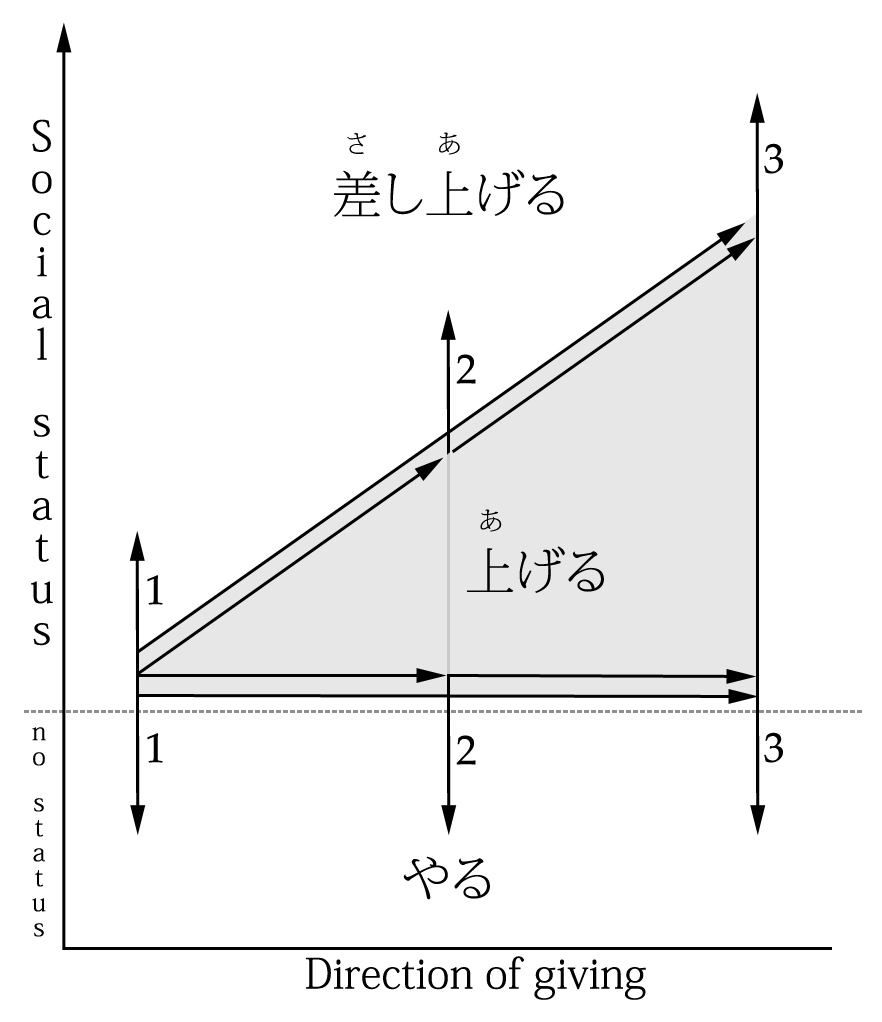
\includegraphics{../data/media/diagram-giving.jpg}}\nopagebreak[4]\par {\smaller \smaller A schematic representation of verbs involved in giving in Japanese}\end{center}


We see three “areas” in this image:

\begin{enumerate}
\item When giving to someone socially much higher‚ we must use \ruby{差}{さ}し\ruby{上}{あ}げる‚
\item when giving to someone who is either socially higher or equal‚ we must use \ruby{上}{あ}げる‚ and
\item when giving to someone (or something) without social status‚ we can use やる.
\end{enumerate}

\paragraph{Being given}


\vspace{0.5em}
\begin{center}
\fbox{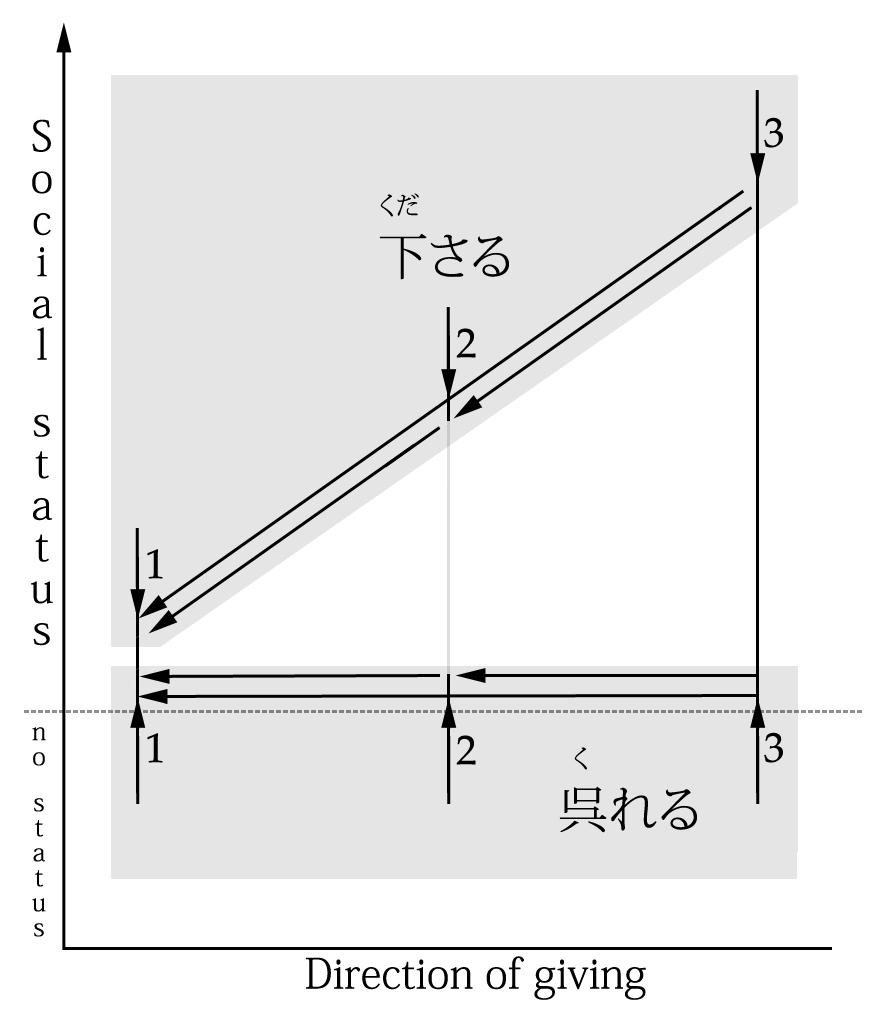
\includegraphics{../data/media/diagram-begiven.jpg}}\nopagebreak[4]\par {\smaller \smaller A schematic representation of verbs involved in ‘being given’ in Japanese}\end{center}


We see two “areas” in this image:

\begin{enumerate}
\item When being given something by someone who is socially higher‚ we describe their giving by using \ruby{下}{くだ}さる‚ and
\item when being given something by someone who is socially equal or lower‚ we describe their giving by using \ruby{呉}{く}れる.
\end{enumerate}

\paragraph{Receiving}


\vspace{0.5em}
\begin{center}
\fbox{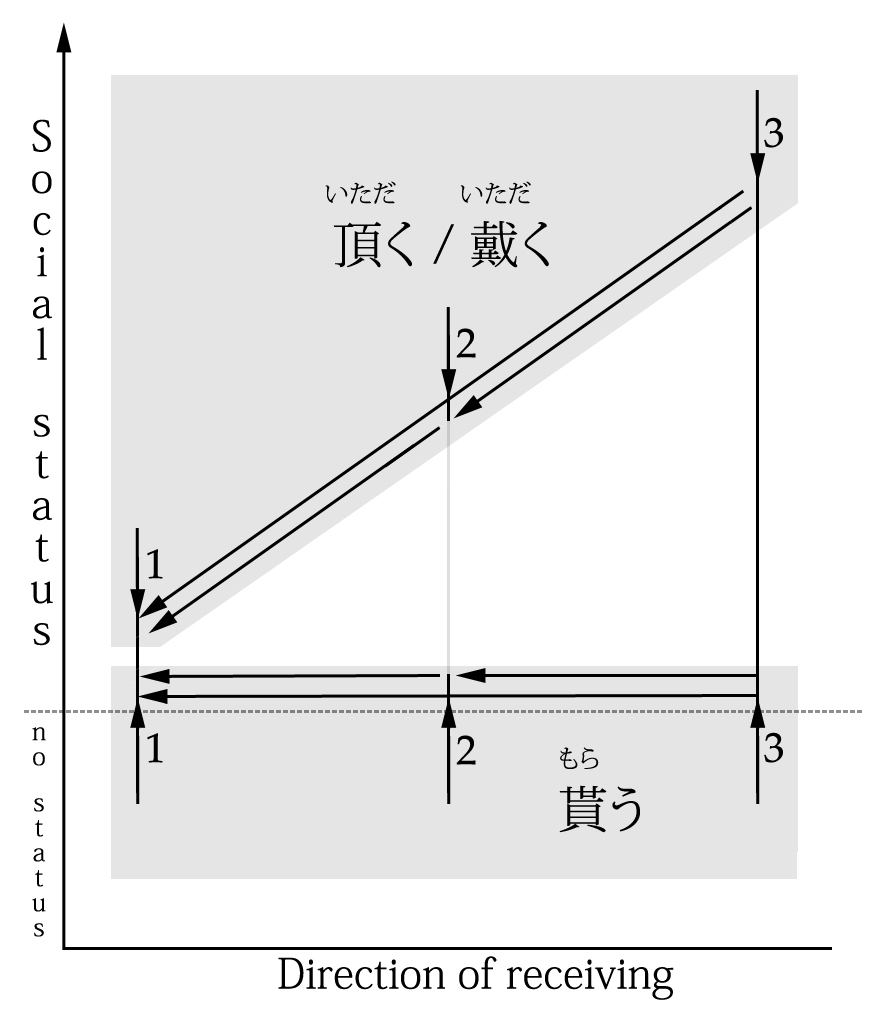
\includegraphics{../data/media/diagram-receiving.jpg}}\nopagebreak[4]\par {\smaller \smaller A schematic representation of verbs involved in receiving in Japanese}\end{center}


We see two “areas” in this image:

\begin{enumerate}
\item When receiving something from someone who is socially higher‚ we describe our receiving by using \ruby{頂}{いただ}く or \ruby{戴}{いただ}く (the choice of which to use being essentially arbitrary‚ as いただく is generally written in hiragana in this use)‚ and
\item when receiving something from someone who is socially equal or lower‚ we describe our receiving by using \ruby{貰}{もら}う.
\end{enumerate}

\subsection{\index[english]{Indirect speech}Indirect speech}

One of the important things in using Japanese is to be indirect whenever possible in formal situations. This entails asking indirect questions instead of direct questions‚ making indirect suggestions instead of telling people what they should do according to you‚ and stating assumptions rather than stating truths‚ even if they are truths. This section will explain how to turn direct speech into indirect speech‚ and for which constructions this is easily done.

\subsubsection{Expressing \index[english]{Hearsay}hearsay}

One way to state something indirectly is by making explicit the fact that you only heard or read something somewhere‚ rather than it being something that you believe or know. As mentioned in the section on comparison and likeness‚ this is done using the noun adjective \index[japanese]{そう}そう‚ in combination with a clause in 連体形‚ to form a hear-say construction. Compare the following two statements:

\vspace{0.4cm}
\begin{exampleblock}
あの\ruby{人気}{にんき}なグループが\ruby{解散}{かいさん}する。 \\* 
“That popular group will disband.” \\* 
\end{exampleblock}
\vspace{0.2cm}

\begin{exampleblock}
あの人気なグループが解散するそうだ。 \\* 
“I hear that popular group will disband.” \\* 
\end{exampleblock}
\vspace{0.2cm}

While the first sentence implies that the speaker is certain of the stated fact‚ the second sentence states the information more carefully‚ stating that it seems the case that something is a fact‚ based on having heard or read it somewhere. This indirect form of stating something can only be done for second hand information‚ and should never be used to soften a statement that isn’t actually hearsay.

\subsubsection{\index[english]{Negative questions}Negative questions}

Asking a negative question is‚ in many languages‚ a way to politely ask someone to do something. For instance‚ “won’t you join us for dinner?” is an English phrase that has the implied meaning “please join us for dinner”‚ rather than the literal “you will not be joining us for dinner‚ will you?”.

In Japanese the same applies:

\vspace{0.4cm}
\begin{exampleblock}
また\ruby{遊}{あそ}びに\ruby{来}{き}ませんか。 \\* 
“Won’t (you) come over (for a social visit) again some time?” \\* 
\end{exampleblock}
\vspace{0.2cm}

\begin{exampleblock}
(In this sentence 遊ぶ is not used to mean “play” but “to spend time leisurely”‚ hence the implied clause “for a social visit”) \\* 
\end{exampleblock}
\vspace{0.2cm}

A more polite way to ask \index[english]{Negative questions}negative questions is to use the て form with a negative form of 下さい:

\vspace{0.4cm}
\begin{exampleblock}
お\ruby{茶}{ちゃ}を\ruby{飲}{の}んで\ruby{下}{くだ}さいませんか。 \\* 
“Won’t (you) have some tea?” \\* 
\end{exampleblock}
\vspace{0.2cm}

These negative questions can also be formed with plain negative form‚ but they become more informal that way:

\vspace{0.4cm}
\begin{exampleblock}
ケーキを\ruby{食}{た}べない？ \\* 
“Won’t you have some (literally: eat) cake?” \\* 
\end{exampleblock}
\vspace{0.2cm}

Giving answers to negative questions can trip up beginning students quite easily‚ as the following example illustrates:

\vspace{0.4cm}
\begin{exampleblock}
A: \ruby{一緒}{いっしょ}に\ruby{行}{い}かない？ \\* 
B: はい。 \\* 
\end{exampleblock}
\vspace{0.2cm}

\begin{exampleblock}
A: “Won’t you go (with me)?” \\* 
B: “Yes (I won’t go with you).” \\* 
\end{exampleblock}
\vspace{0.2cm}

The problem lies with the fact that an affirmative answer to a negative question affirms the negative. Usually it is easier to answer with what you will be doing‚ rather than using yes or no:

\vspace{0.4cm}
\begin{exampleblock}
A: 一緒に行かない？ \\* 
B: 行きます。 \\* 
\end{exampleblock}
\vspace{0.2cm}

\begin{exampleblock}
A: “Won’t you go (with me)?” \\* 
B: “I will.” \\* 
\end{exampleblock}
\vspace{0.2cm}

An even better solution is to express your answer in the form of a motivation plus answer‚ when a negative question is asked‚ thus making it virtually impossible for your answer to be misinterpreted:

\vspace{0.4cm}
\begin{exampleblock}
A: 一緒に行かない？ \\* 
B: まあ‚ \ruby{暇}{ひま}だし、行きますよ。 \\* 
\end{exampleblock}
\vspace{0.2cm}

\begin{exampleblock}
A: “Won’t you go (with me)?” \\* 
B: “Well‚ (I’m) free (anyway)‚ (so) sure‚ I’ll go (with you).” \\* 
\end{exampleblock}
\subsubsection{\index[english]{Recommending}Recommending‚ using past tense + \index[japanese]{ほうがいい (方がいい)}\ruby{方}{ほう}がいい}


If we want to make a recommendation‚ there are various direct and indirect ways of doing so. One of the most common approaches uses a verb in plain past tense‚ paired with 方がいい‚ which creates a construction that essentially says “It might be better if you […]”.

\vspace{0.4cm}
\begin{exampleblock}
A: \ruby{遅}{お}くれてたから \ruby{彼女}{かのじょ}に\ruby{嫌}{きら}われてる。どうしよう。 \\* 
B: まあ、\ruby{謝}{あやま}った方がいいだろう？ \\* 
\end{exampleblock}
\vspace{0.2cm}

\begin{exampleblock}
A: “(My) girlfriend is angry with (me) because (I) was late. What should (I) do?” \\* 
B: “Well‚ wouldn’t it be sensible (literally: good) to apologise (to her)?” \\* 
\end{exampleblock}
\vspace{0.2cm}

This kind of recommendation is fairly direct‚ and thus some care must be taken in making sure that your relationship to whomever you make a recommendation to allows for this level of directness.

\subsubsection{\index[english]{Offering an opinion}Offering your opinion using \index[japanese]{…えば}-ば}

A less direct way of recommending something is by offering your own opinion. Using a hypothetical conditional paired with your own opinion on how good or bad this situation would be is a less direct way to suggest a course of action to someone. For instance:

\vspace{0.4cm}
\begin{exampleblock}
A: しまった。\ruby{間違}{まちが}いばかり\ruby{書}{か}いてた。 \\* 
B: \ruby{直}{なお}せばいいでしょう。 \\* 
\end{exampleblock}
\vspace{0.2cm}

\begin{exampleblock}
A: “Oh no‚ I’ve been writing mistakes all over the place.” \\* 
B: “Well‚ it won’t be that big of a deal if you just fix them?” \\* 
\end{exampleblock}
\vspace{0.2cm}

While this is of course still reasonably direct in the sense that you’re imposing your own opinion on someone‚ it is less direct than the previous past tense + 方がいい.

\subsubsection{\index[english]{Questioning suggestion}Asking about an option using \index[japanese]{…たらどう}-たらどう}

A truly indirect way of making a suggestion is by offering it as an option‚ without actually saying whether you think it’s the right course of action or not‚ effectively leaving the process of deciding whether it’s a good idea or not entirely up to the listener:

\vspace{0.4cm}
\begin{exampleblock}
A: どれほど\ruby{勉強}{べんきょう}してもこれが\ruby{分}{わ}かりませんよ。 \\* 
B: そうですか。じゃあ、\ruby{先生}{せんせい}に\ruby{聞}{き}いたらどうですか。 \\* 
\end{exampleblock}
\vspace{0.2cm}

\begin{exampleblock}
A: “No matter how much I study I don’t seem to understand this.” \\* 
B: “Hmm. Well‚ what about asking the teacher?” \\* 
\end{exampleblock}
\vspace{0.2cm}

This is the most polite way of making a suggestion‚ because it only stays at making the suggestion‚ without adding a personal recommendation to it‚ meaning you do not decide what the other person should do.

\subsubsection{Pseudo-future \index[english]{Suggesting}suggesting and \index[english]{Presumptive}presuming}

As you may remember from the section on the pseudo-future from chapter 3‚ the pseudo-future can be used for three things‚ namely the dubitative‚ \index[english]{Cohortative}cohortative and \index[english]{Presumptive}presumptive‚ and it turns out that these last two are ideal for use in indirect speech‚ as they guess at the world and leave the conclusions or decisions based on these guesses up to the listener‚ instead of imposing your own opinions on them:

\vspace{0.4cm}
\begin{exampleblock}
\ruby{今日}{きょう}はお\ruby{寿司}{すし}を\ruby{食}{た}べに\ruby{行}{い}こうか。 \\* 
“Shall (we) go (out) for sushi today?” \\* 
\end{exampleblock}
\vspace{0.2cm}

This question leaves the decision up to the listener‚ which is typically a polite thing to do‚ unless of course you’re dealing with someone who is bad at making decisions‚ in which case using indirect speech is arguably not a good idea in the first place.

\vspace{0.4cm}
\begin{exampleblock}
このコンピュータが\ruby{故障}{こしょう}してるのは、\ruby{古}{ふる}いからでしょう。 \\* 
“The reason this computer is broken is (probably) because it’s old (right?).” \\* 
\end{exampleblock}
\vspace{0.2cm}

In this sentence‚ the speaker assumes that the computer in question is old‚ and leaves the matter of whether this assumption is correct up to the listener to decide‚ thus not providing potential disinformation to the listener. Of course‚ this is an over-analysis‚ and these forms aren’t actually so much used to prevent disinformation as just used because indirect speech is polite‚ and that’s what you use. However‚ the analysis does hold up to scrutiny for a good reason: not presuming to know better means you’re never forcing anyone into anything‚ which makes you quite civilised.

\subsubsection{\index[english]{Double negative}Double negative statements}

In addition to these reasonably obvious suggestions‚ recommendations and opinions‚ we can also let our intentions shine through by using roundabout phrasing‚ thus softening our own convictions‚ opinions and intentions. The most common way this is done is by using double negative patterns‚ as described in the following sections.


\paragraph{\index[english]{Double negative!regular}Regular double negative}

The regular double negative construction is essentially the same as in English‚ relying on the presence of \glslink{volitional}{volitional} verbs (say‚ do‚ believe‚ promise‚ etc.):

\vspace{0.4cm}
\begin{exampleblock}
しないとは\ruby{言}{い}えません。 \\* 
“(I) cannot say (I) won’t do it.” \\* 
\end{exampleblock}
\vspace{0.2cm}

\begin{exampleblock}
\ruby{部長}{ぶちょう}に言わないとは\ruby{約束}{やくそく}しませんよ。 \\* 
“I won’t promise not to tell your boss.” \\* 
\end{exampleblock}
\vspace{0.2cm}

Note that in this use‚ the double negative is set up using と‚ in its role as ‘quoting’ particle.

However‚ there is a more frequently used double negative pattern in Japanese‚ used in a more subtle way to express an affirmative‚ which deserves special attention.


\paragraph{\index[english]{Double negative!complex}Complex double negative}

Frequently used‚ but certainly confusing the first time one sees or hears it‚ is the double negative hypothetical construction 未然形 + \index[japanese]{なければ}なければ + \index[japanese]{なければならない}ならない/\index[japanese]{なければいけない}いけない. While it uses two negatives to do its job‚ it’s actually used to imply an affirmative action instead. In a way‚ this makes sense: “I will not not-drink the coffee” has two negatives‚ but the first negates the second‚ so the sentence might as well read “I will drink the coffee”. We see the same happening in the Japanese complex double negative‚ but with an added nuance:

\vspace{0.4cm}
\begin{exampleblock}
\ruby{勉強}{べんきょう}しなければなりません。 \\* 
literally: “It should not become a fact that I am not studying” \\* 
meaning: “I really should go study.” \\* 
\end{exampleblock}
\vspace{0.2cm}

This construction requires some analysis: the construction is formed by inflecting a verb in plain negative form‚ 未然形 + ない‚ and turning this into a hypothetical: 未然形 + なけれ + ば. This negative hypothetical is then followed by either the negative form of なる‚ “become”‚ or the negative form of いける‚ which is a verb that expresses the figurative “will do” such as in “Yes‚ that will do nicely”. Because they express slightly different things‚ the choice of which to use depends on what a speaker wants to express.

Using 未然形 + なければ + ならない (or polite‚ using なりません) expresses that something “should” be done‚ i.e. that the negative verb action “should not come to be”. Using 未然形 + なければ + いけない (or polite‚ using いけません) expresses that something “has to” be done‚ i.e. that the negative verb action simply “will not do”. As such‚ ならない typically translates to a “need” to do something‚ whereas いけない typically translates to a “must”:

\vspace{0.4cm}
\begin{exampleblock}
ピアノの勉強をしなければなりません。 \\* 
“I (really) need to practise piano (now).” \\* 
\end{exampleblock}
\vspace{0.2cm}

In this sentence‚ there are no additional connotations: the speaker simply notes that they should practise piano. They might need to do so in order to improve‚ or because a recital is coming up‚ but this is left in the middle.

\vspace{0.4cm}
\begin{exampleblock}
ピアノの勉強をしなければいけません。 \\* 
“I must practise piano.” \\* 
\end{exampleblock}
\vspace{0.2cm}

In this sentence‚ there is the additional hidden information that not merely should the speaker practise‚ but that not practising will have undesirable consequences. Rather than just needing to practise‚ this practice has to be done to avoid whatever these undesirable consequences may be.

Colloquially‚ there are shorter versions of なければ‚ namely なけりゃ and なきゃ.  Because of the colloquial nature of the shorter forms‚ these are typically paired with the plain negatives ならない and いけない‚ as well as even more colloquial ならん and depending on who you talk to‚ いかん or あかん. The first is strictly speaking the short negative form of いく‚ rather than いける; the second is a word often associated with the dialects spoken in the Kansai region‚ although it is also used in other parts of Japan.

\section{More advanced grammar}

While there are a lot more topics available in the discussion of Japanese grammar‚ a selection had to be made for a book titled an “introduction” to Japanese. This book already covers more than what you would traditionally find in an introductory reader on the language‚ and sticking in even more topics would make it a far more complete work‚ but also tremendously more voluminous. As such‚ this is the end of this introduction to Japanese syntax‚ grammar and language. For further grammar‚ I can recommend picking up copies of the Dictionaries of Basic‚ Intermediary and Advanced Japanese Grammar by Seichi Makino and Michio Tsutsui‚ and referring to them whenever you run across interesting grammar use in Japanese material‚ or going on in search of more specialised dictionaries and reference works — there are plenty available!

\vspace{2em}

I hope you enjoyed this book‚ and I wish you all the best in your studies!


\clearpage

\appendix
\appendixpage
\addappheadtotoc

\renewcommand{\chaptername}{Appendix }

\chapter{Conjugation Schemes}
\nameheaders{Conjugation Schemes}

This appendix focuses entirely on the conjugation schemes that have been treated in this book‚ organised in two sections. The first lists all the base forms for the various verbals treated in this book‚ the second lists the actual conjugation tables for all these verbals. 

\section{Bases}

There are two sets of bases‚ one associated with \index[japanese]{ぶんご (文語)}\ruby{文語}{ぶんご}‚ classical (or literary) Japanese‚ and one associated with \index[japanese]{こうご (口語)}\ruby{口語}{こうご}‚ modern (or colloquial) Japanese. These are:

\vspace{0.5cm}
\smaller
\setlength\LTleft\parindent
\setlength\LTright\fill
\Needspace{6\baselineskip}
\begin{longtable}[h]{| l  l  l |}\hline
\rule{0pt}{2.4ex}base & 文語 & 口語\\ 
\hline 
\endfirsthead
\hline
\rule{0pt}{2.4ex}base & 文語 & 口語\\ 
\hline 
\endhead
\hline
\endfoot
\hline
\endlastfoot
\rule{0pt}{3.6ex}imperfect & \rtruby{未然形}{みぜんけい} & 未然形\\ 
\rule{0pt}{3.6ex}continuative & \rtruby{連用形}{れんようけい} & 連用形\\ 
\rule{0pt}{3.6ex}sentence ending & \rtruby{終止形}{しゅうしけい} & 連体形\\ 
\rule{0pt}{3.6ex}attributive & \rtruby{連体形}{れんたいけい} & 連体形\\ 
\rule{0pt}{3.6ex}perfect & \rtruby{已然形}{いぜんけい} & 已然形\\ 
\rule{0pt}{3.6ex}commanding & \rtruby{命令形}{めいれいけい} & 命令形\\ 
\end{longtable}
\larger
\vspace{0.5cm}


In addition to these bases‚ all verbal words have a stem‚ called the \index[japanese]{ごかん (語幹)}\ruby{語幹}{ごかん}‚ which is that part of the verbal that does not change during inflection.

On a functional note‚ the term “dictionary form” used in this chapter (and preceding chapters) refers the modern 連体形‚ which is the form used for listing verbal words in dictionaries. While synonymous‚ the term “dictionary form” will only be used to explain how to form bases. For everything else‚ the proper term 連体形 is used.



\Needspace{6\baselineskip}
\subsection{Regular verbs: \ruby{五段}{ごだん} verbs}

\smaller
\setlength\LTleft\fill
\setlength\LTright\fill
\begin{longtable}[h]{| l  l |}\hline
\rule{0pt}{2.4ex}base & how to form\\ 
\hline 
\endfirsthead
\hline
\rule{0pt}{2.4ex}base & how to form\\ 
\hline 
\endhead
\hline
\endfoot
\hline
\endlastfoot
\rule{0pt}{2.4ex}語幹 & remove final う—row syllable from dictionary form\\ 
\rule{0pt}{2.4ex}未然形 & final う—row syllable is replaced with the corresponding あ—row syllable\\ 
\rule{0pt}{2.4ex}連用形 & final う—row syllable is replaced with the corresponding い—row syllable\\ 
\rule{0pt}{2.4ex}連体形 & dictionary form ending on the う-row syllable\\ 
\rule{0pt}{2.4ex}已然形 & final う—row syllable is replaced with the corresponding え—row syllable\\ 
\rule{0pt}{2.4ex}命令形 & final う—row syllable is replaced with the corresponding え—row syllable\\ 
\end{longtable}
\larger

\Needspace{6\baselineskip}
\subsection{Regular verbs: \ruby{一段}{いちだん} verbs}

\smaller
\setlength\LTleft\parindent
\setlength\LTright\fill
\begin{longtable}[h]{| l  l |}\hline
\rule{0pt}{2.4ex}base & how to form\\ 
\hline 
\endfirsthead
\hline
\rule{0pt}{2.4ex}base & how to form\\ 
\hline 
\endhead
\hline
\endfoot
\hline
\endlastfoot
\rule{0pt}{2.4ex}語幹 & remove final る\\ 
\rule{0pt}{2.4ex}未然形 & remove final る\\ 
\rule{0pt}{2.4ex}連用形 & remove final る\\ 
\rule{0pt}{2.4ex}連体形 & dictionary form ending on る\\ 
\rule{0pt}{2.4ex}已然形 & replace final る with れ\\ 
\rule{0pt}{2.4ex}命令形 & remove final る\\ 
\end{longtable}
\larger

\Needspace{6\baselineskip}
\subsection{Irregular verbs: する (ずる/じる)}

\smaller
\begin{mytabular}{| l  l  l  l |}\hline 
\rule{0pt}{2.4ex}base & する & ずる & じる\\ 
\hline
\rule{0pt}{2.4ex}未然形 & さ‚ せ‚ し & ざ‚ ぜ‚ じ & じ\\ 
\rule{0pt}{2.4ex}連用形 & し & じ & じ\\ 
\rule{0pt}{2.4ex}連体形 & する & ずる & じる\\ 
\rule{0pt}{2.4ex}已然形 & すれ & ずれ & じれ\\ 
\rule{0pt}{2.4ex}命令形 & せ(よ)‚ し(ろ)‚ せい & ぜ(よ)‚ じ(ろ)‚ ぜい & じ(よ‚ ろ)\\ 
\hline 
\end{mytabular}
\larger
\vspace{0.5cm}


The 未然形 for these verbs follows special rules‚ because not all 未然形 forms are used for all inflections that require this base.

For the classical negation:

\begin{itemize}
\item する uses the せ—未然形
\item ずる uses the ぜ—未然形
\end{itemize}

For the (modern) passive and causative:

\begin{itemize}
\item する acts as either an 一段 or a 五段 verb for these forms; せ—未然形 + られる or さ—未然形 + れる to form the passive‚ さ—未然形 + せる to form the causative.
\item ずる acts as a normal 一段 verb‚ using just the じ—未然形‚ forming じられる for the passive and じさせる for the causative.
\item じる also acts as a normal 一段 verb‚ forming じられる for the passive and じさせる for the causative.
\end{itemize}
  
For the potential form‚ all three use \ruby{出来}{でき}る instead.


\Needspace{6\baselineskip}
\subsection{Irregular verbs: \ruby{来}{く}る}

\smaller
\begin{mytabular}{| l  l  l |}\hline 
\rule{0pt}{2.4ex}base & kanji form & pronunciation\\ 
\hline
\rule{0pt}{2.4ex}未然形 & 来 & こ\\ 
\rule{0pt}{2.4ex}連用形 & 来 & き\\ 
\rule{0pt}{2.4ex}連体形 & 来る & くる\\ 
\rule{0pt}{2.4ex}已然形 & 来れ & くれ\\ 
\rule{0pt}{2.4ex}命令形 & 来い & こい\\ 
\hline 
\end{mytabular}
\larger

\Needspace{6\baselineskip}
\subsection{Special verbs: ある}

\smaller
\begin{mytabular}{| l  l |}\hline 
\rule{0pt}{2.4ex}base & form\\ 
\hline
\rule{0pt}{2.4ex}未然形 & あら\\ 
\rule{0pt}{2.4ex}連用形 & あり\\ 
\rule{0pt}{2.4ex}連体形 & ある\\ 
\rule{0pt}{2.4ex}已然形 & あれ\\ 
\rule{0pt}{2.4ex}命令形 & あれ\\ 
\hline 
\end{mytabular}
\larger

\Needspace{6\baselineskip}
\subsection{Special verbs: だ}

\smaller
\begin{mytabular}{| l  l |}\hline 
\rule{0pt}{2.4ex}base & form\\ 
\hline
\rule{0pt}{2.4ex}未然形 & だろ\\ 
\rule{0pt}{2.4ex}連用形 & で (だつ)\\ 
\rule{0pt}{2.4ex}終止形 & だ\\ 
\rule{0pt}{2.4ex}連体形 & な\\ 
\rule{0pt}{2.4ex}已然形 & なら\\ 
\hline 
\end{mytabular}
\larger

\Needspace{6\baselineskip}
\subsection{Special verbs: です}

\smaller
\begin{mytabular}{| l  l |}\hline 
\rule{0pt}{2.4ex}base & form\\ 
\hline
\rule{0pt}{2.4ex}未然形 & でしょ\\ 
\rule{0pt}{2.4ex}連用形 & でし\\ 
\rule{0pt}{2.4ex}連体形 & です\\ 
\hline 
\end{mytabular}
\larger

\Needspace{6\baselineskip}
\subsection{Special verbs: ます}

\smaller
\begin{mytabular}{| l  l |}\hline 
\rule{0pt}{2.4ex}base &  form\\ 
\hline
\rule{0pt}{2.4ex}未然形 & ませ (ましょ)\\ 
\rule{0pt}{2.4ex}連用形 & まし\\ 
\rule{0pt}{2.4ex}連体形 & ます\\ 
\rule{0pt}{2.4ex}已然形 & ますれ\\ 
\rule{0pt}{2.4ex}命令形 & ませ (まし)\\ 
\hline 
\end{mytabular}
\larger

\Needspace{6\baselineskip}
\subsection{Verbal adjectives}

\smaller
\setlength\LTleft\parindent
\setlength\LTright\fill
\begin{longtable}[h]{| l  l |}\hline
\rule{0pt}{2.4ex}base & how to form\\ 
\hline 
\endfirsthead
\hline
\rule{0pt}{2.4ex}base & how to form\\ 
\hline 
\endhead
\hline
\endfoot
\hline
\endlastfoot
\rule{0pt}{2.4ex}語幹 & Remove the い from the dictionary form.\\ 
\rule{0pt}{2.4ex}未然形 & 語幹 + く\\ 
\rule{0pt}{2.4ex}連用形 & 語幹 + く\\ 
\rule{0pt}{2.4ex}連体形 & 語幹 + い\\ 
\rule{0pt}{2.4ex}已然形 & 語幹 + けれ\\ 
\rule{0pt}{2.4ex}(命令形 & 語幹 + かれ)\\ 
\end{longtable}
\larger

\Needspace{6\baselineskip}
\subsection{Special bases for \ruby{御座}{ござ}る}

\smaller
\begin{mytabular}{| l  l |}\hline 
\rule{0pt}{2.4ex}base & form\\ 
\hline
\rule{0pt}{2.4ex}未然形 & ござら\\ 
\rule{0pt}{2.4ex}連用形 & ござい\\ 
\rule{0pt}{2.4ex}連体形 & ござる\\ 
\rule{0pt}{2.4ex}已然形 & ござれ\\ 
\rule{0pt}{2.4ex}命令形 & ござい\\ 
\hline 
\end{mytabular}
\larger

\Needspace{6\baselineskip}
\subsection{Special bases for いらっしゃる}

\smaller
\begin{mytabular}{| l  l |}\hline 
\rule{0pt}{2.4ex}base & form\\ 
\hline
\rule{0pt}{2.4ex}未然形 & いらっしゃら\\ 
\rule{0pt}{2.4ex}連用形 & いらっしゃい\\ 
\rule{0pt}{2.4ex}連体形 & いらっしゃる\\ 
\rule{0pt}{2.4ex}已然形 & いらっしゃれ\\ 
\rule{0pt}{2.4ex}命令形 & いらっしゃい\\ 
\hline 
\end{mytabular}
\larger

\Needspace{6\baselineskip}
\subsection{Special bases for おっしゃる}

\smaller
\begin{mytabular}{| l  l |}\hline 
\rule{0pt}{2.4ex}base & form\\ 
\hline
\rule{0pt}{2.4ex}未然形 & おっしゃら\\ 
\rule{0pt}{2.4ex}連用形 & おっしゃい\\ 
\rule{0pt}{2.4ex}連体形 & おっしゃる\\ 
\rule{0pt}{2.4ex}已然形 & おっしゃれ\\ 
\rule{0pt}{2.4ex}命令形 & おっしゃい\\ 
\hline 
\end{mytabular}
\larger

\Needspace{6\baselineskip}
\subsection{Special bases for \ruby{下}{くだ}さる}

\smaller
\begin{mytabular}{| l  l |}\hline 
\rule{0pt}{2.4ex}base & form\\ 
\hline
\rule{0pt}{2.4ex}未然形 & 下さら\\ 
\rule{0pt}{2.4ex}連用形 & 下さい\\ 
\rule{0pt}{2.4ex}連体形 & 下さる\\ 
\rule{0pt}{2.4ex}已然形 & 下され\\ 
\rule{0pt}{2.4ex}命令形 & 下さい\\ 
\hline 
\end{mytabular}
\larger

\Needspace{6\baselineskip}
\subsection{Special bases for なさる}

\smaller
\begin{mytabular}{| l  l |}\hline 
\rule{0pt}{2.4ex}base & form\\ 
\hline
\rule{0pt}{2.4ex}未然形 & なさら\\ 
\rule{0pt}{2.4ex}連用形 & なさい\\ 
\rule{0pt}{2.4ex}連体形 & なさる\\ 
\rule{0pt}{2.4ex}已然形 & なされ\\ 
\rule{0pt}{2.4ex}命令形 & なさい\\ 
\hline 
\end{mytabular}
\larger
\section{Conjugation schemes}


\subsection{Regular verbs: \ruby{五段}{ごだん} verbs}

Contractions in the inflections are indicated with (c)

\vspace{0.5cm}
\smaller
\setlength\LTleft\fill
\setlength\LTright\fill
\Needspace{6\baselineskip}
\begin{longtable}[h]{| l  l  l  l |}\hline
\rule{0pt}{2.4ex}inflection & formality & affirmative & negative\\ 
\hline 
\endfirsthead
\hline
\rule{0pt}{2.4ex}inflection & formality & affirmative & negative\\ 
\hline 
\endhead
\hline
\endfoot
\hline
\endlastfoot
\rule{0pt}{2.4ex}present & informal & 連体形 & 未然形 + ん\\ 
\rule{0pt}{2.4ex} &  &  & 未然形 + ない\\ 
\rule{0pt}{2.4ex} & formal & 連用形 + ます & 連用形 + ません\\ 
\rule{0pt}{2.4ex}past & informal & 連用形 + た (c) & 未然形 + なかった\\ 
\rule{0pt}{2.4ex} & formal & 連用形 + ました & 連用形 + ませんでした\\ 
\rule{0pt}{2.4ex}て form & informal & 連用形 + て (c) & 未然形 + ないで\\ 
\rule{0pt}{2.4ex} &  &  & 未然形 + なくて\\ 
\rule{0pt}{2.4ex} & formal & 連用形 + まして & 連用形 + ませんで\\ 
\rule{0pt}{2.4ex}past conditional & informal & 連用形 + たら (c) & 未然形 + なかったら\\ 
\rule{0pt}{2.4ex} & formal & 連用形 + ましたら & 連用形 + ませんでしたら\\ 
\rule{0pt}{2.4ex}representative & informal & 連用形 + たり (c) & 未然形 + なかったり\\ 
\rule{0pt}{2.4ex} & formal & 連用形 + ましたり & 連用形 + ませんでしたり\\ 
\rule{0pt}{2.4ex}pseudo-future & informal & 未然形 + う (c) & 連体形 + まい\\ 
\rule{0pt}{2.4ex} & formal & 連用形 + ましょう & 連用形 + ますまい\\ 
\rule{0pt}{2.4ex}past pseudo-future & informal & 連用形 + たろう (c) & 未然形 + なかったろう\\ 
\rule{0pt}{2.4ex} & formal & 連用形 + ましたろう & 連用形 + ませんでしたろう\\ 
\rule{0pt}{2.4ex}presumptive & plain & 連体形 + だろう & 未然形 + ないだろう\\ 
\rule{0pt}{2.4ex} & polite & 連体形 + でしょう & 未然形 + ないでしょう\\ 
\rule{0pt}{2.4ex}past presumptive & plain & 連用形 + ただろう (c) & 未然形 + なかっただろう\\ 
\rule{0pt}{2.4ex} & polite & 連用形 + たでしょう (c) & 未然形 + なかったでしょう\\ 
\rule{0pt}{2.4ex}hypothetical & neutral & 已然形 + ば & 未然形 + なければ\\ 
\rule{0pt}{2.4ex} & emphatic & 連体形 + なら & 未然形 + ないなら\\ 
\rule{0pt}{2.4ex} & formal(1) & 連用形 + ませば & 連用形 + ませんなら\\ 
\rule{0pt}{2.4ex} & formal(2) & 連用形 + ますれば & \\ 
\rule{0pt}{2.4ex}commanding & informal & 命令形 & 連体形 + な\\ 
\rule{0pt}{2.4ex} &  & 連用形 + な & 未然形 + ないで\\ 
\rule{0pt}{2.4ex} &  & 連用形 + なさい & (連用形 + なさるな)\\ 
\rule{0pt}{2.4ex} &  & お + 連用形 + なさい & お + 連用形 +\\ 
\rule{0pt}{2.4ex} &  &  & 　　なさらないで\\ 
\rule{0pt}{2.4ex} & very formal & お + 連用形 + & お + 連用形 +\\ 
\rule{0pt}{2.4ex} &  & 　　なさいませ & 　　なさいますな\\ 
\rule{0pt}{3.6ex}requesting & neutral & 連用形 + & 未然形 + ないで\rtruby{下}{くだ}さい\\ 
\rule{0pt}{3.6ex} &  & 　　て\rtruby{下}{くだ}さい (c) & \\ 
\rule{0pt}{2.4ex} & formal & お + 連用形 + & お + 連用形 +\\ 
\rule{0pt}{3.6ex} &  & 　　なさって\rtruby{下}{くだ}さい & 　　なさらないで\rtruby{下}{くだ}さい\\ 
\rule{0pt}{2.4ex}passive‚ honorific‚ & informal & 未然形 + れる & 未然形 + れない\\ 
\rule{0pt}{2.4ex}potential & formal & 未然形 + れます & 未然形 + れません\\ 
\rule{0pt}{3.6ex}short potential & informal & 連用形 + \rtruby{得}{え}る (c) & 連用形 + えない (c)\\ 
\rule{0pt}{2.4ex} & formal & 連用形 + えます (c) & 連用形 + えません (c)\\ 
\rule{0pt}{2.4ex}causative & informal & 未然形 + せる & 未然形 + せない\\ 
\rule{0pt}{2.4ex} & formal & 未然形 + せます & 未然形 + せません\\ 
\rule{0pt}{2.4ex}causative passive & informal & 未然形 + せられる & 未然形 + せられない\\ 
\rule{0pt}{2.4ex} & formal & 未然形 + せられます & 未然形 + せられません\\ 
\rule{0pt}{2.4ex}humble & I & お + 連用形 + する & お + 連用形 + しない\\ 
\rule{0pt}{2.4ex} &  & お + 連用形 + します & お + 連用形 + しません\\ 
\rule{0pt}{3.6ex} & II & お + 連用形 + \rtruby{致}{いた}す & お + 連用形 + \rtruby{致}{いた}さない\\ 
\rule{0pt}{3.6ex} &  & お + 連用形 + \rtruby{致}{いた}します & お + 連用形 + \rtruby{致}{いた}しません\\ 
\rule{0pt}{2.4ex}honorific & I & お + 連用形 + に + なる & お + 連用形 + に +\\ 
\rule{0pt}{2.4ex} &  &  & 　　ならない\\ 
\rule{0pt}{2.4ex} &  & お + 連用形 + に + & お + 連用形 + に +\\ 
\rule{0pt}{2.4ex} &  & 　　なります & 　　なりません\\ 
\rule{0pt}{2.4ex} & II & お + 連用形 + なさる & お + 連用形 + なさらない\\ 
\rule{0pt}{2.4ex} &  & お + 連用形 + & お + 連用形 + なさいません\\ 
\rule{0pt}{2.4ex} &  & 　　なさいます & お + 連用形 + なさいません\\ 
\end{longtable}
\larger

\Needspace{6\baselineskip}
\subsection{Regular verbs: \ruby{一段}{いちだん} verbs}

\smaller
\setlength\LTleft\fill
\setlength\LTright\fill
\begin{longtable}[h]{| l  l  l  l |}\hline
\rule{0pt}{2.4ex}inflection & formality & affirmative & negative\\ 
\hline 
\endfirsthead
\hline
\rule{0pt}{2.4ex}inflection & formality & affirmative & negative\\ 
\hline 
\endhead
\hline
\endfoot
\hline
\endlastfoot
\rule{0pt}{2.4ex}present & informal &  & (未然形 + ぬ)\\ 
\rule{0pt}{2.4ex} &  & 連体形 & 未然形 + ない\\ 
\rule{0pt}{2.4ex} & formal & 連用形 + ます & 連用形 + ません\\ 
\rule{0pt}{2.4ex}past & informal & 連用形 + た & 未然形 + なかった\\ 
\rule{0pt}{2.4ex} & formal & 連用形 + ました & 連用形 + ませんでした\\ 
\rule{0pt}{2.4ex}て form & informal & 連用形 + て & 未然形 + ないで\\ 
\rule{0pt}{2.4ex} &  &  & 未然形 + なくて\\ 
\rule{0pt}{2.4ex} & formal & 連用形 + まして & 連用形 + ませんで\\ 
\rule{0pt}{2.4ex}past conditional & informal & 連用形 + たら & 未然形 + なかったら\\ 
\rule{0pt}{2.4ex} & formal & 連用形 + ましたら & 連用形 + ませんでしたら\\ 
\rule{0pt}{2.4ex}representative & informal & 連用形 + たり & 未然形 + なかったり\\ 
\rule{0pt}{2.4ex} & formal & 連用形 + ましたり & 連用形 + ませんでしたり\\ 
\rule{0pt}{2.4ex}pseudo-future & informal & 未然形 + よう & 未然形 + まい\\ 
\rule{0pt}{2.4ex} & formal & 連用形 + ましょう & 連用形 + ますまい\\ 
\rule{0pt}{2.4ex}past pseudo-future & informal & 連用形 + たろう & 未然形 + なかったろう\\ 
\rule{0pt}{2.4ex} & formal & 連用形 + ましたろう & 連用形 + ませんでしたろう\\ 
\rule{0pt}{2.4ex}presumptive & plain & 連体形 + だろう & 未然形 + ないだろう\\ 
\rule{0pt}{2.4ex} & polite & 連体形 + でしょう & 未然形 + ないでしょう\\ 
\rule{0pt}{2.4ex}past presumptive & plain & 連用形 + ただろう & 未然形 + なかっただろう\\ 
\rule{0pt}{2.4ex} & polite & 連用形 + たでしょう & 未然形 + なかったでしょう\\ 
\rule{0pt}{2.4ex}hypothetical & neutral & 已然形 + ば & 未然形 + なければ\\ 
\rule{0pt}{2.4ex} & emphatic & 連体形 + なら & 未然形 + ないなら\\ 
\rule{0pt}{2.4ex} & very formal & 連用形 + ませば & 連用形 + ませんなら\\ 
\rule{0pt}{2.4ex} &  & 連用形 + ますれば & \\ 
\rule{0pt}{2.4ex}commanding & informal & 命令形 + よ & \\ 
\rule{0pt}{2.4ex} &  & 命令形 + ろ & 連体形 + な\\ 
\rule{0pt}{2.4ex} &  & 連用形 + な & 未然形 + ないで\\ 
\rule{0pt}{2.4ex} &  & 連用形 + なさい & (連用形 + なさるな)\\ 
\rule{0pt}{2.4ex} & formal & お + 連用形 + なさい & お + 連用形 +\\ 
\rule{0pt}{2.4ex} &  &  & 　　なさらないで\\ 
\rule{0pt}{2.4ex} & very formal & お + 連用形 + & お + 連用形 +\\ 
\rule{0pt}{2.4ex} &  & 　　なさいませ & 　　なさいますな\\ 
\rule{0pt}{3.6ex}requesting & neutral & 連用形 + て\rtruby{下}{くだ}さい & 未然形 + ないで\rtruby{下}{くだ}さい\\ 
\rule{0pt}{2.4ex} & formal & お + 連用形 + & お + 連用形 +\\ 
\rule{0pt}{3.6ex} &  & 　　なさって\rtruby{下}{くだ}さい & 　　なさらないで\rtruby{下}{くだ}さい\\ 
\rule{0pt}{2.4ex}passive‚ honorific‚ & informal & 未然形 + られる & 未然形 + られない\\ 
\rule{0pt}{2.4ex}potential & formal & 未然形 + られます & 未然形 + られません\\ 
\rule{0pt}{2.4ex}causative & informal & 未然形 + させる & 未然形 + させない\\ 
\rule{0pt}{2.4ex} & formal & 未然形 + させます & 未然形 + させません\\ 
\rule{0pt}{2.4ex}causative passive & informal & 未然形 + させられる & 未然形 + させられない\\ 
\rule{0pt}{2.4ex} & formal & 未然形 + させられます & 未然形 + させられません\\ 
\rule{0pt}{2.4ex}humble & I & お + 連用形 + する & お + 連用形 + しない\\ 
\rule{0pt}{2.4ex} &  & お + 連用形 + します & お + 連用形 + しません\\ 
\rule{0pt}{3.6ex} & II & お + 連用形 + \rtruby{致}{いた}す & お + 連用形 + \rtruby{致}{いた}さない\\ 
\rule{0pt}{3.6ex} &  & お + 連用形 + \rtruby{致}{いた}します & お + 連用形 + \rtruby{致}{いた}しません\\ 
\rule{0pt}{2.4ex}honorific & I & お + 連用形 + に + なる & お + 連用形 + に +\\ 
\rule{0pt}{2.4ex} &  &  & 　　ならない\\ 
\rule{0pt}{2.4ex} &  & お + 連用形 + に + & お + 連用形 + に +\\ 
\rule{0pt}{2.4ex} &  & 　　なります & 　　なりません\\ 
\rule{0pt}{2.4ex} & II & お + 連用形 + なさる & お + 連用形 + なさらない\\ 
\rule{0pt}{2.4ex} &  & お + 連用形 + & お + 連用形 +\\ 
\rule{0pt}{2.4ex} &  & 　　なさいます & 　　なさいません\\ 
\end{longtable}
\larger

\Needspace{6\baselineskip}
\subsection{Irregular verbs: する (ずる/じる)}

\smaller
\setlength\LTleft\fill
\setlength\LTright\fill
\begin{longtable}[h]{| l  l  l  l |}\hline
\rule{0pt}{2.4ex}inflection & formality & affirmative & negative\\ 
\hline 
\endfirsthead
\hline
\rule{0pt}{2.4ex}inflection & formality & affirmative & negative\\ 
\hline 
\endhead
\hline
\endfoot
\hline
\endlastfoot
\rule{0pt}{2.4ex}present & informal &  & せ—未然形 + ん\\ 
\rule{0pt}{2.4ex} &  & 連体形 & 未然形 + ない\\ 
\rule{0pt}{2.4ex} & formal & 連用形 + ます & 連用形 + ません\\ 
\rule{0pt}{2.4ex}past & informal & 連用形 + た & 未然形 + なかった\\ 
\rule{0pt}{2.4ex} & formal & 連用形 + ました & 連用形 + ませんでした\\ 
\rule{0pt}{2.4ex}て form & informal & 連用形 + て & 未然形 + ないで\\ 
\rule{0pt}{2.4ex} &  &  & 未然形 + なくて\\ 
\rule{0pt}{2.4ex} & formal & 連用形 + まして & 連用形 + ませんで\\ 
\rule{0pt}{2.4ex}past conditional & informal & 連用形 + たら & 未然形 + なかったら\\ 
\rule{0pt}{2.4ex} & formal & 連用形 + ましたら & 連用形 + ませんでしたら\\ 
\rule{0pt}{2.4ex}representative & informal & 連用形 + たり & 未然形 + なかったり\\ 
\rule{0pt}{2.4ex} & formal & 連用形 + ましたり & 連用形 + ませんでしたり\\ 
\rule{0pt}{2.4ex}pseudo-future & informal & 未然形 + よう & 連体形 + まい\\ 
\rule{0pt}{2.4ex} & formal & 連用形 + ましょう & 連用形 + ますまい\\ 
\rule{0pt}{2.4ex}past pseudo-future & informal & 連用形 + たろう & 未然形 + なかったろう\\ 
\rule{0pt}{2.4ex} & formal & 連用形 + ましたろう & 連用形 + ませんでしたろう\\ 
\rule{0pt}{2.4ex}presumptive & plain & 連体形 + だろう & 未然形 + ないだろう\\ 
\rule{0pt}{2.4ex} & polite & 連体形 + でしょう & 未然形 + ないでしょう\\ 
\rule{0pt}{2.4ex}past presumptive & plain & 連用形 + ただろう & 未然形 + なかっただろう\\ 
\rule{0pt}{2.4ex} & polite & 連用形 + たでしょう & 未然形 + なかったでしょう\\ 
\rule{0pt}{2.4ex}hypothetical & neutral & 已然形 + ば & 未然形 + なければ\\ 
\rule{0pt}{2.4ex} & emphatic & 連体形 + なら & 未然形 + ないなら\\ 
\rule{0pt}{2.4ex} & formal (1) & 連用形 + ませば & 連用形 + ませんなら\\ 
\rule{0pt}{2.4ex} & formal (2) & 連用形 + ますれば & \\ 
\rule{0pt}{2.4ex}commanding & informal & せ-命令形 + よ & \\ 
\rule{0pt}{2.4ex} &  & し-命令形 + ろ & 連体形 + な\\ 
\rule{0pt}{2.4ex} &  & 連用形 + な & 未然形 + ないで\\ 
\rule{0pt}{2.4ex} & formal & なさい & なさらないで\\ 
\rule{0pt}{2.4ex} &  &  & (なさるな)\\ 
\rule{0pt}{2.4ex} & formal (2) & なさいませ & なさいますな\\ 
\rule{0pt}{3.6ex}requesting & neutral & 連用形 + て\rtruby{下}{くだ}さい & 未然形 + ないで下さい\\ 
\rule{0pt}{2.4ex} & formal & なさって下さい & なさらないで下さい\\ 
\rule{0pt}{2.4ex}passive‚ honorific & informal & see note & ～れない\\ 
\rule{0pt}{2.4ex} & formal & ～れます & ～れません\\ 
\rule{0pt}{2.4ex}causative & informal & see note & ～せない\\ 
\rule{0pt}{2.4ex} & formal & ～せます & ～せません\\ 
\rule{0pt}{2.4ex}causative passive & informal & see note & ～せられない\\ 
\rule{0pt}{2.4ex} & formal & ～せられます & ～せられません\\ 
\end{longtable}
\larger
\vspace{0.5cm}

\smaller
\begin{mytabular}{| l  l |}\hline 
\rule{0pt}{2.4ex}inflection & replacement verb\\ 
\hline
\rule{0pt}{3.6ex}humble & \rtruby{致}{いた}す\\ 
\rule{0pt}{2.4ex}honorific & なさる\\ 
\rule{0pt}{3.6ex}potential & \rtruby{出来}{でき}る\\ 
\hline 
\end{mytabular}
\larger

\Needspace{6\baselineskip}
\subsection{Irregular verbs: くる (来る)}

\smaller
\setlength\LTleft\fill
\setlength\LTright\fill
\begin{longtable}[h]{| l  l  l  l |}\hline
\rule{0pt}{2.4ex}inflection & formality & affirmative & negative\\ 
\hline 
\endfirsthead
\hline
\rule{0pt}{2.4ex}inflection & formality & affirmative & negative\\ 
\hline 
\endhead
\hline
\endfoot
\hline
\endlastfoot
\rule{0pt}{2.4ex}present & informal &  & 未然形 + ん (ぬ)\\ 
\rule{0pt}{2.4ex} &  & 連体形 & 未然形 + ない\\ 
\rule{0pt}{2.4ex} & formal & 連用形 + ます & 連用形 + ません\\ 
\rule{0pt}{2.4ex}past & informal & 連用形 + た & 未然形 + なかった\\ 
\rule{0pt}{2.4ex} & formal & 連用形 + ました & 連用形 + ませんでした\\ 
\rule{0pt}{2.4ex}て form & informal & 連用形 + て & 未然形 + ないで\\ 
\rule{0pt}{2.4ex} &  &  & 未然形 + なくて\\ 
\rule{0pt}{2.4ex} & formal & 連用形 + まして & 連用形 + ませんで\\ 
\rule{0pt}{2.4ex}past conditional & informal & 連用形 + たら & 未然形 + なかったら\\ 
\rule{0pt}{2.4ex} & formal & 連用形 + ましたら & 連用形 + ませんでしたら\\ 
\rule{0pt}{2.4ex}representative & informal & 連用形 + たり & 未然形 + なかったり\\ 
\rule{0pt}{2.4ex} & formal & 連用形 + ましたり & 連用形 + ませんでしたり\\ 
\rule{0pt}{2.4ex}pseudo-future & informal & 未然形 + よう & 未然形 + まい\\ 
\rule{0pt}{2.4ex} & formal & 連用形 + ましょう & 連用形 + ますまい\\ 
\rule{0pt}{2.4ex}past pseudo-future & informal & 連用形 + たろう & 未然形 + なかったろう\\ 
\rule{0pt}{2.4ex} & formal & 連用形 + ましたろう & 連用形 + ませんでしたろう\\ 
\rule{0pt}{2.4ex}presumptive & plain & 連体形 + だろう & 未然形 + ないだろう\\ 
\rule{0pt}{2.4ex} & polite & 連体形 + でしょう & 未然形 + ないでしょう\\ 
\rule{0pt}{2.4ex}past presumptive & plain & 連用形 + ただろう & 未然形 + なかっただろう\\ 
\rule{0pt}{2.4ex} & polite & 連用形 + たでしょう & 未然形 + なかったでしょう\\ 
\rule{0pt}{2.4ex}hypothetical & neutral & 已然形 + ば & 未然形 + なければ\\ 
\rule{0pt}{2.4ex} & emphatic & 連体形 + なら & 未然形 + ないなら\\ 
\rule{0pt}{2.4ex} & formal (1) & 連用形 + ませば & 連用形 + ませんなら\\ 
\rule{0pt}{2.4ex} & formal (2) & 連用形 + ますれば & \\ 
\rule{0pt}{2.4ex}commanding & informal & 命令形 & 連体形 + な\\ 
\rule{0pt}{2.4ex} &  & 連用形 + な & 未然形 + ないで\\ 
\rule{0pt}{2.4ex} &  & 連用形 + なさい & (連用形 + なさるな)\\ 
\rule{0pt}{3.6ex} & formal & お + \rtruby{出}{い}で + なさい & \\ 
\rule{0pt}{3.6ex} & very formal & お + \rtruby{出}{い}で + なさいませ & お + \rtruby{出}{い}で + なさいますな\\ 
\rule{0pt}{3.6ex}requesting &  & 連用形 + て\rtruby{下}{くだ}さい & 未然形 + ないで\rtruby{下}{くだ}さい\\ 
\rule{0pt}{2.4ex}passive‚ honorific & informal & 未然形 + られる & 未然形 + られない\\ 
\rule{0pt}{2.4ex}potential & formal & 未然形 + られます & 未然形 + られません\\ 
\rule{0pt}{2.4ex}causative & informal & 未然形 + させる & 未然形 + させない\\ 
\rule{0pt}{2.4ex} & formal & 未然形 + させます & 未然形 + させません\\ 
\rule{0pt}{2.4ex}causative passive & informal & 未然形 + させられる & 未然形 + させられない\\ 
\rule{0pt}{2.4ex} & formal & 未然形 + させられます & 未然形 + させられません\\ 
\end{longtable}
\larger
\vspace{0.5cm}

\smaller
\begin{mytabular}{| l  l |}\hline 
\rule{0pt}{2.4ex}inflection & replacement verb\\ 
\hline
\rule{0pt}{3.6ex}humble & \rtruby{参}{まい}る\\ 
\rule{0pt}{2.4ex}honorific & いらっしゃる\\ 
\hline 
\end{mytabular}
\larger
\subsection{Special verbs: ある}


Contractions in the inflections are indicated with (c)‚ standard Japanese indicated with (標準語).

\vspace{0.5cm}
\smaller
\setlength\LTleft\fill
\setlength\LTright\fill
\Needspace{6\baselineskip}
\begin{longtable}[h]{| l  l  l  l |}\hline
\rule{0pt}{2.4ex}inflection & formality & affirmative & negative\\ 
\hline 
\endfirsthead
\hline
\rule{0pt}{2.4ex}inflection & formality & affirmative & negative\\ 
\hline 
\endhead
\hline
\endfoot
\hline
\endlastfoot
\rule{0pt}{2.4ex}present & informal &  & ない (標準語)‚ 未然形 + ない\\ 
\rule{0pt}{2.4ex} & formal & 連用形 + ます & 連用形 + ません\\ 
\rule{0pt}{2.4ex}past & informal & 連用形 + た (c) & なかった\\ 
\rule{0pt}{2.4ex} & formal & 連用形 + ました & 連用形 + ませんでした\\ 
\rule{0pt}{2.4ex}て form & informal & 連用形 + て (c) & なくて\\ 
\rule{0pt}{2.4ex} & formal & 連用形 + まして & 連用形 + ませんで\\ 
\rule{0pt}{2.4ex}past conditional & informal & 連用形 + たら (c) & なかったら\\ 
\rule{0pt}{2.4ex} & formal & 連用形 + ましたら & 連用形 + ませんでしたら\\ 
\rule{0pt}{2.4ex}representative & informal & 連用形 + たり (c) & なかったり\\ 
\rule{0pt}{2.4ex} & formal & 連用形 + ましたり & 連用形 + ませんでしたり\\ 
\rule{0pt}{2.4ex}pseudo-future & informal & 未然形 + う (c) & 連体形 + まい\\ 
\rule{0pt}{2.4ex} & formal & 連用形 + ましょう & 連用形 + ますまい\\ 
\rule{0pt}{2.4ex}past pseudo-future & informal & 連用形 + たろう (c) & なかったろう\\ 
\rule{0pt}{2.4ex} & formal & 連用形 + ましたろう & 連用形 + ませんでしたろう\\ 
\rule{0pt}{2.4ex}presumptive & plain & 連体形 + だろう & なかろうないだろう\\ 
\rule{0pt}{2.4ex} & polite & 連体形 + でしょう & ないでしょう\\ 
\rule{0pt}{2.4ex}past presumptive & plain & 連用形 + ただろう (c) & なかっただろう\\ 
\rule{0pt}{2.4ex} & polite & 連用形 + たでしょう (c) & なかったでしょう\\ 
\rule{0pt}{2.4ex}hypothetical & neutral & 已然形 + ば & なければ\\ 
\rule{0pt}{2.4ex} & emphatic & 連体形 + なら & ないなら\\ 
\rule{0pt}{2.4ex} & formal (1) & 連用形 + ませば & 連用形 + ませんなら\\ 
\rule{0pt}{2.4ex} & formal (2) & 連用形 + ますれば & \\ 
\rule{0pt}{2.4ex}commanding & informal & 命令形  & \\ 
\rule{0pt}{2.4ex}passive‚ honorific & informal & 未然形 + れる & 未然形 + れない\\ 
\rule{0pt}{2.4ex}potential & formal & 未然形 + れます & 未然形 + れません\\ 
\rule{0pt}{3.6ex}short potential & informal & 連用形 + \rtruby{得}{え}る & 連用形 + えない\\ 
\rule{0pt}{2.4ex} & formal & 連用形 + えます & 連用形 + えません\\ 
\rule{0pt}{2.4ex}causative & informal & 未然形 + せる & 未然形 + せない\\ 
\rule{0pt}{2.4ex} & formal & 未然形 + せます & 未然形 + せません\\ 
\rule{0pt}{2.4ex}causative passive & informal & 未然形 + せられる & 未然形 + せられない\\ 
\rule{0pt}{2.4ex} & formal & 未然形 + せられます & 未然形 + せられません\\ 
\end{longtable}
\larger
\vspace{0.5cm}

\smaller
\begin{mytabular}{| l  l |}\hline 
\rule{0pt}{2.4ex}inflection & replacement verb\\ 
\hline
\rule{0pt}{2.4ex}polite & ござる\\ 
\hline 
\end{mytabular}
\larger

\Needspace{6\baselineskip}
\subsection{Special verbs: だ/です}

\smaller
\setlength\LTleft\parindent
\setlength\LTright\fill
\begin{longtable}[h]{| l  l  l  l |}\hline
\rule{0pt}{2.4ex}inflection & politeness & affirmative & negative\\ 
\hline 
\endfirsthead
\hline
\rule{0pt}{2.4ex}inflection & politeness & affirmative & negative\\ 
\hline 
\endhead
\hline
\endfoot
\hline
\endlastfoot
\rule{0pt}{2.4ex}present & plain & だ & じゃない\\ 
\rule{0pt}{2.4ex} &  &  & ではない\\ 
\rule{0pt}{2.4ex} & polite & です & じゃありません\\ 
\rule{0pt}{2.4ex} &  &  & ではありません\\ 
\rule{0pt}{2.4ex}past & plain & だった & じゃなかった\\ 
\rule{0pt}{2.4ex} &  &  & ではなかった\\ 
\rule{0pt}{2.4ex} & polite & でした & じゃありませんでした\\ 
\rule{0pt}{2.4ex} &  &  & ではありませんでした\\ 
\rule{0pt}{2.4ex}て form & plain & だって & じゃなくて\\ 
\rule{0pt}{2.4ex} &  &  & ではなくて\\ 
\rule{0pt}{2.4ex} & polite & でして & じゃありませんでして\\ 
\rule{0pt}{2.4ex} &  &  & ではありませんでして\\ 
\rule{0pt}{2.4ex}past conditional & plain & だったら & じゃなかったら\\ 
\rule{0pt}{2.4ex} &  &  & ではなかったら\\ 
\rule{0pt}{2.4ex} & polite & でしたら & じゃありませんなら\\ 
\rule{0pt}{2.4ex} &  &  & ではありませんなら\\ 
\rule{0pt}{2.4ex}representative & plain & だったり & じゃなかったり\\ 
\rule{0pt}{2.4ex} &  &  & ではなかったり\\ 
\rule{0pt}{2.4ex} & polite & でしたり & じゃありませんでしたり\\ 
\rule{0pt}{2.4ex} &  &  & ではありませんでしたり\\ 
\rule{0pt}{2.4ex}pseudo-future & plain & だろう & じゃなかろう\\ 
\rule{0pt}{2.4ex} &  &  & ではなかろう\\ 
\rule{0pt}{2.4ex} &  &  & じゃないだろう\\ 
\rule{0pt}{2.4ex} &  &  & ではないだろう\\ 
\rule{0pt}{2.4ex} & polite & でしょう & じゃありませんでしょう\\ 
\rule{0pt}{2.4ex} &  &  & ではありませんでしょう\\ 
\rule{0pt}{2.4ex}past pseudo-future & plain & だったろう & じゃなかったろう\\ 
\rule{0pt}{2.4ex} &  &  & ではなかったろう\\ 
\rule{0pt}{2.4ex} & polite & でしょう & じゃありませんでしょい\\ 
\rule{0pt}{2.4ex} &  &  & ではありませんでしょう\\ 
\rule{0pt}{2.4ex}hypothetical & I & なら & じゃなければ\\ 
\rule{0pt}{2.4ex} & II & ならば & ではなければ\\ 
\end{longtable}
\larger
\vspace{0.5cm}


Note that these verbs have special humble and honorific counterparts. For the humble copula‚ で+ござる is used‚ and for the honorific copula‚ で+いらっしゃる is used. The verbs for these forms have special bases‚ which are listed in their own section.


\Needspace{6\baselineskip}
\subsection{Special verbs: ます}

\smaller
\setlength\LTleft\parindent
\setlength\LTright\fill
\begin{longtable}[h]{| l  l  l |}\hline
\rule{0pt}{2.4ex}inflection & affirmative & negative\\ 
\hline 
\endfirsthead
\hline
\rule{0pt}{2.4ex}inflection & affirmative & negative\\ 
\hline 
\endhead
\hline
\endfoot
\hline
\endlastfoot
\rule{0pt}{2.4ex}present & 連体形 & 未然形 + ん\\ 
\rule{0pt}{2.4ex}past & 連用形 + た & 未然形 + んでした\\ 
\rule{0pt}{2.4ex}て form & 連用形 + て & 未然形 + んで\\ 
\rule{0pt}{2.4ex}past conditional & 連用形 + たら & 未然形 + んでしたら\\ 
\rule{0pt}{2.4ex}representative & 連用形 + たり & 未然形 + んでしたり\\ 
\rule{0pt}{2.4ex}pseudo-future & ましょう & 未然形 + んでしょう\\ 
\rule{0pt}{2.4ex}past pseudo-future & 連用形 + たろう & 未然形 + んでしたろう\\ 
\rule{0pt}{2.4ex}hypothetical & 未然形 + ば & 未然形 + んなら\\ 
\rule{0pt}{2.4ex} & 已然形 + ば & \\ 
\rule{0pt}{2.4ex}commanding & 命令形 & \\ 
\end{longtable}
\larger
\subsection{Verbal adjectives}


Contractions in the inflections are indicated with (c)

\vspace{0.5cm}
\smaller
\setlength\LTleft\fill
\setlength\LTright\fill
\Needspace{6\baselineskip}
\begin{longtable}[h]{| l  l  l  l |}\hline
\rule{0pt}{2.4ex}inflection & formality & affirmative & negative\\ 
\hline 
\endfirsthead
\hline
\rule{0pt}{2.4ex}inflection & formality & affirmative & negative\\ 
\hline 
\endhead
\hline
\endfoot
\hline
\endlastfoot
\rule{0pt}{2.4ex}present & informal & 連体形 & 未然形 + ない\\ 
\rule{0pt}{2.4ex} & formal & 連体形 + です & 連用形 + ありません\\ 
\rule{0pt}{2.4ex}past & informal & 連用形 + あった (c) & 未然形 + なかった\\ 
\rule{0pt}{2.4ex} & formal &  & 連用形 + ありませんでした\\ 
\rule{0pt}{2.4ex}て form & informal & 連用形 + て & 未然形 + ないで\\ 
\rule{0pt}{2.4ex} & formal &  & 未然形 + なくて\\ 
\rule{0pt}{2.4ex}past conditional & informal & 連用形 + あったら (c) & 未然形 + なかったら\\ 
\rule{0pt}{2.4ex} & formal &  & 連用形 + ありませんでしたら\\ 
\rule{0pt}{2.4ex}pseudo-future & informal & 連用形 + あろう (c) & 未然形 + なかろう\\ 
\rule{0pt}{2.4ex} &  &  & 未然形 + ないだろう\\ 
\rule{0pt}{2.4ex} & formal & 連体形 + でしょう & 未然形 + ないでしょう\\ 
\rule{0pt}{2.4ex} &  &  & 連用形 + ありませんでしょう\\ 
\rule{0pt}{2.4ex}past pseudo- & informal & 連用形 + あったろう(c) & 未然形 + なかったろう\\ 
\rule{0pt}{2.4ex}future &  &  & 未然形 + なかっただろう\\ 
\rule{0pt}{2.4ex} & formal & 連用形 + & 未然形 + なかったでしょう\\ 
\rule{0pt}{2.4ex} &  & 　　あったでしょう (c) & 連用形 + ありませんでしたろう\\ 
\rule{0pt}{2.4ex}hypothetical & neutral & 已然形 + ば & 未然形 + なければ\\ 
\rule{0pt}{2.4ex} & emphatic & 連体形 + なら & 未然形 + ないなら\\ 
\rule{0pt}{2.4ex}commanding & informal & 連用形 + あれ (c) & \\ 
\end{longtable}
\larger
\subsubsection{Classical adverb form}


The following table shows the rules for using verbal adjectives as adverbs to classical verbs such as ござる and \ruby{出}{い}でる.

\vspace{0.5cm}
\smaller
\begin{center}
\begin{mytabularcentered}{| l  l |}\hline 
\rule{0pt}{2.4ex}adjective written as … & becomes …\\ 
\hline
\rule{0pt}{2.4ex}語幹 ending in an あ-row syllable + い & 語幹 ending in an お-row syllable + う\\ 
\rule{0pt}{2.4ex}語幹 ending in an い-row syllable + い & 語幹 ending in an い-row ‘ゆ’ glide\\ 
\rule{0pt}{2.4ex}語幹 ending in an う-row syllable + い & the same 語幹 + う\\ 
\rule{0pt}{2.4ex}語幹 ending in an お-row syllable + い & the same 語幹 + う\\ 
\hline 
\end{mytabularcentered}
\end{center}
\larger
\vspace{0.5cm}


\chapter{Set phrases}
\nameheaders{Set Phrases}

Every language has its set phrases for things like thanking people‚ or excusing yourself‚ or phrases that are used idiomatically‚ meaning something other than what the words would literally imply‚ such as telling someone to “take a chair” or “make themselves at home”. This appendix lists several common Japanese phrases‚ and per phrase gives the grammatical decomposition that can be made given all the material that has been presented in this book‚ with the phrases being ordered according to Japanese custom (starting at あ through お‚ and ending at ん).

\section*{\ruby{上}{あ}がって\ruby{下}{くだ}さい — “Please come in”}

Coming from the verb 上がる (あがる)‚ this sentence literally says “please be raised”. Its non-literal meaning comes from the fact that the traditional Japanese house has a raised floor at the entrance‚ where one takes off one’s shoes and steps up into the house itself.

\section*{\ruby{有}{あり}\ruby{難}{がと}う\ruby{御}{ご}\ruby{座}{ざ}います — “Thank you”}

As mentioned in the adjective section‚ this is an example of classical adjective pronunciation‚ and is actually a long chain of conjugations:

\vspace{0.4cm}
\begin{exampleblock}
ある in 連用形 + \ruby{難}{がた}い in classical pronunciation + ござる in 連用形 + ます \\* 
↓ \\* 
あり + がとう + ござい + ます \\* 
↓ \\* 
ありがとうございます \\* 
\end{exampleblock}
\vspace{0.2cm}

This literally means “this is a difficult thing to accept”‚ stemming from the concept of becoming indebted to someone who helps you. As becoming (further) indebted to someone is always a hard thing to accept‚ this phrase is used instead of a separate word for thanking.

There are various ways to use this sentence‚ the most indebting being どうもありがとうございます‚ which adds the word どうも to the phrase‚ meaning “in all possible ways”‚ coming from the question pronoun どう (how‚ in what way) and the generalising pronoun suffix も.

Still formal indebting is ありがとうございます. Just ありがとう‚ however‚ is not polite. It comes down to saying “thanks”‚ and pays improper respect to people who do something for you and are of higher social status. Never just say ありがとう to your teacher for instance. Always use ありがとうございます.

This expression can either be used in present‚ or future‚ tense (ありがとうございます) or it can be used in past tense (ありがとうございました)‚ with the difference lying in when the thanking is being done: if it is after the fact‚ ありがとうございました will be used‚ and if it’s either prior to‚ or during whatever we’re being thankful for‚ ありがとうございます is used.

\section*{いいえ — Disagreement}

The Japanese version of “no”. Alternatives to いいえ are the more colloquial ううん‚ and the more emphatic いや.

\section*{いけない — “Oh no”‚ “this won’t do”}

This word is often used to express that something will not do‚ is about to be done wrong‚ or is at this very moment going wrong. It’s technically the short potential form of 行く‚ 行ける‚ and literally means “this cannot go”. Used in this way‚ it is typically written in hiragana only.

\section*{いただきます — Said when one is about to eat}

This statement literally means “I will accept [this]”‚ in the receiving meaning of accept‚ and is used when one is about to eat in the company of others. This is similar to‚ for instance‚ the Christian practice of giving thanks for the food about to be received‚ but without the religious aspect. When one is done eating‚ one uses ごちそうさまでした to indicate that one is done.

\section*{\ruby{行}{い}って\ruby{来}{き}ます — “I will go and come back”}

This is said when one leaves a place that one expects to come back to. The most obvious example is when one goes off for one’s job or school in the morning‚ when it is used to say goodbye to whoever is still in the house. The standard reply‚ if warranted‚ is いってらっしゃい.


\section*{いって(い)らっしゃい — Said when someone who will return‚ leaves.}

Literally this is the honorific version of the command \ruby{行}{い}って\ruby{来}{き}て‚ “go and come back”‚ where the speaker tells the listener to go on their business and come back afterwards. This phrase is said to people who are leaving a place where they are expected to return‚ such as their house‚ typically in response to 行ってきます. The first い in the いらっしゃい part of いってらっしゃい is typically omitted after a て form‚ similar to how the い in いる is typically omitted when used with the て form.

\section*{いらっしゃいませ — “Be welcome”}

This is literally the commanding form of the honorific verb いらっしゃる‚ and is used by tenants to welcome their customers into their place of business. It doesn’t technically mean “be welcome”‚ but that’s what it has come to be considered to mean.

\section*{お\ruby{帰}{かえ}りなさい — “Welcome back”}

This phrase is the typical response to ただいま‚ and welcomes someone back home‚ or back to a place that can be considered a base of departure‚ such as your office‚ when you went out for a power meeting with management and have returned unscathed.

This phrase is technically the honorific commanding form of 帰る‚ “to return [to some base]”:

\vspace{0.4cm}
\begin{exampleblock}
お + 帰る in 連用形 + なさる in 命令形 \\* 
↓ \\* 
お + 帰り + なさい \\* 
↓ \\* 
お帰りなさい \\* 
\end{exampleblock}
\section*{お\ruby{蔭様}{かげさま}で — “Thanks to you”}


This phrase is a typical reply to the question お元気ですか (“how do you do?”)‚ in which case it is usually preceded by an affirmative such as はい. It is also used frequently in situations where someone receives praise from someone who contributed to whatever the praise is for. Traditionally‚ a 陰 — meaning “shadow” or “shadow figure” — is used to mean someone who acts as the unseen driving force behind other people. Literally‚ saying お蔭様で means “due to your being like a shadow for me”‚ and can be interpreted as “because of [your] contributing actions‚ [I am where I am now‚ at this moment]”.

\section*{お\ruby{元気}{げんき}で — “Get better”‚ “stay well”}

This phrase can be considered the statement お元気でいて‚ “be well”‚ with the いて left off. It is used as a general parting phrase with people who you will not be seeing the very next day‚ such as when seeing an incidental friend off‚ as well as a parting phrase for people who can use well-wishing‚ such as friends who seem a bit down.

\section*{お\ruby{元気}{げんき}ですか — “How are you?”}

This is a terribly misused phrase by people who start to take an interest in Japanese‚ who mistaken it for “hello”.

お元気ですか literally asks “are you 元気”‚ which means that it asks whether someone is feeling good about things in general. This is something you do not ask someone every day‚ but only when you haven’t seen someone in a while‚ or when there is a reason to ask them‚ such as when someone has just recovered from an illness. In this last case‚ the question may also be of the form もう元気ですか‚ meaning “are you 元気 again (already)?”.

元気のない人‚ people who are not 元気‚ are typically depressed‚ gloomy‚ glum‚ down and out‚ and for all intents and purposes a mood killer for everyone around them. Asking these people whether they are 元気 is a bit like driving home the point that they aren’t happy with a big pointy stick‚ so instead the phrase 元気ないみたいですね is typically used‚ carefully remarking that they “do not seem very 元気”.

\section*{お\ruby{先}{さき}に — Said when leaving early}

Said when leaving earlier than you normally would (namely when everyone else leaves)‚ お先に literally says “before [you/everyone else]” and is short for お先に\ruby{失礼}{しつれい}します‚ itself short for お先に[…]、\ruby{失礼}{しつれい}します where the placehold is some action taken at a time that would be considered inappropriate. This can be met with three responses‚ namely either a set phrase such as お\ruby{疲}{つか}れ\ruby{様}{さま}でした‚ ご\ruby{苦労様}{くろさま}でした‚ or お先にどうぞ (in context typically translated as “okay” or “sure”‚ rather than a literal “go ahead”). Or‚ of course‚ it might be met with surprise at the act of leaving early for no clear reason.

\section*{お\ruby{邪魔}{じゃま}します — Entering someone’s house}

The noun 邪魔 means obstruction or interference‚ and this sentence is a particularly good example of Japanese formality: this phrase is used when one is invited into a house. Courtesy demands that you indicate that even though you have been invited‚ you will intrude upon their home life by accepting this invitation and entering their house.

Because this phrase literally means “I’ll be intruding”‚ it can also be used when one really is intruding‚ such as breaking up an intimate conversation because you need to talk to one of the conversationalists‚ or when barging in on people.

\section*{お\ruby{世話}{せわ}します — Treating someone}

世話 means caring‚ in the giveable caring kind of way. Paired with する‚ the combination \ruby{世話}{}(を)する means “to give care to someone” in the positive sense‚ and is generally understood as meaning you will be treating someone to something. This phrase is used‚ for instance‚ when picking up the tab for someone (this will naturally be paired with some refusal by the treatee‚ and insistence on the part of the treater‚ but this is part of the Japanese process of doing things for people).

\section*{お\ruby{世話}{せわ}になります — To be taken care of}

Pairing 世話 with the verb なる‚ “become”‚ the combination 世話になる means “to be taken care of by someone” in the positive sense. For instance‚ when someone is offering to do something for you like pay the bill after dinner‚ or take care of you when you’re sick and you wish to oblige them‚ you use the phrase お世話になります to indicate that you will be taken care of in some way by them.

\section*{お\ruby{大事}{だいじ}に(して) — “Take care”}

大事 is a “valuable thing”‚ in the figurative sense. When someone is told お大事にして\ruby{下}{くだ}さい‚ they are told to “please act in a way so that they are treating themselves as something valuable”. This full sentence is often shortened to just お大事に.

For instance‚ when saying goodbye to someone who you will not see in a while‚ you typically wish them お大事に so that you may meet them again in good health at some point in the future.

\section*{お\ruby{疲}{つか}れ\ruby{様}{さま}(です/でした) — “You’ve worked hard”}

お疲れ様 literally means “the appearance of tiredness”‚ and comes from the noun form of the verb 疲れる‚ “to tire”‚ prefixed with the honorific お and suffixed with the more classical likeness suffix \ruby{様}{さま}. This statement is used when someone has performed a tiring job‚ or when one goes home after a day of working.

\section*{お\ruby{腹}{なか}が\ruby{空}{す}きました — Being hungry}

One states that one is hungry by saying their stomach has become empty. Variations on this theme are the plain past tense instead of formal past tense お腹が空いた or with the subject marker omitted‚ お腹すいた. Colloquial versions are \ruby{腹}{はら}が\ruby{減}{へ}った (note the different pronunciation for 腹) or simply 腹減った.

\section*{お\ruby{願}{ねが}いします — “Please”}

Literally this phrase reads “(I) wish it”‚ but is commonly interpreted as meaning “please” in the context of prompting someone to do something for you. It comes from the verb 願う‚ to wish:

\vspace{0.4cm}
\begin{exampleblock}
お + 願う in 連用形 + する in 連用形 + ます \\* 
↓ \\* 
お + 願い + します \\* 
↓ \\* 
お願いします \\* 
\end{exampleblock}
\section*{お\ruby{早}{はよ}うございます — “Good morning”}


This phrase doesn’t actually contain the word “morning” in any way‚ which explains why it’s possible to use this phrase at later points in the day. Literally‚ this is the statement 早いです‚ only in humble classical form:

\vspace{0.4cm}
\begin{exampleblock}
早い in classical form + 連用形 of ござる + ます \\* 
↓ \\* 
おはよう + ござい + ます \\* 
↓ \\* 
お早うございます \\* 
\end{exampleblock}
\vspace{0.2cm}

This statement basically affirms that some meeting is reasonably early for when it occurs. For school goers‚ 8:30 am could be early; for bookmakers‚ 1 p.m. could be early. It all depends on when your daily routine day starts.

\section*{お\ruby{久}{ひさ}し\ruby{振}{ぶ}りです — “It’s been a long time”}

This phrase is actually grammatically quite interesting as it consists of a noun compound formed of the verbal adjective 久しい‚ “long (timed)” and the verb 振る‚ “to end/give up”‚ which as compound is turned into a noun and prefixed with the honorific particle お‚ covering all the major word groups (verb‚ adjective‚ noun and particle) in a single term:

\vspace{0.4cm}
\begin{exampleblock}
お + 久しい as 語幹 + 振る in 連用形 (suffering from a voiced pronunciation as compound) + です \\* 
↓ \\* 
お + 久し + ぶり + です \\* 
↓ \\* 
お久し振りです \\* 
\end{exampleblock}
\vspace{0.2cm}

This phrase is used when a silence between two people is broken after some time‚ be this in writing‚ by virtue of a phone call‚ or by actually seeing someone in person again.

\section*{おめでとうございます — Congratulations}

Literally this phrase is a combination of めでたい (meaning auspicious) in classical form paired with ござる:

\vspace{0.4cm}
\begin{exampleblock}
お + めでたい in classical form + ござる in 連用形 + ます \\* 
↓ \\* 
お + めでとう + ございます \\* 
↓ \\* 
おめでとうございます \\* 
\end{exampleblock}
\vspace{0.2cm}

This phrase can be used with a million and one words to congratulate on any number of things‚ usually following the て form of descriptions of what the congratulations are offered for:

\vspace{0.4cm}
\begin{exampleblock}
\ruby{結婚}{けっこん}しておめでとうございます。 \\* 
“Congratulations on getting married.” \\* 
\end{exampleblock}
\vspace{0.2cm}

\begin{exampleblock}
\ruby{誕生日}{たんじょうび}おめでとうございます。 \\* 
“Congratulations on your birthday.” \\* 
\end{exampleblock}
\vspace{0.2cm}

\begin{exampleblock}
\ruby{卒業}{そつぎょう}しておめでとうございます。 \\* 
“Congratulations on graduating.” \\* 
\end{exampleblock}
\vspace{0.2cm}

et cetera‚ et cetera.

\section*{お\ruby{休}{やす}みなさい — “Good night”}

This phrase is said when one goes to bed‚ and is repeated by those who wish you a good night. It is technically the honorific commanding form of 休む‚ to rest‚ and is used to wish everyone else a good night too.

\vspace{0.4cm}
\begin{exampleblock}
お + 休む in 連用形 + なさる in 命令形 \\* 
↓ \\* 
お + 休み + なさい \\* 
↓ \\* 
お休みなさい \\* 
\end{exampleblock}
\section*{\ruby{気}{き}を\ruby{付}{つ}けて(\ruby{下}{くだ}さい) — “Take care”‚ “Be careful”}


Literally‚ this phrase instructs someone to apply 気‚ in this case best translated as “vigilance”‚ to whatever it is they are‚ or will be‚ doing. It is used when you wish someone to be careful‚ such as when they are about to do something potentially dangerous — whether it’s rewiring a wall socket‚ or heading out in a storm at midnight without a torch — or when they’re going to be in an environment that may be hazardous in some way — be it starting a school term at a new school‚ or going off to do your job as a fireman.

\section*{ご\ruby{苦労様}{くろうさま}(です/でした) — “Job well done”}

Literally‚ this phrase doesn’t say “well done” at all‚ but actually translates to “it would appear that you have exerted considerable effort”‚ 苦労 (くろう)‚ with the fact that this was actually “good” effort only being implied by the fact that you’re not being told you’ve done a bad job instead. This phrase can be used whenever someone has finished doing a tough job‚ or has had a rough day‚ but is typically reserved as a response to those of equal or lower standing.

This phrase is also used as a reply to お\ruby{先}{さき}に‚ when used by someone for whom it’s okay to leave work before others do (even if only by a few minutes). Colloquially the 様 in ご苦労様 can be replaced with さん‚ to create the more relaxed sounding ご苦労さん.

\section*{ご\ruby{馳走様}{ちそうさま}(でした) — Said when one is done eating}

This expression has no usable translation because it’s a customary saying. Literally this phrase means “it was a feast”‚ stemming from the noun \ruby{馳走}{ちそう} which means banquet and all the things a banquet entails such as good food and decent entertainment‚ and the likeness suffix \ruby{様}{さま}.

This phrase is the counterpart to the customary saying いただきます‚ said prior to consuming anything in the company of others.

\section*{ご\ruby{免}{めん}\ruby{下}{くだ}さい — “Please excuse me”}

This phrase is used in two common settings. The first is when hanging up on a phone conversation when you are the one hanging up‚ and the second is when you’re entering a place which you know is someone else’s‚ but you don’t see anyone around. Literally‚ 免 means dismissal‚ and this phrase asks for the listener to please dismiss your behaviour as it is intrinsically rude.

\section*{ご\ruby{免}{めん}なさい — “Please forgive me”}

This construction is more oriented towards asking for forgiveness rather than just being excused. When you have done something wrong‚ and you know you did‚ apologise with ごめんなさい.

This phrase is also used to turn down important offers‚ where the act of turning down the offer may lead to problems for the other party (such as when someone is depending on you‚ or when someone confesses their love for you).

When being specific about what you are asking forgiveness for‚ ごめんなさい follows the description in て form:

\vspace{0.4cm}
\begin{exampleblock}
ケーキを\ruby{食}{た}べて、ごめんなさい。 \\* 
“I’m sorry for eating (your) cake.” \\* 
\end{exampleblock}
\section*{\ruby{今日}{こんにち}は — “Good day”}


This is the particle は (pronounced わ)‚ added to the noun 今日 meaning “day” (pronounced こんにち instead of きょう). It’s technically an unfinished phrase just raising the topic of “today” and then saying absolutely nothing in regards to it‚ but this has become the standard way to say “good day” in Japanese.

\section*{\ruby{今晩}{こんばん}は — “Good evening”}

Like こんにちは‚ this is just は added to 今晩‚ “this evening”.

\section*{さようなら — “Farewell”}

Realise the full meaning of this word before you use it: さようなら is short for \ruby{左様}{さよう}ならばお\ruby{暇}{いとま}を\ruby{申}{もう}します‚ which is old Japanese for “Things being as they are‚ I shall speak my farewells”. The modern version‚ too‚ really does mean “farewell” and not just a plain “good bye”. There is a very explicit connotation that it will be a considerable time until the speaker will see again the person they’re seeing off‚ if ever.

\section*{\ruby{仕方}{しかた}がない — “There is nothing (…) can do about it”}

This phrase is quite often (and to the horror of many a translator) translated literally as “there is no helping it”. Now‚ the number of times you will hear that phrase used in English is probably a very small number indeed‚ and as such this phrase is much better translated with “there’s nothing [I/he/she/we] can do about it”.

仕方 is a conceptual noun for a “something that can be done”‚ and is an example of kanji being applied to a reading instead of the other way around: this is actually the “way of doing” construction for する‚ し方‚ where し has been given the kanji 仕‚ meaning doing/service. Variations on this theme involve omitting が‚ 仕方ない‚ or replacing し方 with the more humble \ruby{致}{いた}し方‚ and ない with the more polite ありません‚ leading to statements such as 致し方がありません.

\section*{\ruby{失礼}{しつれい}しました — “I have committed a rudeness”}

This is used as an excuse after the facts‚ when admitting that one has committed a rudeness.

\section*{\ruby{失礼}{しつれい}します — “Excuse me”}

失礼 literally means “a rudeness”‚ and 失礼する means to commit a rudeness. When one has to excuse oneself from somewhere‚ for instance‚ when one is talking to a superior and is called away for some reason‚ or one has to go before the conversation is truly over‚ this expression is used (in combination with the appropriate level of bowing) to indicate that one is aware that one’s actions will be somewhat rude.

\section*{じゃあ、また — “See you again (later)”}

This phrase is an unfinished phrase that literally means “well then‚ again [some other time]”‚ and is used as an informal goodbye when you expect to see each other again soon. The じゃあ comes from では‚ which in turn is short for それでは meaning “with this” or “by this” as context. また (又) means “again”‚ and so the whole sentence can be unwrapped to それでは、また[…]‚ where the final part of the sentence can be things like \ruby{明日}{あした}‚ “tomorrow”‚ \ruby{後}{あと}で‚ “later”‚ and so forth. Because of all this dropping of terms‚ there are several statements that can be used which all mean the same thing‚ but varying in level of formality:

\vspace{0.5cm}
\smaller
\setlength\LTleft\parindent
\setlength\LTright\fill
\Needspace{6\baselineskip}
\begin{longtable}[h]{| l  l |}\hline 
\endfirsthead
\hline 
\endhead
\hline
\endfoot
\hline
\endlastfoot
\rule{0pt}{2.4ex}それでは、また後で。 & formal polite\\ 
\rule{0pt}{2.4ex}では、また後で。 & formal polite\\ 
\rule{0pt}{2.4ex}では、また。 & casual polite\\ 
\rule{0pt}{2.4ex}じゃあ、また。 & informal\\ 
\rule{0pt}{2.4ex}じゃ、また。 & informal\\ 
\rule{0pt}{2.4ex}またね。 & very informal\\ 
\end{longtable}
\larger
\section*{\ruby{済}{す}みません — “Thank you”‚ “Excuse me”}


A prime example that Japanese conceptualises certain things differently‚ すみません can actually mean “thank you” and “excuse me” at the same time when used. While meaning a simple “excuse me” if used when (for instance) bumping into someone in the street‚ it is also used when someone does something for you that will indebt you to them‚ such as catching your hat and handing it back if the wind catches it‚ or fixing some typos in an email you had written. Using すみません in these instances means both “thank you for doing this for me” as well as “I’m sorry to have caused you to do this for me” at the same time.

This is technically the polite negative of \ruby{済}{す}む‚ “to end”‚ indicating that the debt between the two parties involved remains unsettled. Variations on the theme include the more colloquial すいません and very informal すまない and すまん.

When being specific about what you are thanking apologetically for‚ すみません follows the description in て form.

\vspace{0.4cm}
\begin{exampleblock}
\ruby{手伝}{てつだ}ってすみません。 \\* 
“Thank you for helping out‚ and sorry for somehow having made you do so.” \\* 
\end{exampleblock}
\section*{そうですか — “Is that so?”‚ “Really”‚ “I see”‚ “Aha”}


This is a typical phrase that doesn’t mean what it seems to mean‚ even if half the time it does. Much like how half the time when a Japanese person says はい‚ they won’t mean “yes” but are only indicating they’re listening‚ そうですか is used to acknowledge that the speaker is still being listened to just as much as it’s used to genuinely ask “is that so?”.

Only the context of the conversation is an indicator whether it’s just a polite way to show that someone is still being listened to‚ or whether the listener is genuinely wondering about something said.

\section*{そうですね — Showing agreement}

This phrase is often used when someone wants to emphatically agree in a conversation. It may also be used to indicate that the speaker has heard what has just been said and will respond to it‚ similar to はい. Misinterpreting it can lead to quite a bit of confusion:

\vspace{0.4cm}
\begin{exampleblock}
A: もう\ruby{終}{お}わってますか。 \\* 
B: そうですね。まだ終わってません。 \\* 
\end{exampleblock}
\vspace{0.2cm}

\begin{exampleblock}
A: “Have you finished yet?” \\* 
B: “Ah‚ yes… not yet.” \\* 
\end{exampleblock}
\vspace{0.2cm}

Here‚ B is first merely acknowledging that they heard the question‚ possibly even indicating that they think it’s a good question‚ and the real answer comes after そうですね.

\section*{ただいま  — “I’m back”‚ “Right away”}

There are three meanings to this phrase‚ although typically you will only be familiar with the first: when returning from something that one had to leave for (at which point an いってきます would have been used)‚ this phrase is used to signal the return. It is usually met with お\ruby{帰}{かえ}りなさい‚ an idiomatic expression translating to “welcome back”. 

The second meaning is quite different. When given an order to perform some task‚ using ただいま as response idiomatically translates to “right away”. This use is typical in settings where someone is commanded to do something‚ such as in a master/servant relationship.

Lastly‚ ただいま can also be used as a formal version of just \ruby{今}{いま}‚ meaning “now”. In this meaning‚ you may also find it used a lot in the expression ただいまより[…]‚ in which より is used in its classical (literary) meaning‚ being the same as the modern particle から‚ with the expression translating to “starting now”‚ “as of now” or “from this moment on”.

\section*{\ruby{頼}{たの}む — “Please”}

This is just the verb 頼む‚ “to leave in someone’s care”‚ but is frequently used as an expression both when offloading something to someone else (which can be considered quite rude)‚ to mean “please do this for me”‚ or when someone offers to do something for you and is giving off all the signals that they’re being serious instead of being polite‚ as an implicit “thank you”.

\section*{どう\ruby{致}{いた}しまして - “Don’t mention it”‚ “you’re welcome”}

This phrase is used in response to an expression of gratitude. Similar to how in English one might be polite by responding to “Thank you very much” with “you’re welcome” or “it was my pleasure”‚ this phrase acts as both an acknowledgement of the gratitude‚ as well as an indicator that the gratitude should not be experienced to the degree that the person doing the thanking is expressing (similar to how in English one might go “no‚ no‚ it was nothing”).

Grammatically speaking this construction is the humble version of どうして‚ but idiomatically these two expressions mean wildly different things‚ with どういたしまして being used to acknowledge or waive gratitude‚ and どうして being used to enquire the “why” of something.

\section*{どうした — “What happened?”}

Being a combination of the pronoun どう‚ “how” or “in what way”‚ and the past tense of する‚ this literally asks “by what way did […] happen?”. However‚ it is interpreted to mean “what happened?”‚ instead. どうした is a short question to enquire what happened when someone seems upset‚ taken aback‚ or give off the impression that something happened that is unusual. A more formal way to ask this‚ though also more effeminate‚ is どうかしましたか.

\section*{どうして(ですか) — “Why?”‚ “How come?”}

This is the combination of どう‚ “how”‚ and the verb する in て form. Using just どうして is technically an incomplete sentence‚ and implies that it should be finished with whatever verb best describes the situation that is being questioned. For instance‚ if someone refuses to help‚ the full sentence could be どうして\ruby{手伝}{てつだ}わないんですか‚ “why won’t you help?”‚ but just saying どうして is enough to act as question.

\section*{どうぞ — Urging someone‚ “If it pleases you‚ …”}

One of the power words in Japanese social language‚ どうぞ is used whenever you wish to politely urge someone to do something. For instance‚ if one has just served tea to guests and wishes to urge the guests to start drinking‚ a どうぞ combined with a sweeping hand gesture at the cups will convey the message that they should start drinking.

This word can frequently be heard in combination with urging requests‚ forming a more polite version of the request. For instance‚ the earlier entry \ruby{上}{あ}がって(ください) could be made more polite by turning it into どうぞ上がって(ください).

\section*{どうぞお\ruby{先}{さき}に — “After you”}

A common form of politeness in Japan (although arguably in any culture) is to repress your own feelings and desires so that others might benefit. Of the many ways in which this can be expressed‚ probably the most common way is letting other people do something before you get a chance to do them‚ such as opening a door for someone else to pass through first‚ or letting someone else queue up before you queue up.

The phrase combines どうぞ with 先に (“before”) in honorary form‚ translating to -- if we’re translating the intention of the expression rather than the literal words -- “If it pleases [you]‚ [allow me to let you do whatever I wanted to do] before [I do so‚ too]”.

\section*{どうぞよろしく — “Pleased to meet you”}

“Pleased to meet you” is actually the “best cultural approximation” translation. The Japanese statement doesn’t actually mean “pleased to meet you” at all‚ but relies on knowing what よろしく means. Being a noun derived from よろしい‚ “agreeable/acceptable”‚ this statement literally says that the speaker hopes that everything that is the result of this meeting is of a good nature. It’s only used once‚ when you first meet someone in a setting where you will work together in some capacity‚ and is more accurately described as saying “please treat me well in our future dealings”.

The more formal version is どうぞよりしくお\ruby{願}{ねが}いします‚ which adds the verb for “wishing” to the statement‚ thus expressing a sincere wish to be treated favourably in the future.

The short form‚ just よろしく‚ can be used in a broader setting to indicate you will leave something to someone under the assumption that all will be well‚ and is similar to \ruby{頼}{たの}む in this use.

\section*{なぜ(ですか) — “Why?”}

This is the most direct version of “why”‚ and is a pure interrogative; it’s short‚ and literally means “what reason”. Being the most direct‚ it’s also quite rude‚ and there is no polite way to use this word‚ so it’s best to try and avoid using it at all. Because it is technically a noun‚ it can be used in a softer form using です‚ but even then this is still considered more direct than asking the other two versions of “why” with です: \ruby{何}{なん}でですか or どうしてですか.

\section*{\ruby{何}{なん}で(ですか) — “Why?”}

This particular version of “why” is considered more direct than どうして‚ but less direct than なぜ. It is indirect in that it literally asks “by which means [do you reason this way]?” or “by which means [did this situation arise]?”‚ but is more direct because it’s shorter than どうして and thus sounds more curt.


\section*{\ruby{喉}{のど}が\ruby{渇}{かわ}いています — Being thirsty}

When one is thirsty in Japan‚ one doesn’t say “I am thirsty” but instead uses the less direct statement “my throat is dry”‚ similar to how one could say “I am a bit parched” in English rather than saying “I’m a bit thirsty”.

\section*{はい — Acknowledgement}

While generally understood to mean “yes”‚ はい actually signifies acknowledgement in general — it can be used as an acknowledging response to questions‚ in which case it means the same as “yes”‚ but it can also be used to indicate that some speaker is still being listened to. Like そうですね‚ this may lead to situations where はい can be interpreted as either:

\vspace{0.4cm}
\begin{exampleblock}
A: じゃあ、\ruby{分}{わ}かってますね。 \\* 
B: はい。分かりません。 \\* 
\end{exampleblock}
\vspace{0.2cm}

\begin{exampleblock}
A: “So‚ (you) know (what this means)‚ (don’t you).” \\* 
B: [acknowledges the question] “No.” \\* 
\end{exampleblock}
\vspace{0.2cm}

Alternatives to はい are the more colloquial うん and the more explicitly acknowledging そう.

\section*{\ruby{始}{はじ}めまして — A formal greeting used when meeting someone for the first time}

Like どうして‚ this is technically an unfinished sentence‚ being the polite て form of 始める‚ “to start (something)”‚ and comes from the original expression 初めてお\ruby{目}{め}にかかります literally translating to an acknowledgement that “this is the first time I have come before you”. Consequently‚ 初めまして is used as a set phrase greeting when meeting someone for the first time. In a setting where there will be a lasting cooperation between you and whoever you say this to‚ the conversation will typically steer towards どうぞよろしく or よろしくお\ruby{願}{ねが}いします‚ depending on the whether you will be potentially relying on the other person a lot.

\section*{\ruby{腹}{はら}が\ruby{立}{た}つ — Getting upset}

This phrase literally means “to raise [my] stomach”‚ and is used to indicate something causes genuine upset or upset anger. Like being hungry or thirsty‚ being upset‚ too‚ is typically indicated by describing the physical feeling.

\section*{\ruby{申}{もう}し\ruby{訳}{わけ}ありません — Extreme apology}

Literally this phrase reads “[this is] not [a situation in which] saying [something] [is appropriate]”. Effectively it means “I have no excuse [for what I have done]” and makes it clear that the speaker is genuinely at fault for something. Grammatically decomposing the phrase‚ we see:

\vspace{0.4cm}
\begin{exampleblock}
申す in 連用形 + meaning/reason nominaliser 訳 + formal polite negation of ある \\* 
申し + 訳 + ありません \\* 
\end{exampleblock}
\vspace{0.2cm}

Variations on this theme involve more‚ or less‚ formal versions of the verbs “to say” and “be”‚ such as 申し訳ない‚ \ruby{言}{い}い訳ない‚ 申し訳ございません‚ etc.

\section*{もしもし — Said when picking up the phone}

The story goes that this word was used because demons cannot pronounce it‚ and it would allow people to tell whether a real person had picked up the phone on the other end. Regardless of whether it’s true (it’s not‚ もしもし comes from \ruby{申}{もう}し\ruby{申}{もう}し‚ from the humble verb \ruby{申}{もう}す)‚ it makes for a nice story to tell people when they get curious about the phrase that the Japanese use when they pick up the phone‚ or when it appears the signal has dropped during a conversation.

This phrase is also used to call someone’s attention when they seem to be lost staring into the distance‚ similar to how one might yell “helloooo?” to someone who seems to have started day dreaming‚ in English.
% everything in this file comes at the end of our TeX document, and is considered backmatter

\backmatter

\glsidxheaders

% show the glossaries
\cleardoublepage
\phantomsection
\addcontentsline{toc}{chapter}{Glossary}
\markboth{Glossary}{}

\printglossaries

% show the indexes
\cleardoublepage
\phantomsection
\addcontentsline{toc}{chapter}{Index}

\markboth{Index - English}{}
\printindex[english]

\markboth{Index - Japanese}{}
\printindex[japanese]

% and finally end the document
\end{document}